%!TEX root = modelguide.tex <- not sure what this does

\def\maindoc{}% let subchapters know the entire manual is being typeset
\def\doctitle{ArtiSynth Modeling Guide}

% starting definitions for both the main document and stand-alone chapters
\documentclass{book}

\def\mech{artisynth.core.mechmodels}
\def\mgeo{maspack.geometry}

% Add search paths for input files
\makeatletter
\def\input@path{{../}{../../}{../texinputs/}}
\makeatother

\usepackage{amsmath}
\usepackage{framed}
%%
%% Default settings for artisynth
%%
\NeedsTeXFormat{LaTeX2e}
%%\ProvidesPackage{artisynthDoc}[2012/04/05]

\usepackage[T1]{fontenc}
\usepackage[latin1]{inputenc}
\usepackage{listings}
\usepackage{makeidx}
\usepackage{latexml}
\usepackage{graphicx}
\usepackage{framed}
\usepackage{booktabs}
\usepackage{color}

\newcommand{\pubdate}{\today}
\newcommand{\setpubdate}[1]{\renewcommand{\pubdate}{#1}}
\newcommand{\code}[1]{{\tt #1}}

\iflatexml
\usepackage{hyperref}
\setlength\parindent{0pt} 
\else
%% then we are making a PDF, so include things that LaTeXML can't handle: 
%% docbook style, \RaggedRight
\usepackage{ifxetex}
\usepackage{xstring}
\usepackage{pslatex} % fixes fonts; in particular sets a better-fitting \tt font

\usepackage[most]{tcolorbox}
\definecolor{shadecolor}{rgb}{0.95,0.95,0.95}
\tcbset{
    frame code={}
    center title,
    left=0pt,
    right=0pt,
    top=0pt,
    bottom=0pt,
    colback=shadecolor,
    colframe=white,
    width=\dimexpr\textwidth\relax,
    enlarge left by=0mm,
    boxsep=0pt,
    arc=0pt,outer arc=0pt,
}%

\usepackage[A4]{artisynth_papersize}
%\usepackage[letter]{artisynth_papersize}
\usepackage[hyperlink]{asciidoc-dblatex} 

%\usepackage{verbatim}
\usepackage{ragged2e}
\setlength{\RaggedRightRightskip}{0pt plus 4em}
\RaggedRight
\renewcommand{\DBKpubdate}{\pubdate}
\renewcommand{\DBKreleaseinfo}{}
\fi

% set hypertext links to be dark blue:
\definecolor{darkblue}{rgb}{0,0,0.8}
\definecolor{sidebar}{rgb}{0.5,0.5,0.7}
\hypersetup{colorlinks=true,urlcolor=darkblue,linkcolor=darkblue,breaklinks=true}

%%%%%%%%%%%%%%%%%%%%%%%%%%%%%%%%%%%%%%%%%%%%%%%%%%%%%%%%%%%%%%%%%%%%%%%%%%%%%
%
% Define macros for handling javadoc class and method references
%
%%%%%%%%%%%%%%%%%%%%%%%%%%%%%%%%%%%%%%%%%%%%%%%%%%%%%%%%%%%%%%%%%%%%%%%%%%%%%
\makeatletter

% macro to enable line break if inside a PDF file
\def\pdfbreak{\iflatexml\else\\\fi}

% code inspired by http://stackoverflow.com/questions/2457780/latex-apply-an-operation-to-every-character-in-a-string
\def\removeargs #1{\doremoveargs#1$\wholeString\unskip}
\def\doremoveargs#1#2\wholeString{\if#1$%
\else\if#1({()}\else{#1}\taketherest#2\fi\fi}
\def\taketherest#1\fi
{\fi \doremoveargs#1\wholeString}

% Note: still doesn't work properly when called on macro output ...
% i.e., \dottoslash{\concatnames{model}{base}{foo}} fails 
\def\dottoslash #1{\dodottoslash#1$\wholeString\unskip}
\def\dodottoslash#1#2\wholeString{\if#1$%
\else\if#1.{/}\else{#1}\fi\dottaketherest#2\fi}
\def\dottaketherest#1\fi{\fi \dodottoslash#1\wholeString}

\def\hashtodot #1{\dohashtodot#1$\wholeString\unskip}
\def\dohashtodot#1#2\wholeString{\if#1$X%
\else\if#1\#{.}\else{#1}\fi\hashtaketherest#2\fi}
\def\hashtaketherest#1\fi{\fi \dohashtodot#1\wholeString}

%\dollartodot{#1} does the same thing as \StrSubstitute[0]{#1}{\$}{.}
% from the packahe xstring. We define \dollartodot instead because
% LaTeXML does not implement xstring.
%
% Note that for the substituion to work, we need \ifx instead of \if,
% since otherwise escaped characters won't work properly:
% if #1 = \$, then \if#1* seems to compare '\' and '$' (and output '*'),
% rather than comparing '$' to '*'
\def\dollartodot #1{\dodollartodot#1*\wholeString\unskip}
\def\dodollartodot#1#2\wholeString{\ifx#1*%
\else \ifx#1\${.}\else{#1}\fi\dollartaketherest#2\fi}
\def\dollartaketherest#1\fi{\fi \dodollartodot#1\wholeString}

% concatenates up to three class/method names together, adding '.' characters
% between them. The first and/or second argument may be empty, in which case
% the '.' is omitted. To check to see if these arguments are empty, we
% use a contruction '\if#1@@', which will return true iff #1 is empty
% (on the assumption that #1 will not contain a '@' character).
\def\concatnames
#1#2#3{\if#1@@\if#2@@#3\else #2.#3\fi\else\if#2@@#1.#3\else#1.#2.#3\fi\fi}

\newcommand{\javabase}{}
\newcommand{\setjavabase}[1]{\renewcommand{\javabase}{#1}}

\def\artisynthDocBase{@ARTISYNTHDOCBASE}

\iflatexml
\def\ifempty#1{\def\temp{#1}\ifx\temp\empty}%
\newcommand{\artisynthManual}[3][]{%
   \ifempty{#1}
      \href{@ARTISYNTHDOCBASE/#2/#2.html}{#3}%
    \else
      \href{@ARTISYNTHDOCBASE/#1/#2.html}{#3}%
    \fi
}
\else
\newcommand{\artisynthManual}[3][]{%
\href{https://www.artisynth.org/@ARTISYNTHDOCBASE/#2.pdf}{#3}}
\fi

%\href{@ARTISYNTHDOCBASE/#2/#2.html}{#3}}



\newcommand{\javaclassx}[2][]{%
% Includes code to prevent an extra '.' at the front if #1 is empty. It
% works like this: if '#1' is empty, then '#1.' expands to '.', and so 
% '\if#1..' will return true, in which case we just output '#2'.
\href{@JDOCBEGIN/\concatnames{\javabase}{#1}{#2}@JDOCEND}{#2}}
\newcommand{\javaclass}[2][]{%
\href{@JDOCBEGIN/\concatnames{}{#1}{#2}@JDOCEND}{\dollartodot{#2}}}
\newcommand{\javaclassAlt}[2]{%
\href{@JDOCBEGIN/\concatnames{}{}{#1}@JDOCEND}{#2}}

\newcommand{\javamethodArgsx}[2][]{%
\href{@JDOCBEGIN/\concatnames{\javabase}{#1}{#2}@JDOCEND}{#2}}
\newcommand{\javamethodArgs}[2][]{%
\href{@JDOCBEGIN/\concatnames{}{#1}{#2}@JDOCEND}{#2}}
\newcommand{\javamethodAlt}[2]{%
\href{@JDOCBEGIN/\concatnames{}{}{#1}@JDOCEND}{#2}}
\newcommand{\javamethodAltx}[2]{%
\href{@JDOCBEGIN/\concatnames{\javabase}{}{#1}@JDOCEND}{#2}}

\newcommand{\javamethodNoArgsx}[2][]{%
\href{@JDOCBEGIN/\concatnames{\javabase}{#1}{#2}@JDOCEND}{\removeargs{#2}}}
\newcommand{\javamethodNoArgs}[2][]{%
\href{@JDOCBEGIN/\concatnames{}{#1}{#2}@JDOCEND}{\removeargs{#2}}}

\newcommand{\javamethod}{\@ifstar\javamethodNoArgs\javamethodArgs}
\newcommand{\javamethodx}{\@ifstar\javamethodNoArgsx\javamethodArgsx}

%%%%%%%%%%%%%%%%%%%%%%%%%%%%%%%%%%%%%%%%%%%%%%%%%%%%%%%%%%%%%%%%%%%%%%%%%%%%%
%
% Define macros for sidebars
%
%%%%%%%%%%%%%%%%%%%%%%%%%%%%%%%%%%%%%%%%%%%%%%%%%%%%%%%%%%%%%%%%%%%%%%%%%%%%%

\iflatexml
\newenvironment{sideblock}{\begin{quote}}{\end{quote}}
\else
\usepackage[strict]{changepage}
\definecolor{sidebarshade}{rgb}{1.0,0.97,0.8}
\newenvironment{sideblock}{%
    \def\FrameCommand{%
    \hspace{1pt}%
    {\color{sidebar}\vrule width 2pt}%
    %{\vrule width 2pt}%
    {\color{sidebarshade}\vrule width 4pt}%
    \colorbox{sidebarshade}%
  }%
  \MakeFramed{\advance\hsize-\width\FrameRestore}%
  \noindent\hspace{-4.55pt}% disable indenting first paragraph
  \begin{adjustwidth}{}{7pt}%
  %\vspace{2pt}\vspace{2pt}%
}
{%
  \vspace{2pt}\end{adjustwidth}\endMakeFramed%
}
\fi

\iflatexml
\newenvironment{shadedregion}{%
  \definecolor{shadecolor}{rgb}{0.96,0.96,0.98}%
  \begin{shaded*}%
% Put text inside a quote to create a surrounding blockquote that
% will properly accept the color and padding attributes
  \begin{quote}%
}
{%
  \end{quote}%
  \end{shaded*}%
}
\else
\newenvironment{shadedregion}{%
  \definecolor{shadecolor}{rgb}{0.96,0.96,0.98}%
  \begin{shaded*}%
}
{%
  \end{shaded*}%
}
\fi

% Wanted to create a 'listing' environment because lstlisting is
% tedious to type and because under latexml it may need
% some massaging to get it to work properly. But hard to do
% because of the verbatim nature of listing
%\iflatexml
%\newenvironment{listing}{\begin{lstlisting}}{\end{lstlisting}}%
%\else
%\newenvironment{listing}{\begin{lstlisting}}{\end{lstlisting}}%
%\fi

\iflatexml\else
% fancyhdr was complaining that it wanted a 36pt header height ...
\setlength{\headheight}{36pt}
\fi

% macro for backslash character
\newcommand\BKS{\textbackslash}

% macro for double hyphen (to prevent conversion of -- into -)
\newcommand\DHY{-{}-}

% Convenience stuff
\newcommand{\ifLaTeXMLelse}[2]{%
  \iflatexml %
  #1 %
  \else %
  #2 %
  \fi %
}

\newcommand{\ifLaTeXML}[1]{ %
  \iflatexml %
  #1 %
  \fi %
}

% new methodtable environment for documenting methods

% base width of the method table
\newlength{\methodtablewidth}
\iflatexml
\setlength{\methodtablewidth}{1.4\textwidth}
\else
\setlength{\methodtablewidth}{0.94\textwidth}
\fi
% horizontal space added at end of call to \methodentry
\newlength{\methodskip}
\setlength{\methodskip}{0pt}
% lengths set inside methodtable environment:
\newlength{\methodsiglength} % length of the method signature
\newlength{\methodcomlength} % length of the method comment
\setlength{\methodsiglength}{0.5\methodtablewidth}
\setlength{\methodcomlength}{0.5\methodtablewidth}

% command to add a method to a method table:
% arg #1: package and signature for finding URL
% arg #2: anchor text
% arg #3: comment describing the method
\newcommand{\methodentry}[3]{%
\javamethodAlt{#1}{\parbox[t]{\methodsiglength}{#2}}&
{\parbox[t]{\methodcomlength}{#3}}\\%
\noalign{\vspace{\methodskip}}}

% methodtable environment takes two arguments, both scale factors for
% methodtablewidth:
% arg #1: width of the method signature column
% arg #2: width of the method comment column
\newenvironment{methodtable}[3][0pt]{%
\begingroup
\setlength{\topskip}{0pt}
\setlength{\methodskip}{#1}
\setlength{\methodsiglength}{#2\methodtablewidth}%
\setlength{\methodcomlength}{#3\methodtablewidth}%
\iflatexml
\begin{snugshade}
\else
\begin{tcolorbox}
\fi
\renewcommand{\arraystretch}{1}
\begin{tabular}{ll}}{%
\end{tabular}
\renewcommand{\arraystretch}{1}
\iflatexml
\end{snugshade}
\else
\end{tcolorbox}
\fi
\endgroup}

% commands for added top, mid and bottom lines in the table.
% uses booktabs for PDF, regular hline for HTML
\newcommand{\topline}{\iflatexml\hline\else\toprule\fi}
\newcommand{\midline}{\iflatexml\hline\else\midrule\fi}
\newcommand{\botline}{\iflatexml\hline\else\bottomrule\fi}
\newcommand{\blankline}{%
\multicolumn{2}{l}{\iflatexml{@SPACE}\else\phantom{M}\fi}\\}%
% add vertical space within a two colum method environment
\newcommand{\methodspace}[1]{%
\iflatexml
\multicolumn{2}{l}{@VERTSPACE[#1]}\\
\else
\noalign{\vspace{#1}}%
\fi}%
% break a line and add an indentation of 1em
\newcommand{\brh}{\\\phantom{M}}

\makeatother

\def\matl{\left(\begin{matrix}}
\def\matr{\end{matrix}\right)}

\def\Bthe{\boldsymbol\theta}
\def\Btau{\boldsymbol\tau}
\def\Bom{\boldsymbol\omega}
\def\Bdel{\boldsymbol\delta}
\def\Blam{\boldsymbol\lambda}
\def\Bphi{\boldsymbol\phi}
\def\Bxi{\boldsymbol\xi}
\def\Bgam{\boldsymbol\gamma}
\def\Bsig{\boldsymbol\sigma}
\def\Bnu{\boldsymbol\nu}
\def\Bmu{\boldsymbol\mu}

\def\A{{\bf A}}
\def\B{{\bf B}}
\def\C{{\bf C}}
\def\D{{\bf D}}
\def\F{{\bf F}}
\def\G{{\bf G}}
\def\H{{\bf H}}
\def\I{{\bf I}}
\def\J{{\bf J}}
\def\K{{\bf K}}
\def\Jc{{\bf J}_c}
\def\L{{\bf L}}
\def\M{{\bf M}}
\def\N{{\bf N}}
\def\O{{\bf O}}
\def\P{{\bf P}}
\def\Q{{\bf Q}}
\def\R{{\bf R}}
\def\T{{\bf T}}
\def\U{{\bf U}}
\def\W{{\bf W}}
\def\X{{\bf X}}
\def\Minv{{\bf M}^{-1}}

\def\a{{\bf a}}
\def\b{{\bf b}}
\def\c{{\bf c}}
\def\d{{\bf d}}
\def\e{{\bf e}}
\def\f{{\bf f}}
\def\g{{\bf g}}
\def\k{{\bf k}}
\def\l{{\bf l}}
\def\m{{\bf m}}
\def\n{{\bf n}}
\def\p{{\bf p}}
\def\q{{\bf q}}
\def\r{{\bf r}}
\def\u{{\bf u}}
\def\v{{\bf v}}
\def\w{{\bf w}}
\def\x{{\bf x}}
\def\y{{\bf y}}
\def\z{{\bf z}}

\def\ma{{\bf m}_\alpha}
\def\mb{{\bf m}_\beta}
\def\va{{\bf v}_\alpha}
\def\vb{{\bf v}_\beta}
\def\vp{{\bf v}_\rho}
\def\vk{{\bf v}_k}
\def\ua{{\bf u}_\alpha}
\def\ub{{\bf u}_\beta}
\def\uk{{\bf u}_k}
\def\uj{{\bf u}_j}
\def\mar{{\bf m}_{\alpha r}}
\def\mbr{{\bf m}_{\beta r}}

\def\Maa{{\bf M}_{\alpha\alpha}}
\def\Mab{{\bf M}_{\alpha\beta}}
\def\Mba{{\bf M}_{\beta\alpha}}
\def\Mbb{{\bf M}_{\beta\beta}}
\def\hatMaa{\hat{\bf M}_{\alpha\alpha}}
\def\hatMab{\hat{\bf M}_{\alpha\beta}}
\def\hatMba{\hat{\bf M}_{\beta\alpha}}
\def\hatMbb{\hat{\bf M}_{\beta\beta}}
\def\Mbp{{\bf M}_{\beta\rho}}
\def\Map{{\bf M}_{\alpha\rho}}
\def\Mpa{{\bf M}_{\rho\alpha}}
\def\Mpb{{\bf M}_{\rho\beta}}
\def\Mpp{{\bf M}_{\rho\rho}}
\def\Mbk{{\bf M}_{\beta k}}
\def\Mak{{\bf M}_{\alpha k}}
\def\Mka{{\bf M}_{k\alpha}}
\def\Mkb{{\bf M}_{k\beta}}
\def\Mkk{{\bf M}_{kk}}

\def\Ga{{\bf G}_{\alpha}}
\def\Gp{{\bf G}_{\rho}}
\def\Gaa{{\bf G}_{\alpha\alpha}}
\def\Gab{{\bf G}_{\alpha\beta}}
\def\Gba{{\bf G}_{\beta\alpha}}
\def\Gbb{{\bf G}_{\beta\beta}}
\def\Gap{{\bf G}_{\alpha\rho}}
\def\Gpa{{\bf G}_{\rho\alpha}}
\def\Gbp{{\bf G}_{\beta\rho}}
\def\Gak{{\bf G}_{\alpha k}}
\def\Gka{{\bf G}_{k\alpha}}
\def\Gja{{\bf G}_{j\alpha}}
\def\Gkb{{\bf G}_{k\beta}}
\def\Gbk{{\bf G}_{\beta k}}

\def\lama{\Blam_{\alpha}}
\def\lamb{\Blam_{\beta}}
\def\lamp{\Blam_{\rho}}
\def\lamk{\Blam_{k}}
\def\lams{\Blam_{\sigma}}

\def\ba{{\bf b}_{\alpha}}
\def\bb{{\bf b}_{\beta}}
\def\fp{{\bf f}_{\rho}}
\def\fa{{\bf f}_{\alpha}}
\def\qa{{\bf q}_{\alpha}}
\def\qb{{\bf q}_{\beta}}
\def\za{{\bf z}_{\alpha}}
\def\zb{{\bf z}_{\beta}}
\def\wa{{\bf w}_{\alpha}}
\def\wb{{\bf w}_{\beta}}

\def\Na{\bar{\bf N}_{\alpha}}
\def\Nb{\bar{\bf N}_{\beta}}

\def\Up{{\bf U}_p}
\def\Un{{\bf U}_n}

\def\dFdl{\frac{\partial F}{\partial l}}
\def\dFddl{\frac{\partial F}{\partial \dot l}}

\def\Sr{s_\theta}
\def\Cr{c_\theta}
\def\Sp{s_\phi}
\def\Cp{c_\phi}
\def\Sy{s_\psi}
\def\Cy{c_\psi}
\def\Sa{s_{\alpha}}
\def\Ca{c_{\alpha}}
\def\Vp{v_{\phi}}


\iflatexml
\else
\usepackage{biblatex}
\addbibresource{references.bib}
\fi

\setcounter{tocdepth}{5}
\setcounter{secnumdepth}{3}

\title{\doctitle}
\ifdefined\maindoc
\author{John Lloyd and Antonio S\'anchez}
\setpubdate{Last update: March, 2022}

\iflatexml
\date{}
\fi
\fi

% graphics paths
\graphicspath{{./}{images/}}

% Listings settings
\definecolor{myblue}{rgb}{0,0,0.6}
\definecolor{mygreen}{rgb}{0,0.6,0}
\definecolor{mygray}{rgb}{0.5,0.5,0.5}
\definecolor{mylightgray}{rgb}{0.95,0.95,0.95}
\definecolor{mymauve}{rgb}{0.58,0,0.82}
\definecolor{myblack}{rgb}{0,0,0}
\lstset{
   language=Java,                   % text highlighting for Java
   breakatwhitespace=false,         % automatic breaks only at whitespace
   breaklines=true,                 % automatic line breaking
   commentstyle=\color{mygreen},    % comment style
   keepspaces=true,                 % keeps spaces in text
   keywordstyle=\color{myblue},     % keyword style
   numbers=none,                    % line-numbers; values: (none, left, right)
   numbersep=5pt,                   % how far the line-numbers are from code
   numberstyle=\tiny\color{mygray}, % line-numbers style
   showspaces=false,                % show spaces everywhere
   showstringspaces=false,          % underline spaces within strings
   showtabs=false,                  % show tabs
   stepnumber=1,                    % the step between two line-numbers
   stringstyle=\color{mymauve},     % string literal style
   tabsize=3,                       % sets default tabsize to 3 spaces
   backgroundcolor=\color{mylightgray}, % background color
   frame=single, 					% adds a frame around the code
   rulesepcolor=\color{mygray},
   rulecolor=\color{myblack},
   framerule=0pt,
   xleftmargin=2.2ex,               % numbers inside box
   framexleftmargin=2.2ex,			% indentation of frame
}

\begin{document}

\frontmatter

%\layout
\maketitle

\iflatexml{\large\pubdate}\fi

\tableofcontents


% basic links to other docs: http://www.artisynth.org/doc/html/xxx/xxx.html#sec

\chapter*{Preface}
\addcontentsline{toc}{chapter}{\protect\numberline{}Preface}

This guide describes how to create mechanical and biomechanical models
in ArtiSynth using its Java API.  Detailed information on how to use
the ArtiSynth GUI for model visualization, navigation and simulation
control is given in the
\artisynthManual{uiguide}{ArtiSynth User Interface Guide}.
It is also possible to interface ArtiSynth with, or run it under,
MATLAB. For information on this, see the guide
\artisynthManual{matlab}{Interfacing ArtiSynth to MATLAB}.

Information on how to install and configure ArtiSynth is given in the
installation guides for
\artisynthManual[installation/windowsInstallation]{windowsInstallation}{Windows}, 
\artisynthManual[installation/macosInstallation]{macosInstallation}{MacOS},
and 
\artisynthManual[installation/linuxInstallation]{linuxInstallation}{Linux}.

It is assumed that the reader is familiar with basic Java programming,
including variable assignment, control flow, exceptions, functions and
methods, object construction, inheritance, and method overloading.
Some familiarity with the basic I/O classes defined in {\tt
java.io.*}, including input and output streams and the specification
of file paths using {\tt File}, as well as the collection classes
{\tt ArrayList} and {\tt LinkedList} defined in {\tt java.util.*}, is
also assumed.

\section*{How to read this guide}
\addcontentsline{toc}{section}{\protect\numberline{}How to read this guide}

Section \ref{Overview:sec} offers a general overview of ArtiSynth's
software design, and briefly describes the algorithms used for
physical simulation (Section \ref{PhysicsSimulation:sec}). The latter
section may be skipped on first reading. A more comprehensive
\href{http://www.artisynth.org/doc/artisynth.pdf}{overview paper} is
available online.

The remainder of the manual gives details instructions on how to build
various types of mechanical and biomechanical models.  Sections
\ref{MechModelsI:sec} and \ref{MechModelsII:sec} give detailed
information about building general mechanical models, involving
particles, springs, rigid bodies, joints, constraints, and
contact. Section \ref{SimulationControl:sec} describes how to add
control panels, controllers, and input and output data streams to a
simulation.  Section \ref{FEMModels:sec} describes how to incorporate
finite element models. The required mathematics is reviewed in Section
\ref{MathematicalReview:sec}.

If time permits, the reader will profit from a top-to-bottom read.
However, this may not always be necessary. Many of the sections
contain detailed examples, all of which are available in
the package {\tt artisynth.demos.tutorial} and which may be run from
ArtiSynth using {\sf Models > All demos > tutorials}. 
More experienced readers may wish to find an appropriate example and
then work backwards into the text and preceding sections for any
needed explanatory detail.

\mainmatter

\ifdefined\maindoc\else
% typesetting this chapter as a standalone document
\def\doctitle{ArtiSynth Overview}
% starting definitions for both the main document and stand-alone chapters
\documentclass{book}

\def\mech{artisynth.core.mechmodels}
\def\mgeo{maspack.geometry}

% Add search paths for input files
\makeatletter
\def\input@path{{../}{../../}{../texinputs/}}
\makeatother

\usepackage{amsmath}
\usepackage{framed}
%%
%% Default settings for artisynth
%%
\NeedsTeXFormat{LaTeX2e}
%%\ProvidesPackage{artisynthDoc}[2012/04/05]

\usepackage[T1]{fontenc}
\usepackage[latin1]{inputenc}
\usepackage{listings}
\usepackage{makeidx}
\usepackage{latexml}
\usepackage{graphicx}
\usepackage{framed}
\usepackage{booktabs}
\usepackage{color}

\newcommand{\pubdate}{\today}
\newcommand{\setpubdate}[1]{\renewcommand{\pubdate}{#1}}
\newcommand{\code}[1]{{\tt #1}}

\iflatexml
\usepackage{hyperref}
\setlength\parindent{0pt} 
\else
%% then we are making a PDF, so include things that LaTeXML can't handle: 
%% docbook style, \RaggedRight
\usepackage{ifxetex}
\usepackage{xstring}
\usepackage{pslatex} % fixes fonts; in particular sets a better-fitting \tt font

\usepackage[most]{tcolorbox}
\definecolor{shadecolor}{rgb}{0.95,0.95,0.95}
\tcbset{
    frame code={}
    center title,
    left=0pt,
    right=0pt,
    top=0pt,
    bottom=0pt,
    colback=shadecolor,
    colframe=white,
    width=\dimexpr\textwidth\relax,
    enlarge left by=0mm,
    boxsep=0pt,
    arc=0pt,outer arc=0pt,
}%

\usepackage[A4]{artisynth_papersize}
%\usepackage[letter]{artisynth_papersize}
\usepackage[hyperlink]{asciidoc-dblatex} 

%\usepackage{verbatim}
\usepackage{ragged2e}
\setlength{\RaggedRightRightskip}{0pt plus 4em}
\RaggedRight
\renewcommand{\DBKpubdate}{\pubdate}
\renewcommand{\DBKreleaseinfo}{}
\fi

% set hypertext links to be dark blue:
\definecolor{darkblue}{rgb}{0,0,0.8}
\definecolor{sidebar}{rgb}{0.5,0.5,0.7}
\hypersetup{colorlinks=true,urlcolor=darkblue,linkcolor=darkblue,breaklinks=true}

%%%%%%%%%%%%%%%%%%%%%%%%%%%%%%%%%%%%%%%%%%%%%%%%%%%%%%%%%%%%%%%%%%%%%%%%%%%%%
%
% Define macros for handling javadoc class and method references
%
%%%%%%%%%%%%%%%%%%%%%%%%%%%%%%%%%%%%%%%%%%%%%%%%%%%%%%%%%%%%%%%%%%%%%%%%%%%%%
\makeatletter

% macro to enable line break if inside a PDF file
\def\pdfbreak{\iflatexml\else\\\fi}

% code inspired by http://stackoverflow.com/questions/2457780/latex-apply-an-operation-to-every-character-in-a-string
\def\removeargs #1{\doremoveargs#1$\wholeString\unskip}
\def\doremoveargs#1#2\wholeString{\if#1$%
\else\if#1({()}\else{#1}\taketherest#2\fi\fi}
\def\taketherest#1\fi
{\fi \doremoveargs#1\wholeString}

% Note: still doesn't work properly when called on macro output ...
% i.e., \dottoslash{\concatnames{model}{base}{foo}} fails 
\def\dottoslash #1{\dodottoslash#1$\wholeString\unskip}
\def\dodottoslash#1#2\wholeString{\if#1$%
\else\if#1.{/}\else{#1}\fi\dottaketherest#2\fi}
\def\dottaketherest#1\fi{\fi \dodottoslash#1\wholeString}

\def\hashtodot #1{\dohashtodot#1$\wholeString\unskip}
\def\dohashtodot#1#2\wholeString{\if#1$X%
\else\if#1\#{.}\else{#1}\fi\hashtaketherest#2\fi}
\def\hashtaketherest#1\fi{\fi \dohashtodot#1\wholeString}

%\dollartodot{#1} does the same thing as \StrSubstitute[0]{#1}{\$}{.}
% from the packahe xstring. We define \dollartodot instead because
% LaTeXML does not implement xstring.
%
% Note that for the substituion to work, we need \ifx instead of \if,
% since otherwise escaped characters won't work properly:
% if #1 = \$, then \if#1* seems to compare '\' and '$' (and output '*'),
% rather than comparing '$' to '*'
\def\dollartodot #1{\dodollartodot#1*\wholeString\unskip}
\def\dodollartodot#1#2\wholeString{\ifx#1*%
\else \ifx#1\${.}\else{#1}\fi\dollartaketherest#2\fi}
\def\dollartaketherest#1\fi{\fi \dodollartodot#1\wholeString}

% concatenates up to three class/method names together, adding '.' characters
% between them. The first and/or second argument may be empty, in which case
% the '.' is omitted. To check to see if these arguments are empty, we
% use a contruction '\if#1@@', which will return true iff #1 is empty
% (on the assumption that #1 will not contain a '@' character).
\def\concatnames
#1#2#3{\if#1@@\if#2@@#3\else #2.#3\fi\else\if#2@@#1.#3\else#1.#2.#3\fi\fi}

\newcommand{\javabase}{}
\newcommand{\setjavabase}[1]{\renewcommand{\javabase}{#1}}

\def\artisynthDocBase{@ARTISYNTHDOCBASE}

\iflatexml
\def\ifempty#1{\def\temp{#1}\ifx\temp\empty}%
\newcommand{\artisynthManual}[3][]{%
   \ifempty{#1}
      \href{@ARTISYNTHDOCBASE/#2/#2.html}{#3}%
    \else
      \href{@ARTISYNTHDOCBASE/#1/#2.html}{#3}%
    \fi
}
\else
\newcommand{\artisynthManual}[3][]{%
\href{https://www.artisynth.org/@ARTISYNTHDOCBASE/#2.pdf}{#3}}
\fi

%\href{@ARTISYNTHDOCBASE/#2/#2.html}{#3}}



\newcommand{\javaclassx}[2][]{%
% Includes code to prevent an extra '.' at the front if #1 is empty. It
% works like this: if '#1' is empty, then '#1.' expands to '.', and so 
% '\if#1..' will return true, in which case we just output '#2'.
\href{@JDOCBEGIN/\concatnames{\javabase}{#1}{#2}@JDOCEND}{#2}}
\newcommand{\javaclass}[2][]{%
\href{@JDOCBEGIN/\concatnames{}{#1}{#2}@JDOCEND}{\dollartodot{#2}}}
\newcommand{\javaclassAlt}[2]{%
\href{@JDOCBEGIN/\concatnames{}{}{#1}@JDOCEND}{#2}}

\newcommand{\javamethodArgsx}[2][]{%
\href{@JDOCBEGIN/\concatnames{\javabase}{#1}{#2}@JDOCEND}{#2}}
\newcommand{\javamethodArgs}[2][]{%
\href{@JDOCBEGIN/\concatnames{}{#1}{#2}@JDOCEND}{#2}}
\newcommand{\javamethodAlt}[2]{%
\href{@JDOCBEGIN/\concatnames{}{}{#1}@JDOCEND}{#2}}
\newcommand{\javamethodAltx}[2]{%
\href{@JDOCBEGIN/\concatnames{\javabase}{}{#1}@JDOCEND}{#2}}

\newcommand{\javamethodNoArgsx}[2][]{%
\href{@JDOCBEGIN/\concatnames{\javabase}{#1}{#2}@JDOCEND}{\removeargs{#2}}}
\newcommand{\javamethodNoArgs}[2][]{%
\href{@JDOCBEGIN/\concatnames{}{#1}{#2}@JDOCEND}{\removeargs{#2}}}

\newcommand{\javamethod}{\@ifstar\javamethodNoArgs\javamethodArgs}
\newcommand{\javamethodx}{\@ifstar\javamethodNoArgsx\javamethodArgsx}

%%%%%%%%%%%%%%%%%%%%%%%%%%%%%%%%%%%%%%%%%%%%%%%%%%%%%%%%%%%%%%%%%%%%%%%%%%%%%
%
% Define macros for sidebars
%
%%%%%%%%%%%%%%%%%%%%%%%%%%%%%%%%%%%%%%%%%%%%%%%%%%%%%%%%%%%%%%%%%%%%%%%%%%%%%

\iflatexml
\newenvironment{sideblock}{\begin{quote}}{\end{quote}}
\else
\usepackage[strict]{changepage}
\definecolor{sidebarshade}{rgb}{1.0,0.97,0.8}
\newenvironment{sideblock}{%
    \def\FrameCommand{%
    \hspace{1pt}%
    {\color{sidebar}\vrule width 2pt}%
    %{\vrule width 2pt}%
    {\color{sidebarshade}\vrule width 4pt}%
    \colorbox{sidebarshade}%
  }%
  \MakeFramed{\advance\hsize-\width\FrameRestore}%
  \noindent\hspace{-4.55pt}% disable indenting first paragraph
  \begin{adjustwidth}{}{7pt}%
  %\vspace{2pt}\vspace{2pt}%
}
{%
  \vspace{2pt}\end{adjustwidth}\endMakeFramed%
}
\fi

\iflatexml
\newenvironment{shadedregion}{%
  \definecolor{shadecolor}{rgb}{0.96,0.96,0.98}%
  \begin{shaded*}%
% Put text inside a quote to create a surrounding blockquote that
% will properly accept the color and padding attributes
  \begin{quote}%
}
{%
  \end{quote}%
  \end{shaded*}%
}
\else
\newenvironment{shadedregion}{%
  \definecolor{shadecolor}{rgb}{0.96,0.96,0.98}%
  \begin{shaded*}%
}
{%
  \end{shaded*}%
}
\fi

% Wanted to create a 'listing' environment because lstlisting is
% tedious to type and because under latexml it may need
% some massaging to get it to work properly. But hard to do
% because of the verbatim nature of listing
%\iflatexml
%\newenvironment{listing}{\begin{lstlisting}}{\end{lstlisting}}%
%\else
%\newenvironment{listing}{\begin{lstlisting}}{\end{lstlisting}}%
%\fi

\iflatexml\else
% fancyhdr was complaining that it wanted a 36pt header height ...
\setlength{\headheight}{36pt}
\fi

% macro for backslash character
\newcommand\BKS{\textbackslash}

% macro for double hyphen (to prevent conversion of -- into -)
\newcommand\DHY{-{}-}

% Convenience stuff
\newcommand{\ifLaTeXMLelse}[2]{%
  \iflatexml %
  #1 %
  \else %
  #2 %
  \fi %
}

\newcommand{\ifLaTeXML}[1]{ %
  \iflatexml %
  #1 %
  \fi %
}

% new methodtable environment for documenting methods

% base width of the method table
\newlength{\methodtablewidth}
\iflatexml
\setlength{\methodtablewidth}{1.4\textwidth}
\else
\setlength{\methodtablewidth}{0.94\textwidth}
\fi
% horizontal space added at end of call to \methodentry
\newlength{\methodskip}
\setlength{\methodskip}{0pt}
% lengths set inside methodtable environment:
\newlength{\methodsiglength} % length of the method signature
\newlength{\methodcomlength} % length of the method comment
\setlength{\methodsiglength}{0.5\methodtablewidth}
\setlength{\methodcomlength}{0.5\methodtablewidth}

% command to add a method to a method table:
% arg #1: package and signature for finding URL
% arg #2: anchor text
% arg #3: comment describing the method
\newcommand{\methodentry}[3]{%
\javamethodAlt{#1}{\parbox[t]{\methodsiglength}{#2}}&
{\parbox[t]{\methodcomlength}{#3}}\\%
\noalign{\vspace{\methodskip}}}

% methodtable environment takes two arguments, both scale factors for
% methodtablewidth:
% arg #1: width of the method signature column
% arg #2: width of the method comment column
\newenvironment{methodtable}[3][0pt]{%
\begingroup
\setlength{\topskip}{0pt}
\setlength{\methodskip}{#1}
\setlength{\methodsiglength}{#2\methodtablewidth}%
\setlength{\methodcomlength}{#3\methodtablewidth}%
\iflatexml
\begin{snugshade}
\else
\begin{tcolorbox}
\fi
\renewcommand{\arraystretch}{1}
\begin{tabular}{ll}}{%
\end{tabular}
\renewcommand{\arraystretch}{1}
\iflatexml
\end{snugshade}
\else
\end{tcolorbox}
\fi
\endgroup}

% commands for added top, mid and bottom lines in the table.
% uses booktabs for PDF, regular hline for HTML
\newcommand{\topline}{\iflatexml\hline\else\toprule\fi}
\newcommand{\midline}{\iflatexml\hline\else\midrule\fi}
\newcommand{\botline}{\iflatexml\hline\else\bottomrule\fi}
\newcommand{\blankline}{%
\multicolumn{2}{l}{\iflatexml{@SPACE}\else\phantom{M}\fi}\\}%
% add vertical space within a two colum method environment
\newcommand{\methodspace}[1]{%
\iflatexml
\multicolumn{2}{l}{@VERTSPACE[#1]}\\
\else
\noalign{\vspace{#1}}%
\fi}%
% break a line and add an indentation of 1em
\newcommand{\brh}{\\\phantom{M}}

\makeatother

\def\matl{\left(\begin{matrix}}
\def\matr{\end{matrix}\right)}

\def\Bthe{\boldsymbol\theta}
\def\Btau{\boldsymbol\tau}
\def\Bom{\boldsymbol\omega}
\def\Bdel{\boldsymbol\delta}
\def\Blam{\boldsymbol\lambda}
\def\Bphi{\boldsymbol\phi}
\def\Bxi{\boldsymbol\xi}
\def\Bgam{\boldsymbol\gamma}
\def\Bsig{\boldsymbol\sigma}
\def\Bnu{\boldsymbol\nu}
\def\Bmu{\boldsymbol\mu}

\def\A{{\bf A}}
\def\B{{\bf B}}
\def\C{{\bf C}}
\def\D{{\bf D}}
\def\F{{\bf F}}
\def\G{{\bf G}}
\def\H{{\bf H}}
\def\I{{\bf I}}
\def\J{{\bf J}}
\def\K{{\bf K}}
\def\Jc{{\bf J}_c}
\def\L{{\bf L}}
\def\M{{\bf M}}
\def\N{{\bf N}}
\def\O{{\bf O}}
\def\P{{\bf P}}
\def\Q{{\bf Q}}
\def\R{{\bf R}}
\def\T{{\bf T}}
\def\U{{\bf U}}
\def\W{{\bf W}}
\def\X{{\bf X}}
\def\Minv{{\bf M}^{-1}}

\def\a{{\bf a}}
\def\b{{\bf b}}
\def\c{{\bf c}}
\def\d{{\bf d}}
\def\e{{\bf e}}
\def\f{{\bf f}}
\def\g{{\bf g}}
\def\k{{\bf k}}
\def\l{{\bf l}}
\def\m{{\bf m}}
\def\n{{\bf n}}
\def\p{{\bf p}}
\def\q{{\bf q}}
\def\r{{\bf r}}
\def\u{{\bf u}}
\def\v{{\bf v}}
\def\w{{\bf w}}
\def\x{{\bf x}}
\def\y{{\bf y}}
\def\z{{\bf z}}

\def\ma{{\bf m}_\alpha}
\def\mb{{\bf m}_\beta}
\def\va{{\bf v}_\alpha}
\def\vb{{\bf v}_\beta}
\def\vp{{\bf v}_\rho}
\def\vk{{\bf v}_k}
\def\ua{{\bf u}_\alpha}
\def\ub{{\bf u}_\beta}
\def\uk{{\bf u}_k}
\def\uj{{\bf u}_j}
\def\mar{{\bf m}_{\alpha r}}
\def\mbr{{\bf m}_{\beta r}}

\def\Maa{{\bf M}_{\alpha\alpha}}
\def\Mab{{\bf M}_{\alpha\beta}}
\def\Mba{{\bf M}_{\beta\alpha}}
\def\Mbb{{\bf M}_{\beta\beta}}
\def\hatMaa{\hat{\bf M}_{\alpha\alpha}}
\def\hatMab{\hat{\bf M}_{\alpha\beta}}
\def\hatMba{\hat{\bf M}_{\beta\alpha}}
\def\hatMbb{\hat{\bf M}_{\beta\beta}}
\def\Mbp{{\bf M}_{\beta\rho}}
\def\Map{{\bf M}_{\alpha\rho}}
\def\Mpa{{\bf M}_{\rho\alpha}}
\def\Mpb{{\bf M}_{\rho\beta}}
\def\Mpp{{\bf M}_{\rho\rho}}
\def\Mbk{{\bf M}_{\beta k}}
\def\Mak{{\bf M}_{\alpha k}}
\def\Mka{{\bf M}_{k\alpha}}
\def\Mkb{{\bf M}_{k\beta}}
\def\Mkk{{\bf M}_{kk}}

\def\Ga{{\bf G}_{\alpha}}
\def\Gp{{\bf G}_{\rho}}
\def\Gaa{{\bf G}_{\alpha\alpha}}
\def\Gab{{\bf G}_{\alpha\beta}}
\def\Gba{{\bf G}_{\beta\alpha}}
\def\Gbb{{\bf G}_{\beta\beta}}
\def\Gap{{\bf G}_{\alpha\rho}}
\def\Gpa{{\bf G}_{\rho\alpha}}
\def\Gbp{{\bf G}_{\beta\rho}}
\def\Gak{{\bf G}_{\alpha k}}
\def\Gka{{\bf G}_{k\alpha}}
\def\Gja{{\bf G}_{j\alpha}}
\def\Gkb{{\bf G}_{k\beta}}
\def\Gbk{{\bf G}_{\beta k}}

\def\lama{\Blam_{\alpha}}
\def\lamb{\Blam_{\beta}}
\def\lamp{\Blam_{\rho}}
\def\lamk{\Blam_{k}}
\def\lams{\Blam_{\sigma}}

\def\ba{{\bf b}_{\alpha}}
\def\bb{{\bf b}_{\beta}}
\def\fp{{\bf f}_{\rho}}
\def\fa{{\bf f}_{\alpha}}
\def\qa{{\bf q}_{\alpha}}
\def\qb{{\bf q}_{\beta}}
\def\za{{\bf z}_{\alpha}}
\def\zb{{\bf z}_{\beta}}
\def\wa{{\bf w}_{\alpha}}
\def\wb{{\bf w}_{\beta}}

\def\Na{\bar{\bf N}_{\alpha}}
\def\Nb{\bar{\bf N}_{\beta}}

\def\Up{{\bf U}_p}
\def\Un{{\bf U}_n}

\def\dFdl{\frac{\partial F}{\partial l}}
\def\dFddl{\frac{\partial F}{\partial \dot l}}

\def\Sr{s_\theta}
\def\Cr{c_\theta}
\def\Sp{s_\phi}
\def\Cp{c_\phi}
\def\Sy{s_\psi}
\def\Cy{c_\psi}
\def\Sa{s_{\alpha}}
\def\Ca{c_{\alpha}}
\def\Vp{v_{\phi}}


\iflatexml
\else
\usepackage{biblatex}
\addbibresource{references.bib}
\fi

\setcounter{tocdepth}{5}
\setcounter{secnumdepth}{3}

\title{\doctitle}
\ifdefined\maindoc
\author{John Lloyd and Antonio S\'anchez}
\setpubdate{Last update: March, 2022}

\iflatexml
\date{}
\fi
\fi

% graphics paths
\graphicspath{{./}{images/}}

% Listings settings
\definecolor{myblue}{rgb}{0,0,0.6}
\definecolor{mygreen}{rgb}{0,0.6,0}
\definecolor{mygray}{rgb}{0.5,0.5,0.5}
\definecolor{mylightgray}{rgb}{0.95,0.95,0.95}
\definecolor{mymauve}{rgb}{0.58,0,0.82}
\definecolor{myblack}{rgb}{0,0,0}
\lstset{
   language=Java,                   % text highlighting for Java
   breakatwhitespace=false,         % automatic breaks only at whitespace
   breaklines=true,                 % automatic line breaking
   commentstyle=\color{mygreen},    % comment style
   keepspaces=true,                 % keeps spaces in text
   keywordstyle=\color{myblue},     % keyword style
   numbers=none,                    % line-numbers; values: (none, left, right)
   numbersep=5pt,                   % how far the line-numbers are from code
   numberstyle=\tiny\color{mygray}, % line-numbers style
   showspaces=false,                % show spaces everywhere
   showstringspaces=false,          % underline spaces within strings
   showtabs=false,                  % show tabs
   stepnumber=1,                    % the step between two line-numbers
   stringstyle=\color{mymauve},     % string literal style
   tabsize=3,                       % sets default tabsize to 3 spaces
   backgroundcolor=\color{mylightgray}, % background color
   frame=single, 					% adds a frame around the code
   rulesepcolor=\color{mygray},
   rulecolor=\color{myblack},
   framerule=0pt,
   xleftmargin=2.2ex,               % numbers inside box
   framexleftmargin=2.2ex,			% indentation of frame
}

\begin{document}

\frontmatter

%\layout
\maketitle

\iflatexml{\large\pubdate}\fi

\tableofcontents

\mainmatter
\fi

\chapter{ArtiSynth Overview}
\label{Overview:sec}

ArtiSynth is an open-source, Java-based system for creating and
simulating mechanical and biomechanical models, with specific
capabilities for the combined simulation of rigid and deformable
bodies, together with contact and constraints. It is presently
directed at application domains in biomechanics, medicine, physiology,
and dentistry, but it can also be applied to other areas such as
traditional mechanical simulation, ergonomic design, and graphical and
visual effects.

\section{System structure}

An ArtiSynth model is composed of a hierarchy of models and model
components which are implemented by
various Java classes. These may include sub-models (including finite
element models), particles, rigid bodies, springs, connectors, and
constraints.  The component hierarchy may be in turn connected to
various {\it agent} components, such as control panels, controllers
and monitors, and input and output data streams (i.e., {\it probes}),
which have the ability to control and record the simulation as it
advances in time. Agents are presented in more detail in Section
\ref{SimulationControl:sec}. 

The models and agents are collected together within a top-level
component known as a {\it root model}.  Simulation proceeds under the
control of a {\it scheduler}, which advances the models through time
using a physics simulator. A rich graphical user interface (GUI)
allows users to view and edit the model hierarchy, modify component
properties, and edit and temporally arrange the input and output
probes using a {\it timeline} display.

\subsection{Model components}

Every ArtiSynth component is an instance of
\javaclass[artisynth.core.modelbase]{ModelComponent}. When connected
to the hierarchy, it is assigned a unique number relative to its
parent; the parent and number can be obtained using the methods
\javamethod[artisynth.core.modelbase.ModelComponent]{getParent()} and
\javamethod[artisynth.core.modelbase.ModelComponent]{getNumber()},
respectively.  Components may also be assigned a name (using
\javamethod*[artisynth.core.modelbase.ModelComponent]{setName()})
which is then returned using
\javamethod*[artisynth.core.modelbase.ModelComponent]{getName()}.

A sub-interface of {\tt ModelComponent} includes
\javaclass[artisynth.core.modelbase]{CompositeComponent}, which
contains child components.  A
\javaclass[artisynth.core.modelbase]{ComponentList} is a {\tt
CompositeComponent} which simply contains a list of other components
(such as particles, rigid bodies, sub-models, etc.).

Components which contain state information (such as position and
velocity) should extend 
\javaclass[artisynth.core.modelbase]{HasState}, 
which provides the methods
\javamethod*[artisynth.core.modelbase.HasState]{getState()}
and
\javamethod*[artisynth.core.modelbase.HasState]{setState()}
for saving and restoring state.

A
\javaclass[artisynth.core.modelbase]{Model}
is a sub-interface of {\tt CompositeComponent} and {\tt
HasState} that contains the notion of advancing through time and which
implements this with the methods {\tt initialize(t0)} and {\tt
advance(t0, t1, flags)}, as discussed further in
Section \ref{ModelAdvancement:sec}.
The most common instance of {\tt Model} used
in ArtiSynth is {\tt MechModel} (Section \ref{MechModel:sec}), which
is the top-level container for a mechanical or biomechanical model.

\subsection{The RootModel}
\label{RootModel:sec}

The top-level component in the hierarchy is the {\it root model},
which is a subclass of \javaclass[artisynth.core.workspace]{RootModel}
and which contains a list of models along with lists of agents used to
control and interact with these models. The component lists in {\tt
RootModel} include:

\begin{shadedregion}
\begin{tabular}{ll}
\tt models & top-level models of the component hierarchy \\
\tt inputProbes & input data streams for controlling the simulation \\
\tt controllers & functions for controlling the simulation \\
\tt monitors & functions for observing the simulation \\
\tt outputProbes & output data streams for observing the simulation \\
\end{tabular}
\end{shadedregion}

Each agent may be associated with a specific top-level model.

\subsection{Component path names}
\label{PathNames:sec}

The names and/or numbers of a component and its ancestors can be used to
form a component path name. This path has a construction 
analogous to Unix file path names, with the '/' character acting as a
separator. Absolute paths start with '/', which indicates the root
model. Relative paths omit the leading '/' and can begin lower down
in the hierarchy. A typical path name might be
\begin{verbatim}
  /models/JawHyoidModel/axialSprings/lad
\end{verbatim}
For nameless components in the path, their numbers can be used
instead.  Numbers can also be used for components that have
names. Hence the path above could also be represented using
only numbers, as in
\begin{verbatim}
  /0/0/1/5
\end{verbatim}
although this would most likely appear only in machine-generated
output.

\subsection{Model advancement}
\label{ModelAdvancement:sec}

ArtiSynth simulation proceeds by advancing all of the root model's
top-level models through a sequence of time steps. Every time
step is achieved by calling each model's 
\javamethod*[artisynth.core.modelbase.Model]{advance()} method:
\begin{lstlisting}[]
  public StepAdjustment advance (double t0, double t1) {
     ... perform simulation ...
  }
\end{lstlisting}
This method advances the model from time {\tt t0} to time {\tt t1},
performing whatever physical simulation is required (see Section
\ref{PhysicsSimulation:sec}). The method may optionally return a {\tt
StepAdjustment} indicating that the step size ({\tt t1} - {\tt t0}) was
too large and that the advance should be redone with a smaller step
size. 

The root model has it's own
\javamethod*[artisynth.core.workspace.RootModel]{advance()}, which in
turn calls the advance method for all of the top-level models, in
sequence. The advance of each model is surrounded by the application
of whatever 
agents are associated with that model. This is done
by calling the agent's {\tt apply()} method:
\begin{lstlisting}[]
   model.preadvance (t0, t1);
   for (each input probe p) {
      p.apply (t1);
   }
   for (each controller c) {
      c.apply (t0, t1);
   }
   model.advance (t0, t1);
   for (each monitor m) {
      m.apply (t0, t1);
   }
   for (each output probe p) {
      p.apply (t1);
   }
\end{lstlisting}
Agents not associated with a specific model are applied before (or
after) the advance of all other models.

More precise details about model advancement are given in the 
\artisynthManual{artisynth}{ArtiSynth Reference Manual}.

\subsection{MechModel}
\label{MechModel:sec}

Most ArtiSynth applications contain a single top-level model which is
an instance of \javaclass[artisynth.core.mechmodels]{MechModel}.  This
is a\pdfbreak
\javaclass[artisynth.core.modelbase]{CompositeComponent} that may
(recursively) contain an arbitrary number of mechanical components,
including finite element models, other {\tt MechModel}s, particles,
rigid bodies, constraints, attachments, and various force effectors.
The {\tt MechModel} {\tt advance()} method invokes a physics simulator
that advances these components forward in time (Section
\ref{PhysicsSimulation:sec}).

For convenience each {\tt MechModel} contains a number of predefined
containers for different component types, including:

%\begin{framed}%
%\colorbox{shadecolor}{%
\begin{shadedregion}
\begin{tabular}{ll}
\tt particles & 3 DOF particles \\
\tt points & other 3 DOF points \\
\tt rigidBodies & 6 DOF rigid bodies \\
\tt frames & other 6 DOF frames \\
\tt axialSprings & point-to-point springs \\
\tt connectors & joint-type connectors between bodies \\
\tt constrainers & general constraints \\
\tt forceEffectors & general force-effectors \\
\tt attachments & attachments between dynamic components \\
\tt renderables & renderable components (for visualization only) \\
\end{tabular}
\end{shadedregion}
Each of these is a child component of {\tt MechModel} and is
implemented as a
\javaclass[artisynth.core.modelbase]{ComponentList}. Special methods
are provided for adding and removing items from them. However,
applications are not required to use these containers, and may instead
create any component containment structure that is appropriate.
%(Section \ref{GeneralArrangements:sec}).  
If not used, the containers will simply remain empty.

\section{Physics simulation}
\label{PhysicsSimulation:sec}

Only a brief summary of ArtiSynth physics simulation is described
here.  Full details are given in \cite{lloyd2012artisynth} and in the
related
\href{http://www.artisynth.org/doc/artisynth.pdf}{overview paper}.

For purposes of physics simulation, the components of a {\tt
MechModel} are grouped as follows:

\begin{description}
	
\item[Dynamic components] \mbox{}\hfill\\ Components, such as a
particles and rigid bodies, that contain position and velocity state,
as well as mass. All dynamic components are instances of
the Java interface
\javaclass[artisynth.core.mechmodels]{DynamicComponent}.

\item[Force effectors] \mbox{}\hfill\\
Components, such as springs or finite elements,
that exert forces between dynamic components.
All force effectors are instances of the Java interface
\javaclass[artisynth.core.mechmodels]{ForceEffector}.

\item[Constrainers] \mbox{}\hfill\\
Components that enforce constraints between dynamic components. 
All constrainers are instances of the Java interface
\javaclass[artisynth.core.mechmodels]{Constrainer}.

\item[Attachments] \mbox{}\hfill\\
Attachments between dynamic components. While technically these
are constraints, they are implemented using a different approach.
All attachment components are instances of
\javaclass[artisynth.core.mechmodels]{DynamicAttachment}.

\end{description}

The positions, velocities, and forces associated with all the
dynamic components are denoted by the composite vectors 
$\q$, $\u$, and $\f$. 
In addition, the composite mass matrix is given by
$\M$. 
Newton's second law then gives
\begin{equation}
\f = \frac{d \M \u}{d t} = \M \dot\u + \dot\M \u,
\label{newton:eqn}
\end{equation}
%
where the $\dot\M \u$ accounts for various ``fictitious'' forces.

Each integration step involves solving for
the velocities $\u^{k+1}$ at time step $k+1$ given the velocities and forces
at step $k$. One way to do this is to solve the expression
%
\begin{equation}
\M \, \u^{k+1} = \M \u^k + h \bar\f
\label{velupdate:eqn}
\end{equation}
%
for $\u^{k+1}$, where $h$ is the step size and 
$\bar\f \equiv \f - \dot\M \u$. Given the updated velocities $\u^{k+1}$, one can
determine $\dot\q^{k+1}$ from
%
\begin{equation}
\dot\q^{k+1} = \Q \u^{k+1},
\end{equation}
%
where $\Q$ accounts for situations (like rigid bodies) where $\dot\q \ne
\u$, and then solve for the updated positions using 
%
\begin{equation}
\q^{k+1} = \q^k + h \dot \q^{k+1}.
\label{posupdate:eqn}
\end{equation}
%
(\ref{velupdate:eqn}) and (\ref{posupdate:eqn}) together comprise a
simple {\it symplectic Euler} integrator.

In addition to forces, bilateral and unilateral constraints give rise to
locally linear constraints on $\u$ of the form
%
\begin{equation}
\G(\q) \u = 0, \qquad \N(\q) \u \ge 0.
\label{constraints:eqn}
\end{equation}
%
Bilateral constraints may include rigid body joints, FEM
incompressibility, and point-surface constraints, while unilateral
constraints include contact and joint limits.  Constraints give rise
to constraint forces (in the directions $\G(\q)^T$ and $\N(\q)^T$)
which supplement the forces of (\ref{newton:eqn}) in order to enforce
the constraint conditions.  In addition, for unilateral constraints,
we have a complementarity condition in which $\N \u > 0$ implies no
constraint force, and a constraint force implies $\N \u = 0$.  Any
given constraint usually involves only a few dynamic components and so
$\G$ and $\N$ are generally sparse.

Adding constraints to the velocity solve (\ref{velupdate:eqn})
leads to a mixed linear complementarity problem (MLCP)
of the form
\begin{gather}
\left(
\begin{matrix}
\hat\M^{k} & -\G^{T} & -\N^{T} \\
\G & 0 & 0 \\
\N & 0 & 0 
\end{matrix}
\right)
\left(
\begin{matrix}
\u^{k+1} \\
\tilde\Blam \\
\tilde\Bthe
\end{matrix}
\right)
+
\left(
\begin{matrix}
-\M \u^{k} - h \hat\f^{k} \\
-\g \\
-\n
\end{matrix}
\right)
=
\left(
\begin{matrix}
0 \\
0 \\
\w
\end{matrix}
\right), \notag \\
0 \le \Bthe \perp \w \ge 0,
\label{KKTvelocity:eqn}
\end{gather}
where $\w$ is a slack variable, $\tilde\Blam$ and $\tilde\Bthe$ give the force
constraint impulses over the time step, and $\g$ and $\n$ are
derivative terms defined by
%
\begin{equation}
\g \equiv -h \dot\G \u^k, \quad \n \equiv -h \dot\N \u^k,
\end{equation}
%
to account for time variations in $\G$ and $\N$.
In addition,
$\hat\M$ and $\hat\f$ are $\M$ and $\bar\f$ augmented with stiffness
and damping terms terms to accommodate implicit integration, which
is often required for problems involving deformable bodies.
The actual constraint forces $\Blam$ and $\Bthe$ can be determined
by dividing the impulses by the time step $h$:
%
\begin{equation}
\Blam = \tilde\Blam/h, \quad \Bthe = \tilde\Bthe/h.
\label{impulsesToForces:eqn}
\end{equation}
%

We note here that ArtiSynth uses a {\it full coordinate} formulation,
in which the position of each dynamic body is solved using full, or
unconstrained, coordinates, with constraint relationships acting to
restrict these coordinates. In constract, some other simulation
systems, including OpenSim \cite{delp2007opensim}, use {\it reduced}
coordinates, in which the system dynamics are formulated using a
smaller set of coordinates (such as joint angles) that implicitly take
the system's constraints into account. Each methodology has its own
advantages. Reduced formulations yield systems with fewer degrees of
freedom and no constraint errors. On the other hand, full coordinates
make it easier to combine and connect a wide range of components,
including rigid bodies and FEM models.

Attachments between components can be implemented by constraining the
velocities of the attached components using special constraints of the
form
%
\begin{equation}
\u_j = -\G_{j\alpha} \u_\alpha
\label{attachments:eqn}
\end{equation}
%
where $\u_j$ and $\u_\alpha$ denote the velocities of the attached and
non-attached components. The constraint matrix $\G_{j\alpha}$ is
sparse, with a non-zero block entry for each {\it master} component to
which the attached component is connected. The simplest case involves
attaching a point $j$ to another point $k$, with the simple velocity relationship
%
\begin{equation}
\u_j = \u_k
\end{equation}
%
That means that $\G_{j\alpha}$ has a single entry of $-\I$ (where $\I$
is the $3 \times 3$ identity matrix) in the $k$-th block column.
Another common case involves connecting a point $j$ to
a rigid frame $k$. The velocity relationship for this is
%
\begin{equation}
\u_j = \u_k - \l_j \times \Bom_k
\end{equation}
%
where $\u_k$ and $\Bom_k$ are the translational and rotational
velocity of the frame and $l_j$ is the location of the point relative
to the frame's origin (as seen in world coordinates). The corresponding
$\G_{j\alpha}$ contains a single $3 \times 6$ block entry of the form
%
\begin{equation}
\left(\begin{matrix}
\I & [ l_j ]
\end{matrix}\right)
\end{equation}
%
in the $k-th$ block column, where
%
\begin{equation}
[ l ] \equiv 
\left(\begin{matrix}
0 & -l_z & l_y \\
l_z & 0 & -l_x \\
-l_y & l_x & 0
\end{matrix}\right)
\end{equation}
%
is a skew-symmetric {\it cross product matrix}.
The attachment constraints $\G_{j\alpha}$ 
could be added directly to
(\ref{KKTvelocity:eqn}), but their special form allows us to
explicitly solve for $\u_j$, and hence reduce the size of
(\ref{KKTvelocity:eqn}), by factoring out the attached velocities
before solution.

The MLCP (\ref{KKTvelocity:eqn}) corresponds to a single step
integrator. However, higher order integrators, such as Newmark
methods, usually give rise to MLCPs with an equivalent form.  Most
ArtiSynth integrators use some variation of (\ref{KKTvelocity:eqn}) to
determine the system velocity at each time step.

To set up (\ref{KKTvelocity:eqn}), the {\tt MechModel} component
hierarchy is traversed and the methods of the different component
types are queried for the required values.  Dynamic components (type
{\tt DynamicComponent}) provide $\q$, $\u$, and $\M$; force effectors
({\tt ForceEffector}) determine $\hat\f$ and the stiffness/damping
augmentation used to produce $\hat\M$; constrainers ({\tt
Constrainer}) supply $\G$, $\N$, $\g$ and $\n$, and attachments ({\tt
DynamicAttachment}) provide the information needed to factor out
attached velocities.

\section{Basic packages}

The core code of the ArtiSynth project is divided into three main
packages, each with a number of sub-packages.

\subsection{maspack}

The packages under {\tt maspack} contain general computational
utilities that are independent of ArtiSynth and could be
used in a variety of other contexts. The main packages are:

\begin{lstlisting}[]
maspack.util               // general utilities
maspack.matrix             // matrix and linear algebra
maspack.graph              // graph algorithms
maspack.fileutil           // remote file access 
maspack.properties         // property implementation
maspack.spatialmotion      // 3D spatial motion and dynamics
maspack.solvers            // LCP solvers and linear solver interfaces
maspack.render             // viewer and rendering classes
maspack.geometry           // 3D geometry and meshes
maspack.collision          // collision detection
maspack.widgets            // Java swing widgets for maspack data types 
maspack.apps               // stand-alone programs based only on maspack
\end{lstlisting}

\subsection{artisynth.core}

The packages under {\tt artisynth.core} contain the core code for
ArtiSynth model components and its GUI infrastructure.

\begin{lstlisting}[]
artisynth.core.util        // general ArtiSynth utilities
artisynth.core.modelbase   // base classes for model components
artisynth.core.materials   // materials for springs and finite elements
artisynth.core.mechmodels  // basic mechanical models
artisynth.core.femmodels   // finite element models
artisynth.core.probes      // input and output probes
artisynth.core.workspace   // RootModel and associated components
artisynth.core.driver      // start ArtiSynth and drive the simulation
artisynth.core.gui         // graphical interface
artisynth.core.inverse     // inverse tracking controller
artisynth.core.moviemaker  // used for making movies
artisynth.core.renderables // components that are strictly visual
artisynth.core.opensim     // OpenSim model parser (under development)
artisynth.core.mfreemodels // mesh free models (experimental, not supported)
\end{lstlisting}

\subsection{artisynth.demos}

These packages contain demonstration models that illustrate
ArtiSynth's modeling capabilities:

\begin{lstlisting}[]
artisynth.demos.mech       // mechanical model demos
artisynth.demos.fem        // demos involving finite elements
artisynth.demos.inverse    // demos involving inverse control
artisynth.demos.tutorial   // demos in this manual
\end{lstlisting}

\section{Properties}
\label{Properties:sec}

ArtiSynth components expose {\it properties}, which provide a uniform
interface for accessing their internal parameters and
state. Properties vary from component to component; those for {\tt
RigidBody} include {\tt position}, {\tt orientation}, {\tt mass}, and
{\tt density}, while those for {\tt AxialSpring} include {\tt
restLength} and {\tt material}. Properties are particularly
useful for automatically creating control panels and
probes, as described in Section \ref{SimulationControl:sec}.
They are also used for automating component serialization.

Properties are described only briefly in this section; 
more detailed descriptions are available in the\pdfbreak
\artisynthManual{maspack}{Maspack Reference Manual} and the 
\href{http://www.artisynth.org/doc/artisynth.pdf}{overview paper}.

The set of properties defined for a component is fixed for that
component's class; while property values may vary between component
instances, their definitions are class-specific.  
Properties are exported by a class through code contained in the class
definition, as described in Section \ref{CustomProperties:sec}.

\subsection{Querying and setting property values}
\label{ControllingPropertyValues:sec}

Each property has a unique name that can be used to access its value
interactively in the GUI. This can be done either by using a custom
control panel (Section \ref{ControlPanels:sec}) or by selecting the
component and choosing {\sf Edit properties ...} from the right-click
context menu).

Properties can also be accessed in code using their set/get accessor
methods. Unless otherwise specified, the names for these are formed by
simply prepending {\tt set} or {\tt get} to the property's name.
More specifically, a property with the name {\sf foo} and a value type
of {\tt Bar} will usually have accessor signatures of
%
\begin{lstlisting}[]
  Bar getFoo()

  void setFoo (Bar value)
\end{lstlisting}
%

\subsection{Property handles and paths}
\label{PropertyHandlesAndPaths:sec}

A property's name can also be used to obtain a {\it
property handle} through which its value may be queried or
set generically. Property handles are implemented by
the class \javaclass[maspack.properties]{Property} and are returned by
the component's
\javamethod*[maspack.properties.HasProperties]{getProperty()} method.
{\tt getProperty()} takes a property's name and returns the
corresponding handle. For example, components of type {\tt Muscle}
have a property {\tt excitation}, for which a handle
may be obtained using a code fragment such as
\begin{lstlisting}[]
  Muscle muscle; 
  ...
  Property prop = muscle.getProperty ("excitation");
\end{lstlisting}
Property handles can also be obtained for
sub-components, using a {\it property path} that consists
of a path to the sub-component followed by a colon
`{\tt :}' and the property name. For example,
to obtain the {\tt excitation} property for a sub-component
located by {\tt axialSprings/lad} relative to a {\tt MechModel},
one could use a call of the form
\begin{lstlisting}[]
  MechModel mech;
  ...
  Property prop = mech.getProperty ("axialSprings/lad:excitation");
\end{lstlisting}

\subsection{Composite and inheritable properties}
\label{CompositeInheritableProperties:sec}

\begin{figure}[t]
\begin{center}
 \includegraphics[width=3.75in]{images/inheritedProperties}
\end{center}
\caption{Inheritance of a property named {\it stiffness} among
a component hierarchy. Explicit settings are in bold; inherited settings
are in gray italic.}
\label{inheritedProperties:fig}
\end{figure}

Composite properties are possible, in which a property value is a
composite object that in turn has sub-properties. A good example of
this is the {\tt RenderProps} class, which is
associated with the property {\tt renderProps} for renderable objects
and which itself can have a number of sub-properties such as {\tt
visible}, {\tt faceStyle}, {\tt faceColor}, {\tt lineStyle}, {\tt
lineColor}, etc.

Properties can be declared to be {\tt inheritable}, so that their
values can be inherited from the same properties hosted by ancestor
components further up the component hierarchy. Inheritable properties
require a more elaborate declaration and are associated with a {\it
mode} which may be either {\tt Explicit} or {\tt Inherited}.  If a
property's mode is inherited, then its value is obtained from
the closest ancestor exposing the same property whose mode is
explicit. In Figure (\ref{inheritedProperties:fig}), the property {\it
stiffness} is explicitly set in components A, C, and E, and inherited
in B and D (which inherit from A) and F (which inherits from C).

\section{Creating an application model}
\label{CreatingAnApplication:sec}

ArtiSynth applications are created by writing and compiling
an {\it application model} that is a subclass of {\tt RootModel}.
This application-specific root model is then loaded and run by the
ArtiSynth program.

The code for the application model should:

\begin{itemize}

\item Declare a no-args constructor

\item Override the {\tt RootModel}
\javamethod*[artisynth.core.workspace.RootModel]{build()}
method to construct the application.

\end{itemize}

ArtiSynth can load a model either using the build method
or by reading it from a file:

\begin{description}

\item[Build method] \mbox{}

ArtiSynth creates an instance of the
model using the no-args constructor, assigns it a name
(which is either user-specified or the simple name of the class), and
then calls the {\tt build()} method to perform the actual
construction.

\item[Reading from a file] \mbox{}

ArtiSynth creates an instance of the
model using the no-args constructor, and then the model is named
and constructed by reading the file.

\end{description}

The no-args constructor should perform whatever initialization is
required in both cases, while the {\tt build()} method takes the place of the
file specification. Unless a model is originally created using a file
specification (which is very tedious), the first time
creation of a model will almost always entail using the {\tt build()}
method.

The general template for application model code looks like this:

\begin{lstlisting}[]
package artisynth.models.experimental; // package where the model resides
import artisynth.core.workspace.RootModel;
... other imports ...

public class MyModel extends RootModel {

   // no-args constructor
   public MyModel() {
      ... basic initialization ...
   }

   // build method to do model construction
   public void build (String[] args) {
      ... code to build the model ....
   }
}
\end{lstlisting}
Here, the model itself is called {\tt MyModel}, and is defined in the
(hypothetical) 
package {\tt artisynth.models.experimental} (placing models in the super
package {\tt artisynth.models} is common practice but not
necessary).

\begin{sideblock}
Note: The {\tt build()} method was only introduced in ArtiSynth
3.1. Prior to that, application models were constructed using a
constructor taking a {\tt String} argument supplying the name of the
model. This method of model construction still works but is
deprecated.
\end{sideblock}

\subsection{Implementing the build() method}

As mentioned above, the {\tt build()} method is responsible for actual
model construction.  Many applications are built using a single
top-level {\tt MechModel}.  Build methods for these may look
like the following:
\begin{lstlisting}[]
   public void build (String[] args) {
      MechModel mech = new MechModel("mech");
      addModel (mech);

      ... create and add components to the mech model ...
      ... create and add any needed agents to the root model ...

   }
\end{lstlisting}
First, a \javaclass[artisynth.core.mechmodels]{MechModel} is created
(with the name {\tt "mech"} in this example, although any name, or no
name, may be given) and added to the list of models in the root
model. Subsequent code then creates and adds the components required
by the {\tt MechModel}, as described in Sections
\ref{MechModelsI:sec}, \ref{MechModelsII:sec} and \ref{FEMModels:sec}.
The {\tt build()} method also creates and adds to the root model any
agents required by the application (controllers, probes, etc.), as
described in Section \ref{SimulationControl:sec}.

When constructing a model, there is no fixed order in which components
need to be added. For instance, in the above example, {\tt
addModel(mech)} could be called near the end of the {\tt build()}
method rather than at the beginning. The only restriction is that when
a component is added to the hierarchy, all other components that it
refers to should already have been added to the hierarchy. For
instance, an axial spring (Section \ref{ParticlesAndSprings:sec})
refers to two points. When it is added to the hierarchy, those two
points should already be present in the hierarchy.

The {\tt build()} method supplies a {\tt String} array as an argument,
which can be used to transmit application arguments in a manner
analogous to the {\tt args} argument passed to static {\tt main()}
methods. In cases where the model is specified directly on the
ArtiSynth command line (using the {\tt -model <classname>} option), it
is possible to also specify arguments for the {\tt build()} method.
This is done by enclosing the desired
arguments within square brackets {\tt [ ]} immediately following the
{\tt -model} option. So, for example,
%
\begin{verbatim}
> artisynth -model projects.MyModel [ -foo 123 ]
\end{verbatim}
%
would cause the strings {\tt "-foo"} and {\tt "123"} to
be passed to the {\tt build()} method of {\tt MyModel}.

\subsection{Making models visible to ArtiSynth}

In order to load an application model into ArtiSynth, the classes
associated with its implementation must be made visible to ArtiSynth.
This usually involves adding the top-level class directory associated
with the application code to the classpath used by ArtiSynth.

\begin{sideblock}
The demonstration models referred to in this guide belong to the
package {\tt artisynth.demos.tutorial} and are already visible to
ArtiSynth.
\end{sideblock}

In most current ArtiSynth projects, classes are stored in
a directory tree separate from the source code, with the top-level
class directory named {\tt classes}, located one level below
the project root directory. A typical top-level class directory
might be stored in a location like this:
\begin{verbatim}
  /home/joeuser/artisynthProjects/classes
\end{verbatim}
In the example shown in Section \ref{CreatingAnApplication:sec}, the
model was created in the package {\tt artisynth.models.experimental}.
Since Java classes are arranged in a directory structure that mirrors
package names, with respect to the sample project directory shown
above, the model class would be located in
\begin{verbatim}
  /home/joeuser/artisynthProjects/classes/artisynth/models/experimental
\end{verbatim}

At present there are three ways to make top-level class directories
known to ArtiSynth:

\begin{description}

\item[Add projects to your Eclipse launch configuration]\mbox{}

If you are using the Eclipse IDE, then you can add the project in
which are developing your model code to the launch configuration that
you use to run ArtiSynth. Other IDEs will presumably provide similar
functionality.

\item[Add the directories to the EXTCLASSPATH file]\mbox{}

You can explicitly list class directories in the file EXTCLASSPATH,
located in the ArtiSynth root directory (it may be necessary to create
this file).

\item[Add the directories to your CLASSPATH environment variable]\mbox{}

If you are running ArtiSynth from the command line, using the {\tt
artisynth} command (or {\tt artisynth.bat} on Windows), then you can
define a CLASSPATH environment variable in your environment and add
the needed directories to this.

\end{description}

All of these methods are described in more detail in the ``Installing
External Models and Packages'' section of the ArtiSynth Installation
Guide (available for 
\artisynthManual[installation/linuxInstallation]{linuxInstallation}{Linux}, 
\artisynthManual[installation/windowsInstallation]{windowsInstallation}{Windows},
and 
\artisynthManual[installation/macosInstallation]{macosInstallation}{MacOS}).

\subsection{Loading and running a model}
\label{LoadingAndRunning:sec}

If a model's classes are visible to ArtiSynth, then it may be loaded
into ArtiSynth in several ways:

\begin{description}

\item[Loading by class path]\mbox{}

A model may be loaded by directly by choosing {\sf File > Load from
class ...} and directly specifying its class name. It is also possible
to use the {\tt -model <classname>} command line argument to have a
model loaded directly into ArtiSynth when it starts up.

\item[Loading from the Models menu]\mbox{}

A faster way to load a model is by selecting it in one of the {\sf
Models} submenus. This may require editing the model menu
configuration files.

\item[Loading from a file]\mbox{}

If a model has previously been saved to a file, it may be loaded from
that file by choosing {\sf File > Load model ...}.

\end{description}

These methods are described in detail in the 
section ``Loading and Simulating Models'' of the\pdfbreak
\artisynthManual{uiguide}{ArtiSynth User Interface Guide}.

\begin{sideblock}
The demonstration models referred to in this guide should already
be present in the models menu and may be loaded
from the submenu {\sf Models > All demos > tutorial}.
\end{sideblock}

Once a model is loaded, it can be simulated, or {\it run}.
Simulation
of the model can then be started, paused, single-stepped, or reset
using the play controls (Figure \ref{PlayControlsFig})
located at the upper right of the ArtiSynth window frame.

\begin{figure}[ht]
\begin{center}
\iflatexml

\includegraphics[]{../uiguide/images/playControls}
\else

\includegraphics[width=2.5in]{../uiguide/images/playControls}
\fi
\end{center}
\caption{The ArtiSynth play controls. From left to right: step size
control, current simulation time, and the reset, skip-back,
play/pause, single-step and skip-forward buttons.}%
\label{PlayControlsFig}
\end{figure}

Comprehensive information on exploring and interacting with models is
given in the
\artisynthManual{uiguide}{ArtiSynth User Interface Guide}.

\ifdefined\maindoc
\else
\end{document}
\fi

\ifdefined\maindoc\else
% typesetting this chapter as a standalone document
\def\doctitle{Supporting classes}
% starting definitions for both the main document and stand-alone chapters
\documentclass{book}

\def\mech{artisynth.core.mechmodels}
\def\mgeo{maspack.geometry}

% Add search paths for input files
\makeatletter
\def\input@path{{../}{../../}{../texinputs/}}
\makeatother

\usepackage{amsmath}
\usepackage{framed}
%%
%% Default settings for artisynth
%%
\NeedsTeXFormat{LaTeX2e}
%%\ProvidesPackage{artisynthDoc}[2012/04/05]

\usepackage[T1]{fontenc}
\usepackage[latin1]{inputenc}
\usepackage{listings}
\usepackage{makeidx}
\usepackage{latexml}
\usepackage{graphicx}
\usepackage{framed}
\usepackage{booktabs}
\usepackage{color}

\newcommand{\pubdate}{\today}
\newcommand{\setpubdate}[1]{\renewcommand{\pubdate}{#1}}
\newcommand{\code}[1]{{\tt #1}}

\iflatexml
\usepackage{hyperref}
\setlength\parindent{0pt} 
\else
%% then we are making a PDF, so include things that LaTeXML can't handle: 
%% docbook style, \RaggedRight
\usepackage{ifxetex}
\usepackage{xstring}
\usepackage{pslatex} % fixes fonts; in particular sets a better-fitting \tt font

\usepackage[most]{tcolorbox}
\definecolor{shadecolor}{rgb}{0.95,0.95,0.95}
\tcbset{
    frame code={}
    center title,
    left=0pt,
    right=0pt,
    top=0pt,
    bottom=0pt,
    colback=shadecolor,
    colframe=white,
    width=\dimexpr\textwidth\relax,
    enlarge left by=0mm,
    boxsep=0pt,
    arc=0pt,outer arc=0pt,
}%

\usepackage[A4]{artisynth_papersize}
%\usepackage[letter]{artisynth_papersize}
\usepackage[hyperlink]{asciidoc-dblatex} 

%\usepackage{verbatim}
\usepackage{ragged2e}
\setlength{\RaggedRightRightskip}{0pt plus 4em}
\RaggedRight
\renewcommand{\DBKpubdate}{\pubdate}
\renewcommand{\DBKreleaseinfo}{}
\fi

% set hypertext links to be dark blue:
\definecolor{darkblue}{rgb}{0,0,0.8}
\definecolor{sidebar}{rgb}{0.5,0.5,0.7}
\hypersetup{colorlinks=true,urlcolor=darkblue,linkcolor=darkblue,breaklinks=true}

%%%%%%%%%%%%%%%%%%%%%%%%%%%%%%%%%%%%%%%%%%%%%%%%%%%%%%%%%%%%%%%%%%%%%%%%%%%%%
%
% Define macros for handling javadoc class and method references
%
%%%%%%%%%%%%%%%%%%%%%%%%%%%%%%%%%%%%%%%%%%%%%%%%%%%%%%%%%%%%%%%%%%%%%%%%%%%%%
\makeatletter

% macro to enable line break if inside a PDF file
\def\pdfbreak{\iflatexml\else\\\fi}

% code inspired by http://stackoverflow.com/questions/2457780/latex-apply-an-operation-to-every-character-in-a-string
\def\removeargs #1{\doremoveargs#1$\wholeString\unskip}
\def\doremoveargs#1#2\wholeString{\if#1$%
\else\if#1({()}\else{#1}\taketherest#2\fi\fi}
\def\taketherest#1\fi
{\fi \doremoveargs#1\wholeString}

% Note: still doesn't work properly when called on macro output ...
% i.e., \dottoslash{\concatnames{model}{base}{foo}} fails 
\def\dottoslash #1{\dodottoslash#1$\wholeString\unskip}
\def\dodottoslash#1#2\wholeString{\if#1$%
\else\if#1.{/}\else{#1}\fi\dottaketherest#2\fi}
\def\dottaketherest#1\fi{\fi \dodottoslash#1\wholeString}

\def\hashtodot #1{\dohashtodot#1$\wholeString\unskip}
\def\dohashtodot#1#2\wholeString{\if#1$X%
\else\if#1\#{.}\else{#1}\fi\hashtaketherest#2\fi}
\def\hashtaketherest#1\fi{\fi \dohashtodot#1\wholeString}

%\dollartodot{#1} does the same thing as \StrSubstitute[0]{#1}{\$}{.}
% from the packahe xstring. We define \dollartodot instead because
% LaTeXML does not implement xstring.
%
% Note that for the substituion to work, we need \ifx instead of \if,
% since otherwise escaped characters won't work properly:
% if #1 = \$, then \if#1* seems to compare '\' and '$' (and output '*'),
% rather than comparing '$' to '*'
\def\dollartodot #1{\dodollartodot#1*\wholeString\unskip}
\def\dodollartodot#1#2\wholeString{\ifx#1*%
\else \ifx#1\${.}\else{#1}\fi\dollartaketherest#2\fi}
\def\dollartaketherest#1\fi{\fi \dodollartodot#1\wholeString}

% concatenates up to three class/method names together, adding '.' characters
% between them. The first and/or second argument may be empty, in which case
% the '.' is omitted. To check to see if these arguments are empty, we
% use a contruction '\if#1@@', which will return true iff #1 is empty
% (on the assumption that #1 will not contain a '@' character).
\def\concatnames
#1#2#3{\if#1@@\if#2@@#3\else #2.#3\fi\else\if#2@@#1.#3\else#1.#2.#3\fi\fi}

\newcommand{\javabase}{}
\newcommand{\setjavabase}[1]{\renewcommand{\javabase}{#1}}

\def\artisynthDocBase{@ARTISYNTHDOCBASE}

\iflatexml
\def\ifempty#1{\def\temp{#1}\ifx\temp\empty}%
\newcommand{\artisynthManual}[3][]{%
   \ifempty{#1}
      \href{@ARTISYNTHDOCBASE/#2/#2.html}{#3}%
    \else
      \href{@ARTISYNTHDOCBASE/#1/#2.html}{#3}%
    \fi
}
\else
\newcommand{\artisynthManual}[3][]{%
\href{https://www.artisynth.org/@ARTISYNTHDOCBASE/#2.pdf}{#3}}
\fi

%\href{@ARTISYNTHDOCBASE/#2/#2.html}{#3}}



\newcommand{\javaclassx}[2][]{%
% Includes code to prevent an extra '.' at the front if #1 is empty. It
% works like this: if '#1' is empty, then '#1.' expands to '.', and so 
% '\if#1..' will return true, in which case we just output '#2'.
\href{@JDOCBEGIN/\concatnames{\javabase}{#1}{#2}@JDOCEND}{#2}}
\newcommand{\javaclass}[2][]{%
\href{@JDOCBEGIN/\concatnames{}{#1}{#2}@JDOCEND}{\dollartodot{#2}}}
\newcommand{\javaclassAlt}[2]{%
\href{@JDOCBEGIN/\concatnames{}{}{#1}@JDOCEND}{#2}}

\newcommand{\javamethodArgsx}[2][]{%
\href{@JDOCBEGIN/\concatnames{\javabase}{#1}{#2}@JDOCEND}{#2}}
\newcommand{\javamethodArgs}[2][]{%
\href{@JDOCBEGIN/\concatnames{}{#1}{#2}@JDOCEND}{#2}}
\newcommand{\javamethodAlt}[2]{%
\href{@JDOCBEGIN/\concatnames{}{}{#1}@JDOCEND}{#2}}
\newcommand{\javamethodAltx}[2]{%
\href{@JDOCBEGIN/\concatnames{\javabase}{}{#1}@JDOCEND}{#2}}

\newcommand{\javamethodNoArgsx}[2][]{%
\href{@JDOCBEGIN/\concatnames{\javabase}{#1}{#2}@JDOCEND}{\removeargs{#2}}}
\newcommand{\javamethodNoArgs}[2][]{%
\href{@JDOCBEGIN/\concatnames{}{#1}{#2}@JDOCEND}{\removeargs{#2}}}

\newcommand{\javamethod}{\@ifstar\javamethodNoArgs\javamethodArgs}
\newcommand{\javamethodx}{\@ifstar\javamethodNoArgsx\javamethodArgsx}

%%%%%%%%%%%%%%%%%%%%%%%%%%%%%%%%%%%%%%%%%%%%%%%%%%%%%%%%%%%%%%%%%%%%%%%%%%%%%
%
% Define macros for sidebars
%
%%%%%%%%%%%%%%%%%%%%%%%%%%%%%%%%%%%%%%%%%%%%%%%%%%%%%%%%%%%%%%%%%%%%%%%%%%%%%

\iflatexml
\newenvironment{sideblock}{\begin{quote}}{\end{quote}}
\else
\usepackage[strict]{changepage}
\definecolor{sidebarshade}{rgb}{1.0,0.97,0.8}
\newenvironment{sideblock}{%
    \def\FrameCommand{%
    \hspace{1pt}%
    {\color{sidebar}\vrule width 2pt}%
    %{\vrule width 2pt}%
    {\color{sidebarshade}\vrule width 4pt}%
    \colorbox{sidebarshade}%
  }%
  \MakeFramed{\advance\hsize-\width\FrameRestore}%
  \noindent\hspace{-4.55pt}% disable indenting first paragraph
  \begin{adjustwidth}{}{7pt}%
  %\vspace{2pt}\vspace{2pt}%
}
{%
  \vspace{2pt}\end{adjustwidth}\endMakeFramed%
}
\fi

\iflatexml
\newenvironment{shadedregion}{%
  \definecolor{shadecolor}{rgb}{0.96,0.96,0.98}%
  \begin{shaded*}%
% Put text inside a quote to create a surrounding blockquote that
% will properly accept the color and padding attributes
  \begin{quote}%
}
{%
  \end{quote}%
  \end{shaded*}%
}
\else
\newenvironment{shadedregion}{%
  \definecolor{shadecolor}{rgb}{0.96,0.96,0.98}%
  \begin{shaded*}%
}
{%
  \end{shaded*}%
}
\fi

% Wanted to create a 'listing' environment because lstlisting is
% tedious to type and because under latexml it may need
% some massaging to get it to work properly. But hard to do
% because of the verbatim nature of listing
%\iflatexml
%\newenvironment{listing}{\begin{lstlisting}}{\end{lstlisting}}%
%\else
%\newenvironment{listing}{\begin{lstlisting}}{\end{lstlisting}}%
%\fi

\iflatexml\else
% fancyhdr was complaining that it wanted a 36pt header height ...
\setlength{\headheight}{36pt}
\fi

% macro for backslash character
\newcommand\BKS{\textbackslash}

% macro for double hyphen (to prevent conversion of -- into -)
\newcommand\DHY{-{}-}

% Convenience stuff
\newcommand{\ifLaTeXMLelse}[2]{%
  \iflatexml %
  #1 %
  \else %
  #2 %
  \fi %
}

\newcommand{\ifLaTeXML}[1]{ %
  \iflatexml %
  #1 %
  \fi %
}

% new methodtable environment for documenting methods

% base width of the method table
\newlength{\methodtablewidth}
\iflatexml
\setlength{\methodtablewidth}{1.4\textwidth}
\else
\setlength{\methodtablewidth}{0.94\textwidth}
\fi
% horizontal space added at end of call to \methodentry
\newlength{\methodskip}
\setlength{\methodskip}{0pt}
% lengths set inside methodtable environment:
\newlength{\methodsiglength} % length of the method signature
\newlength{\methodcomlength} % length of the method comment
\setlength{\methodsiglength}{0.5\methodtablewidth}
\setlength{\methodcomlength}{0.5\methodtablewidth}

% command to add a method to a method table:
% arg #1: package and signature for finding URL
% arg #2: anchor text
% arg #3: comment describing the method
\newcommand{\methodentry}[3]{%
\javamethodAlt{#1}{\parbox[t]{\methodsiglength}{#2}}&
{\parbox[t]{\methodcomlength}{#3}}\\%
\noalign{\vspace{\methodskip}}}

% methodtable environment takes two arguments, both scale factors for
% methodtablewidth:
% arg #1: width of the method signature column
% arg #2: width of the method comment column
\newenvironment{methodtable}[3][0pt]{%
\begingroup
\setlength{\topskip}{0pt}
\setlength{\methodskip}{#1}
\setlength{\methodsiglength}{#2\methodtablewidth}%
\setlength{\methodcomlength}{#3\methodtablewidth}%
\iflatexml
\begin{snugshade}
\else
\begin{tcolorbox}
\fi
\renewcommand{\arraystretch}{1}
\begin{tabular}{ll}}{%
\end{tabular}
\renewcommand{\arraystretch}{1}
\iflatexml
\end{snugshade}
\else
\end{tcolorbox}
\fi
\endgroup}

% commands for added top, mid and bottom lines in the table.
% uses booktabs for PDF, regular hline for HTML
\newcommand{\topline}{\iflatexml\hline\else\toprule\fi}
\newcommand{\midline}{\iflatexml\hline\else\midrule\fi}
\newcommand{\botline}{\iflatexml\hline\else\bottomrule\fi}
\newcommand{\blankline}{%
\multicolumn{2}{l}{\iflatexml{@SPACE}\else\phantom{M}\fi}\\}%
% add vertical space within a two colum method environment
\newcommand{\methodspace}[1]{%
\iflatexml
\multicolumn{2}{l}{@VERTSPACE[#1]}\\
\else
\noalign{\vspace{#1}}%
\fi}%
% break a line and add an indentation of 1em
\newcommand{\brh}{\\\phantom{M}}

\makeatother

\def\matl{\left(\begin{matrix}}
\def\matr{\end{matrix}\right)}

\def\Bthe{\boldsymbol\theta}
\def\Btau{\boldsymbol\tau}
\def\Bom{\boldsymbol\omega}
\def\Bdel{\boldsymbol\delta}
\def\Blam{\boldsymbol\lambda}
\def\Bphi{\boldsymbol\phi}
\def\Bxi{\boldsymbol\xi}
\def\Bgam{\boldsymbol\gamma}
\def\Bsig{\boldsymbol\sigma}
\def\Bnu{\boldsymbol\nu}
\def\Bmu{\boldsymbol\mu}

\def\A{{\bf A}}
\def\B{{\bf B}}
\def\C{{\bf C}}
\def\D{{\bf D}}
\def\F{{\bf F}}
\def\G{{\bf G}}
\def\H{{\bf H}}
\def\I{{\bf I}}
\def\J{{\bf J}}
\def\K{{\bf K}}
\def\Jc{{\bf J}_c}
\def\L{{\bf L}}
\def\M{{\bf M}}
\def\N{{\bf N}}
\def\O{{\bf O}}
\def\P{{\bf P}}
\def\Q{{\bf Q}}
\def\R{{\bf R}}
\def\T{{\bf T}}
\def\U{{\bf U}}
\def\W{{\bf W}}
\def\X{{\bf X}}
\def\Minv{{\bf M}^{-1}}

\def\a{{\bf a}}
\def\b{{\bf b}}
\def\c{{\bf c}}
\def\d{{\bf d}}
\def\e{{\bf e}}
\def\f{{\bf f}}
\def\g{{\bf g}}
\def\k{{\bf k}}
\def\l{{\bf l}}
\def\m{{\bf m}}
\def\n{{\bf n}}
\def\p{{\bf p}}
\def\q{{\bf q}}
\def\r{{\bf r}}
\def\u{{\bf u}}
\def\v{{\bf v}}
\def\w{{\bf w}}
\def\x{{\bf x}}
\def\y{{\bf y}}
\def\z{{\bf z}}

\def\ma{{\bf m}_\alpha}
\def\mb{{\bf m}_\beta}
\def\va{{\bf v}_\alpha}
\def\vb{{\bf v}_\beta}
\def\vp{{\bf v}_\rho}
\def\vk{{\bf v}_k}
\def\ua{{\bf u}_\alpha}
\def\ub{{\bf u}_\beta}
\def\uk{{\bf u}_k}
\def\uj{{\bf u}_j}
\def\mar{{\bf m}_{\alpha r}}
\def\mbr{{\bf m}_{\beta r}}

\def\Maa{{\bf M}_{\alpha\alpha}}
\def\Mab{{\bf M}_{\alpha\beta}}
\def\Mba{{\bf M}_{\beta\alpha}}
\def\Mbb{{\bf M}_{\beta\beta}}
\def\hatMaa{\hat{\bf M}_{\alpha\alpha}}
\def\hatMab{\hat{\bf M}_{\alpha\beta}}
\def\hatMba{\hat{\bf M}_{\beta\alpha}}
\def\hatMbb{\hat{\bf M}_{\beta\beta}}
\def\Mbp{{\bf M}_{\beta\rho}}
\def\Map{{\bf M}_{\alpha\rho}}
\def\Mpa{{\bf M}_{\rho\alpha}}
\def\Mpb{{\bf M}_{\rho\beta}}
\def\Mpp{{\bf M}_{\rho\rho}}
\def\Mbk{{\bf M}_{\beta k}}
\def\Mak{{\bf M}_{\alpha k}}
\def\Mka{{\bf M}_{k\alpha}}
\def\Mkb{{\bf M}_{k\beta}}
\def\Mkk{{\bf M}_{kk}}

\def\Ga{{\bf G}_{\alpha}}
\def\Gp{{\bf G}_{\rho}}
\def\Gaa{{\bf G}_{\alpha\alpha}}
\def\Gab{{\bf G}_{\alpha\beta}}
\def\Gba{{\bf G}_{\beta\alpha}}
\def\Gbb{{\bf G}_{\beta\beta}}
\def\Gap{{\bf G}_{\alpha\rho}}
\def\Gpa{{\bf G}_{\rho\alpha}}
\def\Gbp{{\bf G}_{\beta\rho}}
\def\Gak{{\bf G}_{\alpha k}}
\def\Gka{{\bf G}_{k\alpha}}
\def\Gja{{\bf G}_{j\alpha}}
\def\Gkb{{\bf G}_{k\beta}}
\def\Gbk{{\bf G}_{\beta k}}

\def\lama{\Blam_{\alpha}}
\def\lamb{\Blam_{\beta}}
\def\lamp{\Blam_{\rho}}
\def\lamk{\Blam_{k}}
\def\lams{\Blam_{\sigma}}

\def\ba{{\bf b}_{\alpha}}
\def\bb{{\bf b}_{\beta}}
\def\fp{{\bf f}_{\rho}}
\def\fa{{\bf f}_{\alpha}}
\def\qa{{\bf q}_{\alpha}}
\def\qb{{\bf q}_{\beta}}
\def\za{{\bf z}_{\alpha}}
\def\zb{{\bf z}_{\beta}}
\def\wa{{\bf w}_{\alpha}}
\def\wb{{\bf w}_{\beta}}

\def\Na{\bar{\bf N}_{\alpha}}
\def\Nb{\bar{\bf N}_{\beta}}

\def\Up{{\bf U}_p}
\def\Un{{\bf U}_n}

\def\dFdl{\frac{\partial F}{\partial l}}
\def\dFddl{\frac{\partial F}{\partial \dot l}}

\def\Sr{s_\theta}
\def\Cr{c_\theta}
\def\Sp{s_\phi}
\def\Cp{c_\phi}
\def\Sy{s_\psi}
\def\Cy{c_\psi}
\def\Sa{s_{\alpha}}
\def\Ca{c_{\alpha}}
\def\Vp{v_{\phi}}


\iflatexml
\else
\usepackage{biblatex}
\addbibresource{references.bib}
\fi

\setcounter{tocdepth}{5}
\setcounter{secnumdepth}{3}

\title{\doctitle}
\ifdefined\maindoc
\author{John Lloyd and Antonio S\'anchez}
\setpubdate{Last update: March, 2022}

\iflatexml
\date{}
\fi
\fi

% graphics paths
\graphicspath{{./}{images/}}

% Listings settings
\definecolor{myblue}{rgb}{0,0,0.6}
\definecolor{mygreen}{rgb}{0,0.6,0}
\definecolor{mygray}{rgb}{0.5,0.5,0.5}
\definecolor{mylightgray}{rgb}{0.95,0.95,0.95}
\definecolor{mymauve}{rgb}{0.58,0,0.82}
\definecolor{myblack}{rgb}{0,0,0}
\lstset{
   language=Java,                   % text highlighting for Java
   breakatwhitespace=false,         % automatic breaks only at whitespace
   breaklines=true,                 % automatic line breaking
   commentstyle=\color{mygreen},    % comment style
   keepspaces=true,                 % keeps spaces in text
   keywordstyle=\color{myblue},     % keyword style
   numbers=none,                    % line-numbers; values: (none, left, right)
   numbersep=5pt,                   % how far the line-numbers are from code
   numberstyle=\tiny\color{mygray}, % line-numbers style
   showspaces=false,                % show spaces everywhere
   showstringspaces=false,          % underline spaces within strings
   showtabs=false,                  % show tabs
   stepnumber=1,                    % the step between two line-numbers
   stringstyle=\color{mymauve},     % string literal style
   tabsize=3,                       % sets default tabsize to 3 spaces
   backgroundcolor=\color{mylightgray}, % background color
   frame=single, 					% adds a frame around the code
   rulesepcolor=\color{mygray},
   rulecolor=\color{myblack},
   framerule=0pt,
   xleftmargin=2.2ex,               % numbers inside box
   framexleftmargin=2.2ex,			% indentation of frame
}

\begin{document}

\frontmatter

%\layout
\maketitle

\iflatexml{\large\pubdate}\fi

\tableofcontents

\mainmatter
\fi

\chapter{Supporting classes}

ArtiSynth uses a large number of supporting classes, mostly defined in
the super package {\tt maspack}, for handling mathematical and
geometric quantities. Those that are referred to in this manual are
summarized in this section.

\section{Vectors and matrices}

Among the most basic classes are those used to implement vectors and
matrices, defined in {\tt maspack.matrix}. All vector classes implement
the interface \javaclass[maspack.matrix]{Vector} and all matrix
classes implement \javaclass[maspack.matrix]{Matrix}, which provide a
number of standard methods for setting and accessing values and
reading and writing from I/O streams. 

General sized vectors and matrices are implemented by
\javaclass[maspack.matrix]{VectorNd} and
\javaclass[maspack.matrix]{MatrixNd}. These provide all the usual
methods for linear algebra operations such as addition, scaling, and
multiplication:
%
\begin{lstlisting}[]
  VectorNd v1 = new VectorNd (5);        // create a 5 element vector
  VectorNd v2 = new VectorNd (5); 
  VectorNd vr = new VectorNd (5); 
  MatrixNd M = new MatrixNd (5, 5);      // create a 5 x 5 matrix

  M.setIdentity();                       // M = I
  M.scale (4);                           // M = 4*M

  v1.set (new double[] {1, 2, 3, 4, 5}); // set values
  v2.set (new double[] {0, 1, 0, 2, 0});
  v1.add (v2);                           // v1 += v2
  M.mul (vr, v1);                        // vr = M*v1

  System.out.println ("result=" + vr.toString ("%8.3f"));
\end{lstlisting}
%
As illustrated in the above example, vectors and matrices both provide
a {\tt toString()} method that allows their elements to be formatted
using a C-printf style format string. This is useful for providing
concise and uniformly formatted output, particularly for diagnostics.
The output from the above example is
%
\begin{verbatim}
  result=   4.000   12.000   12.000   24.000   20.000
\end{verbatim}
%
Detailed specifications for the format string are provided in the
documentation for \javamethod[maspack.util]{NumberFormat.set(String)}.
If either no format string, or the string {\tt "\%g"}, is specified,
{\tt toString()} formats all numbers using the full-precision output
provided by {\tt Double.toString(value)}.

For computational efficiency, a number of fixed-size vectors and
matrices are also provided. The most commonly used are those defined
for three dimensions, including \javaclass[maspack.matrix]{Vector3d}
and \javaclass[maspack.matrix]{Matrix3d}:
%
\begin{lstlisting}[]
  Vector3d v1 = new Vector3d (1, 2, 3);
  Vector3d v2 = new Vector3d (3, 4, 5);
  Vector3d vr = new Vector3d ();
  Matrix3d M = new Matrix3d();

  M.set (1, 2, 3,  4, 5, 6,  7, 8, 9);

  M.mul (vr, v1);        // vr = M * v1
  vr.scaledAdd (2, v2);  // vr += 2*v2;
  vr.normalize();        // normalize vr
  System.out.println ("result=" + vr.toString ("%8.3f"));
\end{lstlisting}
%

\section{Rotations and transformations}
\label{RigidTransform3d:sec}

{\tt maspack.matrix} contains a number classes that implement rotation
matrices, rigid transforms, and affine transforms. 

Rotations (Section \ref{Rotations:sec}) are commonly described using a
\javaclass[maspack.matrix]{RotationMatrix3d}, which implements a
rotation matrix and contains numerous methods for setting rotation
values and transforming other quantities. Some of the more commonly
used methods are:
% method table
\begin{lstlisting}[]
   RotationMatrix3d();         // create and set to the identity
   RotationMatrix3d(u, angle); // create and set using an axis-angle

   setAxisAngle (u, ang);      // set using an axis-angle
   setRpy (roll, pitch, yaw);  // set using roll-pitch-yaw angles
   setEuler (phi, theta, psi); // set using Euler angles
   invert ();                  // invert this rotation
   mul (R)                     // post multiply this rotation by R
   mul (R1, R2);               // set this rotation to R1*R2
   mul (vr, v1);               // vr = R*v1, where R is this rotation
\end{lstlisting}
%
Rotations can also be described by
\javaclass[maspack.matrix]{AxisAngle}, which characterizes a rotation
as a single rotation about a specific axis.

Rigid transforms (Section \ref{RigidTransforms:sec}) are used by
ArtiSynth to describe a rigid body's pose, as well as its relative
position and orientation with respect to other bodies and coordinate
frames.  They are implemented by
\javaclass[maspack.matrix]{RigidTransform3d}, which exposes its
rotational and translational components directly through the fields
{\tt R} (a {\tt RotationMatrix3d}) and {\tt p} (a {\tt
Vector3d}). Rotational and translational values can be set and
accessed directly through these fields.  In addition, {\tt
RigidTransform3d} provides numerous methods, some of the more commonly
used of which include:
% method table
\begin{lstlisting}[]
   RigidTransform3d();         // create and set to the identity
   RigidTransform3d(x, y, z);  // create and set translation to x, y, z

   // create and set translation to x, y, z and rotation to roll-pitch-yaw
   RigidTransform3d(x, y, z, roll, pitch, yaw);

   invert ();                  // invert this transform
   mul (T)                     // post multiply this transform by T
   mul (T1, T2);               // set this transform to T1*T2
   mulLeftInverse (T1, T2);    // set this transform to inv(T1)*T2
\end{lstlisting}
%

Affine transforms (Section \ref{AffineTransforms:sec}) are used by
ArtiSynth to effect scaling and shearing transformations on
components. They are implemented by
\javaclass[maspack.matrix]{AffineTransform3d}.

Rigid transformations are actually a specialized form of affine
transformation in which the basic transform matrix equals a rotation.
{\tt RigidTransform3d} and {\tt AffineTransform3d} hence both derive
from the same base class
\javaclass[maspack.matrix]{AffineTransform3dBase}.

\section{Points and Vectors}

The rotations and transforms described above can be used to transform
both vectors and points in space.

Vectors are most commonly implemented using
\javaclass[maspack.matrix]{Vector3d}, while points can be implemented
using the subclass \javaclass[maspack.matrix]{Point3d}.  The only
difference between {\tt Vector3d} and {\tt Point3d} is that the former
ignores the translational component of rigid and affine transforms;
i.e., as described in Sections \ref{RigidTransforms:sec} and
\ref{AffineTransforms:sec}, a vector {\tt v} has
an implied homogeneous representation of
%
\begin{equation}
\v^* \equiv \matl \v \\ 0 \matr,
\end{equation}
%
while the representation for a point {\tt p} is
%
\begin{equation}
\p^* \equiv \matl \p \\ 1 \matr.
\end{equation}
%

Both classes provide a number of methods for applying rotational and
affine transforms. Those used for rotations are
% method table
\begin{lstlisting}[]
  void transform (R);             // this = R * this
  void transform (R, v1);         // this = R * v1
  void inverseTransform (R);      // this = inverse(R) * this
  void inverseTransform (R, v1);  // this = inverse(R) * v1
\end{lstlisting}
%
where {\tt R} is a rotation matrix and {\tt v1} is a vector (or a point
in the case of {\tt Point3d}).

The methods for applying rigid or affine transforms include:
% method table
\begin{lstlisting}[]
  void transform (X);             // transforms this by X         
  void transform (X, v1);         // sets this to v1 transformed by X
  void inverseTransform (X);      // transforms this by the inverse of X
  void inverseTransform (X, v1);  // sets this to v1 transformed by inverse of X
\end{lstlisting}
%
where {\tt X} is a rigid or affine transform.
As described above, in the case of {\tt Vector3d}, these methods
ignore the translational part of the transform and apply only the
matrix component ({\tt R} for a {\tt RigidTransform3d} and {\tt A} for
an {\tt AffineTransform3d}).
In particular, that means that for a {\tt RigidTransform3d} given by {\tt X}
and a {\tt Vector3d} given by {\tt v},
the method calls
%
\begin{lstlisting}[]
  v.transform (X.R)
  v.transform (X)
\end{lstlisting}
%
produce the same result.

\section{Spatial vectors and inertias}
\label{SpatialVectors:sec}

The velocities, forces and inertias associated with 3D coordinate
frames and rigid bodies are represented using the 6 DOF spatial
quantities described in Sections \ref{SpatialVelocitiesAndForces:sec}
and \ref{SpatialInertia:sec}. These are implemented by classes in the
package {\tt maspack.spatialmotion}.

Spatial velocities (or twists) are implemented by
\javaclass[maspack.spatialmotion]{Twist}, which exposes its
translational and angular velocity components through the publicly
accessible fields {\tt v} and {\tt w}, while spatial forces (or
wrenches) are implemented by
\javaclass[maspack.spatialmotion]{Wrench}, which exposes its
translational force and moment components through the publicly
accessible fields {\tt f} and {\tt m}.

Both {\tt Twist} and {\tt Wrench} contain methods for algebraic
operations such as addition and scaling. They also contain {\tt
transform()} methods for applying rotational and rigid transforms.
The rotation methods simply transform each component by the supplied
rotation matrix. The rigid transform methods, on the other hand,
assume that the supplied argument represents a transform between two
frames fixed within a rigid body, and transform the twist or wrench
accordingly, using either (\ref{XvelAB:eqn}) or (\ref{XforceAB:eqn}).

The spatial inertia for a rigid body is implemented by
\javaclass[maspack.spatialmotion]{SpatialInertia}, which contains a
number of methods for setting its value given various mass, center of
mass, and inertia values, and querying the values of its components.
It also contains methods for scaling and adding, transforming between
coordinate systems, inversion, and multiplying by spatial vectors.

\section{Meshes}
\label{Meshes:sec}

ArtiSynth makes extensive use of 3D meshes, which are defined in {\tt
\mgeo}.  They are used for a variety of purposes, including
visualization, collision detection, and computing physical properties
(such as inertia or stiffness variation within a finite element
model).

A mesh is essentially a collection of vertices
(i.e., points) that are topologically connected in some way.  All
meshes extend the abstract base class
\javaclass[\mgeo]{MeshBase}, which supports the vertex
definitions, while subclasses provide the topology.

Through {\tt MeshBase}, all meshes provide methods for
adding and accessing vertices. Some of these include:
% method table
\begin{lstlisting}[]
  int numVertices();                 // return the number of vertices
  Vertex3d getVertex (int idx);      // return the idx-th vertex
  void addVertex (Vertex3d vtx);     // add vertex vtx to the mesh
  Vertex3d addVertex (Point3d p);    // create and return a vertex at position p
  void removeVertex (Vertex3d vtx);  // remove vertex vtx for the mesh
  ArrayList<Vertex3d> getVertices(); // return the list of vertices
\end{lstlisting}
%
Vertices are implemented by \javaclass[\mgeo]{Vertex3d},
which defines the position of the vertex (returned by the method
\javamethod*[\mgeo.Vertex3d]{getPosition()}), and also
contains support for topological connections. In addition, each vertex
maintains an index, obtainable via
\javamethod*[\mgeo.Vertex3d]{getIndex()}, that equals the
index of its location within the mesh's vertex list. This makes it
easy to set up parallel array structures for augmenting mesh vertex
properties.

Mesh subclasses currently include:

\begin{description}

\item[\protect{\javaclass[\mgeo]{PolygonalMesh}}]\mbox{}

Implements a 2D surface
mesh containing faces implemented using half-edges.

\item[\protect{\javaclass[\mgeo]{PolylineMesh}}]\mbox{}

Implements a mesh
consisting of connected line-segments (polylines).

\item[\protect{\javaclass[\mgeo]{PointMesh}}]\mbox{}

Implements a point cloud with
no topological connectivity.

\end{description}

\javaclass[\mgeo]{PolygonalMesh} is used quite extensively
and provides a number of methods for implementing faces, including:
% method table
\begin{lstlisting}[]
  int numFaces();                 // return the number of faces
  Face getFace (int idx);         // return the idx-th face
  Face addFace (int[] vidxs);     // create and add a face using vertex indices
  void removeFace (Face f);       // remove the face f
  ArrayList<Face> getFaces();     // return the list of faces
\end{lstlisting}
%
The class \javaclass[\mgeo]{Face} implements a face as a
counter-clockwise arrangement of vertices linked together by
half-edges (class \javaclass[\mgeo]{HalfEdge}).
{\tt Face} also supplies a face's (outward facing) normal
via 
\javamethod[\mgeo.Face]{getNormal()}.

Some mesh uses within ArtiSynth, such as collision detection, require a
{\it triangular} mesh; i.e., one where all faces have three vertices.
The method \javamethod[\mgeo.PolygonalMesh]{isTriangular()}
can be used to check for this. Meshes that are not triangular can be
made triangular using 
\javamethod[\mgeo.PolygonalMesh]{triangulate()}.

\subsection{Mesh creation}
\label{MeshCreation:sec}

Meshes are most commonly created using either one of the factory
methods supplied by \javaclass[\mgeo]{MeshFactory}, or by reading a
definition from a file (Section \ref{MeshFileIO:sec}).  However, it is
possible to create a mesh by direct construction. For example, the
following code fragment creates a simple closed tetrahedral surface:
%
\begin{lstlisting}[]
   // a simple four-faced tetrahedral mesh 
   PolygonalMesh mesh = new PolygonalMesh();
   mesh.addVertex (0, 0, 0);
   mesh.addVertex (1, 0, 0);
   mesh.addVertex (0, 1, 0);
   mesh.addVertex (0, 0, 1);
   mesh.addFace (new int[] { 0, 2, 1 });
   mesh.addFace (new int[] { 0, 3, 2 });
   mesh.addFace (new int[] { 0, 1, 3 });
   mesh.addFace (new int[] { 1, 2, 3 });      
\end{lstlisting}
%

Some of the more commonly used factory methods for creating polyhedral
meshes include:
% method table
\begin{lstlisting}[]
  MeshFactory.createSphere (radius, nslices, nlevels);
  MeshFactory.createIcosahedralSphere (radius, divisons);
  MeshFactory.createBox (widthx, widthy, widthz);
  MeshFactory.createCylinder (radius, height, nslices);
  MeshFactory.createPrism (double[] xycoords, height);
  MeshFactory.createTorus (rmajor, rminor, nmajor, nminor);
\end{lstlisting}
%
Each factory method creates a mesh in some standard coordinate
frame. After creation, the mesh can be transformed using the
\javamethodAlt{\mgeo.MeshBase.transform(AffineTransform3dBase)}%
{transform(X)} method, where {\tt X} is either a rigid transform (
\javaclass[maspack.matrix]{RigidTransform3d}) or a more general affine
transform (\javaclass[maspack.matrix]{AffineTransform3d}).
For example, to create a rotated box centered on $(5, 6, 7)$,
one could do:
%
\begin{lstlisting}[]
  // create a box centered at the origin with widths 10, 20, 30:
  PolygonalMesh box = MeshFactory.createBox (10, 20, 20);

  // move the origin to 5, 6, 7 and rotate using roll-pitch-yaw
  // angles 0, 0, 45 degrees:
  box.transform (
     new RigidTransform3d (5, 6, 7,  0, 0, Math.toRadians(45)));
\end{lstlisting}
%
One can also scale a mesh using
\javamethodAlt{\mgeo.MeshBase.scale(double)}{scale(s)},
where {\tt s} is a single scale factor, or
\javamethodAlt{\mgeo.MeshBase.scale(double,double,double)}%
{scale(sx,sy,sz)}, where {\tt sx}, {\tt sy}, and {\tt sz} are separate
scale factors for the x, y and z axes. This provides a useful way to
create an ellipsoid:
%
\begin{lstlisting}[]
   // start with a unit sphere with 12 slices and 6 levels ...
  PolygonalMesh ellipsoid = MeshFactory.createSphere (1.0, 12, 6);

  // and then turn it into an ellipsoid by scaling about the axes:
  ellipsoid.scale (1.0, 2.0, 3.0);
\end{lstlisting}
%
\javaclass[\mgeo]{MeshFactory} can also be used to create
new meshes by performing Boolean operations on existing ones:
%
\begin{lstlisting}[]
  MeshFactory.getIntersection (mesh1, mesh2);
  MeshFactory.getUnion (mesh1, mesh2);
  MeshFactory.getSubtraction (mesh1, mesh2);
\end{lstlisting}
%

\subsection{Setting normals, colors, and textures}

Meshes provide support for adding normal, color, and texture
information, with the exact interpretation of these quantities
depending upon the particular mesh subclass. Most commonly this
information is used simply for rendering, but in some cases normal
information might also be used for physical simulation.

\begin{sideblock}
For polygonal meshes, the normal information described here is used
only for smooth shading. When flat shading is requested, normals are
determined directly from the faces themselves.
\end{sideblock}

Normal information can be set and queried using
the following methods:
% method table
\begin{lstlisting}[]
  setNormals (
     List<Vector3d> nrmls, int[] indices);  // set all normals and indices

  ArrayList<Vector3d> getNormals();         // get all normals
  int[] getNormalIndices();                 // get all normal indices
  int numNormals();                         // return the number of normals
  Vector3d getNormal (int idx);             // get the normal at index idx

  setNormal (int idx, Vector3d nrml);       // set the normal at index idx
  clearNormals();                           // clear all normals and indices
\end{lstlisting}
%
The method \javamethod*[\mgeo.MeshBase]{setNormals(,)} takes
two arguments: a set of normal vectors ({\tt nrmls}), along with a set
of index values ({\tt indices}) that map these normals onto the
vertices of each of the mesh's geometric features. Often, there will
be one unique normal per vertex, in which case {\tt nrmls} will have a
size equal to the number of vertices, but this is not always the case,
as described below.  Features for the different mesh subclasses are:
faces for {\tt PolygonalMesh}, polylines for {\tt PolylineMesh}, and
vertices for {\tt PointMesh}.  If {\tt indices} is specified as {\tt
null}, then {\tt normals} is assumed to have a size equal to the
number of vertices, and an appropriate index set is created
automatically using
\javamethod[\mgeo.MeshBase]{createVertexIndices()}
(described below). Otherwise, {\tt indices} should have a size of
equal to the number of features times the number of vertices per
feature. For example, consider a {\tt PolygonalMesh} consisting of two
triangles formed from vertex indices (0, 1, 2) and (2, 1, 3),
respectively. If normals are specified and there is one unique normal
per vertex, then the normal indices are likely to be
%
\begin{verbatim}
   [ 0 1 2  2 1 3 ]
\end{verbatim}
%
As mentioned above, sometimes there may be {\it more} than one normal
per vertex. This happens in cases when the same vertex uses different
normals for different faces. In such situations, the size of the {\tt
nrmls} argument will exceed the number of vertices.

The method {\tt setNormals()} makes internal copies of the specified
normal and index information, and this information can be
later read back using 
\javamethod[\mgeo.MeshBase]{getNormals()} 
and
\javamethod[\mgeo.MeshBase]{getNormalIndices()}.
The number of normals can be queried using
\javamethod[\mgeo.MeshBase]{numNormals()},
and individual normals can be queried or set using
\javamethodAlt{\mgeo.MeshBase.getNormal(int)}{getNormal(idx)}
and
\javamethodAlt{\mgeo.MeshBase.setNormal(,)}{setNormal(idx,nrml)}.
All normals and indices can be explicitly cleared using 
\javamethod[\mgeo.MeshBase]{clearNormals()}.

Color and texture information can be set using analogous methods.
For colors, we have
% method table
\begin{lstlisting}[]
  setColors (
     List<float[]> colors, int[] indices);  // set all colors and indices

  ArrayList<float[]> getColors();           // get all colors
  int[] getColorIndices();                  // get all color indices
  int numColors();                          // return the number of colors
  float[] getColor (int idx);               // get the color at index idx

  setColor (int idx, float[] color);        // set the color at index idx
  setColor (int idx, Color color);          // set the color at index idx
  setColor (
     int idx, float r, float g, float b, float a); // set the color at index idx
  clearColors();                            // clear all colors and indices
\end{lstlisting}
%
When specified as {\tt float[]}, colors are given as RGB or
RGBA values, in the range $[0,1]$, with array lengths of 3 and 4,
respectively.  The colors returned by
\javamethod[\mgeo.MeshBase]{getColors()} are always RGBA
values.

%
With colors, there may often be {\it fewer} colors than the number of
vertices. For instance, we may have only two colors, indexed by 0 and
1, and want to use these to alternately color the mesh faces. Using
the two-triangle example above, the color indices might then look like
this:
%
\begin{verbatim}
   [ 0 0 0 1 1 1 ]
\end{verbatim}
%

Finally, for texture coordinates, we have
% method table
\begin{lstlisting}[]
  setTextureCoords (
     List<Vector3d> coords, int[] indices); // set all texture coords and indices

  ArrayList<Vector3d> getTextureCoords();   // get all texture coords
  int[] getTextureIndices();                // get all texture indices
  int numTextureCoords();                   // return the number of texture coords
  Vector3d getTextureCoords (int idx);      // get texture coords at index idx

  setTextureCoords (int idx, Vector3d coords);// set texture coords at index idx
  clearTextureCoords();                     // clear all texture coords and indices
\end{lstlisting}

When specifying indices using 
\javamethodAlt{\mgeo.MeshBase.setNormals(,)}{setNormals},
\javamethodAlt{\mgeo.MeshBase.setColors(,)}{setColors}, or
\javamethodAlt{\mgeo.MeshBase.setTextureCoords(,)}{setTextureCoords},
it is common to use the same index set as that which
associates vertices with features. For convenience,
this index set can be created automatically using
% method def
\begin{lstlisting}[]
   int[] createVertexIndices();
\end{lstlisting}
%
Alternatively, we may sometimes want to create a index set
that assigns the same attribute to each feature vertex. If
there is one attribute per feature, the resulting
index set is called a {\it feature index} set, and
can be created using
% method def
\begin{lstlisting}[]
   int[] createFeatureIndices();
\end{lstlisting}
%
If we have a mesh with three triangles and one color per
triangle, the resulting feature index set would be
%
\begin{verbatim}
   [ 0 0 0 1 1 1 2 2 2 ]
\end{verbatim}
%

\begin{sideblock}
Note: when a mesh is modified by the {\it addition} of new features
(such as faces for \javaclass[\mgeo]{PolygonalMesh}), all
normal, color and texture information is cleared by default (with
normal information being automatically recomputed on demand if
automatic normal creation is enabled; see Section \ref{AutoNormalCreation:sec}).
When a mesh is modified by the {\it removal} of
features, the index sets for normals, colors and textures are adjusted
to account for the removal.

For colors, it is possible to request that a mesh explicitly maintain
colors for either its vertices or features (Section
\ref{vertexAndFeatureColoring:sec}). When this is done, colors will
persist when vertices or features are added or removed, with default
colors being automatically created as necessary.
\end{sideblock}

Once normals, colors, or textures have been set, 
one may want to know which of these attributes are
associated with the vertices of a specific feature. To know this,
it is necessary to find that feature's offset into the 
attribute's index set. This offset information can
be found using the array returned by
% method def
\begin{lstlisting}[]
  int[] getFeatureIndexOffsets()
\end{lstlisting}
%
For example, the three normals associated with a triangle at index
{\tt ti} can be obtained using
%
\begin{lstlisting}[]
   int[] indexOffs = mesh.getFeatureIndexOffsets();
   ArrayList<Vector3d> nrmls = mesh.getNormals();
   // get the three normals associated with the triangle at index ti:
   Vector3d n0 = nrmls.get (indexOffs[ti]);
   Vector3d n1 = nrmls.get (indexOffs[ti]+1);
   Vector3d n2 = nrmls.get (indexOffs[ti]+2);
\end{lstlisting}
%
Alternatively, one may use the convenience methods
% method table
\begin{lstlisting}[]
   Vector3d getFeatureNormal (int fidx, int k);
   float[] getFeatureColor (int fidx, int k);
   Vector3d getFeatureTextureCoords (int fidx, int k);
\end{lstlisting}
%
which return the attribute values for the $k$-th vertex of
the feature indexed by {\tt fidx}.

In general, the various {\tt get} methods return references to
internal storage information and so should
{\bf not} be modified. However, specific values within the lists
returned by 
\javamethod[\mgeo.MeshBase]{getNormals()}, 
\javamethod[\mgeo.MeshBase]{getColors()}, or
\javamethod[\mgeo.MeshBase]{getTextureCoords()}
may be modified by the application.  This may be
necessary when attribute information changes as the simulation
proceeds. Alternatively, one may use methods such
as 
\javamethodAlt{\mgeo.MeshBase.setNormal(,)}{setNormal(idx,nrml)}
\javamethodAlt{\mgeo.MeshBase.setColor(int,float)}%
{setColor(idx,color)}, or
\javamethodAlt{\mgeo.MeshBase.setTextureCoords(int,)}%
{setTextureCoords(idx,coords)}.

Also, in some situations, particularly with colors and textures, it
may be desirable to {\it not} have color or texture information
defined for certain features. In such cases, the corresponding index
information can be specified as -1, and the {\tt getNormal()}, {\tt
getColor()} and {\tt getTexture()} methods will return {\tt null} for
the features in question.

\subsection{Automatic creation of normals and hard edges}
\label{AutoNormalCreation:sec}

For some mesh subclasses, if normals are not explicitly set, they are
computed automatically whenever {\tt getNormals()} or {\tt
getNormalIndices()} is called. Whether or not this is true
for a particular mesh can be queried by the method
% method def
\begin{lstlisting}[]
   boolean hasAutoNormalCreation();
\end{lstlisting}
%
Setting normals explicitly, using a call to {\tt
setNormals(nrmls,indices)}, will overwrite any existing normal information,
automatically computed or otherwise. The method
% method def
\begin{lstlisting}[]
   boolean hasExplicitNormals();
\end{lstlisting}
%
will return {\tt true} if normals have been explicitly set, and {\tt
false} if they have been automatically computed or if there is
currently no normal information. To explicitly remove normals from a
mesh which has automatic normal generation, one may call {\tt
setNormals()} with the {\tt nrmls} argument set to {\tt null}.

More detailed control over how normals are automatically created may
be available for specific mesh subclasses. For example, {\tt
PolygonalMesh} allows normals to be created with multiple normals per
vertex, for vertices that are associated with either open or hard
edges. This ability can be controlled using the methods
% method table
\begin{lstlisting}[]
   boolean getMultipleAutoNormals();
   setMultipleAutoNormals (boolean enable);
\end{lstlisting}
%
Having multiple normals means that even with smooth shading, open or
hard edges will still appear sharp. To make an edge hard within
a {\tt PolygonalMesh}, one may use the methods
% method table
\begin{lstlisting}[]
   boolean setHardEdge (Vertex3d v0, Vertex3d v1);
   boolean setHardEdge (int vidx0, int vidx1);
   boolean hasHardEdge (Vertex3d v0, Vertex3d v1);
   boolean hasHardEdge (int vidx0, int vidx1);
   int numHardEdges();
   int clearHardEdges();
\end{lstlisting}
%
which control the hardness of edges between individual vertices,
specified either directly or using their indices.

\subsection{Vertex and feature coloring}
\label{vertexAndFeatureColoring:sec}

The method \javamethod*[\mgeo.MeshBase]{setColors(,)} makes
it possible to assign any desired coloring scheme to a mesh. However,
it does require that the user explicitly reset the color information
whenever new features are added.

For convenience, an application can also request that a mesh
explicitly maintain colors for either its vertices or features.  These
colors will then be maintained when vertices or features are added or
removed, with default colors being automatically created as necessary.

Vertex-based coloring can be requested with the method
% method def
\begin{lstlisting}[]
   setVertexColoringEnabled();
\end{lstlisting}
%
This will create a separate (default) color for each of the mesh's
vertices, and set the color indices to be equal to the vertex indices,
which is equivalent to the call
%
\begin{lstlisting}[]
   setColors (colors, createVertexIndices());
\end{lstlisting}
%
where {\tt colors} contains a default color for each
vertex. However, once vertex coloring is enabled, the color and index
sets will be updated whenever vertices or features are added or
removed. Meanwhile, applications can query or set the colors
for any vertex using {\tt getColor(idx)}, or any of the
various {\tt setColor} methods.
Whether or not vertex coloring
is enabled can be queried using
% method def
\begin{lstlisting}[]
   getVertexColoringEnabled();
\end{lstlisting}
%
Once vertex coloring is established, the application will typically
want to set the colors for all vertices, perhaps using a code fragment
like this:
%
\begin{lstlisting}[]
   mesh.setVertexColoringEnabled();
   for (int i=0; i<mesh.numVertices(); i++) {
      ... compute color for the vertex ...
      mesh.setColor (i, color);
   }
\end{lstlisting}
%

Similarly, feature-based coloring can be requested using the method
% method def
\begin{lstlisting}[]
   setFeatureColoringEnabled();
\end{lstlisting}
%
This will create a separate (default) color for each of the mesh's
features (faces for 
\javaclass[\mgeo]{PolygonalMesh}, polylines for
\javaclass[\mgeo]{PolylineMesh}, etc.),
and set the color indices to equal the feature 
index set, which is equivalent to the call
%
\begin{lstlisting}[]
   setColors (colors, createFeatureIndices());
\end{lstlisting}
%
where {\tt colors} contains a default color for each feature.
Applications can query or set the colors
for any vertex using {\tt getColor(idx)}, or any of the
various {\tt setColor} methods. Whether or not feature coloring
is enabled can be queried using
% method def
\begin{lstlisting}[]
   getFeatureColoringEnabled();
\end{lstlisting}
%

\subsection{Reading and writing mesh files}
\label{MeshFileIO:sec}

{\tt PolygonalMesh}, {\tt PolylineMesh}, and {\tt PointMesh} all
provide constructors that allow them to be created from a definition
file, with the file format being inferred from the file name
suffix:
% method table
\begin{lstlisting}[]
   PolygonalMesh (String fileName) throws IOException
   PolygonalMesh (File file) throws IOException

   PolylineMesh (String fileName) throws IOException
   PolylineMesh (File file) throws IOException

   PointMesh (String fileName) throws IOException
   PointMesh (File file) throws IOException
\end{lstlisting}
%
\begin{table}[h]
\centering
\begin{tabular}{|ll|ccc|}
\hline
Suffix & Format & {\tt PolygonalMesh} & {\tt PolylineMesh} & {\tt PointMesh} \\
\hline
.obj & Alias Wavefront &X&X&X\\
.ply & Polygon file format &X&&X\\
.stl & STereoLithography &X&&\\
.gts & GNU triangulated surface &X&&\\
.off & Object file format &X&&\\
.vtk & VTK ascii format &X&&\\
.vtp & VTK XML format &X&X&\\
\hline
\end{tabular}
\caption{Mesh file formats which are supported for different mesh types}
\label{meshFormatSupport:tbl}
\end{table}

The currently supported file formats, and their applicability to the
different mesh types, are given in Table
\ref{meshFormatSupport:tbl}.
For example, a {\tt PolygonalMesh} can be read from either an Alias
Wavefront {\tt .obj} file or an {\tt .stl} file, as show in the
following example:
%
\begin{lstlisting}[]
   PolygonalMesh mesh0 = null;
   PolygonalMesh mesh1 = null;
   try {
      mesh0 = new PolygonalMesh ("meshes/torus.obj");
   }
   catch (IOException e) {
      System.err.println ("Can't read mesh:");
      e.printStackTrace();
   }
   try {
      mesh1 = new PolygonalMesh ("meshes/cylinder.stl");
   }
   catch (IOException e) {
      System.err.println ("Can't read mesh:");
      e.printStackTrace();
   }
\end{lstlisting}
%
The file-based mesh constructors may throw an I/O exception if an I/O
error occurs or if the indicated format does not support the mesh
type. This exception must either be caught, as in the example above,
or thrown out of the calling routine.

In addition to file-based constructors, all mesh types implement read
and write methods that allow a mesh to be read from or written to a
file, with the file format again inferred from the file name suffix:
% method table
\begin{lstlisting}[]
   read (File file) throws IOException
   write (File file) throws IOException

   read (File file, boolean zeroIndexed) throws IOException
   write (File file, String fmtStr, boolean zeroIndexed) throws IOException
\end{lstlisting}
%
For the latter methods, the argument {\tt zeroIndexed} specifies
zero-based vertex indexing in the case of Alias Wavefront {\tt .obj}
files, while {\tt fmtStr} is a C-style format string specifying the
precision and style with which the vertex coordinates should be
written. (In the former methods, zero-based indexing is false and
vertices are written using full precision.)

As an example, the following code fragment writes a mesh as an {\tt
.stl} file:
%
\begin{lstlisting}[]
   PolygonalMesh mesh;

   ... initialize ...

   try {
      mesh.write (new File ("data/mymesh.obj"));
   }
   catch (IOException e) {
      System.err.println ("Can't write mesh:");
      e.printStackTrace();
   }
\end{lstlisting}
%

Sometimes, more explicit control is needed when reading or writing a
mesh from/to a given file format.  The constructors and read/write
methods described above make use of a specific set of reader and
writer classes located in the package {\tt \mgeo.io}. These can be
used directly to provide more explicit read/write control.  The
readers and writers (if implemented) associated with the different
formats are given in Table \ref{meshReadersWriters:tbl}.

\begin{table}[h]
\centering
\begin{tabular}{|llll|}
\hline
Suffix & Format & Reader class & Writer class \\
\hline
.obj & Alias Wavefront & \tt WavefrontReader & \tt WavefrontWriter \\
.ply & Polygon file format & \tt PlyReader & \tt PlyWriter \\
.stl & STereoLithography & \tt StlReader & \tt StlWriter \\
.gts & GNU triangulated surface & \tt GtsReader & \tt GtsWriter \\
.off & Object file format & \tt OffReader & \tt OffWriter\\
.vtk & VTK ascii format & \tt VtkAsciiReader & \\
.vtp & VTK XML format & \tt VtkXmlReader & \\
\hline
\end{tabular}
\caption{Reader and writer classes associated with the different
mesh file formats}
\label{meshReadersWriters:tbl}
\end{table}

The general usage pattern for these classes is to construct the
desired reader or writer with a path to the desired file, and then
call {\tt readMesh()} or {\tt writeMesh()} as appropriate:
%
\begin{lstlisting}[]
   // read a mesh from a .obj file:
   WavefrontReader reader = new WavefrontReader ("meshes/torus.obj");
   PolygonalMesh mesh = null;
   try {
      mesh = reader.readMesh();
   }
   catch (IOException e) {
      System.err.println ("Can't read mesh:");
      e.printStackTrace();
   }
\end{lstlisting}
%
Both {\tt readMesh()} and {\tt writeMesh()} may throw I/O exceptions,
which must be either caught, as in the example above, or
thrown out of the calling routine.

For convenience, one can also use the classes
\javaclass[\mgeo.io]{GenericMeshReader} or
\javaclass[\mgeo.io]{GenericMeshWriter}, which internally
create an appropriate reader or writer based on the file
extension. This enables the writing of code
that does not depend on the file format:
%
\begin{lstlisting}[]
   String fileName;
   ...
   PolygonalMesh mesh = null;
   try {
      mesh = (PolygonalMesh)GenericMeshReader.readMesh(fileName);
   }
   catch (IOException e) {
      System.err.println ("Can't read mesh:");
      e.printStackTrace();
   }
\end{lstlisting}
%
Here, {\tt fileName} can refer to a mesh of any format supported by
{\tt GenericMeshReader}. Note that the mesh returned by {\tt
readMesh()} is explicitly cast to {\tt PolygonalMesh}.  This is
because {\tt readMesh()} returns the superclass {\tt MeshBase}, since
the default mesh created for some file formats may be different from
{\tt PolygonalMesh}.

\subsection{Reading and writing normal and texture information}

When writing a mesh out to a file, normal and texture information are
also written if they have been explicitly set and the file format
supports it. In addition, by default, automatically generated normal
information will also be written if it relies on information (such as
hard edges) that can't be reconstructed from the stored file
information.

Whether or not normal information will be written is returned by the
method
% method def
\begin{lstlisting}[]
   boolean getWriteNormals();
\end{lstlisting}
%
This will always return {\tt true} if any of the conditions described
above have been met.  So for example, if a {\tt PolygonalMesh}
contains hard edges, and multiple automatic normals are enabled (i.e.,
{\tt getMultipleAutoNormals()} returns {\tt true}), then {\tt
getWriteNormals()} will return {\tt true}.

Default normal writing behavior can be overridden within 
the \javaclass[\mgeo.io]{MeshWriter} classes
using the following methods:
% method table
\begin{lstlisting}[]
   int getWriteNormals()
   setWriteNormals (enable)
\end{lstlisting}
%
where {\tt enable} should be one of the following values:
\begin{description}
\item[ 0] normals will {\it never} be written;
\item[ 1] normals will {\it always} be written;
\item[-1] normals will written according to the default behavior 
described above.
\end{description}

When reading a {\tt PolygonalMesh} from a file, if the file contains
normal information with multiple normals per vertex that suggests the
existence of hard edges, then the corresponding edges are set to be
hard within the mesh.

\subsection{Constructive solid geometry}
\label{CSG:sec}

ArtiSynth contains primitives for performing constructive solid
geometry (CSG) operations on volumes bounded by triangular meshes. The
class that performs these operations is
\javaclass{maspack.collision.SurfaceMeshIntersector}, and it works by
robustly determining the intersection contour(s) between a pair of
meshes, and then using these to compute the triangles that need to be
added or removed to produce the necessary CSG surface.

\begin{figure}[th]
\begin{center}
\iflatexml
 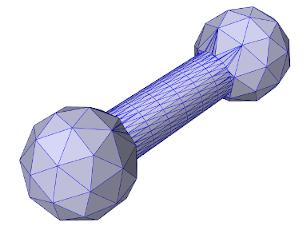
\includegraphics[]{images/dumbbellMeshUnion}
\else
 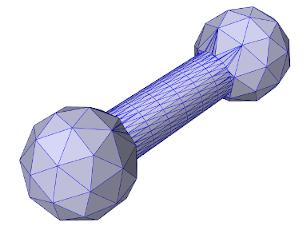
\includegraphics[width=3in]{images/dumbbellMeshUnion}
\fi
\end{center}
\caption{Dumbbell shaped mesh produced from the CSG union of
two balls and a cylinder.}
\label{dumbbellMeshUnion:fig}
\end{figure}

The CSG operations include union, intersection, and difference, and
are implemented by the following methods of {\tt SurfaceMeshIntersector}:
% method table
\begin{lstlisting}[]
  findUnion (mesh0, mesh1);         // volume0 U volume1
  findIntersection (mesh0, mesh1);  // volume0 ^ volume1
  findDifference01 (mesh0, mesh1);  // volume0 - volume1 
  findDifference10 (mesh0, mesh1);  // volume1 - volume0 
\end{lstlisting}
%
Each takes two {\tt PolyhedralMesh} objects, {\tt mesh0} and {\tt
mesh1}, and creates and returns another {\tt PolyhedralMesh} which
represents the boundary surface of the requested operation. If the
result of the operation is {\tt null}, the returned mesh will be empty.

The example below uses {\tt findUnion} to create a dumbbell shaped mesh
from two balls and a cylinder:
%
\begin{lstlisting}[]
  // first create two ball meshes and a bar mesh
  double radius = 1.0;
  int division = 1; // number of divisons for icosahedral sphere
  PolygonalMesh ball0 = MeshFactory.createIcosahedralSphere (radius, division);
  ball0.transform (new RigidTransform3d (0, -2*radius, 0));
  PolygonalMesh ball1 = MeshFactory.createIcosahedralSphere (radius, division);
  ball1.transform (new RigidTransform3d (0, 2*radius, 0));
  PolygonalMesh bar = MeshFactory.createCylinder (
     radius/2, radius*4, /*ns=*/32, /*nr=*/1, /*nh*/10);
  bar.transform (new RigidTransform3d (0, 0, 0, 0, 0, Math.PI/2));

  // use a SurfaceMeshIntersector to create a CSG union of these meshes
  SurfaceMeshIntersector smi = new SurfaceMeshIntersector();
  PolygonalMesh balls = smi.findUnion (ball0, ball1);
  PolygonalMesh mesh = smi.findUnion (balls, bar);
\end{lstlisting}
%
The balls and cylinder are created using the
\javaclass[\mgeo]{MeshFactory} methods
\javamethod*[\mgeo.MeshFactory]{createIcosahedralSphere(double,int)}
and
\javamethod*[\mgeo.MeshFactory]{createCylinder(double,double,int,int,int)},
where the latter takes arguments {\tt ns}, {\tt nr}, and {\tt nh}
giving the number of slices along the circumference, end-cap radius,
and length. The final resulting mesh is shown in Figure
\ref{dumbbellMeshUnion:fig}.

%\section{Geometric Queries}
%\label{GeometricQueries:sec}
%
%XXX

\section{Reading source relative files}
\label{PathFinder:sec}

ArtiSynth applications frequently need to read in various kinds of
data files, including mesh files (as discussed in Section
\ref{MeshFileIO:sec}), FEM mesh geometry (Section
\ref{FemGeometryFiles:sec}), probe data (Section
\ref{DataFileFormat:sec}), and custom application data.

Often these data files do not reside in an absolute location but
instead in a location relative to the application's class or source
files.  For example, it is common for applications to store geometric
data in a subdirectory {\tt "geometry"} located beneath the source
directory. In order to access such files in a robust way, and ensure
that the code does not break when the source tree is moved, it is
useful to determine the application's source (or class) directory at
run time. ArtiSynth supplies several ways to conveniently handle this
situation. First, the {\tt RootModel} itself supplies the following
methods:
% method table
\begin{lstlisting}[]
  // find path to the root model's source directory
  String findSourceDir ();

  // get path to a file specified relative to the root model's source directory
  String getSourceRelativePath (String relpath);
\end{lstlisting}
%
The first method returns the path to the source directory of the
root model, while the second returns the path to a file specified
relative to the root model source directory. If the root model source
directory cannot be found (see discussion at the end of this section)
both methods return {\tt null}.
%
As a specific usage example, assume that we have an application model
whose {\tt build()} method needs to load in a mesh {\tt torus.obj}
from a subdirectory {\tt meshes} located beneath the source
directory. This could be done as follows:
%
\begin{lstlisting}[]
  String pathToMesh = getSourceRelativePath ("meshes/torus.obj");
  // read the mesh from a .obj file :
  WavefrontReader reader = new WavefrontReader (pathToMesh);
  PolygonalMesh mesh = null;
  try {
     mesh = reader.readMesh () ;
  }
  catch (IOException e) {
     System.err.println ("Can't read mesh:");
     e.printStackTrace () ;
  }
\end{lstlisting}

A more general path finding utility is provided by
\javaclass{maspack.util.PathFinder}, which provides several static
methods for locating source and class directories:
% method table
\begin{lstlisting}[]
  // find path to the source directory associated with classObj
  String findSourceDir (Object classObj);

  // get path to a file specified relative to classObj source directory
  String getSourceRelativePath (Object classObj, String relpath);

  // find path to the class directory associated with classObj
  String findClassDir (Object classObj);

  // get path to a file specified relative to classObj class directory
  String getClassRelativePath (Object classObj, String relpath);
\end{lstlisting}
%
The ``find'' methods return a string path to the indicated class or
source directory, while the ``relative path'' methods locate the class
or source directory and append
the additional path {\tt relpath}.  For all of these, the class is
determined from {\tt classObj}, either directly (if it is an instance
of {\tt Class}), by name (if it is a {\tt String}), or otherwise by
calling {\tt classObj.getClass()}. When identifying a package by name,
the name should be either a fully qualified class name, or a simple
name that can be located with respect to the packages obtained via
{\tt Package.getPackages()}. For example, if we have a class whose
fully qualified name is {\tt artisynth.models.test.Foo}, then the
following calls should all return the same result:
%
\begin{lstlisting}[]
   Foo foo = new Foo();

   PathFinder.findSourceDir (foo);
   PathFinder.findSourceDir (Foo.class);
   PathFinder.findSourceDir ("artisynth.models.test.Foo");
   PathFinder.findSourceDir ("Foo");
\end{lstlisting}
%
If the source directory for {\tt Foo} happens to be {\tt
/home/projects/src/artisynth/models/test}, then
%
\begin{lstlisting}[]
   PathFinder.getSourceRelativePath (foo, "geometry/mesh.obj");
\end{lstlisting}
%
will return
{\tt /home/projects/src/artisynth/models/test/geometry/mesh.obj}.

\begin{sideblock}
When calling {\tt PathFinder} methods from {\it within} the relevant
class, one can specify {\tt this} as the {\tt classObj} argument.
\end{sideblock}

With respect to the above example locating the file {\tt
"meshes/torus.obj"}, the call to the root model method 
{\tt getSourceRelativePath()} could be replaced with
%
\begin{lstlisting}[]
  String pathToMesh = PathFinder.getSourceRelativePath (
     this, "meshes/torus.obj");
\end{lstlisting}
Since this is assumed to be called from the root model's build method,
the ``class'' can be indicated by simply passing {\tt this} to {\tt
getSourceRelativePath()}.

\begin{sideblock}
As an alternative to placing data files in the source directory, one
could place them in the class directory, and then use {\tt
findClassDir()} and {\tt getClassRelativePath()}. If the data files
were originally defined in the source directory, it will be necessary
to copy them to the class directory. Some Java IDEs will perform this
automatically.
\end{sideblock}

The {\tt PathFinder} methods work by climbing the class's resource
hierarchy.  Source directories are assumed to be located relative to
the parent of the root class directory, via one of the paths specified
by \javamethod[maspack.util.PathFinder]{getSourceRootPaths()}. By default, this
list includes {\tt "src"}, {\tt "source"}, and {\tt "bin"}. Additional
paths can be added using
\javamethodAlt{maspack.util.PathFinder.addSourceRootPath()}%
{addSourceRootPath(path)},
or the entire list can be set using
\javamethodAlt{maspack.util.PathFinder.setSourceRootPaths()}%
{setSourceRootPaths(paths)}.

At preset, source directories will not be found if the reference class
is contained in a jar file.

\section{Reading and caching remote files}
\label{FileManager:sec}

ArtiSynth applications often require the use of large data files to
specify items such as FEM mesh geometry, surface mesh geometry, or
medical imaging data. The size of these files may make it inconvenient
to store them in any version control system that is used to
store the application source code. As an alternative, ArtiSynth
provides a {\it file manager} utility that allows such files to be
stored on a separate server, and then downloaded on-demand and cached
locally. To use this, one starts by creating an instance of a
\javaclass[maspack.fileutil]{FileManager}, using the constructor
% method def
\begin{lstlisting}[]
  FileManager (String downloadPath, String remoteSourceName)
\end{lstlisting}
%
where {\tt downloadPath} is a path to the local directory where the
downloaded file should be placed, and {\tt remoteSourceName} is a URI
indicating the remote server location of the files.  After the file
manager has been created, it can be used to fetch remote files and
cache them locally, using various {\it get} methods:
% methd table
\begin{lstlisting}[]
  File get (String destName);

  File get (String destName, String sourceName);
\end{lstlisting}
%
Both of these look for the file {\tt destName} specified relative to
the local directory, and return a {\tt File} handle for it if it is
present. Otherwise, they attempt to download the file from the remote
source location, place it in the local directory, and return a {\tt
File} handle for it.
The location of the remote file is given relative to
the remote source URI by {\tt destName} for the first method and {\tt
sourceName} for the second.

A simple example of using a file manager within a {\tt RootModel} {\tt
build()} method is given by the following fragment:
%
\begin{lstlisting}[]
  // create the file manager ...
  FileManager fm = new FileManager (
    getSourceRelativePath("geometry"), 
    "http://myserver.org/artisynth/data/geometry");
  // ... and use it to get a bone mesh file
  File meshFile = fm.get ("tibia.obj");
\end{lstlisting}
%
Here, a file manager is created that uses a local directory {\tt "geometry"},
located relative to the {\tt RootModel} source directory (see Section
\ref{PathFinder:sec}), and looks for missing files relative to the URI
%
\begin{verbatim}
  http://myserver.org/artisynth/data/geometry
\end{verbatim}
%
The {\tt get()} method is then used to obtain the file {\tt
"tibia.obj"} from the local directory. If it is not already present,
it is downloaded from the remote location.

The \javaclass[maspack.fileutil]{FileManager} contains other features
and functionality, and one should consult its API documentation for
more information.

\ifdefined\maindoc
\else
\end{document}
\fi

\ifdefined\maindoc\else
% typesetting this chapter as a standalone document
\def\doctitle{Mechanical Models I}
% starting definitions for both the main document and stand-alone chapters
\documentclass{book}

\def\mech{artisynth.core.mechmodels}
\def\mgeo{maspack.geometry}

% Add search paths for input files
\makeatletter
\def\input@path{{../}{../../}{../texinputs/}}
\makeatother

\usepackage{amsmath}
\usepackage{framed}
%%
%% Default settings for artisynth
%%
\NeedsTeXFormat{LaTeX2e}
%%\ProvidesPackage{artisynthDoc}[2012/04/05]

\usepackage[T1]{fontenc}
\usepackage[latin1]{inputenc}
\usepackage{listings}
\usepackage{makeidx}
\usepackage{latexml}
\usepackage{graphicx}
\usepackage{framed}
\usepackage{booktabs}
\usepackage{color}

\newcommand{\pubdate}{\today}
\newcommand{\setpubdate}[1]{\renewcommand{\pubdate}{#1}}
\newcommand{\code}[1]{{\tt #1}}

\iflatexml
\usepackage{hyperref}
\setlength\parindent{0pt} 
\else
%% then we are making a PDF, so include things that LaTeXML can't handle: 
%% docbook style, \RaggedRight
\usepackage{ifxetex}
\usepackage{xstring}
\usepackage{pslatex} % fixes fonts; in particular sets a better-fitting \tt font

\usepackage[most]{tcolorbox}
\definecolor{shadecolor}{rgb}{0.95,0.95,0.95}
\tcbset{
    frame code={}
    center title,
    left=0pt,
    right=0pt,
    top=0pt,
    bottom=0pt,
    colback=shadecolor,
    colframe=white,
    width=\dimexpr\textwidth\relax,
    enlarge left by=0mm,
    boxsep=0pt,
    arc=0pt,outer arc=0pt,
}%

\usepackage[A4]{artisynth_papersize}
%\usepackage[letter]{artisynth_papersize}
\usepackage[hyperlink]{asciidoc-dblatex} 

%\usepackage{verbatim}
\usepackage{ragged2e}
\setlength{\RaggedRightRightskip}{0pt plus 4em}
\RaggedRight
\renewcommand{\DBKpubdate}{\pubdate}
\renewcommand{\DBKreleaseinfo}{}
\fi

% set hypertext links to be dark blue:
\definecolor{darkblue}{rgb}{0,0,0.8}
\definecolor{sidebar}{rgb}{0.5,0.5,0.7}
\hypersetup{colorlinks=true,urlcolor=darkblue,linkcolor=darkblue,breaklinks=true}

%%%%%%%%%%%%%%%%%%%%%%%%%%%%%%%%%%%%%%%%%%%%%%%%%%%%%%%%%%%%%%%%%%%%%%%%%%%%%
%
% Define macros for handling javadoc class and method references
%
%%%%%%%%%%%%%%%%%%%%%%%%%%%%%%%%%%%%%%%%%%%%%%%%%%%%%%%%%%%%%%%%%%%%%%%%%%%%%
\makeatletter

% macro to enable line break if inside a PDF file
\def\pdfbreak{\iflatexml\else\\\fi}

% code inspired by http://stackoverflow.com/questions/2457780/latex-apply-an-operation-to-every-character-in-a-string
\def\removeargs #1{\doremoveargs#1$\wholeString\unskip}
\def\doremoveargs#1#2\wholeString{\if#1$%
\else\if#1({()}\else{#1}\taketherest#2\fi\fi}
\def\taketherest#1\fi
{\fi \doremoveargs#1\wholeString}

% Note: still doesn't work properly when called on macro output ...
% i.e., \dottoslash{\concatnames{model}{base}{foo}} fails 
\def\dottoslash #1{\dodottoslash#1$\wholeString\unskip}
\def\dodottoslash#1#2\wholeString{\if#1$%
\else\if#1.{/}\else{#1}\fi\dottaketherest#2\fi}
\def\dottaketherest#1\fi{\fi \dodottoslash#1\wholeString}

\def\hashtodot #1{\dohashtodot#1$\wholeString\unskip}
\def\dohashtodot#1#2\wholeString{\if#1$X%
\else\if#1\#{.}\else{#1}\fi\hashtaketherest#2\fi}
\def\hashtaketherest#1\fi{\fi \dohashtodot#1\wholeString}

%\dollartodot{#1} does the same thing as \StrSubstitute[0]{#1}{\$}{.}
% from the packahe xstring. We define \dollartodot instead because
% LaTeXML does not implement xstring.
%
% Note that for the substituion to work, we need \ifx instead of \if,
% since otherwise escaped characters won't work properly:
% if #1 = \$, then \if#1* seems to compare '\' and '$' (and output '*'),
% rather than comparing '$' to '*'
\def\dollartodot #1{\dodollartodot#1*\wholeString\unskip}
\def\dodollartodot#1#2\wholeString{\ifx#1*%
\else \ifx#1\${.}\else{#1}\fi\dollartaketherest#2\fi}
\def\dollartaketherest#1\fi{\fi \dodollartodot#1\wholeString}

% concatenates up to three class/method names together, adding '.' characters
% between them. The first and/or second argument may be empty, in which case
% the '.' is omitted. To check to see if these arguments are empty, we
% use a contruction '\if#1@@', which will return true iff #1 is empty
% (on the assumption that #1 will not contain a '@' character).
\def\concatnames
#1#2#3{\if#1@@\if#2@@#3\else #2.#3\fi\else\if#2@@#1.#3\else#1.#2.#3\fi\fi}

\newcommand{\javabase}{}
\newcommand{\setjavabase}[1]{\renewcommand{\javabase}{#1}}

\def\artisynthDocBase{@ARTISYNTHDOCBASE}

\iflatexml
\def\ifempty#1{\def\temp{#1}\ifx\temp\empty}%
\newcommand{\artisynthManual}[3][]{%
   \ifempty{#1}
      \href{@ARTISYNTHDOCBASE/#2/#2.html}{#3}%
    \else
      \href{@ARTISYNTHDOCBASE/#1/#2.html}{#3}%
    \fi
}
\else
\newcommand{\artisynthManual}[3][]{%
\href{https://www.artisynth.org/@ARTISYNTHDOCBASE/#2.pdf}{#3}}
\fi

%\href{@ARTISYNTHDOCBASE/#2/#2.html}{#3}}



\newcommand{\javaclassx}[2][]{%
% Includes code to prevent an extra '.' at the front if #1 is empty. It
% works like this: if '#1' is empty, then '#1.' expands to '.', and so 
% '\if#1..' will return true, in which case we just output '#2'.
\href{@JDOCBEGIN/\concatnames{\javabase}{#1}{#2}@JDOCEND}{#2}}
\newcommand{\javaclass}[2][]{%
\href{@JDOCBEGIN/\concatnames{}{#1}{#2}@JDOCEND}{\dollartodot{#2}}}
\newcommand{\javaclassAlt}[2]{%
\href{@JDOCBEGIN/\concatnames{}{}{#1}@JDOCEND}{#2}}

\newcommand{\javamethodArgsx}[2][]{%
\href{@JDOCBEGIN/\concatnames{\javabase}{#1}{#2}@JDOCEND}{#2}}
\newcommand{\javamethodArgs}[2][]{%
\href{@JDOCBEGIN/\concatnames{}{#1}{#2}@JDOCEND}{#2}}
\newcommand{\javamethodAlt}[2]{%
\href{@JDOCBEGIN/\concatnames{}{}{#1}@JDOCEND}{#2}}
\newcommand{\javamethodAltx}[2]{%
\href{@JDOCBEGIN/\concatnames{\javabase}{}{#1}@JDOCEND}{#2}}

\newcommand{\javamethodNoArgsx}[2][]{%
\href{@JDOCBEGIN/\concatnames{\javabase}{#1}{#2}@JDOCEND}{\removeargs{#2}}}
\newcommand{\javamethodNoArgs}[2][]{%
\href{@JDOCBEGIN/\concatnames{}{#1}{#2}@JDOCEND}{\removeargs{#2}}}

\newcommand{\javamethod}{\@ifstar\javamethodNoArgs\javamethodArgs}
\newcommand{\javamethodx}{\@ifstar\javamethodNoArgsx\javamethodArgsx}

%%%%%%%%%%%%%%%%%%%%%%%%%%%%%%%%%%%%%%%%%%%%%%%%%%%%%%%%%%%%%%%%%%%%%%%%%%%%%
%
% Define macros for sidebars
%
%%%%%%%%%%%%%%%%%%%%%%%%%%%%%%%%%%%%%%%%%%%%%%%%%%%%%%%%%%%%%%%%%%%%%%%%%%%%%

\iflatexml
\newenvironment{sideblock}{\begin{quote}}{\end{quote}}
\else
\usepackage[strict]{changepage}
\definecolor{sidebarshade}{rgb}{1.0,0.97,0.8}
\newenvironment{sideblock}{%
    \def\FrameCommand{%
    \hspace{1pt}%
    {\color{sidebar}\vrule width 2pt}%
    %{\vrule width 2pt}%
    {\color{sidebarshade}\vrule width 4pt}%
    \colorbox{sidebarshade}%
  }%
  \MakeFramed{\advance\hsize-\width\FrameRestore}%
  \noindent\hspace{-4.55pt}% disable indenting first paragraph
  \begin{adjustwidth}{}{7pt}%
  %\vspace{2pt}\vspace{2pt}%
}
{%
  \vspace{2pt}\end{adjustwidth}\endMakeFramed%
}
\fi

\iflatexml
\newenvironment{shadedregion}{%
  \definecolor{shadecolor}{rgb}{0.96,0.96,0.98}%
  \begin{shaded*}%
% Put text inside a quote to create a surrounding blockquote that
% will properly accept the color and padding attributes
  \begin{quote}%
}
{%
  \end{quote}%
  \end{shaded*}%
}
\else
\newenvironment{shadedregion}{%
  \definecolor{shadecolor}{rgb}{0.96,0.96,0.98}%
  \begin{shaded*}%
}
{%
  \end{shaded*}%
}
\fi

% Wanted to create a 'listing' environment because lstlisting is
% tedious to type and because under latexml it may need
% some massaging to get it to work properly. But hard to do
% because of the verbatim nature of listing
%\iflatexml
%\newenvironment{listing}{\begin{lstlisting}}{\end{lstlisting}}%
%\else
%\newenvironment{listing}{\begin{lstlisting}}{\end{lstlisting}}%
%\fi

\iflatexml\else
% fancyhdr was complaining that it wanted a 36pt header height ...
\setlength{\headheight}{36pt}
\fi

% macro for backslash character
\newcommand\BKS{\textbackslash}

% macro for double hyphen (to prevent conversion of -- into -)
\newcommand\DHY{-{}-}

% Convenience stuff
\newcommand{\ifLaTeXMLelse}[2]{%
  \iflatexml %
  #1 %
  \else %
  #2 %
  \fi %
}

\newcommand{\ifLaTeXML}[1]{ %
  \iflatexml %
  #1 %
  \fi %
}

% new methodtable environment for documenting methods

% base width of the method table
\newlength{\methodtablewidth}
\iflatexml
\setlength{\methodtablewidth}{1.4\textwidth}
\else
\setlength{\methodtablewidth}{0.94\textwidth}
\fi
% horizontal space added at end of call to \methodentry
\newlength{\methodskip}
\setlength{\methodskip}{0pt}
% lengths set inside methodtable environment:
\newlength{\methodsiglength} % length of the method signature
\newlength{\methodcomlength} % length of the method comment
\setlength{\methodsiglength}{0.5\methodtablewidth}
\setlength{\methodcomlength}{0.5\methodtablewidth}

% command to add a method to a method table:
% arg #1: package and signature for finding URL
% arg #2: anchor text
% arg #3: comment describing the method
\newcommand{\methodentry}[3]{%
\javamethodAlt{#1}{\parbox[t]{\methodsiglength}{#2}}&
{\parbox[t]{\methodcomlength}{#3}}\\%
\noalign{\vspace{\methodskip}}}

% methodtable environment takes two arguments, both scale factors for
% methodtablewidth:
% arg #1: width of the method signature column
% arg #2: width of the method comment column
\newenvironment{methodtable}[3][0pt]{%
\begingroup
\setlength{\topskip}{0pt}
\setlength{\methodskip}{#1}
\setlength{\methodsiglength}{#2\methodtablewidth}%
\setlength{\methodcomlength}{#3\methodtablewidth}%
\iflatexml
\begin{snugshade}
\else
\begin{tcolorbox}
\fi
\renewcommand{\arraystretch}{1}
\begin{tabular}{ll}}{%
\end{tabular}
\renewcommand{\arraystretch}{1}
\iflatexml
\end{snugshade}
\else
\end{tcolorbox}
\fi
\endgroup}

% commands for added top, mid and bottom lines in the table.
% uses booktabs for PDF, regular hline for HTML
\newcommand{\topline}{\iflatexml\hline\else\toprule\fi}
\newcommand{\midline}{\iflatexml\hline\else\midrule\fi}
\newcommand{\botline}{\iflatexml\hline\else\bottomrule\fi}
\newcommand{\blankline}{%
\multicolumn{2}{l}{\iflatexml{@SPACE}\else\phantom{M}\fi}\\}%
% add vertical space within a two colum method environment
\newcommand{\methodspace}[1]{%
\iflatexml
\multicolumn{2}{l}{@VERTSPACE[#1]}\\
\else
\noalign{\vspace{#1}}%
\fi}%
% break a line and add an indentation of 1em
\newcommand{\brh}{\\\phantom{M}}

\makeatother

\def\matl{\left(\begin{matrix}}
\def\matr{\end{matrix}\right)}

\def\Bthe{\boldsymbol\theta}
\def\Btau{\boldsymbol\tau}
\def\Bom{\boldsymbol\omega}
\def\Bdel{\boldsymbol\delta}
\def\Blam{\boldsymbol\lambda}
\def\Bphi{\boldsymbol\phi}
\def\Bxi{\boldsymbol\xi}
\def\Bgam{\boldsymbol\gamma}
\def\Bsig{\boldsymbol\sigma}
\def\Bnu{\boldsymbol\nu}
\def\Bmu{\boldsymbol\mu}

\def\A{{\bf A}}
\def\B{{\bf B}}
\def\C{{\bf C}}
\def\D{{\bf D}}
\def\F{{\bf F}}
\def\G{{\bf G}}
\def\H{{\bf H}}
\def\I{{\bf I}}
\def\J{{\bf J}}
\def\K{{\bf K}}
\def\Jc{{\bf J}_c}
\def\L{{\bf L}}
\def\M{{\bf M}}
\def\N{{\bf N}}
\def\O{{\bf O}}
\def\P{{\bf P}}
\def\Q{{\bf Q}}
\def\R{{\bf R}}
\def\T{{\bf T}}
\def\U{{\bf U}}
\def\W{{\bf W}}
\def\X{{\bf X}}
\def\Minv{{\bf M}^{-1}}

\def\a{{\bf a}}
\def\b{{\bf b}}
\def\c{{\bf c}}
\def\d{{\bf d}}
\def\e{{\bf e}}
\def\f{{\bf f}}
\def\g{{\bf g}}
\def\k{{\bf k}}
\def\l{{\bf l}}
\def\m{{\bf m}}
\def\n{{\bf n}}
\def\p{{\bf p}}
\def\q{{\bf q}}
\def\r{{\bf r}}
\def\u{{\bf u}}
\def\v{{\bf v}}
\def\w{{\bf w}}
\def\x{{\bf x}}
\def\y{{\bf y}}
\def\z{{\bf z}}

\def\ma{{\bf m}_\alpha}
\def\mb{{\bf m}_\beta}
\def\va{{\bf v}_\alpha}
\def\vb{{\bf v}_\beta}
\def\vp{{\bf v}_\rho}
\def\vk{{\bf v}_k}
\def\ua{{\bf u}_\alpha}
\def\ub{{\bf u}_\beta}
\def\uk{{\bf u}_k}
\def\uj{{\bf u}_j}
\def\mar{{\bf m}_{\alpha r}}
\def\mbr{{\bf m}_{\beta r}}

\def\Maa{{\bf M}_{\alpha\alpha}}
\def\Mab{{\bf M}_{\alpha\beta}}
\def\Mba{{\bf M}_{\beta\alpha}}
\def\Mbb{{\bf M}_{\beta\beta}}
\def\hatMaa{\hat{\bf M}_{\alpha\alpha}}
\def\hatMab{\hat{\bf M}_{\alpha\beta}}
\def\hatMba{\hat{\bf M}_{\beta\alpha}}
\def\hatMbb{\hat{\bf M}_{\beta\beta}}
\def\Mbp{{\bf M}_{\beta\rho}}
\def\Map{{\bf M}_{\alpha\rho}}
\def\Mpa{{\bf M}_{\rho\alpha}}
\def\Mpb{{\bf M}_{\rho\beta}}
\def\Mpp{{\bf M}_{\rho\rho}}
\def\Mbk{{\bf M}_{\beta k}}
\def\Mak{{\bf M}_{\alpha k}}
\def\Mka{{\bf M}_{k\alpha}}
\def\Mkb{{\bf M}_{k\beta}}
\def\Mkk{{\bf M}_{kk}}

\def\Ga{{\bf G}_{\alpha}}
\def\Gp{{\bf G}_{\rho}}
\def\Gaa{{\bf G}_{\alpha\alpha}}
\def\Gab{{\bf G}_{\alpha\beta}}
\def\Gba{{\bf G}_{\beta\alpha}}
\def\Gbb{{\bf G}_{\beta\beta}}
\def\Gap{{\bf G}_{\alpha\rho}}
\def\Gpa{{\bf G}_{\rho\alpha}}
\def\Gbp{{\bf G}_{\beta\rho}}
\def\Gak{{\bf G}_{\alpha k}}
\def\Gka{{\bf G}_{k\alpha}}
\def\Gja{{\bf G}_{j\alpha}}
\def\Gkb{{\bf G}_{k\beta}}
\def\Gbk{{\bf G}_{\beta k}}

\def\lama{\Blam_{\alpha}}
\def\lamb{\Blam_{\beta}}
\def\lamp{\Blam_{\rho}}
\def\lamk{\Blam_{k}}
\def\lams{\Blam_{\sigma}}

\def\ba{{\bf b}_{\alpha}}
\def\bb{{\bf b}_{\beta}}
\def\fp{{\bf f}_{\rho}}
\def\fa{{\bf f}_{\alpha}}
\def\qa{{\bf q}_{\alpha}}
\def\qb{{\bf q}_{\beta}}
\def\za{{\bf z}_{\alpha}}
\def\zb{{\bf z}_{\beta}}
\def\wa{{\bf w}_{\alpha}}
\def\wb{{\bf w}_{\beta}}

\def\Na{\bar{\bf N}_{\alpha}}
\def\Nb{\bar{\bf N}_{\beta}}

\def\Up{{\bf U}_p}
\def\Un{{\bf U}_n}

\def\dFdl{\frac{\partial F}{\partial l}}
\def\dFddl{\frac{\partial F}{\partial \dot l}}

\def\Sr{s_\theta}
\def\Cr{c_\theta}
\def\Sp{s_\phi}
\def\Cp{c_\phi}
\def\Sy{s_\psi}
\def\Cy{c_\psi}
\def\Sa{s_{\alpha}}
\def\Ca{c_{\alpha}}
\def\Vp{v_{\phi}}


\iflatexml
\else
\usepackage{biblatex}
\addbibresource{references.bib}
\fi

\setcounter{tocdepth}{5}
\setcounter{secnumdepth}{3}

\title{\doctitle}
\ifdefined\maindoc
\author{John Lloyd and Antonio S\'anchez}
\setpubdate{Last update: March, 2022}

\iflatexml
\date{}
\fi
\fi

% graphics paths
\graphicspath{{./}{images/}}

% Listings settings
\definecolor{myblue}{rgb}{0,0,0.6}
\definecolor{mygreen}{rgb}{0,0.6,0}
\definecolor{mygray}{rgb}{0.5,0.5,0.5}
\definecolor{mylightgray}{rgb}{0.95,0.95,0.95}
\definecolor{mymauve}{rgb}{0.58,0,0.82}
\definecolor{myblack}{rgb}{0,0,0}
\lstset{
   language=Java,                   % text highlighting for Java
   breakatwhitespace=false,         % automatic breaks only at whitespace
   breaklines=true,                 % automatic line breaking
   commentstyle=\color{mygreen},    % comment style
   keepspaces=true,                 % keeps spaces in text
   keywordstyle=\color{myblue},     % keyword style
   numbers=none,                    % line-numbers; values: (none, left, right)
   numbersep=5pt,                   % how far the line-numbers are from code
   numberstyle=\tiny\color{mygray}, % line-numbers style
   showspaces=false,                % show spaces everywhere
   showstringspaces=false,          % underline spaces within strings
   showtabs=false,                  % show tabs
   stepnumber=1,                    % the step between two line-numbers
   stringstyle=\color{mymauve},     % string literal style
   tabsize=3,                       % sets default tabsize to 3 spaces
   backgroundcolor=\color{mylightgray}, % background color
   frame=single, 					% adds a frame around the code
   rulesepcolor=\color{mygray},
   rulecolor=\color{myblack},
   framerule=0pt,
   xleftmargin=2.2ex,               % numbers inside box
   framexleftmargin=2.2ex,			% indentation of frame
}

\begin{document}

\frontmatter

%\layout
\maketitle

\iflatexml{\large\pubdate}\fi

\tableofcontents

\mainmatter
\fi

\chapter{Mechanical Models I}
\label{MechModelsI:sec}

This section details how to build basic multibody-type mechanical
models consisting of particles, springs, rigid bodies, joints, and
other constraints.

\section{Springs and particles}
\label{ParticlesAndSprings:sec}

The most basic type of mechanical model consists simply of particles
connected together by axial springs.  Particles are implemented by the
class \javaclass[artisynth.core.mechmodels]{Particle}, which is a
dynamic component containing a three-dimensional position state, a
corresponding velocity state, and a mass. It is an instance of the
more general base class \javaclass[artisynth.core.mechmodels]{Point},
which is used to also implement spatial points such as {\tt markers}
which do not have a mass.

\subsection{Axial springs and materials}
\label{AxialSprings:sec}

An axial spring is a simple spring that connects two points and is
implemented by the class
\javaclass[artisynth.core.mechmodels]{AxialSpring}. This is a {\it
force effector} component that exerts equal and opposite forces on the
two points, along the line separating them, with a magnitude $f$ that
is a function $f(l, \dot l)$ of the distance $l$ between the points,
and the distance derivative $\dot l$.

Each axial spring is associated with an {\it axial material},
implemented by a subclass of
\javaclass[artisynth.core.materials]{AxialMaterial}, that specifies
the function $f(l, \dot l)$. The most basic type of axial material is
a \javaclass[artisynth.core.materials]{LinearAxialMaterial}, which
determines $f$ according to the linear relationship
%
\begin{equation}
f(l, \dot l) = k (l-l_0) + d \dot l
\end{equation}
%
where $l_0$ is the rest length and $k$ and $d$ are the stiffness and
damping terms. Both $k$ and $d$ are properties of the material, while
$l_0$ is a property of the spring.

Axial springs are assigned a linear axial material by default.  More
complex, nonlinear axial materials may be defined in the package {\tt
artisynth.core.materials}. Setting or querying a spring's material
may be done with the methods {\tt setMaterial()} and {\tt
getMaterial()}.

\subsection{Example: a simple particle-spring model}
\label{ParticleSpringExample:sec}

\begin{figure}[t]
\begin{center}
\iflatexml
 \includegraphics[]{images/ParticleSpring}
\else
 \includegraphics[width=3.75in]{images/ParticleSpring}
\fi
\end{center}
\caption{ParticleSpring model loaded into ArtiSynth.}
\label{ParticleSpring:fig}
\end{figure}

An complete application model that implements a simple particle-spring
model is given below. 
\lstset{numbers=left}
\lstinputlisting{../../src/artisynth/demos/tutorial/ParticleSpring.java}
\lstset{numbers=none}

Line 1 of the source defines the package in which the model class will
reside, in this case {\tt artisynth.demos.tutorial}. Lines 3-8 import
definitions for other classes that will be used.

The model application class is named {\tt ParticleSpring} and declared
to extend {\tt RootModel} (line 13), and the {\tt build()} method
definition begins at line 15. (A no-args constructor is also needed,
but because no other constructors are defined, the compiler creates
one automatically.)

To begin, the {\tt build()} method creates a {\tt MechModel} named
{\tt "mech"}, and then adds it to the {\tt models} list of the root model
using the {\tt addModel()} method (lines 18-19). Next, two particles,
{\tt p1} and {\tt p2}, are created, with masses equal to 2 and initial
positions at 0, 0, 0, and 1, 0, 0, respectively (lines 22-23). Then an
axial spring is created, with end points set to {\tt p1} and {\tt p2},
and assigned a linear material with a stiffness and damping of 20 and
10 (lines 24-27). Finally, after the particles and the spring are
created, they are added to the {\tt particles} and {\tt axialSprings}
lists of the {\tt MechModel} using the methods {\tt
addParticle()} and {\tt addAxialSpring()} (lines 30-32).

At this point in the code, both particles are defined to be
dynamically controlled, so that running the simulation would cause
both to fall under the {\tt MechModel}'s default gravity acceleration
of $(0, 0, -9.8)$. However, for this example, we want the first
particle to remain fixed in place, so we set it to be {\it
non-dynamic} (line 34), meaning that the physical simulation will not
update its position in response to forces (Section
\ref{DynamicVsParametric:sec}).

The remaining calls control aspects of how the model is graphically
rendered.  {\tt setBounds()} (line 37) increases the model's
``bounding box'' so that by default it will occupy a larger part of
the viewer frustum. The convenience method {\tt
RenderProps.setSphericalPoints()} is used to set points {\tt p1} and
{\tt p2} to render as solid red spheres with a radius of 0.06, while
{\tt RenderProps.setCylindricalLines()} is used to set {\tt spring} to
render as a solid blue cylinder with a radius of 0.02. More details
about setting render properties are given in Section
\ref{RenderProperties:sec}.

To run this example in ArtiSynth, select {\sf All demos > tutorial >
ParticleSpring} from the {\sf Models} menu. The model should load and
initially appear as in Figure \ref{ParticleSpring:fig}.  Running
the model (Section \ref{LoadingAndRunning:sec}) will
cause the second particle to fall and swing about under gravity.

\subsection{Dynamic, parametric, and attached components}
\label{DynamicVsParametric:sec}

By default, a dynamic component is advanced through time in response
to the forces applied to it. However, it is also possible to set a
dynamic component's {\tt dynamic} property to {\tt false}, so that it
does not respond to force inputs.  As shown in the example above, this
can be done using the method
{\tt setDynamic()}:
%
\begin{verbatim}
  comp.setDynamic (false);
\end{verbatim}
%
The method
\javamethod*[artisynth.core.mechmodels.DynamicAgent]{isDynamic()}
can be used to query the {\tt dynamic} property.

Dynamic components can also be {\it attached} to other dynamic
components (as mentioned in Section \ref{PhysicsSimulation:sec}) so
that their positions and velocities are controlled by the {\it master}
components that they are attached to.  To attach a dynamic component,
one creates an {\tt AttachmentComponent} specifying the attachment
connection and adds it to the {\tt MechModel}, as described in Section
\ref{Attachments:sec}.  The method
\javamethod*[artisynth.core.mechmodels.DynamicAgent]{isAttached()}
can be used to determine if a component is attached, and if it is,
\javamethod*[artisynth.core.mechmodels.DynamicAgent]{getAttachment()}
can be used to find the corresponding {\tt AttachmentComponent}.

Overall, a dynamic component can be in one of three states:

\begin{description}

\item[active]\mbox{}

Component is dynamic and unattached. The method
\javamethod*[artisynth.core.mechmodels.DynamicAgent]{isActive()}
returns {\tt true}. The component will move in response to forces.

\item[parametric]\mbox{}

Component is not dynamic, and is unattached. 
The method
\javamethod*[artisynth.core.mechmodels.DynamicAgent]{isParametric()}
returns {\tt true}.
The component will either remain
fixed, or will move around in response to external inputs specifying
the component's position and/or velocity. One way to supply such
inputs is to use controllers or input probes, as described in
Section \ref{SimulationControl:sec}.

\item[attached]\mbox{}

Component is attached. The method
\javamethod*[artisynth.core.mechmodels.DynamicAgent]{isAttached()}
returns {\tt true}. The component will move so as to follow the other
master component(s) to which it is attached.

\end{description}

\subsection{Custom axial materials}
\label{CustomAxialMaterials:sec}

Application authors may create their
own axial materials by subclassing 
\javaclass[artisynth.core.materials]{AxialMaterial}
and overriding the functions
% method table
\begin{lstlisting}[]
  double computeF (l, ldot, l0, excitation);
  double computeDFdl (l, ldot, l0, excitation);
  double computeDFdldot (l, ldot, l0, excitation);
  boolean isDFdldotZero ();
\end{lstlisting}
%
where {\tt excitation} is an additional {\it excitation} signal $a$, which
is used to implement active springs and which in particular is used to
implement axial muscles (Section \ref{PointToPointMuscles:sec}), for
which $a$ is usually in the range $[0, 1]$.

The first three methods should return the values of 
%
\begin{equation}
f (l, \dot l, a), \quad
\frac{\partial f(l, \dot l, a)}{\partial l}, \quad \text{and} \quad
\frac{\partial f(l, \dot l, a)}{\partial \dot l},
\end{equation}
%
respectively, while the last method should return {\tt true} if
$\partial f(l, \dot l, a) / \partial \dot l \equiv 0$; i.e., if it is
always equals to 0.

\subsection{Damping parameters}

Mechanical models usually contain damping forces in addition to
spring-type restorative forces. Damping generates forces that reduce
dynamic component velocities, and is usually the major source of
energy dissipation in the model. Damping forces can be generated by
the spring components themselves, as described above.

A general damping can be set for all particles by setting the
{\tt MechModel}'s {\tt pointDamping} property. This causes
a force
%
\begin{equation}
\f_i = -d_p \v_i \label{eqn:pointdamping}
\end{equation}
%
to be applied to all particles, where $d_p$ is the value of the {\tt
pointDamping} and $\v_i$ is the particle's velocity.

{\tt pointDamping} can be set and queried using the {\tt MechModel}
methods
% method table
\begin{lstlisting}[]
  setPointDamping (double d);
  double getPointDamping();
\end{lstlisting}
%

\begin{sideblock}
In general, whenever a component has a property {\tt propX}, that
property can be set and queried in code using methods of the form
\begin{verbatim}
  setPropX (T d);
  T getPropX();
\end{verbatim}
where {\tt T} is the type associated with the property.
\end{sideblock}

{\tt pointDamping} can also be set for particles individually.  This
property is {\it inherited} (Section
\ref{CompositeInheritableProperties:sec}), so that if not set
explicitly, it inherits the nearest explicitly set value in an
ancestor component.

\section{Rigid bodies}

Rigid bodies are implemented in ArtiSynth by the class
\javaclass[artisynth.core.mechmodels]{RigidBody}, which is a dynamic
component containing a six-dimensional position and orientation state,
a corresponding velocity state, an inertia, and an optional surface
mesh.

A rigid body is associated with its own 3D spatial coordinate frame,
and is a subclass of the more general
\javaclass[artisynth.core.mechmodels]{Frame} component.
The combined position and orientation of this frame with respect to
world coordinates defines the body's {\it pose}, and the associated 6
degrees of freedom describe its ``position'' state.

\subsection{Frame markers}
\label{FrameMarkers:sec}

\begin{figure}[t]
\begin{center}
 \iflatexml
   \includegraphics[width=2.5in]{images/frameMarker}
 \else
   \includegraphics[width=2.5in]{images/frameMarker}
 \fi
\end{center}
\caption{A force $\f$ applied to a frame marker attached to a rigid
body. The marker is located at the point $\r$ with respect to the body
coordinate frame B.}
\label{frameMarker:fig}
\end{figure}

ArtiSynth makes extensive use of {\it markers}, which are (massless)
points attached to dynamic components in the model. Markers are used
for graphical display, implementing attachments, and transmitting
forces back onto the underlying dynamic components.

A {\it frame marker} is a marker that can be attached to a
\javaclass[artisynth.core.mechmodels]{Frame}, and most commonly to a
\javaclass[artisynth.core.mechmodels]{RigidBody} (Figure
\ref{frameMarker:fig}). They are frequently used to provide the
anchor points for attaching springs and, more generally, applying
forces to the body.

Frame markers are implemented by the class
\javaclass[artisynth.core.mechmodels]{FrameMarker}, which
is a subclass of
\javaclass[artisynth.core.mechmodels]{Point}.
The methods
% method table
\begin{lstlisting}[]
  Point3d getLocation();
  void setLocation (Point3d r);
\end{lstlisting}
%
get and set the marker's location $\r$ with respect to the frame's
coordinate system. When a 3D force $\f$ is applied to the marker, it
generates a spatial force $\hat\f$ (Section
\ref{SpatialVelocitiesAndForces:sec}) on the frame given by
%
\begin{equation}
\hat\f = \matl \f \\ \r \times \f \matr.
\end{equation}
%

Frame markers can be created using a variety of constructors, including
% method table
\begin{lstlisting}[]
  FrameMarker ();
  FrameMarker (String name);
  FrameMarker (Frame frame, Point3d loc);
\end{lstlisting}
%
where {\tt FrameMarker()} creates an empty marker, {\tt
FrameMarker(name)} creates an empty marker with a name, and {\tt
FrameMarker(frame,loc)} creates an unnamed marker attached to {\tt
frame} at the location {\tt loc} with respect to the frame's
coordinates. Once created, a marker's frame can be set and queried
with
% method table
\begin{lstlisting}[]
  void setFrame (Frame frame);
  Frame getFrame (); 
\end{lstlisting}
%
A frame marker can be added to a \javaclass[\mech]{MechModel} with the
{\tt MechModel} methods
% method table
\begin{lstlisting}[]
  void addFrameMarker (FrameMarker mkr);
  void addFrameMarker (FrameMarker mkr, Frame frame, Point3d loc);
\end{lstlisting}
%
where {\tt addFrameMarker(mkr,frame,loc)} also sets the frame and the
marker's location with respect to it. 

{\tt MechModel} also supplies convenience methods to create a
marker, attach it to a frame, and add it to the model:
% method table
\begin{lstlisting}[]
  FrameMarker addFrameMarker (Frame frame, Point3d loc);
  FrameMarker addFrameMarkerWorld (Frame frame, Point3d locw);
\end{lstlisting}
%
Both methods return the created marker. 
The first, {\tt addFrameMarker(frame,loc)}, places it at the
location {\tt loc} with respect to the frame, while {\tt
addFrameMarkerWorld(frame,pos)} places it at {\tt pos} with respect to
{\it world} coordinates.

\subsection{Example: a simple rigid body-spring model}
\label{RigidBodySpringExample:sec}

\begin{figure}[ht]
\begin{center}
\iflatexml
 \includegraphics[]{images/RigidBodySpring}
\else
 \includegraphics[width=3.75in]{images/RigidBodySpring}
\fi
\end{center}
\caption{RigidBodySpring model loaded into ArtiSynth.}
\label{RigidBodySpring:fig}
\end{figure}

A simple rigid body-spring model is defined in
%
\begin{verbatim}
  artisynth.demos.tutorial.RigidBodySpring
\end{verbatim}
%
This differs from ParticleSpring only in the {\tt build()} method,
which is listed below:
\lstset{numbers=left}
\begin{lstlisting}[]
   public void build (String[] args) {

      // create MechModel and add to RootModel
      MechModel mech = new MechModel ("mech");
      addModel (mech);

      // create the components
      Particle p1 = new Particle ("p1", /*mass=*/2, /*x,y,z=*/0, 0, 0);
      // create box and set its pose (position/orientation):
      RigidBody box =
         RigidBody.createBox ("box", /*wx,wy,wz=*/0.5, 0.3, 0.3, /*density=*/20);
      box.setPose (new RigidTransform3d (/*x,y,z=*/0.75, 0, 0));
      // create marker point and connect it to the box:
      FrameMarker mkr = new FrameMarker (/*x,y,z=*/-0.25, 0, 0);
      mkr.setFrame (box);

      AxialSpring spring = new AxialSpring ("spr", /*restLength=*/0);
      spring.setPoints (p1, mkr);
      spring.setMaterial (
         new LinearAxialMaterial (/*stiffness=*/20, /*damping=*/10));

      // add components to the mech model
      mech.addParticle (p1);
      mech.addRigidBody (box);
      mech.addFrameMarker (mkr);
      mech.addAxialSpring (spring);

      p1.setDynamic (false);               // first particle set to be fixed

      // increase model bounding box for the viewer
      mech.setBounds (/*min=*/-1, 0, -1, /*max=*/1, 0, 0);  
      // set render properties for the components
      RenderProps.setSphericalPoints (p1, 0.06, Color.RED);
      RenderProps.setSphericalPoints (mkr, 0.06, Color.RED);
      RenderProps.setCylindricalLines (mkr, 0.02, Color.BLUE);
   }
\end{lstlisting}
\lstset{numbers=none} 
The differences from {\tt ParticleSpring} begin
at line 9. Instead of creating a second particle, a rigid body is
created using the factory method
\javamethod*[artisynth.core.mechmodels]{RigidBody.createBox()}, which
takes x, y, z widths and a (uniform) density and creates a box-shaped
rigid body complete with surface mesh and appropriate mass and
inertia. As the box is initially centered at the origin, moving it
elsewhere requires setting the body's pose, which is done using {\tt
setPose()}. The {\tt RigidTransform3d} passed to {\tt setPose()} is
created using a three-argument constructor that generates a
translation-only transform.  Next, starting at line 14, a {\tt
FrameMarker} is created for a location $(-0.25, 0, 0)^T$ relative to the
rigid body, and attached to the body using its {\tt setFrame()}
method.

The remainder of {\tt build()} is the same as for {\tt ParticleSpring},
except that the spring is attached to the frame marker instead of a
second particle.

To run this example in ArtiSynth, select {\sf All demos > tutorial >
RigidBodySpring} from the {\sf Models} menu. The model should load and
initially appear as in Figure \ref{RigidBodySpring:fig}.  Running the
model (Section \ref{LoadingAndRunning:sec}) will cause the rigid body
to fall and swing about under gravity.

\subsection{Creating rigid bodies}

As illustrated above, rigid bodies can be created using factory
methods supplied by \javaclass[artisynth.core.mechmodels]{RigidBody}.
Some of these include:
% method table
\begin{lstlisting}[]
  createBox (name, widthx, widthy, widthz, density);
  createCylinder (name, radius, height, density, nsides);
  createSphere (name, radius, density, nslices);
  createEllipsoid (name, radx, rady, radz, density, nslices);
\end{lstlisting}
%
The bodies do not need to be named; if no name is desired, then {\tt
name} and can be specified as {\tt null}.

In addition, there are also
factory methods for creating a rigid body directly from a mesh:
% method table
\begin{lstlisting}[]
  createFromMesh (name, mesh, density, scale);
  createFromMesh (name, meshFileName, density, scale);
\end{lstlisting}
%
These take either a polygonal mesh (Section \ref{Meshes:sec}), or a
file name from which a mesh is read, and use it as the body's surface
mesh and then compute the mass and inertia properties from the specified
(uniform) density.

\begin{sideblock}
When a body is created directly from a surface mesh, its center of
mass will typically {\it not} be coincident with the origin of its
coordinate frame. Section \ref{RigidBodyCOM:sec} discusses the
implications of this and how to correct it.
\end{sideblock}

Alternatively, one can create a rigid body directly from a
constructor, and then set the mesh and inertia properties explicitly:
%
\begin{lstlisting}[]
  PolygonalMesh femurMesh;
  SpatialInertia inertia;

  ... initialize mesh and inertia appropriately ...

  RigidBody body = new RigidBody ("femur");
  body.setMesh (femurMesh);
  body.setInertia (inertia);
\end{lstlisting}
%

\subsection{Pose and velocity}

A body's pose can be set and
queried using the methods
% method table
\begin{lstlisting}[]
  setPose (RigidTransform3d T);   // sets the pose to T
  getPose (RigidTransform3d T);   // gets the current pose in T
  RigidTransform3d getPose();     // returns the current pose (read-only)
\end{lstlisting}
%
These use a \javaclass[maspack.matrix]{RigidTransform3d} (Section
\ref{RigidTransform3d:sec}) to describe the pose. Body poses are
described in world coordinates and specify the transform from body to
world coordinates. In particular, the pose for a body A specifies
the rigid transform $\T_{AW}$.

Rigid bodies also expose the translational and rotational components of
their pose via the properties {\tt position} and {\tt orientation},
which can be queried and set independently using the methods
% method table
\begin{lstlisting}[]
  setPosition (Point3d p);       // sets the position to p
  getPosition (Point3d p);       // gets the current position in p
  Point3d getPosition();         // returns the current position (read-only)

  setOrientation (AxisAngle a);  // sets the orientation to a
  getOrientation (AxisAngle a);  // gets the current orientation in a
  AxisAngle getOrientation();    // returns the current orientation (read-only)
\end{lstlisting}
%

The velocity of a rigid body is described using a
\javaclass[maspack.spatialmotion]{Twist} (Section
\ref{SpatialVectors:sec}), which contains both the translational and
rotational velocities. The following methods
set and query the spatial velocity as described with respect to world
coordinates:
% method table
\begin{lstlisting}[]
  setVelocity (Twist v);         // sets the spatial velocity to v
  getVelocity (Twist v);         // gets the current spatial velocity in v
  Twist getVelocity();           // returns current spatial velocity (read-only)
\end{lstlisting}
%

During simulation, unless a rigid body has been set to be {\it
parametric} (Section \ref{DynamicVsParametric:sec}), its pose and
velocity are updated in response to forces, so setting the pose or
velocity generally makes sense only for setting initial conditions.
On the other hand, if a rigid body is parametric, then it is possible
to control its pose during the simulation, but in that case it is
better to set its {\it target pose} and/or {\it target velocity}, as
described in Section \ref{ControllerImplementation:sec}.

\subsection{Inertia and the surface mesh}
\label{rigidBodyInertia:sec}

The ``mass'' of a rigid body is described by its spatial inertia,
which is a $6 \times 6$ matrix relating its spatial velocity to its
spatial momentum (Section \ref{SpatialInertia:sec}).  Within
ArtiSynth, spatial inertia is described by a
\javaclass[maspack.spatialmotion]{SpatialInertia} object, which
specifies its mass, center of mass (with respect to body coordinates),
and rotational inertia (with respect to the center of mass).

Most rigid bodies are also associated with a polygonal surface mesh,
which can be set and queried using the methods
% method table
\begin{lstlisting}[]
  setSurfaceMesh (PolygonalMesh mesh);
  setSurfaceMesh (PolygonalMesh mesh, String meshFileName);
  PolygonalMesh getSurfaceMesh();
\end{lstlisting}
%
The second method takes an optional {\tt fileName} argument that can
be set to the name of a file from which the mesh was read. Then if the
model itself is saved to a file, the model file will specify the mesh
using the file name instead of explicit vertex and face information,
which can reduce the model file size considerably.

Rigid bodies can also have more than one mesh, as described
in Section \ref{rigidBodyMultipleMeshes:sec}.

The inertia of a rigid body can be explicitly set using a variety
of methods including
% method table
\begin{lstlisting}[]
  setInertia (M)                    // set using SpatialInertia M
  setInertia (mass, Jxx, Jyy, Jzz); // mass and diagonal rotational inertia
  setInertia (mass, J);             // mass and full rotational inertia
  setInertia (mass, J, com);        // mass, rotational inertia, center-of-mass
\end{lstlisting}
%
and can be queried using 
% method table
\begin{lstlisting}[]
  getInertia (M);                   // get SpatialInertia in M
  getInertia ();                    // return read-only SpatialInertia
\end{lstlisting}
%

In practice, it is often more convenient to simply specify a mass or a
density, and then use the geometry of the surface mesh (and possibly
other meshes, Section \ref{rigidBodyMultipleMeshes:sec}) to compute
the remaining inertial values. How a rigid body's inertia is computed
is determined by its {\sf inertiaMethod} property, which can be one

\begin{description}

\item[EXPLICIT]\mbox{}

Inertia is set explicitly.

\item[MASS]\mbox{}

Inertia is determined implicitly from the mesh geometry and the body's
mass.

\item[DENSITY]\mbox{}

Inertia is determined implicitly from the mesh geometry and the body's
density (which is multiplied by the mesh volume(s) to determine a
mass).

\end{description}

\begin{sideblock}
When using {\tt DENSITY} to determine the inertia, it is generally
assumed that the contributing meshes are both polygonal and
closed. Meshes which are either open or non-polygonal generally do not
have a well-defined volume which can be multiplied by the density to
determine the mass.
\end{sideblock}

The {\sf inertiaMethod} property can be set and queried using
% method table
\begin{lstlisting}[]
  setInertiaMethod (InertiaMethod method);
  InertiaMethod getInertiaMethod();
\end{lstlisting}
%
and its default value is {\tt DENSITY}. Explicitly setting the
inertia using one of {\tt setInertia()} methods described above will
set {\tt inertiaMethod} to {\tt EXPLICIT}. The method
% method table
\begin{lstlisting}[]
  setInertiaFromDensity (density); 
\end{lstlisting}
%
will (re)compute the inertia using the mesh geometry and a density value
and set {\tt inertiaMethod} to {\tt DENSITY}, and
the method
% method table
\begin{lstlisting}[]
  setInertiaFromMass (mass); 
\end{lstlisting}
%
will (re)compute the inertia using the mesh geometry and a mass value
and set {\tt inertiaMethod} to {\tt MASS}.

Finally, the (assumed uniform) density of the body can be queried
using
% method table
\begin{lstlisting}[]
   getDensity();
\end{lstlisting}
%

\begin{sideblock}
There are some subtleties involved in determining the inertia using
either the {\tt DENSITY} or {\tt MASS} methods when the rigid body
contains more than one mesh. Details are given in Section
\ref{rigidBodyMultipleMeshes:sec}.
\end{sideblock}

\subsection{Coordinate frames and the center of mass}
\label{RigidBodyCOM:sec}

\begin{figure}[h]
\begin{center}
\iflatexml
 \includegraphics[width=3.75in]{images/RigidBodyCOM}
\else
 \includegraphics[width=3.75in]{images/RigidBodyCOM}
\fi
\end{center}
\caption{Left: rigid body whose coordinate frame B is not coincident
with the center of mass (COM). Right: same body, with its coordinate
frame translated to be coincident with the COM.}
\label{RigidBodyCOM:fig}
\end{figure}

It is important to note that the origin of a body's coordinate frame
will not necessarily coincide with its center of mass (COM), and in
fact the frame origin does not even have to lie inside the body's
surface (Figure \ref{RigidBodyCOM:fig}). This typically occurs when a
body's inertia is computed directly from its surface mesh (or meshes),
as described in Section \ref{rigidBodyInertia:sec}.

Having the COM differ from the frame origin may lead to some undesired
effects. For instance, since the body's spatial velocity is defined
with respect to the frame origin and not the COM, if the two are not
coincident, then a purely angular body velocity will cause the COM to
translate. The body's spatial inertia also becomes more complicated,
with non-zero 3 x 3 blocks in the lower left and upper right
(Section \ref{SpatialInertia:sec}), which can have a small effect on
computational accuracy. Finally, manipulating a body's pose in the
ArtiSynth UI (as described in the section ``Model Manipulation'' in
the \pdfbreak
\artisynthManual{uiguide}{ArtiSynth User Interface Guide}) can
also be more cumbersome if the origin is located far from the COM.

There are several ways to ensure that the COM and frame origin are
coincident. The most direct is to call the method
\javamethod*[artisynth.core.mechmodels.RigidBody]{centerPoseOnCenterOfMass()}
after the body has been created:
%
\begin{lstlisting}[]
   String meshFilePath = "/project/geometry/bodyMesh.obj";
   double density = 1000;

   PolygonalMesh mesh = new PolygonalMesh (meshFilePath); // read in a mesh
   RigidBody bodyA = RigidBody.createFromMesh (
      "bodyA", mesh, density, /*scale=*/1); // create body from the mesh
   bodyA.centerPoseOnCenterOfMass();        // center body on the COM
\end{lstlisting}
%
This will shift the body's frame to be coincident with the COM, while
at the same time translating its mesh vertices in the opposite
direction so that its mesh (or meshes) don't move with respect to
world coordinates. The spatial inertia is updated as well.

Alternatively, if the body is being created from a single mesh, one
may transform that mesh to be centered on its COM {\it before} it is
used to define the body. This can be done using the {\tt
PolygonalMesh} method 
\javamethod*[maspack.geometry.PolygonalMesh]{translateToCenterOfVolume()},
which centers a mesh's vertices on its COM (assuming a uniform density):
%
\begin{lstlisting}[]
   PolygonalMesh mesh = new PolygonalMesh (meshFilePath); // read in a mesh
   mesh.translateToCenterOfVolume();        // center mesh on its COM
   RigidBody bodyA = RigidBody.createFromMesh (
      "bodyA", mesh, density, /*scale=*/1); // create body from the mesh
\end{lstlisting}
%

\subsection{Damping parameters}
\label{RigidBodyDamping:sec}

As with particles, it is possible to set damping parameters for rigid
bodies. Damping can be specified in two different ways:

\begin{enumerate}

\item {\it Translational/rotational} damping which is proportional to a
body's translational and rotational velocity;

\item {\it Inertial} damping, which is  proportional to a
body's spatial inertia multiplied by its spatial velocity.

\end{enumerate}

Translational/rotational damping is controlled by the {\tt
MechModel} properties {\sf frameDamping} and {\sf rotaryDamping}, and
generates a spatial force centered on each rigid body's coordinate
frame given by
%
\begin{equation}
\hat\f = - \matl d_f \v \\ d_r \Bom \matr,
\end{equation}
%
where $d_f$ and $d_r$ are the {\sf frameDamping} and {\sf
rotaryDamping} values, and $\v$ and $\Bom$ are the translational
and angular velocity of the body's coordinate frame.  The damping
parameters can be set and queried using the {\tt MechModel} methods
% method table
\begin{lstlisting}[]
  setFrameDamping (double df)
  setRotaryDamping (double dr)
  double getFrameDamping()
  double getRotaryDamping()
\end{lstlisting}
%
These damping parameters can also be set for individual bodies using
their own (inherited) {\sf frameDamping} and {\sf rotaryDamping}
properties.

\begin{sideblock}
For models involving rigid bodies, it is often necessary to set {\tt
rotaryDamping} to a non-zero value because {\tt frameDamping} will
provide no damping at all when a rigid body is simply rotating about
its coordinate frame origin.
\end{sideblock}

Inertial damping is controlled by the {\tt MechModel} property {\sf
inertialDamping}, and generates a spatial force centered on a rigid
body's coordinate frame given by
%
\begin{equation}
\hat\f = -d_I \, \M \, \hat\v, \quad \hat\v \equiv 
\matl \v \\ \Bom \matr,
\end{equation}
%
where $d_I$ is the {\sf inertialDamping}, $\M$ is the body's $6 \times
6$ spatial inertia matrix (Section \ref{SpatialInertia:sec}), and
$\hat\v$ is the body's spatial velocity. The inertial damping property
can be set and queried using the {\tt MechModel} methods
% method table
\begin{lstlisting}[]
  setInertialDamping (double di)
  double getInertialDamping()
\end{lstlisting}
%
This parameter can also be set for individual bodies using their own
(inherited) {\sf inertialDamping} property.

\begin{sideblock}
Inertial damping offers two advantages over translational/rotational damping:
\begin{enumerate}

\item It is independent of the location of the body's coordinate
frame with respect to its center of mass;

\item 
There is no need to adjust two different translational and rotational
parameters or to consider their relative sizes, as these
considerations are contained within the spatial inertia itself.

\end{enumerate}
\end{sideblock}

\subsection{Rendering rigid bodies}
\label{rigidBodyRendering:sec}

A rigid body is rendered in ArtiSynth by drawing its mesh (or meshes,
Section \ref{rigidBodyMultipleMeshes:sec}) and/or coordinate frame.

Meshes are drawn using the face rendering properties described in more
detail in Section \ref{RenderProperties:sec}. The most commonly used
of these are:

\begin{itemize}

\item {\sf faceColor}: A value of type {\tt java.awt.Color} giving the
color of mesh faces. The default value is {\tt GRAY}.

\item {\sf shading}: A value of type
\javaclass[maspack.render]{Renderer\$Shading} indicating how the mesh
should be shaded, with the options being {\tt FLAT}, {\tt SMOOTH},
{\tt METAL}, and {\tt NONE}.  The default value is {\tt FLAT}.

\item {\sf alpha}: A double value between 0 and 1 indicating
transparency, with transparency increasing as value decreases from 1.
The default value is 1.

\item {\sf faceStyle}: A value of type
\javaclass[maspack.render]{Renderer\$FaceStyle} indicating which face
sides should be drawn, with the options being {\tt FRONT}, {\tt BACK},
{\tt FRONT\_AND\_BACK}, and {\tt NONE}.  The default value is {\tt
FRONT}.

\item {\sf drawEdges}: A boolean indicating whether the mesh edges
should also be drawn, using either the {\sf edgeColor} rendering
property, or the {\sf lineColor} property if {\sf edgeColor} is not
set. The default value is {\tt false}.

\item {\sf edgeWidth}: An integer giving the width of the mesh
edges in pixels.

\end{itemize}

These properties, and others, can be set either interactively in the
GUI, or in code. To set the render properties in the GUI, select the
rigid body or its mesh component, and then right click the mouse and
choose {\sf Edit render props ...}. More details are given in the
section ``Render properties'' in the \artisynthManual{uiguide}{ArtiSynth
User Interface Guide}.

\begin{figure}[h]
\begin{center}
\begin{tabular}{ccc}
 \iflatexml
   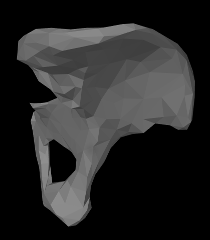
\includegraphics[]{images/hipBodyGray}&
   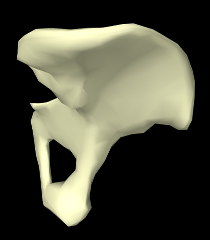
\includegraphics[]{images/hipBodySmooth}&
   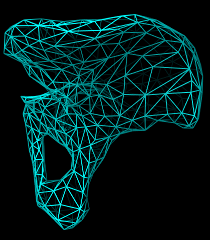
\includegraphics[]{images/hipBodyEdges}\\
 \else
   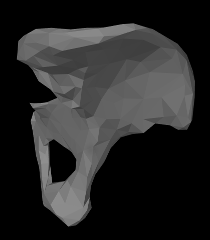
\includegraphics[width=2in]{images/hipBodyGray}&
   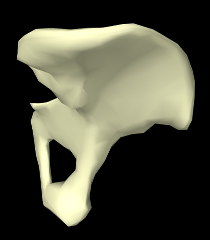
\includegraphics[width=2in]{images/hipBodySmooth}&
   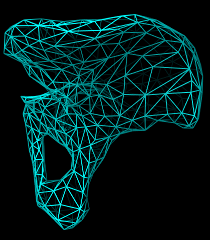
\includegraphics[width=2in]{images/hipBodyEdges}\\
 \fi
\end{tabular}
\end{center}
\caption{Different rendering settings for a rigid body hip mesh
showing the default (left), smooth rendering with a lighter color
(center), and wireframe (right).}
\label{HipRendering:fig}
\end{figure}

Properties can also be set in code, usually during the {\tt build()}
method. Typically this is done using a static method of the
\javaclass[maspack.render]{RenderProps} class that has the form
%
\begin{lstlisting}[]
  RenderProps.setXXX (comp, value)
\end{lstlisting}
%
where {\tt XXX} is the property name, {\tt comp} is the component for
which the property should be set, and {\tt value} is the desired
value. Some examples are shown in Figure \ref{HipRendering:fig} for a
rigid body hip representation with a fairly coarse mesh.  The
left image shows the default rendering, using a gray color and flat
shading. The center image shows a lighter color and smooth shading,
which could be set by the following code fragment:
%
\begin{lstlisting}[]
import maspack.render.*;
import maspack.render.Renderer.*;
  ...

  RigidBody hipBody;
  ...

  RenderProps.setFaceColor (hipBody, new Color (255, 255, 204));
  RenderProps.setShading (hipBody, Shading.SMOOTH);
\end{lstlisting}
%
Finally, the right image shows the body rendered as a wire
frame, which can by done by setting {\sf faceStyle} to {\tt NONE}
and {\sf drawEdges} to {\tt true}:
\begin{lstlisting}[]
  RenderProps.setFaceStyle (hip, FaceStyle.NONE);
  RenderProps.setDrawEdges (hip, true);
  RenderProps.setEdgeWidth (hip, 2);
  RenderProps.setEdgeColor (hip, Color.CYAN);
\end{lstlisting}
%

Render properties can also be set in higher level model components,
from which their values will be inherited by lower level components
that have not explicitly set their own values. For example, setting
the {\sf faceColor} render property in the {\tt MechModel} will
automatically set the face color for all subcomponents which have not
explicitly set {\sf faceColor}. More details on render properties are
given in Section \ref{RenderProperties:sec}.

\begin{figure}[h]
\begin{center}
\begin{tabular}{cc}
 \iflatexml
   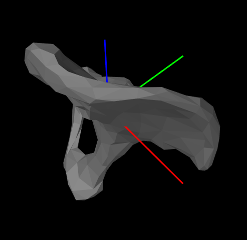
\includegraphics[]{images/hipBodyLineAxes}&
   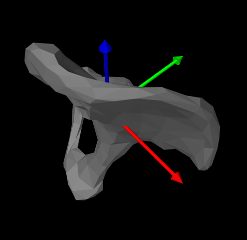
\includegraphics[]{images/hipBodyArrowAxes}\\
 \else
   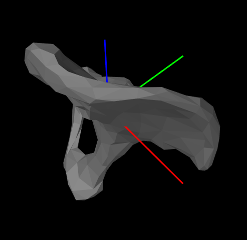
\includegraphics[width=2.5in]{images/hipBodyLineAxes}&
   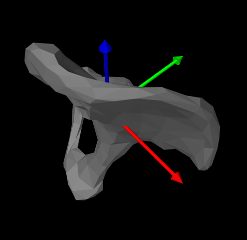
\includegraphics[width=2.5in]{images/hipBodyArrowAxes}\\
 \fi
\end{tabular}
\end{center}
\caption{Rigid body axes rendered with {\sf axisDrawStyle}
set to {\tt LINE} (left) and {\tt ARROW} (right).}
\label{AxisRendering:fig}
\end{figure}

In addition to mesh rendering, it is often useful to draw a rigid
body's coordinate frame, which can be done using its {\sf axisLength}
and {\sf axisDrawStyle} properties. Setting {\sf axisLength} to a
positive value will cause the body's three coordinate axes to be
drawn, with the indicated length, with the $x$, $y$ and $z$ axes
colored red, green, and blue, respectively. The {\tt axisDrawStyle}
property controls how the axes are rendered (Figure
\ref{AxisRendering:fig}). It has the type
\javaclass[maspack.render]{Renderer\$AxisDrawStyle}, and can
be set to the following values:
%
\begin{description}

\item[OFF]\mbox{}

Axes are not rendered.

\item[LINE]\mbox{}

Axes are rendered as simple red-green-blue lines,
with a width given by the joint's {\sf lineWidth} rendering property.

\item[ARROW]\mbox{}

Axes are rendered as solid red-green-blue arrows.

\end{description}
%

As with the rendering proprieties, the {\sf axisLength} and {\sf
axisDrawStyle} properties can be managed either interactively in the
GUI (by selecting the body, right clicking and choosing {\sf Edit
properties ...}), or in code, using the following methods:
% method table
\begin{lstlisting}[]
  double getAxisLength()
  void setAxisLength (double len)

  AxisDrawStyle getAxisDrawStyle()
  void setAxisDrawStyle (AxisDrawStyle style)
\end{lstlisting}
%

\subsection{Multiple meshes}
\label{rigidBodyMultipleMeshes:sec}

A {\tt RigidBody} may contain multiple meshes, which can be useful for
various reasons:

\begin{itemize}

\item It may be desirable to use different meshes for collision
detection, inertia computation, and visual presentation;

\item Different render properties can be set for different mesh
components, allowing the body to be rendered in a more versatile way;

\item Different mesh components can be selected individually.

\end{itemize}

Each rigid body mesh is encapsulated inside a
\javaclass[\mech]{RigidMeshComp} component, which is in turn stored in
a subcomponent list called {\tt meshes}. Meshes do not need to be
instances of \javaclass[maspack.geometry]{PolygonalMesh}; instead,
they can be any instance of \javaclass[maspack.geometry]{MeshBase},
including \javaclass[maspack.geometry]{PointMesh} and
\javaclass[maspack.geometry]{PolylineMesh}.

\begin{sideblock}
The default surface mesh, returned by {\tt getSurfaceMesh()}, is also
stored inside a {\tt RigidMeshComp} in the {\tt meshes} list. By
default, the surface mesh is the first mesh in the list, but is
otherwise defined to be the first mesh in {\tt meshes} which is also
an instance of {\tt PolygonalMesh}. The {\tt RigidMeshComp} containing
the surface mesh can be obtained using the method {\tt
getSurfaceMeshComp()}.
\end{sideblock}

A {\tt RigidMeshComp} contains a number of properties that control how
the mesh is displayed and interacts with its rigid body:

\begin{description}

\item[renderProps]\mbox{}

Render properties controlling how the mesh is
rendered (see Section \ref{RenderProperties:sec}).

\item[hasMass]\mbox{} 

A boolean, which if {\tt true} means that the mesh
will contribute to the body's inertia when the {\sf inertiaMethod}
is either {\tt MASS} or {\tt DENSITY}. The default value is {\tt true}.

\item[massDistribution]\mbox{} 

An enumerated type defined by
\javaclass[maspack.geometry]{MassDistribution} which specifies how the
mesh's inertia contribution is determined for a given mass.  {\tt
VOLUME}, {\tt AREA}, {\tt LENGTH}, and {\tt POINT} indicate,
respectively, that the mass is distributed evenly over the mesh's
volume, area (faces), length (edges), or points. The default value is
determined by the mesh type: {\tt VOLUME} for a closed {\tt
PolygonalMesh}, {\tt AREA} for an open {\tt PolygonalMesh}, {\tt
LENGTH} for a {\tt PolylineMesh}, and {\tt POINT} for a {\tt
PointMesh}. Applications can specify an alternate value providing the
mesh has the features to support it. Specifying {\tt DEFAULT} will
restore the default value.

\item[isCollidable]\mbox{} 

A boolean, which if {\tt true}, and if the mesh is a
{\tt PolygonalMesh}, means that the mesh will take part in collision
and wrapping interactions (Chapter \ref{ContactAndCollision:sec} and
Section \ref{GeneralSurfaceWrapping:sec}). The default value is {\tt true},
and the get/set accessors have the names {\tt isCollidable()} and
{\tt setIsCollidable()}.

\item[volume]\mbox{} 

A double whose value is the volume of the mesh.  If the
mesh is a {\tt PolygonalMesh}, this is the value returned by its
\javamethod[maspack.geometry.PolygonalMesh]{computeVolume()} method.
Otherwise, the volume is 0, unless
\javamethodAlt{\mech.RigidMeshComp.setVolume(double)}{setVolume(vol)} is
used to explicitly set a non-zero volume value.

\item[mass]\mbox{} 

A double whose default value is the product of the {\sf
density} and {\sf volume} properties. Otherwise,
if {\sf mass} has been explicitly set using
\javamethodAlt{\mech.RigidMeshComp.setMass(double)}{setMass(mass)},
the value is the explicit mass.

\item[density]\mbox{}

A double whose default value is the rigid body's
density.  Otherwise, if {\sf density} has been explicitly set using
\javamethodAlt{\mech.RigidMeshComp.setDensity(double)}{setDensity(density)},
the value is the explicit density, or if {\sf mass} has been explicitly
set using
\javamethodAlt{\mech.RigidMeshComp.setMass(double)}{setMass(mass)}, the
value is the explicit {\sf mass} divided by {\sf volume}.

\end{description}

Note that by default, the {\sf density} of a {\tt RigidMeshComp} is
simply the {\sf density} setting for the rigid body, and the {\sf
mass} is this times the {\sf volume}. However, it is possible to set
either an explicit mass or a density value that will override
this. (Also, explicitly setting a mass will unset any explicit
density, and explicitly setting the density will unset any explicit
mass.)

When the {\sf inertiaMethod} of the rigid body is either {\tt MASS} or
{\tt DENSITY}, then its inertia is computed from the sum of all the
inertias $\M_k$ of the component meshes $k$ for which {\sf hasMass} is
{\tt true}. Each $\M_k$ is computed by the mesh's
\javamethodAlt{maspack.geometry.MeshBase.createInertia(double,)}%
{createInertia(mass,massDistribution)} method,
using the {\sf mass} and {\sf massDistribution} properties of
its {\tt RigidMeshComp}.

\begin{sideblock}
When forming the body inertia from the inertia components of
individual meshes, no attempt is made to account for mesh overlap.  If
this is important, the meshes themselves should be modified in advance
so that they do not overlap, perhaps by using the CSG primitives
described in Section \ref{CSG:sec}.
\end{sideblock}

Instances of {\tt RigidMeshComp} can be created directly, using
constructions such as
%
\begin{lstlisting}[]
  PolygonalMesh mesh;

  ... initialize mesh ...

  RigidMeshComp mcomp = new RigidMeshComp (mesh);
\end{lstlisting}
%
or
%
\begin{lstlisting}[]
  RigidMeshComp mcomp = new RigidMeshComp ("meshName");
  mcomp.setMesh (mesh);
\end{lstlisting}
%
after which they can be added or removed from the {\tt meshes} list
using the methods
% method table
\begin{lstlisting}[]
  void addMeshComp (RigidMeshComp mcomp)
  void addMeshComp (RigidMeshComp mcomp, int idx)
  int numMeshComps()
  boolean removeMeshComp (RigidMeshComp mcomp)
  boolean removeMeshComp (String name)
  void clearMeshComps()
\end{lstlisting}
%
It is also possible to add meshes directly to the {\tt meshes} list,
using the methods
% method table
\begin{lstlisting}[]
  RigidMeshComp addMesh (MeshBase mesh)
  RigidMeshComp addMesh (MeshBase mesh, boolean hasMass, boolean collidable)
\end{lstlisting}
%
each of which creates a {\tt RigidMeshComp}, adds it to the mesh list,
and returns it.  The second method also specifies the values of the
{\sf hasMass} and {\sf collidable} properties (both of which are {\tt
true} by default).

\iflatexml
\subsection{Example: a composite rigid body}
\fi

\begin{figure}[ht]
\begin{center}
\iflatexml
 \includegraphics[]{images/RigidCompositeBody}
\else
 \includegraphics[width=3.75in]{images/RigidCompositeBody}
\fi
\end{center}
\caption{{\tt RigidCompositeBody} loaded into ArtiSynth and run for 0.75 seconds.
The ball on the right falls less because it has a lower
density than the rest of the body.}
\label{RigidCompositeBody:fig}
\end{figure}

\iflatexml
\else
\subsection{Example: a composite rigid body}
\fi

An example of constructing a rigid body from multiple meshes is
defined in
%
\begin{verbatim}
  artisynth.demos.tutorial.RigidCompositeBody
\end{verbatim}
%
This uses three meshes to construct a rigid
body whose shape resembles a dumbbell. The code, with the include
files omitted, is listed below:
\lstset{numbers=left}
\iflatexml
%% Hack: latexml lstinputlisting doesn't handle firstline correctly
\lstset{firstnumber={-14}}
\lstinputlisting[firstline=1]{../../src/artisynth/demos/tutorial/RigidCompositeBody.java}
\lstset{firstnumber={1}}
\else
\lstinputlisting[firstline=16]{../../src/artisynth/demos/tutorial/RigidCompositeBody.java}
\fi
\lstset{numbers=none}

As in the previous examples, the {\tt build()} method starts by
creating a {\tt MechModel} (lines 6-7). Three different meshes
(two balls and an axis) are then constructed at lines 10-15,
using {\tt MeshFactory} methods (Section \ref{Meshes:sec})
and transforming each result to an appropriate position/orientation with
respect to the body's coordinate frame.

The body itself is constructed at lines 18-24. Its default density is
set to 10, and its frame damping (Section \ref{RigidBodyDamping:sec})
is also set to 10 (the previous rigid body example in Section 
\ref{RigidBodySpringExample:sec} relied on spring damping to dissipate energy).
The meshes are added using
\javamethod*[\mech.RigidBody]{addMesh()},
which allocates and returns a 
\javaclass[\mech]{RigidMeshComp}. For the ball meshes,
these are saved in {\tt bcomp1} and {\tt bcomp2} and used later to
adjust density and/or render properties.

Lines 27-34 create a simple linear spring, connected to a fixed point
{\tt p0} and a marker {\tt mkr}. The marker is created and attached to
the body by the {\tt MechModel} method
\javamethod*[\mech.MechModel]{addFrameMarkerWorld()}, which places the
marker at a known position in world coordinates.  The spring is
created using an \javaclass[\mech]{AxialSpring} constructor that
accepts a name, along with stiffness, damping, and rest length
parameters to specify a
\javaclass[artisynth.core.materials]{LinearAxialMaterial}.

At line 37, {\tt bcomp1} is used to set the density of {\tt ball1} to
8. Since this is less than the default body density, the inertia
component of {\tt ball1} will be lighter than that of {\tt ball2}.
Finally, render properties are set at lines 41-45. This includes
setting the default face colors for the body and for each ball.

To run this example in ArtiSynth, select {\sf All demos > tutorial >
RigidCompositeBody} from the {\sf Models} menu. The model should load
and initially appear as in Figure \ref{RigidCompositeBody:fig}.
Running the model (Section \ref{LoadingAndRunning:sec}) will cause the
rigid body to fall and swing about under gravity, with the right ball
({\tt ball1}) not falling as far because it has less density.

\section{Mesh components}
\label{MeshComponents:sec}

ArtiSynth models frequently incorporate 3D mesh geometry, as defined
by the geometry classes \javaclass[maspack.geometry]{PolygonalMesh},
\javaclass[maspack.geometry]{PolylineMesh}, and
\javaclass[maspack.geometry]{PointMesh} described in Section
\ref{Meshes:sec}. Within a model, these basic classes are typically
enclosed within container components that are subclasses of
\javaclass[artisynth.core.mechmodels]{MeshComponent}. Commonly
used instances of these include

\begin{description}

\item[\protect{\javaclass[\mech]{RigidMeshComp}}]\mbox{}

Introduced in Section \ref{rigidBodyMultipleMeshes:sec}, these contain
the mesh geometry for rigid bodies, and are stored in a rigid body
subcomponent list named {\tt meshes}. Their mesh vertex positions
are fixed with respect to their body's coordinate frame.

\item[\protect{\javaclass[\fem]{FemMeshComp}}]\mbox{}

Contain mesh geometry associated with finite element models (Chapter
\ref{FEMModels:sec}), including surfaces meshes and embedded mesh
geometry, and are stored in a subcomponent list of the FEM model
named {\tt meshes}. Their mesh vertex positions change as the FEM model
deforms.

\item[\protect{\javaclass[\fem]{SkinMeshBody}}]\mbox{}

Described in detail in Chapter \ref{skinning:sec}, these describe
``skin'' geometry that encloses both rigid bodies and/or FEM models.
Their mesh vertex positions change as the underlying bodies move and
deform. Skinning meshes may be placed anywhere, but are typically
stored in the {\tt meshBodies} component list of a {\tt MechModel}.

\item[\protect{\javaclass[\mech]{FixedMeshBody}}]\mbox{}

Described further below, these store arbitrary mesh geometry
(polygonal, polyline, and point) and provide (like rigid bodies) a
rigid coordinate frame that allows the mesh to be positioned and
oriented arbitrarily. As their name suggests, their mesh vertex
positions are fixed with respect to this coordinate frame. Fixed body
meshes may be placed anywhere, but are typically stored in the {\tt
meshBodies} component list of a {\tt MechModel}.

\end{description}

\subsection{Fixed mesh bodies}
\label{FixedMeshBodies:sec}

As mentioned above, \javaclass[\mech]{FixedMeshBody} can be used for
placing arbitrary mesh geometry within an ArtiSynth model.  These mesh
bodies are non-dynamic: they do not interact or collide with other
model components, and they function primarily as 3D graphical
objects. They can be created from primary mesh components using
constructors such as:
%
\begin{methodtable}{0.5}{0.5}
\midline
%
\methodentry
{\mech .FixedMeshBody.FixedMeshBody(MeshBase)}%
{FixedMeshBody (MeshBase mesh)}%
{Create an unnamed body containing a specified mesh.}%
%
\methodentry
{\mech .FixedMeshBody.FixedMeshBody(String,MeshBase)}%
{FixedMeshBody (String name, MeshBase mesh)}%
{Create a named body containing a specified mesh.}%
%
\midline
\end{methodtable}
%
It should be noted that the primary meshes are not copied and are
instead stored by reference, and so any subsequent changes to them
will be reflected in the mesh body. As with rigid bodies, fixed mesh
bodies contain a coordinate frame, or {\it pose}, that describes the
position and orientation of the body with respect to world
coordinates. Methods to control the pose include:
%
\begin{methodtable}{0.5}{0.5}
\midline
%
\methodentry
{\mech .FixedMeshBody.getPose()}%
{RigidTransform3d getPose()}%
{Returns the pose of the body (with respect to world).}%
%
\methodentry
{\mech .FixedMeshBody.setPose()}%
{void setPose (RigidTransform3d XFrameToWorld)}%
{Sets the pose of the body.}%
\methodspace{0.5em}
%
\methodentry
{\mech .FixedMeshBody.getPosition()}%
{Point3d getPosition()}%
{Returns the body position (pose translation component).}%
%
\methodentry
{\mech .FixedMeshBody.setPosition()}%
{void setPosition (Point3d pos)}%
{Sets the body position.}%
\methodspace{0.5em}
%
\methodentry
{\mech .FixedMeshBody.getOrientation()}%
{AxisAngle getOrientation()}%
{Returns the body orientation (pose rotation component).}%
%
\methodentry
{\mech .FixedMeshBody.setOrientation()}%
{void setOrientation (AxisAngle axisAng)}%
{Sets the body orientation.}%
%
\midline
\end{methodtable}
%
Once created, a canonical place for storing mesh bodies is the {\tt
MechModel} component list {\tt meshBodies}. Methods for
maintaining this list include:
%
\begin{methodtable}{0.5}{0.5}
\midline
%
\methodentry{\mech .MechModel.meshBodies()}%
{ComponentListView<MeshComponent> meshBodies()}%
{Returns the {\tt meshBodies} list.}%
%
\methodentry{\mech .MechModel.addMeshBody()}%
{void addMeshBody (MeshComponent mcomp)}%
{Adds {\tt mcomp} to {\tt meshBodies}.}%
%
\methodentry{\mech .MechModel.removeMeshBody()}%
{boolean removeMeshBody (MeshComponent mcomp)}%
{Removes {\tt mcomp} from {\tt meshBodies}.}%
%
\methodentry{\mech .MechModel.clearMeshBodies()}%
{void clearMeshBodies()}%
{Clears the {\tt meshBodies} list.}%
%
\midline
\end{methodtable}
%
Meshes used for instantiating fixed mesh bodies are typically read
from files (Section \ref{MeshFileIO:sec}), but can also be created
using factory methods (Section \ref{MeshCreation:sec}).  As an
example, the following code fragment creates a torus mesh using a
factory method, set its pose, and then adds it to a {\tt MechModel}:
%
\begin{lstlisting}[]
   MechModel mech;
   ...
   PolygonalMesh mesh = MeshFactory.createTorus (
      /*rmajor=*/1.0, /*rminor=*/0.2, /*nmajor=*/32, /*nminor=*/10);
   FixedMeshBody mbody = new FixedMeshBody ("torus", mesh);
   mbody.setPose (
      new RigidTransform3d (/*xyz=*/0,0,0, /*rpy=*/0,0,Math.toRadians(90)));
   mech.addMeshBody (mbody);
\end{lstlisting}
%

Rendering of mesh bodies is controlled using the same properties
described in Section \ref{rigidBodyRendering:sec} for rigid bodies,
including the {\sf renderProps} subproperties {\sf faceColor}, {\sf
shading}, {\sf alpha}, {\sf faceStyle}, and {\sf drawEdges}, and the
properties {\sf axisLength} and {\sf axisDrawStyle} for displaying a
body's coordinate frame.

\subsection{Example: adding mesh bodies to MechModel}
\label{FixedMeshesExample:sec}

\begin{figure}[h]
\begin{center}
\iflatexml
 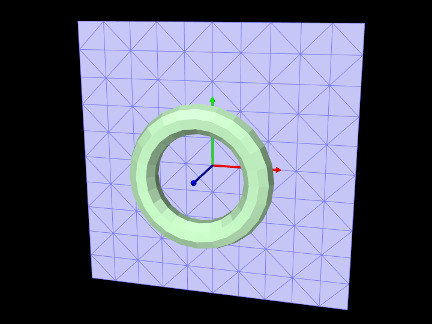
\includegraphics[]{images/FixedMeshes}
\else
 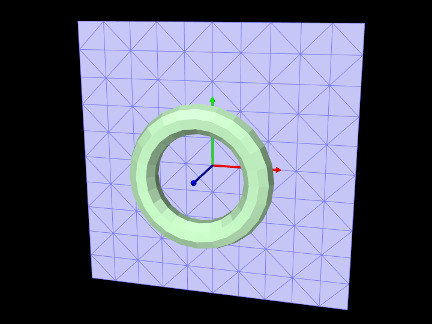
\includegraphics[width=3.75in]{images/FixedMeshes}
\fi
\end{center}
\caption{FixedMeshes model loaded into ArtiSynth.}
\label{FixedMeshes:fig}
\end{figure}

An simple application that creates a pair of fixed meshes and adds
them to a {\tt MechModel} is defined in
%
\begin{verbatim}
  artisynth.demos.tutorial.FixedMeshes
\end{verbatim}
%
The {\tt build()} method for this is shown below:
\lstset{numbers=left}
\iflatexml
%% Hack: latexml lstinputlisting doesn't handle firstline correctly
\lstset{firstnumber={-18}}
\lstinputlisting[firstline=1,lastline=42]{../../src/artisynth/demos/tutorial/FixedMeshes.java}
\lstset{firstnumber={1}}
\else
\lstinputlisting[firstline=20,lastline=61]{../../src/artisynth/demos/tutorial/FixedMeshes.java}
\fi
\lstset{numbers=none}
%
After creating a {\tt MechModel} (lines 3-4), a torus shaped mesh is
imported from the file {\tt data/torus\_9\_24.obj} (lines 8-16). As
described in Section \ref{PathFinder:sec}, the {\tt RootModel} method
{\tt getSourceRelativePath()} is used to locate this file relative to
the model's source folder. The file path is used in the {\tt
PolygonalMesh} constructor, which is enclosed within a {\tt try/catch}
block to handle possible I/O exceptions. Once imported, the mesh is
used to instantiate a {\tt FixedMeshBody} named {\tt "torus"} which is
added to the {\tt MechModel} (lines 18-19).

Another mesh, representing a square, is created with a factory method
and used to instantiate a mesh body named {\tt "square"} (lines
22-26). The factory method specifies both the size and triangle
density of the mesh in the $x$-$y$ plane. Once created, the square's
pose is set to a 90 degree rotation about the $x$ axis and a
translation of 0.5 along $y$ (lines 28-29).

Rendering properties are set at lines 33-41. The torus is made pale
green by setting it face color; the coordinate frame for the square is
made visible as solid arrows using the {\tt axisLength} and {\tt
axisDrawStyle} properties; and the square is made blue gray, with its
edges made visible and drawn using a darker color, and its face style
set to {\tt FRONT\_AND\_BACK} so that it's visible from either side.

To run this example in ArtiSynth, select {\sf All demos > tutorial >
FixedMeshes} from the {\sf Models} menu. The model should load and
initially appear as in Figure \ref{FixedMeshes:fig}.

\section{Joints and connectors}
\label{JointsAndConnectors:sec}

In a typical mechanical model, many of the rigid bodies are
interconnected, either using spring-type components that exert binding
forces on the bodies, or through joints and connectors that enforce
the connection using hard constraints. This section describes the
latter. While the discussion focuses on rigid bodies, joints and
connectors can be used more generally with any body that implements
the \javaclass[artisynth.core.mechmodels]{ConnectableBody}
interface. In particular, this allows joints to also interconnect
finite element models, as described in Section \ref{FEMJoints:sec}.

\subsection{Joints and coordinate frames}
\label{JointsAndFrames:sec}

Consider two rigid bodies A and B. The pose of body B with respect to
body A can be described by the 6 DOF rigid transform $\T_{BA}$.  If A
and B are unconnected, $\T_{BA}$ may assume any possible value and has
a full six degrees of freedom. A {\it joint} between A and B
constrains the set of poses that are possible between the two bodies
and reduces the degrees of freedom available to $\T_{BA}$.  For ease
of use, the constraining action of a joint is described with respect
to a pair of local coordinate frames C and D that are connected to
frames A and B, respectively, by auxiliary transformations.  This
allows joints to be placed at locations that do not correspond
directly to frames A or B.

\begin{figure}[ht]
\begin{center}
 \iflatexml
   \includegraphics[width=2in]{images/jointExample}
 \else
   \includegraphics[width=2in]{images/jointExample}
 \fi
\end{center}
\caption{Coordinate frames D and C for a hinge joint.}
\label{jointExample:fig}
\end{figure}

The joint frames C and D move with respect to each other as the joint
moves. The allowed joint motions therefore correspond to the allowed
values of the {\it joint transform} $\T_{CD}$.  Although both frames
typically move with their attached bodies, D is considered the {\it
base} frame and C the {\it motion} frame (this is because when a joint
is used to connect a single body to ground, body B is set to {\tt
null} and the world frame takes its place).  As an example of a
joint's constraining effect, consider a hinge joint (Figure
\ref{jointExample:fig}), which allows C to move with respect to D {\it only} by
rotating about the $z$ axis while the origins of C and D remain
coincident. Other motions are prohibited. If we let $\theta$ describe
the counter-clockwise rotation angle of C about the $z$ axis, then
$\T_{CD}$ should always have the form
%
\begin{equation}
\T_{CD} = \matl
\cos(\theta) & -\sin(\theta) & 0 & 0 \\
\sin(\theta) &  \cos(\theta) & 0 & 0 \\
0 & 0 & 1 & 0 \\
0 & 0 & 0 & 1 
\matr.
\end{equation}
%

\begin{figure}[ht]
\begin{center}
 \iflatexml
   \includegraphics[width=3.74in]{images/jointBodyFrames}
 \else
   \includegraphics[width=3.74in]{images/jointBodyFrames}
 \fi
\end{center}
\caption{Transforms connecting joint coordinate frames C and D with
rigid bodies A and B.}
\label{jointBodyFrames:fig}
\end{figure}

When a joint is attached to bodies A and B, frame C is fixed to body A
and frame D is fixed to body B. Except in special cases, the joint
frames C and D are not coincident with the body frames A
and B.  Instead, they are located relative to A and B by the
transforms $\T_{CA}$ and $\T_{DB}$, respectively
(Figure \ref{jointBodyFrames:fig}). Since $\T_{CA}$ and $\T_{DB}$ are
both fixed, the joint constraints on $\T_{CD}$ constrain the relative
poses of A and B, with $\T_{AB}$ determined from
%
\begin{equation}
\T_{AB} = \T_{DB} \, \T_{CD} \, \T_{CA}^{-1}.
\label{jointPose:eqn}
\end{equation}
%
(See Section \ref{RigidTransforms:sec} for a discussion of determining
transforms between related coordinate frames).

\subsection{Joint coordinates, constraints, and errors}
\label{JointCoordinates:sec}

Each different joint and connector type restricts the motion between
two bodies to $M$ degrees of freedom, for some $M < 6$.  Sometimes,
the joint also defines a set of $M$ coordinates that parameterize
these $M$ DOFs. For example, the hinge joint described above is
parameterized by $\theta$. Other examples are given in
Section \ref{JointTypes:sec}: a 2 DOF cylindrical has coordinates $z$
and $\theta$, a 3 DOF gimbal joint is parameterized by the
roll-pitch-yaw angles $\theta$, $\phi$, and $\psi$, etc.  When
$\T_{CD} = \I$ (where $\I$ is the identity transform), the coordinates
are usually all equal to zero, and the joint is said to be in the {\it
zero state}.

As explained in Section \ref{PhysicsSimulation:sec}, ArtiSynth uses a
full coordinate formulation for dynamic simulation. That means that
instead of using joint coordinates to describe system state, it uses
the combined full coordinates $\q$ of all dynamic components. For
example, a model consisting of a single rigid body connected to ground
by a hinge joint will have 6 DOF (corresponding to the 6 DOF of the
body), rather than the 1 DOF implied by the hinge joint.  The DOF
restrictions imposed by the joints are then enforced by a set of
linearized constraint relationships
%
\begin{equation}
\G(\q) \u = \g, \qquad \N(\q) \u \ge \n
\label{constraints2:eqn}
\end{equation}
%
that restrict the body velocities $\u$ computed at each simulation
step, usually by solving an MLCP like (\ref{KKTvelocity:eqn}). As
explained in Section \ref{PhysicsSimulation:sec}, the right side
vectors $\g$ and $\n$ in (\ref{constraints2:eqn}) contain time
derivative terms, which for simplicity much of the following
presentation will assume to be 0.

Each joint contributes its own set of constraint equations to
(\ref{constraints2:eqn}). Typically these take the form of {\it
bilateral}, or equality, constraints
%
\begin{equation}
\G_\text{J}(\q) \u = 0
\label{bilateralG:eqn}
\end{equation}
%
which are added to the system's global bilateral constraint matrix
$\G$. $\G_\text{J}$ contains $6 - M$ rows providing $6 - M$ individual
constraints $\G_k$.
During simulation, these give rise to $6 - M$ constraint
forces (corresponding to $\Blam$ in (\ref{impulsesToForces:eqn}))
which enforce the constraints.

In some cases, the joint also maintains {\it unilateral}, or inequality
constraints, to keep $\T_{CD}$ out of inadmissible regions. These take
the form
%
\begin{equation}
\N_\text{J}(\q) \u \ge 0
\label{unilateralN:eqn}
\end{equation}
%
and are added to the system's global unilateral constraint matrix
$\N$.  They give rise to constraint forces corresponding to $\Bthe$ in
(\ref{impulsesToForces:eqn}). A common use of unilateral constraints
is to enforce range limits of the joint coordinates (Section
\ref{coordinateLimitsAndLocking:sec}), such as
%
\begin{equation}
\theta_{\text{min}} \le \theta \le \theta_{\text{max}}.
\end{equation}
%
A specific unilateral constraint is added to $\N_\text{J}$ only when
$\T_{CD}$ is on or within the boundary of the inadmissible region
associated with that constraint. The constraint is then said to be
{\it engaged}. The combined number of bilateral and engaged unilateral
constraints for a particular joint should not exceed 6; otherwise, the
joint would be overconstrained.

Joint coordinates, when supported for a particular joint, can be both
read and set. Setting a coordinate causes the joint transform
$\T_{CD}$ to change. To accommodate this, the system adjusts the poses
of one or both bodies connected to the joint, along with adjacent
bodies connected to them, with preference given to bodies that are not
attached to ``ground''.  However, if this is done during simulation,
and particularly if one or both of the bodies connected to the joint
are moving dynamically, the results will be unpredictable and will
likely conflict with the simulation.

Joint coordinates are also often exported as properties. For example,
the
\javaclass[artisynth.core.mechmodels]{HingeJoint}
class (Section \ref{JointTypes:sec}) exports its $\theta$ coordinate
as the property {\sf theta}, which can be accessed in the GUI, or via
the accessor methods
% method table
\begin{lstlisting}[]
  double getTheta()          // get theta in degrees

  void setTheta (double deg) // set theta in degrees
\end{lstlisting}
%

Since joint constraints are generally nonlinear, their linearized
enforcement at the velocity level by (\ref{constraints2:eqn}) will
usually produce small errors as the simulation proceeds.  These errors
are reduced using a position correction step described in
Section \ref{JointConstraints:sec} and \cite{lloyd2012artisynth}.
Errors can also be caused by joint compliance
(Section \ref{JointCompliance:sec}).  Both effects mean that the joint
transform $\T_{CD}$ may deviate from the allowed values dictated by
the joint type. In ArtiSynth, this is accounted for by introducing an
additional {\it constraint} frame G between D and C
(Figure \ref{jointFrames:fig}).  G is computed to be the nearest frame
to C that lies exactly in the joint constraint space. $\T_{GD}$ is
therefore a valid joint transform, $\T_{GC}$ accommodates the error,
and the whole joint transform is given by the composition
%
\begin{equation}
\T_{CD} = \T_{GD} \; \T_{CG}.
\end{equation}
%
If there is no compliance or joint error, then frames G and C are
identical, $\T_{CG} = \I$, and $\T_{CD} = \T_{GD}$.  Because $\T_{CG}$
describes the joint error, we sometimes refer to it as $\T_{err}
= \T_{CG}$.

\begin{figure}[ht]
\begin{center}
 \iflatexml
   \includegraphics[width=3.5in]{images/jointFrames}
 \else
   \includegraphics[width=3.5in]{images/jointFrames}
 \fi
\end{center}
\caption{2D schematic showing the joint frames D and C, along with
the intermediate frame G that accounts for numeric error
and complaint motion.}
\label{jointFrames:fig}
\end{figure}

\subsection{Creating joints}
\label{CreatingJoints:sec}

Joint and connector components in ArtiSynth are both derived from the
superclass
\javaclass[artisynth.core.mechmodels]{BodyConnector},
with joints being further derived from
\javaclass[artisynth.core.mechmodels]{JointBase},
which provides support for coordinates.  Some of the commonly used
joints and connectors are described in Section
\ref{JointTypes:sec}.

An application creates a joint by constructing it and adding it to a
{\tt MechModel}. Many joints have constructors of the form
%
\begin{lstlisting}[]
  XXXJoint (bodyA, bodyB, TDW)
\end{lstlisting}
%
which specifies the bodies A and B which the joint connects,
along with the transform $\T_{DW}$ giving the pose of the joint base
frame D in world coordinates. The constructor then assumes that the
joint is in the zero state, so that C and D are the same and
$\T_{CD} = \I$ and $\T_{CW} = \T_{DW}$, and then computes
$\T_{CA}$ and $\T_{DB}$ from
%
\begin{align}
\T_{CA} & = \T_{AW}^{-1} \; \T_{CW} \\
\T_{DB} & = \T_{BW}^{-1} \; \T_{DW},
\end{align}
%
where $\T_{AW}$ and $\T_{BW}$ are the current poses of A and B.

After the joint is created, it should be added to the system's {\tt
MechModel} using
\javamethod[artisynth.core.mechmodels.MechModel]{addBodyConnector()}, as
shown in the following code fragment:
%
\begin{lstlisting}[]
   MechModel mech; 
   RigidBody bodyA, bodyB;
   RigidTransform3d TDW;

   ... initialize mech, bodyA, bodyB, and TDW ...
   
   HingeJoint joint = new HingeJoint (bodyA, bodyB, TDW);
   mech.addBodyConnector (joint);
\end{lstlisting}
%
It is also possible to create a joint using its default
constructor and attach it to the bodies
afterward, using the method 
\javamethodAlt{%
artisynth.core.mechmodels.BodyConnector.setBodies(,,)}
{setBodies(bodyA,bodyB,TDW)}, as in the following:
%
\begin{lstlisting}[]
   HingeJoint joint = new HingeJoint ();
   joint.setBodies (bodyA, bodyB, TDW);
   mech.addBodyConnector (joint);
\end{lstlisting}
%
One reason for doing this is that it allows the joint transform
$\T_{CD}$ to be modified (by setting coordinate values) {\it before}
{\tt setBodies()} is called; this is discussed further in
Section \ref{workingWithCoordinates:sec}.

Joints usually offer a number of other constructors that let its world
location and body relationships to be specified in different
ways. These may include:
%
\begin{lstlisting}[]
  XXXJoint (bodyA, TCA, bodyB, TDB)

  XXXJoint (bodyA, bodyB, TCW, TDW)
\end{lstlisting}
%
The first, which is restricted to rigid bodies, allows the application
to explicitly specify transforms $\T_{CA}$ and $\T_{DB}$ connecting
frames C and D to the body frames A and B, and is useful when
$\T_{CA}$ and $\T_{DB}$ are explicitly known, or the initial value of
$\T_{CD}$ is {\it not} the identity. Likewise, the second constructor
allows $\T_{CW}$ and $\T_{DW}$ to be explicitly specified, with
$\T_{CD} \ne \I$ if $\T_{CW} \ne \T_{DW}$.  For instance, suppose
$\T_{CD}$ and $\T_{DW}$ are both known. Then we can use the
relationship
%
\begin{equation}
\T_{CW} = \T_{DW} \, \T_{CD}
\end{equation}
%
to create the joint as in the following code fragment:
%
\begin{lstlisting}[]
   MechModel mech;
   RigidBody bodyA, bodyB;
   RigidTransform3d TDW, TCD;

   ... initialize mech, bodyA, bodyB, TDW, and TCD ...

   // compute TCW:
   RigidTransform3d TCW = new RigidTransform3d();
   TCW.mul (TDW, TCD);
   HingeJoint joint = new HingeJoint (bodyA, bodyB, TCW, TDW);
   mech.addBodyConnector (joint);
\end{lstlisting}
%

As an alternative to specifying $\T_{DW}$ or its equivalents, some
joint types provide constructors that let the application locate
specific joint features. These may be easier to use in some cases. For
instance, \javaclass[artisynth.core.mechmodels]{HingeJoint} provides a
constructor
% method table
\begin{lstlisting}[]
   HingeJoint (bodyA, bodyB, originD, zaxis)
\end{lstlisting}
%
that specifies origin of D and its $z$ axis (which is the rotation
axis), with the remaining orientation of D aligned as closely as
possible with the world.
\javaclass[artisynth.core.mechmodels]{SphericalJoint} provides a
constructor
% method table
\begin{lstlisting}[]
   SphericalJoint (bodyA, bodyB, originD)
\end{lstlisting}
%
that specifies origin of D and aligns its orientation with the world.
Users should consult the source code or API documentation for specific
joints to see what special constructors may be available.

Finally, it is possible to use joints to connect a single body to
ground (by convention, this is the A body). Most joints provide a
constructor of the form
%
\begin{lstlisting}[]
  XXXJoint (bodyA, TDW)
\end{lstlisting}
%
which allows this to be done explicitly. Alternatively, most joint
constructors which supply body B will allow this to be specified as
{\tt null}, so that body A will be connected to ground by default.

\subsection{Working with coordinates}
\label{workingWithCoordinates:sec}

As mentioned in Section \ref{JointCoordinates:sec}, some joints
support coordinates that parameterize the valid motions within the
joint transform $\T_{CD}$. All such joints are subclasses of
\javaclass[artisynth.core.mechmodels]{JointBase},
which provides some generic methods for querying and setting
coordinate values ({\tt JointBase} is in turn a subclass of
\javaclass[artisynth.core.mechmodels]{BodyConnector}).

The number of coordinates is returned by the method {\tt
numCoordinates()}; if this returns 0, then coordinates are not
supported. Each coordinate has an index in the range $0 \ldots M-1$,
where $M$ is the number of coordinates. Coordinate values can be
queried or set using the following methods:
% method table
\begin{lstlisting}[]
  getCoordinate (int idx)               // get coordinate value with index idx
  getCoordinates (VectorNd coords)      // get all coordinates values

  setCoordinate (int idx, double value) // set coordinate value with index idx
  setCoordinates (VectorNd values)      // set all coordinates values
\end{lstlisting}
%

Specific joint types usually also provide names for their joint
coordinates, along with integer constants describing their indices
and methods for accessing their values. For example,
\javaclass[artisynth.core.mechmodels]{CylindricalJoint}
supports two coordinates, $z$ and $\theta$, along with
the following:
%
\begin{lstlisting}[]
  // coordinate indices
  static final int Z_IDX = 0;
  static final int THETA_IDX = 1;

  // set/get z value and range
  double getZ()
  void setZ (double z)

  // set/get theta value and range in degrees
  double getTheta()
  void setTheta (double theta)
\end{lstlisting}
%
The coordinate values are also exported as the properties {\sf z} and
{\sf theta}, allowing them to be set in the GUI. For convenience,
particularly in GUI applications, the properties and methods for
controlling specific angular coordinates generally use degrees instead
of radians.

As discussed in Section \ref{JointCoordinates:sec}, unlike in some
multibody simulation systems (such as OpenSim), joint coordinates are
{\it not} fundamental quantities that describe system state. As such,
then, coordinates can usually only be set in specific circumstances
that avoid simulation conflicts. In general, when joint coordinates
are set, the system adjusts the poses of one or both bodies connected
to this joint, along with adjacent bodies connected to them, with
preference given to bodies that are not attached to ``ground''.
However, if this is done during simulation, and particularly if one or
both of the bodies connected to the joint are moving dynamically, the
results will be unpredictable and will likely conflict with the
simulation.

If a joint has been created with its default constructor and not yet
attached to any bodies, then setting joint values will simply set the
joint transform $\T_{CD}$. This can be useful in situations where one
needs to initialize a joint's $\T_{CD}$ to a non-identity value
corresponding to a particular set of joint coordinates:
%
\begin{lstlisting}[]
  RigidTransform3d TDW; // known location for D frame
  double z, theta; // desired initial coordinate values
  ...
  CylindricalJoint joint = new CylindricalJoint();
  joint.setZ (z);
  joint.setTheta (thetaDeg);
  joint.setBodies (bodyA, bodyB, TDW);
\end{lstlisting}
%
This can also be done in vector form:
%
\begin{lstlisting}[]
  RigidTransform3d TDW; // known location for D frame
  VectorNd coordValues; // desired initial coordinate values
  ...
  CylindricalJoint joint = new CylindricalJoint();
  joint.setCoordinates (coordValues);
  joint.setBodies (bodyA, bodyB, TDW);
\end{lstlisting}
%
In either of these cases, {\tt setBodies()} will not use $\T_{CD}
= \I$ but instead use the value determined by the initial coordinate
values.

To determine the $\T_{CD}$ corresponding to a particular set of
coordinates, one may use the method
% method table
\begin{lstlisting}[]
  void coordinatesToTCD (RigidTransform3d TCD, VectorNd coords)
\end{lstlisting}
%

In some cases, within a model's {\tt build()} method, one may wish to
set initial coordinates {\it after} a joint has been attached to its
bodies, in order to move those bodies (along with the bodies attached
to them) into an initial configuration without having to explicitly
calculate the poses from the joint coordinates. As mentioned
above, the system will make a decision about which attached bodies are
most ``free'' and adjust their poses accordingly. This is done in the
example of the next section.

\subsection{Coordinate limits and locking}
\label{coordinateLimitsAndLocking:sec}

It is possible to set limits on a joint coordinate's range, and also
to lock a coordinate in place at its current value.

When a joint coordinate hits either an upper or lower range limit, a
unilateral constraint is invoked to prevent it from violating the
limit, and remains engaged until the joint moves away from the
limit. Each range constraint that is engaged reduces the number of
joint DOFs by one.

By default, joint range limits are usually disabled (i.e., they are
set to $(-\inf, \inf)$). They can be queried and set, for a given
joint with index {\tt idx}, using the methods:
% method table
\begin{lstlisting}[]
  DoubleInterval getCoordinateRange (int idx)	
  double getMinCoordinate (int idx)
  double getMaxCoordinate (int idx)
  void setCoordinateRange (idx, DoubleInterval rng)
\end{lstlisting}
%
where range limits for angular coordinates are specified in
radians. For convenience, the following methods are also provided
which use degrees instead of radians for angular coordinates:
% method table
\begin{lstlisting}[]
  DoubleInterval getCoordinateRangeDeg (int idx)
  double getMinCoordinateDeg (int idx)
  double getMaxCoordinateDeg (int idx)
  void setCoordinateRangeDeg (idx, DoubleInterval rng)
\end{lstlisting}
%
Range checking can be disabled by setting the range to
$(-\inf, \inf)$, or by specifying {\tt rng} as {\tt null}, which
implicitly does the same thing.

\begin{sideblock}
Ranges for angular coordinates are not limited to $\pm 180^\circ$ but
can instead be set to larger values; the joint will continue to wrap
until the limit is reached.
\end{sideblock}

Joint coordinates can also be {\it locked}, so that they hold their
current value and don't move. A joint is locked using a bilateral
constraint that prevents motion in either direction and reduces the
joint's DOF count by one.  The following methods are available for
querying or setting a coordinate's locked status:
% method table
\begin{lstlisting}[]
  boolean isLocked (int idx)	
  void setLocked (int idx, boolean locked)
\end{lstlisting}
%

As with coordinate values, specific joint types usually provide
methods for controlling the ranges and locking status of individual
coordinates, with ranges for angular coordinates specified in degrees
instead of radians.  For example,
\javaclass[artisynth.core.mechmodels]{CylindricalJoint}
supplies the methods
% method table
\begin{lstlisting}[]
  // set/get z range
  DoubleInterval getZRange()
  void setZRange (double min, double max)

  // control z locking
  boolean isZLocked()
  void setZLocked (boolean locked)

  // set/get theta range in degrees
  DoubleInterval getThetaRange()
  void setThetaRange (double min, double max)
  void setThetaRange (DoubleInterval rng)

  // control theta locking
  boolean isThetaLocked()
  void setThetaLocked (boolean locked)
\end{lstlisting}
%
The range and locking information is also exported as the properties
{\sf zRange}, {\sf thetaRange}, {\sf zLocked}, and {\sf thetaLocked},
allowing them to be set in the GUI.

\subsection{Example: a simple hinge joint}
\label{RigidBodyJoint:sec}

\begin{figure}[ht]
\begin{center}
\iflatexml
 \includegraphics[]{images/RigidBodyJoint}
\else
 \includegraphics[width=3.75in]{images/RigidBodyJoint}
\fi
\end{center}
\caption{RigidBodyJoint model loaded into ArtiSynth.}
\label{RigidBodyJoint:fig}
\end{figure}

A simple model showing two rigid bodies connected by
a joint is defined in
%
\begin{verbatim}
  artisynth.demos.tutorial.RigidBodyJoint
\end{verbatim}
%

The build method for this model is given below:
\lstset{numbers=left}
\begin{lstlisting}[]
   public void build (String[] args) {

      // create MechModel and add to RootModel
      mech = new MechModel ("mech");
      mech.setGravity (0, 0, -98);
      mech.setFrameDamping (1.0);
      mech.setRotaryDamping (4.0);
      addModel (mech);

      PolygonalMesh mesh;  // bodies will be defined using a mesh

      // create first body and set its pose
      mesh = MeshFactory.createRoundedBox (lenx1, leny1, lenz1, /*nslices=*/8);
      RigidTransform3d TMB = 
         new RigidTransform3d (0, 0, 0, /*axisAng=*/1, 1, 1, 2*Math.PI/3);
      mesh.transform (TMB);
      bodyB = RigidBody.createFromMesh ("bodyB", mesh, /*density=*/0.2, 1.0);
      bodyB.setPose (new RigidTransform3d (0, 0, 1.5*lenx1, 1, 0, 0, Math.PI/2));
      bodyB.setDynamic (false);

      // create second body and set its pose
      mesh = MeshFactory.createRoundedCylinder (
         leny2/2, lenx2, /*nslices=*/16, /*nsegs=*/1, /*flatBottom=*/false);
      mesh.transform (TMB);
      bodyA = RigidBody.createFromMesh ("bodyA", mesh, 0.2, 1.0);
      bodyA.setPose (new RigidTransform3d (
                        (lenx1+lenx2)/2, 0, 1.5*lenx1, 1, 0, 0, Math.PI/2));

      // create the joint      
      RigidTransform3d TDW = 
         new RigidTransform3d (lenx1/2, 0, 1.5*lenx1, 1, 0, 0, Math.PI/2);
      HingeJoint joint = new HingeJoint (bodyA, bodyB, TDW);

      // add components to the mech model
      mech.addRigidBody (bodyB);
      mech.addRigidBody (bodyA);
      mech.addBodyConnector (joint);

      joint.setTheta (35);  // set joint position

      // set render properties for components
      RenderProps.setFaceColor (joint, Color.BLUE);
      joint.setShaftLength (4);
      joint.setShaftRadius (0.2);
   }
\end{lstlisting}
\lstset{numbers=none}

A {\tt MechModel} is created as usual at line 4. However, in this
example, we also set some parameters for it:
\javamethod*[artisynth.core.mechmodels.MechModel]{setGravity()} is
used to set the gravity acceleration vector to $(0, 0, -98)^T$ instead
of the default value of $(0, 0, -9.8)^T$, and the {\tt frameDamping}
and {\tt rotaryDamping} properties (Section
\ref{RigidBodyDamping:sec}) are set to provide appropriate damping.

Each of the two rigid bodies are created from a mesh and a density.
The meshes themselves are created using the factory methods
\javamethod*[maspack.geometry]{MeshFactory.createRoundedBox()} and
\javamethod*[maspack.geometry]{MeshFactory.createRoundedCylinder()}
(lines 13 and 22), and then
\javamethod*[artisynth.core.mechmodels]{RigidBody.createFromMesh()} is
used to turn these into rigid bodies with a density of 0.2 (lines 17
and 25). The pose of the two bodies is set using {\tt
RigidTransform3d} objects created with x, y, z translation and
axis-angle orientation values (lines 18 and 26).

The hinge joint is implemented using
\javaclass[artisynth.core.mechmodels]{HingeJoint}, which is
constructed at line 32 with the joint coordinate frame D being located
in world coordinates by {\tt TDW} 
as described in Section \ref{CreatingJoints:sec}.

Once the joint is created and added to the {\tt MechModel}, the method
\javamethod*[artisynth.core.mechmodels.HingeJoint]{setTheta()} is
used to explicitly set the joint parameter to 35 degrees. The joint
transform $\T_{CD}$ is then set appropriately and {\tt bodyA} is moved
to accommodate this ({\tt bodyA} being chosen since it is the most
free to move).

Finally, joint rendering properties are set starting at line 42. We
render the joint as a cylindrical shaft about the rotation axis, using
its {\sf shaftLength} and {\sf shaftRadius} properties. Joint
rendering is discussed in more detail in
Section \ref{RenderingJoints:sec}).

To run this example in ArtiSynth, select {\sf All demos > tutorial >
RigidBodyJoint} from the {\sf Models} menu. The model should load and
initially appear as in Figure \ref{RigidBodyJoint:fig}.  Running the
model (Section \ref{LoadingAndRunning:sec}) will cause {\tt bodyA} to
fall and swing under gravity.

\subsection{Constraint forces}

During each simulation solve step, the joint velocity constraints
described by (\ref{bilateralG:eqn}) and (\ref{unilateralN:eqn}) are
enforced by bilateral and unilateral constraint forces $\f_g$ and
$\f_n$:
%
\begin{equation}
\f_g = \G_\text{J}^T \Blam_J, \quad \f_n = \N_\text{J}^T \Bthe_J.
\end{equation}
%
Here, $\f_g$ and $\f_n$ are spatial forces (or {\it wrenches}, Section
\ref{SpatialVelocitiesAndForces:sec}) acting in the joint coordinate
frame C, and $\Blam_J$ and $\Bthe_J$ are the Lagrange multipliers
computed as part of the mechanical system solve (see
(\ref{KKTvelocity:eqn}) and (\ref{impulsesToForces:eqn})).  The sizes
of $\Blam_J$ and $\Bthe_J$ equal the number of bilateral and {\it
engaged} unilateral constraints in the joint; these numbers can be
queried for a particular joint using the methods
\javamethod[artisynth.core.mechmodels.BodyConnector]{numBilateralConstraints()}
and
\javamethod[artisynth.core.mechmodels.BodyConnector]{%
numEngagedUnilateralConstraints()}.
(The number of engaged unilateral constraints may be less than the
total number of unilateral constraints; the latter may be queried with
\javamethod[artisynth.core.mechmodels.BodyConnector]{numUnilateralConstraints()},
while the total number of
constraints is returned by
\javamethod[artisynth.core.mechmodels.BodyConnector]{numConstraints()}.

Applications may sometimes need to query the current constraint force
values, typically from within a controller
or monitor (Section \ref{ControllersAndMonitors:sec}).
The Lagrange multipliers themselves may be obtained with
% method table
\begin{lstlisting}[]
  void getBilateralForces (VectorNd lam)

  void getUnilateralForces (VectorNd the)
\end{lstlisting}
%
which load the multipliers into {\tt lam} or {\tt the} and set their
sizes to the number of bilateral or engaged unilateral
constraints. Alternatively, one can retrieve the individual multiplier
for the constraint indexed by {\tt idx} using
% method table
\begin{lstlisting}[]
  double getConstraintForce (int idx);
\end{lstlisting}
%

Typically, it is more useful to find the spatial constraint forces
$\f_g$ and $\f_n$, which can be obtained with respect to frame C:
% method table
\begin{lstlisting}[]
  // place the forces in the wrench f
  void getBilateralForcesInC (Wrench f)
  void getUnilateralForcesInC (Wrench f)

  // convenience methods that allocate the wrench and return it
  Wrench getBilateralForcesInC();
  Wrench getUnilateralForcesInC();
\end{lstlisting}
%
If the attached bodies A and B are rigid bodies, it is also possible
to obtain the constraint wrenches experienced by those bodies:
% method table
\begin{lstlisting}[]
  // place the forces in the wrench f
  void getBilateralForcesInA (Wrench f)
  void getUnilateralForcesInA (Wrench f)
  void getBilateralForcesInB (Wrench f)
  void getUnilateralForcesInB (Wrench f)

  // convenience methods that allocate the wrench and return it
  Wrench getBilateralForcesInA();
  Wrench getUnilateralForcesInA();
  Wrench getBilateralForcesInB();
  Wrench getUnilateralForcesInB();
\end{lstlisting}
%
Constraint wrenches obtained for bodies A or B are given in world
coordinates, which is consistent with the forces reported by rigid
bodies via their {\tt getForce()} method. To orient the forces into
body coordinates, one may use the inverse of the rotation matrix $\R$
of the body's pose. For example:
%
\begin{lstlisting}[]
   RigidBody bodyA;

   // ... body A initialized, etc. ...

   Wrench force = joint.getBilateralForceInA();
   force.inverseTransform (bodyA.getPose().R);
\end{lstlisting}
%

\subsection{Compliance and regularization}
\label{JointCompliance:sec}

By default, the constraints used to implement joints and couplings are
treated as {\it hard}, so that the system tries to respect the
constraint conditions (\ref{constraints2:eqn}) as exactly as possible
as the simulation proceeds.  Sometimes, however, it is desirable to
introduce some ``softness'' into the constraints, whereby constraint
forces are determined as a linear function of their distance from the
constraint. Adding compliance also allows an application to {\it
regularize} a system of joint constraints that would otherwise be
overconstrained, as illustrated in Section \ref{FourBar:sec}.

To describe compliance precisely, consider the bilateral constraint
portion of the MLCP in (\ref{KKTvelocity:eqn}), which solves for the
updated system velocities $\u^{k+1}$ at each time step:
%
\begin{equation}
\matl
\hat\M^{k} & -\G^{T} \\
\G & 0
\matr
\matl
\u^{k+1} \\
\tilde\Blam
\matr
=
\matl
\M \u^{k} - h \hat\f^{k} \\
0
\matr.
\label{KKThard:eqn}
\end{equation}
%
Here $\G$ is the system's bilateral constraint matrix, $\tilde\Blam$
denotes the constraint impulses (from which the constraint forces
$\Blam$ can be determined by $\Blam = \tilde\Blam/h$), and for
simplicity we have assumed that $\G$ is constant and so the $\g$ term
on the lower right side is $0$.

Solving (\ref{KKThard:eqn}) results in constraint forces that satisfy
$\G \u^{k+1} = 0$ precisely, corresponding to hard constraints. To
implement soft constraints, start by defining a function $\Bphi(\q)$
that defines the {\it distances} from each constraint, where $\q$ is the
vector of system positions; these distances are
the local translational and rotational deviations from each
constraint's correct position and are discussed in more detail in
Section \ref{JointConstraints:sec}. Then assume that the constraint
forces are a linear function of these distances:
%
\begin{equation}
\Blam = -\C^{-1} \Bphi(\q),
\label{compliance:eqn}
\end{equation}
%
where $\C$ is a diagonal {\it compliance} matrix that is equivalent to
an inverse stiffness matrix. We also note that $\Bphi$ will be time
varying, and that we can approximate its change between time steps as
%
\begin{equation}
\Bphi^{k+1} \approx \Bphi^k + h \dot\Bphi^{k+1}, \quad \text{with}
\quad \dot\Bphi^{k+1} = \G \u^{k+1}.
\label{BphiApprox:eqn}
\end{equation}
%
Next, assume that in using (\ref{compliance:eqn}) to determine $\Blam$
for a particular time step, we use the {\it average} value of $\Bphi$
over the step, represented by $\bar\Bphi = (\Bphi^{k+1} + \Bphi^k)/2$.
Substituting this and (\ref{BphiApprox:eqn}) into
(\ref{compliance:eqn}), multiplying by $\C$, and rearranging yields:
%
\begin{equation}
\G \u^{k+1} + \frac{2 \C}{h} \Blam = -\frac{2}{h} \Bphi^k.
\end{equation}
%
Then noting that $\tilde\Blam = h \Blam$, we obtain
a revised form of (\ref{KKThard:eqn}),
%
\begin{equation}
\matl
\hat\M^{k} & -\G^{T} \\
\G & 2 \C /h^2 
\matr
\matl
\u^{k+1} \\
\tilde\Blam
\matr
=
\matl
\M \u^{k} - h \hat\f^{k} \\
- 2 \Bphi^k/h
\matr,
\label{KKTsoft:eqn}
\end{equation}
%
in the which the zeros in the matrix and right hand side have been
replaced by compliance terms.
The resulting constraint behavior is different from that of
(\ref{KKThard:eqn}) in two important ways:

\begin{enumerate}

\item The joint now allows 6 DOF, with motion along the constrained directions
limited by restoring spring constants given by the reciprocals of the
diagonal entries of $\C$.

\item If $\C$ has no zero diagonal entries, then the system
(\ref{KKTsoft:eqn}) is {\it regularized} by the $2 \C/h^2$ term in the
lower right matrix block. This means that the matrix is always
non-singular, even if $\G$ is rank deficient, and so compliance offers
a way to handle overconstrained models, as discussed further in
Section \ref{FourBar:sec}.

\end{enumerate}

Unilateral constraints can be regularized using the same approach,
with a distance function defined such that $\Bphi(\q) \le 0$.  

The reason for specifying soft constraints using compliance instead of
stiffness is that by setting $\C = 0$ we can easily handle the case of
{\it infinite} stiffness where the constraints are strictly enforced.
The ArtiSynth compliance implementation uses a slightly more complex
version of (\ref{KKTsoft:eqn}) that accounts for non-constant $\G$ and
also allows for a damping term $-\D \dot\Bphi$, where $\D$ is again a
diagonal matrix.  For more details, see \cite{lacoursiere2007ghosts}
and \cite{servin2006interactive}.

When using compliance, damping is often needed for stability, and, in
the case of unilateral constraints, to prevent ``bouncing''.  A good
choice for damping is usually {\it critical damping}, which is
discussed further below.

Any joint which is a subclass of
\javaclass[artisynth.core.mechmodels]{BodyConnector} allows
individual compliance values $C_i$ and damping values $D_i$ to be set
for each of the joint's $i$ constraints. These values comprise the
diagonal entries in the compliance and damping matrices $\C$ and $\D$,
and can be queried and set using the methods
% method table
\begin{lstlisting}[]
  VectorNd getCompliance()
  void setCompliance (VectorNd compliance)

  VectorNd getDamping()
  void setCompliance (VectorNd damping)
\end{lstlisting}
%
The vectors supplied to the above {\tt set} methods contain the
requested compliance or damping values. If their size $n$ is less than
{\tt numConstraints()}, then compliance or damping will be set for the
first $n$ constraints.  Damping for a specific constraint only has an
effect if the compliance for that constraint is nonzero.

What compliance and damping values should be specified? Compliance is
usually relatively easy to figure out. Each of the joint's individual
constraints $i$ corresponds to a row in its bilateral constraint matrix
$\G_\text{J}$ or unilateral constraint matrix $\N_\text{J}$, and represents a
specific 6 DOF direction along which the spatial velocity
$\hat\v_{CD}$ (of frame C with respect to D) is restricted (more
details on this are given in Section \ref{JointConstraints:sec}).
Each of these constraint directions is usually predominantly linear or
rotational; specific descriptions for the constraints of different
joints are provided in Section \ref{JointTypes:sec}. To determine
compliance for a constraint $i$, estimate the typical force $f$ likely
to act along its direction, decide how much displacement $\delta q$
(translational or rotational) along that constraint is desirable, and
then set the compliance $C_i$ to the associated inverse stiffness:
%
\begin{equation}
C_k = \delta q/f.
\end{equation}
%
Once $C_k$ is determined, the damping $D_k$ can be estimated based on
the desired damping ratio $\zeta$, using the formula
%
\begin{equation}
D_k = 2 \zeta \sqrt{M/C_k}
\label{constraintDamping:eqn}
\end{equation}
%
where $M$ is total mass of the bodies attached to the joint.
Typically, the desired damping will be close to critical damping, for
which $\zeta = 1$.

Constraints associated with linear motion will typically require
different compliance values from those associated with rotation.  To
make this process easier, joint components allow the setting of
collective compliance values for their linear and rotary constraints,
using the methods
% method table
\begin{lstlisting}[]
  void setLinearCompliance (double c)
  double getLinearCompliance()

  void setRotaryCompliance (double c)
  double getRotaryCompliance()
\end{lstlisting}
%
The {\tt set()} methods will set a uniform compliance for all linear or
rotary constraints, except for unilateral constraints associated with
coordinate limits. At the same time, they will also set an {\it
automatically} computed critical damping value. Likewise, the {\tt
get()} methods query these linear or rotary constraints for uniform
compliance values (with the corresponding critical damping), and
return either that value, or -1 if it does not exist.

Most of the demonstration models for the joints described in
Section \ref{JointTypes:sec} allow these linear and rotary compliance
settings to be adjusted interactively using a control panel, enabling
users to experimentally gain a feel for their behavior.

To determine programmatically whether a particular constraint is linear
or rotary, one can use the joint method
% method table
\begin{lstlisting}[]
  VectorNi getConstraintFlags()
\end{lstlisting}
%
which returns a vector of information flags for all its constraints.
Linear and rotary constraints are indicated by the flags {\tt LINEAR}
and {\tt ROTARY}, defined in 
\javaclass[maspack.spatialmotion]{RigidBodyConstraint}.

\subsection{Example: an overconstrained linkage}
\label{FourBar:sec}

Situations may occasionally arise in which a model is {\it
overconstrained}, which means that the rows of the bilateral
constraint matrix $\G$ in (\ref{constraints2:eqn}) are not all
linearly dependent, or in other words, $\G$ does not have {\it full
row rank}. At present, the ArtiSynth solver has difficultly handling
overconstrained models, but these situations can often be handled by
adding a small amount of compliance to the
constraints. (Overconstraining is not a problem with unilateral
constraints $\N$, because of the way they are handled by the solver.)

One possible symptom of an overconstrained system is a error message
in the application's terminal output, such as
%
\begin{verbatim}
Pardiso: num perturbed pivots=12
\end{verbatim}

Overconstraining frequently occurs in closed-chain linkages, involving
loops in which a jointed sequence of links is connected back on
itself. Depending on how the constraints are configured and how
redundant they are, the system may still be able to move.  A classical
example is the {\it four-bar linkage}, a common version of which
consists of four links, or ``bars'', arranged as a parallelogram and
connected by hinge joints at the corners. One link is usually
connected to ground, and so the remaining three links together have 18
DOF, while the four hinge joints together remove 20 DOF,
overconstraining the system. However, the constraints are redundant in
such as way that the linkage still actually has 1 DOF.

\begin{figure}[ht]
\begin{center}
\iflatexml
 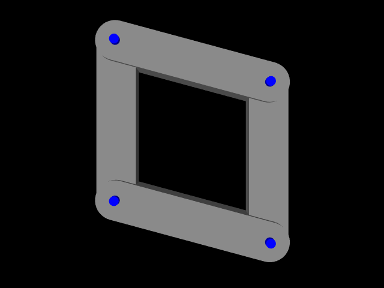
\includegraphics[]{images/FourBarLinkage}
\else
 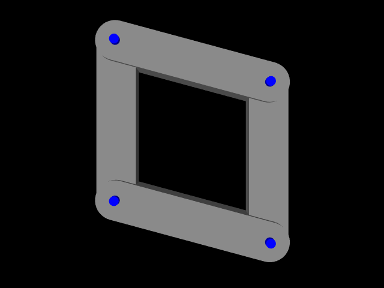
\includegraphics[width=3.75in]{images/FourBarLinkage}
\fi
\end{center}
\caption{FourBarLinkage model, several steps into the simulation.}
\label{FourBarLinkage:fig}
\end{figure}

To model a four-bar in ArtiSynth presently requires adding compliance
to the hinge joints. An example of this is defined by the demo program
%
\begin{verbatim}
  artisynth.demos.tutorial.FourBarLinkage
\end{verbatim}
%
shown in Figure \ref{FourBarLinkage:fig}.
The code for the {\tt build()} method and a couple of supporting
methods is given below:
\lstset{numbers=left}
\iflatexml
%% Hack: latexml lstinputlisting doesn't handle firstline correctly 
  \lstset{firstnumber={-25}}
  \lstinputlisting[firstline=1,lastline=73]{../../src/artisynth/demos/tutorial/FourBarLinkage.java}
  \lstset{firstnumber={1}}
\else
  \lstinputlisting[firstline=27,lastline=99]{../../src/artisynth/demos/tutorial/FourBarLinkage.java}
\fi
\lstset{numbers=none}
Two helper methods are used to construct the model: {\tt createLink()}
(lines 6-17), and {\tt createJoint()} (lines 23-36).  {\tt
createLink()} makes the individual rigid bodies used to build the
linkage: a mesh is produced defining the body's shape (a box with
rounded ends), and then passed to the
\javaclass[artisynth.core.mechmodels]{RigidBody}
{\tt createFromMesh()} method which creates the body and sets its
inertia according to a specified density. The body's pose is then set
so as to center it at $(x, 0, z)$ while rotating it about the $y$ axis
by the angle {\tt deg} (in degrees). The completed body is then added to the
{\tt MechModel} {\tt mech} and returned.

The second helper method, {\tt createJoint()}, connects two rigid
bodies ({\tt link0} and {\tt link1}) together using a {\tt
HingeJoint}. Because we know the location of the joint in
body-relative coordinates, it is easier to create the joint using the
transforms $\T_{CA}$ and $\T_{DB}$ instead of $\T_{DW}$: $\T_{CA}$
locates the joint at the top end of {\tt link0}, at $(0, 0, 0.5)$,
with the $z$ axis parallel to the body's $y$ axis, while $\T_{DB}$
similarly locates the joint at the bottom of {\tt link1}.  After the
joint is created and added to the {\tt MechModel}, its render
properties are set so that its axis drawn as a blue cylinder.

The {\tt build()} method itself begins by creating a {\tt MechModel}
and setting damping parameters for the rigid bodies (lines
40-43). Next, {\tt createLink()} is used to create and store the four
links (lines 46-50), and the left bar is attached to ground by making
it non-dynamic (line 52). The links are then connected together using
joints created by {\tt createJoint()} (lines 55-59). Finally, uniform
compliance and damping values are set for each of the joint's
bilateral constraints, using the {\tt setCompliance()} and {\tt
setDamping()} methods (lines 63-72). Values are set for the first five
constraints, since for a {\tt HingeJoint} these are the bilateral
constraints. The compliance value of $C = 10^{-6}$ was found
experimentally to be low enough so as to not cause noticeable
deflections in the joints. Given $C$ and an
average mass of around $M = 150$ for each link pair,
(\ref{constraintDamping:eqn}) suggests the damping factor of $D =
25000$. Note that for this example, very similar settings could be
achieved by simply calling
%
\begin{lstlisting}[]
  for (int i=0; i<joints.length; i++) {
     joints[i].setLinearCompliance (0.000001);
     joints[i].setRotaryCompliance (0.000001);
  }
\end{lstlisting}
%
In principle, we only need to set compliance for the constraints that
are redundant, but it can sometimes be difficult to determine exactly
which these are. Also, different values are often needed for linear
and rotary constraints; that is not necessary here because the
links have unit length and so the linear and rotary units have similar
scales.

\subsection{Rendering joints}
\label{RenderingJoints:sec}

Most joints provide a means to render themselves in order to provide a
graphical representation of their position and configuration.  Control
over this is achieved by setting various properties in the joint
component, including both specialized properties and the standard
render properties (Section \ref{RenderProperties:sec}) used by all
renderable components.

All joints which are subclasses of
\javaclass[artisynth.core.mechmodels]{JointBase} support rendering of
both their C and D coordinate frames, through the properties {\sf
drawFrameC}, {\sf drawFrameD}, and {\sf axisLength}.  The first two
properties are of the type
\javaclass[maspack.render]{Renderer\$AxisDrawStyle} (described
in detail in Section \ref{rigidBodyRendering:sec}), and can be set to
{\tt LINE} or {\tt ARROW} to enable the coordinate axes to be drawn
either as lines or solid arrows. The {\sf axisLength} property has
type {\tt double} and specifies the length with which the axes are
drawn. As with all properties, these properties can be set either in
the GUI, or in code using accessor methods supplied by the joint:
% method table
\begin{lstlisting}[]
  void setAxisLength (double l)
  double getAxisLength()

  void setDrawFrameC (AxisDrawStyle style)
  (AxisDrawStyle getDrawFrameC()

  void setDrawFrameD (AxisDrawStyle style)
  (AxisDrawStyle getDrawFrameD()
\end{lstlisting}
%

Another pair of properties used by several joints is {\sf shaftLength}
and {\sf shaftRadius}, which specify the length and radius used to
draw shaft or axis structures associated with the joint.  These are
rendered as solid cylinders, using the color indicated by the {\sf
faceColor} rendering property.  The default value of both properties
is 0; if {\sf shaftLength} is 0, then the structures are not drawn,
while if {\sf shaftRadius} is 0, a default value proportional to {\sf
shaftLength} is used. For example, to enable rendering of a blue shaft
along the rotation axis of a hinge joint, one may use the code
fragment
%
\begin{lstlisting}[]
  HingeJoint joint;
  ...

  joint.setShaftLength (0.5); // set shaft dimensions
  joint.setShaftRadius (0.05);
  RenderProps.setFaceColor (joint, Color.BLUE); // set the color
\end{lstlisting}
%
As another example, to enable rendering of a green ball about the
center of a spherical joint, one may use the fragment
%
\begin{lstlisting}[]
  SphericalJoint joint;
  ...

  joint.setJointRadius (0.02); // set the ball size
  RenderProps.setFaceColor (joint, Color.GREEN); // set the color
\end{lstlisting}
%

Specific joints may define additional properties to control how they
are rendered.

\section{Joint components}
\label{JointTypes:sec}

ArtiSynth supplies a number of basic joints and connectors in the package {\tt
artisynth.core.mechmodels}, the most common of which are described
here. 

Many of the descriptions are associated with a demonstration model,
named {\tt XXXJointDemo}, where {\tt XXX} is the joint type.  These
demos are located in the package {\tt artisynth.demos.mech}, and can
be loaded by selecting {\sf All demos > mech > XXXJointDemo} from the
{\sf Models} menu. When run, they can be interactively controlled,
using either the pull tool (see the section ``Pull Manipulation'' in
the \artisynthManual{uiguide}{ArtiSynth User Interface Guide}), or the
interactive control panel. The control panel allows the adjustment of
coordinate values and ranges (if supported), some of the render
properties, and the different {\sf compliance} and {\sf damping}
properties (Section \ref{JointCompliance:sec}).  One can inspect the
source code for each demo in its {\tt .java} file located in the
folder {\tt <ARTISYNTH\_HOME>/src/artisynth/demos/mech}.

\subsection{Hinge joint}
\label{HingeJoint:sec}

\begin{figure}[h]
\begin{center}
\begin{tabular}{c@{\hskip .5in}c}
 \iflatexml
   \includegraphics[width=2.333in]{images/hingeJoint}&
   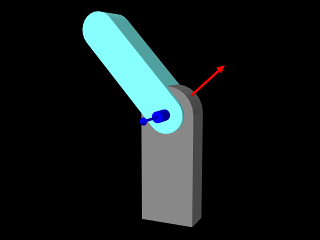
\includegraphics[width=3.1in]{images/HingeJointDemo}\\
 \else
   \includegraphics[width=1.75in]{images/hingeJoint}&
   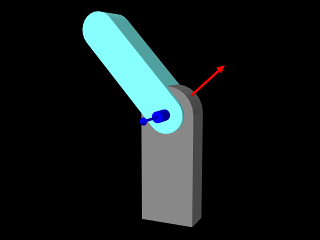
\includegraphics[width=2.333in]{images/HingeJointDemo}\\
 \fi
\end{tabular}
\end{center}
\caption{Coordinate frames (left) and demo model (right)
for the hinge joint.}
\label{HingeJoint:fig}
\end{figure}

The \javaclass[artisynth.core.mechmodels]{HingeJoint} 
(Figure \ref{HingeJoint:fig}) is a 1 DOF joint that
constrains motion between frames C and D to a simple rotation about
the $z$ axis of D.  It implements six constraints and one coordinate
$\theta$ (Table \ref{HingeConstraints:tbl}), to which the joint transform
$\T_{CD}$ is related by
%
\begin{equation*}
\T_{CD} = \matl
\cos(\theta) & -\sin(\theta) & 0 & 0 \\
\sin(\theta) &  \cos(\theta) & 0 & 0 \\
0 & 0 & 1 & 0 \\
0 & 0 & 0 & 1 
\matr.
\end{equation*}
%
The value and ranges for $\theta$ are exported by the properties {\sf
theta} and {\sf thetaRange}, and the $\theta$ coordinate index is
defined by the constant {\tt THETA\_IDX}.  For rendering, the
properties {\sf shaftLength} and {\sf shaftRadius} control the size of
a shaft drawn about the rotation axis, using the {\sf faceColor}
rendering property.  A demo is provided by \\ {\tt
artisynth.demos.mech.HingeJointDemo}.

In addition to the standard constructors described in
Section \ref{CreatingJoints:sec},
% method table
\begin{lstlisting}[]
  HingeJoint (bodyA, bodyB, originD, zaxis)
\end{lstlisting}
%
creates a hinge joint with a specified origin and $z$ axis direction
for frame D (in world coordinates), and frames C and D coincident.

\begin{table}[h]
\centering
\begin{tabular}{|l|l|l|}
\hline
Index & type/name & description \\
\hline
0 & bilateral & restricts translation along $x$ \\
1 & bilateral & restricts translation along $y$ \\
2 & bilateral & restricts translation along $z$ \\
3 & bilateral & restricts rotation about $x$ \\
4 & bilateral & restricts rotation about $y$ \\
5 & unilataral & enforces limits on $\theta$ \\
\hline
\hline
0 & $\theta$ & counter-clockwise rotation of $C$ about the $z$ axis \\
\hline
\end{tabular}
\caption{Constraints (top) and coordinates (bottom) for the hinge joint.}
\label{HingeConstraints:tbl}
\end{table}

\subsection{Slider joint}

\begin{figure}[h]
\begin{center}
\begin{tabular}{c@{\hskip .5in}c}
 \iflatexml
   \includegraphics[width=2.333in]{images/sliderJoint}&
   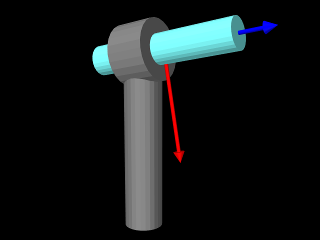
\includegraphics[width=3.1in]{images/SliderJointDemo}\\
 \else
   \includegraphics[width=1.75in]{images/sliderJoint}&
   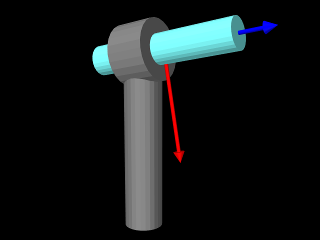
\includegraphics[width=2.333in]{images/SliderJointDemo}\\
 \fi
\end{tabular}
\end{center}
\caption{Coordinate frames (left) and demo model (right)
for the slider joint.}
\label{SliderJoint:fig}
\end{figure}

The \javaclass[artisynth.core.mechmodels]{SliderJoint} 
(Figure \ref{SliderJoint:fig}) is a 1 DOF joint
that constrains motion between frames C and D to a simple translation
along the $z$ axis of D.  It implements six constraints and one
coordinate $z$ (Table \ref{SliderConstraints:tbl}), to which the joint
transform $\T_{CD}$ is related by
%
\begin{equation*}
\T_{CD} = \matl
1 & 0 & 0 & 0 \\
0 & 1 & 0 & 0 \\
0 & 0 & 1 & z \\
0 & 0 & 0 & 1 
\matr.
\end{equation*}
%\
The value and ranges for $z$ are exported by the properties {\sf z}
and {\sf zRange}, and the $z$ coordinate index is defined by the
constant {\tt Z\_IDX}.  For rendering, the properties {\sf
shaftLength} and {\sf shaftRadius} control the size of a shaft drawn
about the sliding axis, using the {\sf faceColor} rendering property.
A demo is provided by {\tt artisynth.demos.mech.SliderJointDemo}.

In addition to the standard constructors described in
Section \ref{CreatingJoints:sec},
% method table
\begin{lstlisting}[]
  SliderJoint (bodyA, bodyB, originD, zaxis)
\end{lstlisting}
%
creates a slider joint with a specified origin and $z$ axis direction
for frame D (in world coordinates), and frames C and D coincident.

\begin{table}[h]
\centering
\begin{tabular}{|l|l|l|}
\hline
Index & type/name & description \\
\hline
0 & bilateral & restricts translation along $x$ \\
1 & bilateral & restricts translation along $y$ \\
2 & bilateral & restricts rotation about $x$ \\
3 & bilateral & restricts rotation about $y$ \\
4 & bilateral & restricts rotation about $z$ \\
5 & unilataral & enforces limits on the $z$ coordinate \\
\hline
\hline
0 & $z$ & translation of $C$ along the $z$ axis \\
\hline
\end{tabular}
\caption{Constraints (top) and coordinates (bottom) for the slider joint.}
\label{SliderConstraints:tbl}
\end{table}

\subsection{Cylindrical joint}

\begin{figure}[h]
\begin{center}
\begin{tabular}{c@{\hskip .5in}c}
 \iflatexml
   \includegraphics[width=2.333in]{images/cylindricalJoint}&
   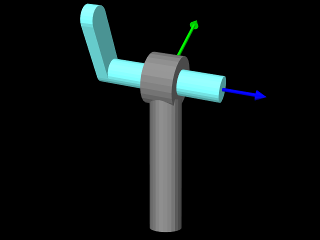
\includegraphics[width=3.1in]{images/CylindricalJointDemo}\\
 \else
   \includegraphics[width=1.75in]{images/cylindricalJoint}&
   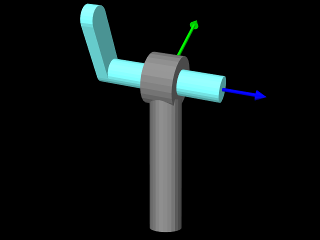
\includegraphics[width=2.333in]{images/CylindricalJointDemo}\\
 \fi
\end{tabular}
\end{center}
\caption{Coordinate frames (left) and demo model (right)
for the cylindrical joint.}
\label{CylindricalJoint:fig}
\end{figure}

The \javaclass[artisynth.core.mechmodels]{CylindricalJoint} 
(Figure \ref{CylindricalJoint:fig}) is a 2 DOF
joint that constrains motion between frames C and D to translation and
rotation along and about the $z$ axis of D.  It implements six
constraints and two coordinates $z$ and $\theta$
(Table \ref{CylindricalConstraints:tbl}), to which the joint transform
$\T_{CD}$ is related by
%
\begin{equation*}
\T_{CD} = \matl
\cos(\theta) & -\sin(\theta) & 0 & 0 \\
\sin(\theta) &  \cos(\theta) & 0 & 0 \\
0 & 0 & 1 & z \\
0 & 0 & 0 & 1 
\matr.
\end{equation*}
%\
The value and ranges for $z$ and $\theta$ are exported by the
properties {\sf z}, {\sf theta}, {\sf zRange} and {\sf thetaRange},
and the coordinate indices are defined by the constants {\tt Z\_IDX}
and {\tt THETA\_IDX}. For rendering, the properties {\sf shaftLength}
and {\sf shaftRadius} control the size of a shaft drawn about the
sliding/rotation axis, using the {\sf faceColor} rendering property.
A demo is provided by {\tt artisynth.demos.mech.CylindricalJointDemo}.

In addition to the standard constructors described in
Section \ref{CreatingJoints:sec},
% method table
\begin{lstlisting}[]
  CylindricalJoint (bodyA, bodyB, originD, zaxis)
\end{lstlisting}
%
creates a cylindrical joint with a specified origin and $z$ axis direction
for frame D (in world coordinates), and frames C and D coincident.

\begin{table}[h]
\centering
\begin{tabular}{|l|l|l|}
\hline
Index & type/name & description \\
\hline
0 & bilateral & restricts translation along $x$ \\
1 & bilateral & restricts translation along $y$ \\
2 & bilateral & restricts rotation about $x$ \\
3 & bilateral & restricts rotation about $y$ \\
4 & unilataral & enforces limits on the $z$ coordinate \\
5 & unilataral & enforces limits on the $\theta$ coordinate \\
\hline
\hline
0 & $z$ & translation of $C$ along the $z$ axis \\
1 & $\theta$ & rotation of $C$ about the $z$ axis \\
\hline
\end{tabular}
\caption{Constraints (top) and coordinates (bottom) for the cylindrical joint.}
\label{CylindricalConstraints:tbl}
\end{table}

\subsection{Slotted hinge joint}
\label{SlottedHingeJoint:sec}

\begin{figure}[h]
\begin{center}
\begin{tabular}{c@{\hskip .5in}c}
 \iflatexml
   \includegraphics[width=2.333in]{images/slottedHingeJoint}&
   \includegraphics[width=3.1in]{images/SlottedHingeJointDemo}\\
 \else
   \includegraphics[width=1.75in]{images/slottedHingeJoint}&
   \includegraphics[width=2.333in]{images/SlottedHingeJointDemo}\\
 \fi
\end{tabular}
\end{center}
\caption{Coordinate frames (left) and demo model (right)
for the slotted hinge joint.}
\label{SlottedHingeJoint:fig}
\end{figure}

The \javaclass[artisynth.core.mechmodels]{SlottedHingeJoint} 
(Figure \ref{SlottedHingeJoint:fig}) is
a 2 DOF joint that constrains motion between frames C and D to
translation along the $x$ axis and rotation about the $z$ axis of D.
It implements six constraints and two coordinates $x$ and $\theta$
(Table \ref{SlottedHingeConstraints:tbl}), to which the joint
transform $\T_{CD}$ is related by
%
\begin{equation}
\T_{CD} = \matl
\cos(\theta) & -\sin(\theta) & 0 & x \\
\sin(\theta) &  \cos(\theta) & 0 & 0 \\
0 & 0 & 1 & 0 \\
0 & 0 & 0 & 1 
\matr.
\label{SlottedHingeTCD:eqn}
\end{equation}
%\
The value and ranges for $x$ and $\theta$ are exported by the
properties {\sf x}, {\sf theta}, {\sf xRange} and {\sf thetaRange},
and the coordinate indices are defined by the constants {\tt X\_IDX}
and {\tt THETA\_IDX}. For rendering, the properties {\sf shaftLength}
and {\sf shaftRadius} control the size of a shaft drawn about the
rotation axis, while {\sf slotWidth} and {\sf slotDepth} control the
width and depth of a slot drawn along the sliding ($x$) axis; both are
drawn using the {\sf faceColor} rendering property. When rendering the
slot, its bounds along the $x$ axis are set to {\sf xRange} by
default. However, this may be too large, particularly if {\sf xRange}
is unbounded. As an alternate, the property {\sf slotRange} will be
used instead if its range (i.e., the upper bound minus the lower
bound) exceeds 0.  A demo of {\tt SlottedHingeJoint} is provided by
{\tt artisynth.demos.mech.SlottedHingeJointDemo}.

In addition to the standard constructors described in
Section \ref{CreatingJoints:sec},
% method table
\begin{lstlisting}[]
  SlottedHingeJoint (bodyA, bodyB, originD, zaxis)
\end{lstlisting}
%
creates a slotted hinge joint with a specified origin and $z$ axis direction
for frame D (in world coordinates), and frames C and D coincident.

\begin{table}[h]
\centering
\begin{tabular}{|l|l|l|}
\hline
Index & type/name & description \\
\hline
0 & bilateral & restricts translation along $y$ \\
1 & bilateral & restricts translation along $z$ \\
2 & bilateral & restricts rotation about $x$ \\
3 & bilateral & restricts rotation about $y$ \\
4 & unilataral & enforces limits on the $x$ coordinate \\
5 & unilataral & enforces limits on the $\theta$ coordinate \\
\hline
\hline
0 & $x$ & translation of $C$ along the $x$ axis \\
1 & $\theta$ & rotation of $C$ about the $z$ axis \\
\hline
\end{tabular}
\caption{Constraints (top) and coordinates (bottom) for the slotted hinge joint.}
\label{SlottedHingeConstraints:tbl}
\end{table}

\subsection{Universal joint}

\begin{figure}[h]
\begin{center}
\begin{tabular}{c@{\hskip .5in}c}
 \iflatexml
   \includegraphics[width=2.333in]{images/universalJoint}&
   \includegraphics[width=3.1in]{images/UniversalJointDemo}\\
 \else
   \includegraphics[width=1.75in]{images/universalJoint}&
   \includegraphics[width=2.333in]{images/UniversalJointDemo}\\
 \fi
\end{tabular}
\end{center}
\caption{Coordinate frames (left) and demo model (right)
for the universal joint.}
\label{UniversalJoint:fig}
\end{figure}

\begin{table}[h]
\centering
\begin{tabular}{|l|l|l|}
\hline
Index & type/name & description \\
\hline
0 & bilateral & restricts translation along $x$ \\
1 & bilateral & restricts translation along $y$ \\
2 & bilateral & restricts translation along $z$ \\
3 & bilateral & restricts rotation about the final $x$ axis of C \\
4 & unilataral & enforces limits on the roll coordinate \\
5 & unilataral & enforces limits on the pitch coordinate \\
\hline
\hline
0 & $\theta$ (roll) & first rotation of $C$ about the $z$ axis of D \\
1 & $\phi$ (pitch) & second rotation of $C$ about the rotated $y'$ axis \\
\hline
\end{tabular}
\caption{Constraints (top) and coordinates (bottom) for the universal joint.}
\label{UniversalConstraints:tbl}
\end{table}

The \javaclass[artisynth.core.mechmodels]{UniversalJoint} 
(Figure \ref{UniversalJoint:fig}) is a 2 DOF joint
that allows C two rotational degrees of freedom with respect to D: a
{\it roll} rotation $\theta$ about D's $z$ axis, followed by a {\it
pitch} rotation $\phi$ about the rotated $y'$ axis. It implements six
constraints and the two coordinates $\theta$ and $\phi$
(Table \ref{UniversalConstraints:tbl}), to which the joint transform
$\T_{CD}$ is related by
%
\begin{equation*}
\T_{CD} = \matl
\Cr \Cp & -\Sr & \Cr \Sp & 0 \\
\Sr \Cp & \Cr & \Sr \Sp & 0 \\
-\Sp & 0 & \Cp & 0 \\
0 & 0 & 0 & 1 
\matr,
\end{equation*}
%\
where 
%
\begin{equation*}
\Cr \equiv \cos(\theta),\; 
\Sr \equiv \sin(\theta),\;
\Cp \equiv \cos(\phi),\;
\Sp \equiv \sin(\phi).
\end{equation*}
%
The value and ranges for $\theta$ and $\phi$ are exported by the
properties {\sf roll}, {\sf pitch}, {\sf rollRange} and {\sf
pitchRange}, and the coordinate indices are defined by the constants
{\tt ROLL\_IDX} and {\tt PITCH\_IDX}.  

For rendering, the properties {\sf shaftLength} and {\sf shaftRadius} control
the size of shafts drawn about the roll and pitch axes, while {\sf jointRadius}
specifies the radius of a ball drawn around the origin of D; both are drawn
using the {\sf faceColor} rendering property. It is also
possible to add a rendering mesh, using the methods:
% method table
\begin{lstlisting}[]
  void setRenderMesh (PolygonalMesh mesh)
  PolygonalMesh getRenderMesh()
\end{lstlisting}
%
If present, the rendering mesh is rendered in the intermediate
frame between D and C, i.e., D rotated about $z$ by $\theta$.
Rendering is controlled by the face rendering properties (
{\sf faceStyle}, {\sf faceColor}, etc.).

A demo is provided by {\tt artisynth.demos.mech.UniversalJointDemo}.

\subsection{Skewed universal joint}

The \javaclass[artisynth.core.mechmodels]{SkewedUniversalJoint}
(Figure \ref{SkewedUniversalJoint:fig}) is a version of the universal
joint in which the pitch axis is skewed relative to its nominal direction
by an angle $\alpha$. More precisely, let $x'$ and $y'$ be the $x$ and
$y$ axes of C after the initial roll rotation. For a regular universal
joint, the pitch axis is $y'$, whereas for a skewed universal joint it
is $y'$ rotated by $\alpha$ clockwise about $x'$. The joint still has
2 DOF, but the space of allowed rotations is reduced.

\begin{figure}[hhh]
\begin{center}
\begin{tabular}{c@{\hskip .5in}c}
 \iflatexml
   \includegraphics[width=2.333in]{images/skewedUniversalJoint}&
   \includegraphics[width=3.1in]{images/SkewedUniversalJointDemo}\\
 \else
   \includegraphics[width=1.75in]{images/skewedUniversalJoint}&
   \includegraphics[width=2.333in]{images/SkewedUniversalJointDemo}\\
 \fi
\end{tabular}
\end{center}
\caption{Left: diagram for a skewed universal joint, showing the 
pitch axis (dotted line) skewed by an angle $\alpha$ relative to its
nominal direction along the $y'$ axis. Right: demo model with skew
angle of $30^\circ$.}
\label{SkewedUniversalJoint:fig}
\end{figure}

The constraints and the coordinates are the same as for the universal
joint, although the relationship between $\T_{CD}$ is now more complicated.
With $\Cr$, $\Sr$, $\Cp$, and $\Sp$ defined as for the universal
joint, $\T_{CD}$ is given by
%
\begin{equation*}
\T_{CD} = \matl
\Cr\Cp - \Sr\Sa\Sp & -\Sr\beta - \Sa\Cr\Sp & \Ca(\Cr\Sp - \Sa\Sr\Vp) & 0 \\
\Sr\Cp + \Cr\Sa\Sp & \Cr\beta - \Sa\Sr\Sp  & \Ca(\Sr\Sp + \Sa\Cr\Vp) & 0 \\
-\Ca \Sp           & \Ca\Sa\Vp             &  \Sa^2 + \Ca^2\Cp       & 0 \\
0 & 0 & 0 & 1 
\matr,
\end{equation*}
%\
where 
%
\begin{equation*}
\Ca \equiv \cos(\alpha), \quad
\Sa \equiv \sin(\alpha), \quad
\Vp \equiv 1 - \Cp, \quad \beta \equiv \Ca^2 + \Sa^2 \Cp.
\end{equation*}
%
Rendering is controlled using the properties {\sf shaftLength}, {\sf
shaftRadius} and {\sf jointRadius} in the same way as for the {\tt
UniversalJoint}.  A demo is provided by calling {\tt
artisynth.demos.mech.UniversalJointDemo} with the model arguments {\tt
-skew <angDeg>}, where {\tt <angDeg>} is the desired skew angle in
degrees.

Constructors for skewed universal joints take the standard forms
described in Section \ref{CreatingJoints:sec}, with an additional
argument at the end indicating the skew angle:
% method table
\begin{lstlisting}[]
  SkewedUniveralJoint (bodyA, TCA, bodyB, TCB, skewAngle)

  SkewedUniveralJoint (bodyA, bodyB, TDW, skewAngle)

  SkewedUniveralJoint (bodyA, bodyB, TCW, TDW, skewAngle)
\end{lstlisting}
%
In addition, the constructor
% method table
\begin{lstlisting}[]
  SkewedUniveralJoint (bodyA, bodyB, originD, rollAxis, pitchAxis)
\end{lstlisting}
%
creates a skewed universal joint specifying the origin of frame D
together with the directions of the roll and pitch axes (in world
coordinates). Frames C and D are coincident and the skew angle is
inferred from the angle between the axes.

\subsection{Gimbal joint}

\begin{figure}[h]
\begin{center}
\begin{tabular}{c@{\hskip .5in}c}
 \iflatexml
   \includegraphics[width=2.333in]{images/sphericalJoint2}&
   \includegraphics[width=3.1in]{images/GimbalJointDemo}\\
 \else
   \includegraphics[width=1.75in]{images/sphericalJoint2}&
   \includegraphics[width=2.333in]{images/GimbalJointDemo}\\
 \fi
\end{tabular}
\end{center}
\caption{Coordinate frames (left; rotation angles not shown) 
and demo model (right) for the gimbal joint.}
\label{GimbalJoint:fig}
\end{figure}

The \javaclass[artisynth.core.mechmodels]{GimbalJoint}
(Figure \ref{GimbalJoint:fig}) is a 3 DOF spherical joint that anchors
the origins of C and D together but otherwise allows C complete
rotational freedom. The rotational degrees of freedom are
parameterized by three roll-pitch-yaw angles, denoted by
$\theta, \phi, \psi$, which define a rotation $\theta$ about D's $z$
axis, followed by a second rotation $\phi$ about the rotated $y'$
axis, followed by a third rotation $\psi$ about the final $x''$ axis.
It implements six constraints and the three coordinates
$\theta, \phi, \psi$ (Table \ref{GimbalConstraints:tbl}), to which the
joint transform $\T_{CD}$ is related by
%
\begin{equation*}
\T_{CD} = \matl
\Cr \Cp & \Cr \Sp \Sy - \Sr \Cy & \Cr \Sp \Cy + \Sr \Sy & 0 \\
\Sr \Cp & \Sr \Sp \Sy + \Cr \Cy & \Sr \Sp \Cy - \Cr \Sy & 0 \\
-\Sp & \Cp \Sy & \Cp \Cy & 0 \\
0 & 0 & 0 & 1 
\matr,
\end{equation*}
%\
where 
%
\begin{equation*}
\Cr \equiv \cos(\theta),\;
\Sr \equiv \sin(\theta),\;
\Cp \equiv \cos(\phi),\;
\Sp \equiv \sin(\phi),\;
\Cy \equiv \cos(\psi),\;
\Sy \equiv \sin(\psi).
\end{equation*}
%
The value and ranges for $\theta, \phi, \psi$ are exported by the
properties {\sf roll}, {\sf pitch}, {\sf yaw}, {\sf rollRange}, {\sf
pitchRange}, and {\sf yawRange}, and the coordinate indices are
defined by the constants {\tt ROLL\_IDX}, {\tt PITCH\_IDX}, and {\tt
YAW\_IDX}. For rendering, the property {\sf jointRadius} specifies the
radius of a ball drawn around the origin of D, using the {\sf
faceColor} rendering property.  A demo is provided by {\tt
artisynth.demos.mech.GimbalJointDemo}.

In addition to the standard constructors described in
Section \ref{CreatingJoints:sec},
% method table
\begin{lstlisting}[]
  GimbalJoint (bodyA, bodyB, originD)
\end{lstlisting}
%
creates a gimbal joint with a specified origin for frame D (in world
coordinates), and frames C and D coincident and world aligned.

\begin{sideblock}
The constraints implementing {\tt GimbalJoint} are designed so that it
is immune to {\it gimbal lock}, in which a degree of freedom is lost
when $\phi = \pm \pi/2$. However, the coordinate values themselves are
not immune to this singularity, and neither are the unilateral
constraints which enforce limits on their values. Therefore, if
coordinate limits are implemented, the joint should be deployed so as try
and avoid pitch values near $\pm \pi/2$.
\end{sideblock}

\begin{table}[h]
\centering
\begin{tabular}{|l|l|l|}
\hline
Index & type/name & description \\
\hline
0 & bilateral & restricts translation along $x$ \\
1 & bilateral & restricts translation along $y$ \\
2 & bilateral & restricts translation along $z$ \\
3 & unilataral & enforces limits on the roll coordinate \\
4 & unilataral & enforces limits on the pitch coordinate \\
5 & unilataral & enforces limits on the yaw coordinate \\
\hline
\hline
0 & $\theta$ (roll) & first rotation of $C$ about the $z$ axis of D \\
1 & $\phi$ (pitch) & second rotation of $C$ about the rotated $y'$ axis \\
2 & $\psi$ (yaw) & third rotation of $C$ about the final $x''$ axis \\
\hline
\end{tabular}
\caption{Constraints (top) and coordinates (bottom) for the gimbal joint.}
\label{GimbalConstraints:tbl}
\end{table}

\subsection{Spherical joint}

\begin{figure}[h]
\begin{center}
\begin{tabular}{c@{\hskip .5in}c}
 \iflatexml
   \includegraphics[width=2.333in]{images/sphericalJoint3}&
   \includegraphics[width=3.1in]{images/SphericalJointDemo}\\
 \else
   \includegraphics[width=1.75in]{images/sphericalJoint3}&
   \includegraphics[width=2.333in]{images/SphericalJointDemo}\\
 \fi
\end{tabular}
\end{center}
\caption{Left: coordinate frames of the spherical joint, showing the
tilt angle $\phi$ between the $z$ axes of C and D.  Right: demo model
for the spherical joint.}
\label{SphericalJoint:fig}
\end{figure}

The \javaclass[artisynth.core.mechmodels]{SphericalJoint} (Figure
\ref{SphericalJoint:fig}) is a 3 DOF spherical joint that, like
\javaclass[artisynth.core.mechmodels]{GimbalJoint}, anchors the
origins of C and D together but otherwise allows C complete rotational
freedom. {\tt SphericalJoint} does not implement any coordinates, and
so is conceptually more like a {\it ball} joint.  However, it does
provide two choices for limiting its rotation:

\begin{itemize}

\item A limit on the {\it tilt} angle $\phi$ between
the $z$ axes of D and C, such that
%
\begin{equation}
\phi \le \phi_\text{max}.
\end{equation}
%
This is intended to emulate the limit imposed by a ball joint socket.

\item A limit on the total rotation, defined as follows: Let $(\u, \theta)$
be the axis-angle representation of the rotation matrix of $\T_{CD}$,
normalized such that $\theta \ge 0$ and $\|u\| = 1$, and let
$\r_\text{max}$ be a three-vector giving maximum rotation angles with
$x$, $y$, and $z$ components. Then $\theta$ is constrained by
%
\begin{equation}
\theta \le \| \r_\text{max} \circ \u \|,
\end{equation}
%
where $\circ$ denotes the element-wise product. If the components of
$\r_\text{max}$ are set to a uniform value $\theta_\text{max}$, this
simplifies to $\theta \le \theta_\text{max}$.

\end{itemize}

These limits can be enabled by setting the joint's properties {\sf
isTiltLimited} and {\sf isRotationLimited}, respectively, where
enabling one disables the other. The limit values $\phi_\text{max}$
and $\r_\text{max}$ are managed using the properties {\sf maxTilt} and
{\sf maxRotation}, and setting either automatically enables tilt or
rotation limiting, as appropriate. Finally, the tilt angle $\phi$ can
be queried using the (read-only) {\sf tilt} property.  For rendering,
the property {\sf jointRadius} specifies the radius of a ball drawn
around the origin of D, using the {\sf faceColor} rendering
property. A demo of the {\tt SphericalJoint} is provided by {\tt
artisynth.demos.mech.SphericalJointDemo}.

In addition to the standard constructors described in
Section \ref{CreatingJoints:sec},
% method table
\begin{lstlisting}[]
  SphericalJoint (bodyA, bodyB, originD)
\end{lstlisting}
%
creates a spherical joint with a specified origin for frame D (in
world coordinates), and frames C and D coincident and world aligned.

\begin{sideblock}
One should use the rotation limit with some caution, as the
orientations which it prohibits can be somewhat hard to predict,
particularly when $\r_\text{max}$ has non-uniform values.
\end{sideblock}

\begin{table}[h]
\centering
\begin{tabular}{|l|l|l|}
\hline
Index & type/name & description \\
\hline
0 & bilateral & restricts translation along $x$ \\
1 & bilateral & restricts translation along $y$ \\
2 & bilateral & restricts translation along $z$ \\
3 & unilataral & enforces either the ``tilt'' or ``rotation'' limits\\
\hline
\end{tabular}
\caption{Constraints for the spherical joint.}
\label{SphericalConstraints:tbl}
\end{table}

\subsection{Planar joint}

\begin{figure}[h]
\begin{center}
\begin{tabular}{c@{\hskip .5in}c}
 \iflatexml
   \includegraphics[width=2.333in]{images/planarJoint}&
   \includegraphics[width=3.1in]{images/PlanarJointDemo}\\
 \else
   \includegraphics[width=1.75in]{images/planarJoint}&
   \includegraphics[width=2.333in]{images/PlanarJointDemo}\\
 \fi
\end{tabular}
\end{center}
\caption{Coordinate frames (left) and demo model (right)
for the planar joint.}
\label{PlanarJoint:fig}
\end{figure}

The \javaclass[artisynth.core.mechmodels]{PlanarJoint} 
(Figure \ref{PlanarJoint:fig}) is a 3 DOF
joint that constrains C to translation in the $x$-$y$ plane 
and rotation about the $z$ axis of D.  It implements six
constraints and three coordinates $x$, $y$ and $\theta$
(Table \ref{PlanarConstraints:tbl}), to which the joint transform
$\T_{CD}$ is related by
%
\begin{equation*}
\T_{CD} = \matl
\cos(\theta) & -\sin(\theta) & 0 & x \\
\sin(\theta) &  \cos(\theta) & 0 & y \\
0 & 0 & 1 & 0 \\
0 & 0 & 0 & 1 
\matr.
\end{equation*}
%\
The value and ranges for $x$, $y$ and $\theta$ are exported by the
properties {\sf x}, {\sf y}, {\sf theta}, {\sf xRange}, {\sf yRange}
and {\sf thetaRange}, and the coordinate indices are defined by the
constants {\tt X\_IDX}, {\tt Y\_IDX} and {\tt THETA\_IDX}.  
A planar joint can be rendered as a square centered on the origin
of D, using face rendering properties and with a size given by the
{\sf planeSize} property. For example,
%
\begin{lstlisting}[]
  PlanarJoint joint;
  ...
  joint.setPlaneSize (5.0);
  RenderProps.setFaceColor (joint, Color.LIGHT_GRAY);
\end{lstlisting}
%
will cause {\tt joint} to be drawn as a light gray square with size
5.0. The default value of {\sf planeSize} is 0, so drawing the plane
is disabled by default. Also, the default {\sf faceStyle} rendering
property for {\tt PlanarConnector} is set to {\tt FRONT\_AND\_BACK},
so that the plane (when drawn) can be seen from both sides.  A shaft
about the rotation axis can also be drawn, as controlled by the
properties {\sf shaftLength} and {\sf shaftRadius} and using the {\sf
faceColor} rendering property.  A demo is provided by {\tt
artisynth.demos.mech.PlanarJointDemo}.

In addition to the standard constructors described in
Section \ref{CreatingJoints:sec},
% method table
\begin{lstlisting}[]
  PlanarJoint (bodyA, bodyB, originD, zaxis)
\end{lstlisting}
%
creates a planar joint with a specified origin and $z$ axis direction
for frame D (in world coordinates), and frames C and D coincident.

\begin{table}[h]
\centering
\begin{tabular}{|l|l|l|}
\hline
Index & type/name & description \\
\hline
0 & bilateral & restricts translation along $z$ \\
1 & bilateral & restricts rotation about $x$ \\
2 & bilateral & restricts rotation about $y$ \\
3 & unilataral & enforces limits on the $x$ coordinate \\
3 & unilataral & enforces limits on the $y$ coordinate \\
5 & unilataral & enforces limits on the $\theta$ coordinate \\
\hline
\hline
0 & $x$ & translation of $C$ along the $x$ axis of D \\
1 & $y$ & translation of $C$ along the $y$ axis of D \\
2 & $\theta$ & rotation of $C$ about the $z$ axis of D\\
\hline
\end{tabular}
\caption{Constraints (top) and coordinates (bottom) for the planar joint.}
\label{PlanarConstraints:tbl}
\end{table}

\subsection{Planar translation joint}

\begin{figure}[h]
\begin{center}
\begin{tabular}{c@{\hskip .5in}c}
 \iflatexml
   \includegraphics[width=2.333in]{images/planarTranslationJoint}&
   \includegraphics[width=3.1in]{images/PlanarTranslationJointDemo}\\
 \else
   \includegraphics[width=1.75in]{images/planarTranslationJoint}&
   \includegraphics[width=2.333in]{images/PlanarTranslationJointDemo}\\
 \fi
\end{tabular}
\end{center}
\caption{Coordinate frames (left) and demo model (right)
for the planar translation joint.}
\label{PlanarTranslationJoint:fig}
\end{figure}

\begin{table}[h]
\centering
\begin{tabular}{|l|l|l|}
\hline
Index & type/name & description \\
\hline
0 & bilateral & restricts translation along $z$ \\
1 & bilateral & restricts rotation about $x$ \\
2 & bilateral & restricts rotation about $y$ \\
3 & bilateral & restricts rotation about $z$ \\
4 & unilataral & enforces limits on the $x$ coordinate \\
5 & unilataral & enforces limits on the $y$ coordinate \\
\hline
\hline
0 & $x$ & translation of $C$ along the $x$ axis of D \\
1 & $y$ & translation of $C$ along the $y$ axis of D \\
\hline
\end{tabular}
\caption{Constraints (top) and coordinates (bottom) for the planar
translation joint.}
\label{PlanarTranslationConstraints:tbl}
\end{table}

The \javaclass[artisynth.core.mechmodels]{PlanarTranslationJoint} 
(Figure \ref{PlanarTranslationJoint:fig}) is a 2 DOF joint
that is the same as the planar joint without rotation:
C is restricted to translation in the $x$-$y$ plane of D.
It implements six
constraints and two coordinates $x$ and $y$
(Table \ref{PlanarTranslationConstraints:tbl}), to which the joint transform
$\T_{CD}$ is related by
%
\begin{equation*}
\T_{CD} = \matl
1 & 0 & 0 & x \\
0 & 1 & 0 & y \\
0 & 0 & 1 & 0 \\
0 & 0 & 0 & 1 
\matr.
\end{equation*}
%\
The value and ranges for $x$ and $y$ are exported by the properties
{\sf x}, {\sf y}, {\sf xRange} and {\sf yRange}, and the coordinate
indices are defined by the constants {\tt X\_IDX} and {\tt Y\_IDX}.  A
planar translation joint can be rendered as a square centered on the
origin of D, using face rendering properties and with a size given by
the {\sf planeSize} property, in the same way as described for {\tt
PlanarJoint}.  A demo is provided by {\tt
artisynth.demos.mech.PlanarJointDemo}.

In addition to the standard constructors described in
Section \ref{CreatingJoints:sec},
% method table
\begin{lstlisting}[]
  PlanarTranslationJoint (bodyA, bodyB, originD, zaxis)
\end{lstlisting}
%
creates a planar translation joint with a specified origin and $z$
axis direction for frame D (in world coordinates), and frames C and D
coincident.

\subsection{Ellipsoid joint}

The \javaclass[artisynth.core.mechmodels]{EllipsoidJoint} is a 4 DOF
joint that provides similar functionality to the ellipsoidal and
scapulothoracic joints available in OpenSim. It allows the origin of C
to slide around on the surface of an ellipsoid centered on the origin
of D, together with two additional rotational degrees of freedom.

\begin{figure}[h]
\begin{center}
\begin{tabular}{c@{\hskip .5in}c@{\hskip .5in}c}
 \iflatexml
   \includegraphics[width=2.333in]{images/ellipsoidJointS}&
   \includegraphics[width=1.8in]{images/ellipsoidJointC}&
   \includegraphics[width=2.333in]{images/EllipsoidJointDemo}
 \else
   \includegraphics[width=1.75in]{images/ellipsoidJointS}&
   \includegraphics[width=1.4in]{images/ellipsoidJointC}&
   \includegraphics[width=1.75in]{images/EllipsoidJointDemo}
 \fi
\end{tabular}
\end{center}
\caption{Ellipsoidal joint. Left: frame relationships between
D and S (blue). Middle: frame relationships between S and C (blue).
Right: the demo model {\tt EllipsoidJointDemo}, with
$\psi$, $\gamma$, $\theta$ and $\phi$ set to $45^\circ$, $30^\circ$,
$-40^\circ$, and $20^\circ$.}
\label{EllipsoidalJoint:fig}
\end{figure}

The joint kinematics is easiest to describe in terms of an
intermediate frame S whose origin lies on the ellipsoid surface,
with its position controlled by two coordinates: a {\it longitude}
angle $\psi$, and a {\it latitude} angle $\gamma$ (Figure
\ref{EllipsoidalJoint:fig}, left). Frame C has the same origin as
S, with two additional coordinates, $\theta$ and $\phi$ which allow it
to rotate about S (Figure \ref{EllipsoidalJoint:fig}, middle).  If the
transform $\T_{SD}$ from S to D and the (rotational-only) transform
$\T_{CS}$ from C to S are given by
%
\begin{equation*}
\T_{SD} = \matl \R_{SD} & \p_{SD} \\ 0 & 1 \matr
\quad \text{and} \quad
\T_{CS} = \matl \R_{CS} & 0 \\ 0 & 1 \matr,
\end{equation*}
%
then $\T_{CD}$ is given by
%
\begin{equation*}
\T_{CD} = \T_{SD} \T_{CS} =
\matl \R_{SD} \R_{CS} & \p_{SD} \\ 0 & 1 \matr.
\end{equation*}
%
The six constraints and four coordinates of the ellipsoidal joint are
described in table \ref{EllipsoidalConstraints:tbl}.

\begin{table}[h]
\centering
\begin{tabular}{|l|l|l|}
\hline
Index & type/name & description \\
\hline
0 & bilateral & restricts C to the ellipsoid surface and limits rotation \\
1 & bilateral & restricts C to the ellipsoid surface and limits rotation \\
2 & unilateral & enforces limits on the $\psi$ coordinate \\
3 & unilateral & enforces limits on the $\gamma$ coordinate \\
4 & unilataral & enforces limits on the $\theta$ coordinate \\
5 & unilataral & enforces limits on the $\phi$ coordinate \\
\hline
\hline
0 & $\psi$ & longitude angle for origin of S (and C) on the ellipsoid \\
1 & $\gamma$ & latitude angle for origin of S (and C) on the ellipsoid \\
2 & $\theta$ & first rotation of C about the $z$ axis of S \\
3 & $\phi$ & second rotation of C about rotated $x$ (or $x'$ if $\alpha \ne 0$) \\
\hline
\end{tabular}
\caption{Constraints (top) and coordinates (bottom) for the
ellipsoidal joint.}
\label{EllipsoidalConstraints:tbl}
\end{table}

For frame S, if $A$, $B$ and $C$ are the ellipsoid semi-axis lengths
for the $x$, $y$, and $z$ axes, and $c_\psi$, $s_\psi$, $c_\gamma$,
and $s_\gamma$ are the cosines and sines of $\psi$ and $\gamma$, we
can show that
%
\begin{equation*}
\p_{SD} = \matl A \, s_\gamma \\ -B \, s_\psi c_\gamma \\ C \, c_\psi c_\gamma \matr.
\end{equation*}
%
For the orientation of S, the $z$ axis of S is parallel to the surface
normal and the $x$ axis is parallel to the tangent direction imparted
by the latitudinal velocity $\dot\gamma$.  That means $x$ and $z$
axes are parallel to the direction vectors $\d_x$ and $\d_z$
given by
%
\begin{equation}
\d_x = \matl A \, c_\gamma \\ B \, s_\psi s_\gamma \\ -C \, c_\psi s_\gamma \matr
\quad \text{and} \quad
\d_z = \matl p_x/A^2 \\ p_y/B^2 \\ p_z/C^2 \matr.
\label{xzdirections:eqn}
\end{equation}
%
The columns of $\R_{SD}$ are then given by the normalized values
of $\d_x$, $\d_z \times \d_x$, and $\d_z$, respectively.

The rotation $\R_{CS}$ is formed by a rotation $\theta$ about the $z$
axis, followed by a rotation of $\phi$ about the new $x$ axis.
Letting $\Ct$, $\St$, $\Cp$, and $\Sp$ be the cosines and sines of
$\theta$ and $\phi$, we then have
%
\begin{equation*}
\R_{CS} = \matl 
\Ct & -\St \Cp & \St \Sp \\
\St & \Ct \Cp & -\Ct \Sp \\
0 & \Sp & \Cp
\matr.
\end{equation*}
%

If desired, the $\phi$ rotation can instead be performed about a
modified axis $x'$ that makes an angle $\alpha$ with respect to $x$
in the $x$-$y$ plane. $\alpha$ is controlled by the joint's {\sf alpha}
property (default value $0$) and corresponds to the ``winging'' angle
of the OpenSim scapulothoracic joint. If $\alpha \ne 0$,
$\R_{CS}$ takes the more complex form
%
\begin{equation*}
\R_{CS} = \matl 
c_0 \Ca + s_0 \Cp \Sa & c_0 \Sa - s_0 \Cp \Ca & s_0 \Sp \\
s_0 \Ca - c_0 \Cp \Sa & s_0 \Sa + c_0 \Cp \Ca & -c_0 \Sp\\
-\Sp \Sa & \Sp \Ca & \Cp 
\matr
\end{equation*}
%
where $c_0$, $s_0$, $\Ca$, and $\Sa$ are the cosines and sines of
$\theta + \alpha$ and $\alpha$, respectively.

Within an {\tt EllipsoidJoint}, the values and ranges for $\psi$,
$\gamma$, $\theta$ and $\phi$ are exported by the properties {\sf
longitude}, {\sf latitude}, {\sf theta}, {\sf phi}, {\sf
longitudeRange}, {\sf latitudeRange}, {\sf thetaRange}, and {\sf
phiRange}, and the coordinate indices are defined by the constants
{\tt LONGITUDE\_IDX}, {\tt LATITUDE\_IDX}, {\tt THETA\_IDX}, and {\tt
PHI\_IDX}.  For rendering, the property {\sf drawEllipsoid} specifies
whether the ellipsoid surface should be drawn; if {\tt true}, it will
be drawn using the joint's face rendering properties.  A demo is
provided by {\tt artisynth.demos.mech.EllipsoidJointDemo}.

Ellipsoid joints can be created with the following constructors:
%
\begin{lstlisting}[]
  EllipsoidJoint (A, B, C, alpha, openSimCompatible)

  EllipsoidJoint (rbodyA, TCA, rbodyB, TDB, A, B, C, alpha, openSimCompatible)

  EllipsoidJoint (cbodyA, cbodyB, TCW, TDW, A, B, C)
\end{lstlisting}
%
The first of these creates a joint that is {\it not} attached to any
bodies; attachment can be done later using one of the {\tt
setBodies()} methods.  Its semi-axis lengths are given by {\tt A},
{\tt B}, and {\tt C}, its $\alpha$ angle is given by {\tt alpha}, and
the argument {\tt openSimCompatible}, if {\tt true}, makes the joint
kinematics compatible with OpenSim (Section \ref{OpenSimCompat:sec}).
The second constructor creates a joint and then attaches it to rigid
bodies {\tt rbodyA} and {\tt rbodyB}, with the specified $\T_{CA}$ and
$\T_{DB}$ transformations. The third constructor creates a joint and
attaches it to connectable bodies {\tt cbodyA} and {\tt cbodyB}, with
the locations of the C and D frames specified in world coordinates by
{\tt TCW} and {\tt TDW}.

\begin{sideblock}
Unlike in many joints, $\T_{CD}$ is {\it not} the identity when the
joint coordinates are all $0$. That is because the origin of C must
lie on the ellipsoid surface, and since D is at the center of the
ellipsoid, $\T_{CD}$ can never be the identity. In particular,
when all coordinate values are 0, $\R_{CD} = \I$ but
$\p_{CD} = \p_{SD} = (0, 0, C)^T$.
\end{sideblock}

\subsubsection{OpenSim compatibility}
\label{OpenSimCompat:sec}

The {\tt openSimCompatible} argument in some of the joint's
constructors makes the kinematics compatible with the ellipsoidal
joint used by OpenSim. This means that $\R_{SD}$ is computed
differently: in OpenSim, instead of
using (\ref{xzdirections:eqn}), the $z$ and $x$ axis directions of
$\R_{SD}$ are computed using
%
\begin{equation}
\d_x = \matl c_\gamma \\ s_\psi s_\gamma \\ -c_\psi s_\gamma \matr
\quad \text{and} \quad
\d_z = \matl p_x/A \\ p_y/B \\ p_z/C \matr.
\end{equation}
%
In particular, this means that the $z$ axis is only approximately
parallel to the ellipsoid surface normal.

\begin{sideblock}
In OpenSim, the axes of the C frame of both the ellipsoid and
scapulothoracic joints are oriented differently that those of the
ArtiSynth joint: they are rotated by $-\pi/2$ about $z$, so that the
$x$ and $y$ axes correspond to the $-y$ and $x$ axes of the ArtiSynth
joint.
\end{sideblock}

\subsection{Solid joint}

The \javaclass[artisynth.core.mechmodels]{SolidJoint} 
is a 0 DOF joint that rigidly constrains C to D.  It
implements six constraints and no coordinates
(Table \ref{SolidJointConstraints:tbl}) and the resulting $\T_{CD}$ is the
identity.

\begin{sideblock}
There aren't normally many uses for solid joints. If one wishes to
create a complex rigid body by joining together a variety of shapes,
this can be done more efficiently by making these shapes mesh
components of a single rigid body
(Section \ref{rigidBodyMultipleMeshes:sec}).
\end{sideblock}

\begin{table}[h]
\centering
\begin{tabular}{|l|l|l|}
\hline
Index & type/name & description \\
\hline
0 & bilateral & restricts translation along $x$ \\
1 & bilateral & restricts translation along $y$ \\
2 & bilateral & restricts translation along $z$ \\
3 & bilateral & restricts rotation about $x$ \\
4 & bilateral & restricts rotation about $y$ \\
5 & bilateral & restricts rotation about $z$ \\
\hline
\end{tabular}
\caption{Constraints for the solid joint.}
\label{SolidJointConstraints:tbl}
\end{table}

\subsection{Planar Connector}

\begin{figure}[h]
\begin{center}
\begin{tabular}{c}
 \iflatexml
   \includegraphics[]{images/PlanarConnectorDemo}\\
 \else
   \includegraphics[width=3.00in]{images/PlanarConnectorDemo}\\
 \fi
\end{tabular}
\end{center}
\caption{Demo model for the planar connector, in which
a corner point of a box is constrained to the $x$-$y$ plane of D.}
\label{PlanarConnector:fig}
\end{figure}

\begin{table}[h]
\centering
\begin{tabular}{|l|l|l|}
\hline
Index & type/name & description \\
\hline
0 & bilateral {\it or} unilateral & restricts translation along $z$ \\
\hline
\end{tabular}
\caption{Constraints for the planar connector.}
\label{PlanarConnectorConstraints:tbl}
\end{table}

The \javaclass[artisynth.core.mechmodels]{PlanarConnector}
(Figure \ref{PlanarConnector:fig}) is a 5 DOF connector that attaches
the origin of C to the $x$-$y$ plane of D. C is completely free to
rotate, and to translate within the $x$-$y$ plane. Only motion in the
$z$ direction is restricted. {\tt PlanarConnector} implements one
constraint and has no coordinates
(Table \ref{PlanarConnectorConstraints:tbl}).

A {\tt PlanarConnector} constrains a point on body A (located at the
origin of C) to move within a plane on body B. Several planar
connectors can be employed to constrain body motions in more
complicated ways, although one must be careful to avoid
overconstraining the system. The connector can also be configured to
function {\it unilaterally}, via its {\sf unilateral} property, in
which case the point is constrained to lie in the half-space defined by
$z \ge 0$ with respect to D. Several unilateral {\tt PlanarConnector}s
can therefore be used to implement a cheap and approximate collision
mechanism with fixed collision points.

\begin{sideblock}
When set to function unilaterally, overconstraining the system is not
an issue because of the way in which ArtiSynth solves unilateral
constraints.
\end{sideblock}

A planar connector can be rendered as a square centered on the origin
of D, using face rendering properties and with a size given by the
{\sf planeSize} property. The point attached to A can also be rendered
using point rendering properties. For example,
%
\begin{lstlisting}[]
  PlanarConnector connector;
  ...
  connector.setPlaneSize (5.0);
  RenderProps.setFaceColor (connector, Color.LIGHT_GRAY);
  RenderProps.setSphericalPoints (connector, 0.1, Color.BLUE);
\end{lstlisting}
%
will cause {\tt connector} to be drawn as a light gray square with
size 5, and for the point on body A to be drawn as a blue sphere with
radius 0.1. The default value of {\sf planeSize} is 0, so drawing the
plane is disabled by default. Also, the default {\sf faceStyle}
rendering property for {\tt PlanarConnector} is set to {\tt
FRONT\_AND\_BACK}, so that the plane (when drawn) can be seen from
both sides.

Constructors for the {\tt PlanarConnector} include
% method table
\begin{lstlisting}[]
  PlanarConnector (bodyA, pCA, bodyB, TDB)

  PlanarConnector (bodyA, pCA, TDW)

  PlanarConnector (bodyA, bodyA, TDW)
\end{lstlisting}
%
where {\tt pCA} gives the connection point of body A {\it with respect
to frame A}, {\tt TDB} gives the transform from frame D
to frame B, and {\tt TDW} gives the transform from frame D to world.

\subsection{Segmented Planar Connector}

\begin{figure}[h]
\begin{center}
\begin{tabular}{c@{\hskip .5in}c}
 \iflatexml
   \includegraphics[width=2.333in]{images/segmentedPlanarConnector}&
   \includegraphics[width=3.1in]{images/SegmentedPlaneDemo}\\
 \else
   \includegraphics[width=1.75in]{images/segmentedPlanarConnector}&
   \includegraphics[width=2.333in]{images/SegmentedPlaneDemo}\\
 \fi
\end{tabular}
\end{center}
\caption{Left: cross-section in the $x$-$z$ plane of frame $D$ showing
the segments of a segmented planar connector, with the points defining
the segments shown as black dots.  Right: demo model for the segmented
planar connector.}
\label{SegmentedPlanarConnector:fig}
\end{figure}

\begin{table}[h]
\centering
\begin{tabular}{|l|l|l|}
\hline
Index & type/name & description \\
\hline
0 & bilateral {\it or} unilateral & restricts translation normal to the surface \\
\hline
\end{tabular}
\caption{Constraints for the segmented planar connector.}
\label{SegmentedPlanarConstraints:tbl}
\end{table}

The \javaclass[artisynth.core.mechmodels]{SegmentedPlanarConnector}
(Figure \ref{SegmentedPlanarConnector:fig}) is a 5 DOF connector that
generalizes {\tt PlanarConnector} to a piecewise linear surface, to
which the origin of $C$ is constrained while $C$ is otherwise
completely free to rotate. The surface is specified by a sequence of
2D points defining a piecewise linear curve in the $x$-$z$ plane of D
(Figure \ref{SegmentedPlanarConnector:fig}, left). This curve does not
need to be a function; the segment nearest to C is the one used to
enforce the constraint at any given time. The surface has infinite
extent and is extrapolated beyond the first and last segments.  It
implements one constraint and has no coordinates (Table
\ref{SegmentedPlanarConstraints:tbl}).

By appropriate choice of segments, a {\tt SegmentedPlanarConnector}
can approximate any surface defined by a curve in the $x$-$z$ plane.
As with {\tt PlanarConnector}, it can also be configured as
unilateral, constraining the origin of $C$ to lie on the side of the
surface defined by the normal vectors $\n_k$ of each segment $k$. If
$\p_{k-1}$ and $\p_k$ are the points in the $x$-$z$ plane defining the
$k$-th segment, and $\hat\y$ is the $y$ axis unit vector, then $\n_k$
is given by
%
\begin{equation}
\n_k = \frac{\u \times \hat\y}{\| \u \times \hat\y\|},
\quad \u \equiv \p_{k} -\p_{k-1}.
\end{equation}
%

The properties controlling the rendering of a segmented planar
connector are the same as for a planar connector, with each of the
individual plane segments drawn as a rectangle whose length along the
$y$ axis is controlled by {\sf planeSize}.

Constructors for a {\tt SegmentedPlanarConnector} are analogous to
those used for {\tt PlanarConnector},
% method table
\begin{lstlisting}[]
  SegmentedPlanarConnector (bodyA, pCA, bodyB, TDB, segs)

  SegmentedPlanarConnector (bodyA, pCA, TDW, segs)

  SegmentedPlanarConnector (bodyA, bodyA, TDW, segs)
\end{lstlisting}
%
where {\tt segs} is an additional argument of type {\tt double[]}
giving the 2D coordinates defining the segments in the $x$-$z$ plane.

\subsection{Legacy Joints}

ArtiSynth maintains three legacy joint for compatibility with earlier
software:

\begin{itemize}

\item \javaclass[artisynth.core.mechmodels]{RevoluteJoint} is identical
to the \javaclass[artisynth.core.mechmodels]{HingeJoint}, except that
its coordinate $\theta$ is oriented {\it clockwise} about the $z$ axis
instead of {\it counter-clockwise}. Rendering is also done
differently, with shafts about the rotation axis drawn using
line rendering properties.

\item \javaclass[artisynth.core.mechmodels]{RollPitchJoint} is identical
to the \javaclass[artisynth.core.mechmodels]{UniversalJoint}, except
that its roll-pitch coordinates $\theta, \phi$ are computed with
respect to the rotation $\R_{DC}$ from frame D to C, instead of the
rotation $\R_{CD}$ from frame C to D. Rendering is also done
differently, with shafts along the roll and pitch axes drawn
using line rendering properties, and the ball around the
origin of D drawn using point rendering properties.

\item \javaclass[artisynth.core.mechmodels]{SphericalRpyJoint}
is identical to
the \javaclass[artisynth.core.mechmodels]{GimbalJoint}, except that
its roll-pitch-yaw coordinates $\theta, \phi, \psi$ are computed with
respect to the rotation $\R_{DC}$ from frame D to C, instead of the
rotation $\R_{CD}$ from frame C to D. Rendering is also done
differently, with the ball around the origin of D drawn using point
rendering properties.

\end{itemize}

\subsection{Example: multijointed arm}

\label{MultiJointedArm:sec}

\begin{figure}[ht]
\begin{center}
\begin{tabular}{cc}
 \iflatexml
   \includegraphics[]{images/MultiJointedArmInit}&
   \includegraphics[]{images/MultiJointedArm}\\
 \else
   \includegraphics[height=2.5in]{images/MultiJointedArmInit}&
   \includegraphics[height=2.5in]{images/MultiJointedArm}\\
 \fi
\end{tabular}
\end{center}
\caption{{\tt MultiJointedArm} as initially assembled in code (left),
and after repositioning by moving the joint angles (right).}
\label{MultiJointedArm:fig}
\end{figure}

The example model
%
\begin{verbatim}
  artisynth.demos.tutorial.MultiJointedArm
\end{verbatim}
%
shows two links connected by universal and hinge joints to form a 3 DOF
robot-like arm. The model class definition, excluding the include directives,
is shown here:
%
\lstset{numbers=left}
\iflatexml
%% Hack: latexml lstinputlisting doesn't handle firstline correctly
\lstset{firstnumber={-23}}
\lstinputlisting[firstline=1]{../../src/artisynth/demos/tutorial/MultiJointedArm.java}
\lstset{firstnumber={1}}
\else
\lstinputlisting[firstline=25]{../../src/artisynth/demos/tutorial/MultiJointedArm.java}
\fi
\lstset{numbers=none}
%
Line 3 uses {\tt getSourceRelativePath()} to locate the geometry folder
relative to the model's source folder and lines 4-5 define some constants.  The
{\tt build()} method begins by creating and adding a {\tt MechModel},
specifying a standard inertial damping of 1, as well as a rotary damping value
to reduce spinning of the first joint about the $z$ axis. The class member
variable {\tt myMech} is used to store a reference to the {\tt MechModel} so
that it is available to subclasses.

A {\tt FixedMeshBody} is used to illustrate a mounting plate (lines 15-21);
this is purely decorative and has no dynamic purpose. The links and joints are
then created and assembled in the configuration shown in
Figure \ref{MultiJointedArm:fig} (left). The first link, {\tt link0}, is
created from a rounded-box mesh, and then repositioned to align vertically
along the $z$ axis under the mounting plate (lines 23-31).  The link is then
attached to ground, just below the mounting plate, using a 2 DOF universal
joint (lines 33-42), with a rendering mesh added to illustrate a mounting
bracket and a range limit of $\pm 240^\circ$ set on the roll angle. (Note that
similar physics could be achieved with two hinge joints and an additional
link.) The second link, {\tt link1}, is then also created from a rounded-box
mesh and repositioned vertically along the $z$ axis under {\tt link0} (lines
41-52), to which it is attached using a hinge joint (lines 54-60).

After the linkage has been assembled, some marker points are added to the
links (lines 62-67), and the linkage is repositioned by setting some of the
joint coordinates (lines 70-72) to assume the configuration shown in
Figure \ref{MultiJointedArm:fig} (right). Finally, some
additional render properties are set (lines 73-78).

To run this example in ArtiSynth, select {\sf All demos > tutorial >
MultiJointedArm} from the {\sf Models} menu. The model should load and
initially appear as in Figure \ref{MultiJointedArm:fig}.  Running the model
will cause the links to fall under gravity.  Forces can also be interactively
applied using the pull tool (see the section ``Pull Manipulation'' in the
\artisynthManual{uiguide}{ArtiSynth User Interface Guide}).

\section{Frame springs}
\label{FrameSprings:sec}

Another way to connect two rigid bodies together is to use a {\it
frame spring}, which is a six dimensional spring that generates
restoring forces and moments between coordinate frames.

\subsection{Frame spring coordinate frames}

\begin{figure}[ht]
\begin{center}
 \iflatexml
   \includegraphics[width=3in]{images/frameSpring}
 \else
   \includegraphics[width=3in]{images/frameSpring}
 \fi
\end{center}
\caption{A frame spring connecting two coordinate frames D and C.}
\label{frameSpring:fig}
\end{figure}

The basic idea of a frame spring is shown in Figure
\ref{frameSpring:fig}. It generates restoring forces and moments on
two frames C and D which are a function of $\T_{DC}$ and $\hat\v_{DC}$
(the spatial velocity of frame D with respect to frame C).

Decomposing forces into stiffness and damping terms, the force
$\f_C$ and moment $\Btau_C$ acting on C can be expressed as 
%
\begin{align}
\f_C & = \f_{k} (\T_{DC}) + \f_{d} (\hat\v_{DC}) \notag \\
\Btau_C & = \Btau_{k} (\T_{DC}) + \Btau_{d} (\hat\v_{DC}).
\label{ftauC:eqn}
\end{align}
%
where the translational and rotational forces $\f_{k}$, $\f_{d}$,
$\Btau_{k}$, and $\Btau_{d}$ are general functions of $\T_{DC}$ and
$\hat\v_{DC}$.

The forces acting on D are equal and opposite, so that
%
\begin{align}
\f_D & = - \f_C, \notag \\
\Btau_D & = - \Btau_C.
\label{ftau2:eqn}
\end{align}
%

\begin{figure}[ht]
\begin{center}
 \iflatexml
   \includegraphics[width=3in]{images/frameSpringBodies}
 \else
   \includegraphics[width=3in]{images/frameSpringBodies}
 \fi
\end{center}
\caption{A frame spring connecting two rigid bodies A and B.}
\label{frameSpringBodies:fig}
\end{figure}

If frames C and D are attached to a pair of rigid bodies A and B, then
a frame spring can be used to connect them in a manner analogous to a
joint. As with joints, C and D generally do not coincide with the body
frames, and are instead offset from them by fixed transforms $\T_{CA}$
and $\T_{DB}$ (Figure \ref{frameSpringBodies:fig}).

\subsection{Frame materials}

The restoring forces (\ref{ftauC:eqn}) generated in a frame spring
depend on the {\it frame material} associated with the spring. Frame
materials are defined in the package {\tt artisynth.core.materials},
and are subclassed from
\javaclass[artisynth.core.materials]{FrameMaterial}.
The most basic type of material is a 
\javaclass[artisynth.core.materials]{LinearFrameMaterial},
in which the restoring forces are determined from
%
\begin{align*}
\f_C & = 
\K_{t} \, \x_{DC} + \D_{t} \, \v_{DC} \\
\Btau_C & = 
\K_{r} \, \hat\Bthe_{DC} + \D_{r} \, \Bom_{DC}
\label{flinear:eqn}
\end{align*}
%
where $\hat\Bthe_{DC}$ gives the small angle approximation of the
rotational components of $\X_{DC}$ with respect to the $x$, $y$, and
$z$ axes, and
%
\begin{gather*}
\K_{t} \equiv 
\matl k_{tx} & 0 & 0 \\ 0 & k_{ty} & 0 \\ 0 & 0 & k_{tz} \matr, \;
\D_{t} \equiv 
\matl d_{tx} & 0 & 0 \\ 0 & d_{ty} & 0 \\ 0 & 0 & d_{tz} \matr, \;\\
\K_{r} \equiv
\matl k_{r x} & 0 & 0 \\ 0 & k_{r y} & 0 \\ 0 & 0 & k_{r z} \matr, \;
\D_{r} \equiv
\matl d_{r x} & 0 & 0 \\ 0 & d_{r y} & 0 \\ 0 & 0 & d_{r z} \matr.
\end{gather*}
%
are the stiffness and damping matrices. The diagonal values defining
each matrix are stored in the 3-dimensional vectors $\k_t$, $\k_r$,
$\d_t$, and $\d_r$ which are exposed as the {\tt stiffness}, {\tt
rotaryStiffness}, {\tt damping}, and {\tt rotaryDamping} properties of
the material. Each of these specifies stiffness or damping values
along or about a particular axis. Specifying different values for
different axes will result in anisotropic behavior.

Other frame materials offering nonlinear behavior may be defined in
{\tt artisynth.core.materials}.

\subsection{Creating frame springs}
\label{CreatingFrameSprings:sec}

Frame springs are implemented by the class
\javaclass[artisynth.core.mechmodels]{FrameSpring}.  Creating a frame
spring generally involves instantiating this class, and then setting
the material, the bodies A and B, and the transforms $\T_{CA}$ and
$\T_{DB}$.

A typical construction sequence might look like this:
%
\begin{lstlisting}[]
  FrameSpring spring = new FrameSpring ("springA");
  spring.setMaterial (new LinearFrameMaterial (kt, kr, dt, dr));
  spring.setFrames (bodyA, bodyB, TDW);
\end{lstlisting}
%
The material is set using
\javamethod*[artisynth.core.mechmodels.FrameSpring]{setMaterial()}.
The example above uses a {\tt LinearFrameMaterial}, created with a
constructor that sets $\k_t$, $\k_r$, $\d_t$, and $\d_r$ to uniform
Isotropic values specified by {\tt kt}, {\tt kr}, {\tt dt}, and {\tt
dr}. 

The bodies and transforms can be set in the same manner as for joints
(Section \ref{CreatingJoints:sec}), with the
methods\\ \javamethodAlt{artisynth.core.mechmodels.FrameSpring.setFrames(Frame,Frame,RigidTransform3d)}{setFrames(bodyA,bodyB,TDW)}
and
\javamethodAlt{artisynth.core.mechmodels.FrameSpring.setFrames(Frame,RigidTransform3d,Frame,RigidTransform3d)}{setFrames(bodyA,TCA,bodyB,TDB)}
assuming the role of the {\tt setBodies()} methods used for joints.
The former takes D specified in world coordinates and computes
$\T_{CA}$ and $\T_{DB}$ assuming that there is no initial spring
displacement (i.e., that $\T_{DC} = \I$), while the latter allows
$\T_{CA}$ and $\T_{DB}$ to be specified explicitly with $\T_{DC}$
assuming whatever value is implied.

Frame springs and joints are often placed together, using the same
transforms $\T_{CA}$ and $\T_{DB}$, with the spring providing
restoring forces to help keep the joint within prescribed bounds.

As with joints, a frame spring can be connected to only a single body,
by specifying {\tt frameB} as {\tt null}. Frame B is then taken to be
the world coordinate frame W.

\subsection{Example: two bodies connected by a frame spring}
\label{LumbarFrameSpring:sec}

\begin{figure}[ht]
\begin{center}
\iflatexml
 \includegraphics[]{images/LumbarFrameSpring}
\else
 \includegraphics[width=3.75in]{images/LumbarFrameSpring}
\fi
\end{center}
\caption{LumbarFrameSpring model loaded into ArtiSynth.}
\label{LumbarFrameSpring:fig}
\end{figure}

A simple model showing two simplified lumbar vertebrae, modeled as
rigid bodies and connected by a frame spring, is defined in
%
\begin{verbatim}
  artisynth.demos.tutorial.LumbarFrameSpring
\end{verbatim}
%
The definition for the entire model class is shown here:
\lstset{numbers=left}
\lstinputlisting{../../src/artisynth/demos/tutorial/LumbarFrameSpring.java}
\lstset{numbers=none}

For convenience, the code to create and add each vertebrae is wrapped
into the method {\tt addBone()} defined at lines 27-32. This method
takes two arguments: the {\tt MechModel} to which the bone should be
added, and the name of the bone. Surface meshes for the bones are
located in {\tt .obj} files located in the directory {\tt
../mech/geometry} relative to the source directory for the model
itself.
\javamethod*[maspack.util]{PathFinder.getSourceRelativePath()}
is used to find a proper path to this directory (see Section
\ref{PathFinder:sec}) given the model class type ({\tt
LumbarFrameSpring.class}), and this is stored in the static string
{\tt geometryDir}. Within {\tt addBone()}, the directory path and the
bone name are used to create a path to the bone mesh itself, which is
in turn used to create a {\tt PolygonalMesh} (line 28). The mesh is
then used in conjunction with a {\tt density} to create a rigid body
which is added to the {\tt MechModel} (lines 29-30) and returned.

The {\tt build()} method begins by creating and adding a {\tt
MechModel}, specifying a low value for gravity, and setting the rigid
body damping properties {\tt frameDamping} and {\tt
rotaryDamping} (lines 37-41). (The damping parameters are needed
here because the frame spring itself is created with no damping.)
Rigid bodies representing the vertebrae {\tt lumbar1} and {\tt
lumbar2} are then created by calling {\tt addBone()} (lines 44-45),
{\tt lumbar1} is translated by setting the origin of its pose to
$(-0.016, 0.039, 0)^T$, and {\tt lumbar2} is set to be fixed by making
it non-dynamic (line 47).

\begin{figure}[ht]
\begin{center}
\iflatexml
 \includegraphics[]{images/LumbarFrameSpringNoflip}
\else
 \includegraphics[width=3.75in]{images/LumbarFrameSpringNoflip}
\fi
\end{center}
\caption{LumbarFrameSpring model as it would appear if not rotated
about the $x$ axis.}
\label{LumbarFrameSpringNoflip:fig}
\end{figure}

At this point in the construction, if the model were to be loaded, it
would appear as in Figure \ref{LumbarFrameSpringNoflip:fig}. To change
the viewpoint to that seen in Figure \ref{LumbarFrameSpring:fig}, we
rotate the entire model about the $x$ axis (line 50).  This is done
using
\javamethodAlt{artisynth.core.mechmodels.MechModel.transformGeometry()}
{transformGeometry(X)}, which transforms the geometry of an entire
model using a rigid or affine transform. This method is
described in more detail in Section \ref{TransformingGeometry:sec}.

The frame spring is created and added at lines 54-59, using the
methods described in Section \ref{CreatingFrameSprings:sec}, with
frame D set to the (initial) pose of {\tt lumbar1}.

Render properties are set starting at line 62. By default, a frame
spring renders as a pair of red, green, blue coordinate axes showing
frames C and D, along with a line connecting them. The line width and
the color of the connecting line are controlled by the line render
properties {\tt lineWidth} and {\tt lineColor}, while the length of
the coordinate axes is controlled by the special frame spring property
{\tt axisLength}.

To run this example in ArtiSynth, select {\sf All demos > tutorial >
LumbarFrameSpring} from the {\sf Models} menu. The model should load
and initially appear as in Figure \ref{LumbarFrameSpring:fig}.
Running the model (Section \ref{LoadingAndRunning:sec}) will cause
{\tt lumbar1} to fall slightly under gravity until the frame spring
arrests the motion. To get a sense of the spring's behavior, one can
interactively apply forces to {\tt lumbar1} using the pull tool
(see the section ``Pull Manipulation'' in the
\artisynthManual{uiguide}{ArtiSynth User Interface Guide}).

\section{Other point-based forces}
\label{OtherPointForces:sec}

All ArtiSynth components which are capable of exerting forces, including the
axial springs of Section \ref{ParticlesAndSprings:sec} and the frame springs of
Section \ref{FrameSprings:sec}, are subclasses of
\javaclass[\mech]{ForceComponent}. Other force effector
types include
\javaclass[\mech]{PointPlaneForce} and
\javaclass[\mech]{PointMeshForce}, described in this section.

\subsection{Forces between points and planes or meshes}

A \javaclass[\mech]{PointPlaneForce} component produces forces between a point
and a plane, based on the point's signed distance $d$ from the plane.
Similarly, a \javaclass[\mech]{PointMeshForce} component produces forces
between one or more points and a closed polygonal mesh, based on the signed
distance $d$ to the mesh. These components thus implement ``soft'' constraint
forces that bind points to either a plane or a mesh. If the component's {\sf
unilateral} property is set to {\tt true}, as described below, forces are
applied only when $d < 0$. This allows the simulation of force-based contact
between points and planes or meshes.

\begin{sideblock}
{\tt PointPlaneForce} and {\tt PointMeshForce} can be used for particles, FEM
nodes and point-based markers, all of which are subclasses of {\tt Point}.
\end{sideblock}

These force components result in a force $\f$ acting on the point given by
%
\begin{equation*}
\f = f(d, \dot d) \; \n, \qquad
f(d, \dot d) = - \text{sgn}(d) f_K (|d|) - D \dot d,
\end{equation*}
%
where $d$ is the signed distance to the plane (or mesh), $\n$ is the plane
normal (or surface normal at the nearest mesh point), $f_K(d)$ is a stiffness
force and $D$ is a damping constant. The stiffness force may be either linear
or quadratic, according to
%
\begin{equation*}
f_K (d) =
\begin{cases}
K d & \text{(linear)} \\
K d^2 & \text{(quadratic)}
\end{cases}
\end{equation*}
%
where $K$ is a stiffness constant and the choice of linear or quadratic is
controlled by the component's {\sf forceType} property.

If the component's {\sf unilateral} property is set to {\tt true}, then the
computed force will be 0 whenever $d > 0$:
%
\begin{equation*}
\f = 
\begin{cases}
f (d, \dot d) d & d \le 0 \\
0 & d > 0
\end{cases}
\end{equation*}
%
This allows plane and mesh force objects to implement ``soft'' collisions.

\begin{sideblock}
In the unilateral case, a quadratic force function provides smoother force
transitions at $d = 0$.
\end{sideblock}

{\tt PointPlaneForce} may be created with the following constructors:
%
\begin{methodtable}{0.6}{0.4}
\midline
%
\methodentry
{\mech.PointPlaneForce.PointPlaneForce(Point,Plane)}%
{PointPlaneForce (Point p, Plane plane)}%
{Plane force component for point {\tt p}}%
%
\methodentry
{\mech.PointPlaneForce.PointPlaneForce(Point,Vector3d,Point3d)}%
{PointPlaneForce (Point p, Vector3d nrml, Point3d center)}%
{Plane is specified by its normal and center.}%
%
%\methodspace{0.5em}%
%\brh
\midline
\end{methodtable}
%
Each of these creates a force component for a single point {\tt p}, with the
plane specified by either a {\tt Plane} object or by its normal and center.

{\tt PointMeshForce} may be created with the following constructors:
%
\begin{methodtable}{0.6}{0.4}
\midline
%
\methodentry
{\mech.PointMeshForce.PointMeshForce(MeshComponent)}%
{PointMeshForce (MeshComponent mcomp)}%
{Mesh force for the mesh component {\tt mcomp}.}%
%
\methodentry
{\mech.PointMeshForce.PointMeshForce(String,MeshComponent)}%
{PointMeshForce (String name, MeshComponent mcomp)}%
{Named mesh force for mesh {\tt mcomp}.}%
%
\methodentry
{\mech.PointMeshForce.PointMeshForce(String,MeshComponent,double,double)}%
{PointMeshForce (String name, MeshComponent mcomp,\brh double K, double D)}%
{Named mesh force with specified stiffness and damping.}%
%
%\methodspace{0.5em}%
%\brh
\midline
\end{methodtable}
%
These create {\tt PointMeshForce} for a mesh contained within a
\javaclass[\mech]{MeshComponent} (Section \ref{MeshComponents:sec}).
The mesh must a polygonal mesh composed of triangles.

The points associated with a {\tt PointMeshForce} are added to after
creation. The following methods are used to manage the point set:
%
\begin{methodtable}{0.6}{0.4}
\midline
%
\methodentry
{\mech.PointMeshForce.addPoint()}%
{void addPoint (Point p)}%
{Adds point {\tt p}.}%
%
\methodentry
{\mech.PointMeshForce.removePoint()}%
{boolean removePoint (Point p)}%
{Removes point {\tt p}.}%
%
\methodentry
{\mech.PointMeshForce.numPoints()}%
{int numPoints()}%
{Returns the number of points.}%
%
\methodentry
{\mech.PointMeshForce.getPoint(int)}%
{Point getPoint (int idx)}%
{Returns the idx-th point.}%
%
\methodentry
{\mech.PointMeshForce.clearAllPoints()}%
{void clearAllPoints()}%
{Removes all points.}%
%
%\methodspace{0.5em}%
%\brh
\midline
\end{methodtable}
%

{\tt PointPlaneForce} and {\tt PointMeshForce} export a variety of properties
that control their force behavior and appearance:

\begin{itemize}

\item {\sf stiffness}: A double value giving the stiffness constant $K$.
Default value 1.0.

\item {\sf damping}: A double value giving the damping constant $D$.
Default value 0.0.

\item {\sf forceType}: A value of type
\javaclass[\mech]{PointPlaneForce\$ForceType} or
\javaclass[\mech]{PointMeshForce\$ForceType} 
which describes the
stiffness force, with the options being {\tt LINEAR} and {\tt QUADRATIC}.
Default value {\tt LINEAR}.

\item {\sf unilateral}: A boolean value, which if {\tt true} means
that no force will be generated for $d > 0$.  Default value {\tt false} for
{\tt PointPlaneForce} and {\tt true} for {\tt PointMeshForce}.

\item {\sf enabled}: A boolean value, which if {\tt false} disables
the component so that it will generate no force. Default value {\tt true}.

\item {\sf planeSize}: For {\tt PointPlaneForce} only, a double value 
that gives the size of the plane for rendering purposes only.
Default value 1.0.

\end{itemize}

These properties can be set either interactively in the GUI, or in code using
their accessor methods.

\subsection{Example: point plane forces}

\begin{figure}[h]
\begin{center}
\iflatexml
 \includegraphics[]{images/PointPlaneForces}
\else
 \includegraphics[width=3.75in]{images/PointPlaneForces}
\fi
\end{center}
\caption{PointPlaneForces model running in ArtiSynth.}
\label{PointPlaneForces:fig}
\end{figure}

An example using {\tt PointPlaneForce} is given by
%
\begin{verbatim}
  artisynth.demos.tutorial.PointPlaneForces
\end{verbatim}
%
which implements soft collision between a particle and two planes.  The {\tt
build()} method is shown below:
%
\lstset{numbers=left}
\iflatexml
%% Hack: latexml lstinputlisting doesn't handle firstline correctly
\lstset{firstnumber={-18}}
\lstinputlisting[firstline=1,lastline=31]{../../src/artisynth/demos/tutorial/PointPlaneForces.java}
\lstset{firstnumber={1}}
\else
\lstinputlisting[firstline=20,lastline=50]{../../src/artisynth/demos/tutorial/PointPlaneForces.java}
\fi
\lstset{numbers=none}
%
A {\tt MechModel} is created in the usual way (lines 2-3), followed by a
particle (lines 6-7). Then two {\tt PointPlaneForce}s are created to act on
this particle (lines 10-24), each centered on the origin, with plane normals of
$(1, 0, 1)$ and $(-1, 0, 1)$, respectively. The forces are unilateral and
linear (the default), with a stiffness of 1000. Each plane's size is set to 5;
this is for rendering purposes only, as the planes have infinite extent for
purposes of force calculation. Lastly, rendering properties are set (lines
27-28) to make the particle appear as a red sphere and the planes blue-gray.

To run this example in ArtiSynth, select {\sf All demos > tutorial >
PointPlaneForces} from the {\sf Models} menu. When run, the particle will drop
and bounce off the planes (Figure \ref{PointPlaneForces:fig}), finally coming
to rest along the line where they intersect.

This model does not include damping, and so damping effects are due entirely to
the default implicit integrator {\tt ConstrainedBackwardEuler}. If the
integrator is changed to an explicit one, using a directive such as
%
\begin{lstlisting}[]
  mech.setIntegrator (Integrator.RungeKutta4);
\end{lstlisting}
%
then the ball will continue to bounce during the simulation.

\subsection{Example: point mesh forces}

\begin{figure}[h]
\begin{center}
\iflatexml
 \includegraphics[]{images/PointMeshForces}
\else
 \includegraphics[width=3.75in]{images/PointMeshForces}
\fi
\end{center}
\caption{PointMeshForces model running in ArtiSynth.}
\label{PointMeshForces:fig}
\end{figure}

An example using {\tt PointMeshForce} is given by
%
\begin{verbatim}
  artisynth.demos.tutorial.PointMeshForces
\end{verbatim}
%
which implements soft collision between a rigid cube and a bowl-shaped mesh,
using a {\tt PointMeshForce} to create force between the mesh and markers at
the cube corners. The {\tt build()} method is shown below:
%
\lstset{numbers=left}
\iflatexml
%% Hack: latexml lstinputlisting doesn't handle firstline correctly
\lstset{firstnumber={-23}}
\lstinputlisting[firstline=1,lastline=44]{../../src/artisynth/demos/tutorial/PointMeshForces.java}
\lstset{firstnumber={1}}
\else
\lstinputlisting[firstline=25,lastline=68]{../../src/artisynth/demos/tutorial/PointMeshForces.java}
\fi
\lstset{numbers=none}
%

A {\tt MechModel} is created (lines 3-5), with {\sf inertialDamping} set to 1.0
to help reduce oscillations as the cube bounces off the bowl. The cube itself
is created as a {\tt RigidBody} and positioned so as to fall into the bowl
under gravity (lines 8-12). A frame marker is placed at each of the cube's
corners, using the (local) positions of its surface mesh vertices to determine
the marker locations (lines 13-18); these markers will act as the collision
points.

The bowl is constructed as a \javaclass[\mech]{FixedMeshBody} containing a mesh
read from the folder {\tt "data/"} located beneath the source folder of the
model (lines 8-12). A {\tt PointMeshForce} is then allocated for the bowl
(lines 28-34), with unilateral behavior (the default) and a quadratic stiffness
force with $K = 200000$ and $D = 1000$. Each marker point is added to it to
enforce the collision. Lastly, rendering properties are set (lines 38-40) to
set the colors for the cube and bowl and make the markers appear as a red
spheres.

To run this example in ArtiSynth, select {\sf All demos > tutorial >
PointMeshForces} from the {\sf Models} menu. When run, the cube will drop into
the bowl and bounce around (Figure \ref{PointMeshForces:fig}).

\begin{sideblock}
Because of the discrete nature of the simulation, force-based collision
handling is subject to the same time step limitations as constraint-based
collisions (Section \ref{ContactLimitations:sec}). In particular,
insufficiently small time steps, or too small a stiffness, may cause objects to
pass through each other. Insufficient damping may also result
in excessive bouncing.
\end{sideblock}

\section{Attachments}
\label{Attachments:sec}

ArtiSynth provides the ability to rigidly attach dynamic components to other
dynamic components, allowing different parts of a model to be connected
together.  Attachments are made by adding to a {\tt MechModel} special {\it
attachment} components that manage the attachment physics as described briefly
in Section
\ref{PhysicsSimulation:sec}.

\subsection{Point attachments}
\label{sec:mech:pointattachments}

Point attachments allow particles and other point-based components to
be attached to other, more complex components, such as frames, rigid
bodies, or finite element models (Section \ref{sec:fem:nodeattachments}). Point
attachments are implemented by creating attachment components that are
instances of \javaclass[artisynth.core.mechmodels]{PointAttachment}.
Modeling applications do not generally handle the attachment
components directly, but instead create them implicitly using the
following {\tt MechModel} method:
% method table
\begin{lstlisting}[]
  attachPoint (Point p1, PointAttachable comp);
\end{lstlisting}
%
This attaches a point {\tt p1} to any component which implements the
interface \javaclass[artisynth.core.mechmodels]{PointAttachable},
indicating that it is capable creating an attachment to a
point. Components that implement {\tt PointAttachable} currently
include rigid bodies, particles, and finite element models. The
attachment is created based on the the current position of the point
and component in question.  For attaching a point to a rigid body,
another method may be used:
% method table
\begin{lstlisting}[]
  attachPoint (Point p1, RigidBody body, Point3d loc);
\end{lstlisting}
%
This attaches {\tt p1} to {\tt body} at the point {\tt loc} specified
in body coordinates.  Finite element attachments are discussed in
Section \ref{sec:fem:nodeattachments}.

Once a point is attached, it
will be in the {\it attached} state, as described in Section
\ref{DynamicVsParametric:sec}.  Attachments can be removed by
calling
% method table
\begin{lstlisting}[]
  detachPoint (Point p1);   
\end{lstlisting}
%

\subsection{Example: model with particle attachments}

\begin{figure}[ht]
\begin{center}
\iflatexml
 \includegraphics[]{images/ParticleAttachment}
\else
 \includegraphics[width=3.75in]{images/ParticleAttachment}
\fi
\end{center}
\caption{ParticleAttachment model loaded into ArtiSynth.}
\label{ParticleAttachment:fig}
\end{figure}

A model illustrating particle-particle and particle-rigid body attachments
is defined in
%
\begin{verbatim}
  artisynth.demos.tutorial.ParticleAttachment
\end{verbatim}
%
and most of the code is shown here:
%
\lstset{numbers=left}
\begin{lstlisting}[]
   public Particle addParticle (MechModel mech, double x, double y, double z) {
      // create a particle at x, y, z and add it to mech
      Particle p = new Particle (/*name=*/null, /*mass=*/.1, x, y, z);
      mech.addParticle (p);
      return p;
   }

   public AxialSpring addSpring (MechModel mech, Particle p1, Particle p2){
      // create a spring connecting p1 and p2 and add it to mech
      AxialSpring spr = new AxialSpring (/*name=*/null, /*restLength=*/0);
      spr.setMaterial (new LinearAxialMaterial (/*k=*/20, /*d=*/10));
      spr.setPoints (p1, p2);
      mech.addAxialSpring (spr);
      return spr;
   }

   public void build (String[] args) {

      // create MechModel and add to RootModel
      MechModel mech = new MechModel ("mech");
      addModel (mech);

      // create the components
      Particle p1 = addParticle (mech, 0, 0, 0.55);
      Particle p2 = addParticle (mech, 0.1, 0, 0.35);
      Particle p3 = addParticle (mech, 0.1, 0, 0.35);
      Particle p4 = addParticle (mech, 0, 0, 0.15);
      addSpring (mech, p1, p2);
      addSpring (mech, p3, p4);
      // create box and set its pose (position/orientation):
      RigidBody box =
         RigidBody.createBox ("box", /*wx,wy,wz=*/0.5, 0.3, 0.3, /*density=*/20);
      box.setPose (new RigidTransform3d (/*x,y,z=*/0.2, 0, 0));
      mech.addRigidBody (box);

      p1.setDynamic (false);               // first particle set to be fixed

      // set up the attachments
      mech.attachPoint (p2, p3);
      mech.attachPoint (p4, box, new Point3d (0, 0, 0.15));

      // increase model bounding box for the viewer
      mech.setBounds (/*min=*/-0.5, 0, -0.5, /*max=*/0.5, 0, 0);  
      // set render properties for the components
      RenderProps.setSphericalPoints (mech, 0.06, Color.RED);
      RenderProps.setCylindricalLines (mech, 0.02, Color.BLUE);
   }
\end{lstlisting}
\lstset{numbers=none}
%
The code is very similar to {\tt ParticleSpring} and {\tt
RigidBodySpring} described in Sections \ref{ParticleSpringExample:sec}
and \ref{RigidBodySpringExample:sec}, except that two convenience
methods, {\tt addParticle()} and {\tt addSpring()}, are defined at
lines 1-15 to create particles and spring and add them to a {\tt
MechModel}. These are used in the {\tt build()} method to create four
particles and two springs (lines 24-29), along with a rigid body box
(lines 31-34). As with the other examples, particle {\tt p1} is set to
be non-dynamic (line 36) in order to fix it in place and provide a
ground.

The attachments are added at lines 39-40, with {\tt p2} attached to
{\tt p3} and {\tt p4} connected to the box at the location $(0, 0,
0.15)$ in box coordinates. 

Finally, render properties are set starting at line 43. In this
example, point and line render properties are set for the entire {\tt
MechModel} instead of individual components.  Since render properties
are inherited, this will implicitly set the specified render
properties in all subcomponents for which these properties are not
explicitly set (either locally or in an intermediate ancestor).

To run this example in ArtiSynth, select {\sf All demos > tutorial >
ParticleAttachment} from the {\sf Models} menu. The model should load
and initially appear as in Figure \ref{ParticleAttachment:fig}.
Running the model (Section \ref{LoadingAndRunning:sec}) will cause the
box to fall and swing under gravity.

\subsection{Frame attachments}
\label{sec:mech:frameattachments}

Frame attachments allow rigid bodies and other frame-based components to
be attached to other components, including frames, rigid
bodies, or finite element models (Section \ref{sec:fem:frameattachments}).
Frame attachments are implemented by creating attachment components that are
instances of \javaclass[artisynth.core.mechmodels]{FrameAttachment}.

As with point attachments, modeling applications do not generally
handle frame attachment components directly, but instead create and
add them
implicitly using the following {\tt MechModel} methods:
% method table
\begin{lstlisting}[]
  attachFrame (Frame frame, FrameAttachable comp);

  attachFrame (Frame frame, FrameAttachable comp, RigidTransform3d TFW);
\end{lstlisting}
%
These attach {\tt frame} to any component which implements the
interface \javaclass[artisynth.core.mechmodels]{FrameAttachable},
indicating that it is capable of creating an attachment to a
frame. Components that implement {\tt FrameAttachable} currently
include frames, rigid bodies, and finite element models.  For the
first method, the attachment is created based on the the current
position of the frame and component in question. For the second
method, the attachment is created so that the initial pose of the frame
(in world coordinates) is described by {\tt TFW}.

Once a frame is attached, it
will be in the {\it attached} state, as described in Section
\ref{DynamicVsParametric:sec}.  Frame attachments can be removed by
calling
% method table
\begin{lstlisting}[]
  detachFrame (Frame frame);   
\end{lstlisting}
%

\begin{sideblock}
While it is possible to create composite rigid bodies using {\tt
FrameAttachment}s, this is much less computationally efficient (and
less accurate) than creating a single rigid body through mesh merging
or similar techniques.
\end{sideblock}

\subsection{Example: model with frame attachments}

\begin{figure}[ht]
\begin{center}
\iflatexml
 \includegraphics[]{images/FrameBodyAttachment}
\else
 \includegraphics[width=3.75in]{images/FrameBodyAttachment}
\fi
\end{center}
\caption{FrameBodyAttachment model loaded into ArtiSynth.}
\label{FrameBodyAttachment:fig}
\end{figure}

A model illustrating rigidBody-rigidBody and frame-rigidBody attachments
is defined in
%
\begin{verbatim}
  artisynth.demos.tutorial.FrameBodyAttachment
\end{verbatim}
%
Most of the code is identical to that for {\tt RigidBodyJoint}
as described in Section \ref{RigidBodyJoint:sec}, except that
the joint is further to the left and connects {\tt bodyB} to ground,
rather than to {\tt bodyA}, and the initial pose of {\tt bodyA}
is changed so that it is aligned vertically. {\tt bodyA} is
then connected to {\tt bodyB}, and an auxiliary frame is created
and attached to {\tt bodyA}, using code at the end
of the {\tt build()} method as shown here:
%
\lstset{numbers=left}
\begin{lstlisting}[]
   public void build (String[] args) {

      ... create model mostly similar to RigidBodyJoint ...

      // now connect bodyA to bodyB using a FrameAttachment
      mech.attachFrame (bodyA, bodyB);

      // create an auxiliary frame and add it to the mech model
      Frame frame = new Frame();
      mech.addFrame (frame);
      
      // set the frames axis length > 0 so we can see it
      frame.setAxisLength (4.0); 
      // set the attached frame's pose to that of bodyA ...
      RigidTransform3d TFW = new RigidTransform3d (bodyA.getPose());
      // ... plus a translation of lenx2/2 along the x axis:
      TFW.mulXyz (lenx2/2, 0, 0);
      // finally, attach the frame to bodyA
      mech.attachFrame (frame, bodyA, TFW);
   }
\end{lstlisting}
\lstset{numbers=none}
%
To run this example in ArtiSynth, select {\sf All demos > tutorial >
FrameBodyAttachment} from the {\sf Models} menu. The model should load
and initially appear as in Figure \ref{ParticleAttachment:fig}.  The
frame attached to {\tt bodyA} is visible in the lower right corner.
Running the model (Section \ref{LoadingAndRunning:sec}) will cause
both bodies to fall and swing about the joint under gravity.

\ifdefined\maindoc
\else
\end{document}
\fi

\ifdefined\maindoc\else
% typesetting this chapter as a standalone document
\def\doctitle{Mechanical Models II}
% starting definitions for both the main document and stand-alone chapters
\documentclass{book}

\def\mech{artisynth.core.mechmodels}
\def\mgeo{maspack.geometry}

% Add search paths for input files
\makeatletter
\def\input@path{{../}{../../}{../texinputs/}}
\makeatother

\usepackage{amsmath}
\usepackage{framed}
%%
%% Default settings for artisynth
%%
\NeedsTeXFormat{LaTeX2e}
%%\ProvidesPackage{artisynthDoc}[2012/04/05]

\usepackage[T1]{fontenc}
\usepackage[latin1]{inputenc}
\usepackage{listings}
\usepackage{makeidx}
\usepackage{latexml}
\usepackage{graphicx}
\usepackage{framed}
\usepackage{booktabs}
\usepackage{color}

\newcommand{\pubdate}{\today}
\newcommand{\setpubdate}[1]{\renewcommand{\pubdate}{#1}}
\newcommand{\code}[1]{{\tt #1}}

\iflatexml
\usepackage{hyperref}
\setlength\parindent{0pt} 
\else
%% then we are making a PDF, so include things that LaTeXML can't handle: 
%% docbook style, \RaggedRight
\usepackage{ifxetex}
\usepackage{xstring}
\usepackage{pslatex} % fixes fonts; in particular sets a better-fitting \tt font

\usepackage[most]{tcolorbox}
\definecolor{shadecolor}{rgb}{0.95,0.95,0.95}
\tcbset{
    frame code={}
    center title,
    left=0pt,
    right=0pt,
    top=0pt,
    bottom=0pt,
    colback=shadecolor,
    colframe=white,
    width=\dimexpr\textwidth\relax,
    enlarge left by=0mm,
    boxsep=0pt,
    arc=0pt,outer arc=0pt,
}%

\usepackage[A4]{artisynth_papersize}
%\usepackage[letter]{artisynth_papersize}
\usepackage[hyperlink]{asciidoc-dblatex} 

%\usepackage{verbatim}
\usepackage{ragged2e}
\setlength{\RaggedRightRightskip}{0pt plus 4em}
\RaggedRight
\renewcommand{\DBKpubdate}{\pubdate}
\renewcommand{\DBKreleaseinfo}{}
\fi

% set hypertext links to be dark blue:
\definecolor{darkblue}{rgb}{0,0,0.8}
\definecolor{sidebar}{rgb}{0.5,0.5,0.7}
\hypersetup{colorlinks=true,urlcolor=darkblue,linkcolor=darkblue,breaklinks=true}

%%%%%%%%%%%%%%%%%%%%%%%%%%%%%%%%%%%%%%%%%%%%%%%%%%%%%%%%%%%%%%%%%%%%%%%%%%%%%
%
% Define macros for handling javadoc class and method references
%
%%%%%%%%%%%%%%%%%%%%%%%%%%%%%%%%%%%%%%%%%%%%%%%%%%%%%%%%%%%%%%%%%%%%%%%%%%%%%
\makeatletter

% macro to enable line break if inside a PDF file
\def\pdfbreak{\iflatexml\else\\\fi}

% code inspired by http://stackoverflow.com/questions/2457780/latex-apply-an-operation-to-every-character-in-a-string
\def\removeargs #1{\doremoveargs#1$\wholeString\unskip}
\def\doremoveargs#1#2\wholeString{\if#1$%
\else\if#1({()}\else{#1}\taketherest#2\fi\fi}
\def\taketherest#1\fi
{\fi \doremoveargs#1\wholeString}

% Note: still doesn't work properly when called on macro output ...
% i.e., \dottoslash{\concatnames{model}{base}{foo}} fails 
\def\dottoslash #1{\dodottoslash#1$\wholeString\unskip}
\def\dodottoslash#1#2\wholeString{\if#1$%
\else\if#1.{/}\else{#1}\fi\dottaketherest#2\fi}
\def\dottaketherest#1\fi{\fi \dodottoslash#1\wholeString}

\def\hashtodot #1{\dohashtodot#1$\wholeString\unskip}
\def\dohashtodot#1#2\wholeString{\if#1$X%
\else\if#1\#{.}\else{#1}\fi\hashtaketherest#2\fi}
\def\hashtaketherest#1\fi{\fi \dohashtodot#1\wholeString}

%\dollartodot{#1} does the same thing as \StrSubstitute[0]{#1}{\$}{.}
% from the packahe xstring. We define \dollartodot instead because
% LaTeXML does not implement xstring.
%
% Note that for the substituion to work, we need \ifx instead of \if,
% since otherwise escaped characters won't work properly:
% if #1 = \$, then \if#1* seems to compare '\' and '$' (and output '*'),
% rather than comparing '$' to '*'
\def\dollartodot #1{\dodollartodot#1*\wholeString\unskip}
\def\dodollartodot#1#2\wholeString{\ifx#1*%
\else \ifx#1\${.}\else{#1}\fi\dollartaketherest#2\fi}
\def\dollartaketherest#1\fi{\fi \dodollartodot#1\wholeString}

% concatenates up to three class/method names together, adding '.' characters
% between them. The first and/or second argument may be empty, in which case
% the '.' is omitted. To check to see if these arguments are empty, we
% use a contruction '\if#1@@', which will return true iff #1 is empty
% (on the assumption that #1 will not contain a '@' character).
\def\concatnames
#1#2#3{\if#1@@\if#2@@#3\else #2.#3\fi\else\if#2@@#1.#3\else#1.#2.#3\fi\fi}

\newcommand{\javabase}{}
\newcommand{\setjavabase}[1]{\renewcommand{\javabase}{#1}}

\def\artisynthDocBase{@ARTISYNTHDOCBASE}

\iflatexml
\def\ifempty#1{\def\temp{#1}\ifx\temp\empty}%
\newcommand{\artisynthManual}[3][]{%
   \ifempty{#1}
      \href{@ARTISYNTHDOCBASE/#2/#2.html}{#3}%
    \else
      \href{@ARTISYNTHDOCBASE/#1/#2.html}{#3}%
    \fi
}
\else
\newcommand{\artisynthManual}[3][]{%
\href{https://www.artisynth.org/@ARTISYNTHDOCBASE/#2.pdf}{#3}}
\fi

%\href{@ARTISYNTHDOCBASE/#2/#2.html}{#3}}



\newcommand{\javaclassx}[2][]{%
% Includes code to prevent an extra '.' at the front if #1 is empty. It
% works like this: if '#1' is empty, then '#1.' expands to '.', and so 
% '\if#1..' will return true, in which case we just output '#2'.
\href{@JDOCBEGIN/\concatnames{\javabase}{#1}{#2}@JDOCEND}{#2}}
\newcommand{\javaclass}[2][]{%
\href{@JDOCBEGIN/\concatnames{}{#1}{#2}@JDOCEND}{\dollartodot{#2}}}
\newcommand{\javaclassAlt}[2]{%
\href{@JDOCBEGIN/\concatnames{}{}{#1}@JDOCEND}{#2}}

\newcommand{\javamethodArgsx}[2][]{%
\href{@JDOCBEGIN/\concatnames{\javabase}{#1}{#2}@JDOCEND}{#2}}
\newcommand{\javamethodArgs}[2][]{%
\href{@JDOCBEGIN/\concatnames{}{#1}{#2}@JDOCEND}{#2}}
\newcommand{\javamethodAlt}[2]{%
\href{@JDOCBEGIN/\concatnames{}{}{#1}@JDOCEND}{#2}}
\newcommand{\javamethodAltx}[2]{%
\href{@JDOCBEGIN/\concatnames{\javabase}{}{#1}@JDOCEND}{#2}}

\newcommand{\javamethodNoArgsx}[2][]{%
\href{@JDOCBEGIN/\concatnames{\javabase}{#1}{#2}@JDOCEND}{\removeargs{#2}}}
\newcommand{\javamethodNoArgs}[2][]{%
\href{@JDOCBEGIN/\concatnames{}{#1}{#2}@JDOCEND}{\removeargs{#2}}}

\newcommand{\javamethod}{\@ifstar\javamethodNoArgs\javamethodArgs}
\newcommand{\javamethodx}{\@ifstar\javamethodNoArgsx\javamethodArgsx}

%%%%%%%%%%%%%%%%%%%%%%%%%%%%%%%%%%%%%%%%%%%%%%%%%%%%%%%%%%%%%%%%%%%%%%%%%%%%%
%
% Define macros for sidebars
%
%%%%%%%%%%%%%%%%%%%%%%%%%%%%%%%%%%%%%%%%%%%%%%%%%%%%%%%%%%%%%%%%%%%%%%%%%%%%%

\iflatexml
\newenvironment{sideblock}{\begin{quote}}{\end{quote}}
\else
\usepackage[strict]{changepage}
\definecolor{sidebarshade}{rgb}{1.0,0.97,0.8}
\newenvironment{sideblock}{%
    \def\FrameCommand{%
    \hspace{1pt}%
    {\color{sidebar}\vrule width 2pt}%
    %{\vrule width 2pt}%
    {\color{sidebarshade}\vrule width 4pt}%
    \colorbox{sidebarshade}%
  }%
  \MakeFramed{\advance\hsize-\width\FrameRestore}%
  \noindent\hspace{-4.55pt}% disable indenting first paragraph
  \begin{adjustwidth}{}{7pt}%
  %\vspace{2pt}\vspace{2pt}%
}
{%
  \vspace{2pt}\end{adjustwidth}\endMakeFramed%
}
\fi

\iflatexml
\newenvironment{shadedregion}{%
  \definecolor{shadecolor}{rgb}{0.96,0.96,0.98}%
  \begin{shaded*}%
% Put text inside a quote to create a surrounding blockquote that
% will properly accept the color and padding attributes
  \begin{quote}%
}
{%
  \end{quote}%
  \end{shaded*}%
}
\else
\newenvironment{shadedregion}{%
  \definecolor{shadecolor}{rgb}{0.96,0.96,0.98}%
  \begin{shaded*}%
}
{%
  \end{shaded*}%
}
\fi

% Wanted to create a 'listing' environment because lstlisting is
% tedious to type and because under latexml it may need
% some massaging to get it to work properly. But hard to do
% because of the verbatim nature of listing
%\iflatexml
%\newenvironment{listing}{\begin{lstlisting}}{\end{lstlisting}}%
%\else
%\newenvironment{listing}{\begin{lstlisting}}{\end{lstlisting}}%
%\fi

\iflatexml\else
% fancyhdr was complaining that it wanted a 36pt header height ...
\setlength{\headheight}{36pt}
\fi

% macro for backslash character
\newcommand\BKS{\textbackslash}

% macro for double hyphen (to prevent conversion of -- into -)
\newcommand\DHY{-{}-}

% Convenience stuff
\newcommand{\ifLaTeXMLelse}[2]{%
  \iflatexml %
  #1 %
  \else %
  #2 %
  \fi %
}

\newcommand{\ifLaTeXML}[1]{ %
  \iflatexml %
  #1 %
  \fi %
}

% new methodtable environment for documenting methods

% base width of the method table
\newlength{\methodtablewidth}
\iflatexml
\setlength{\methodtablewidth}{1.4\textwidth}
\else
\setlength{\methodtablewidth}{0.94\textwidth}
\fi
% horizontal space added at end of call to \methodentry
\newlength{\methodskip}
\setlength{\methodskip}{0pt}
% lengths set inside methodtable environment:
\newlength{\methodsiglength} % length of the method signature
\newlength{\methodcomlength} % length of the method comment
\setlength{\methodsiglength}{0.5\methodtablewidth}
\setlength{\methodcomlength}{0.5\methodtablewidth}

% command to add a method to a method table:
% arg #1: package and signature for finding URL
% arg #2: anchor text
% arg #3: comment describing the method
\newcommand{\methodentry}[3]{%
\javamethodAlt{#1}{\parbox[t]{\methodsiglength}{#2}}&
{\parbox[t]{\methodcomlength}{#3}}\\%
\noalign{\vspace{\methodskip}}}

% methodtable environment takes two arguments, both scale factors for
% methodtablewidth:
% arg #1: width of the method signature column
% arg #2: width of the method comment column
\newenvironment{methodtable}[3][0pt]{%
\begingroup
\setlength{\topskip}{0pt}
\setlength{\methodskip}{#1}
\setlength{\methodsiglength}{#2\methodtablewidth}%
\setlength{\methodcomlength}{#3\methodtablewidth}%
\iflatexml
\begin{snugshade}
\else
\begin{tcolorbox}
\fi
\renewcommand{\arraystretch}{1}
\begin{tabular}{ll}}{%
\end{tabular}
\renewcommand{\arraystretch}{1}
\iflatexml
\end{snugshade}
\else
\end{tcolorbox}
\fi
\endgroup}

% commands for added top, mid and bottom lines in the table.
% uses booktabs for PDF, regular hline for HTML
\newcommand{\topline}{\iflatexml\hline\else\toprule\fi}
\newcommand{\midline}{\iflatexml\hline\else\midrule\fi}
\newcommand{\botline}{\iflatexml\hline\else\bottomrule\fi}
\newcommand{\blankline}{%
\multicolumn{2}{l}{\iflatexml{@SPACE}\else\phantom{M}\fi}\\}%
% add vertical space within a two colum method environment
\newcommand{\methodspace}[1]{%
\iflatexml
\multicolumn{2}{l}{@VERTSPACE[#1]}\\
\else
\noalign{\vspace{#1}}%
\fi}%
% break a line and add an indentation of 1em
\newcommand{\brh}{\\\phantom{M}}

\makeatother

\def\matl{\left(\begin{matrix}}
\def\matr{\end{matrix}\right)}

\def\Bthe{\boldsymbol\theta}
\def\Btau{\boldsymbol\tau}
\def\Bom{\boldsymbol\omega}
\def\Bdel{\boldsymbol\delta}
\def\Blam{\boldsymbol\lambda}
\def\Bphi{\boldsymbol\phi}
\def\Bxi{\boldsymbol\xi}
\def\Bgam{\boldsymbol\gamma}
\def\Bsig{\boldsymbol\sigma}
\def\Bnu{\boldsymbol\nu}
\def\Bmu{\boldsymbol\mu}

\def\A{{\bf A}}
\def\B{{\bf B}}
\def\C{{\bf C}}
\def\D{{\bf D}}
\def\F{{\bf F}}
\def\G{{\bf G}}
\def\H{{\bf H}}
\def\I{{\bf I}}
\def\J{{\bf J}}
\def\K{{\bf K}}
\def\Jc{{\bf J}_c}
\def\L{{\bf L}}
\def\M{{\bf M}}
\def\N{{\bf N}}
\def\O{{\bf O}}
\def\P{{\bf P}}
\def\Q{{\bf Q}}
\def\R{{\bf R}}
\def\T{{\bf T}}
\def\U{{\bf U}}
\def\W{{\bf W}}
\def\X{{\bf X}}
\def\Minv{{\bf M}^{-1}}

\def\a{{\bf a}}
\def\b{{\bf b}}
\def\c{{\bf c}}
\def\d{{\bf d}}
\def\e{{\bf e}}
\def\f{{\bf f}}
\def\g{{\bf g}}
\def\k{{\bf k}}
\def\l{{\bf l}}
\def\m{{\bf m}}
\def\n{{\bf n}}
\def\p{{\bf p}}
\def\q{{\bf q}}
\def\r{{\bf r}}
\def\u{{\bf u}}
\def\v{{\bf v}}
\def\w{{\bf w}}
\def\x{{\bf x}}
\def\y{{\bf y}}
\def\z{{\bf z}}

\def\ma{{\bf m}_\alpha}
\def\mb{{\bf m}_\beta}
\def\va{{\bf v}_\alpha}
\def\vb{{\bf v}_\beta}
\def\vp{{\bf v}_\rho}
\def\vk{{\bf v}_k}
\def\ua{{\bf u}_\alpha}
\def\ub{{\bf u}_\beta}
\def\uk{{\bf u}_k}
\def\uj{{\bf u}_j}
\def\mar{{\bf m}_{\alpha r}}
\def\mbr{{\bf m}_{\beta r}}

\def\Maa{{\bf M}_{\alpha\alpha}}
\def\Mab{{\bf M}_{\alpha\beta}}
\def\Mba{{\bf M}_{\beta\alpha}}
\def\Mbb{{\bf M}_{\beta\beta}}
\def\hatMaa{\hat{\bf M}_{\alpha\alpha}}
\def\hatMab{\hat{\bf M}_{\alpha\beta}}
\def\hatMba{\hat{\bf M}_{\beta\alpha}}
\def\hatMbb{\hat{\bf M}_{\beta\beta}}
\def\Mbp{{\bf M}_{\beta\rho}}
\def\Map{{\bf M}_{\alpha\rho}}
\def\Mpa{{\bf M}_{\rho\alpha}}
\def\Mpb{{\bf M}_{\rho\beta}}
\def\Mpp{{\bf M}_{\rho\rho}}
\def\Mbk{{\bf M}_{\beta k}}
\def\Mak{{\bf M}_{\alpha k}}
\def\Mka{{\bf M}_{k\alpha}}
\def\Mkb{{\bf M}_{k\beta}}
\def\Mkk{{\bf M}_{kk}}

\def\Ga{{\bf G}_{\alpha}}
\def\Gp{{\bf G}_{\rho}}
\def\Gaa{{\bf G}_{\alpha\alpha}}
\def\Gab{{\bf G}_{\alpha\beta}}
\def\Gba{{\bf G}_{\beta\alpha}}
\def\Gbb{{\bf G}_{\beta\beta}}
\def\Gap{{\bf G}_{\alpha\rho}}
\def\Gpa{{\bf G}_{\rho\alpha}}
\def\Gbp{{\bf G}_{\beta\rho}}
\def\Gak{{\bf G}_{\alpha k}}
\def\Gka{{\bf G}_{k\alpha}}
\def\Gja{{\bf G}_{j\alpha}}
\def\Gkb{{\bf G}_{k\beta}}
\def\Gbk{{\bf G}_{\beta k}}

\def\lama{\Blam_{\alpha}}
\def\lamb{\Blam_{\beta}}
\def\lamp{\Blam_{\rho}}
\def\lamk{\Blam_{k}}
\def\lams{\Blam_{\sigma}}

\def\ba{{\bf b}_{\alpha}}
\def\bb{{\bf b}_{\beta}}
\def\fp{{\bf f}_{\rho}}
\def\fa{{\bf f}_{\alpha}}
\def\qa{{\bf q}_{\alpha}}
\def\qb{{\bf q}_{\beta}}
\def\za{{\bf z}_{\alpha}}
\def\zb{{\bf z}_{\beta}}
\def\wa{{\bf w}_{\alpha}}
\def\wb{{\bf w}_{\beta}}

\def\Na{\bar{\bf N}_{\alpha}}
\def\Nb{\bar{\bf N}_{\beta}}

\def\Up{{\bf U}_p}
\def\Un{{\bf U}_n}

\def\dFdl{\frac{\partial F}{\partial l}}
\def\dFddl{\frac{\partial F}{\partial \dot l}}

\def\Sr{s_\theta}
\def\Cr{c_\theta}
\def\Sp{s_\phi}
\def\Cp{c_\phi}
\def\Sy{s_\psi}
\def\Cy{c_\psi}
\def\Sa{s_{\alpha}}
\def\Ca{c_{\alpha}}
\def\Vp{v_{\phi}}


\iflatexml
\else
\usepackage{biblatex}
\addbibresource{references.bib}
\fi

\setcounter{tocdepth}{5}
\setcounter{secnumdepth}{3}

\title{\doctitle}
\ifdefined\maindoc
\author{John Lloyd and Antonio S\'anchez}
\setpubdate{Last update: March, 2022}

\iflatexml
\date{}
\fi
\fi

% graphics paths
\graphicspath{{./}{images/}}

% Listings settings
\definecolor{myblue}{rgb}{0,0,0.6}
\definecolor{mygreen}{rgb}{0,0.6,0}
\definecolor{mygray}{rgb}{0.5,0.5,0.5}
\definecolor{mylightgray}{rgb}{0.95,0.95,0.95}
\definecolor{mymauve}{rgb}{0.58,0,0.82}
\definecolor{myblack}{rgb}{0,0,0}
\lstset{
   language=Java,                   % text highlighting for Java
   breakatwhitespace=false,         % automatic breaks only at whitespace
   breaklines=true,                 % automatic line breaking
   commentstyle=\color{mygreen},    % comment style
   keepspaces=true,                 % keeps spaces in text
   keywordstyle=\color{myblue},     % keyword style
   numbers=none,                    % line-numbers; values: (none, left, right)
   numbersep=5pt,                   % how far the line-numbers are from code
   numberstyle=\tiny\color{mygray}, % line-numbers style
   showspaces=false,                % show spaces everywhere
   showstringspaces=false,          % underline spaces within strings
   showtabs=false,                  % show tabs
   stepnumber=1,                    % the step between two line-numbers
   stringstyle=\color{mymauve},     % string literal style
   tabsize=3,                       % sets default tabsize to 3 spaces
   backgroundcolor=\color{mylightgray}, % background color
   frame=single, 					% adds a frame around the code
   rulesepcolor=\color{mygray},
   rulecolor=\color{myblack},
   framerule=0pt,
   xleftmargin=2.2ex,               % numbers inside box
   framexleftmargin=2.2ex,			% indentation of frame
}

\begin{document}

\frontmatter

%\layout
\maketitle

\iflatexml{\large\pubdate}\fi

\tableofcontents

\mainmatter
\fi

\chapter{Mechanical Models II}
\label{MechModelsII:sec}

This section provides additional material on building basic
multibody-type mechanical models.

\section{Simulation control properties}

Both \javaclass[artisynth.core.workspace]{RootModel} and
\javaclass[artisynth.core.mechmodels]{MechModel} contain properties
that control the simulation behavior. 

\subsection{maxStepSize}

One of the most important of
these is {\tt maxStepSize}. By default, simulation proceeds using the
{\tt maxStepSize} value defined for the root model. A {\tt MechModel}
(or any other type of {\tt Model}) contained in the root model's {\tt
models} list may also request a smaller step size by specifying a
smaller value for its own {\tt maxStepSize} property.  For all models,
the {\tt maxStepSize} may be set and queried using
%
\begin{lstlisting}[]
  void setMaxStepSize (double maxh);
  double getMaxStepSize();
\end{lstlisting}
%

\subsection{integrator}

Another important simulation property is {\tt integrator} in {\tt
MechModel}, which determines the type of integrator used for the
physics simulation. The value type of this property is the enumerated
type {\tt MechSystemSolver.Integrator}, for which the following values
are currently defined:

\begin{description}

\item[ForwardEuler]\mbox{}

First order forward Euler integrator. Unstable for stiff systems.

\item[SymplecticEuler]\mbox{}

First order symplectic Euler integrator, more energy conserving
that forward Euler. Unstable for stiff systems.

\item[RungeKutta4]\mbox{}

Fourth order Runge-Kutta integrator, quite accurate but also unstable
for stiff systems.

\item[ConstrainedBackwardEuler]\mbox{}

First order backward order integrator. Generally stable for stiff systems.

\item[Trapezoidal]\mbox{}

Second order trapezoidal integrator. Generally stable for stiff
systems, but slightly less so than\pdfbreak
{\tt ConstrainedBackwardEuler}.

\end{description}

The term ``Unstable for stiff systems'' means that the integrator is
likely to go unstable in the presence of ``stiff'' systems, which
typically include systems containing finite element models, unless the
simulation step size is set to an extremely small value.  The default
value for {\tt integrator} is {\tt ConstrainedBackwardEuler}.

\begin{sideblock}
Stiff systems tend to arise in models containing interconnected
deformable elements, for which the step size should not exceed the
propagation time across the smallest element, an effect known as the
Courant-Friedrichs-Lewy (CFL) condition. Larger stiffness and damping
values decrease the propagation time and hence the allowable step
size.
\end{sideblock}

\subsection{stabilization}

Another {\tt MechModel} simulation property is {\tt stabilization},
which controls the stabilization method used to correct drift from
position constraints and correct interpenetrations due to collisions.
The value type of this property value is the enumerated type {\tt
MechSystemSolver.PosStabilization}, which presently has two values:

\begin{description}

\item[GlobalMass]\mbox{}

Uses only a diagonal mass matrix for the MLCP that is solved to
determine the position corrections. This is the default method.

\item[GlobalStiffness]\mbox{}

Uses a stiffness-corrected mass matrix for the MLCP that is solved to
determine the position corrections. Slower than {\tt GlobalMass}, but
more likely to produce stable results, particularly for
problems involving FEM collisions.

\end{description}

\section{Units}
\label{sec:mechii:units}

ArtiSynth is primarily ``unitless'', in the sense that it does not
define default units for the fundamental physical quantities of time,
length, and mass. Although time is
generally understood to be in seconds, and often declared as such in
method arguments and return values, there is no hard requirement that
it be interpreted as seconds. There are no assumptions at all
regarding length and mass. Some components may have default parameter
values that reflect a particular choice of units, such as {\tt
MechModel}'s default gravity value of $(0, 0, -9.8)^T$, which is
associated with the MKS system, but these values can always be
overridden by the application.

Nevertheless, it is important, and up to the application developer to
ensure, that units be {\it consistent}. For example, if one decides to
switch length units from meters to centimeters (a common choice),
then all units involving length will have to be scaled appropriately.
For example, density, whose fundamental units are $m/d^3$, where $m$ is mass and
$d$ is distance, needs to be scaled by $1/100^3$, or $0.000001$, when
converting from meters to centimeters.

Table \ref{Units:tab} lists a number of common physical quantities
used in ArtiSynth, along with their associated fundamental units.

\begin{table}
\begin{center}
\begin{tabular}{|lll|}
\hline
unit & fundamental units & \\
\hline
time                    & $t$ & \\
distance                & $d$ & \\
mass                    & $m$ & \\
velocity                & $d/t$ & \\
acceleration            & $d/t^2$ & \\
force                   & $m d/t^2$ & \\
work/energy             & $m d^2/t^2$& \\
torque                  & $m d^2/t^2$ & same as energy (somewhat counter intuitive)\\
angular velocity        & $1/t$ & \\
angular acceleration    & $1/t^2$ & \\
rotational inertia      & $m d^2$ & \\
pressure                & $m/(d t^2)$ & \\
Young's modulus         & $m/(d t^2)$ & \\
Poisson's ratio         & 1 & no units; it is a ratio \\
density                 & $m/d^3$ & \\
linear stiffness        & $m/t^2$ & \\
linear damping          & $m/t$ & \\
rotary stiffness        & $m d^2/t^2$ & same as torque \\
rotary damping          & $m d^2/t$ & \\
mass damping            & $1/t$ & used in FemModel \\
stiffness damping       & $t$ & used in FemModel \\
\hline
\end{tabular}
\end{center}
\caption{Physical quantities and their representation in terms of the
fundamental units of mass ($m$), distance ($d$), and time ($t$).}
\label{Units:tab}
\end{table}

\subsection{Scaling units}

For convenience, many ArtiSynth components, including {\tt MechModel},
implement the interface
\javaclass[artisynth.core.util]{ScalableUnits}, which
provides the following methods for scaling mass and distance units:
%
\begin{lstlisting}[]
  scaleDistance (s);    // scale distance units by s
  scaleMass (s);        // scale mass units by s
\end{lstlisting}
%
A call to one of these methods should cause all physical quantities
within the component (and its descendants) to be
scaled as required by the fundamental unit relationships
as shown in Table \ref{Units:tab}.

Converting a {\tt MechModel} from meters to centimeters can therefore be
easily done by calling 
%
\begin{lstlisting}[]
   mech.scaleDistance (100);
\end{lstlisting}
%
As an example, adding the following code to the end of the {\tt build()}
method in {\tt RigidBodySpring} (Section \ref{RigidBodySpringExample:sec})
%
\begin{lstlisting}[]
   System.out.println ("length=" + spring.getLength());
   System.out.println ("density=" + box.getDensity());
   System.out.println ("gravity=" + mech.getGravity());
   mech.scaleDistance (100);
   System.out.println ("");
   System.out.println ("scaled length=" + spring.getLength());
   System.out.println ("scaled density=" + box.getDensity());
   System.out.println ("scaled gravity=" + mech.getGravity());
\end{lstlisting}
%
will scale the distance units by 100 and print the values of various
quantities before and after scaling. The resulting output is:
%
\begin{lstlisting}[]
   length=0.5
   density=20.0
   gravity=0.0 0.0 -9.8

   scaled length=50.0
   scaled density=2.0E-5
   scaled gravity=0.0 0.0 -980.0
\end{lstlisting}
%

\begin{sideblock}
It is important not to confuse scaling units with scaling the actual
geometry or mass. Scaling units should change all physical
quantities so that the simulated behavior of the model remains
unchanged.  If the distance-scaled version of {\tt RigidBodySpring}
shown above is run, it should behave exactly the same as the
non-scaled version.
\end{sideblock}

%\section{Multi-point springs}
%OPTIONAL
%\subsection{Operation}
%\subsection{Example: A single multi-point spring}

%\begin{figure}[ht]
%\begin{center}
%\iflatexml
% \includegraphics[]{images/MultiPointSpring}
%\else
% \includegraphics[width=3.75in]{images/MultiPointSpring}
%\fi
%\end{center}
%\caption{MultiPointSpring model loaded into ArtiSynth.}
%\label{MultiPointSpring:fig}
%\end{figure}
%
%A simple model showing a multi-point spring is defined in
%%
%\begin{verbatim}
%  artisynth.demos.tutorial.MultiPointSpring
%\end{verbatim}
%

% MultiPointSpring

\section{Render properties}
\label{RenderProperties:sec}

All ArtiSynth components that are renderable maintain a property {\tt
renderProps}, which stores a
\javaclass[maspack.render]{RenderProps} object that contains a number
of subproperties used to control an object's rendered appearance.

In code, the {\tt renderProps} property for an object can be set or
queried using the methods
%
\begin{lstlisting}[]
  setRenderProps (RenderProps props); // set render properties
  RenderProps getRenderProps();       // get render properties (read-only)
\end{lstlisting}
%
Render properties can also be set in the GUI by selecting one or more
components and the choosing {\sf Set render props ...}  in the
right-click context menu. More details on setting render properties
through the GUI can be found in the section ``Render properties'' in the
\artisynthManual{uiguide}{ArtiSynth User Interface Guide}.

For many components, the default value of {\tt renderProps} is {\tt
null}; i.e., no {\tt RenderProps} object is assigned by default and
render properties are instead inherited from ancestor components
further up the hierarchy. The reason for this is because {\tt
RenderProps} objects are fairly large (many kilobytes), and so
assigning a unique one to every component could consume too much
memory. Even when a {\tt RenderProps} object is assigned, most of its
properties are inherited by default, and so only those properties
which are explicitly set will differ from those specified in ancestor
components.

\subsection{Render property taxonomy}

In general, the properties in {\tt RenderProps} are used to control
the color, size, and style of the three primary rendering
primitives: faces, lines, and points. Table \ref{RenderProps:tab}
contains a complete list. Values for the {\tt shading}, {\tt
faceStyle}, {\tt lineStyle} and {\tt pointStyle} properties are
defined using the following enumerated types:
\javaclass[maspack.render]{Renderer\$Shading}, 
\javaclass[maspack.render]{Renderer\$FaceStyle}, 
\javaclass[maspack.render]{Renderer\$PointStyle}, 
and 
\javaclass[maspack.render]{Renderer\$LineStyle}.
Colors are specified using {\tt java.awt.Color}.

\begin{table}
\begin{center}
\begin{tabular}{|lll|}
\hline property & purpose & usual default value \\ \hline
%Generic properties:
visible & whether or not the component is visible & {\tt true} \\
alpha & transparency for diffuse colors (range 0 to 1) & 1 (opaque) \\
shading & shading style: 
({\tt FLAT}, {\tt SMOOTH}, {\tt METAL}, {\tt NONE}) & {\tt FLAT}\\
shininess & shininess parameter (range 0 to 128) & 32 \\
specular & specular color components & {\tt null} \\
%Face related properties &
\hline
faceStyle &
which polygonal faces are drawn ({\tt FRONT}, {\tt BACK},
{\tt FRONT\_AND\_BACK}, {\tt NONE}) & {\tt FRONT} \\
faceColor &
diffuse color for drawing faces & {\tt GRAY} \\
backColor &
diffuse color used for the backs of faces. 
If {\tt null}, {\tt faceColor} is used. & {\tt null} \\
drawEdges & hint that polygon edges should be drawn explicitly & {\tt false} \\
%Texture mapping properties &
\hline
colorMap & color mapping properties 
(see Section \ref{TextureMapping:sec}) & {\tt null} \\
normalMap & normal mapping properties 
(see Section \ref{TextureMapping:sec}) & {\tt null} \\
bumpMap & bump mapping properties 
(see Section \ref{TextureMapping:sec}) & {\tt null} \\
% Edge related properties &
\hline
edgeColor & diffuse color for edges & {\tt null} \\
edgeWidth & edge width in pixels & 1 \\
% Line related properties &
\hline
lineStyle: &
how lines are drawn ({\tt CYLINDER}, {\tt LINE}, or {\tt SPINDLE}) & 
{\tt LINE} \\
lineColor & diffuse color for lines & {\tt GRAY} \\
lineWidth & width in pixels when {\tt LINE} style is selected & 1 \\
lineRadius & radius when {\tt CYLINDER} or {\tt SPINDLE} style is selected &
1 \\
% Point related properties &
\hline
pointStyle & how points are drawn ({\tt SPHERE} or {\tt POINT}) & {\tt POINT} \\
pointColor & diffuse color for points & {\tt GRAY} \\
pointSize & point size in pixels when {\tt POINT} style is selected & 1 \\
pointRadius & sphere radius when {\tt SPHERE} style is selected & 1 \\
\hline
\end{tabular}
\end{center}
\caption{Render properties and their default values.}
\label{RenderProps:tab}
\end{table}

To increase and improve their visibility, both the line and point
primitives are associated with styles ({\tt CYLINDER}, {\tt
SPINDLE}, and {\tt SPHERE}) that allow them to be rendered using 3D
surface geometry.

Exactly how a component interprets its render properties is up to the
component (and more specifically, up to the rendering method for that
component).  Not all render properties are relevant to all components,
particularly if the rendering does not use all of the rendering
primitives. For example,
\javaclass[artisynth.core.mechmodels]{Particle} components use only
the point primitives and
\javaclass[artisynth.core.mechmodels]{AxialSpring} components use only
the line primitives. For this reason, some components use subclasses
of {\tt RenderProps}, such as
\javaclass[maspack.render]{PointRenderProps} and
\javaclass[maspack.render]{LineRenderProps}, that expose only a subset
of the available render properties. All renderable components provide
the method
\javamethod[maspack.render.HasRenderProps]{createRenderProps()} that
will create and return a {\tt RenderProps} object suitable for that
component.

\subsection{Setting render properties}
\label{SettingRenderProperties:sec}

When setting render properties, it is important to note that
the value returned by
\javamethod[maspack.render.HasRenderProps]{getRenderProps()} 
should be treated as {\it read-only} and should {\it not}
be used to set property values.
For example, applications should {\it not} do the
following:
\begin{lstlisting}[]
   particle.getRenderProps().setPointColor (Color.BLUE);
\end{lstlisting}
%
This can cause problems for two reasons. First, {\tt getRenderProps()}
will return {\tt null} if the object does not currently have a {\tt
RenderProps} object. Second, because {\tt RenderProps} objects are
large, ArtiSynth may try to share them between components, and so by
setting them for one component, the application my inadvertently set
them for other components as well.

Instead, {\tt RenderProps} provides a static method for each property
that can be used to set that property's value for a specific
component.  For example, the correct way to set {\tt pointColor} is
%
\begin{lstlisting}[]
   RenderProps.setPointColor (particle, Color.BLUE);
\end{lstlisting}
%

One can also set render properties by calling
\javamethod*[maspack.render.HasRenderProps]{setRenderProps()} with a
predefined {\tt RenderProps} object as an argument. This is useful for
setting a large number of properties at once:
%
\begin{lstlisting}[]
   RenderProps props = new RenderProps();
   props.setPointColor (Color.BLUE);
   props.setPointRadius (2);
   props.setPointStyle (RenderProps.PointStyle.SPHERE);

   ...

   particle.setRenderProps (props);
\end{lstlisting}

For setting each of the color properties within {\tt RenderProps},
one can use either {\tt Color} objects or {\tt float[]} arrays
of length 3 giving the RGB values. Specifically, there
are methods of the form
%
\begin{lstlisting}[]
   props.setXXXColor (Color color)
   props.setXXXColor (float[] rgb)
\end{lstlisting}
%
as well as the static methods
%
\begin{lstlisting}[]
   RenderProps.setXXXColor (Renderable r, Color color)
   RenderProps.setXXXColor (Renderable r, float[] rgb)
\end{lstlisting}
%
where {\tt XXX} corresponds to {\tt Point}, {\tt Line}, {\tt Face},
{\tt Edge}, and {\tt Back}. For {\tt Edge} and {\tt Back}, both {\tt
color} and {\tt rgb} can be given as {\tt null} to clear the indicated
color. For the specular color, the associated methods are
%
\begin{lstlisting}[]
   props.setSpecular (Color color)
   props.setSpecular (float[] rgb)
   RenderProps.setSpecular (Renderable r, Color color)
   RenderProps.setSpecular (Renderable r, float[] rgb)
\end{lstlisting}
%

\begin{sideblock}
Note that even though components may use a subclass of {\tt
RenderProps} internally, one can always use the base {\tt RenderProps}
class to set values; properties which are not relevant to the
component will simply be ignored.
\end{sideblock}

Finally, as mentioned above, render properties are inherited.  Values
set high in the component hierarchy will be inherited by descendant
components, unless those descendants (or intermediate components)
explicitly set overriding values.  For example, a {\tt MechModel}
maintains its own {\tt RenderProps} (and which is never null). Setting
its {\tt pointColor} property to {\tt RED} will cause {\it all}
point-related components within that {\tt MechModel} to be rendered as
red {\it except} for components that set their {\tt pointColor} to a
different property.

There are typically three levels in a {\tt MechModel} component
hierarchy at which render properties can be set:

\begin{itemize}

\item The {\tt MechModel} itself;

\item Lists containing components;

\item Individual components.

\end{itemize}

For example, consider the following code:
%
\begin{lstlisting}[]
   MechModel mech = new MechModel ("mech");

   Particle p1 = new Particle (/*name=*/null, 2, 0, 0, 0);
   Particle p2 = new Particle (/*name=*/null, 2, 1, 0, 0);
   Particle p3 = new Particle (/*name=*/null, 2, 1, 1, 0);

   mech.addParticle (p1);
   mech.addParticle (p2);
   mech.addParticle (p3);

   RenderProps.setPointColor (mech, Color.BLUE);
   RenderProps.setPointColor (mech.particles(), Color.GREEN);
   RenderProps.setPointColor (p3, Color.RED);   
\end{lstlisting}
%
Setting the {\tt MechModel} render property {\tt pointColor} to {\tt
BLUE} will cause all point-related items to be rendered blue by
default. Setting the {\tt pointColor} render property for the particle
list (returned by {\tt mech.particles()}) will override this and cause
all particles in the list to be rendered green by default. Lastly,
setting {\tt pointColor} for {\tt p3} will cause it to be rendered as
red.

\subsection{Texture mapping}
\label{TextureMapping:sec}

Render properties can also be set to apply texture mapping to objects
containing polygonal meshes in which texture coordinates have been
set. Supported is provided for color, normal and bump mapping,
although normal and bump mapping are only available under the OpenGL 3
version of the ArtiSynth renderer.

Texture mapping is controlled through the {\sf colorMap}, {\sf
normalMap}, and {\sf bumpMap} properties of {\tt RenderProps}.  These
are composite properties with a default value of {\tt null}, but
applications can set them to instances of
\javaclass[maspack.render]{ColorMapProps},
\javaclass[maspack.render]{NormalMapProps}, and
\javaclass[maspack.render]{BumpMapProps}, respectively, to provide the
source images and parameters for the associated mapping. The two
most important properties exported by all of these
{\tt MapProps} objects are:

\begin{description}

\item[enabled]\mbox{}

A boolean indicating whether or not the mapping is enabled.

\item[fileName]\mbox{}

A string giving the file name of the supporting source image.

\end{description}

{\tt NormalMapProps} and {\tt BumpMapProps} also export {\sf scaling},
which scales the x-y components of the normal map or the depth of the
bump map. Other exported properties control mixing with underlying
colors, and how texture coordinates are both filtered and managed when
they fall outside the canonical range $[0,1]$.  Full details on
texture mapping and its support by the ArtiSynth renderer are given in
the ``Rendering'' section of the 
\artisynthManual{maspack}{Maspack Reference Manual}.

To set up a texture map, one creates an instance of the appropriate
{\tt MapProps} object and uses this to set either the {\sf colorMap},
{\sf normalMap}, or {\sf bumpMap} property of {\tt RenderProps}.  
For a specific renderable, the map properties can be set
using the static methods
%
\begin{lstlisting}[]
   void RenderProps.setColorMap (Renderable r, ColorMapProps tprops);
   void RenderProps.setNormalMap (Renderable r, NormalMapProps tprops);
   void RenderProps.setBumpMap (Renderable r, BumpMapProps tprops);
\end{lstlisting}
%
When
initializing the {\tt PropMaps} object, it is often sufficient to just
set {\sf enabled} to {\tt true} and {\tt fileName} to the full path
name of the source image.  Normal and bump maps also often require
adjustment of their {\sf scaling} properties.  The following static
methods are available for setting the {\sf enabled} and
{\sf fileName} subproperties within a renderable:
%
\begin{lstlisting}[]
   void RenderProps.setColorMapEnabled (Renderable r, boolean enabled);
   void RenderProps.setColorMapFileName (Renderable r, String fileName);

   void RenderProps.setNormalMapEnabled (Renderable r, boolean enabled);
   void RenderProps.setNormalMapFileName (Renderable r, String fileName);

   void RenderProps.setBumpMapEnabled (Renderable r, boolean enabled);
   void RenderProps.setBumpMapFileName (Renderable r, String fileName);
\end{lstlisting}
%

\begin{sideblock}
Normal and bump mapping only work under the OpenGL 3 version of the
ArtiSynth viewer, and also do not work if the {\sf shading} property
of {\tt RenderProps} is set to {\tt NONE} or {\tt FLAT}.
\end{sideblock}

\begin{sideblock}
Texture mapping properties can be set within ancestor nodes of the
component hierarchy, to allow file names and other parameters to be
propagated throughout the hierarchy. However, when this is done, it is
still necessary to ensure that the corresponding mapping
properties for the relevant descendants are non-{\tt null}.  That's
because mapping properties themselves are not inherited; only their
subproperties are. If a mapping property for any given object is {\tt
null}, the associated mapping will be disabled. A non-{\tt null}
mapping property for an object will be created automatically by
calling one of the {\tt setXXXEnabled()} methods listed above.  So 
when setting up ancestor-controlled mapping, one may use a
construction like this:
%
\begin{verbatim}
      RenderProps.setColorMap (ancestor, tprops);
      RenderProps.setColorMapEnabled (descendant0, true);
      RenderProps.setColorMapEnabled (descendant1, true);
\end{verbatim}
%
Then {\sf colorMap} sub-properties set within {\tt ancestor} will
be inherited by {\tt descendant0} and {\tt descendant1}.
\end{sideblock}

As indicated above, texture mapping will only be applied to components
containing rendered polygonal meshes for which appropriate texture
coordinates have been set. Determining such texture coordinates that
produce appropriate results for a given source image is often
non-trivial; this so-called ``u-v mapping problem'' is difficult in
general and is highly dependent on the mesh geometry. ArtiSynth users
can handle the problem of assigning texture coordinates in several
ways:

\begin{itemize}

\item Use meshes which already have appropriate texture coordinates
defined for a given source image. This generally means that mesh is
specified by a file that contains the required texture coordinates.
The mesh should then be read from this file (Section
\ref{MeshFileIO:sec}) and then used in the construction of the
relevant components. For example, the application can read in a mesh
containing texture coordinates and then use it to create a {\tt
RigidBody} via the method
\javamethod*[artisynth.core.mechmodels]{RigidBody.createFromMesh()}.

\item Use a simple mesh object with predefined
texture coordinates. The class \javaclass[maspack.geometry]{MeshFactory}
provides the methods
%
\begin{lstlisting}[]
   PolygonalMesh createRectangle (width, height, xdivs, ydivs, addTextureCoords);
  
   PolygonalMesh createSphere (radius, nslices, nlevels, addTextureCoords)
\end{lstlisting}
%
which create rectangular and spherical meshes, along with canonical
canonical texture coordinates if {\tt addTextureCoords} is {\tt true}.
Coordinates generated by {\tt createSphere()} are defined so that
$(0,0)$ and $(1,1)$ map to the spherical coordinates $(-\pi,\pi)$ (at
the south pole) and $(\pi,0)$ (at the north pole). Source images can
be relatively easy to find for objects with canonical coordinates.

\item Compute custom texture coordinates and set them within the mesh
using \javamethod*[maspack.geometry.MeshBase]{setTextureCoords()}.

\end{itemize}

An example where texture mapping is applied to spherical meshes to
make them appear like tennis balls is defined in
%
\begin{verbatim}
  artisynth.demos.tutorial.SphericalTextureMapping
\end{verbatim}
%
and listing for this is given below:

\begin{figure}[ht]
\begin{center}
\iflatexml
 \includegraphics[]{images/sphericalMapping}
\else
 \includegraphics[width=4.5in]{images/sphericalMapping}
\fi
\end{center}
\caption{Color and bump mapping applied to spherical meshes. Left:
color mapping only. Middle: bump mapping only. Right: combined color
and bump mapping.}
\label{sphericalMapping:fig}
\end{figure}

\lstset{numbers=left}
\lstinputlisting{../../src/artisynth/demos/tutorial/SphericalTextureMapping.java}
\lstset{numbers=none}

The {\tt build()} method uses the internal method {\tt createBall()}
to generate three rigid bodies, each defined using a spherical mesh
that has been created with
\javamethodAlt{maspack.geometry.MeshFactory.createSphere(double,int,int,boolean)}%
{MeshFactory.createSphere()} with {\tt addTextureCoords} set to {\tt
true}.  The remainder of the {\tt build()} method sets up the render
properties and the texture mappings. Two texture mappings are defined:
a color mapping and bump mapping, based on the images {\tt
TennisBallColorMap.jpg} and {\tt TennisBallBumpMap.jpg} (Figure
\ref{mappingImages:fig}), both located in the subdirectory {\tt data}
relative to the demo source file.
\javamethod[maspack.util]{PathFinder.expand()} is used to determine
the full data folder name relative to the source directory.
For the bump map, it is important to set the {\sf scaling} property
to adjust the depth amplitude to relative to the sphere radius.

\begin{figure}[ht]
\begin{center}
\begin{tabular}{c}
   \iflatexml
      \includegraphics[]{images/TennisBallColorMap}\\
      \includegraphics[]{images/TennisBallBumpMap}
   \else
      \includegraphics[width=3in]{images/TennisBallColorMap}\\
      \includegraphics[width=3in]{images/TennisBallBumpMap}
   \fi
\end{tabular}
\end{center}
\caption{Color and bump map images used in the texture mapping example.
These map to spherical coordinates on the mesh.}
\label{mappingImages:fig}
\end{figure}

Color mapping is applied to balls 0 and 2, and bump mapping to balls 1
and 2. This is done by setting color map and/or bump map render
properties in the components holding the actual meshes, which in this
case is the mesh components for the balls' surfaces meshes, obtained
using {\tt getSurfaceMeshComp()}. As mentioned above, it is also
possible to set these render properties in an ancestor component, and
that is done here by setting the {\sf colorMap} render property of the
{\tt MechModel}, but then it is also necessary to enable color mapping
within the individual mesh components, using {\tt
RenderProps.setColorMapEnabled()}.

To run this example in ArtiSynth, select {\sf All demos > tutorial >
SphericalTextureMapping} from the {\sf Models} menu. The model should
load and initially appear as in Figure
\ref{sphericalMapping:fig}. Note that if ArtiSynth is run with the
legacy OpenGL 2 viewer (command line option {\tt -GLVersion 2}), bump
mapping will not be supported and will not appear.

\section{Point-to-point muscles}
\label{PointToPointMuscles:sec}

Point-to-point muscles are a simple type of component in biomechanical
models that provide muscle-activated forces acting along a line
between two points. ArtiSynth provides this through
\javaclass[artisynth.core.mechmodels]{Muscle}, which is a subclass of
\javaclass[artisynth.core.mechmodels]{AxialSpring} that generates an
active muscle force in response to its {\tt excitation} property. The
excitation property can be set and queried using the methods
%
\begin{lstlisting}[]
   setExcitation (double a);
   double getExcitation();
\end{lstlisting}
%

\subsection{Muscle materials}
\label{sec:mechii:musclematerials}

As with {\tt AxialSpring}s, {\tt Muscle} components use an
\javaclass[artisynth.core.materials]{AxialMaterial} to compute the
applied force $f (l, \dot l, a)$ in response to the muscle's length
$l$, length velocity $\dot l$, and excitation signal $a$.  Usually the
force is the sum of a {\it passive} component plus an {\it active}
component that arises in response to the excitation signal.

The default {\tt AxialMaterial} for a {\tt Muscle} is
\javaclass[artisynth.core.materials]{SimpleAxialMuscle},
which is essentially an activated version of 
\javaclass[artisynth.core.materials]{LinearAxialMaterial}
and 
which computes a simple force according to
%
\begin{equation}
f(l, \dot l) = k (l-l_0) + d \dot l + m_f a
\label{SimpleAxialMuscle:eqn}
\end{equation}
%
where $k$ and $d$ are stiffness and damping terms, $a$ is the
excitation value, and $m_f$ is the maximum excitation force.
$k$, $d$ and $m_f$ are exposed through the properties {\tt
stiffness}, {\tt damping}, and {\tt maxForce}.

More complex muscle materials are typically used for biomechanical
modeling applications, generally with nonlinear passive terms and
active terms that depend on the muscle length $l$.  Some of those
available in ArtiSynth include
\javaclass[artisynth.core.materials]{ConstantAxialMuscle},
\javaclass[artisynth.core.materials]{BlemkerAxialMuscle},
\javaclass[artisynth.core.materials]{MasoudMillardLAM}, and
\javaclass[artisynth.core.materials]{PeckAxialMuscle}.

\paragraph{\javaclass[artisynth.core.materials]{ConstantAxialMuscle}}
This is a simple muscle material that has a contractile force proportional to its activation, a constant passive tension, and linear damping, as follows:

\begin{equation}
f(\dot l) = a f_{max} +  f_{passive} f_{max} + d \dot l 
\label{ConstantAxialMaterial:eqn}
\end{equation}


The parameters for this material include:\\
\begin{tabular}{|l|l|l|} \hline
 & Property & Description \\
$f_{max}$ & {\tt maxForce} & the maximum contractile force \\
$f_{passive}$ & {\tt passiveFraction} & the proportion of $f_{max}$ to apply as passive tension \\
$d$ & {\tt damping} & damping \\ 
$a$ & {\tt Muscle:excitation} & the {\tt Muscle}'s activation \\ \hline
\end{tabular}


\paragraph{\javaclass[artisynth.core.materials]{LinearAxialMuscle}}
This is a simple muscle material that has a linear relationship between length and tension, as well as linear damping, as follows:

\begin{equation}
l' = \frac{l - l_{opt}}{l_{max} - l_{opt}}, \mathrm{with}~ 0 \le l' \le 1~\mathrm{enforced}
\end{equation}

\begin{equation}
f(l, \dot l) = a f_{max} l' +  f_{passive} f_{max} l' + d \dot l 
\label{LinearAxialMaterial:eqn}
\end{equation}

The parameters for this material include:\\
\begin{tabular}{|l|l|l|} \hline
 & Property & Description \\
$l_{max}$ & {\tt maxLength} & the length at which maximum force is generated \\
$l_{opt}$ & {\tt optLength} & the length at which zero active force is generate \\
$f_{max}$ & {\tt maxForce} & the maximum contractile force \\
$f_{passive}$ & {\tt passiveFraction} & the proportion of $f_{max}$ to apply as passive tension \\
$d$ & {\tt damping} & damping \\ 
$a$ & {\tt Muscle:excitation} & the {\tt Muscle}'s activation \\ \hline
\end{tabular}


\paragraph{\javaclass[artisynth.core.materials]{BlemkerAxialMuscle}}
This muscle material generates a force as described in~\cite{blemker:2005:muscle}. It is the axial muscle
equivalent to the constitutive equation along the muscle fiber direction specified in the 
\javaclass[artisynth.core.materials]{BlemkerMuscle} FEM material.

\paragraph{\javaclass[artisynth.core.materials]{PeckAxialMuscle}}
This muscle material generates a force as described in~\cite{peck2000dynamic}. 
It has a typical Hill-type active force-length relationship (modeled as a cosine), but 
the passive force-length properties are linear. This muscle model was empirically
verified for jaw muscles during wide jaw opening~\cite{peck2000dynamic}.

\paragraph{\javaclass[artisynth.core.materials]{MasoudMillardLAM}}
This muscle material generates a force as described in~\cite{millard2013flexing} for 
the rigid tendon case. 


\subsection{Example: Muscle attached to a rigid body}
\label{SimpleMuscleExample:sec}

\begin{figure}[ht]
\begin{center}
\iflatexml
 \includegraphics[]{images/SimpleMuscle}
\else
 \includegraphics[width=3.75in]{images/SimpleMuscle}
\fi
\end{center}
\caption{SimpleMuscle model loaded into ArtiSynth.}
\label{SimpleMuscle:fig}
\end{figure}

A simple model showing a single muscle connected to a rigid
body is defined in
%
\begin{verbatim}
  artisynth.demos.tutorial.SimpleMuscle
\end{verbatim}
%

This model is identical to {\tt RigidBodySpring} described in Section
\ref{RigidBodySpringExample:sec}, except that the code to create
the spring is replaced with code to create a muscle
with a {\tt SimpleAxialMuscle} material:
%
\begin{lstlisting}[]
      // create the muscle:      
      muscle = new Muscle ("mus", /*restLength=*/0);
      muscle.setPoints (p1, mkr);
      muscle.setMaterial (
         new SimpleAxialMuscle (/*stiffness=*/20, /*damping=*/10, /*maxf=*/10));
\end{lstlisting}
%
Also, so that the muscle renders differently, the rendering style
for lines is set to {\tt SPINDLE} using the convenience method
%
\begin{lstlisting}[]
      RenderProps.setSpindleLines (muscle, 0.02, Color.RED);
\end{lstlisting}
%

To run this example in ArtiSynth, select {\sf All demos > tutorial >
SimpleMuscle} from the {\sf Models} menu. The model should load and
initially appear as in Figure \ref{SimpleMuscle:fig}.  Running the
model (Section \ref{LoadingAndRunning:sec}) will cause the box to fall
and sway under gravity. To see the effect of the {\tt excitation}
property, select the muscle in the viewer and then choose {\sf Edit
properties ...} from the right-click context menu.  This will open an
editing panel that allows the muscle's properties to be adjusted
interactively. Adjusting the {\tt excitation} property using the
adjacent slider will cause the muscle force to vary.

% LATER \subsection{Multi-point muscles}

% LATER \section{Mesh components}
%OPTIONAL 
% LATER \subsection{Fixed meshes}
% LATER \subsection{Simple mesh example}

% SimpleMesh

% LATER \subsection{Skinned meshes}
% LATER \subsection{Simple skinned mesh example}

% SimpleSkinnedMesh

\section{Collision Handling}
\label{sec:mechii:collisions}

Collision handling in ArtiSynth is implemented by a collision
handling mechanism build into {\tt MechModel}. Collisions are
disabled by default, but can be enabled between rigid and deformable
bodies (finite element models in particular), and more generally
between any body that implements the interface 
\javaclass[artisynth.core.mechmodels]{Collidable}.

It is important to understand that collision handling is both
computationally expensive and, due to it's discontinuous nature, less
accurate than other aspects of the simulation.  ArtiSynth therefore
provides a number of ways to selectively control collision handling
between different pairs of bodies.

Collision handling is also challenging because if collisions are
enabled among $n$ objects, then one needs to be able to easily specify
the characteristics of up to $O(n^2)$ collision interactions, while
also managing the fact that these interactions are highly transient.
In ArtiSynth, collision handling is done by a
\javaclass[artisynth.core.mechmodels]{CollisionManager} that is a
sub-component of each
\javaclass[artisynth.core.mechmodels]{MechModel}.  The collision
manager maintains default collision behaviors among certain groups of
collidable objects, while also allowing the user to override the
default behaviors by setting override behaviors for specific component
pairings.

%\subsection{Collidable bodies}

\subsection{Enabling collisions in code}

Collisions can be enabled as either a default behavior between all
bodies, a default behavior between certain {\it groups} of bodies, or
a specific override behavior between individual pairs of bodies.

\begin{sideblock}
This section describes how to enable collisions in code. However,
it is also possible to set some aspects of collision behavior interactively
within the ArtiSynth GUI. See the section ``Collision handling'' in the
\artisynthManual{uiguide}{ArtiSynth User Interface Guide}.
\end{sideblock}

The default collision behavior between all collidables can be
controlled using the method
%
\begin{lstlisting}[]
  setDefaultCollisionBehavior (enabled, mu);
\end{lstlisting}
%
where {\tt enabled} is {\tt true} or {\tt false} depending on whether
collisions are enabled, and {\tt mu} is the coefficient of Coulomb (or
dry) friction. The {\tt mu} value is ignored if {\tt enabled} is {\tt
false}. {\tt mu} can also be left undefined by specifying a value less
than 0, in which case the friction coefficient is inherited from the
global friction value accessed by the methods
%
\begin{lstlisting}[]
  setFriction (mu);
  double getFriction();
\end{lstlisting}
%
The default collision behavior can also be controlled
using the method
%
\begin{lstlisting}[]
  setDefaultCollisionBehavior (behavior);
\end{lstlisting}
%
where {\tt behavior} is a
\javaclass[artisynth.core.mechmodels]{CollisionBehavior} object that
specifies both {\it enabled} and {\it mu}, along with other, more
detailed collision properties (see Section
\ref{collisionBehavior:sec}).  

In addition, a default collision
behavior can be set for generic groups of collidables using
%
\begin{lstlisting}[]
  setDefaultCollisionBehavior (group0, group1, enabled, mu);
  setDefaultCollisionBehavior (group0, group1, behavior);
\end{lstlisting}
%
where {\tt group0} and {\tt group1} are static instances of the
special {\tt Collidable} subclass
\javaclass[artisynth.core.mechmodels]{Collidable\$Group} that
represents the groups described in Table \ref{CollisionGroups:tab}.
The groups {\tt Collidable.Rigid} and {\tt Collidable.Deformable}
denote collidables that are rigid (such as
\javaclass[artisynth.core.mechmodels]{RigidBody}) or deformable (such
as FEM models like \javaclass[artisynth.core.femmodels]{FemModel3d}).
(If a collidable is deformable, then its
\javamethod[artisynth.core.mechmodels.Collidable]{isDeformable()}
method returns {\tt true}.)  The group {\tt Collidable.AllBodies}
denotes both rigid and deformable bodies, and {\tt Collidable.Self} is
used to enabled self-collision. which is described in greater detail
in Section \ref{SelfCollision:sec}.
{\tt mu} again is ignored if {\tt enabled} is {\tt false},
and if {\tt mu} is less than zero, the friction is undefined
and inherited from the global value accessed using 
{\tt setFriction(mu)} and {\tt getFriction()}.

\begin{table}[h]
\begin{center}
\begin{tabular}{|ll|}
\hline
Collidable group & description \\
\hline
Collidable.Rigid & rigid collidables (e.g., rigid bodies) \\
Collidable.Deformable & deformable collidables (e.g, FEM models) \\
Collidable.AllBodies & rigid and deformable collidables \\
Collidable.Self & enables self-intersection
for composite deformable collidables\\
Collidable.All & rigid and deformable collidables and self-intersection\\
\hline
\end{tabular}
\end{center}
\caption{Collision group types.}
\label{CollisionGroups:tab}
\end{table}

A call to one of the {\tt setDefaultCollisionBehavior()} methods will
override the effects of previous calls. So for instance, the code
sequence
%
\begin{lstlisting}[]
  setDefaultCollisionBehavior (true, 0);
  setDefaultCollisionBehavior (Collidable.Deformable, Collidable.Rigid, false, 0);
  setDefaultCollisionBehavior (true, 0.2);
\end{lstlisting}
%
will initially enable collisions between all bodies with a friction
coefficient of 0, then {\it disable} collisions between deformable and
rigid bodies, and finally re-enable collisions between all bodies with
a friction coefficient of 0.2.

The default collision behavior between any pair of collidable groups can
be queried using
%
\begin{lstlisting}[]
  CollisionBehavior getDefaultCollisionBehavior (group0, group1);
\end{lstlisting}
%
For this call, {\tt group0} and {\tt group1} are restricted to the
primary groups {\tt Collidable.Rigid}, {\tt Collidable.Deformable},
and {\tt Collidabe.Self}, since individual behaviors are not
maintained for the composite groups {\tt Collidable.AllBodies} and {\tt
Collidable.All}.

In addition to default behaviors, overriding behaviors for individual
collidables or pairs of collidables can be controlled using
%
\begin{lstlisting}[]
  setCollisionBehavior (collidable0, collidable1, enabled, mu);
  setCollisionBehavior (collidable0, collidable1, behavior);
\end{lstlisting}
%
where {\tt collidable0} is an individual collidable component (such as
a rigid body or FEM model), and {\tt collidable1} is either another
individual component, or one of the groups of Table
\ref{CollisionGroups:tab}.  As with default behaviors, {\tt mu}
is ignored if {\tt enabled} is {\tt false}, and if {\tt mu} is less
than zero, the friction is undefined and inherited from the global
value accessed using {\tt setFriction(mu)} and {\tt getFriction()}.

As an example of setting individual collision behaviors, the calls
\begin{lstlisting}[]
  RigidBody bodA; 
  FemModel3d femB;

  setCollisionBehavior (bodA, Collidable.Deformable, true, 0.1);
  setCollisionBehavior (femB, Collidable.AllBodies, true, 0.0);
  setCollisionBehavior (bodA, femB, false, 0.0);
\end{lstlisting}
will enable collisions between {\tt bodA} and all deformable
collidables (with friction 0.1), as well as {\tt femB} and all
deformable and rigid collidables (with friction 0.0), while
specifically {\tt disabling} collisions between {\tt bodA} and {\tt
femB}.

The {\tt setCollisionBehavior()} methods work by adding a
\javaclass[artisynth.core.mechmodels]{CollisionBehavior} object 
(Section\ref{collisionBehavior:sec}) 
to the
collision manager as a sub-component. With {\tt
setCollisionBehavior(collidable0,collidable1,behavior)}, the behavior
object is created and supplied by the application.  With {\tt
setCollisionBehavior(enable,mu)}, the behavior object is created
automatically and returned by the method. Once an override behavior
has been specified, then it can be queried using
%
\begin{lstlisting}[]
  getCollisionBehavior (collidable0, collidable1);
\end{lstlisting}
%
This method will return {\tt null} if no override behavior for the
pair in questions has been previously set using one of the {\tt
setCollisionBehavior()} methods.

\begin{sideblock}
Because behaviors are proper components, it is {\it not} permissible to
add them to the collision manager twice. Specifically, the following
will produce an error:
\begin{verbatim}
   CollisionBehavior behav = new CollisionBehavior();
   behav.setDrawIntersectionContours (true); 
   mesh.setCollisionBehavior (col0, col1, behav);
   mesh.setCollisionBehavior (col2, col3, behav); // ERROR
\end{verbatim}
However, if desired, a new behavior can be created from an existing
one:
\begin{verbatim}
   CollisionBehavior behav = new CollisionBehavior();
   behav.setDrawIntersectionContours (true); 
   mesh.setCollisionBehavior (col0, col1, behav);
   behav = new CollisionBehavior(behav);
   mesh.setCollisionBehavior (col2, col3, behav); // OK
\end{verbatim}
\end{sideblock}

To determine the collision behavior (default or override) that
actually controls a specific pair of collidables, one may
use the method
%
\begin{lstlisting}[]
  getActingCollisionBehavior (collidable0, collidable1);
\end{lstlisting}
%
where {\tt collidable0} and {\tt collidable1} must both be specific
collidable components and cannot be a group (such as {\tt
Collidable.Rigid} or {\tt Collidable.All}). If one of
the collidables is a {\it compound} collidable (Section
\ref{SelfCollision:sec}), or has a collidability setting (Section
\ref{collidability:sec}) that prevents collisions, there may be no
consistent acting behavior, in which case the method returns {\tt
null}.

Collision behaviors take priority over each other in the following
order:

\begin{enumerate}

\item behaviors specified using {\tt setCollisionBehavior()} involving
two {\it specific} collidables.

\item behaviors specified using {\tt setCollisionBehavior()} involving
one {\it specific} collidable and a {\it group} of collidables
(indicated by a {\tt Collidable.Group}), with later specifications
taking priority over earlier ones.

\item default behaviors specified using {\tt setDefaultCollisionBehavior()}.

\end{enumerate}

An override behavior specified with
{\tt setCollisionBehavior()} can later be removed
using 
%
\begin{lstlisting}[]
  clearCollisionBehavior (collidable0, collidable1);
\end{lstlisting}
%
and {\it all} override behaviors in a {\tt MechModel} can
be removed with
%
\begin{lstlisting}[]
  clearCollisionBehaviors ();
\end{lstlisting}
%
Note that this latter call does {\it not} remove default behaviors
specified with {\tt setDefaultCollisionBehavior()}.

\begin{sideblock}
Note: It is usually necessary to ensure that collisions are {\it disabled}
between adjacent bodies connected by joints, since otherwise these
would be forced into a state of permanent collision.
\end{sideblock}

\subsection{Example: Collision with a plane}
\label{JointedCollide:sec}

\begin{figure}[ht]
\begin{center}
\iflatexml
 \includegraphics[]{images/JointedCollide}
\else
 \includegraphics[width=3.75in]{images/JointedCollide}
\fi
\end{center}
\caption{JointedCollide model loaded into ArtiSynth.}
\label{JointedCollide:fig}
\end{figure}

A simple model illustrating collision between two jointed rigid bodies
and a plane is defined in
%
\begin{verbatim}
  artisynth.demos.tutorial.JointedCollide
\end{verbatim}
%

This model is simply a subclass of {\tt RigidBodyJoint} that
overrides the {\tt build()} method 
to add an inclined plane and enable collisions between it and
the two connected bodies:
%
\lstset{numbers=left}
\begin{lstlisting}[]
   public void build (String[] args) {

      super.build (args);

      bodyB.setDynamic (true);  // allow bodyB to fall freely

      // create and add the inclined plane
      RigidBody base = RigidBody.createBox ("base", 25, 25, 2, 0.2);
      base.setPose (new RigidTransform3d (5, 0, 0, 0, 1, 0, -Math.PI/8));
      base.setDynamic (false);
      mech.addRigidBody (base);

      // turn on collisions
      mech.setDefaultCollisionBehavior (true, 0.20);
      mech.setCollisionBehavior (bodyA, bodyB, false);
   }
\end{lstlisting}
\lstset{numbers=none}

The superclass {\tt build()} method called at line 3 creates
everything contained in {\tt RigidBodyJoint}. The remaining code then
alters that model: {\tt bodyB} is set to be dynamic (line 5) so that
it will fall freely, and an inclined plane is created from a thin box
that is translated and rotated and then set to be be non-dynamic
(lines 8-11).  Finally, collisions are enabled by setting the default
collision behavior (line 14), and then specifically disabling
collisions between {\tt bodyA} and {\tt bodyB} (line 15). As indicated
above, the latter step is necessary because the joint would otherwise
keep the two bodies in a permanent state of collision.

To run this example in ArtiSynth, select {\sf All demos > tutorial >
JointedCollide} from the {\sf Models} menu. The model should load and
initially appear as in Figure \ref{JointedCollide:fig}.  Running
the model (Section \ref{LoadingAndRunning:sec}) will
cause the jointed assembly to collide with and slide off the inclined
plane.

\subsection{Collision behaviors}
\label{collisionBehavior:sec}

As mentioned above, the
\javaclass[artisynth.core.mechmodels]{CollisionBehavior} objects
described above can be used to control other aspects of the contact
and collision beyond friction and enabling. In particular, a {\tt
CollisionBehavior} exports the following properties:

\begin{description}

\item[enabled]\mbox{}

A boolean that determines if collisions are enabled.

\item[friction]\mbox{}

A double giving the coefficient of Coulomb friction, typically in the
range $[0,0.5]$. The default value is 0. Setting friction to a
non-zero value increases the simulation time, since extra constraints
must be added to the system to accommodate the friction. 

\item[penetrationTol]\mbox{}

A double controlling the amount of interpenetration that is permitted
in order to ensure contact stability (see Section
\ref{ContactLimitations:sec}). If not specified, the system will
inherit this property from the {\tt MechModel}, which computes a
default penetration tolerance based on the overall size of the model.

\item[compliance]\mbox{}

A double which adds a compliance (inverse stiffness) to the collision
behavior, so that the contact has a ``springiness''. The default value
for this is 0 (no compliance). See Section
\ref{OverconstrainedContact:sec}.

\item[damping]\mbox{}

A double which, if {\sf compliance} is non-zero, specifies a damping
to accompany the compliant behavior. The default value is 0.  When
compliance is specified, it is usually necessary to set the damping to
a non-zero value to prevent bouncing. See Section
\ref{OverconstrainedContact:sec}.

\item[collisionPointTol]\mbox{}

A double which, for contacts between rigid bodies, specifies a minimum
distance between contact points that is used to reduce the number of
contacts. If not explicitly specified, the system computes a
default value for this based on the overall size of the model.

\item[reduceConstraints]\mbox{}

A boolean which, if {\tt true}, indicates that the system should try
to reduce the number of contacts between deformable bodies with
limited degrees of freedom, so that the resulting contact problem is
not ill-conditioned.  The default value is {\tt false}. See Section
\ref{OverconstrainedContact:sec}.

\item[method]\mbox{}

An instance of
\javaclass[artisynth.core.mechmodels]{CollisionBehavior\$Method} that
controls how the contact constraints for the collision response are
generated. There are several methods available, and some are
experimental. The more standard methods are:

\begin{tabular}{lll}
\hline
Method & Constraint generation \\
\hline
VERTEX\_PENETRATION & constraints generated from interpenetrating vertices\\
CONTOUR\_REGION & 
constraints generated from planes fit to each mesh contact region \\
INACTIVE & no constraints generated\\
\hline
\end{tabular}

These are described in more detail in 
Section \ref{CollisionMethods:sec}.

\item[colliderType]\mbox{}

An instance of
\javaclass[artisynth.core.mechmodels]{CollisionManager\$ColliderType}
that specifies the underlying mechanism used to determine the
collision information between two meshes. The choice of collider may
restrict which collision {\it methods} (described above) are
allowed. Collider types available at present include:

\begin{tabular}{lll}
\hline
Type & Description \\
\hline
AJL\_CONTOUR & uses mesh intersection contour to find penetrating 
regions and vertices\\
TRI\_INTERSECTION & uses triangle intersections to find penetrating 
regions and vertices \\
SIGNED\_DISTANCE & uses a signed distance field to find penetrating vertices\\
\hline
\end{tabular}

These are described in more detail in 
Section \ref{CollisionMethods:sec}.

\end{description}

In addition to the above, {\tt CollisionBehavior} exports other
properties that control the rendering of collisions (Section
\ref{ContactRendering:sec}).

It should be noted that most collision behavior properties are also
properties of the {\tt MechModel}'s collision manager, which can be
accessed in code using
\javamethod*[artisynth.core.mechmodels.MechModel]{getCollisionManager()}
(or graphically via the navigation panel).  Since collision behaviors
are sub-components of the collision manager, properties set in the
collision manager will be inherited by any behaviors for which they
have not been explicitly set. This is the easiest way to specify
behavior properties generally, as for example:
%
\begin{lstlisting}[]
  CollisionManager cm = mech.getCollisionManager();
  cm.setReduceConstraints (true);
\end{lstlisting}
%
Some other properties, like {\sf penetrationTol}, are properties not
of the collision manager, but of the {\tt MechModel}, and so can be
set globally there.

To set collision properties in a more fine-grained manner, one can
either call {\tt setDefaultCollisionBehavior()} or {\tt
setCollisionBehavior()} with an appropriately set {\tt
CollisionBehavior} object:
%
\begin{lstlisting}[]
  RigidBody bodA;

  CollisionBehavior behav = new CollisionBehavior (enabled, mu);
  behav.setPenetrationTol (0.001);
  setDefaultCollisionBehavior (Collidable.Deformable, Collidable.Rigid, behav);

  behav.setPenetrationTol (0.003);
  setCollisionBehavior (bodA, Collidable.Rigid, behav);
\end{lstlisting}
%
For behaviors that are already set, one may use {\tt
getDefaultCollisionBehavior()} or {\tt getCollisionBehavior()} to
obtain the behavior and then set the desired properties directly:
%
\begin{lstlisting}[]
  RigidBody bodA;
  CollisionBehavior behav;

  behav = getDefaultCollisionBehavior (Collidable.Deformable, Collidable.Rigid);
  behav.setPenetrationTol (0.001);
  behav = getCollisionBehavior (bodA, Collidable.Rigid);
  behav.setPenetrationTol (0.003);
\end{lstlisting}
%
Note however that {\tt getDefaultCollisionBehavior()} only works for
{\tt Collidable.Rigid}, {\tt Collidable.Deformable}, and {\tt
Collidable.Self}, and that {\tt getCollisionBehavior()} only works for
a collidable pair that has been previously specified with {\tt
setCollisionBehavior()}. One may also use {\tt
getActingCollisionBehavior()} (described above) to obtain the behavior
(default or otherwise) responsible for a specific pair of collidables,
although in some instances no such single behavior exists and the
method will then return {\tt null}.

There are two constructors for {\tt CollisionBehavior}:
%
\begin{lstlisting}[]
  CollisionBehavior ();
  CollisionBehavior (boolean enable, double mu);
\end{lstlisting}
%
The first creates a behavior with the {\sf enabled} property set to
false and the other properties set to their default (generally
inherited) values.  The second creates a behavior with the {\sf
enabled} and {\sf friction} properties explicitly specified by {\sf
enabled} and {\sf mu}, and other properties set to their default
values. If {\tt mu} is less than zero or {\tt enabled} is false, then
the {\tt friction} property is set to be inherited so that its value
is controlled by the global friction property in the collision manager
(and accessed using the MechModel methods {\tt setFriction(mu)} and
{\tt getFriction()}).

\subsection{Self-collision and collidable hierarchies}
\label{SelfCollision:sec}

At present, {\tt ArtiSynth} does not support the detection or handling
of self-collision within single meshes. However, self-collision can
still be effected by allowing a collidable to have multiple {\it
sub-collidables} and then enabling collisions between some or all of
these. 

Any descendant component of a
\javaclass[artisynth.core.mechmodels]{Collidable} A which is itself
{\tt Collidable} is considered to be a sub-collidable of A.  Certain
types of components maintain sub-collidables by default.  For example,
some components (such as finite element models; Section
\ref{FEMModels:sec}) maintain a list of meshes in a child component
list named {\tt meshes}; these can be used to implement self-collision
as described below. A collidable that contains sub-collidables is
known as a {\it compound} collidable, and its
\javamethod[artisynth.core.mechmodels.Collidable]{isCompound()} method
will return {\tt true}. Likewise, if a component is a sub-collidable,
then its
\javamethod[artisynth.core.mechmodels.Collidable]{getCollidableAncestor()})
method will return its nearest collidable ancestor.

\begin{sideblock}
A collidable does not need to be an immediate child component of a
collidable A in order to be a sub-collidable of A; it need only be a
descendant of A.
\end{sideblock}

\begin{sideblock}
At present, collidable hierarchies are assumed to have a depth no
greater than one (i.e., no sub-collidable is itself a compound
collidable), and also sub-collidables are assumed to have the same
type (rigid or deformable) as the ancestor.
\end{sideblock}

\begin{figure}[ht]
\begin{center}
 \iflatexml
   \includegraphics[width=5in]{images/CollidableGroups}
 \else
   \includegraphics[width=5in]{images/CollidableGroups}
 \fi
\end{center}
\caption{A collection of collidable components, where A possesses
sub-collidables A1, A2, and A3, B is solitary, and C possesses
sub-collidables C1 and C2. Internal collisions are enabled among those
sub-collidables which are shaded gray.}
\label{CollidableGroups:fig}
\end{figure}

In general, an ArtiSynth model will contain a collection of
collidables, some of which are compound and others which are
solitary (Figure \ref{CollidableGroups:fig}).  Within a collection of
collidables:

\begin{itemize}

\item Actual collisions happen only between leaf collidables; compound
collidables are used only for grouping purposes.

\item Leaf collidables are also instances of the sub-interface
\javaclass[artisynth.core.mechmodels]{CollidableBody}, which provides the
additional information needed to actually determine collisions and
compute the response (Section \ref{CollisionImplemenetation:sec}).

\item By default, the sub-collidables of a compound component A will
only collide among themselves if self-collision is specified for A
(via either a default or override collision behavior). If
self-collision is specified for A, then collisions may occur only
among those sub-collidables for which {\it internal} collisions are
enabled.  Internal collisions are enabled for a collidable if its {\sf
collidable} property (Section \ref{collidability:sec}) is set to
either {\tt ALL} or {\tt INTERNAL}.

\item Self-collision is also only possible among the sub-collidables
of A if A is itself deformable; i.e., its
\javamethod[artisynth.core.mechmodels.Collidable]{isDeformable()}
method returns {\tt true}.

\item Sub-collidables may collide with collidables outside their
hierarchy if their {\sf collidable} property is set to either {\tt
ALL} or {\tt EXTERNAL}.

\item Collision among specific pairs of sub-collidables may also be
explicitly enabled or disabled with an override behavior set using one
of the {\tt setCollisionBehavior()} methods.

\item Specifying a collision behavior among two compound collidables A
and B which are {\it not} within the same hierarchy will cause that
behavior to be specified among all sub-collidables of A and B whose
{\tt collidable} property enables the collision.

\end{itemize}

Subject to the above conditions, self-collisions can be enabled among
the sub-collidables of all deformable collidables by calling
%
\begin{lstlisting}[]
   setDefaultCollisionBehavior (Collidable.DEFORMABLE, Collidable.SELF, true, mu);
\end{lstlisting}
%
or, for a specific collidable {\tt C}, by calling either
%
\begin{lstlisting}[]
   setDefaultCollisionBehavior (C, Collidable.SELF, true, mu);

   ... OR ...

   setDefaultCollisionBehavior (C, C, true, mu);
\end{lstlisting}
%

For a more complete example, refer to Figure
\ref{CollidableGroups:fig}, assume that components A, B and C are
deformable, and that self-collision is allowed among those
sub-collidables which are shaded gray (A1 and A2 for A, B1 and B2 for
B). Then:
%
\begin{lstlisting}[]
   // Set default collision among deformable components with friction = 0.2:
   setDefaultCollisionBehavior (
      Collidable.DEFORMABLE, Collidable.DEFORMABLE, true, 0.2);
   // Collisions are now enabled between A1, A2, and A3 and each of B, C1, and
   // C2, and between B and C1 and C2, but not among A1, A2, and A3 or C1 and C2.

   // Enable self-collision between A1 and A2 and B1 and B2 with friction = 0:
   setDefaultCollisionBehavior (Collidable.DEFORMABLE, Collidable.SELF, true, 0);
    
   // Specifically disable collision between B and A3:
   setCollisionBehavior (B, A3, false);

   // Specifically enable collision between A3 and C with friction = 0.3:
   setCollisionBehavior (A3, C, true, 0.3);
   // This behavior will be applied between A3 and each of C1 and C2.

   // Disable self-collision within A:
   setCollisionBehavior (A, A, false);
   // This will disable all self-collisions among A1, A2 and A3.
\end{lstlisting}
%

\subsection{Collidability}
\label{collidability:sec}

Each collidable component maintains a {\tt collidable} property
(which can be queried using
\javamethod[artisynth.core.mechmodels.Collidable]{getCollidable()})
which specifically enables or disables the ability of that collidable
to collide with other collidables.

The {\tt collidable} property value is of the enumerated type
\javaclass[artisynth.core.mechmodels]{Collidable\$Collidability}, which
has four possible settings:

\begin{description}

\item[OFF]\mbox{}

All collisions disabled: the collidable will not collide with
anything.

\item[INTERNAL]\mbox{}

Internal (self) collisions enabled: the collidable may only collide
with other Collidables with which it shares a common ancestor.

\item[EXTERNAL]\mbox{}

External collisions enabled: the collidable may only collide with
other Collidables with which it does {\it not} share a common
ancestor.

\item[ALL]\mbox{}

All collisions (both self and external) enabled: the collidable may
collide with any other Collidable.

\end{description}

Note that collidability only {\it enables} collisions.  In order for
collisions to actually occur between two collidables, a default or
override collision behavior must also be specified for them in the
MechModel.

\subsection{Collision response}

Sometimes, an application may wish to know details about the collision
interactions between a specific collidable and one or more other
collidables.  These details may include items such as contact
forces or the penetration regions between the opposing meshes.
Applications can track this information by
creating \javaclass[artisynth.core.mechmodels]{CollisionResponse}
components for the collidables in question and adding them to the {\tt
MechModel} using 
\javamethod*[artisynth.core.mechmodels.MechModel]{setCollisionResponse(,,)}:
%
\begin{lstlisting}[]
   CollisionResponse resp = new CollisionResponse();
   mech.setCollisionResponse (collidable0, collidable1, resp);
\end{lstlisting}
%
An alternate version of {\tt setCollisionResponse()} creates the
response component internally and returns it:
%
\begin{lstlisting}[]
   CollisionResponse resp = mech.setCollisionResponse (collidable0, collidable1);
\end{lstlisting}
%
During every simulation step, the {\tt MechModel} will update its
response components to reflect the current collision conditions
between the associated collidables.

The first collidable specified for a collision response
must be a specific collidable component, while the second may be either another
collidable or a group of collidables represented by a
\javaclass[artisynth.core.mechmodels]{Collidable\$Group}:
%
\begin{lstlisting}[]
  CollisionResponse r0, r1, r2;
  RigidBody bodA;
  FemModel3d femB;

  // collision information between bodA and femB only:
  r0 = setCollisionResponse (bodA, femB); 
  // collision information between femB and all rigid bodies:
  r1 = setCollisionResponse (femB, Collidable.Rigid); 
  // collision information between femB and all bodies and self-collisions:
  r2 = setCollisionResponse (femB, Collidable.All); 
\end{lstlisting}
%
When a compound collidable is specified, the response component will
collect collision information for all its sub-collidables.

If desired, applications can also instantiate responses themselves and
add them to the collision manager:
%
\begin{lstlisting}[]
   CollisionResponse resp = new CollisionResponse();
   mech.setCollisionResponse (femA, femB, resp);
\end{lstlisting}
%
However, as with behaviors, the same response cannot be
added to an application twice:
%
\begin{lstlisting}[]
   CollisionResponse resp = new CollisionResponse();
   mech.setCollisionResponse (femA, femB, resp);
   mech.setCollisionResponse (femC, femD, resp); // ERROR
\end{lstlisting}
%

The complete set of methods for managing collision responses are
similar to those for behaviors,
%
\begin{lstlisting}[]
   setCollisionResponse (collidable0, collidable1, response);
   setCollisionResponse (collidable0, collidable1);
   getCollisionResponse (collidable0, collidable1);
   clearCollisionResponse (collidable0, collidable1);
   clearCollisionResponses ();
\end{lstlisting}
%
where
\javamethod*[artisynth.core.mechmodels.MechModel]{getCollisionResponse()}
and
\javamethod*[artisynth.core.mechmodels.MechModel]{clearCollisionResponse()}
respectively return and clear response components that have been
previously set using one of the {\tt setCollisionResponse()} methods.

Information that can be queried by a
\javaclass[artisynth.core.mechmodels]{CollisionResponse} component
includes whether or not the collidable is in collision, contact
forces acting on the vertices of the colliding meshes, the
penetration regions of each mesh associated with the collision, and
the underlying \javaclass[artisynth.core.mechmodels]{CollisionHandler}
objects that maintain the contact constraints between each colliding
mesh. This information may be queried with the following methods:
%
\begin{lstlisting}[]
  // Queries if the collidables associated with this response are in contact
  boolean inContact(); 

  // Returns a map specifying the vertex-specific contact forces acting on all 
  // the deformable bodies associated with the first or second collidable, as 
  // specified by cidx=0 or cidx=1.
  Map<Vertex3d,Vector3d> getContactForces(int cidx);

  // Returns a map specifying the vertex-specific contact pressures acting on all
  // the deformable bodies associated with the first or second collidable, as 
  // specified by cidx=0 or cidx=1.
  Map<Vertex3d,Vector3d> getContactForces(int cidx);

  // Returns a list of all the penetration regions on either the first
  // or second collidable, as specified by cidx=0 or cidx=1. Penetration
  // regions are available only if the collision manager's collider
  // type is set to AJL_CONTOUR.
  ArrayList<PenetrationRegion> getPenetrationRegions(int cidx);

  // Returns the CollisionHandlers for all currently active collisions
  // associated with the collidables of this response. Note that the
  // body ordering in the handlers may be reversed.
  ArrayList<CollisionHandler> getHandlers();
\end{lstlisting}
%

A typical usage scenario for collision responses is to create them
before the simulation is run, possibly in the root model {\tt build()}
method, and then query them when the simulation is running, such from
the {\tt apply()} method of a {\tt Monitor} (
Section \ref{ControllersAndMonitors:sec}). For example,
in the root model {\tt build()} method, the response
could be created with the call
%
\begin{lstlisting}[]
   CollisionResponse resp = mech.setCollisionResponse (femA, femB);
\end{lstlisting}
%
and then used in some runtime code as follows:
%
\begin{lstlisting}[]
   Map<Vertex3d,Vector3d> collMap = resp.getContactForces (0);
\end{lstlisting}
%
If for some reason it is difficult to store a reference to the
response between its construction and its use, then\pdfbreak
{\tt getCollisionResponse()} can be used to retrieve it:
%
\begin{lstlisting}[]
   CollisionResponse resp = mech.getCollisionResponse (femA, femB);
   Map<Vertex3d,Vector3d> collMap = resp.getContactForces (0);
\end{lstlisting}
%

\subsection{Nested MechModels}

It is possible in ArtiSynth for one {\tt MechModel} to contain other
nested {\tt MechModel}s within its component hierarchy. This raises
the question of how collisions within the nested models are
controlled. The general rule for this is the following:

\begin{sideblock}
The collision behavior for two collidables {\tt colA} and {\tt colB}
is determined by whatever behavior (either default or override) is
specified by the lowest {\tt MechModel} in the component hierarchy
that contains both {\tt colA} and {\tt colB}.
\end{sideblock}

\begin{figure}[ht]
\begin{center}
 \iflatexml
   \includegraphics[width=3.5in]{images/NestedMechCollidables}
 \else
   \includegraphics[width=3.5in]{images/NestedMechCollidables}
 \fi
\end{center}
\caption{A {\tt MechModel} containing collidables {\tt
B1} and {\tt B2}, nested within another
containing collidables {\tt A1} and {\tt A2}.}
\label{NestedMechCollidables:fig}
\end{figure}

For example, consider Figure \ref{NestedMechCollidables:fig} where we
have a {\tt MechModel} ({\tt mechB}) containing collidables {\tt B1} and
{\tt B2}, nested within another {\tt MechModel} ({\tt mechA})
containing collidables {\tt A1} and {\tt A2}. Then consider the
following code fragment:
%
\begin{lstlisting}[]
   mechB.setDefaultCollisionBehavior (true, 0.2);
   mechA.setCollisionBehavior (B1, Collidable.AllBodies, true, 0.0);
   mechA.setCollisionBehavior (B1, A1, false);
   mechA.setCollisionBehavior (B1, B2, false); // Error!
\end{lstlisting}
%
The first line enables default collisions within {\tt mechB} (with
$\mu = 0$), controlling the interaction between {\tt B1} and {\tt B2}.
However, collisions are still disabled within {\tt mechA}, meaning
{\tt A1} and {\tt A2} will not collide either with each other or with
{\tt B1} or {\tt B2}.  The second line enables collisions between {\tt
B1} and any other body within {\tt mechA} (i.e., {\tt A1} and
{\tt A2}), while the third line disables collisions between {\tt B1}
and {\tt A1}.  Finally, the fourth line results in an error, since
{\tt B1} and {\tt B2} are both contained within {\tt mechB} and so
their collision behavior cannot be controlled from {\tt mechA}.

While it is not legal to specify a specific behavior for collidables
contained a {\tt MechModel} from a higher level {\tt MechModel},
it {\it is} legal to create collision response components for the same
pair within both models. So the following code fragment would be
allowed and would create response components in both {\tt mechA} and
{\tt mechB}:
%
\begin{lstlisting}[]
   mechB.setCollisionResponse (B1, B2);
   mechA.setCollisionResponse (B1, B2);
\end{lstlisting}
%

\section{Collision Implementation and Rendering}
\label{CollisionImplemenetation:sec}

As mentioned in Section \ref{SelfCollision:sec}, the leaf collidables
which actually provide collision interaction are also instances of
\javaclass[artisynth.core.mechmodels]{CollidableBody}, which provides methods
returning the information needed to compute collisions and their
response. Some of these methods include:

%
\begin{lstlisting}[]
   PolygonalMesh getCollisionMesh();

   boolean hasDistanceGrid();

   DistanceGridComp getDistanceGridComp();
\end{lstlisting}
%

\javamethod[artisynth.core.mechmodels.CollidableBody]{getCollisionMesh()}
returns the surface mesh which is used as the basis for collision.  If
\javamethod[artisynth.core.mechmodels.CollidableBody]{hasDistanceGrid()}
returns {\tt true}, then the body also maintains a signed distance
grid for the mesh, which can be obtained using
\javamethod[artisynth.core.mechmodels.CollidableBody]{getDistanceGridComp()} and
is used by the collider type {\tt SIGNED\_DISTANCE} (Section
\ref{CollisionMethods:sec}).

\subsection{Collision methods and collider types}
\label{CollisionMethods:sec}

The ArtiSynth collision mechanism works by using a {\it collider}
(described further below) to find the intersections between the
surface meshes of each collidable object. Information provided
by the collider is then used to generate {\it contact constraints},
according to a {\it collision method}, that prevent further collision
and resolve any existing interpenetration.

Collision methods are specified by collision behavior's {\sf method}
property, which is an instance of
\javaclass[artisynth.core.mechmodels]{CollisionBehavior\$Method}, as
mentioned in Section \ref{collisionBehavior:sec}.  Some of the
standard methods are:

\begin{description}

\item[VERTEX\_PENETRATION]\mbox{}

A contact constraint is generated for each mesh vertex that
interpenetrates the other mesh, with the normal direction determined
by finding the nearest point on the opposing mesh.  This method is the
default for collisions involving deformable bodies which have enough
degrees of freedom (DOF) that the resulting number of contacts does
not overconstrain the system.  Using this method for collisions
between rigid bodies, or low DOF deformable bodies, will generally
result in an overconstrained system unless the constraints are either
regularized using compliance or constraint reduction is enabled
(see Section \ref{OverconstrainedContact:sec}).

\item[CONTOUR\_REGION]\mbox{}

Contact constraints are generated by fitting a plane to each mesh
contact region and then projecting the region onto that plane.
Constraints are then created from points on the perimeter of this
projection, with the normal direction being given by the plane
normal. This is the default method for collision between rigid bodies
or low DOF deformable bodies. Trying to use this method for FEM-based
deformable bodies will result in an error.

\item[DEFAULT]\mbox{}

Selects the method most appropriate depending on the DOFs of the
colliding bodies and whether they are rigid or deformable . This is
the default setting.

\item[INACTIVE]\mbox{}

No constraints are generated. This will result in no collision
response.

\end{description}

The contact information used by the collision method is generated by a
collider. Colliders are described by instances of
\javaclass[artisynth.core.mechmodels]{CollisionManager\$ColliderType}
and can be specified by the {\sf colliderType} property in either the
collision manager (as the default), or in the collision behavior for a
specific pair of collidables. Since different colliders may provide
different collision information, some colliders may restrict the type
of collision method that may be used.

Three collider types are presently supported:

\begin{description}

\item[AJL\_CONTOUR]\mbox{}

A bounding-box hierarchy is used to locate all triangle intersections
between the two surface meshes, and the intersection points are then
connected to find the (piecewise linear) intersection contours.  The
surface meshes must (at present) be triangular, closed, and manifold.
The contours are then used to identity the contact regions
on each surface mesh, which can be used to determine interpenetrating
vertices and contact area. Intersection contours and the contact
constraints generated from them are shown in Figure~\ref{Collision:fig}.

\item[TRI\_INTERSECTION]\mbox{}

A legacy method which also uses a bounding-box hierarchy to locate all
triangle intersections between the two surface meshes. However,
contours are not generated. Instead, contact regions are estimated by
grouping the intersection points together, and penetrating vertices
are computed separately using point-mesh distance queries based on the
bounding-box hierarchy. This latter step requires iterating over all
mesh vertices, which may be slow for large meshes.

\item[SIGNED\_DISTANCE]\mbox{}

Uses a grid-based signed distance field on one mesh to quickly
determine the penetrating vertices of the opposite mesh, along with
the penetration distance and normals.  This is only available for
collidable pairs where at least one of the bodies maintains a signed
distance grid which can be obtained using
\javamethod[artisynth.core.mechmodels.CollidableBody]{getDistanceGridComp()}.
Advantages include speed (often
an order of magnitude faster that the colliders based on triangle
intersection) and the fact that the opposite mesh does {\it not} have
to be triangular, closed, or manifold.  However, signed distance
fields can (at present) only be computed for fixed meshes, and so at
least one colliding body must be rigid.  The signed distance field
also does not yet yield contact region information, and so the collision
method is restricted to
\javaclassAlt{%
artisynth.core.mechmodels.CollisionBehavior\$Method\#VERTEX\_PENETRATION}%
{VERTEX\_PENETRATION}.
Contacts generated from a signed distance field are illustrated in
Figure Figure~\ref{SDCollision:fig}.

\begin{sideblock}
Because the {\tt SIGNED\_DISTANCE} collider type currently supports
only the {\tt VERTEX\_PENETRATION} method, its use between rigid
bodies, or low DOF deformable bodies, will generally result in an
overconstrained system unless the constraints are either regularized
using compliance or constraint reduction is enabled. See Section
\ref{OverconstrainedContact:sec}.
\end{sideblock}

\end{description}

% XXX describe -useAjlCollision?

\begin{figure}[ht]
\begin{center}
        \begin{tabular}{ccc}
        \includegraphics[width=0.31\textwidth]{images/femCollide1} &
        \includegraphics[width=0.31\textwidth]{images/femCollide2} &
        \includegraphics[width=0.31\textwidth]{images/femCollide3}\\
%       \end{tabular}
%       \begin{tabular}{p{1.2cm}p{3.5cm}p{3.5cm}p{3.5cm}} 
         \large  $\mathrm{t}=0$s & \large $\mathrm{t}=0.25$s & \large $\mathrm{t}=0.5$s         
        \end{tabular}
\end{center}
\caption{Time sequence of contact handling between two deformable models 
falling under gravity, 
showing the intersection contours
(yellow) and the contact normals (green lines).}
\label{Collision:fig}
\end{figure}

\begin{figure}[ht]
\begin{center}
     \includegraphics[width=0.5\textwidth]{images/signedDistanceCollide}
\end{center}
\caption{Contacts generated by a signed distance field. A deformable
ellipsoid (red, top) is colliding with a solid prism (cyan, bottom).
A signed distance field for the prism (the grid points and normals of
which are shown partially by the dark cyan arrows) is used to locate
penetrating vertices of the ellipsoid and hence generate contact
constraints (yellow lines).}
\label{SDCollision:fig}
\end{figure}

\subsection{Collision meshes and signed distance grids}
\label{collisionMeshes:sec}

As mentioned above, collidable bodies declare the method
\javamethod[artisynth.core.mechmodels.CollidableBody]{getCollisionMesh()},
which returns a mesh defining the collision surface.  This is either
used directly, or, for {\tt SIGNED\_DISTANCE} collision handling, to
compute a signed distance grid which is in turn used to handle
collisions.

For \javaclass[\mech]{RigidBody} objects, the mesh returned by {\tt
getCollisionMesh()} is typically the same as the surface mesh.
However, it is possible to change this, by adding additional
meshes to the body and modifying mesh collidability (see Section
\ref{rigidBodyMultipleMeshes:sec}). The collision mesh is then formed
as the sum of all polygonal meshes in the body's {\tt meshes} list
whose {\sf collidable} property is {\tt true}.

\begin{sideblock}
The {\it sum} operation used to create the {\tt RigidBody} collision
mesh uses \javamethod*[\mgeo.PolygonalMesh]{addMesh()}, which simply
adds all vertices and faces together. While the result works
correctly for collisions, it does not represent a proper CSG union
operation (such as that described in Section \ref{CSG:sec}) and may
contain interpenetrating and overlapping features.
\end{sideblock}

Collidable bodies also declare the methods
\javamethod[artisynth.core.mechmodels.CollidableBody]{hasDistanceGrid()}
and
\javamethod[artisynth.core.mechmodels.CollidableBody]{getDistanceGridComp()}.
If the former returns {\tt true}, then the body has a distance grid
and the latter returns a \javaclass[\mech]{DistanceGridComp}
containing it.  A distance grid is a regular 3D grid, with uniformly
arranged vertices and cells, that is used to represent a scalar
distance field, with distance values stored implicitly at each vertex
and interpolated within cells. Distance grids are used for {\tt
SIGNED\_DISTANCE} collision handling, and by default are generated
on-demand, using an automatically chosen resolution and the mesh
returned by
\javamethod[artisynth.core.mechmodels.CollidableBody]{getCollisionMesh()}
as the surface against which distances are computed.

When used for collision handling, values within a distance grid are
interpolated trilinearly within each cell. This means that the
effective collision surface is actually the trilinearly interpolated
isosurface corresponding to a distance of 0. This surface will differ
somewhat from the original surface returned by {\tt
getCollisionMesh()}, in a manner that depends on the grid resolution.
Consequently, when using {\tt SIGNED\_DISTANCE} collision handling, it
is important to be able to visualize the trilinear isosurface, and
possibly modify it by adjusting the grid resolution. The {\tt
DistanceGridComp} returned by {\tt getDistanceGridComp()} exports
properties to facilitate both of these requirements, as described in
detail in Section \ref{DistanceGrids:sec}.

\subsection{Overconstrained contact and regularization}
\label{OverconstrainedContact:sec}

An issue that can arise with the {\tt VERTEX\_PENETRATION} collision
method (Section \ref{CollisionMethods:sec}), which by default is
employed for deformable bodies but can also be set for rigid bodies,
is the problem of overconstrained contact, in which the number of
contact constraints exceeds the number of degrees of freedom (DOF)
available amongst the dynamic components for handling the
contact. When this occurs, an error message will typically appear in
the application's terminal output, such as
%
\begin{verbatim}
Pardiso: num perturbed pivots=12
\end{verbatim}
%
and the simulation itself may go unstable. 

Overconstrained contact does not typically occur with regular FEM
models because the number of contact constraints does not usually
exceed the number of FEM nodes impacted by the collision.  However, it
can occur for collisions involving embedded meshes (Section
\ref{FEMmeshEmbedding:sec}) when the mesh has a finer resolution than
the embedding FEM, or skinned meshes (Chapter \ref{skinning:sec}) when
the number of contacts exceeds the available DOF of the
underlying master bodies.

At present there are two general ways to handle overconstrained
contact:

\begin{enumerate}

\item Contact constraint reduction

\item Contact regularization

\end{enumerate}

Constraint reduction involves having the collision manager explicitly
try to reduce the number of collision constraints to match the
available DOFs, and is enabled by setting the {\sf reduceConstraints}
property for either the collision manager
{\it or} the \javaclass[artisynth.core.mechmodels]{CollisionBehavior}
for a particular collision pair to {\tt true}. The default value of
{\sf reduceConstraints} is {\tt false}. As with all properties, it can
be set interactively in the GUI, or in code using the property's
accessor methods,
%
\begin{lstlisting}[]
  boolean getReduceContraints()
  void setReduceContraints (boolean enable)
\end{lstlisting}
%
as illustrated by the following code fragments:
%
\begin{lstlisting}[]
  MechModel mech;
  ...

  // enable constraint reduction for all collisions:
  mech.getCollisionManager().setReduceContraints (true);

  // enable constraint reduction for collisions between bodyA and bodyB:
  CollisionBehavior behav = 
     mech.setCollisionBehavior (bodyA, bodyB, true);
  behav.setReduceContraints (true);
\end{lstlisting}
%

Contact regularization is a different technique in which contact
constraints are made ``soft'' by adding compliance and damping
terms. This means that they no longer remove DOFs from the system, and
so overconstraining cannot occur, but contact penetration is no longer
strictly enforced and the overall computation time can be increased.

\begin{sideblock}
The regularization described here is analogous to that used for joints
and connectors, discussed in Section \ref{JointCompliance:sec}.
\end{sideblock}

Regularization can be enabled by setting the {\sf compliance} and {\sf
damping} properties for either the collision manager {\it or} the
\javaclass[artisynth.core.mechmodels]{CollisionBehavior} for a
particular collision pair. Compliance is the {\it inverse} of
stiffness, and so a value of 0 (the default) implies ``infinitely''
stiff contact constraints. Regularization is enabled whenever the
compliance is set to a value greater than 0, with stiffness decreasing
as compliance increases. While it is not required to set the damping
property, it is usually desirable to set it to a value that
approximates critical damping in order to prevent ``bouncing'' contact
behavior. Compliance and damping can be set in the GUI by editing the
properties of either the collision manager or a specific collision
behavior, or set in code using the accessor methods
%
\begin{lstlisting}[]
  double getCompliance()
  void setCompliance (double c)

  double getDamping()
  void setDamping (double d)
\end{lstlisting}
%
as is illustrated by the following code fragments:
%
\begin{lstlisting}[]
  MechModel mech;
  double compliance;
  double damping;

  ... determine compliance and damping values ...

  // set damping and compliance for all collisions:
  mech.getCollisionManager().setCompliance (compliance);
  mech.getCollisionManager().setDamping (damping);

  // enable compliance and damping between bodyA and bodyB:
  CollisionBehavior behav = 
     mech.setCollisionBehavior (bodyA, bodyB, true);
  behav.setCompliance (compliance);
  behav.setDamping (damping);
\end{lstlisting}
%

An important question is what values to choose for compliance and
damping. At present, there is no automatic way to determine these, and
so some experimental parameter tuning is often necessary.  Compliance
introduces an approximately linear stiffness into each contact
constraint, with a stiffness constant $K$ that results in a force
acting along the constraint direction (i.e., the contact normal) with
a magnitude $f$ is given by
%
\begin{equation}
f = K d
\end{equation}
%
where $d$ is the contact penetration depth. Appropriate values of $K$
will depend on the desired maximum penetration depth and other
loadings acting on the body. The mass of the collidable bodies may
also be relevant if one wants to control how fast the contact
stabilizes. (The mass of every
\javaclass[artisynth.core.mechmodels]{CollidableBody} can be
determined by its {\tt getMass()} method.)  Since $K$ acts on a
per-contact basis, the resulting total force will increase with the
number of contacts.

Once $K$ is determined, the compliance value $C$ is simply the
inverse: $C = 1/K$. Furthermore, the damping $D$ can then be estimated
based on the desired damping ratio $\zeta$, using the formula
%
\begin{equation}
D = 2 \zeta \sqrt{K M}
\label{contactDamping:eqn}
\end{equation}
%
where $M$ is the combined mass of the collidable bodies (or the mass
of one body if the other is non-dynamic).  Typically, the desired
damping will be close to critical damping, for which $\zeta = 1$.

An example that allows a user to play with contact regularization is
given in Section \ref{RenderingContactNormals:sec}.

\subsection{Penetration tolerance and limitations}
\label{ContactLimitations:sec}

ArtiSynth's attempt to separate colliding bodies at the end of each
time step may cause a jittering behavior around the colliding area, as
the surface collides, separates, and re-collides.  This can usually be
stabilized by maintaining a certain interpenetration distance during
contact. This distance is controlled by the {\tt MechModel} property
{\tt penetrationTol}.  ArtiSynth attempts to compute a suitable
default value for this property, but for some applications it may be
necessary to control the value explicitly using the {\tt MechModel}
methods
%
\begin{lstlisting}[]
   setPenetrationTol (double dist);
   double getPenetrationTol();
\end{lstlisting}
%

Another issue is that because ArtiSynth currently uses static
collision detection, it is possible for objects that are fast enough
or thin enough to completely pass through each other in one simulation
step. This means that for thin objects, it is important to keep the
step size small enough to prevent such undetected interpenetration.

ArtiSynth also uses a ``box'' friction approximation
\cite{Lacoursiere07} to compute dry friction, instead of the
polyhedralized friction cones common in the multibody dynamics
literature \cite{AnitescuPotra2002,PotraEtAlTrapezoidal2006}.  This
allows for a less expensive and more robust computation at the expense
of some accuracy.

\subsection{Contact rendering}
\label{ContactRendering:sec}

As mentioned above, {\tt CollisionBehavior} also contains properties
that can enable and control the rendering of artifacts associated with
the contact. These include intersection contours and contact points
and normals, as described below. Colors, line widths, and other
graphical details are controlled by the generic render properties
(Section \ref{RenderProperties:sec}) of the collision manager, or by
render properties which can be set individually within the behavior
components.

By default, contact rendering is disabled. To enable it, one must set
the collision manager to be {\it visible}, which can be done using a code
fragment like the following:
%
\begin{verbatim}
  RenderProps.setVisible (mechModel.getCollisionManager(), true);
\end{verbatim}
%

Specific properties of
\javaclass[artisynth.core.mechmodels]{CollisionBehavior} that control
contract rendering include:

\begin{description}

\item[drawIntersectionContours]\mbox{}

Boolean value requesting drawing of the intersection contours between
collidable meshes, using the {\sf edgeWidth} and {\sf edgeColor} render
properties.

\item[drawIntersectionPoints]\mbox{}

Boolean value requesting drawing of the interpenetrating vertices on
each collidable mesh, using the {\sf pointStyle}, {\sf pointSize}, {\sf
pointRadius}, and {\sf pointColor} render properties.

\item[drawContactNormals]\mbox{}

Boolean value requesting drawing of the normals associated with each
contact constraint, using the {\sf lineStyle}, {\sf lineRadius}, {\sf
lineWidth}, and {\sf lineColor} render properties. The length of the
normals is controlled by the {\sf contactNormalLen} property of the
collision manager, which will be set to an appropriate default value
if not set explicitly.

\item[drawContactForces]\mbox{}

Boolean value requesting drawing of the forces associated with each
contact constraint, using the {\sf lineStyle}, {\sf lineRadius}, {\sf
edgeWidth}, and {\sf edgeColor} (or {\sf lineColor} if {\sf edgeColor}
is {\tt null}) render properties.  The forces are drawn as line
segments starting at each contact point and running parallel to the
contact normal, with a length given by the current contact impulse
value multiplied by the {\sf contactForceLenScale} property of the
collision manager (which has a default value of 1).  The reason for
using {\sf edgeWidth} and {\sf edgeColor} instead of {\sf lineWidth}
and {\sf lineColor} is to allow the application to set the render
properties such that both normals and forces can be visible if both
are being rendered at the same time.

\item[drawColorMap]\mbox{}

An enum of type
\javaclass[artisynth.core.mechmodels]{CollisionBehavior\$ColorMapType}
requesting that a color map be drawn over the contact regions showing
a scalar value such as penetration depth or contact force pressure.
The collidable (0 or 1) onto which the color map is drawn is
controlled by the {\sf colorMapCollidable} property (described
below). The range of values used for generating the map is controlled
by the {\sf colorMapRange} property of either the collision manager or
the behavior, as described below.  The values are mapped onto colors
using the {\sf colorMap} property of the collision manager.

Values of
\javaclass[artisynth.core.mechmodels]{CollisionBehavior\$ColorMapType}
include:

\begin{description}

\item[NONE]\mbox{}

The color map is disabled. This is the default.

\item[PENETRATION\_DEPTH]\mbox{}

The color map shows penetration depth of one collidable mesh with
respect to the other. If one or both collidable meshes are open, then
the penetration computation works more reliably if the {\sf
colliderType} property is set to {\tt AJL\_CONTOUR} (Section
\ref{collisionBehavior:sec}).

\item[CONTACT\_PRESSURE]\mbox{}

The color map shows the contact pressures over the contact region.
Contact pressures are determined by examining the forces at the
contact constraints and then distributing these over the surrounding
faces.

\end{description}

The color map itself is drawn as a patch formed from the collidable's
collision mesh, using faces and vertices associated with the collision
region. The vertices of the patch are set to colors corresponding to
the associated value (e.g., penetration depth or pressure) at that
vertex, and the surrounding faces are colored appropriately.  The
resolution of the color map is thus determined by the resolution of
the collision mesh, and so the application must ensure this is high
enough to ensure proper results. If the mesh has only a few triangles
(e.g., a rectangle with two triangles per face), the color
interpolation may be spread over an unreasonably large area.  Examples
of color map usage are given in Sections \ref{renderingDepth:sec} and
\ref{renderingContactPressure:sec}.

\item[colorMapCollidable]

Integer value of either 0 or 1 specifying the collidable onto which color
maps should be drawn when the {\sf drawColorMap} property is set to a
value other than {\tt NONE}. 0 or 1 selects either the first or second
collidable associated with the collision behavior.

\item[colorMapRange]\mbox{}

Composite property of the type
\javaclass[artisynth.core.util]{ScalarRange} that controls the range
of values used for color map rendering. Sub properties include {\sf
interval}, which gives the value range itself, and {\sf updating},
which specifies how this interval should be updated: {\tt FIXED} (no
updating), {\tt AUTO\_EXPAND} (interval is expanded as values increase
or decrease), and {\tt AUTO\_FIT} (interval is reset to fit the values
at every render step).

When the {\sf colorMapRange} value for a {\tt CollisionBehavior} is
set to {\tt null} (which is the default), the {\sf colorMapRange} of
the {\tt CollisionManager} is used instead. This has the advantage of
ensuring that the same color map range will be used across all
collision interactions.

\item[colorMapInterpolation]\mbox{}

An enum of type
\javaclass[maspack.render]{Renderer\$ColorInterpolation} that explicitly
specifies how colors in any rendered color map should be interpolated.
{\tt RGB} and {\tt HSV} (the default) specify interpolation in RGB and
HSV space, respectively. HSV interpolation is the default as it is
generally better suited to rendering maps that are purely color-based.

\end{description}

Most of the above properties are also present in the {\tt
CollisionManager}, from which they are inherited by all behaviors that
do not set them explicitly.

Generic render properties within the collision manager can be
set in the same way as the visibility, using the {\tt RenderProps}
methods presented in Section \ref{SettingRenderProperties:sec}:
\begin{lstlisting}[]
  Renderable cm = mechModel.getCollisionManager();
  RenderProps.setEdgeWidth (cm, 2);
  RenderProps.setEdgeColor (cm, Color.Red);
\end{lstlisting}

As mentioned above, generic render properties can also be set
individually for specific behaviors. This can be done using code
fragments like this:
\begin{lstlisting}[]
  CollisionBehavior behav = mechModel.getCollisionBehavior (bodA, bodB);
  RenderProps.setLineWidth (behav, 2);
  RenderProps.setLineColor (behav, Color.Blue);
\end{lstlisting}
To access these properties on a read-only basis, one can do
\begin{lstlisting}[]
  RenderProps props = mechModel.getCollisionManager().getRenderProps();

  ... OR ...

  RenderProps props = behav.getRenderProps();
\end{lstlisting}

\subsection{Example: Rendering normals and contours}
\label{RenderingContactNormals:sec}

A simple model illustrating contact rendering is defined in
%
\begin{verbatim}
  artisynth.demos.tutorial.BallPlateCollide
\end{verbatim}
%
This shows a ball colliding with a plate, while rendering the
resulting contact normals in red and the intersection contours in
blue. This demo also allows the user to experiment with contact
regularization (Section \ref{OverconstrainedContact:sec}) by setting
{\sf compliance} and {\sf damping} properties in a control panel.

\begin{figure}[ht]
\begin{center}
\iflatexml
 \includegraphics[]{images/BallPlateCollide}
\else
 \includegraphics[width=3.75in]{images/BallPlateCollide}
\fi
\end{center}
\caption{BallPlateCollide showing contact normals (red) and collision contour
(blue) of the ball colliding with the plate.}
\label{BallPlateCollide:fig}
\end{figure}

The complete source code is shown below:
%
\lstset{numbers=left}
\lstinputlisting{../../src/artisynth/demos/tutorial/BallPlateCollide.java}
\lstset{numbers=none}

The {\tt build()} method starts by creating and adding a {\tt
MechModel} in the usual way (lines 19-20). The ball and plate are both
created as rigid bodies (lines 22-28), with the ball pose set so that
its origin is above the plate at (0, 0, 2) and its orientation is
perturbed so that it will not land on the plate symmetrically (line
24). Collisions between the ball and plate are enabled at line 31, with
a friction coefficient of 0.2. To allow better visualization of the
contacts, the ball is made transparent by disabling the drawing of
faces, and instead enabling the drawing of edges in white with no
shading (lines 33-37).

Rendering of contacts and normals is established by setting the render
properties of the collision manager (lines 39-47). First, the
collision manager is set visible (which it is not by default).  Then
lines (used to render the contact normals) and edges (used to render
to intersection contour) are set to red and blue, each with a pixel
width of 3.  Drawing of the normals and contour is enabled at lines
46-47.

Lastly, for interactively controlling registration, a control panel is
built to allow users to adjust the collision manager's {\sf
compliance} and {\sf damping} properties (lines 49-53).

To run this example in ArtiSynth, select {\sf All demos > tutorial >
BallPlateCollide} from the {\sf Models} menu. When run, the ball
will collide with the plate and the contact normals and collision 
contours will be drawn as shown in Figure \ref{BallPlateCollide:fig}.

To enable contact regularization, set the {\sf compliance} to a
non-zero value. A value of 0.001 (which corresponds to a contact
stiffness of 1000) causes the ball to bounce considerably when it
lands. To counteract this bouncing, the {\sf damping} should be set to
a non-zero value. Since the ball has a mass of ~0.21, formula
(\ref{contactDamping:eqn}) suggests that critical damping (for which
$\zeta=1$) can be achieved with $D \approx 30$. This does in fact stop
the bouncing. Increasing the compliance to 0.01 results in the ball
penetrating the plate by a noticeable amount.

\subsection{Example: Rendering a color map}
\label{renderingDepth:sec}

As described above, it is possible to use the {\sf drawColorMap}
property of the collision behavior to render a color map over the
contact area showing a scalar value such as penetration depth or
contact pressure. A simple example of this is defined in
%
\begin{verbatim}
  artisynth.demos.tutorial.PenetrationRender
\end{verbatim}
%
which sets {\sf drawColorMap} to {\tt PENETRATION\_DEPTH} in order to
display the penetration depth of one hemispherical mesh with respect
to another. 

\begin{sideblock}
The code to render contact pressure is very similar, with {\sf
drawColorMap} instead set to {\tt CONTACT\_PRESSURE}.  An example for
finite elements models is shown in Section
\ref{renderingContactPressure:sec}.
\end{sideblock}

\begin{sideblock}
As mentioned above, proper results require that the collision mesh for
the collidable on which the map is being drawn has a sufficiently high
resolution.
\end{sideblock}

\begin{figure}[ht]
\begin{center}
\iflatexml
 \includegraphics[]{images/PenetrationRender}
\else
 \includegraphics[width=3.75in]{images/PenetrationRender}
\fi
\end{center}
\caption{PenetrationRender showing the penetration depth of the bottom
mesh with respect to the top, with red indicating greater depth.
A translation dragger fixture at the top is being used to 
move the top mesh around, while the penetration range and
associated colors are displayed on the color bar at the right.}
\label{PenetrationRender:fig}
\end{figure}

The complete source code is shown below:
%
\lstset{numbers=left}
\lstinputlisting{../../src/artisynth/demos/tutorial/PenetrationRender.java}
\lstset{numbers=none} 

To improve visibility, the example uses two rigid bodies, each created
from an open hemispherical mesh using the method {\tt
createHemiBody()} (lines 32-47). Because this example is strictly
graphical, the bodies are set to be non-dynamic so that they can be
moved around using the viewer's graphical dragger fixtures (see the
section ``Transformer Tools'' in the
\artisynthManual{uiguide}{ArtiSynth User Interface Guide}). 
Rendering properties for each body are set at lines
67-68 and 73-76, with the top body being rendered as a wireframe to
improve visibility.

Lines 80-84 create and set a collision behavior between the two bodies
with the {\sf drawColorMap} property set to
{\tt PENETRATION\_DEPTH}. Because for this example we
want to show only the penetration and don't want a collision response,
we set the collision method to be \javaclassAlt{%
artisynth.core.mechmodels.CollisionBehavior\$Method\#INACTIVE}%
{Method.INACTIVE}.
At line 88, the collider type used by the collision manager is set to
\javaclassAlt{%
artisynth.core.mechmodels.CollisionManager\$ColliderType\#AJL\_CONTOUR}%
{ColliderType.AJL\_CONTOUR}, since this provides more reliable
penetration calculations for open meshes.  Other rendering properties
are set for the collision manager at lines 90-107, including a custom
color map that varies between {\tt CREAM} (the color of the mesh) for
no penetration and dark red for maximum penetration. The updating of
the color map range in the collision manager is set to {\tt AUTO\_FIT}
so that it will be recomputed at every time step. (Since the collision
manager's color map range is set to ``auto fit'' by default, this is
shown for illustrative purposes only. It is also possible to override
the collision manager's color map range by setting the {\sf
colorMapRange} property in specific collision behaviors.)

At line 111, a color bar is created and added to the scene, using the
method {\tt createColorBar()} (lines 50-59), to explicitly show the
depth that corresponds to the different colors. The color bar is given
the same color map that is used to render the depth. Since the depth
range is updated every time step, it is also necessary to update the
corresponding labels in the color bar. This is done by overriding the
root model's {\tt prerender()} method (lines 115-131), where we obtain
the color map range for the collision manager and use it to update the
color bar labels. References to the color bar, {\tt MechModel}, and
bodies are obtained using the
\javaclass[artisynth.core.modelbase]{CompositeComponent} methods
\javamethod*[artisynth.core.modelbase.CompositeComponent]{get()} and
\javamethod*[artisynth.core.modelbase.CompositeComponent]{findComponent()}.
This is more robust that storing these references in  member
variables, since the latter would be lost if the model is saved to and
reloaded from a file.

To run this example in ArtiSynth, select {\sf All demos > tutorial >
PenetrationRender} from the {\sf Models} menu. When run, the meshes
will collide and render the penetration depth of the bottom mesh, 
as shown in Figure \ref{PenetrationRender:fig}.

\begin{sideblock}
When defining the color map for rendering (lines 99-108 in the
example), it is recommended that the color corresponding to zero be
set to the face color of the collidable mesh.  This will allow
the color map to blend properly to the regular mesh color.
\end{sideblock}

\section{Distance Grids and Components}
\label{DistanceGrids:sec}

Distance grids, implemented by the class
\javaclass[maspack.geometry]{DistanceGrid}, are currently used in
ArtiSynth for both collision handling (Section
\ref{CollisionMethods:sec}) and spring and muscle wrapping around
general surfaces (Section \ref{GeneralSurfaceWrapping:sec}).  A
distance grid is a regular three dimensional grid that is used to
interpolate a scalar distance field and its associated normals.
For collision handling and wrapping purposes, this distance function
is assumed to be signed and is used to estimate the penetration depth
and associated normal direction of a point within some 3D object.

A distance grid consists of $n_x \times n_y \times n_z$ evenly spaced
vertices partitioning a volume into $r_x \times r_y \times r_z$ cuboid
cells, with
%
\begin{equation*}
r_x = n_x-1, \quad r_y = n_y-1, \quad r_z = n_z-1.
\end{equation*}
%
The grid has overall widths $w_x$, $w_y$, $w_z$ along each axis, so
that the widths of each cell are $w_x/r_x$, $w_y/r_y$, $w_z/r_z$. 

Scalar distances and normal vectors are stored at each vertex, and
interpolated at points within each cell using trilinear interpolation.
Distance values (although not normals) can also be interpolated {\it
quadratically} over a composite {\it quadratic} cell composed of $2
\times 2 \times 2$ regular cells. This provides a smoother result than
trilinear interpolation and is currently used for muscle wrapping. To
ensure that all points within the grid can be assigned a unique
quadratic cell, the grid resolution is restricted so that $r_x$,
$r_y$, $r_z$ are always even. Distance grids are typically generated
automatically from mesh data.  More details on the actual
functionality of distance grids is contained in 
the \javaclass[maspack.geometry]{DistanceGrid} API documentation.

When used within ArtiSynth, distance grids are generally contained
within an encapsulating \javaclass[\mech]{DistanceGridComp} component,
which maintains a mesh (or list of meshes) used to generate the grid,
and exports properties for controlling its resolution, mesh fit, and
visualization. For any object that implements
\javaclass[\mech]{CollidableBody} (which includes
\javaclass[\mech]{RigidBody}), its distance grid component can be
obtained using the method
%
\begin{lstlisting}
  DistanceGridComp getDistanceGridComp();
\end{lstlisting}
%

A distance grid maintains its own local coordinate system, which is
related to world coordinates by a {\it local-to-world} transform that
can be queried and set via the component methods
\javamethod*[\mech.DistanceGridComp]{setLocalToWorld()} and
\javamethod*[artisynth.core.modelbase.GridCompBase]{getLocalToWorld()}.
For grids associated with a rigid body, the local coordinate system is
synchronized with the rigid body's coordinate system (which
is queried and set via
\javamethod*[\mech.Frame]{setPose()} and
\javamethod*[\mech.Frame]{getPose()}).
The grid's axes are nominally aligned with the local coordinate
system, although they can be subject to an additional orientation
offset (e.g., see the description of the property {\sf fitWithOBB}
below).

By default, a {\tt DistanceGridComp} generates its grid automatically
from its mesh data, within an axis-aligned bounding volume with the
resolutions $r_x$, $r_y$, $r_z$ chosen automatically. However, in
some cases it may be necessary to control the resolution explicitly.
{\tt DistanceGridComp} exports the following properties to control
both the grid's resolution and how it is fit around the mesh data:

\begin{description}

\item[resolution] A vector of 3 integers that specifies the
resolutions $r_x$, $r_y$, $r_z$.  If any value in this vector is set
$\le 0$, then all values are set to zero and
the {\sf maxResolution} property is used to determine the grid
divisions instead.

\item[maxResolution] Sets the default maximum cell resolution that
should be used when constructing the grid. This is the number of cells
that should be used along the {\it longest} bounding volume axis, with the
cell counts along the other axes adjusted to maintain a uniform cell
size. If all three values of {\sf resolution} are $> 0$, those
will be used to specify the cell resolutions instead.

\item[fitWithOBB] If {\tt true}, offsets the orientation of the grid's
x, y, and z axes (with respect to local coordinates) to align with an
oriented bounding box fit to the mesh. Otherwise, the grid axes are
aligned with those of the local coordinate frame.

\item[marginFraction] Specifies the fractional amount by which the
mesh should be extended with respect to a bounding box fit around
the mesh(es). The default value is {\tt 0.1}.

\end{description}

As with all properties, these can be set either interactively (either
using a custom control panel or by selecting the component and then
choosing {\sf Edit properties ...} from the right-click context
menu), or through their set/get accessor methods.  For example, {\sf
resolution} and {\sf maxResolution} can be set and queried via the
methods:
%
\begin{lstlisting}[]
   void setResolution (Vector3i res)
   Vector3i getResolution()

   void setMaxResolution (int max)
   int getMaxResolution()
\end{lstlisting}

When used for either collisions or wrapping, the distance values
interpolated by a distance grid are used to determine whether a point
is inside or outside some 3D object, with the inside/outside boundary
being the isosurface surface corresponding to a distance
value of 0.  This isosurface surface (which differs depending on
whether trilinear or quadratic distance interpolation is used)
therefore represents the effective collision boundary, and it may be
somewhat different from the mesh surface used to generate it. It may
be smoother, or may have discretization artifacts, depending on both
the smoothness and complexity of the mesh and the grid's resolution
(Figure \ref{rigidBodySurfacesAndGrid:fig}).  It is therefore
important to be able to visualize both the trilinear and quadratic
isosurfaces.  {\tt DistanceGridComp} provides a number of properties
to control this along with other aspects of grid visualization:

\begin{description}

\item[renderProps] Render properties that control the colors, styles,
and sizes (or widths) used to render faces, lines and points (Section
\ref{RenderProperties:sec}). Point, line and edge properties are used
for rendering grid vertices, normals, and cell edges, while face
properties are used for rendering the isosurface.
One can select which
components are visible by zeroing appropriate render properties:
zeroing {\tt pointRadius} (or {\tt pointSize}, if the {\tt pointStyle}
is {\tt POINT}) disables drawing of the vertices; zeroing {\tt
lineRadius} (or {\tt lineWidth}, if the {\tt lineStyle} is {\tt LINE})
disables drawing of the normals; and zeroing {\tt edgeWidth}
disables drawing of the cell edges. For an illustration,
see Figure \ref{rigidBodySubGrid:fig}.

\item[renderGrid] If set to {\tt true}, causes the grid's vertices,
normals and cell edges to be rendered, using the render properties as
described above.

\item[renderRanges] Can be used to restrict which part of the distance
grid is drawn. The value is a string which specifies the vertex ranges
along the $x$, $y$, and $z$ axes. In general, the grid will have $n_x
\times n_y \times n_z$ vertices along the $x$, $y$, and $z$ axes,
where $n_x$, $n_y$, and $n_z$ are each one greater than the cell
resolutions $r_x$, $r_y$, and $r_z$. The range string should contain
three range specifications, one for each axis, where each
specification is either {\tt *} (all vertices), {\tt n:m} (vertices in
the index range {\tt n} to {\tt m}, inclusive), or {\tt n} (vertices
only at index {\tt n}). A range specification of {\tt "* * *"} (or
{\tt "*"}) means draw all vertices, which is the default
behavior. Other examples include:
\begin{verbatim}
 "* 7 *"      all vertices along x and z, and those at index 7 along y
 "0 2 3"      a single vertex at indices (0, 2, 3)
 "0:3 4:5 *"  all vertices between 0 and 3 along x, and 4 and 5 along y
\end{verbatim}
For an illustration, see Figure \ref{rigidBodySubGrid:fig}.

\item[renderSurface] If set to {\tt true}, renders the grid's
isosurface, as determined by the {\sf surfaceType} property.
See Figure \ref{rigidBodySurfacesAndGrid:fig}, right.

\item[surfaceType] Controls the interpolation used to form the
isosurface rendered in response to the {\sf renderSurface}
property. {\tt QUADRATIC} (the default) specifies a quadratic
isosurface, while {\tt TRILINEAR} specifies a trilinear isosurface.

\item[surfaceDistance] Controls the level set value used to determine
the isosurface. To render the isosurface used for collision
handling or muscle wrapping, this value should be 0.

\end{description}

\begin{figure}[ht]
\begin{center}
  \begin{tabular}{ccc}
    \iflatexml
       \includegraphics[]{images/dumbbellMesh}&
       \includegraphics[]{images/dumbbellDistanceGrid}&
       \includegraphics[]{images/dumbbellDistanceSurface}
    \else
       \includegraphics[width=1.75in]{images/dumbbellMesh}&
       \includegraphics[width=2.5in]{images/dumbbellDistanceGrid}&
       \includegraphics[width=1.75in]{images/dumbbellDistanceSurface}
    \fi
  \end{tabular}
\end{center}
\caption{A mesh used to generate a distance grid, (left), along with a
visualization of the grid itself (middle) and the corresponding
quadratic isosurface (right). Notice how in this case the quadratic
isosurface is smoother than the coarser features of the
original mesh.}
\label{rigidBodySurfacesAndGrid:fig}
\end{figure}

\begin{figure}[ht]
\begin{center}
  \begin{tabular}{cc}
    \iflatexml
       \includegraphics[]{images/dumbbellDistanceGridSub}&
       \includegraphics[]{images/dumbbellDistanceGridGrad}
    \else
       \includegraphics[width=2in]{images/dumbbellDistanceGridSub}&
       \includegraphics[width=2in]{images/dumbbellDistanceGridGrad}
    \fi
  \end{tabular}
\end{center}
\caption{Rendering a subportion of a distance grid
restricted along the x axis by setting {\sf renderRanges} 
to {\tt "9:12 * *"}, with render properties set to show the grid cells
(left), and the vertices and normals (right).}
\label{rigidBodySubGrid:fig}
\end{figure}

When visualizing the isosurface for a distance grid, it is generally
convenient to also turn {\it off} visualization for the meshes used to
generate the grid. For {\tt RigidBody} objects, this can be
accomplished easily using the convenience property {\sf
gridSurfaceRendering}. If set {\tt true}, it will cause the
isosurface to be rendered {\it instead} of its mesh components.  The
isosurface type will be that indicated by the grid component's {\sf
surfaceType} property, and the rendering will occur independently of
the visibility settings for the meshes or the grid component.

\section{Transforming geometry}
\label{TransformingGeometry:sec}

Certain ArtiSynth components, including {\tt MechModel}, implement the
interface \javaclass[artisynth.core.modelbase]{TransformableGeometry},
which allows the geometric transformation of the component's
attributes (such as meshes, points, frame locations, etc.), along with
its descendant components. The interface provides the method
%
\begin{lstlisting}[]
   public void transformGeometry (AffineTransform3dBase X);
\end{lstlisting}
%
where {\tt X} is an \javaclass[maspack.matrix]{AffineTransform3dBase}
that may be either a \javaclass[maspack.matrix]{RigidTransform3d} or a
more general \javaclass[maspack.matrix]{AffineTransform3d} (Section
\ref{RigidTransform3d:sec}).

\javamethodAlt{artisynth.core.modelbase.TransformableGeometry.transformGeometry()}%
{transformGeometry(X)}
can be used to translate, rotate, shear or scale components. It
can be applied to an entire model or individual components. Unlike
\javamethod*[artisynth.core.util.ScalableUnits]{scaleDistance()}, it
actually changes the physical geometry and so may change the
simulation behavior. For example, applying {\tt transformGeometry()}
to a \javaclass[artisynth.core.mechmodels]{RigidBody} will cause the
shape of its mesh to change, which will change its mass if its {\sf
inertiaMethod} property is set to {\tt DENSITY}.
Figure \ref{RigidAndAffineTransforms:fig} shows a simplified
illustration of both rigid and affine transformations being applied to
a model.

\begin{figure}[ht]
\begin{center}
   \begin{tabular}{ccc}
   \iflatexml
      \includegraphics[width=2truein]{images/tgenModel} &
      \includegraphics[width=2truein]{images/tgenModelRigid} &
      \includegraphics[width=2truein]{images/tgenModelAffine}
   \else
      \includegraphics[width=0.27\textwidth]{images/tgenModel} &
      \includegraphics[width=0.34\textwidth]{images/tgenModelRigid} &
      \includegraphics[width=0.34\textwidth]{images/tgenModelAffine}
   \fi
   \end{tabular}
\end{center}
\caption{Simple illustration of a model (left) undergoing a rigid
transformation (middle) and an affine transformation (right).}
\label{RigidAndAffineTransforms:fig}
\end{figure}

The example below shows how to apply a transformation to a model in
code. In it, a {\tt MechModel} is first scaled by the factors 1.5, 2,
and 3 along the x, y, and z axes, and then flipped upside down using a
{\tt RigidTransform3d} that rotates it by 180 degrees about the x
axis:
%
\begin{lstlisting}[]
   MechModel mech;

   ... build mech model ...

   AffineTransform3d X = new AffineTransform3d();
   X.applyScaling (1.5, 2, 3);
   mech.transformGeometry (X);
   
   RigidTransform3d T = 
      new RigidTransform3d (/*x,y,z=*/0, 0, 0, /*r,p,y=*/0, 0, Math.PI);
   mech.transformGeometry (T);
\end{lstlisting}
%

\subsection{Nonlinear transformations}

The \javaclass[artisynth.core.modelbase]{TransformableGeometry}
interface also supports general, nonlinear geometric transforms.
This can be done using a
\javaclass[maspack.geometry]{GeometryTransformer}, which is an
abstract class for performing general transformations.  To apply such
a transformation to a component, one can create and initialize an appropriate
subclass of {\tt
GeometryTransformer} to perform the desired transformation, and
then apply it using the static {\tt transform} method of the utility class 
\javaclass[artisynth.core.modelbase]{TransformGeometryContext}:
%
\begin{lstlisting}[]
  ModelComponent comp;     // component to be transformed
  GeometryTransformer gtr; // transformer to do the transforming

  ... instantiate and initialize the transformer ...

  TransformGeometryContext.transform (comp, gtr, /*flags=*/0);
\end{lstlisting}
%

At present, the following subclasses of {\tt GeometryTransformer} are
available:

\begin{description}

\item[\protect{\javaclass[maspack.geometry]{RigidTransformer}}]\mbox{}

Implements rigid 3D transformations.

\item[\protect{\javaclass[maspack.geometry]{AffineTransformer}}]\mbox{}

Implements affine 3D transformations.

\item[\protect{\javaclass[artisynth.core.femmodels]{FemGeometryTransformer}}]\mbox{}

Implements a general transformation, using the deformation field
induced by a finite element model. 

\end{description}

\javaclass[artisynth.core.modelbase]{TransformGeometryContext} also
supplies the following convenience methods to apply transformations to
components or collections of components:
%
\begin{lstlisting}[]
    void transform (Iterable<TransformableGeometry>, GeometryTransformer, int);
    void transform (TransformableGeometry[], GeometryTransformer, int);

    void transform (TransformableGeometry, AffineTransform3dBase, int);
    void transform (Iterable<TransformableGeometry>, AffineTransform3dBase, int);
    void transform (TransformableGeometry[], AffineTransform3dBase, int);
\end{lstlisting}
%
The last three of these methods create an instance of either
\javaclass[maspack.geometry]{RigidTransformer} or
\javaclass[maspack.geometry]{AffineTransformer} for the supplied
\javaclass[maspack.matrix]{AffineTransform3dBase}. In fact, most
{\tt TransformableGeometry} components implement their
\javamethodAlt{artisynth.core.modelbase.TransformableGeometry.transformGeometry()}%
{transformGeometry(X)} method as follows:
%
\begin{lstlisting}[]
   public void transformGeometry (AffineTransform3dBase X) {
      TransformGeometryContext.transform (this, X, 0);
   }
\end{lstlisting}
%

The \javaclass[artisynth.core.femmodels]{FemGeometryTransformer}
class is derived from the
class \javaclass[maspack.geometry]{DeformationTransformer}, which uses
the single method
\javaclass[maspack.geometry.DeformationTransformer]{getDeformation()} to
obtain deformation field information at a specified reference position:
%
\begin{lstlisting}[]
    void getDeformation (Vector3d p, Matrix3d F, Vector3d r)
\end{lstlisting}
%
If the deformation field is described by $\x' = f(\x)$, then
for a given reference position $\r$ (in undeformed coordinates),
this method should return the deformed position $\p = f(\r)$
and the deformation gradient
%
\begin{equation}
\F \equiv \frac{\partial f}{\partial \x}
\end{equation}
%
evaluated at $\r$. 

\javaclass[artisynth.core.femmodels]{FemGeometryTransformer} obtains
$f(\x)$ and $\F$ from a
\javaclass[artisynth.core.femmodels]{FemModel3d} (see Section
\ref{FEMModels:sec}) whose elemental rest positions enclose the
components to be transformed, using the fact that a finite element
model creates an implied piecewise-smooth deformation field as it
deviates from its rest position. For each reference point $\r$ needed
by the transformation process, {\tt FemGeometryTransformer} finds the
FEM element whose rest volume encloses $\r$, and then uses the
corresponding shape function coordinates to compute $f(\x)$ and $\F$
from the element's deformation. If the FEM model does {\it not}
enclose $\r$, the nearest element is used to determine the shape
function coordinates (however, this calculation becomes less accurate and
meaningful the farther $\r$ is from the FEM model). Transformations based
on FEM models are further illustrated in Section
\ref{FemModelDeformer:sec}, and by Figure
\ref{JointedCollideDeformation:fig}. Full details on ArtiSynth finite
element models are given in Section \ref{FEMModels:sec}.

Besides FEM models, there are numerous other ways to create
deformation fields, such as radial basis functions, thin plate
splines, etc. Some of these may be more appropriate for a particular
application and can provide deformations that are globally smooth (as
opposed to piecewise smooth).  It should be relatively easy for an
application to create its own subclass of {\tt DeformationTransformer}
to implement the deformation of choice by overriding the single
\javaclass[maspack.geometry.DeformationTransformer]{getDeformation()}
method.

\subsection{Example: the FemModelDeformer class}
\label{FemModelDeformer:sec}

An FEM-based geometric transformation of a {\tt MechModel} is
facilitated by the class
\javaclass[artisynth.core.workspace]{FemModelDeformer}, which one can
add to an existing {\tt RootModel} to transform the geometry of a {\tt
MechModel} already located within that {\tt RootModel}.  {\tt
FemModelDeformer} subclasses
\javaclass[artisynth.core.femmodels]{FemModel3d} to include a
\javaclass[artisynth.core.femmodels]{FemGeometryTransformer}, and
provides some utility methods to support the transformation process.

A {\tt FemModelDeformer} can be added to a {\tt RootModel} by adding
the following code fragment to the end of the {\tt build()} method:
%
\begin{lstlisting}[]
   public void build (String[] args) {

      ... build the model ...

      FemModelDeformer deformer =
         new FemModelDeformer ("deformer", this, /*maxn=*/10);
      addModel (deformer);
      // add a control panel (this is optional)
      addControlPanel (deformer.createControlPanel());  
   }
\end{lstlisting}
%
When the deformer is created, its constructor searches the specified
{\tt RootModel} to locate the first top-level {\tt MechModel}. It then
creates a hexahedral FEM grid around this model, with {\tt maxn} specifying
the number of cells along the maximum dimension. Material and
mass properties of the model are computed automatically from the
underlying {\tt MechModel} dimensions (but can be altered if necessary after
construction). When added to the {\tt RootModel},
the deformer becomes another top-level model that can be deformed
independently of the {\tt MechModel} to create the required
deformation field, as described below. It also supplies application-defined
menu items that appear under the {\sf Application} menu in the ArtiSynth
menu bar (see Section \ref{MenuItems:sec}). 
The deformer's {\tt createControlPanel()} can also be used
to create a {\tt ControlPanel} (Section \ref{ControlPanels:sec}) that
controls the visibility of the FEM model and the dynamic behavior of
both it and the {\tt MechModel}.

An example is defined in 
%
\begin{verbatim}
  artisynth.demos.tutorial.DeformedJointedCollide
\end{verbatim}
%
where the {\tt JointedCollide} example of Section
\ref{JointedCollide:sec} is extended to include a 
{\tt FemModelDeformer} using the code described above.

\begin{figure}[ht]
\begin{center}
\iflatexml
 \includegraphics[]{images/DeformedJointedCollide}
\else
 \includegraphics[width=5in]{images/DeformedJointedCollide}
\fi
\end{center}
\caption{The {\tt DeformedJointedCollide} example initially loaded
into ArtiSynth.}
\label{DeformedJointedCollide:fig}
\end{figure}

To load this example in ArtiSynth, select {\sf All demos > tutorial >
DeformedJointedCollide} from the {\sf Models} menu. The model should load and
initially appear as in Figure \ref{DeformedJointedCollide:fig}, where
the control panel appears on the right.

The underlying {\tt MechModel} (or "model") can now be
transformed by first deforming the FEM model (or "grid") and
then using the resulting deformation field to effect the
transformation:

\begin{enumerate}

\item Make the model non-dynamic and the grid dynamic by unchecking
{\sf model dynamic} and checking {\sf grid dynamic} in the control
panel. This means that when simulation is run, the model will be inert
while the grid will respond physically.

\item Deform the grid using simulation. One easy way to do this is to
fix certain nodes, generally on or near the grid boundary, and then
move some of these using the translation or transrotator
tool while simulation is running. To fix a set of nodes, select
them in the viewer, choose {\sf Edit properties ...} from the
right-click context menu, and then uncheck their {\sf dynamic} property.
To easily select a large number of nodes without also selecting
model components or grid elements, one can specify {\tt FemNode}
in the selection filter widget. (See the sections
``Transformer Tools'' and ``Selection filtering'' in the
\artisynthManual{uiguide}{ArtiSynth User Interface Guide}.)

\item After the grid has been deformed, choose {\sf deform} from the
{\sf Application} menu in the ArtiSynth toolbar to transform the model.
Afterwards, the transformation can be undone by choosing {\sf undo},
and the grid can be reset by choosing {\sf reset grid}.

\item To run the deformed model after the transformation, it should
again be made dynamic by checking {\sf model dynamic} in the control
panel.  The itself grid can be made non-dynamic, and it and/or its
nodes can be made invisible by unchecking {\sf grid visible} and/or
{\sf grid nodes visible} in the control panel.

\end{enumerate}

The result of a possible deformation is shown in Figure
\ref{JointedCollideDeformation:fig}.

\begin{figure}[ht]
\begin{center}
  \begin{tabular}{cc}
  \iflatexml
    \includegraphics[]{images/DeformedJointedCollideBefore}&
    \includegraphics[]{images/DeformedJointedCollideAfter}
  \else
    \includegraphics[width=0.45\textwidth]{images/DeformedJointedCollideBefore}&
    \includegraphics[width=0.45\textwidth]{images/DeformedJointedCollideAfter}
  \fi
  \end{tabular}
\end{center}
\caption{Deformation achieved in {\tt DeformedJointedCollide},
showing both the model and grid (using an orthographic view)
before and after the deformation.}
\label{JointedCollideDeformation:fig}
\end{figure}

\begin{sideblock}
Note: {\tt FemModelDeformer} is not intended to provide a general
purpose solution to nonlinear geometric transformations. Rather, it
is mainly intended to illustrate the capabilities of
\javaclass[maspack.geometry]{GeometryTransformer} and the
\javaclass[artisynth.core.modelbase]{TransformableGeometry} interface.
\end{sideblock}

\subsection{Implementation and behavior}

As indicated above, the management of transforming the geometry for one
or more components is handled by the
\javaclass[artisynth.core.modelbase]{TransformGeometryContext} class.
The transform operations themselves are carried out by this class's
\javamethod[artisynth.core.modelbase.TransformGeometryContext]{apply()} 
method, which (a) assembles all the components that need
to be transformed, (b) performs the actual transform operations,
(c) invokes any required updating actions on other components,
and finally (d) notifies parent components of the change using
a \javaclass[artisynth.core.modelbase]{GeometryChangeEvent}.

To support this, ArtiSynth components which implement
\javaclass[artisynth.core.modelbase]{TransformableGeometry}
must also supply the methods
%
\begin{lstlisting}[]
   public void addTransformableDependencies (
      TransformGeometryContext context, int flags);

   public void transformGeometry (
      GeometryTransformer gtr, TransformGeometryContext context, int flags);
\end{lstlisting}
%
The first method,
\javamethodAlt{%
artisynth.core.modelbase.TransformableGeometry.addTransformableDependencies()}%
{addTransformableDependencies(context,flags)}, 
is called in step (a) to add to the context any additional components
which should be transformed along with this component. This includes
any descendants which should be transformed, since the
transformation of these should not generally be done within\pdfbreak
{\tt transformGeometry(gtr,context,flags)}.

The second method, 
\javamethodAlt{%
artisynth.core.modelbase.TransformableGeometry.transformGeometry(,,)}%
{transformGeometry(gtr,context,flags)}, is
called in step (b) to perform the actual transformation on this
component.  It should use the supplied geometry transformer {\tt gtr}
to transform its attributes, as well as {\tt context} to query what
other components are also being transformed and to request
any needed updating actions to be called in step (c).  The {\tt flags} argument
specifies conditions associated with the transformation, which at the
moment may currently include:

\begin{description}

\item[TG\_SIMULATING]\mbox{}

The system is currently simulating, and therefore it may not be
desirable to transform all attributes;

\item[TG\_ARTICULATED]\mbox{}

Rigid body articulation constraints should
be enforced as the transform proceeds.

\end{description}

Full details for all this are given in the documentation for
\javaclass[artisynth.core.modelbase]{TransformGeometryContext}.

The transforming behavior of a component is up to its implementing
method, but the following rules are generally observed:

\begin{enumerate}

\item Transformable descendants are also transformed, by using {\tt
addTransformableDependencies()} to add them to the context as described
above;

\item When the nodes of an FEM model (Section \ref{FEMModels:sec}) are
transformed, the rest positions are also transformed if the system is
not simulating (i.e., if the {\tt TG\_SIMULATING} flag is not set).
This also causes the mass of the adjacent nodes to be recomputed from
the densities of the adjacent elements;

\item When dynamic components are transformed, any attachments and
constraints associated with them are updated appropriately, but only
if the system is not simulating. Non-transforming dynamic components
that are attached to transforming components as slaves are generally
updated so as to follow the transforming components to which they are
attached.

\end{enumerate}

\subsection{Use in model registration}

Transforming model geometry can obviously be used as part of the
process of creating subject-specific biomechanical and anatomical
models. However, registration will generally require more that
geometric transformation, since other properties, such as material
stiffnesses, densities, and maximum forces will generally need to be
adjusted as well. As a specific example, when applying a geometric
transform to a model containing {\tt AxialSprings}, the {\tt
restLength} properties of the springs will be unchanged, whereas the
initial lengths may be, resulting in a different applied forces and
physical behavior.

\section{General component arrangements}

As discussed in Section \ref{MechModel:sec} and elsewhere, a {\tt
MechModel} provides a number of predefined child components for
storing particles, rigid bodies, springs, constraints, and other
components.  However, applications are not required to store their
components in these containers, and may instead create any sort of
component arrangement desired.

For example, suppose that one wishes to create a biomechanical model
of both the right and left human arms, consisting of bones,
point-to-point muscles, and joints. The standard containers supplied
by \javaclass[artisynth.core.mechmodels]{MechModel} would require that
all the components be placed within the following containers:
%
\begin{lstlisting}[]
   rigidBodies          // all bones
   axialSprings         // all point-to-point muscles
   connectors           // all joints
\end{lstlisting}
%
Instead of this, one may wish to set up a more appropriate component
hierarchy, such as
%
\begin{lstlisting}[]
   leftArm              // left-arm components
      bones             //   left bones
      muscles           //   left muscles
      joints            //   left joints
   rightArm             // right-arm components
      bones             //   right bones
      muscles           //   right muscles
      joints            //   right joints
\end{lstlisting}
%
To do this, the application {\tt build()} method can create the
necessary hierarchy and then
populate it with whatever components are desired.  Before simulation
begins (or whenever the model structure is changed), the {\tt
MechModel} will recursively traverse the component hierarchy and
update whatever internal structures are needed to run the
simulation.

\subsection{Container components}

The generic class \javaclass[artisynth.core.modelbase]{ComponentList}
can be used as a container for model components of a specific type.
It can be created using a declaration of the form
%
\begin{lstlisting}[]
   ComponentList<Particle> list = new ComponentList<Type> (Type.class, name);
\end{lstlisting}
%
where {\tt Type} is the class type of the components and {\tt name} is
the name for the container. Once the container is created, it should
be added to the {\tt MechModel} (or another internal container) and 
populated with child components of the specified type.
For example,
\begin{lstlisting}[]
   MechModel mech; 
   ...
   ComponentList<Particle> parts = 
      new ComponentList<Particle> (Particle.class, "parts");
   ComponentList<Frame> frames = 
      new ComponentList<Frame> (Frame.class, "frames");

   // add containers to the mech model
   mech.add (parts); 
   mech.add (frames);
\end{lstlisting}
creates two containers named {\tt "parts"} and {\tt "frames"} for
storing components of type {\tt Particle} and {\tt Frame},
respectively, and adds them to a {\tt MechModel} referenced by {\tt
mech}.

In addition to {\tt ComponentList}, applications may use several
"specialty" container types which are subclasses of {\tt
ComponentList}:

\begin{description}

\item[RenderableComponentList]\mbox{}

A subclass of {\tt ComponentList}, that
has its {\it own} set of render properties which can be inherited by
its children. This can be useful for compartmentalizing render
behavior.  Note that it is {\it not} necessary to store renderable
components in a {\tt RenderableComponentList}; components stored in a
{\tt ComponentList} will be rendered too.

\item[PointList]\mbox{}

A {\tt RenderableComponentList} that is optimized for
rendering points, and also contains its own {\tt pointDamping}
property that can be inherited by its children.

\item[PointSpringList]\mbox{}

A {\tt RenderableComponentList} designed for
storing point-based springs. It contains a {\tt material} property that
specifies a default axial material that can be used by its children.

\item[AxialSpringList]\mbox{}

A {\tt PointSpringList} that is optimized for
rendering two-point axial springs.

\end{description}

If necessary, it is relatively easy to define one's own customized
list by subclassing one of the other list types. One of the main
reasons for doing so, as suggested above, is to supply default
properties to be inherited by the list's descendants.  

A component list which declares {\tt ModelComponent} as its type can
be used to store {\tt any} type of component, including other
component lists. This allows the creation of arbitrary component
hierarchies. Generally either\pdfbreak
{\tt ComponentList<ModelComponent>} or 
{\tt RenderableComponentList<ModelComponent>} are
best suited to implement hierarchical groupings.

\subsection{Example: a net formed from balls and springs}

\begin{figure}[ht]
\begin{center}
\iflatexml
 \includegraphics[]{images/NetDemo}
\else
 \includegraphics[width=3.75in]{images/NetDemo}
\fi
\end{center}
\caption{NetDemo model loaded into ArtiSynth.}
\label{NetDemo:fig}
\end{figure}

A simple example showing an arrangement of balls and springs formed into
a net is defined in
%
\begin{verbatim}
  artisynth.demos.tutorial.NetDemo
\end{verbatim}
%

The {\tt build()} method and some of the supporting definitions for
this example are shown below.
%
\lstset{numbers=left}
\begin{lstlisting}[]
   protected double stiffness = 1000.0;   // spring stiffness
   protected double damping = 10.0;       // spring damping
   protected double maxForce = 5000.0;    // max force with excitation = 1
   protected double mass = 1.0;           // mass of each ball
   protected double widthx = 20.0;        // width of the net along x
   protected double widthy = 20.0;        // width of the net along y
   protected int numx = 8;                // num balls along x
   protected int numy = 8;                // num balls along y

   // custom component containers
   protected MechModel mech;
   protected PointList<Particle> balls;
   protected ComponentList<ModelComponent> springs;   
   protected RenderableComponentList<AxialSpring> greenSprings;
   protected RenderableComponentList<AxialSpring> blueSprings;

   private AxialSpring createSpring (
      PointList<Particle> parts, int idx0, int idx1) {
      // create a "muscle" spring connecting particles indexed by 'idx0' and
      // 'idx1' in the list 'parts'
      Muscle spr = new Muscle (parts.get(idx0), parts.get(idx1));
      spr.setMaterial (new SimpleAxialMuscle (stiffness, damping, maxForce));
      return spr;
   }

   public void build (String[] args) {

      // create MechModel and add to RootModel
      mech = new MechModel ("mech");
      mech.setGravity (0, 0, -980.0);
      mech.setPointDamping (1.0);
      addModel (mech);

      int nump = (numx+1)*(numy+1); // nump = total number of balls

      // create custom containers:
      balls = new PointList<Particle> (Particle.class, "balls");
      springs = new ComponentList<ModelComponent>(ModelComponent.class,"springs");
      greenSprings = new RenderableComponentList<AxialSpring> (
         AxialSpring.class, "greenSprings");
      blueSprings = new RenderableComponentList<AxialSpring> (
         AxialSpring.class, "blueSprings");

      // create balls in a grid pattern and add to the list 'balls'
      for (int i=0; i<=numx; i++) {
         for (int j=0; j<=numy; j++) {
            double x = widthx*(-0.5+i/(double)numx);
            double y = widthy*(-0.5+j/(double)numy);
            Particle p = new Particle (mass, x, y, /*z=*/0);
            balls.add (p);
            // fix balls along the edges parallel to y
            if (i == 0 || i == numx) {
               p.setDynamic (false);
            }
         }
      }

      // connect balls by green springs parallel to y
      for (int i=0; i<=numx; i++) {
         for (int j=0; j<numy; j++) {
            greenSprings.add (
               createSpring (balls, i*(numy+1)+j, i*(numy+1)+j+1));
         }
      }
      // connect balls by blue springs parallel to x
      for (int j=0; j<=numy; j++) {
         for (int i=0; i<numx; i++) {
            blueSprings.add (
               createSpring (balls, i*(numy+1)+j, (i+1)*(numy+1)+j));
         }
      }

      // add containers to the mechModel
      springs.add (greenSprings);
      springs.add (blueSprings);
      mech.add (balls);
      mech.add (springs);

      // set render properties for the components      
      RenderProps.setLineColor (greenSprings, new Color(0f, 0.5f, 0f));
      RenderProps.setLineColor (blueSprings, Color.BLUE);
      RenderProps.setSphericalPoints (mech, widthx/50.0, Color.RED);
      RenderProps.setCylindricalLines (mech, widthx/100.0, Color.BLUE);
   }
\end{lstlisting}
\lstset{numbers=none}
%
The {\tt build()} method begins by creating a {\tt MechModel} in the
usual way (lines 29-30). It then creates a net composed of a set of
balls arranged as a uniform grid in the x-y plane, connected by a set
of green colored springs running parallel to the y axis and a set of
blue colored springs running parallel to the x axis. These are
arranged into a component hierarchy of the form
%
\begin{lstlisting}[]
   balls
   springs
      greenSprings
      blueSprings
\end{lstlisting}
%
using containers created at lines 37-42. The balls are then created
and added to {\tt balls} (lines 45-56), the springs are created and
added to {\tt greenSprings} and {\tt blueSprings} (lines 59-71), and
the containers are added to the {\tt MechModel} at lines 74-77.
The balls along the edges parallel to the y axis are fixed.
Render properties are set at lines 80-83, with the colors for {\tt
greenSprings} and {\tt blueSprings} being explicitly set to dark green
and blue.

\begin{sideblock}
{\tt MechModel}, along with other classes derived from {\tt
ModelBase}, enforces {\it reference containment}. That means that all
components referenced by components within a {\tt MechModel} must
themselves be contained within the {\tt MechModel}.  This condition is
checked whenever a component is added directly to a {\tt MechModel} or
one of its ancestors. This means that the components must be added to
the {\tt MechModel} in an order that ensures any referenced components are
already present. For example, in the {\tt NetDemo} example above, adding the
particle list {\it after} the spring list would generate an error.
\end{sideblock}

To run this example in ArtiSynth, select {\sf All demos > tutorial >
NetDemo} from the {\sf Models} menu. The model should load and
initially appear as in Figure \ref{NetDemo:fig}.  Running the model
will cause the net to fall and sway under gravity. When the ArtiSynth
navigation panel is opened and expanded, the component hierarchy will
appear as in Figure \ref{NetDemoNav:fig}. While the standard
{\tt MechModel} containers are still present, they are not displayed
by default because they are empty.

\begin{figure}[ht]
\begin{center}
\iflatexml
 \includegraphics[]{images/NetDemoNav}
\else
 \includegraphics[width=2.25in]{images/NetDemoNav}
\fi
\end{center}
\caption{NetDemo components displayed in the ArtiSynth navigation panel.}
\label{NetDemoNav:fig}
\end{figure}

\subsection{Adding containers to other models}

In addition to {\tt MechModel}, application-defined containers can be
added to any model that inherits from
\javaclass[artisynth.core.modelbase]{ModelBase}. This includes {\tt
RootModel} and {\tt FemModel}. However, at the present time,
components added to such containers won't do anything, other than be
rendered in the viewer if they are
\javaclass[maspack.render]{Renderable}.

\section{Custom Joints}

If desired, it is also possible for applications to create their own
custom joints. This involves creating two custom classes: a {\it
coupling} class that does the constraint computations, and a {\it
joint} class that wraps around it and allows it to connect connectable
bodies. Details on how to create these classes are given in
Sections \ref{CustomJointImplementation:sec} and
\ref{CustomCoupling:sec}, after some explanation
of the constraint mechanism that underlies joint operation.

This section assumes that the reader is highly familiar with spatial
kinematics and dynamics.

\subsection{Joint constraints}
\label{JointConstraints:sec}

To create a custom joint, it is necessary to understand how joints are
implemented. The basic function of a joint is to constraint the set of
poses allowed by the joint transform $\T_{CD}$ that relates frame C to
D. To do this, the joint imposes restrictions on the six-dimensional
spatial velocity $\hat\v_{CD}$ that describes how frame C is moving
with respect to D.  This restriction is done using a set of bilateral
constraints $\G_k$ and (in some cases) unilateral constraints $\N_l$,
each of which is a $1 \times 6$ matrix that acts to restrict a single
degree of freedom in $\hat\v_{CD}$ (see Section
\ref{SpatialVelocitiesAndForces:sec} for a review of
spatial velocities and forces). Bilateral constraints take the form of
an equality,
%
\begin{equation}
\G_k \, \hat\v_{CD} = 0,
\label{cbilateral:eqn}
\end{equation}
%
while unilateral constraints take the form of an inequality:
%
\begin{equation}
\N_l \, \hat\v_{CD} \ge 0.
\label{cunilateral:eqn}
\end{equation}
%
These constraints are defined with respect to frame C, and their total
number equals the number of DOFs that the joint {\it removes}. A
joint's main computational task is to specify these
constraints. ArtiSynth then uses its own knowledge of how frames C and
D are connected to bodies A and B (or ground, if there is no body B)
to map the individual $\G_k$ and $\N_l$ onto the joint's full
bilateral and unilateral constraint matrices $\G_\text{J}$ and $\N_\text{J}$ (see
(\ref{bilateralG:eqn}) and (\ref{unilateralN:eqn})) that restrict the
body velocities.

As a simple example, consider a cylindrical joint, in which C is free
to rotate about and translate along the $z$ axis of D but other
motions are restricted. Letting $\v$ and $\Bom$ denote the
translational and rotational components of $\hat\v_{CD}$, such that
%
\begin{equation*}
\hat\v_{CD} = \matl \v \\ \Bom \matr,
\end{equation*}
%
we see that the constraints must enforce
%
\begin{equation}
v_x = v_y = \omega_x = \omega_y = 0.
\end{equation}
%
This can be accomplished using four constraints defined as follows:
%
\begin{align*}
\G_0 = & (1, 0, 0, 0, 0, 0) \\
\G_1 = & (0, 1, 0, 0, 0, 0) \\
\G_2 = & (0, 0, 0, 1, 0, 0) \\
\G_3 = & (0, 0, 0, 0, 1, 0).
\end{align*}
%

Constraining velocities is a necessary but insufficient condition for
constraint enforcement. Because of numerical errors, as well as the
fact that constraints are often nonlinear, the joint transform
$\T_{CD}$ will tend to drift away from the joint restrictions as the
simulation proceeds, leading to the error $\T_{err}$ described at the
end of Section \ref{JointsAndFrames:sec}. These errors are corrected
during a {\it position correction} at the end of every simulation time
step: the joint first {\it projects} $\T_{CD}$ onto the nearest valid
constraint surface to form $\T_{GD}$, and $\T_{err}$ is then computed from
%
\begin{equation}
\T_{err} = \T_{CG} = \T_{GD}^{-1} \T_{CD}.
\end{equation}
%
Because $\T_{err}$ is (usually) small, we can approximate it as
a twist $\hat\Bdel_{err}$ representing a small displacement from frame
G (which lies on the constraint surface) to frame C. During the
position correction, ArtiSynth adjusts the pose of C relative to D in
order to try and bring $\hat\Bdel_{err}$ to zero. To do this, it uses
an estimate of the {\it distance} $d_k$ along each constraint to the
constraint surface, which it computes from the dot product of $\G_k$
and $\hat\Bdel_{err}$:
%
\begin{equation}
d_k = \G_k \, \hat\Bdel_{err}.
\end{equation}
%
ArtiSynth assembles these distances into a composite distance vector
$\d_g$ for {\it all} bilateral constraints, and then uses the system
solver to find a displacement $\Bdel \q$ of the system coordinates
that satisfies
%
\begin{equation*}
\G(\q) \, \Bdel \q = -\d_g.
\end{equation*}
%
Adding $\Bdel \q$ to the system coordinates $\q$ then reduces the
constraint errors. While for nonlinear constraints several steps may be
required to bring the error to 0, the process usually converges
quickly.

Unlike bilateral constraints, unilateral constraints are one-sided,
and take effect, or are {\it engaged}, only when $\T_{CD}$ encounters
an inadmissible region.  The constraint then acts to prevent further
penetration into the region, via the velocity restriction
(\ref{cunilateral:eqn}), and also to push $\T_{CD}$ {\it out} of the
inadmissible region, using a position correction analogous to that
used for bilateral constraints.

Whether or not a unilateral constraint is engaged is determined by its
{\it engaged} value $E_l$, which takes one of the three values:
$\{0, 1, -1\}$, and is updated by the joint implementation as the
simulation proceeds.  A value of 0 means that the constraint is not
engaged, and will {\it not} be included in the joint's unilateral
constraint matrix $\N_\text{J}$. Otherwise, if $E_l$ is $1$ or $-1$, then the
constraint is engaged and will be included in $\N_\text{J}$, using $\N_l$ if
$E_l = 1$, or its negative $-\N_l$ if $E_l = -1$. $E_l$ therefore
defines a {\it sign} for the constraint.  General details on how
unilateral constraints should be engaged or disengaged are discussed
in Section \ref{UnilateralEngagement:sec}.

A common use of unilateral constraints is to implement limits on joint
coordinate values; this also illustrates the utility of $E_l$.  For
example, the cylindrical joint mentioned above may have two
coordinates, $z$ and $\theta$, describing the translation and rotation
along and about the D frame's $z$ axis.  Now suppose we wish to bound
$z$, such that
%
\begin{equation}
z_\text{min} \le z \le z_\text{max}.
\label{zbounds:eqn}
\end{equation}
%
When these limits are violated, a unilateral constraint can be engaged
to limit motion along the $z$ axis.
A constraint $\N_z$
that will do this is 
%
\begin{equation*}
\N_z = (0, 0, 1, 0, 0, 0).
\end{equation*}
%
Whenever $z \le z_\text{min}$, using $\N_z$ in (\ref{cunilateral:eqn})
will ensure that $\dot\z \ge 0$ and hence $z$ will not fall further
below the lower bound.  On the other hand, when $z \ge z_\text{max}$,
we want to employ $-\N_z$ in (\ref{cunilateral:eqn}) to ensure that
$\dot\z \le 0$. In other words, lower bounds can be enforced by
engaging $\N_l$ with $E_l = 1$, while upper bounds can be enforced
with $E_l = -1$.

As with bilateral constraints, constraining velocities is not
sufficient; it is also necessary to correct position errors,
particularly as unilateral constraints are typically not engaged until
the inadmissible region is violated. The position correction procedure
is the same: for each engaged unilateral constraint, find a distance
$d_l$ along its constraint direction that indicates the distance to
the inadmissible region boundary.  ArtiSynth will then assemble these
$d_l$ into a composite distance vector $\d_n$ for all unilataral
constraints, and solve for a system coordinate displacement $\Bdel \q$
that satisfies
%
\begin{equation}
\N(\q) \, \Bdel \q \ge -\d_n.
\label{unilateralCorrection:eqn}
\end{equation}
%
Because of the inequality direction in
(\ref{unilateralCorrection:eqn}), distances $d_l$ representing
penetration into a inadmissible region must be {\it negative}.  For
coordinate bounds such as (\ref{zbounds:eqn}), we need to use $d_l = z
- z_\text{min}$ for the lower bound and $d_l = z_\text{max} - z$ for
the upper bound. Alternatively, if the unilateral constraint has been
included into the projection of C onto G and hence into the error term
$\hat\Bdel_{err}$, $d_l$ can be computed from
%
\begin{equation}
d_l = E_l \N_l \, \hat\Bdel_{err}.
\end{equation}
%
Note that unilateral constraints for coordinate limits are {\it not}
usually incorporated into the $G$ projection; more on this details are
given in Section \ref{CustomCoupling:sec}.

As simulation proceeds, the velocity limits imposed by
(\ref{cbilateral:eqn}) and (\ref{cunilateral:eqn}) are enforced by
bilateral and unilateral 
constraint forces $\f_k$ and $\f_l$ whose
magnitudes are given by
%
\begin{equation}
\f_k = \G_k^T \, \lambda_k, \qquad \f_l = \N_l^T \, \theta_l,
\end{equation}
%
where $\lambda_k$ and $\theta_l$ are the Lagrange multipliers computed
by the mechanical system solver (and are components of $\Blam$ or
$\Bthe$ in (\ref{impulsesToForces:eqn}) and (\ref{KKTvelocity:eqn})).
$\f_k$ and $\f_l$ are 6 DOF spatial force vectors, or {\it wrenches}
(Section \ref{SpatialVelocitiesAndForces:sec}), which like $\G_k$ and
$\N_l$ are expressed in frame C. Because $\G_k^T$ and $\N_l^T$ are
proportional to spatial wrenches, they are often themselves referred
to as {\it constraint wrenches}, and within the ArtiSynth codebase are
described by a \javaclass[maspack.spatialmotion]{Wrench} object.

\subsection{Unilateral constraint engagement}
\label{UnilateralEngagement:sec}

As mentioned above, joints which implement unilateral constraints must
monitor $\T_{CD}$ and the joint coordinates as the simulation proceeds
and decide when to engage or disengage them.

Engagement is usually easy: a constraint is engaged whenever $\T_{CD}$
or a joint coordinate hits an inadmissible region. The constraint
$\N_l$ is itself a spatial vector that is (locally) perpendicular to
the inadmissible region boundary, and $E_l$ is chosen to be either
$1$ or $-1$ so that $E_l \N_l$ is directed {\it away} from the
inadmissible region. In the remainder of this section, we shall assume
$E_l = 1$.

\begin{figure}[ht]
\begin{center}
\iflatexml
 \includegraphics[width=3.75in]{images/contactChatter}
\else
 \includegraphics[width=3.75in]{images/contactChatter}
\fi
\end{center}
\caption{Left: A joint configuration at A inside an inadmissible
region (gray) is pushed further outside the region than intended B,
so that it reenters the region during the next simulation step,
resulting in chattering. Right: a deadband solution, in which the
position correction is reduced sufficiently so that the joint
configuration remains inside the region.}
\label{contactChatter:fig}
\end{figure}

To disengage, we usually want to ensure that the joint configuration
is out of the inadmissible region. If we have a constraint $\N_l$,
with a local distance $d_l$ defined such that $d_l < 0$ implies the
joint is inside the region, then we are out of the region when
$d_l > 0$.  However, if we use only this as the disengagement
criterion, we may encounter a problem known as {\it chattering},
illustrated in Figure \ref{contactChatter:fig} (left). An inadmissible
region is shown in gray, with a unilateral constraint $N_1$
perpendicular to its boundary. As simulation proceeds, the joint lands
inside the region at an initial point A at the lower left, at a
(negative) distance $d_1$ from the boundary. Ideally the position
correction step will move the configuration by $-d_1$ so that it lands
right on the region boundary. However, numerical errors and
nonlinearities may mean that in fact it lands {\it outside} the
region, at point B. Then on the next step it reenters the region, only
to again be pushed out, etc.

\begin{figure}[th]
\begin{center}
\iflatexml
 \includegraphics[width=3.75in]{images/contactOscillation}
\else
 \includegraphics[width=3.75in]{images/contactOscillation}
\fi
\end{center}
\caption{Left: constraint oscillation, in which a joint configuration
starting at A oscillates between two overlapping inadmissible
regions 1 and 2 whose boundaries are not perpendicular. Right:
ensuring that constraints stay engaged for more than one simulation
step allows the solver to quickly determine a stable solution at F,
where the region boundaries intersect.}
\label{contactOscillation:fig}
\end{figure}

ArtiSynth implements two solutions to chattering. One is to implement
a {\it deadband}, so that instead of correcting the position by
$-d_1$, we correct it by $-d_1 - p_\text{tol}$, where $p_\text{tol}$
is a {\it penetration tolerance}. This means that the correction will
try to leave the joint inside the region by a small amount (Figure
\ref{contactChatter:fig}, right) so that chattering is suppressed. The
penetration tolerance used depends on the constraint type. Those that
are primarily linear use the value of the {\sf penetrationTol}
property, while those that are primarily rotary use the value of the
{\sf rotaryLimitTol} property; both of these are exported as
inheritable properties by both
\javaclass[artisynth.core.mechmodels]{MechModel} and
\javaclass[artisynth.core.mechmodels]{BodyConnector}, with default
values computed from the model's overall dimensions.

The second chattering solution is to disengage only when the joint is
actively moving away from the region, as determined by $\dot{d_l} > 0$.
The disengagement criteria then become
%
\begin{equation}
d_l > 0 \quad \text{and} \quad \dot{d_l} > 0.
\label{disengage:eqn}
\end{equation}
%
$\dot{d_l}$ is called the {\it contact speed} and can be computed from
%
\begin{equation}
\dot{d_l} = \N_l \, \hat\v_{CD}.
\end{equation}
%

Another problem, which we call {\it constraint oscillation}, can occur
when we are near two or more overlapping inadmissible regions whose
boundaries are not perpendicular.  See
Figure \ref{contactOscillation:fig} (left), which shows two
overlapping regions 1 and 2. The joint starts at point A, inside
region 1 but just outside region 2. Since only constraint 1 is
engaged, the position correction moves it toward the boundary of 1,
overshooting and landing at point B outside of 1 but inside region 2.
Constraint 2 now engages, moving the joint to C, where it is past the
boundary of 2 but inside 1 again. While the example in the figure
converges to the corner where the boundaries of 1 and 2 meet,
convergence may be slow and may be prevented entirely by external
forcing. While the mechanisms that prevent chattering {\it may} also
prevent oscillation, we find that an additional measure is useful,
which is to simply require that {\it a constraint must be engaged for
at least two simulation steps}. The result is shown in
Figure \ref{contactOscillation:fig} (right), where after the joint
arrives at B, constraint 1 remains engaged along with constraint 2,
and the subsequent solution takes the joint directly to point F at the
corner where 1 and 2 meet.

\subsection{Implementing a custom joint}
\label{CustomJointImplementation:sec}

All of the work of computing joint constraints and coordinates, as
described in the previous sections, is done within a ``coupling''
class which is a subclass of
\javaclass[maspack.spatialmotion]{RigidBodyCoupling}.
An instance of this is then embedded within a ``joint'' class 
(which is a subclass of
\javaclass[artisynth.core.mechmodels]{JointBase})
that supports connections with other bodies, provides rendering,
exports various properties, and allows the joint to be attached to a
{\tt MechModel}.

For purposes of this discussion, we will assume that these two custom
classes are called {\tt CustomCoupling} and {\tt CustomJoint},
respectively. The implementation of {\tt CustomJoint} can be as simple
as this:
%
\begin{lstlisting}[]
import artisynth.core.mechmodels.ConnectableBody;
import artisynth.core.mechmodels.JointBase;
import maspack.matrix.RigidTransform3d;

public class CustomJoint extends JointBase {

   public CustomJoint() {
      setCoupling (new CustomCoupling());
   }

   public CustomJoint (
      ConnectableBody bodyA, ConnectableBody bodyB, RigidTransform3d TDW) {
      this(); // call the default constructor
      setBodies(bodyA, bodyB, TDW);
   }
}
\end{lstlisting}
%
This creates an instance of {\tt CustomCoupling} and sets it to the
(inherited) {\tt myCoupling} attribute inside the default constructor
(which is where this normally should be done). Another constructor is
provided which uses {\tt setBodies()} to create a joint that is
attached to two bodies with the D frame specified in world
coordinates. In practice, a joint may also export some properties
(such as joint coordinates), provide additional constructors, and
implement rendering; one should examine the source code for some
existing joints.

\subsection{Implementing a custom coupling}
\label{CustomCoupling:sec}

Implementing a custom coupling constitutes most of the effort in
creating a custom joint, since the coupling is responsible for
maintaining the constraints $\G_k$ and $\N_l$ that enforce the joint
behavior.

Before proceeding, we discuss the coordinate frame in which these
constraints are situated. It is often convenient to describe joint
constraints with respect to frame C, since rotations are frequently
centered there. However, the joint transform $\T_{CD}$ usually
contains errors (Section \ref{JointsAndFrames:sec}) due to a
combination of simulation error and possible joint compliance. To
determine these errors, we project C onto another frame G, defined to
be the nearest to C that is consistent with the bilateral (and possibly
some unilateral) constraints. (This is done by the {\tt
projectToConstraints()} method, described below).  The result is a
joint transform $\T_{GD}$ that is ``error free'' with respect to
bilateral constraints and also consistent with the coordinates (if
supported). This makes it convenient to formulate constraints with
respect to frame G instead of C, and so this is the convention
ArtiSynth uses. In particular, the {\tt updateConstraints()} method,
described below, uses $\T_{GD}$, together with the spatial velocity
$\hat\v_{GD}$ describing the motion of G with respect to C.

An actual custom coupling implementation involves subclassing
\javaclass[maspack.spatialmotion]{RigidBodyCoupling} and then
implementing five abstract methods, the outline of which looks like
this:
%
\begin{lstlisting}[]
import maspack.matrix.*;
import maspack.spatialmotion.*;
import maspack.util.*;

class CustomCoupling extends RigidBodyCoupling {

   public CustomCoupling() {
      super();
   }

   // Initialize the constraints and coordinates.
   public void initializeConstraints () {
      ...
   }

   // If coordinates are implemented, set TCD from the supplied coordinates.
   public void coordinatesToTCD (RigidTransform3d TCD, VectorNd coords) {
      ...
   }

   // If coordinates are implemented, set their values from TCD.
   public void TCDToCoordinates (VectorNd coords, RigidTransform3d TCD) {
      ...
   }

   // Project TCD to the nearest transform TGD admissible to the
   // bilateral constraints, and maybe some unilateral constraints.
   public void projectToConstraints (
      RigidTransform3d TGD, RigidTransform3d TCD, boolean updateCoords) {
      ...
   }

   // Update the constraint wrenches, and maybe the engaged
   // and distance settings for some unilateral constraints.
   public void updateConstraints (
      RigidTransform3d TGD, RigidTransform3d TCD, Twist errC,
      Twist velGD, boolean updateEngaged) {
      ...
   }
}
\end{lstlisting}
%
The implementations of these methods are now described in detail.

\subsubsection*{initializeConstraints()}

This method has the signature
%
\begin{lstlisting}[]
  public void initializeConstraints ()
\end{lstlisting}
%
and is called in the coupling's superclass constructor (i.e., the
constructor for {\tt RigidBodyCoupling}).  It is responsible for
initializing the coupling's constraints and (if supported)
coordinates. 

Constraints are added using one of the two superclass methods:
%
\begin{lstlisting}[]
  RigidBodyConstraint addConstraint (int flags)

  RigidBodyConstraint addConstraint (int flags, Wrench wrench)
\end{lstlisting}
%
Each creates a new
\javaclass[maspack.spatialmotion]{RigidBodyConstraint}
and adds it to the coupling's constraint list.
{\it flags} is an or-ed combination of the following flags 
defined in
\javaclass[maspack.spatialmotion]{RigidBodyConstraint}:
\begin{description}

\item[BILATERAL]\mbox{}

Constraint is bilateral (i.e., an equality). If {\tt BILATERAL}
is not specified, the constraint is considered unilateral.

\item[ROTARY]\mbox{}

Constraint primarily restricts rotary motion. If it is unilateral, the
joint's {\sf rotaryLimitTol} property is used for its penetration tolerance.

\item[LINEAR]\mbox{}

Constraint primarily restricts translational motion. If it is
unilateral, the joint's {\sf penetrationTol} property is used for its
penetration tolerance.

\item[CONSTANT]\mbox{}

Constraint is constant with respect to frame G. This flag is set
automatically if the constraint is created using {\tt
addConstraint(flags,wrench)}.

\item[LIMIT]\mbox{}

Constraint is used to enforce limits for a coordinate.  This flag is
set automatically if the constraint is specified as the limit
constraint for a coordinate.

\end{description}
%
The method {\tt addConstraint(flags,wrench)} takes an additional
\javaclass[maspack.spatialmotion]{Wrench} argument specifying the
(presumed constant) value of the constraint with respect to frame G,
and sets the {\tt CONSTANT} flag just described.  

Coordinates are added similarly using using one of the two superclass
methods:
%
\begin{lstlisting}[]
  CoordinateInfo addCoordinate ()

  CoordinateInfo addCoordinate (
     double min, double max, int flags, RigidBodyConstraint limCon)
\end{lstlisting}
%
Each creates a new {\tt CoordinateInfo} object (which is an inner
class of \javaclass[maspack.spatialmotion]{RigidBodyCoupling}), and
adds it to the coupling's coordinate list. In the second method, {\tt
min} and {\tt max} give the initial range limits, and {\tt limCon}, if
non-{\tt null}, specifies a unilateral constraint (previously created
using {\tt addConstraint}) for enforcing the limits and causes that
constraint's {\tt LIMIT} to be set.  The argument {\tt flags} is
reserved for future use and should be set to 0. If not specified, the
default coordinate limits are $(-\inf, \inf)$.

The implementation of {\tt initializeConstraints()} for a coupling
that implements a hinge type joint might look like this:
%
\begin{lstlisting}[]
public void initializeConstraints () {
   addConstraint (BILATERAL|LINEAR, new Wrench (1, 0, 0, 0, 0, 0));
   addConstraint (BILATERAL|LINEAR, new Wrench (0, 1, 0, 0, 0, 0));
   addConstraint (BILATERAL|LINEAR, new Wrench (0, 0, 1, 0, 0, 0));
   addConstraint (BILATERAL|ROTARY, new Wrench (0, 0, 0, 1, 0, 0));
   addConstraint (BILATERAL|ROTARY, new Wrench (0, 0, 0, 0, 1, 0));
   addConstraint (ROTARY, new Wrench (0, 0, 0, 0, 0, 1));

   addCoordinate (-Math.PI, Math.PI, 0, getConstraint(5));
}
\end{lstlisting}
%
Six constraints are specified, with the sixth being a unilateral
constraint that enforces the limits on the single coordinate
describing the rotation angle.  Each constraint and coordinate has an
integer index giving the location in its list, in the order it was
added. This index can be used to later retrieve the {\tt
RigidBodyConstraint} or {\tt CoordinateInfo} object for the constraint
or coordinate, using the methods {\tt getConstraint(idx)} or {\tt
getCoordinate(idx)}.

\begin{sideblock}
Because {\tt initializeConstraints()} is called in the superclass
constructor, member attributes for the custom coupling will not yet be
initialized when it is first called. Therefore, the method should not
depend on the initial values of non-static member variables.  {\tt
initializeConstraints()} can also be called later to rebuild the
constraints if some defining setting is changed.
\end{sideblock}

\subsubsection*{coordinatesToTCD()}

This method has the signature
%
\begin{lstlisting}[]
  public void coordinatesToTCD (RigidTransform3d TCD, VectorNd coords)
\end{lstlisting}
%
and is called when needed by the system. If coordinates are supported,
then the transform $\T_{CD}$ should be set from the coordinate values
supplied in {\tt coords}, and returned in the argument {\tt TCD}.
Otherwise, this method should do nothing.

\subsubsection*{TCDToCoordinates()}

This method has the signature
%
\begin{lstlisting}[]
  public void TCDToCoordinates (VectorNd coords, RigidTransform3d TCD)
\end{lstlisting}
%
and is called when needed by the system. It is the inverse of {\tt
coordinatesToTCD()}: if coordinates are supported, then their values
should be set from the joint transform $\T_{CD}$ supplied by {\tt TCD}
and returned in {\tt coords}. Otherwise, this method should do
nothing.

When calling this method, it is assumed that {\tt TCD} is ``legal''
with respect to the joint's constraints (as defined by {\tt
projectToConstraints()}, described next). If this is not the case,
then {\tt projectToConstraints()} should be called instead.

One issue that can arise is when a coordinate represents an angle
$\phi$ that has a range greater than $2 \pi$.  In that case, a common
strategy is to compute a nominal value for $\phi$, and then add or
subtract $2 \pi$ from it until the resulting value is as close as
possible to the {\it current} value for the angular coordinate.  This
allows the angle to wrap through its entire range. To implement this,
one can use the method 
%
\begin{lstlisting}[]
  double nearestAngle (double phi)
\end{lstlisting}
%
in the coordinate's {\tt CoordinateInfo} object,
which finds the angle equivalent to {\tt phi} that is nearest to the
current coordinate value.

\begin{sideblock}
Coordinate values computed by this method should {\it not} be clipped
to their ranges.
\end{sideblock}

\subsubsection*{projectToConstraints()}

This method has the signature
%
\begin{lstlisting}[]
  public void projectToConstraints (
    RigidTransform3d TGD, RigidTransform3d TCD, VectorNd coords)
\end{lstlisting}
%
and is called when needed by the system. It is responsible for
projecting the joint transform $\T_{CD}$ (supplied by {\tt TCD}) onto
the nearest transform $\T_{GD}$ that is valid for the {\it bilateral}
constraints, and returning this in {\tt TGD}.  If coordinates are
supported and {\tt coords} is non-{\tt null}, then the coordinate
values corresponding to $\T_{GD}$ should also be computed and returned
in {\tt coords}. The easiest way to do this is to simply call {\tt
TCDToCoordinates(TGD,coords)}, although in some cases it may be
computationally cheaper to compute both the coordinates and the
projection at the same time.

Optionally, the coupling may also extend the projection to include
unilateral constraints that are {\it not} associated with coordinate
limits. In particular, this should be done for constraints for which
is it desired to have the constraint error included in $\T_{err}$ and
the corresponding argument {\tt errC} that is passed to {\tt
updateConstraints()}.

\subsubsection*{updateConstraints()}

This method has the signature
%
\begin{lstlisting}[]
  public void updateConstraints (
    RigidTransform3d TGD, RigidTransform3d TCD, Twist errC,
    Twist velGD, boolean updateEngaged)
\end{lstlisting}
%
and is usually called once per simulation time step. It is responsible
for:

\begin{itemize}

\item Updating the values of all non-constant constraint wrenches,
along with their derivatives;

\item If {\tt updateEngaged} is {\tt true}, updating the {\sf engaged}
and {\sf distance} attributes for all unilateral constraints not
associated with a coordinate limit.

\end{itemize}

The method supplies several arguments: 

\begin{itemize}

\item {\tt TGD}, containing the idealized joint transform
$\T_{GD}$ from frame G to D produced by calling {\tt
projectToConstraints()}.

\item {\tt TCD}, containing the joint transform $\T_{CD}$ from
frame C to D and supplied for legacy reasons.

\item {\tt errC}, representing the (hopefully small) error transform
$\T_{err}$ from frame C to G as a spatial twist vector.

\item {\tt velGD}, giving the spatial velocity $\hat\v_{GD}$ of frame
G with respect to D, as seen in G; this is needed to compute wrench
derivatives.

\item {\tt updateEngaged}, which requests the updating of unilateral
{\sf engaged} and {\sf distance} attributes as describe above.

\end{itemize}

If the coupling supports coordinates, their values will be updated
before the method is called so as to correspond to $\T_{GD}$. If
needed, a coordinate's value may be obtained from the {\sf value}
attribute of its {\tt CoordinateInfo} object, which may in turn be
obtained using {\tt getCoordinate(idx)}. Likewise, {\tt
ConstraintInfo} objects for each constraint may be obtaining using
{\tt getConstraint(idx)}.

Constraint wrenches correspond to $\G_k$ and $\N_l$ in Section
\ref{JointConstraints:sec}. These, along with their derivatives
$\dot\G_k$ and $\dot\N_l$, are described by the {\sf wrenchG} and {\sf
dotWrenchG} attributes of each constraint's
\javaclass[maspack.spatialmotion]{RigidBodyConstraint} object, and may
be managed by a variety of methods:
%
\begin{lstlisting}[]
  Wrench getWrenchG()    // return the reference to wrenchG
  void setWrenchG (
     double fx, double fy, double fx, double mx, double my, double mx)
  void setWrenchG (Vector3d f, Vector3d m) // either f or m may be null
  void setWrenchG (Wrench wr)
  void negateWrenchG()
  void zeroWrenchG()

  Wrench getDotWrenchG() // return the reference to dotWrenchG
  void setDotWrenchG (
     double fx, double fy, double fx, double mx, double my, double mx)
  void setDotWrenchG (Vector3d f, Vector3d m) // either f or m may be null
  void setDotWrenchG (Wrench wr)
  void negateDotWrenchG()
  void zeroDotWrenchG()
\end{lstlisting}
%

\begin{sideblock}
{\sf dotWrenchG} is used in computing the time derivative terms $\g$
and $\n$ that appear in (\ref{constraints2:eqn}) and
(\ref{KKTvelocity:eqn}). While these improve the computational
accuracy of the simulation, their effect is often small, and so in
practice one may be able to omit computing {\sf dotWrenchG} and
instead leave its value as 0.
\end{sideblock}

Wrench information must also be computed for unilateral constraints
which implement coordinate limits. While it is not necessary to
compute the {\sf distance} and {\sf engaged} attributes for these
constraints (this is done automatically), it {\it is} necessary to
ensure that the wrench's magnitude is compatible with the coordinate's
speed. More precisely, if the coordinate is given by $\phi$, then the
limit wrench $\N_l$ must have a magnitude such that
%
\begin{equation}
\dot\phi = \N_l \hat\v_{GD}.
\end{equation}
%
As mentioned above, if {\tt updateEngaged} is {\tt true}, the {\sf
engaged} and {\sf distance} attributes for unilateral constraints not
associated with coordinate limits must be updated.  These correspond
to $E_l$ and $d_l$ in Section \ref{JointConstraints:sec}, and are
contained in the constraint's
\javaclass[maspack.spatialmotion]{RigidBodyConstraint} object and may
be queried using the methods
%
\begin{lstlisting}[]
  double getDistance()
  void setDistance (double d)

  int getEngaged()
  void setEngaged (int engaged)
\end{lstlisting}
%
It is up to {\tt updateConstraints()} to compute the distance, with
a negative value denoting penetration into the inadmissible
region. If {\tt projectToConstraints()} is
implemented so as to account for the constraint, then $\T_{GD}$ will
be projected out of the inadmissible region and the distance will be
implicitly present $\T_{err}$ and so can be recovered by taking
the dot product of the constraint wrench and {\tt velGD}:
%
\begin{lstlisting}[]
  RigidBodyConstraint cons = getConstraint (3); // assume constraint index is 3
  ...
  double dist = cons.getWrench().dot (velGD);
\end{lstlisting}
%
Otherwise, if the constraint is not accounted for in {\tt
projectToConstraints()}, the distance must be obtained by other means.

To update {\sf engaged}, one may use the general convenience method
%
\begin{lstlisting}[]
  void updateEngaged (
     RigidBodyConstraint cons, double dist, 
     double dmin, double dmax, Twist velGD)
\end{lstlisting}
%
which sets {\sf engaged} according to the rules of Section
\ref{UnilateralEngagement:sec}, for an inadmissible region
corresponding to {\tt dist} < {\tt dmin} or {\tt dist} > {\tt
dmax}. The upper or lower bounds may be removed by setting {\tt dmin}
to {\tt -inf} or {\tt max} to {\tt inf}, respectively.

\subsection{Example: a simple custom joint}

\begin{figure}[h]
\begin{center}
\begin{tabular}{c@{\hskip .5in}c}
 \iflatexml
   \includegraphics[width=2.333in]{images/slottedHingeJoint}&
   \includegraphics[width=3.1in]{images/CustomJointDemo}\\
 \else
   \includegraphics[width=1.75in]{images/slottedHingeJoint}&
   \includegraphics[width=2.333in]{images/CustomJointDemo}\\
 \fi
\end{tabular}
\end{center}
\caption{Coordinate frames for the {\tt CustomJoint} (left) and the
associated {\tt CustomJointDemo} (right).}
\label{CustomJoint:fig}
\end{figure}

An simple model illustrating custom joint creation is provided by
\begin{verbatim}
  artisynth.demos.tutorial.CustomJointDemo
\end{verbatim}
%
This implements a joint class defined by {\tt CustomJoint} (also in
the package {\tt artisynth.demos.tutorial}), which is actually just a
simple implementation of
\javaclass[artisynth.core.mechmodels]{SlottedHingeJoint} (Section
\ref{SlottedHingeJoint:sec}). Certain details are omitted, such as
exporting coordinate values and ranges as properties, and other things
are simplified, such as the rendering code. One may consult the source
code for {\tt SlottedHingeJoint} to obtain a more complete example.

This section will focus on the implementation of the joint coupling,
which is created as an inner class of {\tt CustomJoint} called {\tt
CustomCoupling} and which (like all couplings) extends
\javaclass[maspack.spatialmotion]{RigidBodyCoupling}. The joint
itself creates an instance of the coupling in its default constructor,
exactly as described in Section
\ref{CustomJointImplementation:sec}.

The coupling allows two DOFs (Figure \ref{CustomJoint:fig}, left):
translation along the $x$ axis of D (described by the coordinate $x$),
and rotation about the $z$ axis of D (described by the coordinate
$\theta$), with $\T_{CD}$ related to the coordinates by
(\ref{SlottedHingeTCD:eqn}). It implements
{\tt initializeConstraints()} as follows:
%
\begin{lstlisting}[]
   public void initializeConstraints () {
      addConstraint (BILATERAL|LINEAR);
      addConstraint (BILATERAL|LINEAR, new Wrench(0, 0, 1, 0, 0, 0));
      addConstraint (BILATERAL|ROTARY, new Wrench(0, 0, 0, 1, 0, 0));
      addConstraint (BILATERAL|ROTARY, new Wrench(0, 0, 0, 0, 1, 0));
      addConstraint (LINEAR);
      addConstraint (ROTARY, new Wrench(0, 0, 0, 0, 0, 1));
   
      addCoordinate (-1, 1, 0, getConstraint(4)); // x
      addCoordinate (-2*Math.PI, 2*Math.PI, 0, getConstraint(5)); // theta
   }
\end{lstlisting}
%
Six constraints are added using {\tt addConstraint()}: two linear
bilaterals to restrict translation along the $y$ and $z$ axes of D, two
rotary bilaterals to restrict rotation about the $x$ and $y$ axes of D,
and two unilaterals to enforce limits on $x$ and $\theta$. Four of the
constraints are constant in frame G, and so are initialized with a
wrench value. The other two are not constant in G and so will need to
be updated in {\tt updateConstraints()}. The coordinates for
$x$ and $\theta$ are added at the end, using {\tt addCoordinate()},
with default joint limits and a reference to the constraint that will
enforce the limit.

The implementations for {\tt coordinatesToTCD()} and {\tt
TCDToCoordinates()} simply use (\ref{SlottedHingeTCD:eqn}) to
compute $\T_{CD}$ from the coordinates, or vice versa:
%
\begin{lstlisting}[]
   public void coordinatesToTCD (RigidTransform3d TCD, VectorNd coords) {
      double x = coords.get (X_IDX);
      double theta = coords.get (THETA_IDX);
      TCD.setIdentity();
      TCD.p.x = x;
      double c = Math.cos (theta);
      double s = Math.sin (theta);
      TCD.R.m00 = c;
      TCD.R.m11 = c;
      TCD.R.m01 = -s;
      TCD.R.m10 = s;
   }
   
   public void TCDToCoordinates (VectorNd coords, RigidTransform3d TGD) {
      coords.set (X_IDX, TGD.p.x);
      double theta = Math.atan2 (TGD.R.m10, TGD.R.m00);
      coords.set (THETA_IDX, getCoordinate(THETA_IDX).nearestAngle (theta));
   }
\end{lstlisting}
%
{\tt X\_IDX} and {\tt THETA\_IDX} are constants defining the
coordinate indices for $x$ and $\theta$. In {\tt TCDToCoordinates()},
note the use of the {\tt CoordinateInfo} method {\tt
nearestAngle()}, as discussed in Section
\ref{CustomCoupling:sec}.

Projecting $\T_{CD}$ onto the error-free $\T_{GD}$ is done by {\tt
projectToConstraints()}, implemented as follows:
%
\begin{lstlisting}[]
   public void projectToConstraints (
      RigidTransform3d TGD, RigidTransform3d TCD, VectorNd coords) {
      TGD.R.set (TCD.R);
      TGD.R.rotateZDirection (Vector3d.Z_UNIT);
      TGD.p.x = TCD.p.x;
      TGD.p.y = 0;
      TGD.p.z = 0;
      if (coords != null) {
         TCDToCoordinates (coords, TGD);
      }
   }
\end{lstlisting}
%
The translational projection is easy - the y and z components of the
translation vector {\tt p} are simply zeroed out. To project the
rotation {\tt R}, we use its {\tt rotateZDirection()} method, which
applies the shortest rotation aligning its $z$ axis with $(0, 0,
1)$. The residual rotation will be a rotation in the $x$-$y$ plane.
If {\tt coords} is non-{\tt null} and needs to be computed, we simply
call {\tt TCDToCoordinates()}.

Lastly, the implementation for {\tt projectToConstraints()} is as
follows:
%
\begin{lstlisting}[]
   public void updateConstraints (
      RigidTransform3d TGD, RigidTransform3d TCD, Twist errC,
      Twist velGD, boolean updateEngaged) {
      RigidBodyConstraint cons = getConstraint(0); // constraint along y
      double s = TGD.R.m10;  // sin (theta)
      double c = TGD.R.m00;  // cos (theta)
      // constraint wrench along y is constant in D but needs to be
      // transformed to G
      cons.setWrenchG (s, c, 0, 0, 0, 0);
      // derivative term:
      double dotTheta = velGD.w.z;
      cons.setDotWrenchG (c*dotTheta, -s*dotTheta, 0, 0, 0, 0);
      
      // update x limit constraint if necessary
      cons = getConstraint(4);
      if (cons.getEngaged() != 0) {
         // constraint wrench along x, transformed to G, is (-c, s, 0)
         cons.setWrenchG (c, -s, 0, 0, 0, 0);
         cons.setDotWrenchG (-s*dotTheta, -c*dotTheta, 0, 0, 0, 0);
      }
      // theta limit constraint is constant; no need to do anything
   }
\end{lstlisting}
%
Only constraints 0 and 4 need to have their wrenches updated, since
the rest are constant, and we obtain their constraint objects using
{\tt getConstraint(idx)}. Constraint 0 restricts motion along the $y$
axis in D, and while this is constant in D, it is {\it not} constant
in G, which is where the wrench must be situated. The $y$ axis of D
as seen in G is the given by the second row of the rotation matrix of
$\T_{GD}$, which from (\ref{SlottedHingeTCD:eqn}) we see is
$(s, c, 0)^T$, where $s \equiv \sin(\theta)$ and
$c \equiv \cos(\theta)$.  We obtain $s$ and $c$ directly from {\tt
TGD}, since this has been projected to lie on the constraint surface;
alternatively, we could compute them from $\theta$. To obtain the
wrench derivative, we note that $\dot s = c \dot\theta$ and
$\dot c = -c \dot\theta$, and that $\dot\theta$ is simply the $z$
component of the angular velocity of $G$ with respect to $D$, or {\tt
velGD.w.z}. The wrench and its derivative are set using the
constraint's {\tt setWrenchG()} and {\tt setDotWrenchG()} methods.

The other non-constant constraint is the limit constraint for the $x$
coordinate, which is the $x$ axis of D as seen in G. This is updated
similarly, although we only need to do so if the limit constraint is
engaged. Since all unilateral constraints are coordinate limits, there
is no need to update their {\sf distance} or {\sf engaged} attributes
as this is done automatically by the system.

\ifdefined\maindoc
\else
\end{document}
\fi

\ifdefined\maindoc\else
% typesetting this chapter as a standalone document
\def\doctitle{Simulation Control}
% starting definitions for both the main document and stand-alone chapters
\documentclass{book}

\def\mech{artisynth.core.mechmodels}
\def\mgeo{maspack.geometry}

% Add search paths for input files
\makeatletter
\def\input@path{{../}{../../}{../texinputs/}}
\makeatother

\usepackage{amsmath}
\usepackage{framed}
%%
%% Default settings for artisynth
%%
\NeedsTeXFormat{LaTeX2e}
%%\ProvidesPackage{artisynthDoc}[2012/04/05]

\usepackage[T1]{fontenc}
\usepackage[latin1]{inputenc}
\usepackage{listings}
\usepackage{makeidx}
\usepackage{latexml}
\usepackage{graphicx}
\usepackage{framed}
\usepackage{booktabs}
\usepackage{color}

\newcommand{\pubdate}{\today}
\newcommand{\setpubdate}[1]{\renewcommand{\pubdate}{#1}}
\newcommand{\code}[1]{{\tt #1}}

\iflatexml
\usepackage{hyperref}
\setlength\parindent{0pt} 
\else
%% then we are making a PDF, so include things that LaTeXML can't handle: 
%% docbook style, \RaggedRight
\usepackage{ifxetex}
\usepackage{xstring}
\usepackage{pslatex} % fixes fonts; in particular sets a better-fitting \tt font

\usepackage[most]{tcolorbox}
\definecolor{shadecolor}{rgb}{0.95,0.95,0.95}
\tcbset{
    frame code={}
    center title,
    left=0pt,
    right=0pt,
    top=0pt,
    bottom=0pt,
    colback=shadecolor,
    colframe=white,
    width=\dimexpr\textwidth\relax,
    enlarge left by=0mm,
    boxsep=0pt,
    arc=0pt,outer arc=0pt,
}%

\usepackage[A4]{artisynth_papersize}
%\usepackage[letter]{artisynth_papersize}
\usepackage[hyperlink]{asciidoc-dblatex} 

%\usepackage{verbatim}
\usepackage{ragged2e}
\setlength{\RaggedRightRightskip}{0pt plus 4em}
\RaggedRight
\renewcommand{\DBKpubdate}{\pubdate}
\renewcommand{\DBKreleaseinfo}{}
\fi

% set hypertext links to be dark blue:
\definecolor{darkblue}{rgb}{0,0,0.8}
\definecolor{sidebar}{rgb}{0.5,0.5,0.7}
\hypersetup{colorlinks=true,urlcolor=darkblue,linkcolor=darkblue,breaklinks=true}

%%%%%%%%%%%%%%%%%%%%%%%%%%%%%%%%%%%%%%%%%%%%%%%%%%%%%%%%%%%%%%%%%%%%%%%%%%%%%
%
% Define macros for handling javadoc class and method references
%
%%%%%%%%%%%%%%%%%%%%%%%%%%%%%%%%%%%%%%%%%%%%%%%%%%%%%%%%%%%%%%%%%%%%%%%%%%%%%
\makeatletter

% macro to enable line break if inside a PDF file
\def\pdfbreak{\iflatexml\else\\\fi}

% code inspired by http://stackoverflow.com/questions/2457780/latex-apply-an-operation-to-every-character-in-a-string
\def\removeargs #1{\doremoveargs#1$\wholeString\unskip}
\def\doremoveargs#1#2\wholeString{\if#1$%
\else\if#1({()}\else{#1}\taketherest#2\fi\fi}
\def\taketherest#1\fi
{\fi \doremoveargs#1\wholeString}

% Note: still doesn't work properly when called on macro output ...
% i.e., \dottoslash{\concatnames{model}{base}{foo}} fails 
\def\dottoslash #1{\dodottoslash#1$\wholeString\unskip}
\def\dodottoslash#1#2\wholeString{\if#1$%
\else\if#1.{/}\else{#1}\fi\dottaketherest#2\fi}
\def\dottaketherest#1\fi{\fi \dodottoslash#1\wholeString}

\def\hashtodot #1{\dohashtodot#1$\wholeString\unskip}
\def\dohashtodot#1#2\wholeString{\if#1$X%
\else\if#1\#{.}\else{#1}\fi\hashtaketherest#2\fi}
\def\hashtaketherest#1\fi{\fi \dohashtodot#1\wholeString}

%\dollartodot{#1} does the same thing as \StrSubstitute[0]{#1}{\$}{.}
% from the packahe xstring. We define \dollartodot instead because
% LaTeXML does not implement xstring.
%
% Note that for the substituion to work, we need \ifx instead of \if,
% since otherwise escaped characters won't work properly:
% if #1 = \$, then \if#1* seems to compare '\' and '$' (and output '*'),
% rather than comparing '$' to '*'
\def\dollartodot #1{\dodollartodot#1*\wholeString\unskip}
\def\dodollartodot#1#2\wholeString{\ifx#1*%
\else \ifx#1\${.}\else{#1}\fi\dollartaketherest#2\fi}
\def\dollartaketherest#1\fi{\fi \dodollartodot#1\wholeString}

% concatenates up to three class/method names together, adding '.' characters
% between them. The first and/or second argument may be empty, in which case
% the '.' is omitted. To check to see if these arguments are empty, we
% use a contruction '\if#1@@', which will return true iff #1 is empty
% (on the assumption that #1 will not contain a '@' character).
\def\concatnames
#1#2#3{\if#1@@\if#2@@#3\else #2.#3\fi\else\if#2@@#1.#3\else#1.#2.#3\fi\fi}

\newcommand{\javabase}{}
\newcommand{\setjavabase}[1]{\renewcommand{\javabase}{#1}}

\def\artisynthDocBase{@ARTISYNTHDOCBASE}

\iflatexml
\def\ifempty#1{\def\temp{#1}\ifx\temp\empty}%
\newcommand{\artisynthManual}[3][]{%
   \ifempty{#1}
      \href{@ARTISYNTHDOCBASE/#2/#2.html}{#3}%
    \else
      \href{@ARTISYNTHDOCBASE/#1/#2.html}{#3}%
    \fi
}
\else
\newcommand{\artisynthManual}[3][]{%
\href{https://www.artisynth.org/@ARTISYNTHDOCBASE/#2.pdf}{#3}}
\fi

%\href{@ARTISYNTHDOCBASE/#2/#2.html}{#3}}



\newcommand{\javaclassx}[2][]{%
% Includes code to prevent an extra '.' at the front if #1 is empty. It
% works like this: if '#1' is empty, then '#1.' expands to '.', and so 
% '\if#1..' will return true, in which case we just output '#2'.
\href{@JDOCBEGIN/\concatnames{\javabase}{#1}{#2}@JDOCEND}{#2}}
\newcommand{\javaclass}[2][]{%
\href{@JDOCBEGIN/\concatnames{}{#1}{#2}@JDOCEND}{\dollartodot{#2}}}
\newcommand{\javaclassAlt}[2]{%
\href{@JDOCBEGIN/\concatnames{}{}{#1}@JDOCEND}{#2}}

\newcommand{\javamethodArgsx}[2][]{%
\href{@JDOCBEGIN/\concatnames{\javabase}{#1}{#2}@JDOCEND}{#2}}
\newcommand{\javamethodArgs}[2][]{%
\href{@JDOCBEGIN/\concatnames{}{#1}{#2}@JDOCEND}{#2}}
\newcommand{\javamethodAlt}[2]{%
\href{@JDOCBEGIN/\concatnames{}{}{#1}@JDOCEND}{#2}}
\newcommand{\javamethodAltx}[2]{%
\href{@JDOCBEGIN/\concatnames{\javabase}{}{#1}@JDOCEND}{#2}}

\newcommand{\javamethodNoArgsx}[2][]{%
\href{@JDOCBEGIN/\concatnames{\javabase}{#1}{#2}@JDOCEND}{\removeargs{#2}}}
\newcommand{\javamethodNoArgs}[2][]{%
\href{@JDOCBEGIN/\concatnames{}{#1}{#2}@JDOCEND}{\removeargs{#2}}}

\newcommand{\javamethod}{\@ifstar\javamethodNoArgs\javamethodArgs}
\newcommand{\javamethodx}{\@ifstar\javamethodNoArgsx\javamethodArgsx}

%%%%%%%%%%%%%%%%%%%%%%%%%%%%%%%%%%%%%%%%%%%%%%%%%%%%%%%%%%%%%%%%%%%%%%%%%%%%%
%
% Define macros for sidebars
%
%%%%%%%%%%%%%%%%%%%%%%%%%%%%%%%%%%%%%%%%%%%%%%%%%%%%%%%%%%%%%%%%%%%%%%%%%%%%%

\iflatexml
\newenvironment{sideblock}{\begin{quote}}{\end{quote}}
\else
\usepackage[strict]{changepage}
\definecolor{sidebarshade}{rgb}{1.0,0.97,0.8}
\newenvironment{sideblock}{%
    \def\FrameCommand{%
    \hspace{1pt}%
    {\color{sidebar}\vrule width 2pt}%
    %{\vrule width 2pt}%
    {\color{sidebarshade}\vrule width 4pt}%
    \colorbox{sidebarshade}%
  }%
  \MakeFramed{\advance\hsize-\width\FrameRestore}%
  \noindent\hspace{-4.55pt}% disable indenting first paragraph
  \begin{adjustwidth}{}{7pt}%
  %\vspace{2pt}\vspace{2pt}%
}
{%
  \vspace{2pt}\end{adjustwidth}\endMakeFramed%
}
\fi

\iflatexml
\newenvironment{shadedregion}{%
  \definecolor{shadecolor}{rgb}{0.96,0.96,0.98}%
  \begin{shaded*}%
% Put text inside a quote to create a surrounding blockquote that
% will properly accept the color and padding attributes
  \begin{quote}%
}
{%
  \end{quote}%
  \end{shaded*}%
}
\else
\newenvironment{shadedregion}{%
  \definecolor{shadecolor}{rgb}{0.96,0.96,0.98}%
  \begin{shaded*}%
}
{%
  \end{shaded*}%
}
\fi

% Wanted to create a 'listing' environment because lstlisting is
% tedious to type and because under latexml it may need
% some massaging to get it to work properly. But hard to do
% because of the verbatim nature of listing
%\iflatexml
%\newenvironment{listing}{\begin{lstlisting}}{\end{lstlisting}}%
%\else
%\newenvironment{listing}{\begin{lstlisting}}{\end{lstlisting}}%
%\fi

\iflatexml\else
% fancyhdr was complaining that it wanted a 36pt header height ...
\setlength{\headheight}{36pt}
\fi

% macro for backslash character
\newcommand\BKS{\textbackslash}

% macro for double hyphen (to prevent conversion of -- into -)
\newcommand\DHY{-{}-}

% Convenience stuff
\newcommand{\ifLaTeXMLelse}[2]{%
  \iflatexml %
  #1 %
  \else %
  #2 %
  \fi %
}

\newcommand{\ifLaTeXML}[1]{ %
  \iflatexml %
  #1 %
  \fi %
}

% new methodtable environment for documenting methods

% base width of the method table
\newlength{\methodtablewidth}
\iflatexml
\setlength{\methodtablewidth}{1.4\textwidth}
\else
\setlength{\methodtablewidth}{0.94\textwidth}
\fi
% horizontal space added at end of call to \methodentry
\newlength{\methodskip}
\setlength{\methodskip}{0pt}
% lengths set inside methodtable environment:
\newlength{\methodsiglength} % length of the method signature
\newlength{\methodcomlength} % length of the method comment
\setlength{\methodsiglength}{0.5\methodtablewidth}
\setlength{\methodcomlength}{0.5\methodtablewidth}

% command to add a method to a method table:
% arg #1: package and signature for finding URL
% arg #2: anchor text
% arg #3: comment describing the method
\newcommand{\methodentry}[3]{%
\javamethodAlt{#1}{\parbox[t]{\methodsiglength}{#2}}&
{\parbox[t]{\methodcomlength}{#3}}\\%
\noalign{\vspace{\methodskip}}}

% methodtable environment takes two arguments, both scale factors for
% methodtablewidth:
% arg #1: width of the method signature column
% arg #2: width of the method comment column
\newenvironment{methodtable}[3][0pt]{%
\begingroup
\setlength{\topskip}{0pt}
\setlength{\methodskip}{#1}
\setlength{\methodsiglength}{#2\methodtablewidth}%
\setlength{\methodcomlength}{#3\methodtablewidth}%
\iflatexml
\begin{snugshade}
\else
\begin{tcolorbox}
\fi
\renewcommand{\arraystretch}{1}
\begin{tabular}{ll}}{%
\end{tabular}
\renewcommand{\arraystretch}{1}
\iflatexml
\end{snugshade}
\else
\end{tcolorbox}
\fi
\endgroup}

% commands for added top, mid and bottom lines in the table.
% uses booktabs for PDF, regular hline for HTML
\newcommand{\topline}{\iflatexml\hline\else\toprule\fi}
\newcommand{\midline}{\iflatexml\hline\else\midrule\fi}
\newcommand{\botline}{\iflatexml\hline\else\bottomrule\fi}
\newcommand{\blankline}{%
\multicolumn{2}{l}{\iflatexml{@SPACE}\else\phantom{M}\fi}\\}%
% add vertical space within a two colum method environment
\newcommand{\methodspace}[1]{%
\iflatexml
\multicolumn{2}{l}{@VERTSPACE[#1]}\\
\else
\noalign{\vspace{#1}}%
\fi}%
% break a line and add an indentation of 1em
\newcommand{\brh}{\\\phantom{M}}

\makeatother

\def\matl{\left(\begin{matrix}}
\def\matr{\end{matrix}\right)}

\def\Bthe{\boldsymbol\theta}
\def\Btau{\boldsymbol\tau}
\def\Bom{\boldsymbol\omega}
\def\Bdel{\boldsymbol\delta}
\def\Blam{\boldsymbol\lambda}
\def\Bphi{\boldsymbol\phi}
\def\Bxi{\boldsymbol\xi}
\def\Bgam{\boldsymbol\gamma}
\def\Bsig{\boldsymbol\sigma}
\def\Bnu{\boldsymbol\nu}
\def\Bmu{\boldsymbol\mu}

\def\A{{\bf A}}
\def\B{{\bf B}}
\def\C{{\bf C}}
\def\D{{\bf D}}
\def\F{{\bf F}}
\def\G{{\bf G}}
\def\H{{\bf H}}
\def\I{{\bf I}}
\def\J{{\bf J}}
\def\K{{\bf K}}
\def\Jc{{\bf J}_c}
\def\L{{\bf L}}
\def\M{{\bf M}}
\def\N{{\bf N}}
\def\O{{\bf O}}
\def\P{{\bf P}}
\def\Q{{\bf Q}}
\def\R{{\bf R}}
\def\T{{\bf T}}
\def\U{{\bf U}}
\def\W{{\bf W}}
\def\X{{\bf X}}
\def\Minv{{\bf M}^{-1}}

\def\a{{\bf a}}
\def\b{{\bf b}}
\def\c{{\bf c}}
\def\d{{\bf d}}
\def\e{{\bf e}}
\def\f{{\bf f}}
\def\g{{\bf g}}
\def\k{{\bf k}}
\def\l{{\bf l}}
\def\m{{\bf m}}
\def\n{{\bf n}}
\def\p{{\bf p}}
\def\q{{\bf q}}
\def\r{{\bf r}}
\def\u{{\bf u}}
\def\v{{\bf v}}
\def\w{{\bf w}}
\def\x{{\bf x}}
\def\y{{\bf y}}
\def\z{{\bf z}}

\def\ma{{\bf m}_\alpha}
\def\mb{{\bf m}_\beta}
\def\va{{\bf v}_\alpha}
\def\vb{{\bf v}_\beta}
\def\vp{{\bf v}_\rho}
\def\vk{{\bf v}_k}
\def\ua{{\bf u}_\alpha}
\def\ub{{\bf u}_\beta}
\def\uk{{\bf u}_k}
\def\uj{{\bf u}_j}
\def\mar{{\bf m}_{\alpha r}}
\def\mbr{{\bf m}_{\beta r}}

\def\Maa{{\bf M}_{\alpha\alpha}}
\def\Mab{{\bf M}_{\alpha\beta}}
\def\Mba{{\bf M}_{\beta\alpha}}
\def\Mbb{{\bf M}_{\beta\beta}}
\def\hatMaa{\hat{\bf M}_{\alpha\alpha}}
\def\hatMab{\hat{\bf M}_{\alpha\beta}}
\def\hatMba{\hat{\bf M}_{\beta\alpha}}
\def\hatMbb{\hat{\bf M}_{\beta\beta}}
\def\Mbp{{\bf M}_{\beta\rho}}
\def\Map{{\bf M}_{\alpha\rho}}
\def\Mpa{{\bf M}_{\rho\alpha}}
\def\Mpb{{\bf M}_{\rho\beta}}
\def\Mpp{{\bf M}_{\rho\rho}}
\def\Mbk{{\bf M}_{\beta k}}
\def\Mak{{\bf M}_{\alpha k}}
\def\Mka{{\bf M}_{k\alpha}}
\def\Mkb{{\bf M}_{k\beta}}
\def\Mkk{{\bf M}_{kk}}

\def\Ga{{\bf G}_{\alpha}}
\def\Gp{{\bf G}_{\rho}}
\def\Gaa{{\bf G}_{\alpha\alpha}}
\def\Gab{{\bf G}_{\alpha\beta}}
\def\Gba{{\bf G}_{\beta\alpha}}
\def\Gbb{{\bf G}_{\beta\beta}}
\def\Gap{{\bf G}_{\alpha\rho}}
\def\Gpa{{\bf G}_{\rho\alpha}}
\def\Gbp{{\bf G}_{\beta\rho}}
\def\Gak{{\bf G}_{\alpha k}}
\def\Gka{{\bf G}_{k\alpha}}
\def\Gja{{\bf G}_{j\alpha}}
\def\Gkb{{\bf G}_{k\beta}}
\def\Gbk{{\bf G}_{\beta k}}

\def\lama{\Blam_{\alpha}}
\def\lamb{\Blam_{\beta}}
\def\lamp{\Blam_{\rho}}
\def\lamk{\Blam_{k}}
\def\lams{\Blam_{\sigma}}

\def\ba{{\bf b}_{\alpha}}
\def\bb{{\bf b}_{\beta}}
\def\fp{{\bf f}_{\rho}}
\def\fa{{\bf f}_{\alpha}}
\def\qa{{\bf q}_{\alpha}}
\def\qb{{\bf q}_{\beta}}
\def\za{{\bf z}_{\alpha}}
\def\zb{{\bf z}_{\beta}}
\def\wa{{\bf w}_{\alpha}}
\def\wb{{\bf w}_{\beta}}

\def\Na{\bar{\bf N}_{\alpha}}
\def\Nb{\bar{\bf N}_{\beta}}

\def\Up{{\bf U}_p}
\def\Un{{\bf U}_n}

\def\dFdl{\frac{\partial F}{\partial l}}
\def\dFddl{\frac{\partial F}{\partial \dot l}}

\def\Sr{s_\theta}
\def\Cr{c_\theta}
\def\Sp{s_\phi}
\def\Cp{c_\phi}
\def\Sy{s_\psi}
\def\Cy{c_\psi}
\def\Sa{s_{\alpha}}
\def\Ca{c_{\alpha}}
\def\Vp{v_{\phi}}


\iflatexml
\else
\usepackage{biblatex}
\addbibresource{references.bib}
\fi

\setcounter{tocdepth}{5}
\setcounter{secnumdepth}{3}

\title{\doctitle}
\ifdefined\maindoc
\author{John Lloyd and Antonio S\'anchez}
\setpubdate{Last update: March, 2022}

\iflatexml
\date{}
\fi
\fi

% graphics paths
\graphicspath{{./}{images/}}

% Listings settings
\definecolor{myblue}{rgb}{0,0,0.6}
\definecolor{mygreen}{rgb}{0,0.6,0}
\definecolor{mygray}{rgb}{0.5,0.5,0.5}
\definecolor{mylightgray}{rgb}{0.95,0.95,0.95}
\definecolor{mymauve}{rgb}{0.58,0,0.82}
\definecolor{myblack}{rgb}{0,0,0}
\lstset{
   language=Java,                   % text highlighting for Java
   breakatwhitespace=false,         % automatic breaks only at whitespace
   breaklines=true,                 % automatic line breaking
   commentstyle=\color{mygreen},    % comment style
   keepspaces=true,                 % keeps spaces in text
   keywordstyle=\color{myblue},     % keyword style
   numbers=none,                    % line-numbers; values: (none, left, right)
   numbersep=5pt,                   % how far the line-numbers are from code
   numberstyle=\tiny\color{mygray}, % line-numbers style
   showspaces=false,                % show spaces everywhere
   showstringspaces=false,          % underline spaces within strings
   showtabs=false,                  % show tabs
   stepnumber=1,                    % the step between two line-numbers
   stringstyle=\color{mymauve},     % string literal style
   tabsize=3,                       % sets default tabsize to 3 spaces
   backgroundcolor=\color{mylightgray}, % background color
   frame=single, 					% adds a frame around the code
   rulesepcolor=\color{mygray},
   rulecolor=\color{myblack},
   framerule=0pt,
   xleftmargin=2.2ex,               % numbers inside box
   framexleftmargin=2.2ex,			% indentation of frame
}

\begin{document}

\frontmatter

%\layout
\maketitle

\iflatexml{\large\pubdate}\fi

\tableofcontents

\mainmatter
\fi

\chapter{Simulation Control}
\label{SimulationControl:sec}

This section describes different devices which an application may use
to control the simulation. These include {\it control panels} to allow
for the interactive adjustment of properties, as well as {\it agents}
which are applied every time step. Agents include {\it controllers}
and {\it input probes} to supply and modify input parameters at the
beginning of each time step, and {\it monitors} and {\it output
probes} to observe and record simulation results at the end of each
time step.

\section{Control Panels}
\label{ControlPanels:sec}

A {\it control panel} is an editing panel that allows for the
interactive adjustment of component properties.

It is always possible to adjust component properties through the GUI
by selecting one or more components and then choosing {\sf Edit
properties ...} in the right-click context menu. However, it may be
tedious to repeatedly select the required components, and the
resulting panels present the user with {\it all} properties common to
the selection.  A control panel allows an application to provide a
customized editing panel for selected properties.

\begin{sideblock}
If an application wishes to adjust an attribute that is not exported
as a property of some ArtiSynth component, it is often possible to
create a {\it custom property} for the attribute in question.
Custom properties are described in Section \ref{CustomProperties:sec}.
\end{sideblock}

\subsection{General principles}
\label{ControlPanelGeneral:sec}

Control panels are implemented by the
\javaclass[artisynth.core.gui]{ControlPanel} model component.  They
can be set up within a model's {\tt build()} method by creating an
instance of {\tt ControlPanel}, populating it with widgets for editing
the desired properties, and then adding it to the root model using the
latter's
\javamethod*[artisynth.core.workspace.RootModel]{addControlPanel()}
method. A typical code sequence looks like this:
%
\begin{lstlisting}[]
 ControlPanel panel = new ControlPanel ("controls");
 ... add widgets ... 
 addControlPanel (panel);
\end{lstlisting}
%

There are various {\tt addWidget()} methods available for adding
widgets and components to a control panel. Two of the most commonly
used are:
% method table
\begin{lstlisting}[]
 addWidget (HasProperties host, String propPath)
 addWidget (HasProperties host, String propPath, double min, double max)
\end{lstlisting}
%
The first method creates a widget to control the property located by
{\tt propPath} with respect to the property's {\tt host} (which is
usually a model component or a composite property).  Property paths
are discussed in Section
\ref{PropertyHandlesAndPaths:sec}, and can consist of a
simple property name, a composite property name, or, for properties
located in descendant components, a component path followed by a colon
`{\tt :}' and then a simple or compound property name.  

The second method creates a slider widget to control a property whose
value is a single number, with an initial numeric range given by {\tt
max} and {\tt min}.

\begin{sideblock}
The first method will {\it also} create a slider widget for a property
whose value is a number, if the property has a default range and
slider widgets are not disabled in the property's
declaration. However, the second method allows the slider range to be
explicitly specified.
\end{sideblock}

Both methods also return the widget component itself,
which is an instance of
\javaclass[maspack.widgets]{LabeledComponentBase}, and
assign the widget a text label that is the same as the property's
name. In some situations, it is useful to assign a different text
label (such as when creating two widgets to control the same property
in two different components). For those cases, the methods
% method table
\begin{lstlisting}[]
  addWidget (
     String label, HasProperties host, String propPath)
  addWidget (
     String label, HasProperties host, String propPath, double min, double max)
\end{lstlisting}
%
allow the widget's text label to be explicitly specified.

Sometimes, it is desirable to create a widget that controls that same
property across two or more host components (as illustrated in
Section \ref{PropForMultComps:sec} below). For that, the methods
% method table
\begin{lstlisting}[]
 addWidget (String propPath, HasProperties... hosts)
 addWidget (String propPath, double min, double max, HasProperties... hosts)

 addWidget (
    String label, String propPath, HasProperties... hosts)
 addWidget (
    String label, String propPath, double min, double max, HasProperties... hosts)
\end{lstlisting}
allow multiple hosts to be specified using the variable length
argument list {\tt hosts}.

Other flavors of {\tt addWidget()} also exist, as described in the API
documentation for \javaclass[artisynth.core.gui]{ControlPanel}.  In
particular, any type of {\tt Swing} or {\tt awt} component can be
added using the method
% method table
\begin{lstlisting}[]
   addWidget (Component comp)
\end{lstlisting}
%

\begin{sideblock}
Control panels can also be created interactively using the GUI; see
the section ``Control Panels'' in the\pdfbreak
\artisynthManual{uiguide}{ArtiSynth User Interface Guide}.
\end{sideblock}

\subsection{Example: Creating a simple control panel}

An application model showing a control panel is defined in
%
\begin{verbatim}
  artisynth.demos.tutorial.SimpleMuscleWithPanel
\end{verbatim}
%
This model simply extends {\tt SimpleMuscle} (Section
\ref{SimpleMuscleExample:sec}) to provide a control panel for
adjusting gravity, the mass and color of the box, and the muscle
excitation. The class definition, excluding {\tt include} statements,
is shown below:
%
\lstset{numbers=left}
\begin{lstlisting}[]
public class SimpleMuscleWithPanel extends SimpleMuscle {
   ControlPanel panel;

   public void build (String[] args) throws IOException {

      super.build (args);

      // add control panel for gravity, rigid body mass and color, and excitation
      panel = new ControlPanel("controls");
      panel.addWidget (mech, "gravity");
      panel.addWidget (mech, "rigidBodies/box:mass");
      panel.addWidget (mech, "rigidBodies/box:renderProps.faceColor");
      panel.addWidget (new JSeparator());
      panel.addWidget (muscle, "excitation");

      addControlPanel (panel);
   }
}
\end{lstlisting}
\lstset{numbers=none}
%
The {\tt build()} method calls {\tt super.build()} to create the model
used by {\tt SimpleMuscle}. It then proceeds to create a {\tt
ControlPanel}, populate it with widgets, and add
it to the root model (lines 8-15). The panel is given the name {\tt
"controls"} in the constructor (line 8); this is its component name
and is also used as the title for the panel's window frame. A control
panel does not need to be named, but if it is, then that name must be
unique among the control panels.

Lines 9-11 create widgets for three properties located relative to the
{\tt MechModel} referenced by {\tt mech}. The first is the {\tt
MechModel}'s {\tt gravity}. The second is the {\tt mass} of the box,
which is a component located relative to {\tt mech} by the path name
(Section \ref{PathNames:sec}) {\tt "rigidBodies/box"}. The third is
the box's face color, which is the sub-property {\tt faceColor} of the
box's {\tt renderProps} property.

Line 12 adds a {\tt JSeparator} to the panel, using the {\tt
addWidget()} method that accepts general components, and line 13 adds
a widget to control the {\tt excitation} property for {\tt muscle}.

\begin{sideblock}
It should be noted that there are different ways to specify target
properties in {\tt addWidget()}. First, component paths may contain
numbers instead of names, and so the box's mass property could be
specified using {\tt "rigidBodies/0:mass"} instead of {\tt
"rigidBodies/box:mass"} since the box's number is 0. Second, if a
reference to a subcomponent is available, one can specify properties
directly with respect to that, instead of indicating the subcomponent
in the property path. For example, if the box was referenced by a
variable {\tt body}, then one could use the construction
%
\begin{verbatim}
   panel.addWidget (body, "mass");
\end{verbatim}
%
in place of 
%
\begin{verbatim}
   panel.addWidget (mech, "rigidBodies/box:mass");
\end{verbatim}
%
\end{sideblock}

To run this example in ArtiSynth, select {\sf All demos > tutorial >
SimpleMuscleWithPanel} from the {\sf Models} menu. The demo will
appear with the control panel shown in Figure \ref{controlPanel:fig},
allowing the displayed properties to be adjusted interactively by the
user while the model is either stationary or running.

\begin{figure}[ht]
\begin{center}
\iflatexml
 \includegraphics[]{images/controlPanelAnnotated}
\else
 \includegraphics[width=4.5in]{images/controlPanelAnnotated}
\fi
\end{center}
\caption{Control panel created by the model {\tt SimpleMuscleWithPanel}.
Each of the property widgets consists of a text label followed by a
field displaying the property's value. A and B identify the icons for
the inheritable properties {\sf gravity} and {\sf faceColor},
indicating whether their values have has been explicitly set (A) or
inherited from an ancestor component (B).}
\label{controlPanel:fig}
\end{figure}

As described in Section \ref{CompositeInheritableProperties:sec}, some
properties are {\it inheritable}, meaning that their values can either
be set explicitly within their host component, or inherited from the
equivalent property in an ancestor component. Widgets for inheritable
properties include an icon in the left margin indicating whether the
value is explicitly set (square icon) or inherited from an ancestor
(triangular icon) (Figure \ref{controlPanel:fig}). These settings can
be toggled by clicking on the icon. Changing an {\it explicit} setting
to {\it inherited} will cause the property's value to be changed to
that of the nearest ancestor component, or to the property's default
value if no ancestor component contains an equivalent property.

% SimpleMuscleWithPanel

\subsection{Example: Controlling properties in multiple components}
\label{PropForMultComps:sec}

\begin{figure}[th]
\begin{center}
\iflatexml
 \includegraphics[]{images/ControlPanelDemo}
\else
 \includegraphics[width=6in]{images/ControlPanelDemo}
\fi
\end{center}
\caption{Model and control panel created by {\tt
ControlPanelDemo}.}
\label{controlPanelDemo:fig}
\end{figure}

It is sometimes useful to create a property widget that adjusts the
same property across several different components at the same time.
This can be done using the {\tt addWidget()} methods that accept
multiple hosts. An application model demonstrating this is defined in
%
\begin{verbatim}
  artisynth.demos.tutorial.ControlPanelDemo
\end{verbatim}
%
and shown in Figure \ref{controlPanelDemo:fig}.  The model creates a
simple arrangement of three spheres, connected by point-to-point
muscles and with collisions enabled
(Chapter \ref{ContactAndCollision:sec}), whose dynamic behavior can be
adjusted using the control panel. Selected rendering properties can
also be changed using the panel.  The class definition, excluding {\tt
include} statements, is shown below:
%
\lstset{numbers=left} 
\iflatexml
%% Hack: latexml lstinputlisting doesn't handle firstline correctly
\lstset{firstnumber={-20}}
\lstinputlisting[firstline=1]{../../src/artisynth/demos/tutorial/ControlPanelDemo.java}
\lstset{firstnumber={1}}
\else
\lstinputlisting[firstline=22]{../../src/artisynth/demos/tutorial/ControlPanelDemo.java}
\fi
\lstset{numbers=none}
%
First, a {\tt MechModel} is created with zero gravity and a default
{\sf inertialDamping} of 0.1 (lines 18-21). Next, three spheres are
created, each with a different color and a frame marker attached to
the top. These are positioned around the world coordinate origin, and
oriented with their tops pointing toward the origin (lines 26-47),
allowing them to be connected, via their markers, with three simple
muscles (lines 49-52) created using the support method {\tt
attachMuscle()} (lines 8-14). Collisions
(Chapter \ref{ContactAndCollision:sec}) are then enabled between all
spheres (line 55).

At lines 62-64, we explicitly set the render properties for each
marker; this is done because marker render properties are {\tt null}
by default and hence need to be explicitly set to enable widgets to be
created for them, as discussed further below.

Finally, a control panel is created for various dynamic and rendering
properties. These include the {\sf excitation} and material {\sf
stiffness} for all muscles (lines 71 and 75); the {\sf
inertialDamping}, rendering {\sf visibility} and {\sf faceColor} for
all spheres (lines 77, 79, and 81); and the rendering {\sf pointColor}
for all markers (lines 85). The panel also allows muscle excitations
and sphere face colors to be set individually (lines 72-74 and 82-84).
Some of the {\tt addWidget()} calls explicitly set the label text for
their widgets. For example, those controlling individual muscle
excitations are labeled as ``{\tt excitation 0}'', ``{\tt excitation
1}'', and ``{\tt excitation 2}'' to denote their associated muscle.

Some widgets are created for subproperties of their components (e.g.,
{\sf material.stiffness} and {\sf renderProps.faceColor}). The
following caveats apply in these cases:

\begin{enumerate}

\item The parent property (e.g., {\sf renderProps} for 
{\sf renderProps.faceColor}) must be present in the component.  While
this will generally be true, in some instances the parent property may
have a default value of {\tt null}, and must be explicitly set to a
non-{\tt null} value before the widget is created (otherwise the
subproperty will not be found and the widget creation will fail). This
most commonly occurs for the {\tt renderProps} property of smaller
components, like particles and markers; in the example, render
properties are explicitly assigned to the markers at lines 62-64.

\item If the parent property is {\it changed} for a particular
host, then the widget will no longer be able to access the
subproperty.  For instance, in the example, if the {\sf material}
property for a muscle is changed (via either code or the GUI), then
the widget controlling {\sf material.stiffness} will no longer be
able to access the {\sf stiffness} subproperty for that muscle.

\end{enumerate}

To run this example in ArtiSynth, select {\sf All demos > tutorial >
ControlPanelDemo} from the {\sf Models} menu. When the model is run,
the spheres will start to be drawn together by the muscles' intrinsic
stiffness.  Setting non-zero excitation values in the control panel
will increase the attraction, while setting stiffness values will
likewise affect the dynamics. The panel can also be used to make all
the spheres invisible, or to change their colors, either separately or
collectively.

\begin{sideblock}
When a single widget is used to control a property across multiple
host components, the property's value may not be the same for those
components. When this occurs, the widget's value field displays either
blank space (for numeric, string and enum values), a ``?'' (for
boolean values), or a checked pattern (for color values).  This is
illustrated in Figure \ref{controlPanelDemo:fig} for the ``{\tt
excitation}'' and ``{\tt spheres color}'' widgets, since their
individual values differ.
\end{sideblock}

\section{Custom properties}
\label{CustomProperties:sec}

Because of the usefulness of properties in creating control panels and
probes (Sections \ref{ControlPanels:sec}) and Section
\ref{Probes:sec}), model developers may wish to add their own
properties, either to the root model, or to a custom component.

This section provides only a brief summary of how to define
properties. Full details are available in the ``Properties'' section of
the \artisynthManual{maspack}{Maspack Reference Manual}.

\subsection{Adding properties to a component}

As mentioned in Section \ref{Properties:sec}, properties are
class-specific, and are exported by a class through code contained in
the class's definition.  Often, it is convenient to add properties to
the {\tt RootModel} subclass that defines the application model. In
more advanced applications, developers may want to add properties to a
custom component.

The property definition steps are:

\begin{description}

\item[Declare the property list:]\mbox{}

The class exporting the properties creates its own static instance of
a \javaclass[maspack.properties]{PropertyList}, using a declaration
like
%
\begin{lstlisting}[]
   static PropertyList myProps = new PropertyList (MyClass.class, MyParent.class);

   @Override   
   public PropertyList getAllPropertyInfo() {
      return myProps;
   }  
\end{lstlisting}
%
where {\tt MyClass} and {\tt MyParent} specify the class types of the
exporting class and its parent class. The {\tt PropertyList}
declaration creates a new property list, with a copy of all the
properties contained in the parent class.  If one does {\it not} want
the parent class properties, or if the parent class does not have
properties, then one would use the constructor
\javamethodAlt{maspack.properties.PropertyList.PropertyList(Class)}%
{PropertyList(MyClass.class)} instead. If the parent class is an
ArtiSynth model component (including the {\tt RootModel}), then it
will always have its own properties. The declaration of the method
{\tt getAllPropertyInfo()} exposes the property list to other classes.

\item[Add properties to the list:]\mbox{}

Properties can then be added to the property list, by calling the {\tt
PropertyList}'s
\javamethod*[maspack.properties.PropertyList]{add(String,String,Object)}
method:
% method table
\begin{lstlisting}[]
   PropertyDesc add (String name, String description, Object defaultValue);
\end{lstlisting}
%
where {\tt name} contains the name of the property, {\tt description}
is a comment describing the property, and {\tt defaultValue} is an
object containing the property's default value.  This is done inside a
static code block:
%
\begin{lstlisting}[]
   static {
      myProps.add ("stiffness", "spring stiffness", /*defaultValue=*/1);
      myProps.add ("damping", "spring damping", /*defaultValue=*/0);
   }
\end{lstlisting}
%
Variations on the {\tt add()} method exist for adding {\it read-only}
or {\it inheritable} properties, or for setting various property
options. Other methods allow the property list to be edited.

\item[Declare property accessor functions:]\mbox{}

For each property {\tt propXXX} added to the property list, accessor methods of
the form
%
\begin{lstlisting}[]
   void setPropXXX (TypeX value) {
      ...
   }

   TypeX getPropXXX() {
      TypeX value = ...
      return value;
   }
\end{lstlisting}
%
must be declared, where {\tt TypeX} is the value associated with the
property. 
\begin{sideblock}
It is possible to specify different names for the accessor functions
in the string argument {\tt name} supplied to the {\tt add()}
method. Read-only properties only require a {\it get} accessor.
\end{sideblock}

\end{description}

\subsection{Example: a visibility property}
%
An model illustrating the exporting of properties is defined in
%
\begin{verbatim}
  artisynth.demos.tutorial.SimpleMuscleWithProperties
\end{verbatim}
%
This model extends {\tt SimpleMuscleWithPanel} (Section
\ref{SimpleMuscleExample:sec}) to provide a custom property
{\tt boxVisible} that is added to the control panel.
The class definition, excluding {\tt include} statements,
is shown below:
%
\lstset{numbers=left}
\begin{lstlisting}[]
public class SimpleMuscleWithProperties extends SimpleMuscleWithPanel {

   // internal property list; inherits properties from SimpleMuscleWithPanel
   static PropertyList myProps =
      new PropertyList (
         SimpleMuscleWithProperties.class, SimpleMuscleWithPanel.class);

   // override getAllPropertyInfo() to return property list for this class
   public PropertyList getAllPropertyInfo() {
      return myProps;
   }

   // add new properties to the list
   static {
      myProps.add ("boxVisible", "box is visible", false);
   }

   // declare property accessors
   public boolean getBoxVisible() {
      return box.getRenderProps().isVisible();
   }

   public void setBoxVisible (boolean visible) {
      RenderProps.setVisible (box, visible);
   }

   public void build (String[] args) throws IOException {

      super.build (args);

      panel.addWidget (this, "boxVisible");
      panel.pack();
   }
}
\end{lstlisting}
\lstset{numbers=none}
%
First, a property list is created for the application class {\tt
SimpleMuscleWithProperties.class} which contains a copy of all the
properties from the parent class {\tt SimpleMuscleWithPanel.class}
(lines 4-6). This property list is made visible by overriding {\tt
getAllPropertyInfo()} (lines 9-11). The {\tt boxVisible} property
itself is then added to the property list (line 15), and accessor
functions for it are declared (lines 19-25).

\begin{figure}[t]
\begin{center}
\iflatexml
 \includegraphics[]{images/boxVisiblePanel}
\else
 \includegraphics[width=3in]{images/boxVisiblePanel}
\fi
\end{center}
\caption{Control panel created by the model {\tt SimpleMuscleWithProperties},
showing the newly defined property {\tt boxVisible}.}
\label{boxVisiblePanel:fig}
\end{figure}

The {\tt build()} method calls {\tt super.build()} to perform all the
model creation required by the super class, and then adds an
additional widget for the {\tt boxVisible} property to the control
panel.

To run this example in ArtiSynth, select {\sf All demos > tutorial >
SimpleMuscleWithProperties} from the {\sf Models} menu. The control
panel will now contain an additional widget for the property {\tt
boxVisible} as shown in Figure \ref{boxVisiblePanel:fig}. Toggling
this property will make the box visible or invisible in the viewer.

\subsection{Coordinate panels}

\begin{figure}[ht]
\begin{center}
\iflatexml
 \includegraphics[]{images/CoordinatePanel}
\else
 \includegraphics[width=3.5in]{images/CoordinatePanel}
\fi
\end{center}
\caption{Coordinate panel added to the model {\tt MultiJointedArm}.}
\label{CoordinatePanel:fig}
\end{figure}

A special subclass of {\tt ControlPanel} is a 
\javaclass[\gui]{CoordinatePanel}, which supports the addition
of widgets for controlling joint coordinate values. A {\tt CoordinatePanel}
is associated with the 
\javaclass[\mech]{MechModel} containing the coordinates' joints.
When a coordinate value changes, the {\tt
MechModel} is used to update other model components that may be affected, such
as the wrap paths for
\javaclass[\mech]{MultiPointSpring}s and the locations of attached
components.

\begin{sideblock}
At present, {\tt CoordinatePanel}s does {\it not} take into account couplings
between coordinate values that may be induced by kinematic loops with the
model. This will be remedied in the future.
\end{sideblock}

A {\tt CoordinatePanel} may be created with the constructor
%
\begin{methodtable}{0.5}{0.5}
%
\methodentry
{\gui.CoordinatePanel.CoordinatePanel(String,MechModel)}%
{CoordinatePanel (String name, MechModel mech)}%
{\ }%
%
\end{methodtable}
%
which assigns it a name and {\tt MechModel}. Coordinate widgets may
then be added using the methods
%
\begin{methodtable}{0.95}{0.05}
\midline
%
\methodentry
{\gui.CoordinatePanel.addCoordinateWidget(JointBase,String)}%
{CoordinateWidget addCoordinateWidget (JointBase joint, String cname)}%
{\ }%
%
\methodentry
{\gui.CoordinatePanel.addCoordinateWidget(String,JointBase,String)}%
{CoordinateWidget addCoordinateWidget (%
String label, JointBase joint, String cname)}%
{\ }%
%
\methodentry
{\gui.CoordinatePanel.addCoordinateWidget(JointBase,int)}%
{CoordinateWidget addCoordinateWidget (JointBase joint, int cidx)}%
{\ }%
%
\methodentry
{\gui.CoordinatePanel.addCoordinateWidget(String,JointBase,int)}%
{CoordinateWidget addCoordinateWidget (%
String label, JointBase joint, int cidx)}%
{\ }%
%
\methodentry
{\gui.CoordinatePanel.addCoordinateWidget(JointBase,int,double,double)}%
{CoordinateWidget addCoordinateWidget (%
JointBase joint, int cidx, double min, double max)}%
{\ }%
%
\methodentry
{\gui.CoordinatePanel.addCoordinateWidget(String,JointBase,int,double,double)}%
{CoordinateWidget addCoordinateWidget (%
String label, JointBase joint, int cidx, double min, double max)}%
{\ }%
%
\methodspace{0.5em}%
%
\methodentry
{\gui.CoordinatePanel.addCoordinateWidgets(JointBase)}%
{CoordinateWidget addCoordinateWidgets (JointBase joint)}%
{\ }%
%
%\brh
\midline
\end{methodtable}
%
where {\tt joint} specifies the joint containing the coordinate and {\tt cname}
or {\tt cidx} give either its name or index.  If present, {\tt label} specifies
the widget label (which otherwise takes the coordinate's name) and {\tt min}
and {\tt max} give the widget's value range (which is otherwise inferred from
the coordinate itself). The last method, {\tt addCoordinateWidgets()} adds
widgets for every coordinate within the specified joint.

These methods return 
\javaclass[\gui]{CoordinateWidget}, which is a subclass of
\javaclass[maspack.widgets]{DoubleFieldSlider}. Other types of
widgets may be added to a {\tt CoordinatePanel} using the {\tt addWidget()}
methods inherited from {\tt ControlPanel}.

\begin{sideblock}
{\tt CoordinatePanel} widgets represent their values for revolute coordinates
in degrees.
\end{sideblock}

When added to the example {\tt MultiJointedArm} (Section
\ref{MultiJointedArm:sec}), the following code fragment
creates the coordinate panel shown in Figure \ref{CoordinatePanel:fig}:

%
\begin{lstlisting}[]
import artisynth.core.gui.CoordinatePanel;
...
      CoordinatePanel panel = new CoordinatePanel ("coordinates", myMech);
      panel.addCoordinateWidgets (ujoint);
      panel.addCoordinateWidgets (hinge);
      addControlPanel (panel);
\end{lstlisting}
%



% SimpleMuscleWithProperties

\section{Controllers and monitors}
\label{ControllersAndMonitors:sec}

Application models can define custom {\it controllers} and {\it monitors} to
control input values and monitor output values as a simulation
progresses. Controllers are called every time step immediately before the {\tt
advance()} method, and monitors are called immediately after
(Section \ref{ModelAdvancement:sec}).  An example of controller usage is
provided by ArtiSynth's inverse modeling feature, which uses an internal
controller to estimate the actuation signals required to follow a specified
motion trajectory.

More precise details about controllers and monitors and how they
interact with model advancement are given in the
\artisynthManual{artisynth}{ArtiSynth Reference Manual}.

\subsection{Implementation}
\label{ControllerImplementation:sec}

Applications may declare whatever controllers or monitors they require
and then add them to the root model using the methods
\javamethod*[artisynth.core.workspace.RootModel]{addController()} and
\javamethod*[artisynth.core.workspace.RootModel]{addMonitor()}.
They can be any type of
\javaclass[artisynth.core.modelbase]{ModelComponent} that implements
the \javaclass[artisynth.core.modelbase]{Controller} or
\javaclass[artisynth.core.modelbase]{Monitor} interfaces.  For
convenience, most applications simply subclass
the default implementations
\javaclass[artisynth.core.modelbase]{ControllerBase} or
\javaclass[artisynth.core.modelbase]{MonitorBase} and then override
the necessary methods.

The primary methods associated with both controllers and
monitors are:
% method table
\begin{lstlisting}[]
  public void initialize (double t0);

  public void apply (double t0, double t1);

  public boolean isActive();
\end{lstlisting}
%
{\tt apply(t0, t1)} is the ``business'' method and is called once per
time step, with {\tt t0} and {\tt t1} indicating the start and end
times $t_0$ and $t_1$ associated with the step.  {\tt initialize(t0)}
is called whenever an application model's state is set (or reset) at a
particular time $t_0$. This occurs when a simulation is first started
or after it is reset (with $t_0 = 0$), and also when the state is
reset at a waypoint or during adaptive stepping.

{\tt isActive()} controls whether a controller or monitor is active;
if {\tt isActive()} returns {\tt false} then the {\tt apply()} method
will not be called.
The default implementations
\javaclass[artisynth.core.modelbase]{ControllerBase} and
\javaclass[artisynth.core.modelbase]{MonitorBase}, via their
superclass \javaclass[artisynth.core.modelbase]{ModelAgentBase}, also
provide a {\tt setActive()} method to control this setting, and export
it as the property {\sf active}. This allows controller and monitor
activity to be controlled at run time.

\begin{sideblock}
To enable or disable a controller or monitor at run time, locate it in
the navigation panel (under the RootModel's {\sf controllers} or {\sf
monitors} list), chose {\sf Edit properties ...} from the right-click
context menu, and set the {\sf active} property as desired.
\end{sideblock}

Controllers and monitors may be associated with a particular model
(among the list of models owned by the root model). This model may be
set or queried using
% method table
\begin{lstlisting}[]
  void setModel (Model m);

  Model getModel();
\end{lstlisting}
%
If associated with a model, {\tt apply()} will be called immediately
before (for controllers) or after (for monitors) the model's {\tt
advance()} method. If not associated with a model, then {\tt apply()}
will be called before or after the advance of {\it all} the models
owned by the root model.

Controllers and monitors may also contain {\it state}, in which case
they should implement the relevant methods from the
\javaclass[artisynth.core.modelbase]{HasState} interface.

Typical actions for a controller include setting input forces or
excitation values on components, or specifying the motion trajectory
of parametric components (Section \ref{DynamicVsParametric:sec}).
Typical actions for a monitor include observing or recording
the motion profiles or constraint forces that arise
from the simulation.

\subsubsection{Target positions and velocities}
\label{targetPositions:sec}

When setting the position and/or velocity of a dynamic component that has been
set to be parametric (Section \ref{DynamicVsParametric:sec}), a controller can
opt to set its position and/or velocity directly. However, it is often preferable
to instead set the component's {\it target position} and/or {\it target
velocity}, since this allows the solver to properly interpolate the position
and velocity during the time step. 

Whereas setting a position has no effect on velocity and vice versa, setting
target positions and velocities {\it does} account for the coupling between the
two. Specifically,

\begin{itemize}

\item If a target position is set and the target velocity is {\it not} set,
then during simulation the component's position will be set to the target
position and its velocity will be determined by {\it differentiating} the
target position (albeit with a one-step time lag).

\item If a target velocity is set and the target position is {\it not} set,
then during simulation the component's velocity will be set to the target
velocity and its position will be set by {\it integrating} the target velocity.

\item If {\it both} target position and target velocity are set (which is not
commonly done), then during simulation both with be used to update the
component's position and velocity.
	
\end{itemize}

For \javaclass[artisynth.core.mechmodels]{Point}-based components,
target positions and velocities are exported as the properties {\sf
targetPosition} and {\sf targetVelocity}, with the accessors:
%
% method table
\begin{lstlisting}[]
  setTargetPosition (Point3d pos);
  Point3d getTargetPosition ();       // read-only

  setTargetVelocity (Vector3d vel);
  Vector3d getTargetVelocity ();      // read-only
\end{lstlisting}
%
For \javaclass[artisynth.core.mechmodels]{Frame}-based components, target
positions and velocities are exported as the properties {\sf targetPosition},
{\sf targetOrientation} and {\sf targetVelocity}, with the accessors:
% method table
\begin{lstlisting}[]
  setTargetPosition (Point3d pos);
  setTargetOrientation (AxisAngle axisAng);
  setTargetPose (RigidTransform3d TFW);
  Point3d getTargetPosition ();       // read-only
  AxisAngle getTargetOrientation ();  // read-only
  RigidTransform3d getTargetPose();   // read-only

  setTargetVelocity (Twist vel);
  Twist getTargetVelocity ();         // read-only
\end{lstlisting}
%

\subsection{Example: A controller to move a point}

A model showing an application-defined controller is defined in
%
\begin{verbatim}
  artisynth.demos.tutorial.SimpleMuscleWithController
\end{verbatim}
%
This simply extends {\tt SimpleMuscle} (Section
\ref{SimpleMuscleExample:sec}) and adds a controller which moves the
fixed particle {\tt p1} along a circular path.  The complete class
definition is shown below:
%
\lstset{numbers=left}
\lstinputlisting{../../src/artisynth/demos/tutorial/SimpleMuscleWithController.java}
\lstset{numbers=none}
%
A controller called {\tt PointMover} is defined by extending {\tt
ControllerBase} and overriding the {\tt apply()} method. It stores the
point to be moved in {\tt myPnt}, and the initial position in
{\tt myPos0}. The {\tt apply()} method computes a target position for
the point that starts at {\tt myPos0} and then moves in a circle in the
$z$-$x$ plane with an angular velocity of $\pi/2$ rad/sec (lines 22-28).

The {\tt build()} method calls {\tt super.build()} to create the model
used by {\tt SimpleMuscle}, and then creates an instance of {\tt
PointMover} to move particle {\tt p1} and adds it to the root model
(line 34). The viewer bounds are updated to make the circular motion
more visible (line 36).

To run this example in ArtiSynth, select {\sf All demos > tutorial >
SimpleMuscleWithController} from the {\sf Models} menu. When
the model is run, the fixed particle {\tt p1} will trace
out a circular path in the $z$-$x$ plane.

\section{Probes}
\label{Probes:sec}

In addition to controllers and monitors, applications can also attach
streams of data, known as {\it probes}, to input and output values
associated with the simulation. Probes derive from the same base class
\javaclass[artisynth.core.modelbase]{ModelAgentBase} as 
controllers and monitors, 
but differ in that 

\begin{enumerate}

\item They are associated with an explicit time interval during which
they are applied;

\item They can have an attached file for supplying input data or
recording output data;

\item They are displayable in the ArtiSynth {\it timeline} panel.

\end{enumerate}

A probe is applied (by calling its {\tt apply()} method) only for time
steps that fall within its time interval. This interval can be set and
queried using the following methods:
% method table
\begin{lstlisting}[]
   setStartTime (double t0);
   setStopTime (double t1);
   setInterval (double t0, double t1);
 
   double getStartTime();
   double getStopTime();
\end{lstlisting}
%
The probe's attached file can be set and queried using:
% method table
\begin{lstlisting}[]
   setAttachedFileName (String filePath);
   String getAttachedFileName ();
\end{lstlisting}
%
where {\tt filePath} is a string giving the file's path name.  If {\tt
filePath} is relative (i.e., it does not start at the file system root), then
it is assumed to be relative to the {\it ArtiSynth working folder}, which
can be queried and set using the methods
%
\begin{lstlisting}[]
   File ArtisynthPath.getWorkingFolder();
   ArtisynthPath.setWorkingFolder (File folder);
\end{lstlisting}
%
of \javaclass[artisynth.core.util]{ArtisynthPath}.
The working folder can also be set from the ArtiSynth GUI
by choosing {\sf File > Set working folder ...}.
\begin{sideblock}
If not explicitly set within the application, the working folder will default
to a system dependent setting, which may be the user's home folder, or the
working folder of the process used to launch Artisynth.
\end{sideblock}

Details about the timeline display can be found in
the section ``The Timeline'' in the
\artisynthManual{uiguide}{ArtiSynth User Interface Guide}.

There are two types of probe: {\it input probes}, which are applied at
the beginning of each simulation step before the controllers, and {\it
output probes}, which are applied at the end of the step after the
monitors.

While applications are free to construct any type of probe by
subclassing either \javaclass[\probes]{InputProbe} or
\javaclass[\probes]{OutputProbe}, most applications
utilize either \javaclass[\probes]{NumericInputProbe} or
\javaclass[\probes]{NumericOutputProbe}, which
explicitly implement streams of numeric data which are connected to
properties of various model components.  The remainder of this section
will focus on numeric probes.

As with controllers and monitors, probes also implement a {\tt
isActive()} method that indicates whether or not the probe is active.
Probes that are not active are not invoked. Probes also provide a
{\tt setActive()} method to control this setting, and export it as the
property {\sf active}. This allows probe activity to be controlled at
run time.

\begin{sideblock}
To enable or disable a probe at run time, locate it in the navigation
panel (under the RootModel's {\sf inputProbes} or {\sf outputProbes}
list), chose {\sf Edit properties ...} from the right-click context
menu, and set the {\sf active} property as desired.

Probes can also be enabled or disabled in the timeline, by either
selecting the probe and invoking {\sf activate} or {\sf deactivate}
from the right-click context menu, or by clicking the track {\sf mute}
button (which activates or deactivates all probes on that track).
\end{sideblock}

\subsection{Numeric probe structure}
\label{NumericProbeStructure:sec}

Numeric probes are associated with:

\begin{itemize}

\item {\it A vector of temporally-interpolated numeric data};

\item {\it One or more properties} to which the probe is bound and
which are either set by the numeric data (input probes), or used to
set the numeric data (output probes).

\end{itemize}

The numeric data is implemented internally by a
\javaclass[maspack.interpolation]{NumericList}, which stores the data
as a series of vector-valued knot points at prescribed times $t_k$ and
then interpolates the data for an arbitrary time $t$ using an
interpolation scheme provided by
\javaclass[maspack.interpolation]{Interpolation}.

Some of the numeric probe methods associated with the interpolated
data include:
% method table
\begin{lstlisting}[]
   int getVsize();                      // returns the size of the data vector
   setInterpolationOrder (Order order); // sets the interpolation scheme
   Order getInterpolationOrder();       // returns the interpolation scheme

   VectorNd getData (double t);         // interpolates data for time t
   NumericList getNumericList();        // returns the underlying NumericList
\end{lstlisting}
%
Interpolation schemes are described by the enumerated type {\tt
Interpolation.Order} and presently include:

\begin{description}

\item[Step]\mbox{}

Values at time $t$ are set to the values of the closest knot point
$k$ such that $t_k \le t$.

\item[Linear]\mbox{}

Values at time $t$ are set by linear interpolation of the knot points
$(k, k+1)$ such that $t_k \le t \le t_{k+1}$.

\item[Parabolic]\mbox{}

Values at time $t$ are set by quadratic interpolation of the knots
$(k-1, k, k+1)$ such that $t_k \le t \le t_{k+1}$.

\item[Cubic]\mbox{}

Values at time $t$ are set by cubic Catmull interpolation of the knots
$(k-1, \ldots, k+2)$ such that $t_k \le t \le t_{k+1}$.

\end{description}

Each property bound to a numeric probe must have a value
that can be mapped onto a scalar or vector value. Such properties
are know as {\it numeric properties}, and whether or not
a value is numeric can be tested using\pdfbreak
\javamethodAlt{maspack.properties.NumericConverter.isNumeric()}%
{NumericConverter.isNumeric(value)}.

By default, the total number of scalar and vector values associated
with all the properties should equal the size of the interpolated
vector (as returned by
\javamethod*[\probes.NumericProbeBase]{getVsize()}).
However, it is possible to establish more complex mappings between the
property values and the interpolated vector. These mappings are beyond
the scope of this document, but are discussed in the sections ``General
input probes'' and ``General output probes'' of the
\artisynthManual{uiguide}{ArtiSynth User Interface Guide}.

\subsection{Creating probes in code}

This section discusses how to create numeric probes in code.  They can
also be created and added to a model graphically, as described in the
section ``Adding and Editing Numeric Probes'' in the
\artisynthManual{uiguide}{ArtiSynth User Interface Guide}.

Numeric probes have a number of constructors and methods that make it
relatively easy to create instances of them in code. For 
\javaclass[\probes]{NumericInputProbe}, there
is the constructor
% method table
\begin{lstlisting}[]
   NumericInputProbe (ModelComponent c, String propPath, String filePath);
\end{lstlisting}
%
which creates a {\tt NumericInputProbe}, binds it to a property
located relative to the component {\tt c} by {\tt propPath}, and then
attaches it to the file indicated by {\tt filePath} and loads data
from this file (see Section \ref{DataFileFormat:sec}). The probe's start and
stop times are specified in the file, and its vector size is
set to match the size of the scalar or vector value associated with
the property.

To create a probe attached to multiple properties, one may use the
constructor
% method table
\begin{lstlisting}[]
   NumericInputProbe (ModelComponent c, String propPaths[], String filePath);
\end{lstlisting}
%
which binds the probe to multiple properties specified relative to
{\tt c} by {\tt propPaths}. The probe's vector size is set to
the sum of the sizes of the scalar or vector values associated with
these properties.

For \javaclass[\probes]{NumericOutputProbe}, one may use
the constructor
% method table
\begin{lstlisting}[]
   NumericOutputProbe (ModelComponent c, String propPath, String filePath, double interval);
\end{lstlisting}
%
which creates a {\tt NumericOutputProbe}, binds it to the property
{\tt propPath} located relative to {\tt c}, and then attaches it to
the file indicated by {\tt filePath}. The argument {\tt interval}
indicates the {\it update interval} associated with the probe, in seconds;
a value of 0.01 means that data will be added to the probe every 0.01
seconds.  If {\tt interval} is specified as -1, then the update interval
will default to the simulation step size. This interval can
also be accessed after the probe is created using
% method table
\begin{lstlisting}[]
   int getUpdateInterval()              // returns the update interval
   void setUpdateInterval(int sec)      // sets the update interval (seconds)
\end{lstlisting}[]
%
To create an output probe attached to multiple properties, one may use the
constructor
% method table
\begin{lstlisting}[]
   NumericOutputProbe (
      ModelComponent c, String propPaths[], String filePath, double interval);
\end{lstlisting}
%

\begin{sideblock}
As the simulation proceeds, an output probe will accumulate data, but
this data will not be saved to any attached file until the probe's
{\tt save()} method is called. This can be requested in the GUI for
all probes by clicking on the {\sf Save} button in the timeline
toolbar, or for specific probes by selecting them in the navigation
panel (or the timeline) and then choosing {\sf Save data} in the
right-click context menu.
\end{sideblock}

Output probes created with the above constructors have a default
interval of [0, 1]. A different interval may be set using
{\tt setInterval()}, {\tt setStartTime()}, or {\tt setStopTime()}.

\subsection{Example: probes connected to SimpleMuscle}
\label{SimpleMuscleWithProbes:sec}

A model showing a simple application of probes is defined in
%
\begin{verbatim}
  artisynth.demos.tutorial.SimpleMuscleWithProbes
\end{verbatim}
%
This extends {\tt SimpleMuscle} (Section
\ref{SimpleMuscleExample:sec}) to add an input probe to move particle
{\tt p1} along a defined path, along with an output probe to record
the velocity of the frame marker.  The complete class definition is
shown below:
%
\lstset{numbers=left}
\lstinputlisting{../../src/artisynth/demos/tutorial/SimpleMuscleWithProbes.java}
\lstset{numbers=none}
%
The input and output probes are added using the custom methods {\tt
createInputProbe()} and {\tt createOutputProbe()}. At line 14, {\tt
createInputProbe()} creates a new input probe bound to the {\tt
targetPosition} property for the component {\tt particles/p1} located
relative to the {\tt MechModel} {\tt mech}. The same constructor
attaches the probe to the file\pdfbreak{\tt simpleMuscleP1Pos.txt}, which is
read to load the probe data. The format of this and other probe data
files is described in Section \ref{DataFileFormat:sec}.  The method
\javamethod*[maspack.util]{PathFinder.getSourceRelativePath(,)}
is used to locate the file relative to the source directory for the
application model (see Section
\ref{PathFinder:sec}). The probe is then given the name {\tt "Particle
Position"} (line 18) and added to the root model (line 19).

Similarly, {\tt createOutputProbe()} creates a new output probe which
is bound to the {\tt velocity} property for the component {\tt
particles/0} located relative to {\tt mech}, is attached to the file {\tt
simpleMuscleMkrVel.txt} located in the application model source
directory, and is assigned an update interval of 0.01 seconds. This probe is
then named {\tt "FrameMarker Velocity"} and added to the root model.

The {\tt build()} method calls {\tt super.build()} to create
everything required for {\tt SimpleMuscle}, calls {\tt
createInputProbe()} and {\tt createOutputProbe()} to add the probes,
and adjusts the {\tt MechModel} viewer bounds to make the resulting
probe motion more visible.

To run this example in ArtiSynth, select {\sf All demos > tutorial >
SimpleMuscleWithProbes} from the {\sf Models} menu. After the model is
loaded, the input and output probes should appear on the timeline
(Figure \ref{probes:fig}). Expanding the probes should display their
numeric contents, with the knot points for the input probe clearly
visible.  Running the model will cause particle {\tt p1} to trace the
trajectory specified by the input probe, while the velocity of the
marker is recorded in the output probe. Figure
\ref{probesExpanded:fig} shows an expanded view of both probes after
the simulation has run for about six seconds.

% SimpleMuscleWithProbes

\begin{figure}[ht]
\begin{center}
\iflatexml
 \includegraphics[]{images/timelineProbes}
\else
 \includegraphics[width=4in]{images/timelineProbes}
\fi
\end{center}
\caption{Timeline view of the probes created by SimpleMuscleWithProbes.}
\label{probes:fig}
\end{figure}

\begin{figure}[ht]
\begin{center}
\iflatexml
 \includegraphics[]{images/timelineProbesExpanded}
\else
 \includegraphics[width=4in]{images/timelineProbesExpanded}
\fi
\end{center}
\caption{Expanded view of the probes after {\tt
SimpleMuscleWithProbes} has run for about 6 seconds, showing the data
accumulated in the output probe {\tt "FrameMarker Velocity"}.}
\label{probesExpanded:fig}
\end{figure}

\subsection{Data file format}
\label{DataFileFormat:sec}

The data files associated with numeric probes are ASCII files
containing two lines of header information followed by a set of knot
points, one per line, defining the numeric data. The time value
(relative to the probe's start time) for each knot point can be
specified explicitly at the start of the each line, in which case the
file takes the following format:
%
\begin{lstlisting}[]
startTime stopTime scale
interpolation vsize explicit
t0 val00 val01 val02 ...
t1 val10 val11 val12 ...
t0 val20 val21 val22 ...
...
\end{lstlisting}
%
Knot point information begins on line 3, with each line being a
sequence of numbers giving the knot's time followed by $n$ values,
where $n$ is the vector size of the probe (i.e., the value returned by
{\tt getVsize()}).

Alternatively, time values can be implicitly specified starting at 0
(relative to the probe's start time) and incrementing by a uniform
{\tt timeStep}, in which case the file assumes a second format:
%
\begin{lstlisting}[]
startTime stopTime scale
interpolation vsize timeStep
val00 val01 val02 ...
val10 val11 val12 ...
val20 val21 val22 ...
...
\end{lstlisting}
%
For both formats, {\tt startTime}, {\tt startTime}, and {\tt scale}
are numbers giving the probe's start and stop time in seconds and {\tt
scale} gives the scale factor (which is typically 1.0).  {\tt
interpolation} is a word describing how the data should be
interpolated between knot points and is the string value of {\tt
Interpolation.Order} as described in Section
\ref{NumericProbeStructure:sec} (and which is typically {\tt Linear},
{\tt Parabolic}, or {\tt Cubic}). {\tt vsize} is an integer giving the
probe's vector size.

The last entry on the second line is either a number specifying a
(uniform) time step for the knot points, in which case the file
assumes the second format, or the keyword {\tt explicit}, in which
case the file assumes the first format.

As an example, the file used to specify data for the input probe in
the example of Section \ref{SimpleMuscleWithProbes:sec} looks like
the following:
%
\begin{lstlisting}[]
0 4.0 1.0
Linear 3 explicit
0.0  0.0 0.0 0.0 
1.0  0.5 0.0 0.5
2.0  0.0 0.0 1.0
3.0 -0.5 0.0 0.5
4.0  0.0 0.0 0.0
\end{lstlisting}
%
Since the data is uniformly spaced beginning at 0, it would also be
possible to specify this using the second file format:
%
\begin{lstlisting}[]
0 4.0 1.0
Linear 3 1.0
 0.0 0.0 0.0 
 0.5 0.0 0.5
 0.0 0.0 1.0
-0.5 0.0 0.5
 0.0 0.0 0.0
\end{lstlisting}
%

\subsection{Adding input probe data in code}
\label{probeDataInCode:sec}

It is also possible to specify input probe data directly in code,
instead of reading it from a file. For this, one would use the
constructor
% method table
\begin{lstlisting}[]
   NumericInputProbe (ModelComponent c, String propPath, double t0, double t1)
\end{lstlisting}
%
which creates a {\tt NumericInputProbe} with the specified property
and with start and stop times indicated by {\tt t0} and {\tt t1}.
Data can then be added to this probe using the method
% method table
\begin{lstlisting}[]
   addData (double[] data, double timeStep)
\end{lstlisting}
%
where {\tt data} is an array of knot point data. This contains the
same knot point information as provided by a file (Section
\ref{DataFileFormat:sec}), arranged in row-major order.  Times values
for the knots are either implicitly specified, starting at 0 (relative
to the probe's start time) and increasing uniformly by the amount
specified by {\tt timeStep}, or are explicitly specified at the
beginning of each knot if {\tt timeStep} is set to the built-in
constant {\tt NumericInputProbe.EXPLICIT\_TIME}. The size of the {\tt
data} array should then be either $n*m$ (implicit time values) or
$(n+1)*m$ (explicit time values), where $n$ is the probe's vector size
and $m$ is the number of knots.

As an example, the data for the input probe in Section
\ref{SimpleMuscleWithProbes:sec} could have been specified
using the following code:
%
\begin{lstlisting}[]
      NumericInputProbe p1probe =
         new NumericInputProbe (
            mech, "particles/p1:targetPosition", 0, 5);
      p1probe.addData (
         new double[] {
            0.0,  0.0, 0.0, 0.0,
            1.0,  0.5, 0.0, 0.5,
            2.0,  0.0, 0.0, 1.0,
            3.0, -0.5, 0.0, 0.5,
            4.0,  0.0, 0.0, 0.0 },
            NumericInputProbe.EXPLICIT_TIME);
\end{lstlisting}

When specifying data in code, the interpolation defaults to {\tt
Linear} unless explicitly specified using\pdfbreak
{\tt setInterpolationOrder()}, as in, for example:
%
\begin{lstlisting}[]
   probe.setInterpolationOrder (Order.Cubic);
\end{lstlisting}
%

Data can also be added incrementally, using the method
%
\begin{lstlisting}[]
   probe.addData (double t, VectorNd values)
\end{lstlisting}
%
which adds a data knot the specified {\tt values} at time {\tt t}; {\tt values}
should have a size equal to the probe's vector size. For example, the
array-based example above could instead by implemented as
\begin{lstlisting}[]
      NumericInputProbe p1probe =
         new NumericInputProbe (
            mech, "particles/p1:targetPosition", 0, 5);
      p1probe.addData (0.0, new VectorNd (0.0, 0.0, 0.0));
      p1probe.addData (1.0, new VectorNd (0.5, 0.0, 0.5));
      p1probe.addData (2.0, new VectorNd (0.0, 0.0, 1.0));
      p1probe.addData (3.0, new VectorNd (-0.5, 0.0, 0.5));
      p1probe.addData (4.0, new VectorNd (0.0, 0.0, 0.0));
\end{lstlisting}

When an input probe is created {\it without} data specified in its constructor
(e.g., by means of a probe data file), then it automatically adds knot points
at its start and end times, with values set from the current values of its
bound properties. Applying such a probe, without adding additional data, will
thus leave the values of its properties unchanged.

The {\tt addData()} methods described above do not remove existing knot points
(although they will overwrite knots that exist at the same times). In
order to {\tt replace} all data, one can first call the method
%
\begin{lstlisting}[]
   probe.clearData()
\end{lstlisting}
%
which removes all knot points. Probes with no knots assign 0 to all their
property values.  Data can subsequently be added using the {\tt addData()}
methods. Alternatively, one can call 
% method table
\begin{lstlisting}[]
   setData (double[] data, double timeStep)
\end{lstlisting}
%
which behaves identically to the {\tt addData(double[],timeStep)} method
except that it first removes all existing data.

Another convenient way to add data to a probe is to simply copy it from another
probe, using the method
% method table
\begin{lstlisting}[]
   setValues (NumericProbeBase src, boolean useAbsoluteTime)
\end{lstlisting}
%
All knot points and values are copied from {\tt src}, which can be any numeric
probe (input or output), with the only restriction being that its vector size
must equal or exceed that of the calling probe (extra values are ignored).  If
{\tt useAbsoluteTime} is {\tt true}, time values are mapped between the probes
using absolute time; otherwise, probe relative time is used.  When using this
method, care should be taken to ensure that the there will be knot points to
cover the start and stop times of the calling probe.

\subsubsection{Extending data to the start and end}

By explicitly using the {\tt clearData()} or {\tt setData()} methods, it is
possible to create an input probe for which data is missing at its start and/or
stop times. The behavior in that case is determined by the probe's {\sf
extendData} property: if the property is set to {\tt true}, then data values
between the start time and the first knot, or the last knot and the stop time,
are set to the values of the first and last knot, respectively.  Otherwise,
these data values are set to zero.

As with all properties, {\sf extendData} can be set and queried in code using
the accessors
% method table
\begin{lstlisting}[]
   boolean getExtendData()
   void setExtendData (boolean enable)
\end{lstlisting}
%
The default value of {\sf extendData} is {\tt true}.  As mentioned above,
probes with no data set their data values uniformly to 0.

\subsection{Tracing probes}

\begin{figure}[ht]
\begin{center}
\iflatexml
 \includegraphics[]{images/shoulderTracing}
\else
 \includegraphics[width=3in]{images/shoulderTracing}
\fi
\end{center}
\caption{Tracing probes used to show the desired target (cyan)
and actual (gold) trajectories of some marker points attached near the elbow of
an ArtiSynth shoulder model undergoing an inverse simulation.}
\label{shoulderTracing:fig}
\end{figure}

It is often useful to follow the path or evolution of a position or vector
quantity as it evolves in time during a simulation. For example, one may wish
to trace out the path of some points, as per Figure \ref{shoulderTracing:fig},
which traces the actual and desired paths of some marker points during an
inverse simulation of the type described in
Chapter \ref{InverseSimulation:sec}.

ArtiSynth supplies \javaclass[\probes]{TracingProbe}s that can be used for this
purpose.  A tracing probe can be attached to any component that implements the
interface
\javaclass[\mbase]{Traceable}, for any of the properties that
are exported by its 
\javamethod[\mbase.Traceable]{getTraceables()} method.
At present, {\tt Traceable} is implemented for the following components:

\begin{description}

\item[\protect{\javaclass[\mech]{Point}}]\mbox{}

Traceable properties are {\sf point} and {\sf force}.

\item[\protect{\javaclass[\mech]{Frame}}]\mbox{}

Traceable properties are {\sf transforce} and {\sf moment}.

\end{description}

%\begin{center}
%\begin{tabular}{ll}
%\hline
%Component & tracable properties\\
%\hline
%\javaclass[\mech]{Point} & {\sf position}, {\sf force}\\
%\javaclass[\mech]{Frame} & {\sf transforec}, {\sf moment}\\
%\hline
%\end{tabular}
%\end{center}

Tracing probes are easily created using the {\tt RootModel} method
%
\begin{methodtable}{0.95}{0.05}
%
\methodentry
{artisynth.core.workspace.RootModel.addTracingProbe(,,,)}%
{TracingProbe addTracingProbe (Traceable comp, String propName,
double startTime, double stopTime)}%
{\ }%
%
\end{methodtable}
%
which produces a tracing probe of specified duration for the indicated
component and property name pair. During simulation, the probe will record the
desired property at the rate defined by its {\sf updateInterval}, and also
render it in the viewer. In cases where the probe renders all its stored values
(as with {\tt PointTracingProbe}s, described below), the interval at which this
occurs can be controlled by its {\sf renderInterval} property, accessed
in code via
%
\begin{methodtable}{0.5}{0.5}
%
\methodentry
{\probes.TracingProbe.getRenderInterval()}%
{double getRenderInterval()}%
{Return the render interval}%
%
\methodentry
{\probes.TracingProbe.getRenderInterval()}%
{void setRenderInterval(double interval)}%
{Set the render interval (seconds)}%
%
\end{methodtable}
%
Specifying a render interval of -1 (the default) will cause
the render interval to equal the update interval.

Two types of tracing probes are currently implemented:

\begin{description}

\item[\protect{\javaclass[\probes]{PointTracingProbe}}]\mbox{}

Created for point properties, this renders the path of the point position over
the duration of the probe, either as a continuous curve (if the probe's {\sf
pointTracing} property is {\tt false}, the default setting), or as discrete
points. The appearance of the rendering is controlled by subproperties of the
probe's render properties, using {\sf lineStyle}, {\sf lineRadius}, {\sf
lineWidth} and {\sf lineColor} (for continuous curves) or {\sf pointStyle},
{\sf pointRadius}, {\sf pointSize} and {\sf pointColor} (for points).

\item[\protect{\javaclass[\probes]{VectorTracingProbe}}]\mbox{}

Created for vector properties, this renders the vector quantity at the current
simulation time as a line segment anchored at the current position of the
component. The length of the line segment is controlled by the probe's {\sf
lengthScaling} property, and other aspects of the appearance are controlled by
the subproperties {\sf lineStyle}, {\sf lineRadius}, {\sf lineWidth} and {\sf
lineColor} of the probe's render properties. Vector tracing is mostly used to
visual instantaneous forces.

\end{description}

The following code fragment attaches a tracing probe to the last frame marker
of the {\tt MultiJointedArm} example of Section \ref{MultiJointedArm:sec}:
%
\begin{lstlisting}[]
import artisynth.core.probes.TracingProbe;
   ...
   FrameMarker mkr = myMech.frameMarkers().get(/*mkrIndex*/4);
   TracingProbe tprobe = addTracingProbe (mkr, "position", 0.0, 2.0);
   tprobe.setName ("marker trace");
   RenderProps.setLineColor (tprobe, Color.ORANGE);
\end{lstlisting}
%
with the results shown in Figure \ref{PointLineTracing:fig} (left).  To instead
render the output as points, and with a coarser render interval of 0.02, one
could modify the probe properties using
%
\begin{lstlisting}[]
import artisynth.core.probes.PointTracingProbe;
   ...
   ((PointTracingProbe)tprobe).setPointTracing (true);
   tprobe.setRenderInterval (0.02); // display points 0.02 sec apart
   RenderProps.setSphericalPoints(tprobe, 0.01, Color.GREEN);
\end{lstlisting}
%
with the results shown in Figure \ref{PointLineTracing:fig} (right).

\begin{figure}[h]
\begin{center}
\begin{tabular}{cc}
\iflatexml
 \includegraphics[]{images/LineTracing}
 \includegraphics[]{images/PointTracing}
\else
 \includegraphics[width=2.5in]{images/LineTracing}
 \includegraphics[width=2.5in]{images/PointTracing}
\fi
\end{tabular}
\end{center}
\caption{Left: tracing applied to the distal marker of
{\tt MultiJointedArm}. Right: same trace, with
{\sf pointTracing} enabled.}
\label{PointLineTracing:fig}
\end{figure}

\begin{sideblock}
Tracing probes can also be created and edited interactively,
as described in the section ``Point Tracing'' of the
\artisynthManual{uiguide}{ArtiSynth User Interface Guide}.
\end{sideblock}

\subsection{Position probes}
\label{PositionProbes:sec}

Applications often find it useful to parametrically control the position of
point or frame-based components, which include
\javaclass[\mech]{Point},
\javaclass[\mech]{Frame},
\javaclass[\mech]{FixedMeshBody}.
and their subclasses
(e.g., \javaclass[\mech]{Particle},
\javaclass[\mech]{RigidBody},
and
\javaclass[\fem]{FemNode3d}).
This can be done by setting either the components' {\sf position} or {\sf
targetPosition} properties, and (for frame-based components) their {\sf
orientation} or {\sf targetOrientation} properties. As described
in Section \ref{targetPositions:sec}, setting {\sf
targetPosition} and {\sf targetOrientation} is often preferable as this will
automatically update the component's velocity, and so provide more information
to the integrator, whereas setting {\sf position} and {\sf orientation} will
leave the velocity unchanged.

\begin{sideblock}
When controlling the position and/or velocity of dynamic components, which
include {\tt Point} and {\tt Frame}, it is important to ensure that their {\sf
dynamic} property is set to {\tt false} and that they are
unattached. Otherwise, the dynamic simulation will override any attempt at
setting their position or velocity.
\end{sideblock}

For frame-based components, the {\sf orientation} and {\sf targetOrientation}
properties describe their spatial orientation using an instance of
\javaclass[maspack.matrix]{AxisAngle}, which represents
a single rotation $\theta$ about a specific axis $\u$ in world coordinates (any
3D rotation can be expressed this way). However, when using this in a probe to
control or observe a frame-based component's pose over time, a couple
of issues arise:

\begin{itemize}

\item There are other rotation representations that may be more
useful or easier to specify, such as z-y-x or x-y-z rotations,
in either radians or degrees.

\item Whatever rotation representation is used, care must be taken
when interpolating it between knot points. Rotations cannot be treated as
vectors and interpolation must instead take the form of curves on the 3D
rotation group $SO(3)$. The details are beyond the scope of this document but
were initially described by Shoemake \cite{shoemake1985animating}.

\end{itemize}

To address these issues, ArtiSynth supplies
\javaclass[\probes]{PositionInputProbe} and
\javaclass[\probes]{PositionOutputProbe}, which can be used to control or
observe the position of one or more points or frame-based components, while
offering a variety of rotation representations and handling rotation
interpolation correctly. In particular, {\tt PositionInputProbe}s
allow an application to supply key-frame animation control poses for
frame-based components.

{\tt PositionInputProbe}s can be created with the constructors
%
\begin{methodtable}{0.9}{0.1}
\midline
%
\methodentry
{\probes.PositionInputProbe.PositionInputProbe(String,ModelComponent,,,,double)}%
{PositionInputProbe (String name, ModelComponent comp, RotationRep rotRep,\brh
boolean useTargetProps, double startTime, double stopTime)}%
{\ }%
%
\methodspace{0.5em}%
\methodentry
{\probes.PositionInputProbe.PositionInputProbe(String,Collection,,,,double)}%
{PositionInputProbe (String name, Collection<? extends ModelComponent> comps,\brh
RotationRep rotRep, 
boolean useTargetProps, double startTime, double stopTime)}%
{\ }%
%
\methodspace{0.5em}%
\methodentry
{\probes.PositionInputProbe.PositionInputProbe(String,ModelComponent,,,String)}%
{PositionInputProbe (String name, ModelComponent comp, RotationRep rotRep,\brh
boolean useTargetProps, String filePath)}%
{\ }%
%
\methodspace{0.5em}%
\methodentry
{\probes.PositionInputProbe.PositionInputProbe(String,Collection,,,String)}%
{PositionInputProbe (String name, Collection<? extends ModelComponent> comps,\brh
RotationRep rotRep, boolean useTargetProps, String filePath)}%
{\ }%
%%
%\methodspace{0.5em}%
%\brh
\midline
\end{methodtable}
%
In the above, {\tt name} is the probe name (optional, can be {\tt null}), and
{\tt comp} and {\tt comps} refer to the component(s) to be assigned to the
probe; as indicated above, these must be instances of {\tt Point}, {\tt Frame},
or {\tt FixedMeshBody}. {\tt rotRep} is an instance of 
\javaclass[maspack.matrix]{RotationRep}, which indicates 
how rotations should be represented, as described further below.  The argument
{\tt useTargetProps}, if {\tt true}, specifies that the probe should be
attached to the {\sf targetPosition} and (for frames) {\sf targetOrientation}
properties, vs. the {\sf position} and {\sf orientation} properties (if {\tt
false}). {\tt startTime} and {\tt stopTime} give the probe's start and stop
times, while {\tt filePath} specifies a probe file from which to read in the
probe's basic parameters and data, per Section \ref{DataFileFormat:sec}.  Probes
constructed without a file need to have data added, as per Section
\ref{probeDataInCode:sec}.

As indicated by the constructors, {\tt NumericInputProbe}s can control multiple
point and frame-based components, and this arrangement affects the size and
composition of the data vector. Each point component requires 3 numbers
specifying position, while each frame components requires $3 + r$ numbers
specifying position and orientation, where $r$ is the size of the of the
rotation representation. Although the {\tt orientation} and {\tt
targetOrientation} properties describe rotation using an
\javaclass[maspack.matrix]{AxisAngle}, this will be converted
into knot point data based on the assigned {\tt RotationRep}, with $r$ equal to
either 3 or 4. The total $m$ of the data vector is then
%
\begin{equation*}
m = 3 n_p + (3 + r) n_f
\end{equation*}
%
where $n_p$ is the number of points and $n_f$ is the number of frames.

\javaclass[maspack.matrix]{RotationRep} provides a variety of ways
to specify the rotation and applications can choose the most suitable:

\begin{description}

\item[ZYX]\mbox{}

Successive rotations, in radians, about the $z-y-x$ axes; $r = 3$.

\item[ZYX\_DEG]\mbox{}

Successive rotations, in degrees, about the $z-y-x$ axes; $r = 3$.

\item[XYZ]\mbox{}

Successive rotations, in radians, about the $x-y-z$ axes; $r = 3$.

\item[XYZ\_DEG]\mbox{}

Successive rotations, in degrees, about the $x-y-z$ axes; $r = 3$.

\item[AXIS\_ANGLE]\mbox{}

Axis-angle representation ($u$, $\theta$), with the $\theta$ given in
radians; $r = 4$. The axis $u$ does not need to be normalized.

\item[AXIS\_ANGLE\_DEG]\mbox{}

Axis-angle representation ($u$, $\theta$), with the $\theta$ given in
degrees; $r = 4$. The axis $u$ does not need to be normalized.

\item[QUATERNION]\mbox{}

Unit quaternion; $r = 4$.

\end{description}

As a possibly more convenient alternative to the methods of
Section \ref{probeDataInCode:sec}, and to avoid having to explicitly pack the
position and orientation information into the probe's knot data, {\tt
PositionInputProbe}s also supply the following methods to set the knot data for
individual components being controlled by the probe:

%
\begin{methodtable}{0.7}{0.3}
\midline
%
\methodentry
{\probes.PositionInputProbe.setPointData(,,)}%
{setPointData (Point point, double time, Vector3d pos)}%
{Set point position at a given time.}%
%
\methodentry
{\probes.PositionInputProbe.setFrameData(,,)}%
{setFrameData (ModelComponent frame, double time,\brh RigidTransform3d TFW)}%
{Set frame position/orientation at a given time.}%
%
%\methodspace{0.5em}%
%\brh
\midline
\end{methodtable}
%
Each of these methods writes only the portion of the knot point at the
indicated time that corresponds to the specified component; other portions are
left unchanged or initialized to 0. For frames, {\tt TFW} gives the pose
(position/orientation) in the form of the transform from frame to world
coordinates, and the orientation is transformed into knot point data according
the the probe's rotation representation.

\javaclass[\probes]{PositionOutputProbe}s can be created
with constructors analogous to {\tt PositionInputProbe}:
%
\begin{methodtable}{0.9}{0.1}
\midline
%
\methodentry
{\probes.PositionOutputProbe.PositionOutputProbe(,ModelComponent,,,double)}%
{PositionOutputProbe (String name, ModelComponent comp, RotationRep rotRep,\brh
double startTime, double stopTime)}%
{\ }%
%
\methodspace{0.5em}%
\methodentry
{\probes.PositionOutputProbe.PositionOutputProbe(,Collection,,,double)}%
{PositionOutputProbe (String name, Collection<? extends ModelComponent> comps,\brh
RotationRep rotRep, 
double startTime, double stopTime)}%
{\ }%
%
\methodspace{0.5em}%
\methodentry
{\probes.PositionOutputProbe.PositionOutputProbe(,ModelComponent,,,,,)}%
{PositionOutputProbe (String name, ModelComponent comp, RotationRep rotRep,\brh
String filePath, double startTime, double stopTime, double interval)}%
{\ }%
%
\methodspace{0.5em}%
\methodentry
{\probes.PositionOutputProbe.PositionOutputProbe(,Collection,,,,,)}%
{PositionOutputProbe (String name, Collection<? extends ModelComponent> comps,\brh
RotationRep rotRep, String filePath, double startTime, double stopTime, 
double interval)}%
{\ }%
%%
%\methodspace{0.5em}%
%\brh
\midline
\end{methodtable}
%
The knot data format is the same as for {\tt PositionInputProbe}s, with
rotations represented according to the setting of {\tt rotRep}.  There is no
{\tt useTargetProps} argument because {\tt PositionOutputProbe}s bind only to
the {\sf position} and {\sf orientation} properties. If present, the {\tt
filePath} and {\tt interval} arguments specify an attached file name for saving
probe data and the update interval in seconds. Setting {\tt interval} to -1
causes updating to occur at the simulation update rate, and this is the default
for constructors without an {\tt interval} argument.


\subsection{Velocity probes}

As with positions, applications may sometimes need to parametrically control or
observe the velocity of point or frame-based components, which include
\javaclass[\mech]{Point}, \javaclass[\mech]{Frame},
and their subclasses (but not {\tt FixedMeshBody}, as this is not a dynamic
component and so does not maintain a velocity).  This can be done by setting
either the components' {\sf velocity} or {\sf targetVelocity} properties, with
the latter sometimes preferable as it will automatically update the component's
position, whereas setting {\sf velocity} will not. For frame-based components,
{\sf velocity} and {\sf targetVelocity} are described by a
6-DOF \javaclass[maspack.spatialmotion]{Twist} component that contains both
translational and angular velocities. Unlike with finite rotations, there is
only one representation for angular velocity (as a vector with units of
radians/sec) and there are no interpolation issues.

When the position of a component is being controlled it is typically not
necessary to also supply velocity information. This is especially true for
position probes bound to {\sf targetPosition} and {\sf targetOrientation}
properties, since these update velocity information automatically. However, for
position probes bound to {\sf position} and {\sf orientation}, it can be
sometimes be useful to use a velocity probe to also supply velocities.  One
example of this is when components are being tracked by inverse simulation
(Chapter
\ref{InverseSimulation:sec}), as this extra information this can reduce
tracking error and lag.

ArtiSynth provides 
\javaclass[\probes]{VelocityInputProbe} and
\javaclass[\probes]{VelocityOutputProbe}
to controller or monitor the velocities of one or more point or frame-based
components. The constructors for these are:
%
\begin{methodtable}{0.9}{0.1}
\midline
%
\methodentry
{\probes.VelocityInputProbe.VelocityInputProbe(String,ModelComponent,,,double)}%
{VelocityInputProbe (String name, ModelComponent comp, 
boolean useTargetProps,\brh double startTime, double stopTime)}%
{\ }%
%
\methodspace{0.5em}%
\methodentry
{\probes.VelocityInputProbe.VelocityInputProbe(String,Collection,,,double)}%
{VelocityInputProbe (String name, Collection<? extends ModelComponent> comps,\brh
boolean useTargetProps, double startTime, double stopTime)}%
{\ }%
%
\methodspace{0.5em}%
\methodentry
{\probes.VelocityInputProbe.VelocityInputProbe(String,ModelComponent,,String)}%
{VelocityInputProbe (String name, ModelComponent comp,
boolean useTargetProps,\brh String filePath)}%
{\ }%
%
\methodspace{0.5em}%
\methodentry
{\probes.VelocityInputProbe.VelocityInputProbe(String,Collection,,String)}%
{VelocityInputProbe (String name, Collection<? extends ModelComponent> comps,\brh
boolean useTargetProps, String filePath)}%
{\ }%
\methodspace{1.05em}%
%%
\methodentry
{\probes.VelocityOutputProbe.VelocityOutputProbe(,ModelComponent,,double)}%
{VelocityOutputProbe (String name, ModelComponent comp,\brh
double startTime, double stopTime)}%
{\ }%
%
\methodspace{0.5em}%
\methodentry
{\probes.VelocityOutputProbe.VelocityOutputProbe(,Collection,,double)}%
{VelocityOutputProbe (String name, Collection<? extends ModelComponent> comps,\brh
double startTime, double stopTime)}%
{\ }%
%
\methodspace{0.5em}%
\methodentry
{\probes.VelocityOutputProbe.VelocityOutputProbe(,ModelComponent,,,,)}%
{VelocityOutputProbe (String name, ModelComponent comp,
String filePath,\brh double startTime, double stopTime, double interval)}%
{\ }%
%
\methodspace{0.5em}%
\methodentry
{\probes.VelocityOutputProbe.VelocityOutputProbe(,Collection,,,,)}%
{VelocityOutputProbe (String name, Collection<? extends ModelComponent> comps,\brh
String filePath, double startTime, double stopTime, 
double interval)}%
{\ }%
%\methodspace{0.5em}%
%\brh
\midline
\end{methodtable}
%
For all of these, the arguments are completely analogous to those for the
constructors of {\tt PositionInputProbe} and {\tt PositionOutputProbe}, with
the argument {\tt rotRep} absent because it is not needed, and with {\tt
useTargetProps} specifying whether the probe should be attached to the {\sf
targetVelocity} or {\tt velocity} properties.

If a position probe (either input or output) exists for a given collection of
components, it is possible to automatically create a {\tt VelocityInputProbe}
for the same set of components, using one of the following static methods:
%
\begin{methodtable}{0.65}{0.35}
\midline
%
\methodentry
{\probes.VelocityInputProbe.createNumeric(,,)}%
{VelocityInputProbe VelocityInputProbe.createNumeric (String name,\brh 
NumericProbeBase source, double interval)}%
{Create by numeric differentiation.}%
%
\methodspace{0.5em}%
\methodentry
{\probes.VelocityInputProbe.createInterpolated(,,)}%
{VelocityInputProbe VelocityInputProbe.createInterpolated (String name,\brh 
NumericProbeBase source, double interval)}%
{Create by interpolation.}%
%
\midline
\end{methodtable}
%
Both take an optional probe {\tt name} and {\tt source} probe. The update {\tt
interval} gives the time interval between the created knot points, with -1
causing this to be taken from the source. The first method creates the probe by
numeric differentiation of the source's position data and should be used only
when the source's data is dense, while the second method finds the derivative
from the {\it interpolation method} of the source probe (as described by {\tt
getInterpolationOrder()}) and is better suited when the source data is sparse
(although the resulting velocity will not be continuous unless the
interpolation order is greater than linear).

The following code fragments creates a position probe and then uses this to
generate a velocity probe:
%
\begin{lstlisting}[]
   PositionInputProbe posProbe;
   VelocityInputProbe velProve;
   String bodyFilePath;
   RigidBody body; 
   ...
   boolean useTargetProps = true;
   posProbe = new PositionInputProbe (
      "body position", body, RotationRep.XYZ, useTargetProps, bodyFilePath);
   velProbe = VelocityInputProbe.createNumeric (
      "body velocity", posProbe, /*interval*/-1);
\end{lstlisting}
%

\subsection{Example: controlling a point and frame}

\begin{figure}[ht]
\begin{center}
\begin{tabular}{cc}
\iflatexml
  \includegraphics[]{images/PositionProbes0}&
  \includegraphics[]{images/PositionProbes1}\\
\else
  \includegraphics[height=2.5in]{images/PositionProbes0}&
  \includegraphics[height=2.5in]{images/PositionProbes1}\\
\fi
\end{tabular}
\end{center}
\caption{Left: {\tt PositionProbes} when first loaded. Right: model running,
showing the point and monkey orbiting around each other and the particle
trace in cyan.}
\label{PositionProbes:fig}
\end{figure}

A model demonstrating position and velocity probes is defined in
%
\begin{verbatim}
  artisynth.demos.tutorial.PositionProbes
\end{verbatim}
%
It creates a point and a rigid body (using the Blender monkey mesh), sets both
to be non-dynamic, uses position and velocity probes to control their
positions, and uses {\tt PositionOutputProbe} and {\tt VelocityOutputProbe} to
monitor the resulting positions and velocities. The model class definition,
excluding the include directives, is shown here:
%
\lstset{numbers=left}
\iflatexml
%% Hack: latexml lstinputlisting doesn't handle firstline correctly
\lstset{firstnumber={-26}}
\lstinputlisting[firstline=1]{../../src/artisynth/demos/tutorial/PositionProbes.java}
\lstset{firstnumber={1}}
\else
\lstinputlisting[firstline=28]{../../src/artisynth/demos/tutorial/PositionProbes.java}
\fi
\lstset{numbers=none}
%
The {\tt build()} creates a {\tt MechModel} and then adds to it a rigid body
(created from the Blender monkey mesh) and a particle (lines 8-19).  Both
components are made non-dynamic to allow their positions and velocities to be
controlled, and references to them are placed a list used to create the probes
(lines 21-24).

A {\tt PositionInputProbe} for controlling the positions is created at lines
26-44, using a rotation representation of {\tt RotationRep.ZYX} (successive
rotations about the z-y-x axes, in radians). For this example, the {\tt
useTargetProps} is set to {\tt false} (so that the probe binds to {\sf
position} and {\sf orientation}), because we are going to be specifying
velocities explicitly using another probe. Data for the probe is set using {\tt
setData()}, with the point and monkey positions/poses specified, in order, for
times 0, 0.5, 1.0, 1.5 and 2. As per the rotation specification, poses for the
monkey are given by 3 positions and 3 z-y-x rotations. Because the data is
sparse, the probe's interpolation order is set to {\tt Cubic} to generate
smooth motions.

A {\tt VelocityInputProbe} is created by differentiated the position probe
(lines 47-49); {\tt createInterpolated()} is used because the position data is
sparse and so numeric differentiation would yield bad results.

Finally, output probes to track both the resulting positions and velocities,
together with a tracing probe to render the point's path in cyan, are created
at lines 51-65. When creating the {\tt PositionOutputProbe}, we use the same
rotation representation {\tt RotationRep.ZYX} as for the input probe, but this
is not necessary. For example, if one were to instead specify {\tt
RotationRep.QUATERNION}, then the frame orientations would be specified as
quaternions.

To run this example in ArtiSynth, select {\sf All demos > tutorial >
PositionProbes} from the {\sf Models} menu. When run, both the point and monkey
will orbit around each other, with the point path being displayed by the tracing
probe (Figure \ref{PositionProbes:fig}, right).

\begin{figure}[ht]
\begin{center}
\begin{tabular}{cc}
\iflatexml
  \includegraphics[]{images/PositionInputProbeData}&
  \includegraphics[]{images/PositionOutputProbeData}\\
\else
  \includegraphics[width=3.25in]{images/PositionInputProbeData}&
  \includegraphics[width=3.25in]{images/PositionOutputProbeData}\\
\fi
\end{tabular}
\end{center}
\caption{Left: plot of the {\tt PositionInputProbe} data,
showing a discontinuity at $t = 1.75$ for monkey's $y$ axis rotation data.
Right: plot of the {\tt PositionOutputProbe} data shows the continuity
of the actual trajectory.}
\label{PositionIOProbes:fig}
\end{figure}

Several things about this demo should be noted:

\begin{itemize}

\item The use of {\tt setData()} in creating the position probe could 
be replaced by
\javamethod*[\probes.PositionInputProbe]{setPointData(,,)} and
\javamethod*[\probes.PositionInputProbe]{setFrameData(,,)}, as per
%
\begin{lstlisting}[]
  pip.setPointData (point, 0.5, new Point3d(-1.5,0,1.5)); 
  pip.setPointData (point, 1.0, new Point3d(0,0,0)); 
  pip.setPointData (point, 1.5, new Point3d(1.5,0,1.5));

  pip.setFrameData (monkey, 0.5, new RigidTransform3d(1.5,0,1.5, 0,PI/2,0));
  pip.setFrameData (monkey, 1.0, new RigidTransform3d(0.0,0,3.0, 0,PI,0));
  pip.setFrameData (monkey, 1.5, new RigidTransform3d(-1.5,0,1.5, 0,3*PI/2,0));
\end{lstlisting}
%
Here, we can omit data for times 0 and 2 (at the probe's start and end) because
the motion begins and ends at the components' initial positions, for which data
was automatically added when the probe was created. (Likewise, data for times 0
and 2 could be omitted in the original code if {\tt addData()} was used instead
of {\tt setData()}).

\item Position probes handle angle wrapping correctly.
In the position input probe, the y-axis rotation for the monkey goes
from $3 \pi/2$ to $0$ between $t = 1.5$ and $t = 2$.  However, by generating
``minimal distance'' motions, interpolation proceeds as though the final angle
was specified as $2 \pi$, allowing the circular motion to complete instead of
backtracking (although in the display plot, there is an apparent discontinuity
at $t = 1.75$; see Figure \ref{PositionIOProbes:fig}, left).  Likewise, in
position output probes, as data is added, the rotation representation is
chosen to be as near as possible to the previous, so that in the
example the recorded $y$ rotation does indeed arrive at $2 \pi$ instead of $0$
(Figure \ref{PositionIOProbes:fig}, right).

\item Since {\tt useTargetProps} is set to {\tt false} in the example,
the velocity input probe is needed to set the component velocities; if this
probe is made inactive (either in code or interactively in the timeline), then
while the bodies will still move, no velocities will be set and the data in the
velocity output probe will be uniformly 0.

Alternatively, if {\tt useTargetProps} is set to {\tt true}, then the input
probes will be bound to {\sf targetPosition}, {\sf targetOrientation}, and {\sf
targetVelocity}, and both positions and velocities will be set for the
components if {\it either} input probe is active. Reflecting the description in
Section \ref{targetPositions:sec}:

\begin{itemize}

\item If the position input probe is {\it active} and the velocity input probe
is {\it inactive}, then the velocities will be determined by {\it
differentiating} the target position inputs (albeit with a one-step time lag).

\item If the position input probe is {\it inactive} and the velocity input probe
is {\it active}, then the positions will be determined by {\it integrating} the
target velocity inputs. Note that in this case, when the probes terminate, the
components will continue moving with their last specified velocity.

\item If {\it both} the position and velocity input probes are active,
then both the target position and velocity information will be used to update
the component positions and velocities.
	
\end{itemize}

This provides a useful example of how target properties work.

\end{itemize}

\subsection{Numeric monitor probes}
\label{NumericMonitorProbes:sec}

In some cases, it may be useful for an application to deploy an output probe in
which the data, instead of being collected from various component properties,
is generated by a function within the probe itself. This ability is provided by
a
\javaclass[\probes]{NumericMonitorProbe}, which generates
data using its  \javamethodAlt{%
\probes.NumericMonitorProbe.generateData(,,)}%
{generateData(vec,t,trel)}
method. This evaluates a vector-valued function of time at
either the absolute time {\tt t} or the probe-relative time {\tt trel}
and stores the result in the vector {\tt vec}, whose size equals the
vector size of the probe (as returned by
\javamethod[\probes.NumericProbeBase]{getVsize()}).  The
probe-relative time {\tt trel} is determined by
%
\begin{equation}
\text{trel} = (\text{t} - \text{tstart})/\text{scale}
\end{equation}
%
where {\tt tstart} and {\tt scale} are the probe's start time
and scale factors as returned by
\javamethod[\probes.Probe]{getStartTime()} and
\javamethod[\probes.Probe]{getScale()}.

As described further below, applications have several ways to control
how a {\tt NumericMonitorProbe} creates data:

\begin{itemize}

\item Provide the probe with a
\javaclass[\probes]{DataFunction} using the
\javamethodAlt{\probes.NumericDataFunctionProbe.setDataFunction()}%
{setDataFunction(func)} method;

\item Override the \javamethodAlt{%
\probes.NumericMonitorProbe.generateData(,,)}%
{generateData(vec,t,trel)}
method;

\item Override the \javamethodAlt{%
\probes.NumericMonitorProbe.apply(double)}{apply(t)}
method.

\end{itemize}

The application is free to generate data in any desired way, and so in
this sense a {\tt NumericMonitorProbe} can be used similarly to a {\tt
Monitor}, with one of the main differences being that the data
generated by a {\tt NumericMonitorProbe} can be automatically displayed
in the ArtiSynth GUI or written to a file.

The \javaclass[\probes]{DataFunction} interface
declares an {\tt eval()} method,
%
\begin{verbatim}
   void eval (VectorNd vec, double t, double trel)
\end{verbatim}
%
that for 
{\tt NumericMonitorProbe}s
evaluates a vector-valued function of time,
where the arguments take the same role as for the monitor's \javamethodAlt{%
\probes.NumericMonitorProbe.generateData(,,)}%
{generateData()}
method. Applications can declare an appropriate {\tt DataFunction} and
set or query it within the probe using the methods
% method table
\begin{lstlisting}[]
   void setDataFunction (DataFunction func);

   DataFunction getDataFunction();
\end{lstlisting}
%
The default implementation {\tt generateData()} checks to see
if a data function has been specified, and if so, uses that to
generate the probe data. Otherwise, if the probe's data function is {\tt
null}, the data is simply set to zero.

To create a {\tt NumericMonitorProbe} using a supplied {\tt DataFunction},
an application will create a generic probe instance, using one
of its constructors such as 
%
\begin{lstlisting}[]
   NumericMonitorProbe (vsize, filePath, startTime, stopTime, interval);
\end{lstlisting}
%
and then define and instantiate a {\tt DataFunction} and pass it to
the probe using {\tt setDataFunction()}. It is not necessary to supply
a file name (i.e., {\tt filePath} can be {\tt null}), but if one is
provided, then the probe's data can be saved to that file.

A complete example
of this is defined in
%
\begin{verbatim}
  artisynth.demos.tutorial.SinCosMonitorProbe
\end{verbatim}
%
the listing for which is:

\lstset{numbers=left}
\lstinputlisting{../../src/artisynth/demos/tutorial/SinCosMonitorProbe.java}
\lstset{numbers=none}

In this example, the {\tt DataFunction} is implemented using the class
{\tt SinCosFunction}, which also implements
\javaclass[maspack.util]{Clonable} and the associated {\tt clone()}
method. This means that the resulting probe will also be duplicatable
within the GUI. Alternatively, one could implement {\tt
SinCosFunction} by extending
\javaclass[\probes]{DataFunctionBase}, which implements
{\tt Clonable} by default. Probes containing {\tt DataFunction}s
which are {\it not} {\tt Clonable} will not be duplicatable.

When the example is run, the resulting probe output is shown in the
timeline image of Figure \ref{sinCosProbe:fig}.

\begin{figure}[ht]
\begin{center}
\iflatexml
 \includegraphics[]{images/sinCosProbe}
\else
 \includegraphics[width=4.5in]{images/sinCosProbe}
\fi
\end{center}
\caption{Output from a {\tt NumericMonitorProbe} which generates sine
and cosine waves.}
\label{sinCosProbe:fig}
\end{figure}

As an alternative to supplying a {\tt DataFunction} to a generic {\tt
NumericMonitorProbe}, an application can instead subclass {\tt
NumericMonitorProbe} and override either its \javamethodAlt{%
\probes.NumericMonitorProbe.generateData(,,)}%
{generateData(vec,t,trel)} or \javamethodAlt{%
\probes.NumericMonitorProbe.apply(double)}{apply(t)}
methods. As an example of the former, one could create a subclass as
follows:
%
\begin{lstlisting}[]
  class SinCosProbe extends NumericMonitorProbe {
     
     public SinCosProbe (
        String filePath, double startTime, double stopTime, double interval) {
        super (2, filePath, startTime, stopTime, interval);
     }

     public void generateData (VectorNd vec, double t, double trel) {
        vec.set (0, Math.sin (t));
        vec.set (1, Math.cos (t));        
     }
  }
\end{lstlisting}
%
Note that when subclassing, one must also create constructor(s) for
that subclass. Also, {\tt NumericMonitorProbe}s which don't have a
{\tt DataFunction} set are considered to be clonable by default, which
means that the {\tt clone()} method may also need to be overridden if
cloning requires any special handling.

\subsection{Numeric control probes}
\label{NumericControlProbes:sec}

In other cases, it may be useful for an application to deploy an input
probe which takes numeric data, and instead of using it to modify
various component properties, instead calls an internal method to
directly modify the simulation in any way desired.  This ability is
provided by a \javaclass[\probes]{NumericControlProbe},
which applies its numeric data using its \javamethodAlt{%
\probes.NumericControlProbe.applyData(,,)}%
{applyData(vec,t,trel)} method. This receives the numeric input data
via the vector {\tt vec} and uses it to modify the simulation for
either the absolute time {\tt t} or probe-relative time {\tt
trel}. The size of {\tt vec} equals the vector size of the probe (as
returned by
\javamethod[\probes.NumericProbeBase]{getVsize()}), and
the probe-relative time {\tt trel} is determined as described in
Section \ref{NumericMonitorProbes:sec}.

A {\tt NumericControlProbe} is the {\tt Controller} equivalent
of a {\tt NumericMonitorProbe}, as described in Section 
\ref{NumericMonitorProbes:sec}. Applications have several ways to control
how they apply their data:

\begin{itemize}

\item Provide the probe with a 
\javaclass[\probes]{DataFunction} using the
\javamethodAlt{\probes.NumericDataFunctionProbe.setDataFunction()}%
{setDataFunction(func)} method;

\item Override the \javamethodAlt{%
\probes.NumericControlProbe.applyData(,,)}%
{applyData(vec,t,trel)}
method;

\item Override the \javamethodAlt{%
\probes.NumericControlProbe.apply(double)}{apply(t)}
method.

\end{itemize}

The application is free to apply data in any desired way, and so in
this sense a {\tt NumericControlProbe} can be used similarly to a
{\tt Controller}, with one of the main differences being that the
numeric data used can be automatically displayed in the ArtiSynth GUI
or read from a file.

The \javaclass[\probes]{DataFunction} interface
declares an {\tt eval()} method,
%
\begin{verbatim}
   void eval (VectorNd vec, double t, double trel)
\end{verbatim}
%
that for 
{\tt NumericControlProbe}s applies the numeric data, 
where the arguments take the same role as for the monitor's \javamethodAlt{%
\probes.NumericControlProbe.applyData(,,)}%
{applyData()}
method. Applications can declare an appropriate {\tt DataFunction} and
set or query it within the probe using the methods
% method table
\begin{lstlisting}[]
   void setDataFunction (DataFunction func);

   DataFunction getDataFunction();
\end{lstlisting}
%
The default implementation {\tt applyData()} checks to see
if a data function has been specified, and if so, uses that to
apply the probe data. Otherwise, if the probe's data function is {\tt
null}, the data is simply ignored and the probe does nothing.

To create a {\tt NumericControlProbe} using a supplied {\tt DataFunction},
an application will create a generic probe instance, using one
of its constructors such as 
% method table
\begin{lstlisting}[]
   NumericControlProbe (vsize, data, startTime, stopTime, timeStep);

   NumericControlProbe (filePath);
\end{lstlisting}
%
and then define and instantiate a {\tt DataFunction} and pass it to
the probe using {\tt setDataFunction()}. The latter constructor
creates the probe and reads in both the data and timing information
from the specified file.

\begin{figure}[ht]
\begin{center}
\iflatexml
 \includegraphics[]{images/spinControlProbe}
\else
 \includegraphics[width=4.5in]{images/spinControlProbe}
\fi
\end{center}
\caption{Screen shot of the {\tt SpinControlDemo}, showing the
numeric data in the timeline.}
\label{spinControlProbe:fig}
\end{figure}

A complete example
of this is defined in
%
\begin{verbatim}
  artisynth.demos.tutorial.SpinControlProbe
\end{verbatim}
%
the listing for which is:

\lstset{numbers=left}
\lstinputlisting{../../src/artisynth/demos/tutorial/SpinControlProbe.java}
\lstset{numbers=none}

This example creates a simple box and then uses a {\tt
NumericControlProbe} to spin it about the $z$ axis, using a {\tt
DataFunction} implementation called {\tt SpinFunction}. A clone method
is also implemented to ensure that the probe will be duplicatable in
the GUI, as described in Section \ref{NumericMonitorProbes:sec}.  A
single channel of data is used to control the orientation angle of the
box about $z$, as shown in Figure \ref{spinControlProbe:fig}.

Alternatively, an application can subclass {\tt NumericControlProbe}
and override either its \javamethodAlt{%
\probes.NumericControlProbe.applyData(,,)}%
{applyData(vec,t,trel)} or \javamethodAlt{%
\probes.NumericControlProbe.apply(double)}{apply(t)}
methods, as described for {\tt NumericMonitorProbe}s (Section
\ref{NumericMonitorProbes:sec}).

\section{Working with TRC data}

The TRC data format was originally developed by Motion Analysis Corporation to
describe marker position data acquired during motion capture. An overview of
the format is provided as part of the
\href{https://opensimconfluence.atlassian.net/wiki/spaces/OpenSim/pages/53089972/Marker+.trc+Files}{OpenSim
documentation}.

ArtiSynth supplies a simple reader and writer for TRC data, with the reader
able to create probes directly from TRC files and the writer able to write
files directly from probes.

\begin{sideblock}
It is assumed the TRC data is tab delimited; files that do not use tabs to
separate their data will not be readable. There may also be other limitations of
which we are unaware.
\end{sideblock}

\subsection{TRC reader}
\label{TRCReader:sec}

\javaclass[\probes]{TRCReader} allows one to read TRC data from a file using
the simple code fragment
%
\begin{lstlisting}[]
import artisynth.core.probes.TRCReader;
...

  File trcFile;
  ...
  TRCReader reader = new TRCReader (trcFile);
  reader.readData();
\end{lstlisting}
%
A constructor also exists that accepts a string file name argument.

\begin{sideblock}
Both the constructors and the {\tt readData()} method throw an {\tt
IOException}, which must either be handled in a {\tt try/catch} block or thrown
by the calling method.
\end{sideblock}

Once the data has been read, it may be queried with the following methods:
%
\begin{methodtable}{0.5}{0.5}
\midline
%
\methodentry
{\probes.TRCReader.numFrames()}%
{int numFrames()}%
{Return the number of frames.}%
%
\methodentry
{\probes.TRCReader.getFrameTime()}%
{double getFrameTime (int fidx)}%
{Return time of the fidx-th frame.}%
%
\methodentry
{\probes.TRCReader.numMarkers()}%
{int numMarkers()}%
{Return the number of markers.}%
%
\methodentry
{\probes.TRCReader.getMarkerLabels()}%
{ArrayList<String> getMarkerLabels()}%
{Return all the marker labels.}%
%
\methodentry
{\probes.TRCReader.getMarkerIndex()}%
{int getMarkerIndex (String label)}%
{Return index of the labeled marker.}%
%
\methodentry
{\probes.TRCReader.getMarkerPositions(int)}%
{ArrayList<Point3d> getMarkerPositions (int fidx)}%
{Return all marker positions at frame fidx.}%
%
\methodentry
{\probes.TRCReader.getMarkerPositions(VectorNd,int)}%
{void getMarkerPositions (VectorNd mpos, int fidx)}%
{Return all marker positions at frame fidx into mpos.}%
%
\methodentry
{\probes.TRCReader.getMarkerPosition(int,int)}%
{Point3d getMarkerPosition (int fidx, int midx)}%
{Return position of midx-th marker at frame fidx.}%
%
\methodentry
{\probes.TRCReader.getMarkerPosition(int,String)}%
{Point3d getMarkerPosition (int fidx, String label)}%
{Return position of labeled marker at frame fidx.}%
%
%\methodspace{0.5em}%
%\brh
\midline
\end{methodtable}
%
Both the frame and marker indices in the above methods are 0-based.

{\tt TRCReader} also supplies the following methods for
creating {\tt PositionInputProbe}s directly from the data:
%
\begin{methodtable}{0.9}{0.1}
%\midline
%
\methodentry
{\probes.TRCReader.createInputProbe(,,,,)}%
{PositionInputProbe createInputProbe (String name, 
Collection<? extends Point> points,\brh
boolean useTargetProps, double startTime, double stopTime)}%
{\ }%
\methodspace{0.5em}%
%
\methodentry
{\probes.TRCReader.createInputProbeUsingLabels(,,,,,)}%
{PositionInputProbe createInputProbeUsingLabels (String name, 
Collection<? extends Point> points,\brh
List<String> labels, boolean useTargetProps, double startTime, double stopTime)}%
{\ }%
%
%\midline
\end{methodtable}
%
For these, {\tt name} is the probe name (optional, can be {\tt null}), {\tt
points} are the points to which the probe should be attached, {\tt
useTargetProps} indicates if the {\sf targetPosition} or {\sf position}
properties should be bound, {\tt startTime} and {\tt stopTime} give the
start and stop times, and {\tt labels}, if present, gives a list of the marker
labels that should be used for each point; otherwise, points are assigned to
marker data in order.

As a convenience, the following static methods are also supplied:

\begin{methodtable}{0.9}{0.1}
%\midline
%
\methodentry
{\probes.TRCReader.createInputProbe(,,,)}%
{PositionInputProbe createInputProbe (String name, 
Collection<? extends Point> points,\brh
File trcFile, boolean useTargetProps)}%
{\ }%
%
\methodspace{0.5em}%
%
\methodentry
{\probes.TRCReader.createInputProbeUsingLabels(,,,,)}%
{PositionInputProbe createInputProbeUsingLabels (String name, 
Collection<? extends Point> points,\brh
List<String> labels, File trcFile, boolean useTargetProps)}%
{\ }%
%
%\midline
\end{methodtable}
%
These read the data directly from the supplied TRC file, assigning the probe a
start time of 0 and a stop time determined from the last frame time.

\subsection{TRC writer}
\label{TRCWriter:sec}

\javaclass[\probes]{TRCWriter} allows an application to write a TRC file
directly from the data in a numeric probe, using a code fragment such as
%
\begin{lstlisting}[]
import artisynth.core.probes.TRCWriter;
...

  File trcFile;
  NumericProbeBase probe;

  ...
  TRCWriter writer = new TRCWriter (trcFile);
  reader.writeData (probe, /*labels*/null);
\end{lstlisting}
%
A constructor also exists that accepts a string file name argument.

The full signature for {\tt writeData()} is
%
\begin{methodtable}{0.7}{0.3}
%
\methodentry
{\probes.TRCWriter.writeData(,)}%
{void writeData (NumericProbeBase probe, List<String> labels)}%
{\ }%
%
\end{methodtable}
%
where {\tt probe} is any type of probe associated with {\sf position} or {\sf
targetPosition} properties for a set of \javaclass[\mech]{Point} components.
The {\tt labels} argument is an optional list of marker labels that should be
assigned to the data for each point. If this is not supplied, labels are
assigned automatically, either from the point names, or when these are null, by
prepending {\tt "mkr"} to the marker index.

\begin{sideblock}
The {\tt writeData()} method throws an {\tt IOException}, which must either be
handled in a {\tt try/catch} block or thrown by the calling method.
\end{sideblock}

{\tt TRCWriter} also supplies a few methods that can be used
to format the data before it is written:
%
\begin{methodtable}{0.5}{0.5}
\midline
%
\methodentry
{\probes.TRCWriter.getNumberFormat()}%
{String getNumberFormat()}%
{Return the format string for float data.}%
%
\methodentry
{\probes.TRCWriter.setNumberFormat()}%
{void setNumberFormat (String fmtStr)}%
{Set the format string for float data.}%
%
\methodentry
{\probes.TRCWriter.getUnitsString()}%
{String getUnitsString()}%
{Return the string used to represent units.}%
%
\methodentry
{\probes.TRCWriter.setUnitsString()}%
{void setUnitsString (String str)}%
{Set the string used to represent units.}%
%
\midline
\end{methodtable}
%

For convenience, the following static methods are also provided:
%
\begin{methodtable}{0.7}{0.3}
%
\methodentry
{\probes.TRCWriter.write(File,,)}%
{void write (File file, NumericProbeBase probe, List<String> labels)}%
{\ }%
\methodspace{0.5em}%
%
\methodentry
{\probes.TRCWriter.write(String,,)}%
{void write (String fileName, NumericProbeBase probe, List<String> labels)}%
{\ }%
%
\end{methodtable}

\subsection{Example: moving MultiJointedArm with TRC data}
\label{TRCMultiJointedArm:sec}

\begin{figure}[t]
\begin{center}
\iflatexml
 \includegraphics[]{images/TRCMultiJointedArm}
\else
 \includegraphics[width=4in]{images/TRCMultiJointedArm}
\fi
\end{center}
\caption{{\tt TRCMultiJointedArm}, overlaid with the tracking stiffness
control panel. The tracking stiffness itself is set low enough that
the springs (red) between the target points (cyan) and markers (white)
are visible.}
\label{TRCMultiJointedArm:fig}
\end{figure}

The example model
%
\begin{verbatim}
  artisynth.demos.tutorial.TRCMultiJointedArm
\end{verbatim}
%
illustrates several features that have been introduced in this chapter.  It
extends the model {\tt MultiJointedArm}, previously described in
Section \ref{MultiJointedArm:sec}. Then it reads TRC data defining target
trajectories for the markers attached to the arm, with the intention of moving
the arm. While a standard way to make marker data move an articulated structure
is to employ an inverse kinematic solver (Section \ref{InverseKinematics:sec}),
this example uses a simpler solution. For each marker, a target point is
defined and attached to it by means of a spring. The target points (which are
non-dynamic) are then moved by means of a {\tt PositionInputProbe} created from
the TRC data. As they move, they drag the markers (and the attached bodies)
around by means of the resulting spring forces. It can be shown that the
resulting rest position of the system is identical to that of the inverse
kinematic solver of Section \ref{InverseKinematicsSolver:sec} (assuming equal
marker weights).

Tracking accuracy increases with spring stiffness (although very high
stiffnesses may cause stability issues). To illustrate this relationship, a
control panel is created that allows the user to adjust the spring stiffness
interactively. To be able to control the stiffness of one spring with a single
parameter, a custom model property, called {\sf trackingStiffness}, is created
per the description of Section \ref{CustomProperties:sec}, to control the
stiffness values for all the springs.

The model's class definition, excluding include directives, is given in
%
\lstset{numbers=left}
\iflatexml
%% Hack: latexml lstinputlisting doesn't handle firstline correctly
\lstset{firstnumber={-21}}
\lstinputlisting[firstline=1]{../../src/artisynth/demos/tutorial/TRCMultiJointedArm.java}
\lstset{firstnumber={1}}
\else
\lstinputlisting[firstline=23]{../../src/artisynth/demos/tutorial/TRCMultiJointedArm.java}
\fi
\lstset{numbers=none}
%
The first parts of the code define the {\sf trackingStiffness} property, by
first creating a local static property list ({\tt myProps}) that inherits from
the parent class {\tt MultiJointedArm.class} (lines 9-10). A static block adds
the property definition (lines 12-16), and the new list is made visible by a
local implementation of {\tt getAllPropertyInfo()} (lines 18-20).  Get/set
accessors are then defined for the property (lines 22-36). The property value
is kept in the member variable {\tt myTrackingStiffness}, but when it is set
the stiffness is updated for all springs stored in the {\tt MechModel}'s axial
spring list.

The {\tt build()} method starts by calling {\tt super.build()} to create the
original {\tt MultiJointedArm} model (line 39), after which a reference to the
created {\tt MechModel} will be stored in the inherited member {\tt myMech}.
Then for each model marker, a target point is created, together with a
connecting axial spring (lines 41-50). For simplicity, the targets and springs
are stored in the {\tt MechModel}'s default {\tt points} and {\tt axialSprings}
lists, but they could be stored in custom containers, as per
Section \ref{GeneralComponentArrangements:sec}.

Next, TRC marker data is read from the file {\tt "data/multiJointMkrs.trc"}
located relative to the model's source folder, using the {\tt TRCReader}
described in Section \ref{TRCReader:sec}. This is used to create a {\tt
PositionInputProbe} attached to the target points (which are located under {\tt
myMech.points()}) (lines 57-60). Lastly, a control panel is created to allow
adjustment of the tracking stiffness, and some render properties are set.

The last part of the class definition overrides the method {\tt
postscanInitialize()}, which is called in place of the {\tt build()} method
when a model is read from an ArtiSynth {\tt .art} file. This method should
initialize any class members which are unknown to the component hierarchy and
would normally be set in the {\tt build()} method.  In this case, it is
necessary to initialize {\tt myMech}, which is needed by {\tt
setTrackingStiffness()} and would otherwise not be set.  Models which are not
intended to be saved to {\tt .art} files do not need to override {\tt
postscanInitialize()}.

To run this example in ArtiSynth, select {\sf All demos > tutorial >
TRCMultiJointedArm} from the {\sf Models} menu. The demo will appear, together
with the control panel (shown overlaid in Figure
\ref{TRCMultiJointedArm:fig}). When the model is run, the target points will be
moved under the control of their position probe, dragging the markers along via
the attached springs. Increasing/decreasing the spring stiffness will
decrease/increase the tracking error.

\section{Application-Defined Menu Items}
\label{MenuItems:sec}

Application models can define custom {\it menu items} that appear
under the {\tt Application} menu in the main ArtiSynth menu bar.

This can be done by implementing the interface
\javaclass[artisynth.core.modelbase]{HasMenuItems} in either the {\tt
RootModel} or any of its top-level components (e.g., models,
controllers, probes, etc.). The interface contains a single
method
% method table
\begin{lstlisting}[]
   public boolean getMenuItems(List<Object> items);
\end{lstlisting}
%
which, if the component has menu items to add, should append them
to {\tt items} and return {\tt true}.

The {\tt RootModel} and all models derived from
\javaclass[artisynth.core.modelbase]{ModelBase} implement {\tt
HasMenuItems} by default, but with {\tt getMenuItems()} returning {\tt
false}. Models wishing to add menu items should override this default
declaration. Other component types, such as controllers, need to
explicitly implement {\tt HasMenuItems}.

\begin{sideblock}
Note: the {\sf Application} menu will only appear if {\tt getMenuItems()} returns
{\tt true} for either the {\tt RootModel} or one or more of its
top-level components.
\end{sideblock}

\javamethod*[artisynth.core.modelbase.HasMenuItems]{getMenuItems()}
will be called each time the {\sf Application} menu is selected, so the
menu itself is created on demand and can be varied to suite the
current system state. In general, it should return items that are
capable of being displayed inside a Swing {\tt JMenu}; other items
will be ignored. The most typical item is a Swing {\tt JMenuItem}.  The
convenience method
\javamethodAlt{maspack.widgets.GuiUtils.createMenuItem(,,)}%
{createMenuItem(listener,text,toolTip)}
can be used to quickly create menu items, as in the following
code segment:
%
\begin{lstlisting}[]
   public boolean getMenuItems(List<Object> items) {
      items.add (GuiUtils.createMenuItem (this, "reset", ""));
      items.add (GuiUtils.createMenuItem (this, "add sphere", ""));
      items.add (GuiUtils.createMenuItem (this, "show flow", ""));
      return true;
   }
\end{lstlisting}
%
This creates three menu items, each with {\tt this} specified as an
{\tt ActionListener} and no tool-tip text, and appends them
to {\tt items}. They will then appear under the {\sf Application}
menu as shown in Figure \ref{applicationMenu:fig}.

\begin{figure}[t]
\begin{center}
\iflatexml
 \includegraphics[]{images/applicationMenu}
\else
 \includegraphics[width=2.5in]{images/applicationMenu}
\fi
\end{center}
\caption{Application-defined menu items appearing under the ArtiSynth
menu bar.}
\label{applicationMenu:fig}
\end{figure}

To actually execute the menu commands, the items returned by {\tt
getMenuItems()} need to be associated with an {\tt ActionListener}
(defined in {\tt java.awt.event}), which supplies the method {\tt
actionPerformed()} which is called when the menu item is
selected. Typically the {\tt ActionListener} is the component
implementing {\tt HasMenuItems}, as was assumed in the example
declaration of {\tt getMenuItems()} shown above. {\tt RootModel} and
other models derived from {\tt ModelBase} implement {\tt ActionListener} by
default, with an empty declaration of {\tt actionPerformed()} that
should be overridden as required.
A declaration of {\tt actionPerformed()} capable of handling the menu
example above might look like this:
%
\begin{lstlisting}[]
   public void actionPerformed (ActionEvent event) {
      String cmd = event.getActionCommand();
      if (cmd.equals ("reset")) {
         resetModel();
      }
      else if (cmd.equals ("add sphere")) {
         addSphere();
      }
      else if (cmd.equals ("show flow")) {
         showFlow();
      }
   }
\end{lstlisting}
%

\subsection{Smoothing probe data}
\label{SmoothingProbeData:sec}

Numeric probe data can also be smoothed, which is convenient for removing noise
from either input or output data. Different smoothing methods are available; at
the time of this writing, they include:

\begin{description}

\item[Moving average] \mbox{}

Applies a mean average filter across the knots, using a moving window
whose size is specified by the {\sf window size} field. The window is
centered on each knot, and is reduced in size near the end knots to
ensure a symmetric fit. The end knot values are not changed.  The
window size must be odd and the {\sf window size} field enforces this.

\item[Savitzky Golay] \mbox{}

Applies Savitzky-Golay smoothing across the knots, using a moving
window of size $w$.  Savitzky-Golay smoothing works by fitting the
data values in the window to a polynomial of a specified degree $d$, and
using this to recompute the value in the middle of the window.  The
polynomial is also used to interpolate the first and last $w/2$
values, since it is not possible to center the window on these.

The window size $w$ and the polynomial degree $d$ are specified by the
{\sf window size} and {\sf polynomial degree} fields. $w$ must be odd,
and must also be larger than $d$, and the fields enforce these
constraints.

\end{description}

These operations may be applied with the following numeric probe
methods:

%
\begin{methodtable}{0.5}{0.5}
\midline
%
\methodentry
{\probes.NumericProbeBase.smoothWithMovingAverage()}%
{void smoothWithMovingAverage (double winSize)}%
{Moving average smoothing over a specified window.}%
%
\methodentry
{\probes.NumericProbeBase.smoothWithSavitzkyGolay(,)}%
{void smoothWithSavitzkyGolay (\brh double winSize, int deg)}%
{Savitzky Golay smoothing with specified window and degree.}%
%
\midline
\end{methodtable}
%

%
\ifdefined\maindoc
\else
\end{document}
\fi

XXX talk about target positions

\ifdefined\maindoc\else
% typesetting this chapter as a standalone document
\def\doctitle{Finite Element Models}
% starting definitions for both the main document and stand-alone chapters
\documentclass{book}

\def\mech{artisynth.core.mechmodels}
\def\mgeo{maspack.geometry}

% Add search paths for input files
\makeatletter
\def\input@path{{../}{../../}{../texinputs/}}
\makeatother

\usepackage{amsmath}
\usepackage{framed}
%%
%% Default settings for artisynth
%%
\NeedsTeXFormat{LaTeX2e}
%%\ProvidesPackage{artisynthDoc}[2012/04/05]

\usepackage[T1]{fontenc}
\usepackage[latin1]{inputenc}
\usepackage{listings}
\usepackage{makeidx}
\usepackage{latexml}
\usepackage{graphicx}
\usepackage{framed}
\usepackage{booktabs}
\usepackage{color}

\newcommand{\pubdate}{\today}
\newcommand{\setpubdate}[1]{\renewcommand{\pubdate}{#1}}
\newcommand{\code}[1]{{\tt #1}}

\iflatexml
\usepackage{hyperref}
\setlength\parindent{0pt} 
\else
%% then we are making a PDF, so include things that LaTeXML can't handle: 
%% docbook style, \RaggedRight
\usepackage{ifxetex}
\usepackage{xstring}
\usepackage{pslatex} % fixes fonts; in particular sets a better-fitting \tt font

\usepackage[most]{tcolorbox}
\definecolor{shadecolor}{rgb}{0.95,0.95,0.95}
\tcbset{
    frame code={}
    center title,
    left=0pt,
    right=0pt,
    top=0pt,
    bottom=0pt,
    colback=shadecolor,
    colframe=white,
    width=\dimexpr\textwidth\relax,
    enlarge left by=0mm,
    boxsep=0pt,
    arc=0pt,outer arc=0pt,
}%

\usepackage[A4]{artisynth_papersize}
%\usepackage[letter]{artisynth_papersize}
\usepackage[hyperlink]{asciidoc-dblatex} 

%\usepackage{verbatim}
\usepackage{ragged2e}
\setlength{\RaggedRightRightskip}{0pt plus 4em}
\RaggedRight
\renewcommand{\DBKpubdate}{\pubdate}
\renewcommand{\DBKreleaseinfo}{}
\fi

% set hypertext links to be dark blue:
\definecolor{darkblue}{rgb}{0,0,0.8}
\definecolor{sidebar}{rgb}{0.5,0.5,0.7}
\hypersetup{colorlinks=true,urlcolor=darkblue,linkcolor=darkblue,breaklinks=true}

%%%%%%%%%%%%%%%%%%%%%%%%%%%%%%%%%%%%%%%%%%%%%%%%%%%%%%%%%%%%%%%%%%%%%%%%%%%%%
%
% Define macros for handling javadoc class and method references
%
%%%%%%%%%%%%%%%%%%%%%%%%%%%%%%%%%%%%%%%%%%%%%%%%%%%%%%%%%%%%%%%%%%%%%%%%%%%%%
\makeatletter

% macro to enable line break if inside a PDF file
\def\pdfbreak{\iflatexml\else\\\fi}

% code inspired by http://stackoverflow.com/questions/2457780/latex-apply-an-operation-to-every-character-in-a-string
\def\removeargs #1{\doremoveargs#1$\wholeString\unskip}
\def\doremoveargs#1#2\wholeString{\if#1$%
\else\if#1({()}\else{#1}\taketherest#2\fi\fi}
\def\taketherest#1\fi
{\fi \doremoveargs#1\wholeString}

% Note: still doesn't work properly when called on macro output ...
% i.e., \dottoslash{\concatnames{model}{base}{foo}} fails 
\def\dottoslash #1{\dodottoslash#1$\wholeString\unskip}
\def\dodottoslash#1#2\wholeString{\if#1$%
\else\if#1.{/}\else{#1}\fi\dottaketherest#2\fi}
\def\dottaketherest#1\fi{\fi \dodottoslash#1\wholeString}

\def\hashtodot #1{\dohashtodot#1$\wholeString\unskip}
\def\dohashtodot#1#2\wholeString{\if#1$X%
\else\if#1\#{.}\else{#1}\fi\hashtaketherest#2\fi}
\def\hashtaketherest#1\fi{\fi \dohashtodot#1\wholeString}

%\dollartodot{#1} does the same thing as \StrSubstitute[0]{#1}{\$}{.}
% from the packahe xstring. We define \dollartodot instead because
% LaTeXML does not implement xstring.
%
% Note that for the substituion to work, we need \ifx instead of \if,
% since otherwise escaped characters won't work properly:
% if #1 = \$, then \if#1* seems to compare '\' and '$' (and output '*'),
% rather than comparing '$' to '*'
\def\dollartodot #1{\dodollartodot#1*\wholeString\unskip}
\def\dodollartodot#1#2\wholeString{\ifx#1*%
\else \ifx#1\${.}\else{#1}\fi\dollartaketherest#2\fi}
\def\dollartaketherest#1\fi{\fi \dodollartodot#1\wholeString}

% concatenates up to three class/method names together, adding '.' characters
% between them. The first and/or second argument may be empty, in which case
% the '.' is omitted. To check to see if these arguments are empty, we
% use a contruction '\if#1@@', which will return true iff #1 is empty
% (on the assumption that #1 will not contain a '@' character).
\def\concatnames
#1#2#3{\if#1@@\if#2@@#3\else #2.#3\fi\else\if#2@@#1.#3\else#1.#2.#3\fi\fi}

\newcommand{\javabase}{}
\newcommand{\setjavabase}[1]{\renewcommand{\javabase}{#1}}

\def\artisynthDocBase{@ARTISYNTHDOCBASE}

\iflatexml
\def\ifempty#1{\def\temp{#1}\ifx\temp\empty}%
\newcommand{\artisynthManual}[3][]{%
   \ifempty{#1}
      \href{@ARTISYNTHDOCBASE/#2/#2.html}{#3}%
    \else
      \href{@ARTISYNTHDOCBASE/#1/#2.html}{#3}%
    \fi
}
\else
\newcommand{\artisynthManual}[3][]{%
\href{https://www.artisynth.org/@ARTISYNTHDOCBASE/#2.pdf}{#3}}
\fi

%\href{@ARTISYNTHDOCBASE/#2/#2.html}{#3}}



\newcommand{\javaclassx}[2][]{%
% Includes code to prevent an extra '.' at the front if #1 is empty. It
% works like this: if '#1' is empty, then '#1.' expands to '.', and so 
% '\if#1..' will return true, in which case we just output '#2'.
\href{@JDOCBEGIN/\concatnames{\javabase}{#1}{#2}@JDOCEND}{#2}}
\newcommand{\javaclass}[2][]{%
\href{@JDOCBEGIN/\concatnames{}{#1}{#2}@JDOCEND}{\dollartodot{#2}}}
\newcommand{\javaclassAlt}[2]{%
\href{@JDOCBEGIN/\concatnames{}{}{#1}@JDOCEND}{#2}}

\newcommand{\javamethodArgsx}[2][]{%
\href{@JDOCBEGIN/\concatnames{\javabase}{#1}{#2}@JDOCEND}{#2}}
\newcommand{\javamethodArgs}[2][]{%
\href{@JDOCBEGIN/\concatnames{}{#1}{#2}@JDOCEND}{#2}}
\newcommand{\javamethodAlt}[2]{%
\href{@JDOCBEGIN/\concatnames{}{}{#1}@JDOCEND}{#2}}
\newcommand{\javamethodAltx}[2]{%
\href{@JDOCBEGIN/\concatnames{\javabase}{}{#1}@JDOCEND}{#2}}

\newcommand{\javamethodNoArgsx}[2][]{%
\href{@JDOCBEGIN/\concatnames{\javabase}{#1}{#2}@JDOCEND}{\removeargs{#2}}}
\newcommand{\javamethodNoArgs}[2][]{%
\href{@JDOCBEGIN/\concatnames{}{#1}{#2}@JDOCEND}{\removeargs{#2}}}

\newcommand{\javamethod}{\@ifstar\javamethodNoArgs\javamethodArgs}
\newcommand{\javamethodx}{\@ifstar\javamethodNoArgsx\javamethodArgsx}

%%%%%%%%%%%%%%%%%%%%%%%%%%%%%%%%%%%%%%%%%%%%%%%%%%%%%%%%%%%%%%%%%%%%%%%%%%%%%
%
% Define macros for sidebars
%
%%%%%%%%%%%%%%%%%%%%%%%%%%%%%%%%%%%%%%%%%%%%%%%%%%%%%%%%%%%%%%%%%%%%%%%%%%%%%

\iflatexml
\newenvironment{sideblock}{\begin{quote}}{\end{quote}}
\else
\usepackage[strict]{changepage}
\definecolor{sidebarshade}{rgb}{1.0,0.97,0.8}
\newenvironment{sideblock}{%
    \def\FrameCommand{%
    \hspace{1pt}%
    {\color{sidebar}\vrule width 2pt}%
    %{\vrule width 2pt}%
    {\color{sidebarshade}\vrule width 4pt}%
    \colorbox{sidebarshade}%
  }%
  \MakeFramed{\advance\hsize-\width\FrameRestore}%
  \noindent\hspace{-4.55pt}% disable indenting first paragraph
  \begin{adjustwidth}{}{7pt}%
  %\vspace{2pt}\vspace{2pt}%
}
{%
  \vspace{2pt}\end{adjustwidth}\endMakeFramed%
}
\fi

\iflatexml
\newenvironment{shadedregion}{%
  \definecolor{shadecolor}{rgb}{0.96,0.96,0.98}%
  \begin{shaded*}%
% Put text inside a quote to create a surrounding blockquote that
% will properly accept the color and padding attributes
  \begin{quote}%
}
{%
  \end{quote}%
  \end{shaded*}%
}
\else
\newenvironment{shadedregion}{%
  \definecolor{shadecolor}{rgb}{0.96,0.96,0.98}%
  \begin{shaded*}%
}
{%
  \end{shaded*}%
}
\fi

% Wanted to create a 'listing' environment because lstlisting is
% tedious to type and because under latexml it may need
% some massaging to get it to work properly. But hard to do
% because of the verbatim nature of listing
%\iflatexml
%\newenvironment{listing}{\begin{lstlisting}}{\end{lstlisting}}%
%\else
%\newenvironment{listing}{\begin{lstlisting}}{\end{lstlisting}}%
%\fi

\iflatexml\else
% fancyhdr was complaining that it wanted a 36pt header height ...
\setlength{\headheight}{36pt}
\fi

% macro for backslash character
\newcommand\BKS{\textbackslash}

% macro for double hyphen (to prevent conversion of -- into -)
\newcommand\DHY{-{}-}

% Convenience stuff
\newcommand{\ifLaTeXMLelse}[2]{%
  \iflatexml %
  #1 %
  \else %
  #2 %
  \fi %
}

\newcommand{\ifLaTeXML}[1]{ %
  \iflatexml %
  #1 %
  \fi %
}

% new methodtable environment for documenting methods

% base width of the method table
\newlength{\methodtablewidth}
\iflatexml
\setlength{\methodtablewidth}{1.4\textwidth}
\else
\setlength{\methodtablewidth}{0.94\textwidth}
\fi
% horizontal space added at end of call to \methodentry
\newlength{\methodskip}
\setlength{\methodskip}{0pt}
% lengths set inside methodtable environment:
\newlength{\methodsiglength} % length of the method signature
\newlength{\methodcomlength} % length of the method comment
\setlength{\methodsiglength}{0.5\methodtablewidth}
\setlength{\methodcomlength}{0.5\methodtablewidth}

% command to add a method to a method table:
% arg #1: package and signature for finding URL
% arg #2: anchor text
% arg #3: comment describing the method
\newcommand{\methodentry}[3]{%
\javamethodAlt{#1}{\parbox[t]{\methodsiglength}{#2}}&
{\parbox[t]{\methodcomlength}{#3}}\\%
\noalign{\vspace{\methodskip}}}

% methodtable environment takes two arguments, both scale factors for
% methodtablewidth:
% arg #1: width of the method signature column
% arg #2: width of the method comment column
\newenvironment{methodtable}[3][0pt]{%
\begingroup
\setlength{\topskip}{0pt}
\setlength{\methodskip}{#1}
\setlength{\methodsiglength}{#2\methodtablewidth}%
\setlength{\methodcomlength}{#3\methodtablewidth}%
\iflatexml
\begin{snugshade}
\else
\begin{tcolorbox}
\fi
\renewcommand{\arraystretch}{1}
\begin{tabular}{ll}}{%
\end{tabular}
\renewcommand{\arraystretch}{1}
\iflatexml
\end{snugshade}
\else
\end{tcolorbox}
\fi
\endgroup}

% commands for added top, mid and bottom lines in the table.
% uses booktabs for PDF, regular hline for HTML
\newcommand{\topline}{\iflatexml\hline\else\toprule\fi}
\newcommand{\midline}{\iflatexml\hline\else\midrule\fi}
\newcommand{\botline}{\iflatexml\hline\else\bottomrule\fi}
\newcommand{\blankline}{%
\multicolumn{2}{l}{\iflatexml{@SPACE}\else\phantom{M}\fi}\\}%
% add vertical space within a two colum method environment
\newcommand{\methodspace}[1]{%
\iflatexml
\multicolumn{2}{l}{@VERTSPACE[#1]}\\
\else
\noalign{\vspace{#1}}%
\fi}%
% break a line and add an indentation of 1em
\newcommand{\brh}{\\\phantom{M}}

\makeatother

\def\matl{\left(\begin{matrix}}
\def\matr{\end{matrix}\right)}

\def\Bthe{\boldsymbol\theta}
\def\Btau{\boldsymbol\tau}
\def\Bom{\boldsymbol\omega}
\def\Bdel{\boldsymbol\delta}
\def\Blam{\boldsymbol\lambda}
\def\Bphi{\boldsymbol\phi}
\def\Bxi{\boldsymbol\xi}
\def\Bgam{\boldsymbol\gamma}
\def\Bsig{\boldsymbol\sigma}
\def\Bnu{\boldsymbol\nu}
\def\Bmu{\boldsymbol\mu}

\def\A{{\bf A}}
\def\B{{\bf B}}
\def\C{{\bf C}}
\def\D{{\bf D}}
\def\F{{\bf F}}
\def\G{{\bf G}}
\def\H{{\bf H}}
\def\I{{\bf I}}
\def\J{{\bf J}}
\def\K{{\bf K}}
\def\Jc{{\bf J}_c}
\def\L{{\bf L}}
\def\M{{\bf M}}
\def\N{{\bf N}}
\def\O{{\bf O}}
\def\P{{\bf P}}
\def\Q{{\bf Q}}
\def\R{{\bf R}}
\def\T{{\bf T}}
\def\U{{\bf U}}
\def\W{{\bf W}}
\def\X{{\bf X}}
\def\Minv{{\bf M}^{-1}}

\def\a{{\bf a}}
\def\b{{\bf b}}
\def\c{{\bf c}}
\def\d{{\bf d}}
\def\e{{\bf e}}
\def\f{{\bf f}}
\def\g{{\bf g}}
\def\k{{\bf k}}
\def\l{{\bf l}}
\def\m{{\bf m}}
\def\n{{\bf n}}
\def\p{{\bf p}}
\def\q{{\bf q}}
\def\r{{\bf r}}
\def\u{{\bf u}}
\def\v{{\bf v}}
\def\w{{\bf w}}
\def\x{{\bf x}}
\def\y{{\bf y}}
\def\z{{\bf z}}

\def\ma{{\bf m}_\alpha}
\def\mb{{\bf m}_\beta}
\def\va{{\bf v}_\alpha}
\def\vb{{\bf v}_\beta}
\def\vp{{\bf v}_\rho}
\def\vk{{\bf v}_k}
\def\ua{{\bf u}_\alpha}
\def\ub{{\bf u}_\beta}
\def\uk{{\bf u}_k}
\def\uj{{\bf u}_j}
\def\mar{{\bf m}_{\alpha r}}
\def\mbr{{\bf m}_{\beta r}}

\def\Maa{{\bf M}_{\alpha\alpha}}
\def\Mab{{\bf M}_{\alpha\beta}}
\def\Mba{{\bf M}_{\beta\alpha}}
\def\Mbb{{\bf M}_{\beta\beta}}
\def\hatMaa{\hat{\bf M}_{\alpha\alpha}}
\def\hatMab{\hat{\bf M}_{\alpha\beta}}
\def\hatMba{\hat{\bf M}_{\beta\alpha}}
\def\hatMbb{\hat{\bf M}_{\beta\beta}}
\def\Mbp{{\bf M}_{\beta\rho}}
\def\Map{{\bf M}_{\alpha\rho}}
\def\Mpa{{\bf M}_{\rho\alpha}}
\def\Mpb{{\bf M}_{\rho\beta}}
\def\Mpp{{\bf M}_{\rho\rho}}
\def\Mbk{{\bf M}_{\beta k}}
\def\Mak{{\bf M}_{\alpha k}}
\def\Mka{{\bf M}_{k\alpha}}
\def\Mkb{{\bf M}_{k\beta}}
\def\Mkk{{\bf M}_{kk}}

\def\Ga{{\bf G}_{\alpha}}
\def\Gp{{\bf G}_{\rho}}
\def\Gaa{{\bf G}_{\alpha\alpha}}
\def\Gab{{\bf G}_{\alpha\beta}}
\def\Gba{{\bf G}_{\beta\alpha}}
\def\Gbb{{\bf G}_{\beta\beta}}
\def\Gap{{\bf G}_{\alpha\rho}}
\def\Gpa{{\bf G}_{\rho\alpha}}
\def\Gbp{{\bf G}_{\beta\rho}}
\def\Gak{{\bf G}_{\alpha k}}
\def\Gka{{\bf G}_{k\alpha}}
\def\Gja{{\bf G}_{j\alpha}}
\def\Gkb{{\bf G}_{k\beta}}
\def\Gbk{{\bf G}_{\beta k}}

\def\lama{\Blam_{\alpha}}
\def\lamb{\Blam_{\beta}}
\def\lamp{\Blam_{\rho}}
\def\lamk{\Blam_{k}}
\def\lams{\Blam_{\sigma}}

\def\ba{{\bf b}_{\alpha}}
\def\bb{{\bf b}_{\beta}}
\def\fp{{\bf f}_{\rho}}
\def\fa{{\bf f}_{\alpha}}
\def\qa{{\bf q}_{\alpha}}
\def\qb{{\bf q}_{\beta}}
\def\za{{\bf z}_{\alpha}}
\def\zb{{\bf z}_{\beta}}
\def\wa{{\bf w}_{\alpha}}
\def\wb{{\bf w}_{\beta}}

\def\Na{\bar{\bf N}_{\alpha}}
\def\Nb{\bar{\bf N}_{\beta}}

\def\Up{{\bf U}_p}
\def\Un{{\bf U}_n}

\def\dFdl{\frac{\partial F}{\partial l}}
\def\dFddl{\frac{\partial F}{\partial \dot l}}

\def\Sr{s_\theta}
\def\Cr{c_\theta}
\def\Sp{s_\phi}
\def\Cp{c_\phi}
\def\Sy{s_\psi}
\def\Cy{c_\psi}
\def\Sa{s_{\alpha}}
\def\Ca{c_{\alpha}}
\def\Vp{v_{\phi}}


\iflatexml
\else
\usepackage{biblatex}
\addbibresource{references.bib}
\fi

\setcounter{tocdepth}{5}
\setcounter{secnumdepth}{3}

\title{\doctitle}
\ifdefined\maindoc
\author{John Lloyd and Antonio S\'anchez}
\setpubdate{Last update: March, 2022}

\iflatexml
\date{}
\fi
\fi

% graphics paths
\graphicspath{{./}{images/}}

% Listings settings
\definecolor{myblue}{rgb}{0,0,0.6}
\definecolor{mygreen}{rgb}{0,0.6,0}
\definecolor{mygray}{rgb}{0.5,0.5,0.5}
\definecolor{mylightgray}{rgb}{0.95,0.95,0.95}
\definecolor{mymauve}{rgb}{0.58,0,0.82}
\definecolor{myblack}{rgb}{0,0,0}
\lstset{
   language=Java,                   % text highlighting for Java
   breakatwhitespace=false,         % automatic breaks only at whitespace
   breaklines=true,                 % automatic line breaking
   commentstyle=\color{mygreen},    % comment style
   keepspaces=true,                 % keeps spaces in text
   keywordstyle=\color{myblue},     % keyword style
   numbers=none,                    % line-numbers; values: (none, left, right)
   numbersep=5pt,                   % how far the line-numbers are from code
   numberstyle=\tiny\color{mygray}, % line-numbers style
   showspaces=false,                % show spaces everywhere
   showstringspaces=false,          % underline spaces within strings
   showtabs=false,                  % show tabs
   stepnumber=1,                    % the step between two line-numbers
   stringstyle=\color{mymauve},     % string literal style
   tabsize=3,                       % sets default tabsize to 3 spaces
   backgroundcolor=\color{mylightgray}, % background color
   frame=single, 					% adds a frame around the code
   rulesepcolor=\color{mygray},
   rulecolor=\color{myblack},
   framerule=0pt,
   xleftmargin=2.2ex,               % numbers inside box
   framexleftmargin=2.2ex,			% indentation of frame
}

\begin{document}

\frontmatter

%\layout
\maketitle

\iflatexml{\large\pubdate}\fi

\tableofcontents

\mainmatter
\fi

% Scale latexml image sizes 2x
\newlength{\imglength}
\newcommand{\setlengthLaTeXML}[3]{ %
 \iflatexml %
 \setlength{#1}{#2} %
 \else %
 \setlength{#1}{#3} %
 \fi %
}

\chapter{Finite Element Models}
\label{FEMModels:sec}

This chapter details how to construct three-dimensional finite element models,
and how to couple them with the other simulation components described in
previous sections (e.g.~particles and rigid bodies).  Finite element
\emph{muscles}, which have additional properties that allow them to contract
given activation signals, are discussed in Section \ref{sec:fem:muscle}.  An 
example FEM model of the masseter, coupled to a rigid jaw and maxilla, is shown 
in Figure \ref{fig:fem:masseter}.

\begin{figure}[ht]
\centering
\setlengthLaTeXML{\imglength}{0.8\textwidth}{0.6\textwidth}
\includegraphics[width=\imglength]{images/fem_masseter}
\caption{Finite element model of the masseter, coupled to the jaw and 
maxilla. \label{fig:fem:masseter}} 
\end{figure}

\section{Overview}
\label{sec:fem:overview}

The finite element method (FEM) is a numerical technique used for solving a 
system of partial differential equations (PDEs) over some domain.  The general
approach is to divide the domain into a set of building blocks, referred to
as \emph{elements}.  These partition the space, and form local domains over
which the system of equations can be locally approximated. The corners of these
elements, the \emph{nodes}, become control points in a discretized system.  
The solution is then assumed to be
smoothly interpolated across the elements based on values determined at the
nodes.  Using this discretization, the differential system is converted into 
an algebraic one, which is often linearized and solved iteratively.

In ArtiSynth, the PDEs considered are the governing equations of
continuum mechanics: the conservation of mass, momentum, and energy.  To 
complete the system, a \emph{constitutive equation} is required that describes
the stress-strain response of the material.  This constitutive equation is what
distinguishes between material types.  The domain is the three-dimensional space
that the model occupies. This must be divided into small elements which 
accurately represent the geometry. Within each element, the PDEs are
sampled at a set of points, referred to as \emph{integration points}, and 
terms are numerically integrated to form an algebraic system to solve.

The purpose of the rest of this chapter is to describe the construction and
use of finite elements models within ArtiSynth.  It does not further discuss 
the mathematical framework or theory.
For an in-depth coverage of the nonlinear finite element method, as applied
to continuum mechanics, the reader is referred to the textbook by Bonet and 
Wood \cite{bonet:fem:2000}.

\subsection{FemModel3d}
\label{sec:fem:structure}

The basic type of finite element model is implemented in the class 
\javaclass[artisynth.core.femmodels]{FemModel3d}.  This class controls some
properties that are used by the model as a whole.  The key ones that affect
simulation dynamics are:
\begin{center}
\begin{tabular}{|ll|}
\hline
Property & Description\\
\hline
{\tt density} & The density of the model\\
{\tt material} & An object that describes the material's 
\emph{constitutive law} (i.e.~its stress-strain relationship).\\
{\tt particleDamping} & Proportional damping associated with the 
particle-like motion of the FEM nodes.\\
{\tt stiffnessDamping} & Proportional damping associated with the 
system's stiffness term.\\
\hline
\end{tabular}
\end{center}
These properties can be set and retrieved using the methods
\begin{lstlisting}[]
    setDensity (double density);    // sets the density
    double getDensity ();           // gets the density

    setMaterial (FemMaterial mat);  // sets the FEM's material
    FemMaterial getMaterial ();     // gets the FEM's material

    setParticleDamping (double d);  // sets the particle (mass) damping coefficient
    double getParticleDamping ();   // gets the particle (mass) damping coefficient

    setStiffnessDamping (double d); // sets the stiffness damping coefficient
    double getStiffnessDamping ();  // gets the stiffness damping coefficient
\end{lstlisting}
Keep in mind that ArtiSynth is essentially ``unitless'' (Section 
\ref{sec:mechii:units}), so it is the responsibility of the developer to
ensure that all properties are specified in a compatible way.  

The density of the model is used to compute the mass distribution
throughout the volume.  Note that we use a \emph{diagonally lumped
mass matrix} (DLMM) formulation, so the mass is assumed to be
concentrated at the location of the discretized FEM nodes.  To allow
for a spatially-varying density, densities can be explicitly set for
individual elements, or masses can be explicitly set for individual
nodes.

The FEM's {\sf material} property is a delegate object used to compute
stress and stiffness within individual elements.  It handles
the \emph{constitutive} component of the model, as described in more
detail in Section \ref{sec:fem:materials}.
In addition to the main material defined
for the model, it is also possible set a material on a per-element
basis, and to define additional materials which augment the behavior
of the main materials (Section \ref{sec:augmentingMaterials}).

The two damping parameters are related to \emph{Rayleigh damping}, which
is used to dissipate energy within finite element models.  There are two 
proportional damping terms: one related to the system's mass, and one related 
to stiffness.  The resulting damping force applied is
\begin{align}
	\f_d & = - (d_M \M + d_K\K)\v,
\end{align}
where $d_M$ is the value of {\tt particleDamping}, $d_K$ is the value of 
{\tt stiffnessDamping}, $\M$ is the FEM model's lumped mass matrix, $\K$ is 
the FEM's stiffness matrix, and $\v$ is the concatenated vector of FEM node
velocities.  Since the lumped mass matrix is diagonal, the mass-related
component of damping can be applied separately to each FEM node.  Thus, the
mass component reduces to the same system as Equation \eqref{eqn:pointdamping},
which is why it is referred to as ``particle damping''.

\subsection{Component Structure}
\label{sec:componentStructure}

Each \javaclass[artisynth.core.femmodels]{FemModel3d} contains several 
lists of subcomponents:

\begin{description}
\item[{\tt nodes}]\mbox{}

The particle-like dynamic components of the model.  These lie at the corners
of the elements and carry all the mass (due to DLMM formulation).

\item[{\tt elements}]\mbox{}

The volumetric model elements. These define the 3D 
sub-units over which the system is numerically integrated.

\item[{\tt shellElements}]\mbox{}

The shell elements. These define additional 2D sub-units
over which the system is numerically integrated.

\item[{\tt meshes}]\mbox{}

The geometry in the model.  This includes the surface mesh, and any other
embedded geometries.

\item[{\tt materials}]\mbox{}

Optional additional materials which can be added to the
model to augment the behavior of the 
model's {\sf material} property. This is described in more detail
in Section \ref{sec:augmentingMaterials}.

\item[{\tt fields}]\mbox{}

Optional {\it field} components which can be used to interpolate
application-defined quantities over the FEM model's domain. Fields are
described in detail in Section \ref{sec:fields}.

\end{description}

The {\tt nodes}, {\tt elements} and {\tt meshes} components are
illustrated in Figure \ref{fig:fem}.

\begin{figure}[ht]
\centering
\setlengthLaTeXML{\imglength}{1.5in}{1.2in}
\begin{tabular}{cccc}
\includegraphics[width=\imglength]{images/fem_embedded} & 
\includegraphics[width=\imglength]{images/fem_embedded_nodes} &
\includegraphics[width=\imglength]{images/fem_embedded_elements} &
\includegraphics[width=\imglength]{images/fem_embedded_geometry}\\
(a) FEM model & (b) Nodes & (c) Elements & (d) Geometry
\end{tabular}
\caption{
Subcomponents of \javaclass[artisynth.core.femmodels]{FemModel3d}. 
\label{fig:fem}}
\end{figure}

\subsubsection{Nodes}
\ifLaTeXML{\newline}

The set of nodes belong to a finite element model can be obtained by the method
\begin{lstlisting}[]
PointList<FemNode3d> getNodes();  // returns list of FEM nodes
\end{lstlisting}
Nodes are implemented in the class 
\javaclass[artisynth.core.femmodels]{FemNode3d}, which is a subclass of 
\javaclass[artisynth.core.mechmodels]{Particle} (Section 
\ref{ParticlesAndSprings:sec}).  They are the main dynamic components of
the finite element model.  The key properties affecting simulation dynamics
are:
\begin{center}
\begin{tabular}{|ll|}
  \hline
  Property & Description\\
  \hline
  {\tt restPosition} & The initial position of the node.\\
  {\tt position} & The current position of the node.\\
  {\tt velocity} & The current velocity of the node.\\
  {\tt mass} & The mass of the node.\\
  {\tt dynamic} & Whether the node is considered dynamic or parametric 
                  (e.g.~boundary condition).\\
  \hline
\end{tabular}
\end{center}
Each of these properties has corresponding {\tt getXxx()} and 
{\tt setXxx(...)} functions to access and modify them.

The {\tt restPosition} property defines the node's position in the FEM model's 
``natural'' or ``undeformed'' state.  Rest positions are used to compute
an initial configuration for the model, from which strains are determined.  A
node's rest position can be updated in code using the method:
\javamethod[artisynth.core.femmodels]{FemNode3d.setRestPosition(Point3d)}.

\begin{sideblock}
If any node's rest positions are changed, the current values 
for stress and stiffness will become invalid.  They can be manually
updated using the method \javamethod[artisynth.core.femmodels] %
{FemModel3d.updateStressAndStiffness()} for the parent model. Otherwise,
stress and stiffness will be automatically updated at the beginning of the 
next time step. 
\end{sideblock}

The properties {\tt position} and {\tt velocity} give the node's current
3D state.  These are common to all point-like particles, as is the 
{\tt mass} property.  Here, however, {\tt mass} represents the lumped mass
of the immediately surrounding material.  Its value is initialized by equally
dividing mass contributions from each adjacent element, given their
densities.  For a finer control of spatially-varying density,
node masses can be set manually after FEM creation.

The FEM node's {\tt dynamic} property specifies whether or not the 
node is considered when computing the dynamics of the system.  If not,
it is treated as being parametrically controlled.  This has implications
when setting boundary conditions (Section \ref{sec:fem:boundary}).

\subsubsection{Elements}
\ifLaTeXML{\newline}

Elements are the 3D volumetric spatial building blocks of the domain.
Within each element, the displacement (or strain) field is
interpolated from displacements at nodes:
\begin{align}
	\u(\x) & = \sum_{i=1}^N \phi_i(\x)\u_i, \label{eqn:fem:interp}
\end{align}
where $\u_i$ is the displacement of the $i$th node that is adjacent to the 
element, and $\phi_i(\cdot)$ is referred to as the \emph{shape function} (or 
\emph{basis function}) associated with that node.  Elements are classified by 
their shape, number of nodes, and shape function order (Table 
\ref{tbl:fem:elements}).  ArtiSynth supports the following element types:
\begin{center}
\setlengthLaTeXML{\imglength}{1.5in}{1in}
\begin{tabular}{c@{\hspace{5ex}}c@{\hspace{5ex}}c@{\hspace{5ex}}c}
  \includegraphics[height=\imglength]{images/fem_element_tet} &
  \includegraphics[height=\imglength]{images/fem_element_pyramid} &
  \includegraphics[height=\imglength]{images/fem_element_wedge} &
  \includegraphics[height=\imglength]{images/fem_element_hex} \\
  \javaclass[artisynth.core.femmodels]{TetElement}, &
  \javaclass[artisynth.core.femmodels]{PyramidElement}, & 
  \javaclass[artisynth.core.femmodels]{WedgeElement}, &
  \javaclass[artisynth.core.femmodels]{HexElement},\\
  \javaclass[artisynth.core.femmodels]{QuadtetElement} &
  \javaclass[artisynth.core.femmodels]{QuadpyramidElement} & 
  \javaclass[artisynth.core.femmodels]{QuadwedgeElement} &
  \javaclass[artisynth.core.femmodels]{QuadhexElement}
\end{tabular}
\end{center}
\begin{table}[ht]
\centering
\caption{Supported element types \label{tbl:fem:elements}}
\begin{tabular}{lccc}
  \hline\hline
  Element Type & \# Nodes & Order &  \# Integration Points \\
  \hline
  \javaclass[artisynth.core.femmodels]{TetElement} & 4 & linear & 1\\
  \javaclass[artisynth.core.femmodels]{PyramidElement} & 5 & linear & 5\\
  \javaclass[artisynth.core.femmodels]{WedgeElement} & 6 & linear & 6\\
  \javaclass[artisynth.core.femmodels]{HexElement} & 8 & linear & 8\\
  \javaclass[artisynth.core.femmodels]{QuadtetElement} & 10 & quadratic & 4\\
  \javaclass[artisynth.core.femmodels]{QuadpyramidElement} & 13 & quadratic & 5\\
  \javaclass[artisynth.core.femmodels]{QuadwedgeElement} & 15 & quadratic & 9\\
  \javaclass[artisynth.core.femmodels]{QuadhexElement} & 20 & quadratic & 14\\
  \hline
\end{tabular}
\end{table}
The base class for all of these is \javaclass[artisynth.core.femmodels]%
{FemElement3d}.  A numerical integration is performed within each element
to create the (tangent) stiffness matrix.  This integration is performed
by evaluating the stress and stiffness at a set of \emph{integration points}
within each element, and applying numerical quadrature.  The list of elements
in a model can be obtained with the method
\begin{lstlisting}[]
  RenderableComponentList<FemElement3d> getElements();
\end{lstlisting}

All objects of type \javaclass[artisynth.core.femmodels]{FemElement3d} have the 
following properties:
\begin{center}
\begin{tabular}{|ll|}
  \hline
  Property & Description\\
  \hline
  {\tt density} & Density of the element\\
  {\tt material} & An object that describes the \emph{constitutive law} 
                   within the element (i.e.~its stress-strain 
                   relationship).\\
  \hline
\end{tabular}
\end{center}

If left unspecified, the element's {\tt density} is inherited from the 
containing {\tt FemModel3d} object.  When set, the mass of the element is
computed and divided amongst all its nodes, updating the lumped mass
matrix.

Each element's {\tt material} property is also inherited by default from the 
containing {\tt FemModel3d}. Specifying a material here allows for spatially-%
varying material properties across the model.  Materials will be discussed
further in Section \ref{sec:fem:materials}.

\subsubsection{Shell elements}

Shell elements are additional 2D spatial building blocks which can be
added to a model. They are typically used to model structures which
are too thin to be easily represented by 3D volumetric elements, or to
provide additional internal stiffness within a set of volumetric
elements.

ArtiSynth presently supports the following shell element types, with
the number of nodes, shape function order, and integration point count
described in Table \ref{tbl:fem:shellElements}:

\begin{center}
\setlengthLaTeXML{\imglength}{1.5in}{1in}
\begin{tabular}{c@{\hspace{5ex}}c@{\hspace{5ex}}c@{\hspace{5ex}}c}
  \includegraphics[height=\imglength]{images/fem_shellElement_tri} &
  \includegraphics[height=\imglength]{images/fem_shellElement_quad}\\
  \javaclass[artisynth.core.femmodels]{ShellTriElement} &
  \javaclass[artisynth.core.femmodels]{ShellQuadElement}
\end{tabular}
\end{center}
\begin{table}[ht]
\centering
\caption{Supported shell element types \label{tbl:fem:shellElements}}
\begin{tabular}{lccc}
  \hline\hline
  Element Type & \# Nodes & Order & \# Integration Points \\
  \hline
  \javaclass[artisynth.core.femmodels]{ShellTriElement} & 
  3 & linear & 9 (3 if membrane)\\
  \javaclass[artisynth.core.femmodels]{ShellQuadElement} & 
  4 & linear & 8 (4 if membrane)\\
  \hline
\end{tabular}
\end{table}

The base class for all shell elements is
\javaclass[artisynth.core.femmodels]{ShellElement3d}, which contains
the same {\sf density} and {\sf material} properties as
\javaclass[artisynth.core.femmodels]{FemElement3d}, as well as the
additional property {\sf defaultThickness}, whose use will be
described below.

The list of shell elements in a model can be obtained with the method
\begin{lstlisting}[]
  RenderableComponentList<ShellElement3d> getShellElements();
\end{lstlisting}

Both the volumetric elements ({\tt FemElement3d}) and the shell
elements ({\tt ShellElement3d}) derive from the base class
\javaclass[artisynth.core.femmodels]{FemElement3dBase}.
To obtain {\it all} the elements in an FEM model, both shell and
volumetric, one may use the method
\begin{lstlisting}[]
  ArrayList<FemElement3dBase> getAllElements();
\end{lstlisting}

Each shell element can actually be instantiated in two forms:

\begin{itemize}

\item As a {\it regular} shell element, which has a bending stiffness;

\item As a {\it membrane} element, which does not have bending
stiffness.

\end{itemize}

Regular shell elements are implemented using the same {\it
extensible director} formulation used by FEBio \cite{MaasFEBio2012},
and more specifically the front/back node formulation
\cite{FEBioTheory2018}.  Each node associated with a (regular)
shell element is assigned a {\it director}, which is a 3D vector
providing a normal direction and virtual thickness at that node
(Figure \ref{ShellElementDirectors:fig}). This virtual thickness
allows us to continue to use 3D materials to provide
the constitutive laws that determine the
shell's stress/strain response, including its bending behavior. It
also allows us to continue to use the element's {\sf density} to
determine its mass.

\begin{figure}[ht]
\begin{center}
\iflatexml
 \includegraphics[]{images/ShellElementDirectors}
\else
 \includegraphics[width=3.75in]{images/ShellElementDirectors}
\fi
\end{center}
\caption{{\tt ShellQuadElement} with the directors (dark blue lines)
visible at the nodes.}
\label{ShellElementDirectors:fig}
\end{figure}

Director information is automatically assigned to a
\javaclass[artisynth.core.femmodels]{FemNode3d} whenever one or more
regular shell elements is connected to it. This information includes both the
current value of the director, its {\it rest} value, and its velocity,
with the difference between the first two determining the element's
bending strain.  These quantities can be queried using the methods
%
\begin{lstlisting}[]
  Vector3d getDirector ();        // return the current director value
  void getDirector (Vector3d dir);

  Vector3d getRestDirector ();    // return the rest director value
  void getRestDirector (Vector3d dir);

  Vector3d getDirectorVel ();     // return the director velocity

  boolean hasDirector();          // does this node have a director?
\end{lstlisting}
%
For nodes which are not connected to regular shell elements, and
therefore do not have director information assigned, these methods all
return a zero-valued vector.

If not otherwise specified, the current and rest director values are
computed automatically from the surrounding (regular) shell elements,
with their value $\d$ being computed from
%
\begin{equation*}
\d = \sum t_i \, \n_i
\end{equation*}
%
where $t_i$ is the value of the {\sf defaultThickness} property and
$\n_i$ is the surface normal of the $i$-th surrounding regular shell
element.
However, if necessary, it is also possible to explicitly assign
these values, using the methods
%
\begin{lstlisting}[]
  setDirector (Vector3d dir);     // set the current director

  setRestDirector (Vector3d dir); // set the rest director
\end{lstlisting}
%

\begin{sideblock}
ArtiSynth FEM nodes can currently support only one director, which
is shared by all regular shell elements associated with that
node. This effectively means that all such elements must belong to the
same ``surface'', and that two intersecting surfaces cannot share the
same nodes.
\end{sideblock}

As indicated above, shell elements can also be instantiated as
membrane elements, which do not exhibit bending stiffness and
therefore do not require director information. The regular/membrane
distinction is specified in the element's constructor.  For example,
{\tt ShellTriElement} and {\tt ShellQuadElement} each have
constructors with the signatures:
%
\begin{lstlisting}[]
  ShellTriElement (FemNode3d n0, FemNode3d n1, FemNode3d n2,
    double thickness, boolean membrane);

  ShellQuadElement (FemNode3d n0, FemNode3d n1, FemNode3d n2, FemNode3d n3,
    double thickness, boolean membrane);
\end{lstlisting}
%
The {\tt thickness} argument specifies the {\sf defaultThickness}
property, while {\tt membrane} determines whether or not the
element is a membrane element.

While membrane elements do not require explicit director information
stored at the nodes, they do make use of an {\it inferred} director
that is parallel to the element's surface normal, and has a constant
length equal to the element's {\sf defaultThickness} property. This
gives the element a virtual volume, which (as with regular elements)
is used to determine 3D strains and to compute the element's mass from
it's density.

\subsubsection{Meshes}
\ifLaTeXML{\newline}

The geometry associated with a finite element model consists of a collection
of meshes (e.g.~\javaclass[maspack.geometry]{PolygonalMesh}, \javaclass[maspack.geometry]{PolylineMesh},
\javaclass[maspack.geometry]{PointMesh}) that move along with the
model in a way that maintains the shape function interpolation equation 
\eqref{eqn:fem:interp}
at each vertex location.  These geometries can be used for visualizations, or 
for physical interactions like collisions.  However, they have no physical 
properties themselves. FEM geometries will be discussed in more detail in 
Section \ref{sec:fem:geometry}.  The list of meshes can be obtained with the 
method
\begin{lstlisting}[]
  MeshComponentList<FemMeshComp> getMeshComps();
\end{lstlisting}

\subsection{Materials}
\label{sec:fem:materials}

The stress-strain relationship within each element is defined by a ``material''
delegate object, implemented by a subclass of 
\javaclass[artisynth.core.materials]{FemMaterial}.  This material object is 
responsible for implementing the functions
%
\begin{lstlisting}[]
   void computeStressAndTangent (...)
\end{lstlisting}
%
which computes the stress tensor and (optionally) the tangent stiffness
matrix at each integration point, based on the current local
deformation at that point.

The default material type is
\javaclass[artisynth.core.materials]{LinearMaterial}, where stress is
related to strain through:
\begin{gather}
  \sigma(\x) = D\,\epsilon(\x), \label{eqn:fem:mat:linear}\\
  \text{where }\quad D = \begin{bmatrix}
	  \lambda +2\mu & \lambda & \lambda  & 0 & 0 & 0\\
	  \lambda &  \lambda +2\mu & \lambda & 0 & 0 & 0\\
	  \lambda & \lambda & \lambda +2\mu & 0 & 0 & 0\\
	  0 & 0 & 0 & \mu & 0 & 0\\
	  0 & 0 & 0 & 0 & \mu & 0\\
	  0 & 0 & 0 & 0 & 0 & \mu
        \end{bmatrix}, \quad \lambda = \dfrac{E\nu}{(1+\nu)(1-2\nu)},  \quad
      \mu = \dfrac{E}{2(1+\nu)},\notag
\end{gather}
$\sigma$ is the standard $6\times 1$ stress vector, $\epsilon$ is the 
strain vector, $E$ is the Young's Modulus, and $\nu$ is Poisson's ratio. This
linear material uses a corotational formulation, so rotations are removed
per element before computing the strain \cite{ngan:fem:2008}.  To enable or
disable this corotational formulation, use 
\javamethodAlt{%
artisynth.core.materials.LinearMaterialBase.setCorotated(boolean)}%
{LinearMaterial.setCorotated(boolean)}.

All material models, including linear and nonlinear, are available in the package  
{\tt artisynth.core.materials}.  A list of common materials is provided in 
Table \ref{tbl:fem:materials}.  Those that are subclasses of 
\javaclass[artisynth.core.materials]{IncompressibleMaterial} allow for 
incompressibility.

\begin{table}[ht]
\centering
\caption{Commonly used FEM materials \label{tbl:fem:materials}}
\begin{tabular}{|lll|}
   \hline
   \hline
   Material & Parameters & \\
   \hline
   \javaclass[artisynth.core.materials]{LinearMaterial} & 
   $E$ & Young's modulus \\
   & $\nu$ & Poisson's ratio\\
   & corotated & corotational formulation\\
   \hline
   \javaclass[artisynth.core.materials]{StVenantKirchoffMaterial} & 
   $E$ & Young's modulus\\
   & $\nu$ & Poisson's ratio\\
   \hline
   \javaclass[artisynth.core.materials]{NeoHookeanMaterial} & 
   $E$ & Young's modulus\\
   & $\nu$ & Poisson's ratio\\
   \hline
   \javaclass[artisynth.core.materials]{IncompNeoHookeanMaterial} & 
   $G$ & shear modulus\\
   & $\kappa$ & bulk modulus\\
   \hline
   \javaclass[artisynth.core.materials]{MooneyRivlinMaterial} & 
   $C_{10},C_{01},C_{20},C_{02}$ & distortional parameters\\
   & $\kappa$ & bulk modulus\\
   \hline
   \javaclass[artisynth.core.materials]{OgdenMaterial} & 
   $\mu_1,\ldots,\mu_6$ & material parameters\\
   & $\alpha_1,\ldots,\alpha_6$ &\\
   & $\kappa$ & bulk modulus\\
  \hline
\end{tabular}
\end{table}

\subsection{Boundary conditions}
\label{sec:fem:boundary}

Boundary conditions can be implemented in one of several ways:
\begin{enumerate}
	\item Explicitly setting FEM node positions/velocities
	\item Attaching FEM nodes to other dynamic components
	\item Enabling collisions
\end{enumerate}
To enforce an explicit (Dirichlet) boundary condition for a set of  
nodes, their {\tt dynamic} property must be set to {\tt false}.  This notifies
ArtiSynth that the state of these nodes (both position and velocity) will 
be controlled parametrically.  By disabling dynamics, a fixed 
boundary condition is applied.  For a moving boundary, positions and velocities 
of the boundary nodes must be explicitly set every timestep.  This can be 
accomplished with either a \javaclass[artisynth.core.modelbase]{Controller} 
(see Section \ref{ControllersAndMonitors:sec}) or an 
\javaclass[artisynth.core.probes]{InputProbe} (see Section \ref{Probes:sec}).
Note that both the position \emph{and} velocity of the nodes should be
explicitly set for consistency.

Another type of supported boundary condition is to attach FEM nodes to other
components, including particles, springs, rigid bodies, and locations within
other FEM elements.  Here, the node is still considered dynamic, but its
motion is coupled to that of the attached component through a constraint
mechanism. Attachments will be discussed further in Section 
\ref{sec:fem:nodeattachments}.

Finally, the boundary of an FEM can be constrained by enabling collisions
with other components.  This will be covered in Chapter
\ref{ContactAndCollision:sec}.

\section{FEM model creation}

Creating a finite element model in ArtiSynth typically follows the pattern:
\begin{lstlisting}[]
   // Create and add main MechModel
   MechModel mech = new MechModel("mech");
   addModel(mech);
      
   // Create FEM
   FemModel3d fem = new FemModel3d("fem");
   
   /* ... Setup FEM structure and properties ... */
   
   // Add FEM to model
   mech.addModel(fem); 
\end{lstlisting}
The main code block for the FEM setup should do the following:
\begin{itemize}
	\setlength{\itemsep}{-0.3em}
	\item Build the node/element structure
	\item Set physical properties%
	\ifLaTeXMLelse{}{\vspace{-0.5em}}
	\begin{itemize}
		\setlength{\itemsep}{-0.3em}
		\item density
		\item damping
		\item material
	\end{itemize} 
	\item Set boundary conditions
	\item Set render properties
\end{itemize}
Building the FEM structure can be done with the use of factory
methods for simple shapes, by loading external files, or by writing code
to manually assemble the nodes and elements.

\subsection{Factory methods}

For simple shapes such as beams and ellipsoids, there are factory methods to 
automatically build the node and element structure.  These methods are found
in the \javaclass[artisynth.core.femmodels]{FemFactory} class.  Some common
methods are
\begin{lstlisting}[]
FemFactory.createGrid(...)          // basic beam
FemFactory.createCylinder(...)      // cylinder
FemFactory.createTube(...)          // hollowed cylinder
FemFactory.createEllipsoid(...)     // ellipsoid
FemFactory.createTorus(...)         // torus
\end{lstlisting}
The inputs specify the dimensions, resolution, and potentially the type
of element to use.  The following code creates a basic beam made up of
hexahedral elements:
\begin{lstlisting}[]
// Create FEM
FemModel3d beam = new FemModel3d("beam");
      
// Build FEM structure
double[] size = {1.0, 0.25, 0.25};  // widths
int[] res = {8, 2, 2};              // resolution (# elements)
      
FemFactory.createGrid(beam, FemElementType.Hex,
	size[0], size[1], size[2], 
	res[0], res[1], res[2]);

/* ... Set FEM properties ... */

// Add FEM to model
mech.addModel(beam);
\end{lstlisting}

\subsection{Loading external FEM meshes}
\label{FemGeometryFiles:sec}

For more complex geometries, volumetric meshes can be loaded from external
files.  A list of supported file types is provided in Table 
\ref{tbl:fem:fileformats}. To load a geometry, an appropriate file reader
must be created.  Readers capable of reading FEM models implement the 
interface \javaclass[artisynth.core.femmodels]{FemReader}, which has the
method
\begin{lstlisting}[]
readFem( FemModel3d fem )   // populates the FEM based on file contents
\end{lstlisting}
Additionally, many {\tt FemReader} classes have static methods to handle
the loading of files for convenience.

\begin{table}[ht]
	\centering
	\caption{Supported FEM geometry files \label{tbl:fem:fileformats}}
	\begin{tabular}{llll}
		\hline\hline
		Format & File extensions & Reader & Writer\\
		\hline
		ANSYS & .node, .elem & \javaclass[artisynth.core.femmodels]{AnsysReader} & \javaclass[artisynth.core.femmodels]{AnsysWriter}\\
		TetGen & .node, .ele & \javaclass[artisynth.core.femmodels]{TetGenReader} & \javaclass[artisynth.core.femmodels]{TetGenWriter}\\
		Abaqus & .inp & \javaclass[artisynth.core.femmodels]{AbaqusReader} & \javaclass[artisynth.core.femmodels]{AbaqusWriter}\\
		VTK (ASCII) & .vtk & \javaclass[artisynth.core.femmodels]{VtkAsciiReader} & \multicolumn{1}{c}{--}\\
		\hline
	\end{tabular}
\end{table}

The following code snippet demonstrates how to load a model using the
\javaclass[artisynth.core.femmodels]{AnsysReader}.
\begin{lstlisting}[]
// Create FEM
FemModel3d tongue = new FemModel3d("tongue");
      
// Read FEM from file
try {
   // Get files relative to THIS class
   String nodeFileName = PathFinder.getSourceRelativePath(this, 
                            "data/tongue.node");
   String elemFileName = PathFinder.getSourceRelativePath(this, 
                            "data/tongue.elem");

   AnsysReader.read(tongue, nodeFileName, elemFileName);

} catch (IOException ioe) {         
   // Wrap error, fail to create model
   throw new RuntimeException("Failed to read model", ioe);
}
      
// Add to model
mech.addModel(tongue);
\end{lstlisting}
The method
\javamethod[maspack.util]{PathFinder.getSourceRelativePath()}
is used to find a path within the ArtiSynth source tree that is
relative to the current model's source file (Section
\ref{PathFinder:sec}). Note the try-catch block.  Most of these
readers throw an {\tt IOException} if the read fails.

\subsection{Generating from surfaces}

There are two ways an FEM model can be generated from a surface: by using a
FEM mesh generator, and by extruding a surface along its normal direction.

ArtiSynth has the ability to interface directly with the TetGen library 
(\href{http://tetgen.org}{http://tetgen.org}) to create a tetrahedral 
volumetric mesh given a closed and manifold surface.  The main Java class for
calling TetGen directly is \javaclass[maspack.geometry]{TetgenTessellator}.
The tessellator has several advanced options, allowing for the computation of 
convex hulls, and for adding points to a volumetric mesh.  For simply creating
an FEM from a surface, there is a convenience routine within 
\javaclass[artisynth.core.femmodels]{FemFactory} that handles both mesh 
generation and constructing a {\tt FemModel3d}:
\begin{lstlisting}[]
// Create an FEM from a manifold mesh with a given quality
FemFactory.createFromMesh( PolygonalMesh mesh, double quality );
\end{lstlisting}
If {\tt quality} $>0$, then points will be added in an attempt to bound the
maximum radius-edge ratio (see the {\tt-q} switch for TetGen).  According
to the TetGen documentation, the algorithm \emph{usually} succeeds for a 
quality ratio of 1.2.

It's also possible to create thin layer of elements by extruding a surface
along its normal direction. 
\begin{lstlisting}[]
// Create an FEM by extruding a surface
FemFactory.createExtrusion(
      FemModel3d model, int nLayers, double layerThickness, double zOffset, 
      PolygonalMesh surface);
\end{lstlisting}
For example, to create a two-layer slice of elements centered about a 
surface of a tendon mesh, one might use
\begin{lstlisting}[]
// Load the tendon surface mesh
PolygonalMesh tendonSurface = new PolygonalMesh("tendon.obj");

// Create the tendon
FemModel3d tendon = new FemModel3d("tendon");
int layers = 2;             // 2 layers
double thickness = 0.0005;  // 0.5 mm layer thickness
double offset = thickness;  // center the layers about the surface

// Create the extrusion
FemFactory.createExtrusion( tendon, layers, thickness, offset, tendonSurface );
\end{lstlisting} 
For this type of extrusion, triangular faces become wedge elements, and 
quadrilateral faces become hexahedral elements.  

\begin{sideblock}
Note: for extrusions, no care is taken to ensure element quality; if the 
surface has a high curvature relative to the total extrusion thickness, 
then some elements will be inverted.
\end{sideblock}

\subsection{Building elements in code}

A finite element model's structure can also be manually constructed in code.  
\javaclass[artisynth.core.femmodels]{FemModel3d} has the methods:
\begin{lstlisting}[]
addNode ( FemNode3d );       // add a node to the model
addElement ( FemElement3d )  // add an element to the model
\end{lstlisting}
For an element to successfully be added, all its nodes must already have
been added to the model.  Nodes can be constructed from a 3D location, and
elements from an array of nodes.  A convenience routine is available in
\javaclass[artisynth.core.femmodels]{FemElement3d} that automatically creates
the appropriate element type given the number of nodes (Table 
\ref{tbl:fem:elements}):
\begin{lstlisting}[]
// Creates an element using the supplied nodes
FemElement3d FemElement3d.createElement( FemNode3d[] nodes );
\end{lstlisting}
Be aware of node orderings when supplying nodes.  For linear elements, 
ArtiSynth uses a clockwise convention with respect to the outward
normal for the first face, followed by the opposite node(s).  To determine the
correct ordering for a particular element, check the coordinates returned by 
the function 
\javamethod*[artisynth.core.femmodels]{FemElement3dBase.getNodeCoords()}.
This returns the concatenated coordinate list for an ``ideal'' element of
the given type.

\subsection{Example: a simple beam model}
\label{sec:fem:example:fembeam}

\begin{figure}[ht]
	\centering
	\setlengthLaTeXML{\imglength}{0.8\textwidth}{0.6\textwidth}
	\includegraphics[width=\imglength]{images/FemBeam}
	\caption{FemBeam model loaded into ArtiSynth.}
	\label{fig:fem:beam}
\end{figure}

A complete application model that implements a simple FEM beam is given below.
\lstset{numbers=left}
\lstinputlisting{../../src/artisynth/demos/tutorial/FemBeam.java}
\lstset{numbers=none}
This example can be found in {\tt artisynth.demos.tutorial.FemBeam}.  The 
{\tt build()} method first creates a {\tt MechModel} and {\tt FemModel3d}.
A FEM beam is created using a factory method on line 36.  This beam is
centered at the origin, so its length extends from {\tt-length/2} to 
{\tt length/2}.  The density, damping and material properties are then 
assigned.  

On lines 45--49, a fixed boundary condition is set to the left-hand side 
of the beam by setting the corresponding nodes to be non-dynamic.  Due to 
numerical precision, a small {\tt EPSILON} buffer is required to ensure 
all left-hand boundary nodes are identified (line 46).

Rendering properties are then assigned to the FEM model on line 52.  These 
will be discussed further in Section \ref{sec:fem:rendering}.

\section{FEM Geometry}
\label{sec:fem:geometry}

Associated with each FEM model is a list of geometry with the heading 
{\tt meshes}.  This geometry can be used for either display purposes, 
or for interactions such as collisions
(Section \ref{CompoundCollidablesAndSelf:sec}).  A geometry itself has no 
physical properties; its motion is entirely governed by the FEM model 
that contains it.  

All FEM geometries are of type \javaclass[artisynth.core.femmodels]{FemMeshComp}, 
which stores a reference to a mesh object (Section \ref{Meshes:sec}), as well
as attachment information that links vertices of the mesh to points within
the FEM.  The attachments enforce the shape function interpolation in Equation
\eqref{eqn:fem:interp} to hold at each mesh vertex, with constant shape function
coefficients.

\subsection{Surface meshes}

By default, every {\tt FemModel3d} has an auto-generated geometry representing
the ``surface mesh''.  The surface mesh consists of all un-shared element faces
(i.e.~the faces of individual elements that are exposed to the world), and its
vertices correspond to the nodes that make up those faces.  As the FEM nodes
move, so do the mesh vertices due to the attachment framework.

The surface mesh can be obtained using one of the following functions in 
{\tt FemModel3d}:
\begin{lstlisting}[]
FemMeshComp getSurfaceMeshComp ();     // returns the FemMeshComp surface component
PolygonalMesh getSurfaceMesh ();  // returns the underlying polygonal surface mesh
\end{lstlisting}
The first returns the surface complete with attachment information.  The latter 
method directly returns the {\tt PolygonalMesh} that is controlled by the FEM.  

It is possible to manually set the surface mesh:
\begin{lstlisting}[]
setSurfaceMesh ( PolygonalMesh surface );  // manually set surface mesh
\end{lstlisting}
However, doing so is normally not necessary.  It is always possible to add
additional mesh geometries to a finite element model, and the visibility
settings can be changed so that the default surface mesh is not rendered.  

\subsection{Embedding geometry within an FEM}
\label{FEMmeshEmbedding:sec}

Any geometry of type \javaclass[maspack.geometry]{MeshBase} can be
added to a {\tt FemModel3d}.  To do so, first position the mesh so
that its vertices are in the desired locations inside the FEM, then
call one of the {\tt FemModel3d} methods:
\begin{lstlisting}[]
FemMeshComp addMesh ( MeshBase mesh );                // creates and returns FemMeshComp
FemMeshComp addMesh ( String name, MeshBase mesh );
\end{lstlisting}
The latter is a convenience routine that also gives the newly embedded
{\tt FemMeshComp} a name.

\subsection{Example: a beam with an embedded sphere}

\begin{figure}[ht]
	\centering
	\setlengthLaTeXML{\imglength}{0.8\textwidth}{0.6\textwidth}
	\includegraphics[width=\imglength]{images/FemEmbeddedSphere}
	\caption{FemEmbeddedSphere model loaded into ArtiSynth.}
	\label{fig:fem:embedded}
\end{figure}

A complete model demonstrating embedding a mesh is given below.
\lstset{numbers=left}
\lstinputlisting{../../src/artisynth/demos/tutorial/FemEmbeddedSphere.java}
\lstset{numbers=none}
This example can be found in {\tt artisynth.demos.tutorial.FemEmbeddedSphere}.
The model is very similar to {\tt FemBeam}.  A {\tt MechModel} and 
{\tt FemModel3d} are created and added.  At line 41, a {\tt PolygonalMesh}
of a sphere is created using a factory method.  The sphere is already
centered inside the beam, so it does not need to be repositioned.  At Line
42, the sphere is embedded inside model {\tt fem}, creating a {\tt FemMeshComp}
with the name ``sphere''.  The full model is shown in Figure 
\ref{fig:fem:embedded}.

\section{Connecting FEM models to other components}
\label{sec:fem:nodeattachments}

To couple FEM models to other dynamic components, the ``attachment''
mechanism described in Section \ref{PhysicsSimulation:sec} is used.
This involves creating and adding to the model attachment components,
which are instances of \javaclass[artisynth.core.mechmodels]{DynamicAttachment},
as described in Section \ref{Attachments:sec}.  
Common point-based
attachment classes are listed in Table \ref{tbl:fem:pointattachments}.

\begin{table}[ht]
	\centering
	\caption{Point-based attachments \label{tbl:fem:pointattachments}}

	\begin{tabular}{ll}
		\hline
		\hline
		Attachment & Description \\
		\hline
		\javaclass[artisynth.core.mechmodels]{PointParticleAttachment} & Attaches one ``point'' to one ``particle''\\
		\javaclass[artisynth.core.mechmodels]{PointFrameAttachment} & Attaches one ``point'' to one ``frame''\\
		\javaclass[artisynth.core.femmodels]{PointFem3dAttachment} &  Attaches one ``point'' to a linear combination of FEM nodes\\
		\hline
	\end{tabular}
\end{table}

FEM models are connected to other model components by attaching their
nodes to various components. This can be done by creating
an attachment object of the appropriate type, and then 
adding it to the {\tt MechModel} using
\begin{lstlisting}[]
  addAttachment (DynamicAttachment attach); // adds an attachment constraint
\end{lstlisting}
There are also convenience routines inside {\tt MechModel} that will create
the appropriate attachments automatically (see Section 
\ref{sec:mech:pointattachments}).

All attachments described in this section are based around FEM {\it
nodes}. However, it is also possible to attach frame-based components
(such as rigid bodies) directly to an FEM, as described in
Section \ref{sec:fem:frameattachments}.

\subsection{Connecting nodes to rigid bodies or particles}

Since
\javaclass[artisynth.core.femmodels]{FemNode3d} is a subclass of
\javaclass[artisynth.core.mechmodels]{Particle}, the same methods
described in Section \ref{sec:mech:pointattachments} for attaching 
particles to other particles and frames are available. For example, 
we can attach an FEM node to a rigid body using a
either a statement of the form
%
\begin{lstlisting}[]
   mech.addAttachment (new PointFrameAttachment(body, node));
\end{lstlisting}
%
or the following equivalent statement which does the same thing:
%
\begin{lstlisting}[]
   mech.attachPoint (node, body);
\end{lstlisting}
%
Both of these create a {\tt PointFrameAttachment} between a rigid body (called
{\tt body}) and an FEM node (called {\tt node}) and then adds it to
the {\tt MechModel} {\tt mech}.

One can also attach the nodes of one FEM model to the nodes of another
using statements like
%
\begin{lstlisting}[]
   mech.addAttachment (new PointParticle (node1, node2));
\end{lstlisting}
%
or
%
\begin{lstlisting}[]
   mech.attachPoint (node2, node1);
\end{lstlisting}
%
which attaches {\tt node2} to {\tt node1}.

\subsection{Example: connecting a beam to a block}

\begin{figure}[ht]
	\centering
	\setlengthLaTeXML{\imglength}{0.8\textwidth}{0.6\textwidth}
	\includegraphics[width=\imglength]{images/FemBeamWithBlock}
	\caption{FemBeamWithBlock model loaded into artisynth.}
	\label{fig:fem:beamwithblock}
\end{figure}

The following model demonstrates attaching an FEM beam to a rigid block.
\lstset{numbers=left}
\lstinputlisting{../../src/artisynth/demos/tutorial/FemBeamWithBlock.java}
\lstset{numbers=none}
This model extends the {\tt FemBeam} example of Section 
\ref{sec:fem:example:fembeam}.  The {\tt build()} method then creates 
and adds a {\tt RigidBody} block (lines 18--20).  On line 21, the block
is repositioned to the side of the beam to prepare for the attachment.
On lines 24--28, all right-most nodes of the beam are then set to be attached
to the block using a {\tt PointFrameAttachment}.  In this case, the 
attachments are explicitly created.  They could also have been attached using
\begin{lstlisting}[]
   mech.attachPoint (node, block);  // attach node to rigid block
\end{lstlisting}

\subsection{Connecting nodes directly to elements}
\label{elementAttachment:sec}

Typically, nodes do not align in a way that makes it
possible to connect them to other FEM models and/or points based on
simple point-to-node attachments.  Instead, we use a different
mechanism that allows us to attach a point to an arbitrary location
within an FEM model. This is done using an attachment component of
type
\javaclass[artisynth.core.femmodels]{PointFem3dAttachment}, which
implements an attachment where the position $\p$ and velocity $\u$ of the
attached point is determined by a weighted sum of the positions $\x_k$ 
and velocities $\u_k$ of selected fem nodes:
%
\begin{equation}
\p = \sum \alpha_k \x_k
\label{pointFemAttachment:eqn}
\end{equation}
%
Any force $\f$ acting on the attached point is then propagated back
to the nodes, according to the relation
%
\begin{equation}
\f_k = \alpha_k \f
\label{pointFemForces:eqn}
\end{equation}
%
where $\f_k$ is the force acting on node $k$ due to $\f$.  This
relation can be derived based on the conservation of energy.
If $\p$ is embedded within a single element, then the $\x_k$ are
simply the element nodes and the $\alpha_i$ are corresponding shape
function values; this is known as an {\it element-based} attachment.
On the other hand, as described below, it is sometimes desirable to
form an attachment using a more general set of nodes that extends
beyond a single element; this is known as a {\it nodal-based}
attachment (Section \ref{sec:fem:nodalAttachments}).

An element-based attachment can be created using a code fragment
of the form
%
\begin{lstlisting}[]
   PointFem3dAttachment ax = new PointFem3dAttachment(pnt);
   ax.setFromElement (pnt.getPosition(), elem);
   mech.addAttachment (ax);
\end{lstlisting}
%
First, a {\tt PointFem3dAttachment} is created for the point {\tt
pnt}. Next, {\tt setFromElement()} is used to determine the nodal
weights within the element {\tt elem} for the specified position
(which in this case is simply the point's current position).  To do
this, it computes the ``natural coordinates'' coordinates of the
position within the element. For this to be guaranteed to work, the
position should be on or inside the element. If natural coordinates
cannot be found, the method will return {\tt false} and the nearest
estimates coordinates will be used instead. However, it is
sometimes possible to find natural coordinates outside a given element
as long as the shape functions are well-defined. Finally, the
attachment is added to the model.

More conveniently, the exact same functionality is provided
by the {\tt attachPoint()} method in {\tt MechModel}:
%
\begin{lstlisting}[]
   mech.attachPoint (pnt, elem);
\end{lstlisting}
%
This creates an attachment identical to that created by the previous
code fragment.

Often, one does not want to have to determine the element 
to which a point should be attached. In that case, one can call
%
\begin{lstlisting}[]
   PointFem3dAttachment ax = new PointFem3dAttachment(pnt);
   ax.setFromFem (pnt.getPosition(), fem);
   mech.addAttachment (ax);
\end{lstlisting}
%
or, equivalently, 
%
\begin{lstlisting}[]
   mech.attachPoint (pnt, fem);
\end{lstlisting}
%
This will find the nearest element to the node in question and use
that to create the attachment. If the node is outside the FEM model,
then it will be attached to the nearest point on the FEM's surface.

\subsection{Example: connecting two FEMs together}
\label{connectingTwoFems:sec}

% FemBeamWithFemSphere
\begin{figure}[ht]
	\centering
	\setlengthLaTeXML{\imglength}{0.8\textwidth}{0.6\textwidth}
	\includegraphics[width=\imglength]{images/FemBeamWithFemSphere}
	\caption{FemBeamWithFemSphere model loaded into ArtiSynth.}
	\label{fig:fem:beamwithfemsphere}
\end{figure}

The following model demonstrates how to attach two FEM models together:
\lstset{numbers=left}
\lstinputlisting{../../src/artisynth/demos/tutorial/FemBeamWithFemSphere.java}
\lstset{numbers=none}
This example can be found in 
{\tt artisynth.demos.tutorial.FemBeamWithFemSphere}.  The model extends 
{\tt FemBeam}, adding a finite element sphere and coupling them together.
The sphere is created and added on lines 18--28.  It is read from
TetGen-generated files using the 
\javaclass[artisynth.core.femmodels]{TetGenReader} class.  The model is then
scaled to match the dimensions of the current model, and transformed to the
right side of the beam.  To create attachments, the code first checks for 
any nodes that belong to the sphere that fall inside the beam using the
\javamethod[artisynth.core.femmodels]{FemModel3d.findContainingElement(Point3d)}
method (line 36), which returns the containing element if the point is inside
the model, or {\tt null} if the point is outside.  Internally, this spatial 
search uses a bounding volume hierarchy for efficiency (see 
\javaclass[maspack.geometry]{BVTree} and 
\javaclass[maspack.geometry]{BVFeatureQuery}).  If the point is contained
within the beam, then {\tt mech.attachPoint()}
is used to attach it to the nodes of the element (line 39).

\subsection{Finding which nodes to attach}

While it is straightforward to connect nodes to rigid bodies or other
FEM nodes or elements, it is often necessary to determine {\it which}
nodes to attach. This was evident in the example of
Section \ref{connectingTwoFems:sec}, which attached nodes of an FEM
sphere that were found to be {\it inside} an FEM beam.

As in that example, finding the nodes to attach can often be done
using geometric queries. For example, we often select nodes based on
how close they are to the other body we wish to attach to.

Various prolixity queries are available for this task. To find the
distance of a point to a polygonal mesh, we can use the
following \javaclass[maspack.geometry]{PolygonalMesh} methods,
%
\begin{lstlisting}[]
   double distanceToPoint (Point3d pnt)

   int isInside (Point3d pnt) // for closed meshes only
\end{lstlisting}
%
where the latter method returns 1 if the point is inside and 0
otherwise. For checking the distance of an FEM node, {\tt pnt} can be obtained
from {\tt node.getPosition()} (or possibly {\tt
node.getRestPosition()}). For example,
to find all nodes within a distance {\tt tol} of the surface
of a rigid body, we could use the code fragment:
%
\begin{lstlisting}[]
   RigidBody body;
   FemModel3d fem;
   ...
   double tol = 0.001;
   PolygonalMesh surface = body.getSurfaceMesh();
   ArrayList<FemNode3d> nearNodes = new ArrayList<FemNode3d>();
   for (FemNode3d n : fem.getNodes()) {
      if (surface.distanceToPoint (n.getPosition()) < tol) {
         nearNodes.add (n);
      }
   }
\end{lstlisting}
%
If we want to check only nodes that lie on the FEM surface, then we
can filter them using the {\tt FemModel3d}
method \javamethod[artisynth.core.femmodels.FemModel3d]{isSurfaceNode()}:
%
\begin{lstlisting}[]
   for (FemNode3d n : fem.getNodes()) {
      if (fem.isSurfaceNode (n) &&
          surface.distanceToPoint (n.getPosition()) < tol) {
         nearNodes.add (n);
      }
   }
\end{lstlisting}
%
\begin{sideblock}
Most of the mesh-based query methods work only for {\it triangular}
meshes. The {\tt PolygonalMesh} method
\javamethod[maspack.geometry.PolygonalMesh]{isTriangular()}
can be used to determine if the mesh is triangular. If it
is not, it can made triangular by calling
\javamethod[maspack.geometry.PolygonalMesh]{triangulate()},
although in general this should be done during model construction {\it
before} the mesh-based component has been added to the model.
\end{sideblock}

For connecting an FEM model to another FEM model, {\tt FemModel3d}
provides a number of query methods:
%
\begin{lstlisting}[]
   /* nearest element queries */

   // find the nearest element (shell or volumetric) to pnt:
   FemElement3dBase findNearestElement (Point3d near, Point3d pnt)
   FemElement3dBase findNearestElement (
      Point3d near, Point3d pnt, ElementFilter filter)

   // find the nearest surface element (shell or volumetric) to pnt:
   FemElement3dBase findNearestSurfaceElement(Point3d near, Point3d pnt)

   // find the nearest volumetric element to pnt:
   FemElement3d findNearestVolumetricElement (Point3d near, Point3d pnt)

   // find the nearest shell element to pnt:
   ShellElement3d findNearestShellElement (Point3d near, Point3d pnt)

   // find the volumetric element (if any) containing pnt:
   FemElement3d findContainingElement(Point3d pnt)

   /* nearest node queries */

   // find the nearest node to pnt that is within maxDist:
   FemNode3d findNearestNode (Point3d pnt, double maxDist)

   // find all nodes that are within maxDist of pnt:
   ArrayList<FemNode3d> findNearestNodes (Point3d pnt, double maxDist)
\end{lstlisting}
%
All the above queries are based on the FEM model's {\it current} nodal
positions.  The method\\
\javamethodAlt%
{artisynth.core.femmodels.FemModel3d.findNearestElement(Point3d,Point3d,ElementFilter)}%
{findNearestElement(near,pnt,filter)} allows the application to
specify
a \javaclass[artisynth.core.femmodels]{FemModel\$ElementFilter} to
restrict the elements that are searched.

The argument {\tt near} that appears in some of the queries is an
optional argument which, if not {\tt null}, returns the location of
the corresponding nearest point on the element. The distance from {\tt
pnt} to the element can then be found using
%
\begin{verbatim}
   near.distance (pnt);
\end{verbatim}
%
If the resulting distance is 0, then the point is on or inside the
element. Otherwise, the point is outside the element, and if no
element filters were used in the query, outside the FEM model itself.

\begin{sideblock}
Typically, it is preferred attach a point to an element only if it
lies on or inside an element. However, it is possible to attach points
outside an element as long as the system is able to determine
appropriate element ``coordinates'' for that point (which it may not
be able to do if the point is far away). In addition, the motion
behavior of an exterior attached point may sometimes appear
counterintuitive.
\end{sideblock}

The {\tt FemModel3d} element and node queries can be used in a variety
of ways.

\javamethod[artisynth.core.femmodels.FemModel3d]{findNearestNodes()}
can be used to find all nodes within a certain distance of a point, as
part of the process of making nodal-based attachments
(Section \ref{sec:fem:nodalAttachments}).

\javamethod[artisynth.core.femmodels.FemModel3d]{findNearestNode()}
is used in the FemMuscleBeam example
(Section \ref{FemMuscleBeams:sec}) to determine if a desired muscle
point is near enough to a node to use that node directly, or if a
marker should be created.

As another example, suppose we wish to connect the surface nodes of an
FEM model {\tt femA} to the surface elements of another model {\tt
femB} if they lie within a prescribed distance {\tt tol} of the
surface of {\tt femB}. Then we could use the following code:
%
\begin{lstlisting}[]
   MechModel mech;
   FemModel3d femA;
   FemModel3d femB;
   ...
   double tol = 0.001;
   Point3d near = new Point3d();
   for (FemNode3d n : femA.getNodes()) {
      if (femA.isSurfaceNode(n)) {
         FemElement3dBase elem = 
            femB.findNearestSurfaceElement (near, n.getPosition());
         if (elem != null && near.distance(n.getPosition()) <= tol) {
            // attach if within distance
            mech.attachPoint (n, elem);
         }
      }
   }
\end{lstlisting}
%

\begin{figure}[h]
\begin{center}
\iflatexml
 \includegraphics[]{images/LumbarFEMDisk}
\else
 \includegraphics[width=3.75in]{images/LumbarFEMDisk}
\fi
\end{center}
\caption{{\tt LumbarFEMDisk} loaded into ArtiSynth, showing
a simplified FEM model connecting two vertebrae.}
\label{LumbarFEMDisk:fig}
\end{figure}

\subsection{Example: two bodies connected by an FEM ``spring''}
\label{sec:fem:LumarFEMDisk}

The {\tt LumbarFrameSpring} example in
Section \ref{LumbarFrameSpring:sec} uses a frame spring to connect two
simplified lumbar vertebrae. However, it is also possible to use an
FEM model in place of a frame spring, possibly providing a more
realistic model of the intervertebral disc. A simple model which does
this is defined in
%
\begin{verbatim}
  artisynth.demos.tutorial.LumbarFEMDisk
\end{verbatim}
%
The initial source code is similar to that for {\tt
LumbarFrameSpring}, but differs in the section where the FEM disk
replaces the {\tt FrameSpring}:
\lstset{numbers=left}
\iflatexml
%\lstset{firstnumber={-54}}
\lstinputlisting[firstline=56]{../../src/artisynth/demos/tutorial/LumbarFEMDisk.java}
%\lstset{firstnumber={1}}
\else
\lstinputlisting[firstline=56,firstnumber=56]{../../src/artisynth/demos/tutorial/LumbarFEMDisk.java}
\fi
\lstset{numbers=none}

The simplified FEM model representing the ``disk'' is created at lines
57-61, using a torus-shaped model created by {\tt FemFactory}.  It is
then repositioning using {\tt transformGeometry()} (
Section \ref{TransformingGeometry:sec}) to place it between the
vertebrae (line 64-66).  After the FEM model is positioned, we find
which nodes are within a distance {\tt tol} of each vertebral surface
and attach them to the appropriate body (lines 69-81).

To run this example in ArtiSynth, select {\sf All demos > tutorial >
LumbarFEMDisk} from the {\sf Models} menu. The model should load and
initially appear as in Figure \ref{LumbarFEMDisk:fig}.  The
behavior is best seem by running the model and using the pull
controller to exert forces on the upper vertebra.

\subsection{Nodal-based attachments}
\label{sec:fem:nodalAttachments}

The example of Section \ref{connectingTwoFems:sec} uses element-based
attachments to connect the nodes of one FEM to elements of another.
As mentioned above, element-based attachments assume that the attached
point is associated with a specific FEM model element. 
While this often gives good results, there are situations where it may
be desirable to distribute the connection more broadly among a larger
set of nodes. 

In particular, this is sometimes the case when connecting FEM models
to point-to-point springs. The end-point of such a spring may end up
exerting a large force on the FEM, and then if the number of nodes to
which the end-point is attached are too small, the resulting forces on
these nodes (Equation \ref{pointFemForces:eqn}) may end up being too
large. In other words, it may be desirable to distribute the spring's
force more evenly throughout the FEM model. 

To handle such situations, it is possible to create a {\it
nodal-based} attachment in which the nodes and weights are explicitly
specified. This involves explicitly creating a {\tt
PointFem3dAttachment} for the point or particle to be attached and the
specifying the nodes and weights directly,
%
\begin{lstlisting}[]
   PointFem3dAttachment ax = new PointFem3dAttachment (part);
   ax.setFromNodes (nodes, weights);
   mech.addAttachment (ax);
\end{lstlisting}
%
where {\tt nodes} and {\tt weights} are arrays of {\tt FemNode} and
{\tt double}, respectively. It is up to the application to determine
these.

\javaclass[artisynth.core.femmodels]{PointFem3dAttachment} provides
several methods for explicitly specifying nodes and weights. The
signatures for these include:
\begin{lstlisting}[]
  void setFromNodes (FemNode[] nodes, double[] weights)
  void setFromNodes (Collection<FemNode> nodes, VectorNd weights)
  boolean setFromNodes (Point3d pos, FemNode[] nodes)
  boolean setFromNodes (Point3d pos, Collection<FemNode> nodes)
\end{lstlisting}
The last two methods determine the weights automatically, using an
inverse-distance-based calculation in which each weight $\alpha_k$
is initially computed as
%
\begin{equation}
\alpha_k = \frac{d_{\text{max}}}{d_k + d_{max}}
\label{invDistWeights:eqn}
\end{equation}
%
where $d_k$ is the distance from node $k$ to {\tt pos} and
$d_{\text{max}}$ is the maximum distance. The weights are then
adjusted to ensure that they sum to one and that the weighted sum of
the nodes equals {\tt pos}. In some cases, the specified nodes
may not provide enough support for the last condition to be
met, in which case the methods return {\tt false}.

\subsection{Example: element vs. nodal-based attachments}

\begin{figure}[ht]
\centering
\setlengthLaTeXML{\imglength}{0.8\textwidth}{0.6\textwidth}
\includegraphics[width=\imglength]{images/PointFemAttachment}
\caption{PointFemAttachment loaded into ArtiSynth and run until stable.
The top and bottom models are connected to their springs using element
and nodal-based attachments, respectively.  The nodes associated with
each attachment are rendered as white spheres.}
\label{fig:fem:pointFemAttachment}
\end{figure}

The model demonstrating the difference between element and
nodal-based attachments is defined in
%
\begin{verbatim}
  artisynth.demos.tutorial.PointFemAttachment
\end{verbatim}
%
It creates two FEM models, each
with a single point-to-point spring attached to a particle at their
center. The model at the top ({\tt fem1} in the code below) is
connected to the particle using an element-based attachment, while the
lower model ({\tt fem2} in the code) is connected using a nodal-based
attachment with a larger number of nodes. Figure
\ref{fig:fem:pointFemAttachment} shows the result after the model is
run until stable. The element-based attachment results in
significantly higher deformation in the immediate vicinity around the
attachment, while for the nodal-based attachment, the deformation is
distributed much more evenly through the model.

The build method and some of the auxiliary code for this model is shown below.
Code for the other auxiliary methods, including {\tt addFem()},
{\tt addParticle()}, {\tt addSpring()}, and {\tt setAttachedNodesWhite()},
can be found in the actual source file.
\lstset{numbers=left}
\begin{lstlisting}[]
   // Filter to select only elements for which the nodes are entirely on the
   // positive side of the x-z plane.
   private class MyFilter extends ElementFilter {
      public boolean elementIsValid (FemElement e) {
         for (FemNode n : e.getNodes()) {
            if (n.getPosition().y < 0) {
               return false;
            }
         }
         return true;         
      }
   }

   // Collect and return all the nodes of an FEM model associated with a
   // set of elements specified by an array of element numbers
   private HashSet<FemNode3d> collectNodes (FemModel3d fem, int[] elemNums) {
      HashSet<FemNode3d> nodes = new HashSet<FemNode3d>();
      for (int i=0; i<elemNums.length; i++) {
         FemElement3d e = fem.getElements().getByNumber (elemNums[i]);
         for (FemNode3d n : e.getNodes()) {
            nodes.add (n);
         }
      }
      return nodes;
   }

   public void build (String[] args) {
      MechModel mech = new MechModel ("mech");
      addModel (mech);
      mech.setGravity (0, 0, 0); // turn off gravity

      // create and add two FEM beam models centered at the specified locations
      FemModel3d fem1 = addFem (mech,  0.0, 0.0,  0.25);
      FemModel3d fem2 = addFem (mech,  0.0, 0.0, -0.25);

      // reconstruct the FEM surface meshes so that they show only elements on
      // the positive side of the x-y plane. Also, set surface rendering to
      // show strain values.
      fem1.createSurfaceMesh (new MyFilter());
      fem1.setSurfaceRendering (SurfaceRender.Strain);
      fem2.createSurfaceMesh (new MyFilter());
      fem2.setSurfaceRendering (SurfaceRender.Strain);

      // create and add the particles for the point-to-point springs
      // that will apply forces to each FEM.
      Particle p1 = addParticle (mech,  0.9, 0.0,  0.25);
      Particle p2 = addParticle (mech,  0.9, 0.0, -0.25);
      Particle m1 = addParticle (mech,  0.0, 0.0,  0.25);
      Particle m2 = addParticle (mech,  0.0, 0.0, -0.25);

      // attach spring end-point to fem1 using an element-based marker
      mech.attachPoint (m1, fem1);

      // attach spring end-point to fem2 using a larger number of nodes, formed
      // from the node set for elements 22, 31, 40, 49, and 58. This is done by
      // explicitly creating the attachment and then setting it to use the
      // specified nodes
      HashSet<FemNode3d> nodes =
         collectNodes (fem2, new int[] { 22, 31, 40, 49, 58 });

      PointFem3dAttachment ax = new PointFem3dAttachment (m2);
      ax.setFromNodes (m2.getPosition(), nodes);
      mech.addAttachment (ax);

      // finally, create the springs
      addSpring (mech, /*stiffness=*/10000, p1, m1);
      addSpring (mech, /*stiffness=*/10000, p2, m2);

      // set the attachments nodes for m1 and m2 to render as white spheres
      setAttachedNodesWhite (m1);
      setAttachedNodesWhite (m2);
      // set render properties for m1
      RenderProps.setSphericalPoints (m1, 0.015, Color.GREEN);
   }
\end{lstlisting}
\lstset{numbers=none}
The {\tt build()} method begins by creating a {\tt MechModel} and then
adding to it two FEM beams (created using the auxiliary method {\tt
addFem()}. Rendering of each FEM model's surface is then set up to
show strain values ({\tt setSurfaceRendering()}, lines 41 and 43).
The surface meshes themselves are also redefined to exclude the
frontmost elements, allowing the strain values to be displayed closer
model centers. This redefinition is done using calls to {\tt
createSurfaceMesh()} (lines 40, 41) with a custom {\tt ElementFilter}
defined at lines 3-12.

Next, the end-point particles for the axial springs are created (using
the auxiliary method {\tt addParticle()}, lines
46-49), and particle {\tt m1} is attached to {\tt fem1} using {\tt
mech.attachPoint()} (line 52), which creates an element-based
attachment at the point's current location. Point {\tt m2} is then
attached to {\tt fem2} using a nodal-based attachment.  The nodes for
these are collected as the union of all nodes for a specified set of
elements (lines 58-59, and the method {\tt collectNodes()} defined at
lines 16-25). These are then used to create a nodal-based attachment
(lines 61-63), where the weights are determined automatically using
the method associated with equation (\ref{invDistWeights:eqn}).

Finally, the springs are created (auxiliary method {\tt addSpring()},
lines 66-67), the nodes associated for each attachment are set to
render as white spheres ({\tt setAttachedNodesWhites()}, lines 70-71),
and the particles are set to render as green spheres.

To run this example in ArtiSynth, select {\sf All demos > tutorial >
PointFemAttachment} from the {\sf Models} menu. Running the model will
cause it to settle into the state shown in Figure
\ref{fig:fem:pointFemAttachment}. Selecting and dragging one of the
spring anchor points at the right will cause the spring tension to
vary and further illustrate the difference between the element
and nodal-based attachments.

\section{FEM markers}

Just as there are {\tt FrameMarker}s to act as anchor points on a frame or
rigid body (Section \ref{FrameMarkers:sec}), there are also {\tt FemMarker}s 
that can mark a point inside a finite element.  They are frequently used to 
provide anchor points for attaching springs and forces to a point inside 
an element, but can also be used for graphical purposes.

FEM markers are implemented by the class
\javaclass[artisynth.core.femmodels]{FemMarker}, which
is a subclass of
\javaclass[artisynth.core.mechmodels]{Point}.
They are essentially massless points that contain their own attachment
component, so when creating and adding a marker there is no need to
create a separate attachment component.

Within the component hierarchy, FEM markers are typically stored in
the {\tt markers} list of their associated FEM model. They can
be created and added using a code fragment of the form
%
\begin{lstlisting}[]
  FemMarker mkr = new FemMarker (1, 0, 0);
  mkr.setFromFem (fem); // attach to the nearest fem element
  fem.addMarker (mkr);  // add to fem
\end{lstlisting}
%
This creates a marker at the location $(1,0,0)$ (in world
coordinates), calls {\tt setFromFem()} to attach it to the nearest
element in the FEM model ( which is either the containing element or
the nearest element on the model's surface), and then adds it to the
{\tt markers} list.

If the marker's attachment has not already been set when {\tt
addMarker()} is called, then {\tt addMarker()} will call {\tt
setFromFem()} automatically. Therefore the above code fragment is
equivalent to the following:
%
\begin{lstlisting}[]
  FemMarker mkr = new FemMarker (1, 0, 0);
  fem.addMarker (mkr);
\end{lstlisting}
%
Alternatively, one may want to explicitly specify the nodes
associated with the attachment, as described in Section 
\ref{sec:fem:nodalAttachments}:
%
\begin{lstlisting}[]
  FemMarker mkr = new FemMarker (1, 0, 0);
  mkr.setFromNodes (nodes, weights);
  fem.addMarker (mkr);
\end{lstlisting}
%
There are a variety of methods available to set the attachment, mirroring
those available in the underlying base class {\tt PointFem3dAttachment}:
\begin{lstlisting}[]
  void setFromFem (FemModel3d fem)
  boolean setFromElement (FemElement3d elem)
  void setFromNodes (FemNode[] nodes, double[] weights)
  void setFromNodes (Collection<FemNode> nodes, VectorNd weights)
  boolean setFromNodes (FemNode[] nodes)
  boolean setFromNodes (Collection<FemNode> nodes)
\end{lstlisting}
The last two methods compute nodal weights automatically, as described
in Section \ref{sec:fem:nodalAttachments}, based on the marker's
currently assigned position. If the supplied nodes do not provide
sufficient support, then the methods return {\tt false}.

Another set of convenience methods are supplied by {\tt FemModel3d},
which combine these with the {\tt addMarker()} call:
%
\begin{lstlisting}[]
  void addMarker (FemMarker mkr, FemElement3d elem)
  void addMarker (FemMarker mkr, FemNode[] nodes, double[] weights)
  void addMarker (FemMarker mkr, Collection<FemNode> nodes, VectorNd weights)
  boolean addMarker (FemMarker mkr, FemNode[] nodes)
  boolean addMarker (FemMarker mkr, Collection<FemNode> nodes)
\end{lstlisting}
%
For example, one can do
%
\begin{lstlisting}[]
  FemMarker mkr = new FemMarker (1, 0, 0);
  fem.addMarker (mkr, nodes, weights);
\end{lstlisting}
%

Markers are often used to track movement within an FEM model.
For that, one can examine their positions and velocities,
as with any other particles, using the methods
%
\begin{lstlisting}[]
  Point3d getPosition();     // returns the current position
  Vector3d getVelocity();     // returns the current velocity
\end{lstlisting}
%
The return values from these methods should not be
modified. Alternatively, when a 3D force $\f$ is applied to the
marker, it is distributed to the attached nodes according to the nodal
weights, as described in Equation \eqref{pointFemForces:eqn}.

\subsection{Example: attaching an FEM beam to a muscle}

\begin{figure}[ht]
	\centering
	\setlengthLaTeXML{\imglength}{0.8\textwidth}{0.6\textwidth}
	\includegraphics[width=\imglength]{images/FemBeamWithMuscle}
	\caption{FemBeamWithMuscle model loaded into ArtiSynth.}
	\label{fig:fem:beamwithmuscle}
\end{figure}

A complete application model that employs a fem marker as an anchor for a spring
is given below.
\lstset{numbers=left}
\lstinputlisting{../../src/artisynth/demos/tutorial/FemBeamWithMuscle.java}
\lstset{numbers=none}
This example can be found in {\tt artisynth.demos.tutorial.FemBeamWithMuscle}.
This model extends the {\tt FemBeam} example, adding a {\tt FemMarker} for the
spring to attach to.  The method {\tt createMarker(...)} on lines 29--35
is used to create and add a marker to the FEM.  Since the element is initially
set to {\tt null}, when it is added to the FEM, the model searches for the
containing or nearest element.  The loaded model is shown in Figure 
\ref{fig:fem:beamwithmuscle}.

% FemBeamWithMuscle

\section{Frame attachments}
\label{sec:fem:frameattachments}

It is also possible to attach frame components, including rigid
bodies, directly to FEM models, using the attachment component
\javaclass[artisynth.core.femmodels]{FrameFem3dAttachment}.
Analogously to
\javaclass[artisynth.core.femmodels]{PointFem3dAttachment}, the
attachment is implemented by connecting the frame to a set of FEM
nodes, and attachments can be either element-based or nodal-based.  The
frame's origin is computed in the same way as for point attachments,
using a weighted sum of node positions (Equation
\ref{pointFemAttachment:eqn}), while the orientation is computed using
a polar decomposition on a deformation gradient determined from either
element shape functions (for element-based attachments) or a
Procrustes type analysis using nodal rest positions (for nodal-based attachments).

An element-based attachment can be created using either a code fragment
of the form
%
\begin{lstlisting}[]
   FrameFem3dAttachment ax = new FrameFem3dAttachment(frame);
   ax.setFromElement (frame.getPose(), elem);
   mech.addAttachment (ax);
\end{lstlisting}
%
or, equivalently, the {\tt attachFrame()} method in {\tt MechModel}:
%
\begin{lstlisting}[]
   mech.attachFrame (frame, elem);
\end{lstlisting}
%
This attaches the frame {\tt frame} to the nodes of the FEM element
{\tt elem}. As with {\tt PointFem3dAttachment}, if the frame's origin
is not inside the element, it may not be possible to accurately
compute the internal nodal weights, in which case {\tt
setFromElement()} will return {\tt false}.

In order to have the appropriate element located automatically,
one can instead use
%
\begin{lstlisting}[]
   FrameFem3dAttachment ax = new FrameFem3dAttachment(frame);
   ax.setFromFem (frame.getPose(), fem);
   mech.addAttachment (ax);
\end{lstlisting}
%
or, equivalently, 
%
\begin{lstlisting}[]
   mech.attachFrame (frame, fem);
\end{lstlisting}
%

As with point-to-FEM attachments, it may be desirable to create a
nodal-based attachment in which the nodes and weights are not tied to
a specific element. The reasons for this are generally the same as
with nodal-based point attachments (Section
\ref{sec:fem:nodalAttachments}): the need to distribute the forces and
moments acting on the frame across a broader set of element nodes.
Also, element-based frame attachments use element shape functions to
determine the frame's orientation, which may produce slightly
asymmetric results if the frame's origin is located particularly close
to a specific node.

\javaclass[artisynth.core.femmodels]{FrameFem3dAttachment} provides
several methods for explicitly specifying nodes and weights. The
signatures for these include:
\begin{lstlisting}[]
  void setFromNodes (RigidTransform3d TFW, FemNode[] nodes, double[] weights)
  void setFromNodes (RigidTransform3d TFW, Collection<FemNode> nodes, 
                        VectorNd weights)
  boolean setFromNodes (RigidTransform3d TFW, FemNode[] nodes)
  boolean setFromNodes (RigidTransform3d TFW, Collection<FemNode> nodes)
\end{lstlisting}
Unlike their counterparts in {\tt PointFem3dAttachment}, the first two
methods also require the current desired pose of the frame {\tt TFW}
(in world coordinates).  This is because while nodes and weights will
unambiguously specify the frame's origin, they do not specify the
desired orientation.

\subsection{Example: attaching frames to an FEM beam}

\begin{figure}[ht]
	\centering
	\setlengthLaTeXML{\imglength}{0.8\textwidth}{0.6\textwidth}
	\includegraphics[width=\imglength]{images/FrameFemAttachment}
	\caption{FrameFemAttachment loaded into ArtiSynth and run until stable.}
	\label{fig:fem:frameFemAttachment}
\end{figure}

A model illustrating how to connect frames to an FEM model 
is defined in
%
\begin{verbatim}
  artisynth.demos.tutorial.FrameFemAttachment
\end{verbatim}
%
It creates an FEM beam, along with a rigid body block and a 
massless coordinate frame, that are then attached to the beam
using nodal and element-based attachments. The build method is shown below:
\lstset{numbers=left}
\begin{lstlisting}[]
   public void build (String[] args) {

      MechModel mech = new MechModel ("mech");
      addModel (mech);

      // create and add FEM beam 
      FemModel3d fem = FemFactory.createHexGrid (null, 1.0, 0.2, 0.2, 6, 3, 3);
      fem.setMaterial (new LinearMaterial (500000, 0.33));
      RenderProps.setLineColor (fem, Color.BLUE);
      RenderProps.setLineWidth (mech, 2);
      mech.addModel (fem);
      // fix leftmost nodes of the FEM
      for (FemNode3d n : fem.getNodes()) {
         if ((n.getPosition().x-(-0.5)) < 1e-8) {
            n.setDynamic (false);
         }
      }

      // create and add rigid body box
      RigidBody box = RigidBody.createBox (
         "box", 0.25, 0.1, 0.1, /*density=*/1000);
      mech.add (box);

      // create a basic frame and set its pose and axis length
      Frame frame = new Frame();
      frame.setPose (new RigidTransform3d (0.4, 0, 0, 0, Math.PI/4, 0));
      frame.setAxisLength (0.3);
      mech.addFrame (frame);

      mech.attachFrame (frame, fem); // attach using element-based attachment

      // attach the box to the FEM, using all the nodes of elements 31 and 32
      HashSet<FemNode3d> nodes = collectNodes (fem, new int[] { 22, 31 });
      FrameFem3dAttachment attachment = new FrameFem3dAttachment(box);
      attachment.setFromNodes (box.getPose(), nodes);
      mech.addAttachment (attachment);

      // render the attachment nodes for the box as spheres
      for (FemNode n : attachment.getNodes()) {
         RenderProps.setSphericalPoints (n, 0.007, Color.GREEN);
      }
   }
\end{lstlisting}
\lstset{numbers=none} 
Lines 3-22 create a {\tt MechModel} and populate it with an FEM beam
and a rigid body box. Next, a basic {\tt Frame} is created, with a
specified pose and an axis length of 0.3 (to allow it to be seen), and
added to the {\tt MechModel} (lines 25-28). It is then attached to the
FEM beam using an element-based attachment (line 30).  Meanwhile, the
box is attached to using a nodal-based attachment, created from all
the nodes associated with elements 22 and 31 (lines 33-36). Finally,
all attachment nodes are set to be rendered as green spheres (lines
39-41).

To run this example in ArtiSynth, select {\sf All demos > tutorial >
FrameFemAttachment} from the {\sf Models} menu. Running the model will
cause it to settle into the state shown in Figure
\ref{fig:fem:frameFemAttachment}. Forces can interactively
be applied to the attached block and frame using the
pull tool, causing the FEM model to deform 
(see the section ``Pull Manipulation'' in the
\artisynthManual{uiguide}{ArtiSynth User Interface Guide}).

\subsection{Adding joints to FEM models}
\label{FEMJoints:sec}

The ability to connect frames to FEM models, as described in Section
\ref{sec:fem:frameattachments}, makes it possible to interconnect
different FEM models directly using joints, as described in Section
\ref{JointsAndConnectors:sec}. This is done internally by using {\tt
FrameFem3dAttachments} to connect frames C and D of the joint (Figure
\ref{jointExample:fig}) to their respective FEM models.

As indicated in Section \ref{CreatingJoints:sec}, most
joints have a constructor of the form
%
\begin{lstlisting}[]
  JointType (bodyA, bodyB, TDW);
\end{lstlisting}
%
that creates a joint connecting {\tt bodyA} to {\tt bodyB}, with the
initial pose of the D frame given (in world coordinates) by {\tt TDW}.
The same body and transform settings can be made on an existing joint
using the method \javamethodAlt{%
artisynth.core.mechmodels.BodyConnector.setBodies(ConnectableBody,,)}%
{setBodies(bodyA, bodyB, TDW)}.  For these constructors and methods,
it is possible to specify FEM models for {\tt bodyA} and/or {\tt
bodyB}. Internally, the joint then creates a {\tt
FrameFem3dAttachment} to connect frame C and/or D of the joint (See
Figure \ref{jointExample:fig}) to the corresponding FEM model.

However, unlike joints involving rigid bodies or frames, there are no
associated $\T_{CA}$ or $\T_{DB}$ transforms (since there is no fixed
frame within an FEM to define such transforms).  Methods or
constructors which utilize $\T_{CA}$ or $\T_{DB}$ can therefore
not be used with FEM models.

\subsection{Example: two FEM beams connected by a joint}

\begin{figure}[ht]
	\centering
	\setlengthLaTeXML{\imglength}{0.8\textwidth}{0.6\textwidth}
	\includegraphics[width=\imglength]{images/JointedFemBeams}
	\caption{JointedFemBeams loaded into ArtiSynth and run until stable.}
	\label{fig:fem:jointFemBeams}
\end{figure}

A model connecting two FEM beams by a joint
is defined in
%
\begin{verbatim}
  artisynth.demos.tutorial.JointedFemBeams
\end{verbatim}
%
It creates two FEM beams and connects them via a special slotted-revolute
joint. The build method is shown below:
\lstset{numbers=left}
\begin{lstlisting}[]
   public void build (String[] args) {
      
      MechModel mech = new MechModel ("mechMod");
      addModel (mech);
      
      double stiffness = 5000;
      // create first fem beam and fix the leftmost nodes      
      FemModel3d fem1 = addFem (mech, 2.4, 0.6, 0.4, stiffness);
      for (FemNode3d n : fem1.getNodes()) {
         if (n.getPosition().x <= -1.2) {
            n.setDynamic(false);
         }
      }
      // create the second fem beam and shift it 1.5 to the right
      FemModel3d fem2 = addFem (mech, 2.4, 0.4, 0.4, 0.1*stiffness);
      fem2.transformGeometry (new RigidTransform3d (1.5, 0, 0));

      // create a slotted revolute joint that connects the two fem beams
      RigidTransform3d TDW = new RigidTransform3d(0.5, 0, 0, 0, 0, Math.PI/2);
      SlottedRevoluteJoint joint = new SlottedRevoluteJoint (fem2, fem1, TDW);
      mech.addBodyConnector (joint);
      
      // set ranges and rendering properties for the joint
      joint.setShaftLength (0.8);
      joint.setMinX (-0.5);
      joint.setMaxX (0.5);
      joint.setSlotDepth (0.63);
      joint.setSlotWidth (0.08);
      RenderProps.setFaceColor (joint, myJointColor);
   }
\end{lstlisting}
\lstset{numbers=none} Lines 3-16 create a {\tt MechModel} and
populates it with two FEM beams, {\tt fem1} and {\tt fem2}, using an
auxiliary method {\tt addFem()} defined in the model source file.  The
leftmost nodes of {\tt fem1} are set fixed. A {\tt
SlottedRevoluteJoint} is then created to interconnect {\tt fem1} and
{\tt fem2} at a location specified by {\tt TDW} (lines 19-21).  Lines
24-29 set some parameters for the joint, along with various render
properties.

To run this example in ArtiSynth, select {\sf All demos > tutorial >
JointedFemBeams} from the {\sf Models} menu. Running the model will
cause it drop and flex under gravity, as shown in 
\ref{fig:fem:jointFemBeams}. Forces can interactively
be applied to the beams using
the pull tool
(see the section ``Pull Manipulation'' in the
\artisynthManual{uiguide}{ArtiSynth User Interface Guide}).

\section{Incompressibility}

FEM incompressibility within ArtiSynth is enforced by trying to ensure
that the volume of an FEM remains locally constant. This, in turn, is
accomplished by constraining nodal velocities so that the local volume change,
or \emph{divergence}, is zero (or close to zero). There are generally two
ways to do this:

\begin{itemize}
\item {\it Hard incompressibility}, which sets up explicit constraints on the
nodal velocities;
\item {\it Soft incompressibility}, which uses a restoring pressure based on a
potential field to try to keep the volume constant.
\end{itemize}

Both of these methods operate independently, and both can be used
either separately or together. Generally speaking, hard incompressibility
will result in incompressibility being more rigorously enforced, but
at the cost of increased computation time and (sometimes) less
stability. Soft incompressibility allows the application to control
the restoring force used to enforce incompressibility, usually by
adjusting the value of the \emph{bulk modulus} material property.  As
the bulk modulus is increased, soft incompressibility starts to act
more like `hard' incompressibility, with an infinite bulk modulus
corresponding to perfect incompressibility. However, very large bulk
modulus values will generally produce stability problems.

\begin{sideblock}
Incompressibility is not currently implemented for shell
elements. Applying hard incompressibility to a shell element will have
no effect on its behavior. If soft incompressibility is applied,
by supplying the  element with an incompressible material, then only
the deviatoric component of that material will have any effect; the
dilational component will generate no stress.
\end{sideblock}

\subsection{Volume regions and locking}
\label{VolumeRegions:sec}

Both hard and soft incompressibility can be applied to different
regions of local volume. From larger to smaller, these regions are:

\begin{itemize}
\item {\it Nodal} - the local volume surrounding each node;
\item {\it Element} - the volume of each element;
\item {\it Full} - the volume at each integration point.
\end{itemize}

Element-based incompressibility is the standard method generally seen
in the literature. However, it tends not to work well for
tetrahedral meshes, because constraining the volume of each tet in a
tetrahedral mesh tends to over constrain the system. This is because
the number of tets in a large tetrahedral mesh is often $O(5 n)$,
where $n$ is the number of nodes, and so putting a volume constraint
on each element may result in $O(5 n)$ constraints, which exceeds the
$3 n$ degrees of freedom (DOF) in the FEM. This overconstraining results in an
artificially increased stiffness known as \emph{locking}. Because of
locking, for tetrahedrally based meshes it may be better to use
nodal-based incompressibility, which creates a single volume constraint
around each node, resulting in only $n$ constraints, leaving $2 n$ DOF
to handle the remaining deformation.  However, nodal-based
incompressibility is computationally more costly than element-based
and may not be as stable.

Generally, the best solution for incompressible problems is to use
element-based incompressibility with a mesh consisting of hexahedra,
or primarily hexahedra and a mix of other elements (the latter
commonly being known as a \emph{hex dominant} mesh). For hex-based
meshes, the number of elements is roughly equal to the number of
nodes, and so adding a volume constraint for each element imposes $n$
constraints on the model, which (like nodal incompressibility)
leaves $2 n$ DOF to handle the remaining deformation.

Full incompressibility tries to control the volume at each
integration point within each element, which almost always results in
a large number of volumetric constraints and hence locking. It is
therefore not commonly used and is provided mostly for debugging and
diagnostic purposes.

\subsection{Hard incompressibility}
\label{HardIncomp:sec}

Hard incompressibility is controlled by the {\sf incompressible}
property of the FEM, which can be set to one of the following values
of the enumerated type {\tt FemModel.IncompMethod}:

\begin{description}

\item[OFF] No hard incompressibility enforced.

\item[ELEMENT] Element-based hard incompressibility enforced
(Section \ref{VolumeRegions:sec}).

\item[NODAL] Nodal-based hard incompressibility enforced
(Section \ref{VolumeRegions:sec}).

\item[AUTO] Selects either {\tt ELEMENT} or {\tt NODAL},
with the former selected if the number of elements is less than or
equal to the number of nodes.

\item[ON] Same as {\tt AUTO}.

\end{description}

Hard incompressibility uses explicit constraints on the nodal
velocities to enforce the incompressibility, which increases
computational cost. Also, if the number of constraints is too large,
{\it perturbed pivot} errors may be encountered by the solver.
However, hard incompressibility can in principle handle situations
where complete incompressibility is required. It is equivalent to the
mixed u-P formulation used in commercial FEM codes (such as ANSYS),
and the Lagrange multipliers computed for the constraints are pressure
impulses.

Hard incompressibility can be applied in addition to soft
incompressibility, in which case it will provide additional
incompressibility enforcement on top of that provided by the latter.
It can also be applied to linear materials, which are not themselves
able to emulate true incompressible behavior
(Section \ref{IncompLinearMaterials:sec}).

\subsection{Soft incompressibility}
\label{SoftIncomp:sec}

Soft incompressibility enforces incompressibility using a restoring
pressure that is controlled by a volume-based energy potential. It is
only available for FEM materials that are subclasses of
\javaclass[artisynth.core.materials]{IncompressibleMaterial}.
The energy potential $U(J)$ is a function of the determinant $J$ of the
deformation gradient, and is scaled by the material's {\it bulk modulus}
$\kappa$. The restoring pressure $p$ is given by
%
\begin{equation}
p = \frac{\partial U}{\partial J}.
\end{equation}
%
Different potentials can be selected by setting the {\sf bulkPotential}
property of the incompressible material, whose value is an instance of
{\tt IncompressibleMaterial.BulkPotential}.  Currently
there are two different potentials:

\begin{description}

\item[QUADRATIC] The potential and associated pressure
are given by
%
\begin{equation}
U(J) = \frac{1}{2}\kappa (J - 1)^2, \quad p = \kappa (J - 1).
\end{equation}
%

\item[LOGARITHMIC]
The potential and associated pressure
are given by
%
\begin{equation}
U(J) = \frac{1}{2}\kappa (\ln J)^2, \quad p = \kappa \frac{\ln J}{J}
\end{equation}
%

\end{description}

The default potential is {\tt QUADRATIC}, which may provide slightly
improved stability characteristics.  However, we have not noticed
significant differences between the two potentials in practice.

How soft incompressibility is applied within an FEM model is controlled
by the FEM's {\sf softIncompMethod} property, which can be set to one
of the following values of the enumerated type {\tt
FemModel.IncompMethod}:

\begin{description}

\item[ELEMENT] Element-based soft incompressibility enforced
(Section \ref{VolumeRegions:sec}).

\item[NODAL] Nodal-based soft incompressibility enforced
(Section \ref{VolumeRegions:sec}).

\item[AUTO] Selects either {\tt ELEMENT} or {\tt NODAL},
with the former selected if the number of elements is less than or
equal to the number of nodes.

\item[FULL] Incompressibility enforced at each integration point
(Section \ref{VolumeRegions:sec}).

\end{description}

\subsection{Incompressibility and linear materials}
\label{IncompLinearMaterials:sec}

Within a linear material, incompressibility is controlled by Poisson's
ratio $\nu$, which for isotropic materials can assume a value in the
range $[-1, 0.5]$. This specifies the amount of transverse contraction
(or expansion) exhibited by the material as it compressed or extended
along a particular direction. A value of $0$ allows the material to be
compressed or extended without any transverse contraction or
expansion, while a value of $0.5$ in theory indicates a perfectly
incompressible material. However, setting $\nu = 0.5$ in practice
causes a division by zero, so only values close to 0.5 (such as 0.49)
can be used. 

Moreover, the incompressibility only applies to small displacements,
so that even with $\nu = 0.49$ it is still possible to squash a linear
FEM completely flat if enough force is applied. If true incompressible
behavior is desired with a linear material, then one must also use
hard incompressibility (Section \ref{HardIncomp:sec}).

\subsection{Using incompressibility in practice}

As mentioned above, when modeling incompressible models, we have found
that the best practice is to use, if possible, either a hex or
hex-dominant mesh, along with element-based incompressibility.

Hard incompressibility allows the handling of full incompressibility
but at the expense of greater computational cost and often less
stability. When modeling biomechanical materials, it is often
permissible to use only soft incompressibility, partly since
biomechanical materials are rarely completely incompressible.  When
implementing soft incompressibility, it is common practice to set the
bulk modulus to something like 100 times the other (deviatoric)
stiffnesses of the material.

We have found stability behavior to be complex, and while hard
incompressibility often results in less stable behavior, this is not
always the case: in some situations the stronger enforcement afforded
by hard incompressibility actually improves stability.

\section{Varying and augmenting material behaviors}
\label{sec:augmentingMaterials}

The default material used by all elements of an FEM model is supplied
by the model's {\sf material} property.  However, it is often the case
that one wishes to specify different material behaviors for
different sets of elements within an FEM model. This may be
particularly true when combining volumetric and shell elements.

There are several ways to vary material behavior within a model.
These include:

\begin{itemize}

\item {\bf Setting an explicit material for specific elements}, using
their {\sf material} property.  An element's material is {\tt null} by
default, but if set to a material, it will override the
default material supplied by the FEM model. While this method is quite
straightforward, it does have one disadvantage: because material
settings are {\it copied} by each element, subsequent interactive or
online changes to the material require resetting the material in {\it all}
the affected elements.

\item {\bf Binding one or more material parameters to a field}.
Sometimes certain material parameters, such as stiffness quantities or
direction information, may need to vary across the FEM domain.  While
sometimes this can be handled by setting material properties for
specific elements, it may be more convenient to bind the varying
properties to a {\it field}, which can specify varying values over a
domain composed of either a regular grid or an FEM mesh.  Only one
material needs to be used, and any properties which are not bound can
be adjusted interactively or online. Fields and their bindings are
described in detail in the Section \ref{sec:fields}.

\item {\bf Adding augmenting material behaviors using 
\javaclass[artisynth.core.femmodels]{MaterialBundle}s}.  A material
bundle may be specified either for all elements, or for a subset of
them, and each provides one material (via its own {\sf material}
property) whose behavior is {\it added} to that of the indicated
elements. This also provides an easy way to {\it combine} the
behaviors of two of more materials in the same element.  One also has
the option of setting the {\sf material} property of the certain
elements to \javaclass[artisynth.core.materials]{NullMaterial}, so
that {\it only} the augmenting material(s) are applied.

\item {\bf Adding muscle behaviors using 
\javaclass[artisynth.core.femmodels]{MuscleBundle}s}. This
is analogous to using {\tt MaterialBundles}, except that {\tt
MuscleBundles} are restricted to using an instance of
a \javaclass[artisynth.core.materials]{MuscleMaterial}, and include
support for handling the excitation value, as well as the activation
directions (which usually vary across the FEM domain). {\tt
MuscleBundles} are only present in the {\tt FemMuscleModels} subclass
of {\tt FemModel3d}, and are described in detail in
Section \ref{sec:fem:muscle}.

\end{itemize}

The remainder of this section will discuss {\tt MaterialBundles}.

Adding a \javaclass[artisynth.core.femmodels]{MaterialBundle} to
an FEM model is illustrated by the following code fragment:
%
\begin{lstlisting}[]
  FemMaterial extraMat;   // material to be added
  FemModel3d fem;         // FEM model
  ...
  
  MaterialBundle bun = new MaterialBundle ("mybundle", extraMat);
  // add volumetric elements to the bundle
  for (FemElement3d e : fem.getElements()) {
     if (/* e should be added to the bundle */) {
        bun.addElement (e);
     }
  }
  fem.addMaterialBundle (bun);  
\end{lstlisting}
%
Once added, the stress computed by the bundle's material will be {\it
added} to the stress computed by any other materials which are active
for the bundle's elements.

When deciding what elements to add to a bundle, one is free to choose
any means necessary. The example above inspects all the volumetric
elements in the FEM. To instead inspect all the shell elements, or all
volumetric and shell elements, one could use the code
fragments such as the following:
%
\begin{lstlisting}[]
  // add shell elements to the bundle
  for (ShellElement3d e : fem.getShellElements()) {
     if (/* e should be added to the bundle */) {
        bun.addElement (e);
     }
  }

  // add volumetric or shell elements to the bundle
  for (FemElement3dBase e : fem.getAllElements()) {
     if (/* e should be added to the bundle */) {
        bun.addElement (e);
     }
  }
\end{lstlisting}
%
Of course, if the elements are known through other means, then they
can be added directly.

The element composition of a bundle can be controlled by the methods
%
\begin{lstlisting}[]
  void addElement (FemElement3dBase e)        // adds an element
  boolean removeElement (FemElement3dBase e)  // removes an element
  void clearElements()                        // removes all elements

  int numElements()                           // gets the number of elements
  FemElment3dBase getElement (int idx)        // gets the idx-th element 
\end{lstlisting}
%

It is also possible to create a {\tt MaterialBundle} whose material is
added to {\it all} the FEM elements. This can done either by using one
of the following constructors
%
\begin{lstlisting}[]
  MaterialBundle (String name, boolean useAllElements)
  MaterialBundle (String name, FemMaterial mat, boolean useAllElements)
\end{lstlisting}
%
with {\tt useAllElements} set to {\tt true}, or
by calling the method
%
\begin{lstlisting}[]
  void setUseAllElements (boolean enable)
\end{lstlisting}
%
When a bundle is set to use all the FEM elements, it clears its own
element list, and one is not permitted to add elements using {\tt
addElement(elem)}.

After a bundle has been created, it is possible to get or set
its {\sf material} property using the methods
%
\begin{lstlisting}[]
  FemMateral getMaterial()                  // get the material
  FemMateral setMaterial (FemMaterial mat)  // set the material
\end{lstlisting}
%
Again, because materials are copied internally, any modification to a
material {\it after} it has been used as an input to {\tt
setMaterial()} will {\it not} be noticed by the bundle. Instead, one
should modify the material {\it before} calling {\tt setMaterial()},
or modify the {\it copied} material which can be obtained by calling
{\tt getMaterial()} or by storing the value returned by {\tt
setMaterial()}.

Finally, a {\tt MuscleBundle} is a renderable component. Setting its
{\sf elementWidgetSize} property to a value greater than zero will
cause the rendering of all its elements, using a solid widget
representation of each at a scale controlled by {\sf elementWidgetSize}:
0.5 for half size, 1.0 for full size, etc. The color of the
widgets is controlled by the {\sf faceColor} property of the bundle's
{\sf renderProps}. Being able to render the elements makes it easy to
select the bundle and visualize which elements it contains.

\subsection{Example: FEM sheet with a stiff spine}
\label{MaterialBundleDemo:sec}

\begin{figure}[ht]
\begin{center}
\iflatexml
 \includegraphics[]{images/MaterialBundleDemo}
\else
 \includegraphics[width=3.75in]{images/MaterialBundleDemo}
\fi
\end{center}
\caption{MaterialBundleDemo model after being run in ArtiSynth.}
\label{MaterialBundleDemo:fig}
\end{figure}

A simple model demonstrating the use of material bundles
is defined in
%
\begin{verbatim}
  artisynth.demos.tutorial.MaterialBundleDemo
\end{verbatim}
%
It consists of a simple thin hexahedral sheet in which a material
bundle is used to stiffen elements close to the x-axis,
creating a stiff ``spine''. While the same effect could be achieved by
simply setting a different material property for the ``spine''
elements, it does provide a good example of muscle bundle usage.
%
The model's {\tt build} method is given below:
\lstset{numbers=left}
\iflatexml
%% Hack: latexml lstinputlisting doesn't handle firstline correctly
\lstset{firstnumber={-18}}
\lstinputlisting[firstline=1,lastline=43]{../../src/artisynth/demos/tutorial/MaterialBundleDemo.java}
\lstset{firstnumber={1}}
\else
\lstinputlisting[firstline=20,lastline=64]{../../src/artisynth/demos/tutorial/MaterialBundleDemo.java}
\fi
\lstset{numbers=none}

Lines 6-9 create a thin FEM hex sheet, centered on the origin, with
size $1 \times 1 \times 0.1$ and $10 \times 10 \times 1$ elements
along each axis. Its material is set to a linear material with a
Young's modulus of $10000$. The leftmost nodes are then fixed (lines
11-16).

Next, a {\tt MuscleBundle} is added and used to apply an additional
material to the elements near the x axis (lines 19-29). It is given a
neo-hookean material with a much higher stiffness, and the ``spine''
elements for it are selected by finding those whose centroids 
have a $y$ value within 0.1 of the x axis.

After the bundle is added, a control panel is created allowing
interactive control of the materials for both the FEM model and the
bundle, along with their {\sf elementWidgetSize} properties.

Finally, some render properties are set (lines 41-44). The idea is to
render the elements of both the FEM model and the bundle using element
widgets (both of which will be visible since there is no surface
rendering and the element widget sizes for both are greater than 0).
The widget size for the bundle is made larger than that of the FEM
model to ensure its widgets will cover those of the latter. Widget
colors are controlled by the FEM and bundle face colors, set in lines
41-42.

The example can be run in ArtiSynth by selecting {\sf All demos >
tutorial > MaterialBundleDemo} from the {\sf Models} menu.  When it is
run, the sheet will fall under gravity but be much stiffer along the
spine (Figure \ref{MaterialBundleDemo:fig}). The control panel can be
used to interactively adjust the material parameters for both the FEM
and the bundle. This is one advantage of using bundles: the same
material can be used to control multiple elements. The panel also
allows interactive adjustment of the widget sizes, to illustrate what
they look like and how they are rendered.

\section{Muscle activated FEM models}
\label{sec:fem:muscle}

Finite element muscle models are an extension to regular FEM models.  As such,
everything previously discussed for regular FEM models also applies to FEM
muscles.  Muscles have additional properties that allow them to contract when 
activated.  There are two types of muscles supported:
\begin{description}
\item[Fibre-based:] Point-to-point muscle fibres are embedded in the model.
\item[Material-based:] An auxiliary material is added to the constitutive law
    to embed muscle properties. 
\end{description}
In this section, both types will be described.

\subsection{FemMuscleModel}

The main class for FEM-based muscles is 
\javaclass[artisynth.core.femmodels]{FemMuscleModel}, a subclass 
of \javaclass[artisynth.core.femmodels]{FemModel3d}.  It differs from a basic
FEM model in that it has the new property
\begin{center}
	\begin{tabular}{|ll|}
		\hline
		Property & Description\\
		\hline
		{\tt muscleMaterial} & An object that adds an activation-dependent
		                       `muscle' term to the \emph{constitutive law}.\\
		\hline
	\end{tabular}
\end{center}
This is a delegate object of type 
\javaclass[artisynth.core.materials]{MuscleMaterial} that computes activation-%
dependent stress and stiffness in the muscle. In addition to this property, 
{\tt FemMuscleModel} adds two new lists of subcomponents:
\begin{description}
   \item[{\tt bundles}]\mbox{}\\
   Groupings of muscle sub-units (fibres or elements) that can be activated.

   \item[{\tt exciters}]\mbox{}\\
   Components that control the activation of a set of bundles or other exciters.
\end{description}

\subsubsection{Bundles}
\ifLaTeXML{\newline}

Muscle bundles allow for a muscle to be partitioned into separate groupings
of fibres/elements, where each bundle can be activated independently.  They 
are implemented in the class \javaclass[artisynth.core.femmodels]{MuscleBundle}.
Bundles have three key properties:
\begin{center}
	\begin{tabular}{|ll|}
		\hline
		Property & Description\\
		\hline
		{\tt excitation} & Activation level of the muscle,  $a\in[0, 1]$.\\
		{\tt fibresActive} & Enable/disable ``fibre-based'' muscle components.\\
		{\tt muscleMaterial} & An object that adds an activation-dependent
		                       `muscle' term to the \emph{constitutive law}.\\
		\hline
	\end{tabular}
\end{center}
The {\tt excitation} property controls the level of muscle activation, with zero 
being no muscle action, and one being fully activated.  The {\tt fibresActive} 
property is a boolean variable that controls whether or not to treat any 
contained fibres as point-to-point-like muscles (``fibre-based'').  If false, 
the fibres are ignored.  The third property, {\tt muscleMaterial}, allows for a 
{\tt MuscleMaterial} to be specified per bundle.  By default, its value is 
inherited from {\tt FemMuscleModel}.

Once a muscle bundle is created, muscle sub-units must be assigned to it.  These
are either point-to-point fibres, or material-based muscle element descriptors.
The two types will be covered in Sections \ref{sec:fem:fibremuscle} and
\ref{sec:fem:materialmuscle}, respectively.

\subsubsection{Exciters}
\ifLaTeXML{\newline}

Muscle exciters enable you to simultaneously activate a group of ``excitation 
components''.  This includes: point-to-point muscles, muscle bundles, muscle
fibres, material-based muscle elements, and other muscle exciters.  Components 
that can be excited all implement the 
\javaclass[artisynth.core.mechmodels]{ExcitationComponent}
interface.  To add or remove a component to the exciter, use
\begin{lstlisting}[]
  addTarget (ExcitationComponent ex);    // adds a component to the exciter
  addTarget (ExcitationComponent ex,     // adds a component with a gain factor
  	   double gain);   
  removeTarget (ExcitationComponent ex); // removes a component
\end{lstlisting}
If a gain factor is specified, the activation is scaled by the gain for that
component.

\subsection{Fibre-based muscles}
\label{sec:fem:fibremuscle}

In fibre-based muscles, a set of point-to-point muscle fibres are added between
FEM nodes or markers.  Each fibre is assigned an 
\javaclass[artisynth.core.materials]{AxialMuscleMaterial}, just like for 
regular point-to-point muscles (Section \ref{sec:mechii:musclematerials}).  Note
that these muscle materials typically have a ``rest length'' property, that will
likely need to be adjusted for each fibre.  Once the set of fibres are added
to a {\tt MuscleBundle}, they need to be enabled.  This is done by setting
the {\tt fibresActive} property of the bundle to {\tt true}.

Fibres are added to a {\tt MuscleBundle} using one of the functions:
\begin{lstlisting}[]
addFibre( Muscle muscle );              // adds a point-to-point fibre
Muscle addFibre( Point p0, Point p1,    // creates and adds a fibre
	 AxialMuscleMaterial mat);
\end{lstlisting}
The latter returns the newly created {\tt Muscle} fibre.  
The following code snippet demonstrates how to create a fibre-based 
{\tt MuscleBundle} and add it to an FEM muscle.
\lstset{numbers=left}
\begin{lstlisting}[]
// Create a muscle bundle
MuscleBundle bundle = new MuscleBundle("fibres");
Point3d[] fibrePoints = ...   //create a sequential list of points

// Add fibres
Point pPrev = fem.addMarker(fibrePoints[0]);    // create an FEM marker
for (int i=1; i<=fibrePoints.length; i++) {
   Point pNext = fem.addMarker(fibrePoint[i]);

   // Create fibre material
   double l0 = pNext.distance(pPrev);           // rest length
   AxialMuscleMaterial fibreMat = 
         new BlemkerAxialMuscle(
               1.4*l0, l0, 3000, 0, 0);

   // Add a fibre between pPrev and pNext
   bundle.addFibre(pPrev, pNext, fibreMat);     // add fibre to bundle
   pPrev = pNext;
}

// Enable use of fibres (default is disabled)
bundle.setFibresActive(true);
fem.addMuscleBundle(bundle);                    // add the bundle to fem
\end{lstlisting}
\lstset{numbers=none}

In these fibre-based muscles, force is only exerted between the anchor
points of the fibres; it is a discrete approximation.  These models
are typically more stable than material-based ones.

\subsection{Material-based muscles}
\label{sec:fem:materialmuscle}

In material-based muscles, the constitutive law is augmented with additional
terms to account for muscle-specific properties.  This is a continuous 
representation within the model.  

The basic building block for a material-based muscle bundle is a 
\javaclass[artisynth.core.femmodels]{MuscleElementDesc}.  This object contains
a reference to a {\tt FemElement3d}, a {\tt MuscleMaterial}, and either a
single direction or set of directions that specify the direction of 
contraction.  If a single direction is specified, then it is assumed the
entire element contracts in the same direction.  Otherwise, a direction
can be specified for each \emph{integration point} within the element.  A
{\tt null} direction signals that there is no muscle at the corresponding
point.  This allows for a sub-element resolution for muscle definitions. The 
positions of integration points for a given element can be obtained with:
\begin{lstlisting}[]
// loop through all integration points for a given element
for ( IntegrationPoint3d ipnt : elem.getIntegrationPoints() ) {
	Point3d curPos = new Point3d();
	Point3d restPos = new Point3d();
	ipnt.computePosition (curPos, elem);          // computes current position
	ipnt.computeRestPosition (restPos, elem);     // computes rest position
}
\end{lstlisting} 
By default, the {\tt MuscleMaterial} is inherited from the bundle's 
{\tt material} property.  Supported muscle materials include:
\javaclass[artisynth.core.materials]{GenericMuscle}, 
\javaclass[artisynth.core.materials]{BlemkerMuscle}, and 
\javaclass[artisynth.core.materials]{FullBlemkerMuscle}.  The Blemker-type
materials are based on \cite{blemker:2005:muscle}.  {\tt BlemkerMuscle} only
uses the muscle-specific terms (since a base material is provided the 
underlying FEM model), whereas {\tt FullBlemkerMuscle} adds all terms described in 
the aforementioned paper.

Elements can be added to a muscle bundle using one of the methods:
\begin{lstlisting}[]
// Adds a muscle element
addElement (MuscleElementDesc elem);          
// Creates and adds a muscle element
MuscleElementDesc addElement (FemElement3d elem, Vector3d dir);     
// Sets a direction per integration point
MuscleElementDesc addElement (FemElement3d elem, Vector3d[] dirs);  
\end{lstlisting}

The following snippet demonstrates how to create and add a material-based
muscle bundle:
\lstset{numbers=left}
\begin{lstlisting}[]
// Create muscle bundle
MuscleBundle bundle = new MuscleBundle("embedded");

// Muscle material
MuscleMaterial muscleMat = new BlemkerMuscle(
      1.4, 1.0, 3000, 0, 0);
bundle.setMuscleMaterial(muscleMat); 

// Muscle direction
Vector3d dir = Vector3d.X_UNIT;

// Add elements to bundle
for (FemElement3d elem : beam.getElements()) {
   bundle.addElement(elem, dir);
}

// Add bundle to model      
beam.addMuscleBundle(bundle);
\end{lstlisting}
\lstset{numbers=none}

\subsection{Example: comparison with two beam examples}
\label{FemMuscleBeams:sec}

\begin{figure}[ht]
	\centering
	\setlengthLaTeXML{\imglength}{0.8\textwidth}{0.6\textwidth}
	\includegraphics[width=\imglength]{images/FemMuscleBeamsContracted}
	\caption{FemMuscleBeams model loaded into ArtiSynth.}
	\label{fig:fem:musclebeams}
\end{figure}

% FemMuscleBeams
An example comparing a fibre-based and a material-based muscle is shown 
in Figure \ref{fig:fem:musclebeams}.  The code can be found in 
{\tt artisynth.demos.tutorial.FemMuscleBeams}.  There are two 
{\tt FemMuscleModel} beams in the model: one fibre-based, and one 
material-based.  Each has three muscle bundles: one at the top (red),
one in the middle (green), and one at the bottom (blue).  In the figure,
both muscles are fully activated.  Note the deformed shape of the beams.
In the fibre-based one, since forces only act between point on the fibres,
the muscle seems to bulge.  In the material-based muscle, the entire
continuous volume contracts, leading to a uniform deformation.  

Material-based muscles are more realistic.  However, this often comes at the cost
of stability.  The added terms to the constitutive law are highly nonlinear,
which may cause numerical issues as elements become highly contracted or
highly deformed.  Fibre-based muscles are, in general, more stable.  However,
they can lead to bulging and other deformation artifacts due to their discrete
nature.

\section{Fields}
\label{sec:fields}

In modeling applications, particularly those employing FEM methods,
situations often arise where it is necessary to describe numeric
quantities that vary over some spatial domain. For example, the
stiffness parameters of an FEM material may vary at different points
within the volumetric mesh.  When modeling muscles, the activation
direction vector will also typically vary over the mesh.

ArtiSynth provides {\it field components} which can be used to
represent such spatially varying quantities, together with mechanisms
to attach these to certain properties within various materials.  Field
components can implement either {\it scalar} or {\it vector}
fields. Scalar field components implement the interface
\javaclass[artisynth.core.modelbase]{ScalarFieldComponent} and supply
the method
%
\begin{lstlisting}[]
   double getValue (Point3d p)
\end{lstlisting}
%
while vector fields implement
\javaclass[artisynth.core.modelbase]{VectorFieldComponent}
and supply the method
%
\begin{lstlisting}[]
   T getValue (Point3d p)
\end{lstlisting}
%
where {\tt T} parameterizes a class implementing
\javaclass{maspack.matrix.VectorObject}.  In both cases, the idea is
to provide values at arbitrary points over some spatial domain.

For vector fields, the {\tt VectorObject} represented by {\tt T} can
generally be any {\it fixed-size} vector or matrix located in the
package {\tt maspack.matrix}, such as
\javaclass[maspack.matrix]{Vector2d},
\javaclass[maspack.matrix]{Vector3d}, or
\javaclass[maspack.matrix]{Matrix3d}. {\tt T} can {\it also} be one of
the variable-sized objects \javaclass[maspack.matrix]{VectorNd} or
\javaclass[maspack.matrix]{MatrixNd}, although this requires using
special wrapper classes and the sizing must remain constant within the
field (Section \ref{sec:wrapperFields}).

\begin{sideblock}
Both {\tt ScalarFieldComponent} and {\tt VectorFieldComponent} are
subclassed from {\tt FieldComponent}. The reason for separating scalar
and vector fields is simply efficiency: having scalar fields work with
the primitive type {\tt double}, instead of the object {\tt Double},
requires considerably less storage and somewhat less computational
effort.
\end{sideblock}

A field is typically implemented by specifying a finite set of values
at discrete locations on an underlying spatial grid and then using an
interpolation method to determine values at arbitrary points. The
field components themselves are defined within the package {\tt
artisynth.core.fields}.

At present, three types of fields are implemented:

\begin{description}

\item[Grid fields]\mbox{}

The most basic type of field, in which the values are specified at the
vertices of a regular Cartesian grid and then interpolated between
vertices. As discussed further in Section \ref{sec:gridFields}, there
are two main types grid field component:
\javaclass[artisynth.core.fields]{ScalarGridField} and
\javaclassAlt{artisynth.core.fields.VectorGridField}{VectorGridField<T>}.

\item[FEM fields]\mbox{}

Fields for which values are specified at the features of an FEM mesh
(e.g., nodes, elements or element integration points).  As discussed
further in Section \ref{sec:femFields}, there are six primary types of
FEM field component:
\javaclass[artisynth.core.fields]{ScalarNodalField}
and
\javaclassAlt{artisynth.core.fields.VectorNodalField}{VectorNodalField<T>}
(nodes),
\javaclass[artisynth.core.fields]{ScalarElementField}
and
\javaclassAlt{artisynth.core.fields.VectorElementField}{VectorElementField<T>}
(elements), and
\javaclass[artisynth.core.fields]{ScalarSubElemField}
and
\javaclassAlt{artisynth.core.fields.VectorSubElemField}{VectorSubElemField<T>}
(integation points).

\item[Mesh fields]\mbox{}

Fields in which values are specified for either the vertices or faces
of a triangular mesh. As discussed
further in Section \ref{sec:meshFields}, there are four primary types of
mesh field component:
\javaclass[artisynth.core.fields]{ScalarVertexField}
and
\javaclassAlt{artisynth.core.fields.VectorVertexField}{VectorVertexField<T>}
(vertices), and 
\javaclass[artisynth.core.fields]{ScalarFaceField}
and
\javaclassAlt{artisynth.core.fields.VectorFaceField}{VectorFaceField<T>}
(faces).

\end{description}

Within an application model, field deployment typically involves the
following steps:

\begin{enumerate}

\item Create the field component and add it to the model. Grid and
mesh fields are usually added to the {\it fields} component list of a
\javaclass[artisynth.core.mechmodels]{MechModel}, while FEM fields are
added to the {\it fields} list of the
\javaclass[artisynth.core.femmodels]{FemModel3d} for which the field
is defined.

\item Specify field values for the appropriate features (e.g.,
grid vertices, FEM nodes, mesh faces).

\item If necessary, bind any needed material properties
to the field, as discussed further in Section \ref{sec:fieldBinding}.

\end{enumerate}

As a simple example of the first two steps, the following code
fragment constructs a scalar nodal field associated with an FEM model
named {\tt fem}:
%
\begin{lstlisting}[]
   FemModel3d fem; 
   // ... build the fem ...
   ScalarNodalField field = new ScalarNodalField ("stiffness", fem, 0);
   for (FemNode3d n : fem.getNodes()) {
      double value = ... // compute value for the node
      field.setValue (n, value);
   }
   fem.addField (field); // add the field to the fem
\end{lstlisting}
%

More details on specific field components are given in the sections
below.

\subsection{Grid fields}
\label{sec:gridFields}

A grid field specifies scalar or vector values at the vertices of a
regular Cartesian grid and interpolates values between vertices.
ArtiSynth currently provides two grid field components in {\tt
artisynth.core.fields}:
%
\begin{lstlisting}[]
   ScalarGridField

   VectorGridField<T>
\end{lstlisting}
%
where {\tt T} is any class implementing
\javaclass{maspack.matrix.VectorObject}.  For both grid types, the
value returned by {\tt getValue(p)} is determined by finding the grid
cell containing $\p$ and then using trilinear interpolation of the
surrounding nodal values. If $\p$ lies {\it outside} the grid volume,
then {\tt getValue(p)} either returns the value at the nearest grid
point $\p'$ (if the component property {\sf clipToGrid} is set to {\tt
true}), or else returns a special value indicating that $\p$ is
outside the grid. This special value is {\tt
ScalarGridField.OUTSIDE\_GRID} for scalar fields or {\tt null} for
vector fields.

Grid field components are implemented as wrappers around the more
basic objects \javaclass[maspack.geometry]{ScalarGrid} and
\javaclassAlt{maspack.geometry.VectorGrid}{VectorGrid<T>} defined in
{\tt maspack.geometry}. Applications first create one of these primary
grid objects and then use it to create the field component.  Instances
of {\tt ScalarGrid} and {\tt VectorGrid<T>} can be created with
constructors such as
%
\begin{lstlisting}[]
  ScalarGrid (Vector3d widths, Vector3i res)
  ScalarGrid (Vector3d widths, Vector3i res, RigidTransform3d TCL)

  VectorGrid (Class<T> type, Vector3d widths, Vector3i res)
  VectorGrid (Class<T> type, Vector3d widths, Vector3i res, RigidTransform3d TCL)
\end{lstlisting}
%
where {\tt widths} gives the grid widths along each of the $x$, $y$
and $z$ axes, {\tt res} gives the number of cells along each axis, and
for vector grids {\tt type} is the class type of the
\javaclass{maspack.matrix.VectorObject} object parameterized by {\tt
T}.  {\tt TCL} is an optional argument which, if not {\tt null},
describes the position and orientation of the grid center with respect
to local coordinates; otherwise, in local coordinates the grid is
centered at the origin and aligned with the $x$, $y$ and $z$ axes.

\begin{sideblock}
For the vector grid constructors above, {\tt T} should be a fixed-size
vector or matrix, such as {\tt Vector3d} or {\tt Matrix3d}.  The
variable sized objects {\tt VectorNd} and {\tt MatrixNd} can also be
used with the aid of special wrapper classes, as described in Section
\ref{sec:wrapperFields}.
\end{sideblock}

By default, grids are axis-aligned and centered at the origin of the
world coordinate system. A transform {\tt TLW} can be specified to
place the grid at a different position and/or orientation.  {\tt TLW}
represents the transform from local to world coordinates and can be
controlled with the methods
%
\begin{lstlisting}[]
  void setLocalToWorld (RigidTransform3d TLW)
  RigidTransform3d getLocalToWorld()
\end{lstlisting}
%
If not specified, {\tt TLW} is the identity and local and world
coordinates are the same.

Once a grid is created, it can be used to instantiate a grid field
component using one of the constructors
%
\begin{lstlisting}[]
  ScalarGridField (ScalarGrid grid)
  ScalarGridField (String name, ScalarGrid grid)

  VectorGridField (VectorGrid grid)
  VectorGridField (String name, VectorGrid grid)
\end{lstlisting}
%
where {\tt grid} is the primary grid and {\tt name} is an optional
component name. Note that the primary grid is not copied, so any
subsequent changes to it will be relected in the enclosing field
component.

Once the grid field component is created, its values can be set by
specifying the values at its vertices. The methods to 
query and set vertex values for scalar and vector fields are
%
\begin{lstlisting}[]
  int numVertices()

  // scalar fields:
  double getVertexValue (int xi, int yj, int zk)
  double getVertexValue (int vi)
  void setVertexValue (int xi, int yj, int zk, double value)
  void setVertexValue (int vi, double value)

  // vector fields:
  T getVertexValue (int xi, int yj, int zk)
  T getVertexValue (int vi)
  void setVertexValue (int xi, int yj, int zk, T value)
  void setVertexValue (int vi, T value)
\end{lstlisting}
%
where {\tt xi}, {\tt yj}, and {\tt zk} are the vertex's indices along
the x, y, and z axes, and {\tt vi} is a general index that should be
in the range {\tt 0} to {\tt field.numVertices()-1} and is related to
{\tt xi}, {\tt yj}, and {\tt zk} by
%
\begin{verbatim}
  vi = xi + nx*yj + (nx*ny)*zk,
\end{verbatim}
where {\tt nx} and {\tt ny} are the number of vertices along the $x$
and $y$ axes.

When computing a grid value using {\tt getValue(p)}, the point {\tt p}
is assumed to be in either grid local or world coordinates, depending
on whether the field component's property {\sf localValuesForField} is
{\tt true} or {\tt false} (local and world coordinates are the same
unless the primary grid's local-to-world transform {\tt TLW} has been
set as described above).

To find the spatial position of a vertex within a grid field
component, one may use the methods
%
\begin{lstlisting}[]
  Vector3d getVertexPosition (xi, yj, zk)
  Vector3d getVertexPosition (vi)
\end{lstlisting}
%
which return the vertex position in either local or world coordinates
depending on the setting of {\sf localValuesForField}.

The following code example shows the creation of a {\tt
ScalarGridField}, with widths $5 \times 5 \times 10$ and a cell
resolution of $10 \times 10 \times 20$, centered at the origin and
whose vertex values are set to their distance from the origin,
in order to create a simple distance field:
%
\begin{lstlisting}[]
   // create a 5 x 5 x 10 grid with resolution 10 x 10 x 20 centered on the
   // origin
   ScalarGrid grid = new ScalarGrid (
      new Vector3d (5, 5, 10), new Vector3i (10, 10, 20));

   // use this to create a scalar grid field where the value at each vertex
   // is the distance from the origin
   ScalarGridField field = new ScalarGridField (grid);

   // iterate through all the vertices and set the value for each to its
   // distance from the origin, as given by the norm of it's position
   for (int vi=0; vi<grid.numVertices(); vi++) {
      Vector3d vpos = grid.getVertexCoords (vi);
      grid.setVertexValue (vi, vpos.norm()); 
   }
   // add to a mech model:
   mech.addField (field);
\end{lstlisting}
%
As shown in the example and as mentioned earlier, grid field are
generally added to the {\tt fields} list of a {\tt MechModel}.

\subsection{FEM fields}
\label{sec:femFields}

A FEM field specifies scalar or vector values for the features of an
FEM mesh. These can be either the nodes (nodal fields), elements
(element fields), or element integration points (sub-element fields).
As such, FEM fields provide a way to augment the mesh to store
application-specific quantities, and are typically used to bind
properties of FEM materials that need to vary over the domain (Section
\ref{sec:fieldBinding}).

To evaluate {\tt getValue(p)} at an arbitrary point $\p$, the field
finds the FEM element containing $\p$ (or nearest to $\p$, if $\p$ is
outside the FEM mesh), and either interpolates the value from the
surrounding nodes (nodal fields), uses the element value directly
(element fields), or interpolates from the integration point values
(sub-element fields).

\begin{sideblock}
When finding a FEM field value at a point $\p$, 
{\tt getValue(p)} is evaluated with respect to the FEM model's current
{\it spatial} position, as opposed to its {\it rest} position.
\end{sideblock}

FEM fields maintain a {\it default value} which describes the value at
features for which values are not explicitly set. If unspecified,
the default value itself is zero.

In the remainder of this section, it is assumed that vector fields are
constructed using fixed-size vectors or matrices, such as {\tt
Vector3d} or {\tt Matrix3d}.  However, it is also possible to
construct fields using {\tt VectorNd} or {\tt MatrixNd}, with the aid
of special wrapper classes, as described in Section
\ref{sec:wrapperFields}. That section also details a convenience
wrapper class for {\tt Vector3d}.

The three field types are now described in detail.

\subsubsection{Nodal fields}

Implemented by
\javaclass[artisynth.core.fields]{ScalarNodalField},
\javaclassAlt{artisynth.core.fields.VectorNodalField}{VectorNodalField<T>}, 
or subclasses
of the latter, nodal fields specify their values at the nodes of an
FEM mesh. They can be created with constructors such as
%
\begin{lstlisting}[]
  // scalar fields:
  ScalarNodalField (FemModel3d fem)
  ScalarNodalField (FemModel3d fem, double defaultValue)
  ScalarNodalField (String name, FemModel3d fem, double defaultValue)

  // vector fields (with vector type parameterized by T):
  VectorNodalField (Class<T> type, FemModel3d fem)
  VectorNodalField (Class<T> type, (FemModel3d fem, T defaultValue)
  VectorNodalField (String name, Class<T> type, FemModel3d fem, T defaultValue)
\end{lstlisting}
%
where {\tt fem} is the associated FEM model, {\tt defaultValue} is the
default value, and {\tt name} is a component name. For vector fields,
the \javaclass{maspack.matrix.VectorObject} type is parameterized by
{\tt T}, and {\tt type} gives its actual class type (e.g., {\tt
Vector3d.class}).

Once the grid has been created, values can be queried and set at the
nodes using methods such as
%
\begin{lstlisting}[]
  // scalar fields:
  void setValue (FemNode3d node, double value) // set value for node
  double getValue (FemNode3d node)             // get value for node
  double getValue (int nodeNum)                // get value using node number

  // vector fields:
  void setValue (FemNode3d node, T value)      // set value for node
  T getValue (FemNode3d node)                  // get value for node
  T getValue (int nodeNum)                     // get value using node number

  // all fields:
  boolean isValueSet (FemNode3d node)          // query if value set for node
  void clearValue (FemNode3d node)             // unset value for node
  void clearAllValues()                        // unset values for all nodes
\end{lstlisting}
%
Here {\tt nodeNum} refers to an FEM node's {\it number} (which can be
obtained using {\tt node.getNumber()}). Numbers are used instead of
indices to identity FEM nodes and elements because they are guaranteed
to be {\it persistent} in case of mesh editing, and will remain
unchanged as long as the node or element is not removed from the FEM
model. Note that values don't need to be set at all nodes, and set
values can be unset using the {\tt clear} methods. For nodes with no
value set, the {\tt getValue()} methods will return the default value.

As a simple example, the following code fragment constructs a {\tt
ScalarNodalField} for an FEM model {\tt fem} that describes stiffness
values at every node of an FEM:
%
\begin{lstlisting}[]
   // instantiate the field and set values for each node:
   ScalarNodalField field = new ScalarNodalField ("stiffness", fem);
   for (FemNode3d n : fem.getNodes()) {
      double stiffness = ... // compute stiffness value for the node
      field.setValue (n, stiffness);
   }
   fem.addField (field); // add the field to the fem
\end{lstlisting}
%
As noted earlier, FEM fields should be stored in the {\tt fields} list
of the associated FEM model.

Another example shows the creation of a field of 3D direction vectors:
%
\begin{lstlisting}[]
  VectorNodalField<Vector3d> field =
    new VectorNodalField<Vector3d> ("directions", Vector3d.class, fem);
  Vector3d dir = new Vector3d();
  for (FemNode3d node : fem.getNodes()) {
     ... // compute direction and store in dir
     field.setValue (node, dir);
  }
\end{lstlisting}
%
When creating a vector field, the constructor needs the class type of
the field's {\tt VectorObject}. However, for the special case of {\tt
Vector3d}, one may also use the convenience wrapper class {\tt
Vector3dNodalField}, described in Section \ref{sec:wrapperFields}.

\subsubsection{Element fields}

Implemented by
\javaclass[artisynth.core.fields]{ScalarElementField},
\javaclassAlt{artisynth.core.fields.VectorElementField}{VectorElementField<T>}, 
or subclasses of the latter, element fields specify their values at
the elements of an FEM mesh, and these values are assumed to be {\it
constant} within the element. To evaluate {\tt getValue(p)}, the field
finds the containing (or nearest) element for $\p$, and then returns
the value for that element.

\begin{sideblock}
Because values are assume to be constant within each element, element
fields are inherently discontinuous across element boundaries.
\end{sideblock}

The constructors for element fields are analogous to those
for nodal fields:
%
\begin{lstlisting}[]
  // scalar fields:
  ScalarElementField (FemModel3d fem)
  ScalarElementField (FemModel3d fem, double defaultValue)
  ScalarElementField (String name, FemModel3d fem, double defaultValue)

  // vector fields (with vector type parameterized by T):
  VectorElementField (Class<T> type, FemModel3d fem)
  VectorElementField (Class<T> type, (FemModel3d fem, T defaultValue)
  VectorElementField (String name, Class<T> type, FemModel3d fem, T defaultValue)
\end{lstlisting}
%
and the methods for setting values at elements are similar as
well:
%
\begin{lstlisting}[]
  // scalar fields:
  void setValue (FemElement3dBase elem, double value) // set value for element
  double getValue (FemElement3dBase elem)      // get value for element
  double getElementValue (int elemNum)         // get value for volume element
  double getShellElementValue (int elemNum)    // get value for shell element

  // vector fields:
  void setValue (FemElement3dBase elem, T value) // set value for element
  T getValue (FemElement3dBase elem)           // get value for element
  T getElementValue (int elemNum)              // get value for volume element
  T getShellElementValue (int elemNum)         // get value for shell element

  // all fields:
  boolean isValueSet (FemElement3dBase elem)   // query if value set for element
  void clearValue (FemElement3dBase elem)      // unset value for element
  void clearAllValues()                        // unset values for all elements
\end{lstlisting}
%
The elements associated with an element field can be either volume
{\it or} shell elements, which are stored in the FEM component lists
{\tt elements} and {\tt shellElements}, respectively. Since volume and
shell elements may share element numbers, the separate methods {\tt
getElementValue()} and {\tt getShellElementValue()} are used to access
values by element number.

The following code fragment constructs a {\tt VectorElementField}
based on {\tt Vector2d} that stores a 2D coordinate value at all
regular and shell elements:
%
\begin{lstlisting}[]
  VectorElementField<Vector2d> efield =
    new VectorElementField<Vector2d> ("coordinates", Vector2d.class, fem);
  Vector2d coords = new Vector2d();
  for (FemElement3d e : fem.getElements()) {
     ... // compute coordinate values and store in coords
     efield.setValue (e, coords);
  }
  for (ShellElement3d e : fem.getShellElements()) {
     ... // compute coordinate values and store in coords
     efield.setValue (e, coords);
  }
\end{lstlisting}
%

\subsubsection{Sub-element fields}

Implemented by
\javaclass[artisynth.core.fields]{ScalarSubElemField},
\javaclassAlt{artisynth.core.fields.VectorSubElemField}{VectorSubElemField<T>}, 
or subclasses of the latter, sub-element fields specify their values
at the integration points within each element of an FEM mesh. These
fields are used when we need precisely computed information at each of
the element's integration points, and we can't assume that nodal
interpolation will give an accurate enough approximation.

To evaluate {\tt getValue(p)}, the field finds the containing (or
nearest) element for $\p$, extrapolating the intergration point values
back to the nodes, and then using nodal interpolation.

Constructors are similar to those for element fields:
%
\begin{lstlisting}[]
  // scalar fields:
  ScalarSubElemField (FemModel3d fem)
  ScalarSubElemField (FemModel3d fem, double defaultValue)
  ScalarSubElemField (String name, FemModel3d fem, double defaultValue)

  // vector fields:
  VectorSubElemField (Class<T> type, FemModel3d fem)
  VectorSubElemField (Class<T> type, (FemModel3d fem, T defaultValue)
  VectorSubElemField (String name, Class<T> type, FemModel3d fem, T defaultValue)
\end{lstlisting}
%
Value accessors are also similar, except that an additional argument
{\tt k} is required to specify the index of the integration
point: 
%
\begin{lstlisting}[]
  // scalar fields:
  void setValue (FemElement3dBase e, int k, double value) // set value for point
  double getValue (int elemNum, int k)               // get value for point
  double getElementValue (FemElement3dBase e, int k) // get value for volume point
  double getShellElementValue (int elemNum, int k)   // get value for shell point

  // vector fields:
  void setValue (FemElement3dBase e, T value, int k) // set value for point
  T getValue (FemElement3dBase e, int k)             // get value for point
  T getElementValue (int elemNum, int k)             // get value for volume point
  T getShellElementValue (int elemNum, int k)        // get value for shell point

  // all fields:
  boolean isValueSet (FemElement3dBase e, int k)     // query if value set for point
  void clearValue (FemElement3dBase e, int k)        // unset value for point
  void clearAllValues()                              // unset values for all points
\end{lstlisting}
%
The integration point index {\tt k} should be in the range 0 to $n-1$,
where $n$ is the total number of integration points for the element in
question and can be queried by the method
\javamethod[artisynth.core.femmodels.FemElement3dBase]{numAllIntegrationPoints()}.

\begin{sideblock}
The total number of integration points $n$ includes both the regular
integration point as well as the {\it warping} point, which is located
at the element center, is indexed by $n-1$, and is used for corotated
linear materials. If a {\tt SubElemField} is being using to supply
mesh-varying values to one of the linear material parameters (Section
\ref{sec:fieldBinding}), then it is important to supply values at the
warping point.
\end{sideblock}

The example below shows the construction of a {\tt ScalarSubElemField}:
%
\begin{lstlisting}[]
   ScalarSubElemField field = new ScalarSubElemField ("modulus", fem);
   for (FemElement3d e : fem.getElements()) {
      IntegrationPoint3d[] ipnts = e.getAllIntegrationPoints();
      for (int k=0; k<ipnts.length; k++) {
         double value = ... // compute value at integration point k
         field.setValue (e, k, value);
      }
   }
   fem.addField (field); // add the field to the fem
\end{lstlisting}
%
First, the field is instantiated with the name {\tt "modulus"}.  The
code then iterates first through the FEM elements, and then through
each element's integration points, computing values appropriate to
each one. A list of each element's integration points is returned by
{\tt e.getAllIntegrationPoints()}. Having access to the actual
integration points is useful in case information about them is needed
to compute the field values. In particular, if it is necessary to
obtain an integration point's rest or current (spatial) position,
these can be queried as follows:
%
\begin{lstlisting}[]
      IntegrationPoint3d ipnt;
      Point3d pos = new Point3d();
      FemElement3d elem;

      ...

      // compute spatial position:
      ipnt.computePosition (pos, elem.getNodes());

      // compute rest position:
      ipnt.computeRestPosition (pos, elem.getNodes());
\end{lstlisting}
%

\begin{sideblock}
The regular integration points, {\it excluding} the warping point, can
be queried using {\tt getIntegrationPoints()} and {\tt
numIntergrationPoints()} instead of {\tt getAllIntegrationPoints()}
and {\tt numAllIntegrationPoints()}.
\end{sideblock}

\subsection{Mesh fields}
\label{sec:meshFields}

A mesh field specifies scalar or vector values for the features of an
FEM mesh. These can be either the vertices (vertex fields) or faces
(face fields). Mesh fields have been introduced in particular to allow
properties of contact force behaviors
(Section \ref{ContactForceBehavior:sec}), such as 
\javaclass[artisynth.core.materials]{LinearElasticContact},
to vary over the contact mesh. Mesh fields can currently be defined
only for triangular polyhedral meshes.

To evaluate {\tt getValue(p)} at an arbitrary point $\p$, the field
finds the mesh face nearest to $\p$, and then either interpolates the
value from the surrounding vertices (vertex fields) or uses the face
value directly (face fields).

Mesh fields make use of the classes
\javaclass[maspack.geometry]{PolygonalMesh},
\javaclass[maspack.geometry]{Vertex3d}, and
\javaclass[maspack.geometry]{Face}, defined in the package
{\tt maspack.geometry}.  They maintain a {\it default value} which
describes the value at features for which values are not explicitly
set. If unspecified, the default value itself is zero.

In the remainder of this section, it is assumed that vector fields are
constructed using fixed-size vectors or matrices, such as {\tt
Vector3d} or {\tt Matrix3d}.  However, it is also possible to
construct fields using {\tt VectorNd} or {\tt MatrixNd}, with the aid
of special wrapper classes, as described in Section
\ref{sec:wrapperFields}. That section also details a convenience
wrapper class for {\tt Vector3d}.

The two field types are now described in detail.

\subsubsection{Vertex fields}

Implemented by
\javaclass[artisynth.core.fields]{ScalarVertexField},
\javaclassAlt{artisynth.core.fields.VectorVertexField}{VectorVertexField<T>}, 
or subclasses of the latter, vertex fields specify their values at the
vertices of a mesh. They can be created with constructors such as
%
\begin{lstlisting}[]
  // scalar fields:
  ScalarVertexField (MeshComponent mcomp)
  ScalarVertexField (MeshComponent mcomp, double defaultValue)
  ScalarVertexField (String name, MeshComponent mcomp, double defaultValue)

  // vector fields (with vector type parameterized by T):
  VectorVertexField (Class<T> type, MeshComponent mcomp)
  VectorVertexField (Class<T> type, (MeshComponent mcomp, T defaultValue)
  VectorVertexField (String name, Class<T> type, MeshComponent mcomp, T defaultValue)
\end{lstlisting}
%
where {\tt mcomp} is a mesh component containing the mesh, {\tt
defaultValue} is the default value, and {\tt name} is a component
name. For vector fields, the \javaclass{maspack.matrix.VectorObject}
type is parameterized by {\tt T}, and {\tt type} gives its actual
class type (e.g., {\tt Vector3d.class}).

Once the field has been created, values can be queried and set at the
vertices using methods such as
%
\begin{lstlisting}[]
  // scalar fields:
  void setValue (Vertex3d vtx, double value)   // set value for vertex
  double getValue (Vertex3d vtx)               // get value for vertex
  double getValue (int vidx)                   // get value for vertex number

  // vector fields:
  void setValue (Vertex3d vtx, T value)        // set value for vertex
  T getValue (Vertex3d vtx)                    // get value for vertex
  T getValue (int vidx)                        // get value for vertex number

  // all fields:
  boolean isValueSet (Vertex3d vtx)            // query if value set for vertex
  void clearValue (Vertex3d vtx)               // unset value for vertex
  void clearAllValues()                        // unset values for all vertices
\end{lstlisting}
%
where {\tt vidx} is the vertex's index. Note that values don't need to
be set at all vertices, and set values can be unset using the {\tt
clear} methods. For vertices with no value set, {\tt getValue()} will
return the default value.

As a simple example, the following code fragment constructs a {\tt
ScalarVertexField} for a mesh contained in the 
\javaclass[artisynth.core.mechmodels]{MeshComponent} {\tt mcomp}
that describes contact stiffness values 
at every vertex:
%
\begin{lstlisting}[]
   MechModel mech; // containing mech model
   
   ...

   // instantiate the field and set values for each node:
   ScalarVertexField field = new ScalarVertexField ("stiffness", mcomp);
   // extract the mesh from the component
   PolygonalMesh mesh = (PolygonalMesh)mcomp.getMesh();
   for (Vertex3d vtx : mesh.getVertices()) {
      double stiffness = ... // compute stiffness value for the vertex
      field.setValue (vtx, stiffness);
   }
   mech.addField (field); // add the field to the mech model
\end{lstlisting}
%
As noted earlier, mesh fields are usually stored in the {\tt fields}
list of a \javaclass[artisynth.core.mechmodels]{MechModel}.

Another example shows the creation of a field of 3D direction vectors:
%
\begin{lstlisting}[]
  VectorVertexField<Vector3d> field =
    new VectorVertexField<Vector3d> ("directions", Vector3d.class, mcomp);
  Vector3d dir = new Vector3d();
  for (Vertex3d vtx : mesh.getVertices()) {
     ... // compute direction and store in dir
     field.setValue (vtx, dir);
  }
\end{lstlisting}
%
When creating a vector field, the constructor needs the class type of
the field's {\tt VectorObject}. However, for the special case of {\tt
Vector3d}, one may also use the convenience wrapper class {\tt
Vector3dVertexField}, described in Section \ref{sec:wrapperFields}.

\subsubsection{Face fields}

Implemented by
\javaclass[artisynth.core.fields]{ScalarFaceField},
\javaclassAlt{artisynth.core.fields.VectorFaceField}{VectorFaceField<T>}, 
or subclasses of the latter, face fields specify their values at the
faces of a polygonal mesh, and these values are assumed to be {\it
constant} within the face. To evaluate {\tt getValue(p)}, the field
finds the containing (or nearest) face for $\p$, and then returns the
value for that face.

\begin{sideblock}
Because values are assume to be constant within each face, face fields
are inherently discontinuous across face boundaries.
\end{sideblock}

The constructors for face fields are analogous to those
for vertex fields:
%
\begin{lstlisting}[]
  // scalar fields:
  ScalarFaceField (MeshComponent mcomp)
  ScalarFaceField (MeshComponent mcomp, double defaultValue)
  ScalarFaceField (String name, MeshComponent mcomp, double defaultValue)

  // vector fields (with vector type parameterized by T):
  VectorFaceField (Class<T> type, MeshComponent mcomp)
  VectorFaceField (Class<T> type, (MeshComponent mcomp, T defaultValue)
  VectorFaceField (String name, Class<T> type, MeshComponent mcomp, T defaultValue)
\end{lstlisting}
%
and the methods for setting values at faces are similar as
well, where {\tt fidx} refers to the face index:
%
\begin{lstlisting}[]
  // scalar fields:
  void setValue (Face face, double value)      // set value for face
  double getValue (Face face)                  // get value for face
  double getValue (int fidx)                   // get value using face index

  // vector fields:
  void setValue (Face face, T value)           // set value for face
  T getValue (Face face)                       // get value for face
  T getValue (int fidx)                        // get value using face index

  // all fields:
  boolean isValueSet (Face face)               // query if value set for face
  void clearValue (Face face)                  // unset value for face
  void clearAllValues()                        // unset values for all faces
\end{lstlisting}
%

The following code fragment constructs a {\tt VectorFaceField} based
on {\tt Vector2d} that stores a 2D coordinate value at all faces
of a mesh:
%
\begin{lstlisting}[]
  VectorFaceField<Vector2d> field =
    new VectorFaceField<Vector2d> ("coordinates", Vector2d.class, mcomp);
  Vector2d coords = new Vector2d();
  // extract the mesh from the component
  PolygonalMesh mesh = (PolygonalMesh)mcomp.getMesh();
  for (Face face : mesh.getFaces()) {
     ... // compute coordinate values and store in coords
     field.setValue (face, coords);
  }
\end{lstlisting}
%

\subsection{Fields for VectorNd, MatrixNd and Vector3d}
\label{sec:wrapperFields}

The vector fields described above can be implemented for most
fixed-size vectors and matrices defined in the package {\tt
maspack.matrix} (e.g.,
\javaclass[maspack.matrix]{Vector2d},
\javaclass[maspack.matrix]{Vector3d},
\javaclass[maspack.matrix]{Matrix3d}).
However, if vectors or matrices with different size are needed,
it is also possible to create vector fields using
\javaclass[maspack.matrix]{VectorNd} and
\javaclass[maspack.matrix]{MatrixNd}, provided that the
sizing remain constant within any given field. This is acheived
using special wrapper classes that contain the sizing information,
which is supplied in the constructors. For convenience, wrapper
classes are also provided for vector fields that use {\tt Vector3d},
since that vector size is quite common.

For vector FEM and mesh fields, the complete set of wrapper classes is listed 
below:
%
\begin{center}
\begin{tabular}{|lll|}
\hline
Class & base class & vector type {\tt T} \\
\hline
\multicolumn{3}{|l|}{Vector FEM fields:}\\
\hline
\javaclass[artisynth.core.fields]{Vector3dNodalField} & 
{\tt VectorNodalField<T>} & {\tt Vector3d} \\
\javaclass[artisynth.core.fields]{VectorNdNodalField} & 
{\tt VectorNodalField<T>} & {\tt VectorNd} \\
\javaclass[artisynth.core.fields]{MatrixNdNodalField} & 
{\tt VectorNodalField<T>} & {\tt MatrixNd} \\
\javaclass[artisynth.core.fields]{Vector3dElementField} & 
{\tt VectorElementField<T>} & {\tt Vector3d} \\
\javaclass[artisynth.core.fields]{VectorNdElementField} & 
{\tt VectorElementField<T>} & {\tt VectorNd} \\
\javaclass[artisynth.core.fields]{MatrixNdElementField} & 
{\tt VectorElementField<T>} & {\tt MatrixNd} \\
\javaclass[artisynth.core.fields]{Vector3dSubElemField} & 
{\tt VectorSubElemField<T>} & {\tt Vector3d} \\
\javaclass[artisynth.core.fields]{VectorNdSubElemField} & 
{\tt VectorSubElemField<T>} & {\tt VectorNd} \\
\javaclass[artisynth.core.fields]{MatrixNdSubElemField} & 
{\tt VectorSubElemField<T>} & {\tt MatrixNd} \\
\hline
\multicolumn{3}{|l|}{Vector mesh fields:} \\
\hline
\javaclass[artisynth.core.fields]{Vector3dVertexField} & 
{\tt VectorVertexField<T>} & {\tt Vector3d} \\
\javaclass[artisynth.core.fields]{VectorNdVertexField} & 
{\tt VectorVertexField<T>} & {\tt VectorNd} \\
\javaclass[artisynth.core.fields]{MatrixNdVertexField} & 
{\tt VectorVertexField<T>} & {\tt MatrixNd} \\
\javaclass[artisynth.core.fields]{Vector3dFaceField} & 
{\tt VectorFaceField<T>} & {\tt Vector3d} \\
\javaclass[artisynth.core.fields]{VectorNdFaceField} & 
{\tt VectorFaceField<T>} & {\tt VectorNd} \\
\javaclass[artisynth.core.fields]{MatrixNdFaceField} & 
{\tt VectorFaceField<T>} & {\tt MatrixNd} \\
\hline
\end{tabular}
\end{center}
%
These all behave identically to their base classes,
except that their constructors omit the {\tt type} argument (since
this is built into the class definition) and, for {\tt VectorNd} and
{\tt MatrixNd}, supply information about the vector or matrix sizes.
For example, constructors for the FEM nodal fields include
%
\begin{lstlisting}[]
  Vector3dNodalField (FemModel3d fem)
  Vector3dNodalField (FemModel3d fem, Vector3d defaultValue)
  Vector3dNodalField (String name, FemModel3d fem, Vector3d defaultValue)

  VectorNdNodalField (int vecSize, FemModel3d fem)
  VectorNdNodalField (int vecSize, FemModel3d fem, VectorNd defaultValue)
  VectorNdNodalField (
    int vecSize, String name, FemModel3d fem, VectorNd defaultValue)

  MatrixNdNodalField (int rowSize, int colSize, FemModel3d fem)
  MatrixNdNodalField (
    int rowSize, int colSize, FemModel3d fem, MatrixNd defaultValue)
  MatrixNdNodalField (
    int rowSize, int colSize, String name, FemModel3d fem, MatrixNd defaultValue)
\end{lstlisting}
%
where {\tt vecSize}, {\tt rowSize} and {\tt colSize} give the sizes of
the {\tt VectorNd} or {\tt MatrixNd} objects within the
field. Constructors for other field types are equivalent and are described
in their API documentation.

For grid fields, one can use either
\javaclass[maspack.geometry]{VectorNdGrid} or
\javaclass[maspack.geometry]{MatrixNdGrid}, both defined in {\tt
maspack.geometry}, as the primary grid used to construct the
field. Constructors for these include
%
\begin{lstlisting}[]
  VectorNdGrid (int VecSize, Vector3d widths, Vector3i res)
  MatrixNdGrid (
    int rowSizem int colSize, Vector3d widths, Vector3i res, RigidTransform3d TCL)
\end{lstlisting}
%

\subsection{Binding material properties}
\label{sec:fieldBinding}

A principal purpose of field components is to enable certain FEM
material properties to vary spatially over the FEM geometry.  Many
material properties can be {\it bound} to a field, so that when they
are queried internally by the solver at the integration points for
each FEM element, the field value at that integration point is used
instead of the regular property value. Likewise, some
properties of contact force behaviors, such as
the {\sf YoungsModulus} and {\sf thickness} properties of
\javaclass[artisynth.core.materials]{LinearElasticContact}
(Section \ref{ElasticFoundationContact:sec}) can be bound to a field
that varies over the contact mesh geometry.

To bind a property to a field, it is necessary that 

\begin{enumerate}

\item The type of the field matches the value of the property;

\item The property is itself {\it bindable}.

\end{enumerate}

If the property has a {\tt double} value, then it can be bound to any
{\tt ScalarFieldComponent}. Otherwise, if the property has a value {\tt T},
where {\tt T} is an instance of {\tt maspack.matrix.VectorObject},
then it can be bound to a vector field.

Bindable properties export two methods with the signature
%
\begin{lstlisting}[]
   setXXXField (F field)

   F getXXXField ()
\end{lstlisting}
%
where {\tt XXX} is the property name and {\tt F} is an appropriate
field type. 
%
\begin{sideblock}
As long as a property {\sf XXX} is bound to a field, its regular value will
still appear (and can be set) through widgets in control or property
panels, or via its {\tt getXXX()} and {\tt setXXX()} accessors.
However, the regular value won't be used internally by the FEM
simulation.
\end{sideblock}
%
For example, consider the {\sf YoungsModulus} property, which is
present in several FEM materials, including
\javaclass[artisynth.core.materials]{LinearMaterial} and
\javaclass[artisynth.core.materials]{NeoHookeanMaterial}.
This has a {\tt double} value, and is bindable, and so can be bound to
a {\tt ScalarFieldComponent} as follows:
%
\begin{lstlisting}[]
   FemModel3d fem;
   ScalarNodalField field;
   NeoHookeanMaterial mat;
  
   ... other initialization ...

   mat.setYoungsModulusField (field);  // bind to the field
   fem.setMaterial (mat);   // set the material in the FEM model
\end{lstlisting}
%
\begin{sideblock}
It is important to perform field bindings on materials {\bf before} 
they are set in an FEM model (or one of its subcomponents, such
as {\tt MuscleBundles}). That's because the {\tt setMaterial()} method
{\it copies} the input material, and so any settings made on it
afterwards won't be seen by the FEM:
\begin{verbatim}
   // works: field will be seen by the copied version of 'mat'
   mat.setYoungsModulusField (field); 
   fem.setMaterial (mat);

   // does NOT work: field not seen by the copied version of 'mat'
   fem.setMaterial (mat);
   mat.setYoungsModulusField (field); 
\end{verbatim}
\end{sideblock}

To unbind {\sf YoungsModulus}, one can call
%
\begin{lstlisting}[]
   mat.setYoungsModulusField (null);
\end{lstlisting}
%

Usually, FEM fields are used to bind properties in FEM materials while
mesh fields are used for contact properties, but other fields {\it
can} be used, particularly grid fields. To understand this a bit
better, we discuss briefly some of the internals of how binding
works. When evaluating stresses, FEM materials have access to a
\javaclass[artisynth.core.modelbase]{FemFieldPoint} object that
provides information about the integation point, including its
element, nodal weights, and integration point index. This can be used
to rapidly evaluate values within nodal, element and sub-element FEM
fields. Likewise, when evaluating contact forces, contact materials
like \javaclass[artisynth.core.materials]{LinearElasticContact} have
access to a \javaclass[artisynth.core.modelbase]{MeshFieldPoint}
object that describes the contact point position as a weighted sum of
mesh vertex positions, which can then be used to rapidly evaluate
evaluate values within vertex or face mesh fields.  However, all
fields, regardless of type, implement methods for determining values
at both {\tt FemFieldPoints} and {\tt MeshFieldPoints}:
%
\begin{lstlisting}[]
  T getValue (FemFieldPoint fp)

  T getValue (MeshFieldPoint mp)
\end{lstlisting}
%
If necessay, these methods simply fall back on the {\tt
getValue(Point3d)} method, which is defined for all fields and works
relatively fast for grid fields.

There are some additional details to consider when binding FEM
material properties:

\begin{enumerate}

\item When binding to a grid field, one has the choice of whether to
use the grid to represent values with respect to the FEM's {\it rest}
position or {\it spatial} position. This can be controlled by setting
the {\sf useFemRestPositions} property of the grid field, the default
value for which is {\tt true}.

\item When binding the {\sf bulkModulus} property of an incompressible
material, it is best to use a nodal field if the FEM model is using
nodal-based soft incompressibility (i.e., the model's {\sf
softIncompMethod} property is set to either {\tt NODAL} or {\tt AUTO};
Section \ref{SoftIncomp:sec}). That's because soft nodal
incompressibility require evaluating the bulk modulus property at
nodes instead of integration points, which is much easier to do with a
nodal-based field.

\end{enumerate}

\subsection{Example: FEM with variable stiffness}
\label{VariableStiffness:sec}

\begin{figure}[ht]
\begin{center}
\iflatexml
 \includegraphics[]{images/VariableStiffness}
\else
 \includegraphics[width=3.75in]{images/VariableStiffness}
\fi
\end{center}
\caption{VariableStiffness model after being run in ArtiSynth.}
\label{VariableStiffness:fig}
\end{figure}

A simple model demonstrating a stiffness that varies over
an FEM mesh is defined in
%
\begin{verbatim}
  artisynth.demos.tutorial.VariableStiffness
\end{verbatim}
%
It consists of a simple thin hexahedral beam with a linear material
for which the Young's modulus $E$ is made to vary nonlinearly along the
x axis of the rest position according to the formula
%
\begin{equation}
E = \frac{10^8}{1 + 1000 \; x^3}
\label{EFunction:eqn}
\end{equation}
%
The model's {\tt build} method is given below:
\lstset{numbers=left}
\iflatexml
%% Hack: latexml lstinputlisting doesn't handle firstline correctly
\lstset{firstnumber={-16}}
\lstinputlisting[firstline=1,lastline=37]{../../src/artisynth/demos/tutorial/VariableStiffness.java}
\lstset{firstnumber={1}}
\else
\lstinputlisting[firstline=18,lastline=54]{../../src/artisynth/demos/tutorial/VariableStiffness.java}
\fi
\lstset{numbers=none}

Lines 6-10 create the hex FEM model and shift it so that the left side
is aligned with the origin, while lines 12-17 fix the leftmost
nodes. Lines 21-27 create a scalar nodal field for the Young's modulus,
with lines 23-24 computing $E$ according to (\ref{EFunction:eqn}).
The field is then bound to a linear material which is then set in the
model (lines 30-32).

The example can be run in ArtiSynth by selecting {\sf All demos >
tutorial > VariableStiffness} from the {\sf Models} menu.  When run,
the beam will bend under gravity, but mostly on the right side, due to
the much higher stiffness on the left (Figure
\ref{VariableStiffness:fig}).

% TODO: ScaledFemMaterial

\subsection{Example: specifying FEM muscle directions}

\begin{figure}[ht]
\begin{center}
  \begin{tabular}{c}
    \iflatexml
       \includegraphics[]{images/RadialMuscleInitial}\\
       \includegraphics[]{images/RadialMuscleExcited}
    \else
       \includegraphics[width=3.75in]{images/RadialMuscleInitial}\\
       \includegraphics[width=3.75in]{images/RadialMuscleExcited}
    \fi
  \end{tabular}
\end{center}
\caption{(Top) RadialMuscle model after being loaded into ArtiSynth
and run with its excitation set to 0.
(Bottom) RadialMuscle with its excitation set to around .375.}
\label{RadialMuscle:fig}
\end{figure}

Another example involves using a Vector3d field to specify the muscle
activation directions over an FEM model and is defined in
%
\begin{verbatim}
  artisynth.demos.tutorial.RadialMuscle
\end{verbatim}
%
When muscles are added using
\javaclass[artisynth.core.femmodels]{MuscleBundle}s (
Section \ref{sec:fem:muscle}), the muscle
directions are stored and handled internally by the muscle bundle
itself. However, it is possible to add a
\javaclass[artisynth.core.materials]{MuscleMaterial} directly to the
elements of an FEM model, using a
\javaclass[artisynth.core.femmodels]{MaterialBundle} 
(Section \ref{sec:augmentingMaterials}), in
which case the directions need to be set explicitly using a field.

The model's {\tt build} method is given below:
\lstset{numbers=left}
\iflatexml
%% Hack: latexml lstinputlisting doesn't handle firstline correctly
\lstset{firstnumber={-21}}
\lstinputlisting[firstline=1,lastline=49]{../../src/artisynth/demos/tutorial/RadialMuscle.java}
\lstset{firstnumber={1}}
\else
\lstinputlisting[firstline=23,lastline=71]{../../src/artisynth/demos/tutorial/RadialMuscle.java}
\fi
\lstset{numbers=none}

Lines 5-19 create a thin cylindrical FEM model, centered on the
origin, with radius $r$ and height $r/8$, consisting of hexes with
wedges at the center, with two layers of elements along the $z$ axis
(which is parallel to the cylinder axis). Its base material is set to
a neo-hookean material. To keep the model from falling under gravity,
all nodes whose distance to the $z$ axis is less than $r/2$ are fixed.

Next, a Vector3d field is created to specify the directions, on a
per-element basis, for the muscle material which will be added subsequently
(lines 21-32). While we could create an instance of {\tt
VectorElementField<Vector3d>}, we use
\javaclass[artisynth.core.fields]{Vector3dElementField}, since this
is available and provides additional functionality (such as the
ability to render the directions). Directions are set to lie outward
in a radial direction perpendicular to the $z$ axis, and since the
model is centered on the origin, they can be computed easily by first
computing the element centroids, removing the $z$ component, and then
normalizing. In order to give the muscle action an upward bias, we
only set directions for elements in the upper layer. Direction values
for elements in the lower layer will then automatically have a default
value of 0, which will cause the muscle material to not apply any
stress.

We next add to the model a muscle material whose directions will be
determined by the field. To hold the material, we first create and add
a {\tt MaterialBundle} which is set to act on all elements (line
35-36). Then we set this bundle's material to {\tt SimpleForceMuscle},
which adds a stress along the muscle direction that equals the
excitation value times the value of its {\sf maxStress} property, and
bind the material's {\sf restDir} property to the direction field
(lines 37-39).

Finally, we create and add a control panel to allow interactive
control over the muscle material's excitation property (lines 42-44),
and set some rendering properties for the FEM model.

% TODO: show field being rendered

The example can be run in ArtiSynth by selecting {\sf All demos >
tutorial > RadialMuscle} from the {\sf Models} menu.  When it is first
run, it falls around the edges under gravity (Figure
\ref{RadialMuscle:fig}, top). Applying an excitation causes a radial
contraction which pulls the edges upward and, if high enough, causes
then to buckle (Figure \ref{RadialMuscle:fig}, bottom).

% TODO: show how to compute nodal and sub-element fields

\section{Rendering and Visualizations}
\label{sec:fem:rendering}

In addition to the standard {\tt RenderProps} that control how the
nodes and surfaces appear, finite element models and their subcomponents
have a few additional properties that affect rendering.  Some of these
are listed in Table \ref{tbl:fem:rendering}.

\begin{table}[ht]
	\centering
	\caption{FEM-specific rendering properties} \label{tbl:fem:rendering}
	\begin{tabular}{lp{0.5\textwidth}}
		\hline\hline
		Property & Description\\
		\hline
	   {\tt elementWidgetSize} & size of element to render $\in [0,1]$\\
	   {\tt directionRenderLen} & relative length to draw fibre direction indicator $\in [0, 1]$\\
	   {\tt directionRenderType} & where to draw directions: {\tt ELEMENT}, {\tt INTEGRATION\_POINT}\\
	   {\tt surfaceRendering} & how to render surface: {\tt None}, {\tt Shaded}, {\tt Stress}, {\tt Strain}, {\tt MAPStress}, {\tt MAPStrain}\\
	   {\tt stressPlotRange} & range of values for stress/strain plot\\
	   {\tt stressPlotRanging} & how to determine stress/strain plot range: {\tt Auto}, {\tt Fixed}\\
	   {\tt colorMap} & delegate object controlling the map of stress/strain values to color\\
	   \hline
	\end{tabular}
\end{table}

The property {\tt elementWidgetSize} applies only to 
\javaclass[artisynth.core.femmodels]{FemModel3d} and
\javaclass[artisynth.core.femmodels]{FemElement3d}.  It specifies the scale to
draw each element volume.  For instance, the blue beam in Figure \ref{fig:fem:collisions}
uses a widget size of 0.8, resulting in a mosaic-like pattern.

The next two properties in Table \ref{tbl:fem:rendering} apply to the
muscle classes
\javaclass[artisynth.core.femmodels]{FemMuscleModel}, 
\javaclass[artisynth.core.femmodels]{MuscleBundle}, and
\pdfbreak
\javaclass[artisynth.core.femmodels]{MuscleElementDesc}.
When {\tt directionRenderLen > 0}, lines are drawn inside elements to indicate fibre
directions.  If {\tt directionRenderType = ELEMENT}, then one line is drawn per
element indicating the average contraction direction.  If 
{\tt directionRenderType = INTEGRATION\_POINT}, a separate direction line is drawn 
per point.

The last four properties apply to 
\javaclass[artisynth.core.femmodels]{FemModel3d} and 
\javaclass[artisynth.core.femmodels]{FemMeshComp}.
They control how the surface is colored.  This can be used to enable stress/strain
visualizations.  The property {\tt surfaceRendering} sets what to draw:\\
\medskip
\begin{tabular}{lll}
& {\tt None} & no surface\\
& {\tt Shaded} & the face color specified by the mesh's {\tt RenderProps}\\
& {\tt Stress} & the von Mises stress\\
& {\tt Strain} & the von Mises strain\\
& {\tt MAPStress} & Maximum absolute value principal stress\\
& {\tt MAPStrain} & Maximum absolute value principal strain
\end{tabular}
\medskip\\
The {\tt stressPlotRange} controls the range of values to use when plotting 
stress/strain.  Values outside this range are truncated.  The {\tt colorMap}
is a delegate object that converts those stress and strain values to colors.
Various types of maps exist, including 
\javaclass[maspack.render.color]{GreyscaleColorMap},
\javaclass[maspack.render.color]{HueColorMap},
\javaclass[maspack.render.color]{RainbowColorMap}, and
\javaclass[maspack.render.color]{JetColorMap}.  These all implement the
\javaclass[maspack.render.color]{ColorMap} interface.

To display values corresponding to colors, a 
\javaclass[artisynth.core.renderables]{ColorBar} needs to be added to the 
{\tt RootModel}.  Color bars are general {\tt Renderable} objects that are
only used for visualizations.  They are added to the display using the
\begin{lstlisting}[]
addRenderable (Renderable r);
\end{lstlisting}
method in {\tt RootModel}.  Color bars also have a {\tt ColorMap} associated
with it.  The following functions are useful for controlling its visualization:
\begin{lstlisting}[]
setNumberFormat ( String fmtStr );    // C-like numeric format specification
populateLabels ( double min, double max, int tick );     // initialize labels
updateLabels ( double min, double max );                 // update existing labels

setColorMap ( ColorMap map );                            // set color map

// Control position/size of the bar
setNormalizedLocation (double x, double y, double width, double height);
setLocationOverride (double x, double y, double width, double height)
\end{lstlisting}
The normalized location specifies sizes relative to the screen size 
(1 = screen width/height).  The location override, if values are non-zero,
will override the normalized location, specifying values in absolute pixels.
Negative values for position correspond to distances from the left/top.
For instance,
\begin{lstlisting}[]
setNormalizedLocation(0, 0.1, 0, 0.8);  // set relative positions
setLocationOverride(-40, 0, 20, 0);     // override with pixel lengths
\end{lstlisting}
will create a bar that is 10\% up from the bottom of the screen, 40 pixels from
the right edge, with a height occupying 80\% of the screen, and width 20 pixels.

Note that the color bar is not associated with any mesh or finite element model.
Any synchronization of colors and labels must be done manually by the developer.
It is recommended to do this in the {\tt RootModel}'s {\tt prerender(...)} method,
so that colors are updated every time the model's rendering configuration changes.

\subsection{Example: stress and strain plotting}

\begin{figure}[ht]
	\centering
	\setlengthLaTeXML{\imglength}{0.8\textwidth}{0.6\textwidth}
	\includegraphics[width=\imglength]{images/FemBeamColored}
	\caption{FemBeamColored model loaded into ArtiSynth.}
	\label{fig:fem:beamcolored}
\end{figure}

The following model extends {\tt FemBeam} to render stress, with an added 
color bar.  The loaded model is shown in Figure \ref{fig:fem:beamcolored}.
\lstset{numbers=left}
\lstinputlisting{../../src/artisynth/demos/tutorial/FemBeamColored.java}
\lstset{numbers=none}

\ifdefined\maindoc
\else
\end{document}
\fi

\ifdefined\maindoc\else
% typesetting this chapter as a standalone document
\def\doctitle{Muscle Wrapping and Via Points}
% starting definitions for both the main document and stand-alone chapters
\documentclass{book}

\def\mech{artisynth.core.mechmodels}
\def\mgeo{maspack.geometry}

% Add search paths for input files
\makeatletter
\def\input@path{{../}{../../}{../texinputs/}}
\makeatother

\usepackage{amsmath}
\usepackage{framed}
%%
%% Default settings for artisynth
%%
\NeedsTeXFormat{LaTeX2e}
%%\ProvidesPackage{artisynthDoc}[2012/04/05]

\usepackage[T1]{fontenc}
\usepackage[latin1]{inputenc}
\usepackage{listings}
\usepackage{makeidx}
\usepackage{latexml}
\usepackage{graphicx}
\usepackage{framed}
\usepackage{booktabs}
\usepackage{color}

\newcommand{\pubdate}{\today}
\newcommand{\setpubdate}[1]{\renewcommand{\pubdate}{#1}}
\newcommand{\code}[1]{{\tt #1}}

\iflatexml
\usepackage{hyperref}
\setlength\parindent{0pt} 
\else
%% then we are making a PDF, so include things that LaTeXML can't handle: 
%% docbook style, \RaggedRight
\usepackage{ifxetex}
\usepackage{xstring}
\usepackage{pslatex} % fixes fonts; in particular sets a better-fitting \tt font

\usepackage[most]{tcolorbox}
\definecolor{shadecolor}{rgb}{0.95,0.95,0.95}
\tcbset{
    frame code={}
    center title,
    left=0pt,
    right=0pt,
    top=0pt,
    bottom=0pt,
    colback=shadecolor,
    colframe=white,
    width=\dimexpr\textwidth\relax,
    enlarge left by=0mm,
    boxsep=0pt,
    arc=0pt,outer arc=0pt,
}%

\usepackage[A4]{artisynth_papersize}
%\usepackage[letter]{artisynth_papersize}
\usepackage[hyperlink]{asciidoc-dblatex} 

%\usepackage{verbatim}
\usepackage{ragged2e}
\setlength{\RaggedRightRightskip}{0pt plus 4em}
\RaggedRight
\renewcommand{\DBKpubdate}{\pubdate}
\renewcommand{\DBKreleaseinfo}{}
\fi

% set hypertext links to be dark blue:
\definecolor{darkblue}{rgb}{0,0,0.8}
\definecolor{sidebar}{rgb}{0.5,0.5,0.7}
\hypersetup{colorlinks=true,urlcolor=darkblue,linkcolor=darkblue,breaklinks=true}

%%%%%%%%%%%%%%%%%%%%%%%%%%%%%%%%%%%%%%%%%%%%%%%%%%%%%%%%%%%%%%%%%%%%%%%%%%%%%
%
% Define macros for handling javadoc class and method references
%
%%%%%%%%%%%%%%%%%%%%%%%%%%%%%%%%%%%%%%%%%%%%%%%%%%%%%%%%%%%%%%%%%%%%%%%%%%%%%
\makeatletter

% macro to enable line break if inside a PDF file
\def\pdfbreak{\iflatexml\else\\\fi}

% code inspired by http://stackoverflow.com/questions/2457780/latex-apply-an-operation-to-every-character-in-a-string
\def\removeargs #1{\doremoveargs#1$\wholeString\unskip}
\def\doremoveargs#1#2\wholeString{\if#1$%
\else\if#1({()}\else{#1}\taketherest#2\fi\fi}
\def\taketherest#1\fi
{\fi \doremoveargs#1\wholeString}

% Note: still doesn't work properly when called on macro output ...
% i.e., \dottoslash{\concatnames{model}{base}{foo}} fails 
\def\dottoslash #1{\dodottoslash#1$\wholeString\unskip}
\def\dodottoslash#1#2\wholeString{\if#1$%
\else\if#1.{/}\else{#1}\fi\dottaketherest#2\fi}
\def\dottaketherest#1\fi{\fi \dodottoslash#1\wholeString}

\def\hashtodot #1{\dohashtodot#1$\wholeString\unskip}
\def\dohashtodot#1#2\wholeString{\if#1$X%
\else\if#1\#{.}\else{#1}\fi\hashtaketherest#2\fi}
\def\hashtaketherest#1\fi{\fi \dohashtodot#1\wholeString}

%\dollartodot{#1} does the same thing as \StrSubstitute[0]{#1}{\$}{.}
% from the packahe xstring. We define \dollartodot instead because
% LaTeXML does not implement xstring.
%
% Note that for the substituion to work, we need \ifx instead of \if,
% since otherwise escaped characters won't work properly:
% if #1 = \$, then \if#1* seems to compare '\' and '$' (and output '*'),
% rather than comparing '$' to '*'
\def\dollartodot #1{\dodollartodot#1*\wholeString\unskip}
\def\dodollartodot#1#2\wholeString{\ifx#1*%
\else \ifx#1\${.}\else{#1}\fi\dollartaketherest#2\fi}
\def\dollartaketherest#1\fi{\fi \dodollartodot#1\wholeString}

% concatenates up to three class/method names together, adding '.' characters
% between them. The first and/or second argument may be empty, in which case
% the '.' is omitted. To check to see if these arguments are empty, we
% use a contruction '\if#1@@', which will return true iff #1 is empty
% (on the assumption that #1 will not contain a '@' character).
\def\concatnames
#1#2#3{\if#1@@\if#2@@#3\else #2.#3\fi\else\if#2@@#1.#3\else#1.#2.#3\fi\fi}

\newcommand{\javabase}{}
\newcommand{\setjavabase}[1]{\renewcommand{\javabase}{#1}}

\def\artisynthDocBase{@ARTISYNTHDOCBASE}

\iflatexml
\def\ifempty#1{\def\temp{#1}\ifx\temp\empty}%
\newcommand{\artisynthManual}[3][]{%
   \ifempty{#1}
      \href{@ARTISYNTHDOCBASE/#2/#2.html}{#3}%
    \else
      \href{@ARTISYNTHDOCBASE/#1/#2.html}{#3}%
    \fi
}
\else
\newcommand{\artisynthManual}[3][]{%
\href{https://www.artisynth.org/@ARTISYNTHDOCBASE/#2.pdf}{#3}}
\fi

%\href{@ARTISYNTHDOCBASE/#2/#2.html}{#3}}



\newcommand{\javaclassx}[2][]{%
% Includes code to prevent an extra '.' at the front if #1 is empty. It
% works like this: if '#1' is empty, then '#1.' expands to '.', and so 
% '\if#1..' will return true, in which case we just output '#2'.
\href{@JDOCBEGIN/\concatnames{\javabase}{#1}{#2}@JDOCEND}{#2}}
\newcommand{\javaclass}[2][]{%
\href{@JDOCBEGIN/\concatnames{}{#1}{#2}@JDOCEND}{\dollartodot{#2}}}
\newcommand{\javaclassAlt}[2]{%
\href{@JDOCBEGIN/\concatnames{}{}{#1}@JDOCEND}{#2}}

\newcommand{\javamethodArgsx}[2][]{%
\href{@JDOCBEGIN/\concatnames{\javabase}{#1}{#2}@JDOCEND}{#2}}
\newcommand{\javamethodArgs}[2][]{%
\href{@JDOCBEGIN/\concatnames{}{#1}{#2}@JDOCEND}{#2}}
\newcommand{\javamethodAlt}[2]{%
\href{@JDOCBEGIN/\concatnames{}{}{#1}@JDOCEND}{#2}}
\newcommand{\javamethodAltx}[2]{%
\href{@JDOCBEGIN/\concatnames{\javabase}{}{#1}@JDOCEND}{#2}}

\newcommand{\javamethodNoArgsx}[2][]{%
\href{@JDOCBEGIN/\concatnames{\javabase}{#1}{#2}@JDOCEND}{\removeargs{#2}}}
\newcommand{\javamethodNoArgs}[2][]{%
\href{@JDOCBEGIN/\concatnames{}{#1}{#2}@JDOCEND}{\removeargs{#2}}}

\newcommand{\javamethod}{\@ifstar\javamethodNoArgs\javamethodArgs}
\newcommand{\javamethodx}{\@ifstar\javamethodNoArgsx\javamethodArgsx}

%%%%%%%%%%%%%%%%%%%%%%%%%%%%%%%%%%%%%%%%%%%%%%%%%%%%%%%%%%%%%%%%%%%%%%%%%%%%%
%
% Define macros for sidebars
%
%%%%%%%%%%%%%%%%%%%%%%%%%%%%%%%%%%%%%%%%%%%%%%%%%%%%%%%%%%%%%%%%%%%%%%%%%%%%%

\iflatexml
\newenvironment{sideblock}{\begin{quote}}{\end{quote}}
\else
\usepackage[strict]{changepage}
\definecolor{sidebarshade}{rgb}{1.0,0.97,0.8}
\newenvironment{sideblock}{%
    \def\FrameCommand{%
    \hspace{1pt}%
    {\color{sidebar}\vrule width 2pt}%
    %{\vrule width 2pt}%
    {\color{sidebarshade}\vrule width 4pt}%
    \colorbox{sidebarshade}%
  }%
  \MakeFramed{\advance\hsize-\width\FrameRestore}%
  \noindent\hspace{-4.55pt}% disable indenting first paragraph
  \begin{adjustwidth}{}{7pt}%
  %\vspace{2pt}\vspace{2pt}%
}
{%
  \vspace{2pt}\end{adjustwidth}\endMakeFramed%
}
\fi

\iflatexml
\newenvironment{shadedregion}{%
  \definecolor{shadecolor}{rgb}{0.96,0.96,0.98}%
  \begin{shaded*}%
% Put text inside a quote to create a surrounding blockquote that
% will properly accept the color and padding attributes
  \begin{quote}%
}
{%
  \end{quote}%
  \end{shaded*}%
}
\else
\newenvironment{shadedregion}{%
  \definecolor{shadecolor}{rgb}{0.96,0.96,0.98}%
  \begin{shaded*}%
}
{%
  \end{shaded*}%
}
\fi

% Wanted to create a 'listing' environment because lstlisting is
% tedious to type and because under latexml it may need
% some massaging to get it to work properly. But hard to do
% because of the verbatim nature of listing
%\iflatexml
%\newenvironment{listing}{\begin{lstlisting}}{\end{lstlisting}}%
%\else
%\newenvironment{listing}{\begin{lstlisting}}{\end{lstlisting}}%
%\fi

\iflatexml\else
% fancyhdr was complaining that it wanted a 36pt header height ...
\setlength{\headheight}{36pt}
\fi

% macro for backslash character
\newcommand\BKS{\textbackslash}

% macro for double hyphen (to prevent conversion of -- into -)
\newcommand\DHY{-{}-}

% Convenience stuff
\newcommand{\ifLaTeXMLelse}[2]{%
  \iflatexml %
  #1 %
  \else %
  #2 %
  \fi %
}

\newcommand{\ifLaTeXML}[1]{ %
  \iflatexml %
  #1 %
  \fi %
}

% new methodtable environment for documenting methods

% base width of the method table
\newlength{\methodtablewidth}
\iflatexml
\setlength{\methodtablewidth}{1.4\textwidth}
\else
\setlength{\methodtablewidth}{0.94\textwidth}
\fi
% horizontal space added at end of call to \methodentry
\newlength{\methodskip}
\setlength{\methodskip}{0pt}
% lengths set inside methodtable environment:
\newlength{\methodsiglength} % length of the method signature
\newlength{\methodcomlength} % length of the method comment
\setlength{\methodsiglength}{0.5\methodtablewidth}
\setlength{\methodcomlength}{0.5\methodtablewidth}

% command to add a method to a method table:
% arg #1: package and signature for finding URL
% arg #2: anchor text
% arg #3: comment describing the method
\newcommand{\methodentry}[3]{%
\javamethodAlt{#1}{\parbox[t]{\methodsiglength}{#2}}&
{\parbox[t]{\methodcomlength}{#3}}\\%
\noalign{\vspace{\methodskip}}}

% methodtable environment takes two arguments, both scale factors for
% methodtablewidth:
% arg #1: width of the method signature column
% arg #2: width of the method comment column
\newenvironment{methodtable}[3][0pt]{%
\begingroup
\setlength{\topskip}{0pt}
\setlength{\methodskip}{#1}
\setlength{\methodsiglength}{#2\methodtablewidth}%
\setlength{\methodcomlength}{#3\methodtablewidth}%
\iflatexml
\begin{snugshade}
\else
\begin{tcolorbox}
\fi
\renewcommand{\arraystretch}{1}
\begin{tabular}{ll}}{%
\end{tabular}
\renewcommand{\arraystretch}{1}
\iflatexml
\end{snugshade}
\else
\end{tcolorbox}
\fi
\endgroup}

% commands for added top, mid and bottom lines in the table.
% uses booktabs for PDF, regular hline for HTML
\newcommand{\topline}{\iflatexml\hline\else\toprule\fi}
\newcommand{\midline}{\iflatexml\hline\else\midrule\fi}
\newcommand{\botline}{\iflatexml\hline\else\bottomrule\fi}
\newcommand{\blankline}{%
\multicolumn{2}{l}{\iflatexml{@SPACE}\else\phantom{M}\fi}\\}%
% add vertical space within a two colum method environment
\newcommand{\methodspace}[1]{%
\iflatexml
\multicolumn{2}{l}{@VERTSPACE[#1]}\\
\else
\noalign{\vspace{#1}}%
\fi}%
% break a line and add an indentation of 1em
\newcommand{\brh}{\\\phantom{M}}

\makeatother

\def\matl{\left(\begin{matrix}}
\def\matr{\end{matrix}\right)}

\def\Bthe{\boldsymbol\theta}
\def\Btau{\boldsymbol\tau}
\def\Bom{\boldsymbol\omega}
\def\Bdel{\boldsymbol\delta}
\def\Blam{\boldsymbol\lambda}
\def\Bphi{\boldsymbol\phi}
\def\Bxi{\boldsymbol\xi}
\def\Bgam{\boldsymbol\gamma}
\def\Bsig{\boldsymbol\sigma}
\def\Bnu{\boldsymbol\nu}
\def\Bmu{\boldsymbol\mu}

\def\A{{\bf A}}
\def\B{{\bf B}}
\def\C{{\bf C}}
\def\D{{\bf D}}
\def\F{{\bf F}}
\def\G{{\bf G}}
\def\H{{\bf H}}
\def\I{{\bf I}}
\def\J{{\bf J}}
\def\K{{\bf K}}
\def\Jc{{\bf J}_c}
\def\L{{\bf L}}
\def\M{{\bf M}}
\def\N{{\bf N}}
\def\O{{\bf O}}
\def\P{{\bf P}}
\def\Q{{\bf Q}}
\def\R{{\bf R}}
\def\T{{\bf T}}
\def\U{{\bf U}}
\def\W{{\bf W}}
\def\X{{\bf X}}
\def\Minv{{\bf M}^{-1}}

\def\a{{\bf a}}
\def\b{{\bf b}}
\def\c{{\bf c}}
\def\d{{\bf d}}
\def\e{{\bf e}}
\def\f{{\bf f}}
\def\g{{\bf g}}
\def\k{{\bf k}}
\def\l{{\bf l}}
\def\m{{\bf m}}
\def\n{{\bf n}}
\def\p{{\bf p}}
\def\q{{\bf q}}
\def\r{{\bf r}}
\def\u{{\bf u}}
\def\v{{\bf v}}
\def\w{{\bf w}}
\def\x{{\bf x}}
\def\y{{\bf y}}
\def\z{{\bf z}}

\def\ma{{\bf m}_\alpha}
\def\mb{{\bf m}_\beta}
\def\va{{\bf v}_\alpha}
\def\vb{{\bf v}_\beta}
\def\vp{{\bf v}_\rho}
\def\vk{{\bf v}_k}
\def\ua{{\bf u}_\alpha}
\def\ub{{\bf u}_\beta}
\def\uk{{\bf u}_k}
\def\uj{{\bf u}_j}
\def\mar{{\bf m}_{\alpha r}}
\def\mbr{{\bf m}_{\beta r}}

\def\Maa{{\bf M}_{\alpha\alpha}}
\def\Mab{{\bf M}_{\alpha\beta}}
\def\Mba{{\bf M}_{\beta\alpha}}
\def\Mbb{{\bf M}_{\beta\beta}}
\def\hatMaa{\hat{\bf M}_{\alpha\alpha}}
\def\hatMab{\hat{\bf M}_{\alpha\beta}}
\def\hatMba{\hat{\bf M}_{\beta\alpha}}
\def\hatMbb{\hat{\bf M}_{\beta\beta}}
\def\Mbp{{\bf M}_{\beta\rho}}
\def\Map{{\bf M}_{\alpha\rho}}
\def\Mpa{{\bf M}_{\rho\alpha}}
\def\Mpb{{\bf M}_{\rho\beta}}
\def\Mpp{{\bf M}_{\rho\rho}}
\def\Mbk{{\bf M}_{\beta k}}
\def\Mak{{\bf M}_{\alpha k}}
\def\Mka{{\bf M}_{k\alpha}}
\def\Mkb{{\bf M}_{k\beta}}
\def\Mkk{{\bf M}_{kk}}

\def\Ga{{\bf G}_{\alpha}}
\def\Gp{{\bf G}_{\rho}}
\def\Gaa{{\bf G}_{\alpha\alpha}}
\def\Gab{{\bf G}_{\alpha\beta}}
\def\Gba{{\bf G}_{\beta\alpha}}
\def\Gbb{{\bf G}_{\beta\beta}}
\def\Gap{{\bf G}_{\alpha\rho}}
\def\Gpa{{\bf G}_{\rho\alpha}}
\def\Gbp{{\bf G}_{\beta\rho}}
\def\Gak{{\bf G}_{\alpha k}}
\def\Gka{{\bf G}_{k\alpha}}
\def\Gja{{\bf G}_{j\alpha}}
\def\Gkb{{\bf G}_{k\beta}}
\def\Gbk{{\bf G}_{\beta k}}

\def\lama{\Blam_{\alpha}}
\def\lamb{\Blam_{\beta}}
\def\lamp{\Blam_{\rho}}
\def\lamk{\Blam_{k}}
\def\lams{\Blam_{\sigma}}

\def\ba{{\bf b}_{\alpha}}
\def\bb{{\bf b}_{\beta}}
\def\fp{{\bf f}_{\rho}}
\def\fa{{\bf f}_{\alpha}}
\def\qa{{\bf q}_{\alpha}}
\def\qb{{\bf q}_{\beta}}
\def\za{{\bf z}_{\alpha}}
\def\zb{{\bf z}_{\beta}}
\def\wa{{\bf w}_{\alpha}}
\def\wb{{\bf w}_{\beta}}

\def\Na{\bar{\bf N}_{\alpha}}
\def\Nb{\bar{\bf N}_{\beta}}

\def\Up{{\bf U}_p}
\def\Un{{\bf U}_n}

\def\dFdl{\frac{\partial F}{\partial l}}
\def\dFddl{\frac{\partial F}{\partial \dot l}}

\def\Sr{s_\theta}
\def\Cr{c_\theta}
\def\Sp{s_\phi}
\def\Cp{c_\phi}
\def\Sy{s_\psi}
\def\Cy{c_\psi}
\def\Sa{s_{\alpha}}
\def\Ca{c_{\alpha}}
\def\Vp{v_{\phi}}


\iflatexml
\else
\usepackage{biblatex}
\addbibresource{references.bib}
\fi

\setcounter{tocdepth}{5}
\setcounter{secnumdepth}{3}

\title{\doctitle}
\ifdefined\maindoc
\author{John Lloyd and Antonio S\'anchez}
\setpubdate{Last update: March, 2022}

\iflatexml
\date{}
\fi
\fi

% graphics paths
\graphicspath{{./}{images/}}

% Listings settings
\definecolor{myblue}{rgb}{0,0,0.6}
\definecolor{mygreen}{rgb}{0,0.6,0}
\definecolor{mygray}{rgb}{0.5,0.5,0.5}
\definecolor{mylightgray}{rgb}{0.95,0.95,0.95}
\definecolor{mymauve}{rgb}{0.58,0,0.82}
\definecolor{myblack}{rgb}{0,0,0}
\lstset{
   language=Java,                   % text highlighting for Java
   breakatwhitespace=false,         % automatic breaks only at whitespace
   breaklines=true,                 % automatic line breaking
   commentstyle=\color{mygreen},    % comment style
   keepspaces=true,                 % keeps spaces in text
   keywordstyle=\color{myblue},     % keyword style
   numbers=none,                    % line-numbers; values: (none, left, right)
   numbersep=5pt,                   % how far the line-numbers are from code
   numberstyle=\tiny\color{mygray}, % line-numbers style
   showspaces=false,                % show spaces everywhere
   showstringspaces=false,          % underline spaces within strings
   showtabs=false,                  % show tabs
   stepnumber=1,                    % the step between two line-numbers
   stringstyle=\color{mymauve},     % string literal style
   tabsize=3,                       % sets default tabsize to 3 spaces
   backgroundcolor=\color{mylightgray}, % background color
   frame=single, 					% adds a frame around the code
   rulesepcolor=\color{mygray},
   rulecolor=\color{myblack},
   framerule=0pt,
   xleftmargin=2.2ex,               % numbers inside box
   framexleftmargin=2.2ex,			% indentation of frame
}

\begin{document}

\frontmatter

%\layout
\maketitle

\iflatexml{\large\pubdate}\fi

\tableofcontents

\mainmatter
\fi

\chapter{Muscle Wrapping and Via Points}
\label{multipointSpringIntro:sec}

ArtiSynth provides support for multipoint springs and muscles, which
are similar to axial springs and muscles (Sections
\ref{AxialSprings:sec} and \ref{PointToPointMuscles:sec}), except that
they can contain multiple via points and also wrap around obstacles.
This allows the associated force directions to vary in response to
obstacles and constraints in the model, which is particularly
important in biomechanical models where point-to-point muscles need to
wrap around anatomical structures such as bones.  A schematic
illustration is shown in Figure \ref{multiPointSpring:fig}, where a
single spring connects points $\p_0$ and $\p_2$, while passing through
a single via point $\p_1$ and wrapping around obstacles $W_1$ and
$W_2$. Figure \ref{multiSpringExamples:fig} shows two examples
involving a rigid body with fixed via points and a spring wrapping
around three rigid bodies.

\begin{figure}[ht]
\begin{center}
 \includegraphics[width=4in]{images/multiPointSpring}
\end{center}
\caption{Schematic illustration of a multipoint spring passing through
a via point $\p_1$ and wrapping around two obstacles $W_1$ and
$W_2$. The points $A_1$, $B_1$ and $A_2$, $B_2$ denote the first and
last locations where $W_1$ and $W_2$ make contact with the spring.}
\label{multiPointSpring:fig}
\end{figure}

\begin{figure}[ht]
\begin{center}
  \begin{tabular}{cc}
    \iflatexml
       \includegraphics[width=3in]{images/multiSpringDemo}&
       \includegraphics[width=3in]{images/multiBodyWrap2}
    \else
       \includegraphics[width=2.5in]{images/multiSpringDemo}&
       \includegraphics[width=2.5in]{images/multiBodyWrap2}
    \fi
  \end{tabular}
\end{center}
\caption{Left: A multipoint spring with two via points rigidly fixed
to a box-shaped rigid body. Right: A multipoint spring wrapped around
three obstacles.}
\label{multiSpringExamples:fig}
\end{figure}

As with axial springs and muscles, multipoint springs and muscles must
have two points to denote their beginning and end. In between, they can
have any number of {\it via} points, which are fixed locations which
the spring must pass through in the specified order. Any ArtiSynth
\javaclass[\mech]{Point} object may be specified
as a via point, including particles and markers. The purpose of the
via point is generally to direct the spring along some particular
path. In particular, the path directions before and after a via point
will generally be different, and forces acting on the via point will
be determined by the tension in the spring (or muscle) acting along
these two different directions.

\begin{figure}[ht]
\begin{center}
 \includegraphics[width=2.5in]{images/multiPointViaPoint}
\end{center}
\caption{A multipoint spring with a single via point $\p_1$, showing
the unit direction vectors $\u_A$ and $\u_B$ immediately before and
after.}
\label{multiPointViaPoint:fig}
\end{figure}

\begin{sideblock}
Conceptually, the spring or muscle ``slides'' through its via points,
which act analogously to virtual three dimensional pulleys. In
particular, the proportional distance between via points does {\it not}
remain fixed.
\end{sideblock}

The tension $f$ within the spring or muscle is computed from its
material, using the relation $f(l,\dot l, a)$ described in Sections
\ref{AxialSprings:sec} and \ref{sec:mechii:musclematerials},
where $l$ now denotes the {\it entire} length of the spring
as it passes through the via points and wraps around obstacles. The
total force $\f$ acting on each via point is then given by
%
\begin{equation*}
\f = f \cdot (\u_B - \u_A)
\end{equation*}
%
where $\u_B$ and $\u_A$ are unit vectors giving the spring's direction
immediately after and before the via point
(Figure \ref{multiPointViaPoint:fig}).

Multipoint springs can also be made to wrap around one or more {\it
wrappable} objects. Unlike via points, wrappable objects can occur in
any order along the spring and wrapping only occurs when the spring
and the object actually collide. Any ArtiSynth object that implements
\javaclass[\mech]{Wrappable} can be used as a wrapping object
(currently, only \javaclass[\mech]{RigidBody} objects
implement {\tt Wrappable}).
The forces acting on a wrappable are those
generated by the forces $\f_A$ and $\f_B$ acting on the points
A and B where the spring makes and leaves contact with the
it (Figure \ref{multiPointObstacle:fig}). These forces
are given by
%
\begin{equation*}
\f_A = - f \u_A, \quad \f_B = f \u_B,
\end{equation*}
%
where $\u_B$ are $\u_A$ are unit vectors giving the spring's direction
immediately before A and after B. Points A and B are collectively
known as the A/B points.

\begin{figure}[ht]
\begin{center}
 \includegraphics[width=2.5in]{images/multiPointObstacle}
\end{center}
\caption{A multipoint spring wrapping around a single obstacle $W$,
with initial and final contact at points A and B, 
and associated unit direction vectors $\u_A$ and $\u_B$.}
\label{multiPointObstacle:fig}
\end{figure}

\section{Via Points}
\label{ViaPoints:sec}

Multipoint springs and muscles are implemented by the classes
\javaclass[\mech]{MultiPointSpring} and
\javaclass[\mech]{MultiPointMuscle}, respectively.
The relationship between {MultiPointSpring} and 
{MultiPointMuscle} is the same as that between
\javaclass[\mech]{AxialSpring} and \javaclass[\mech]{Muscle}:
The latter is a subclass of the former, and allows
the creation of active tension forces in response to
its {\sf excitation} property.

An application allocates one of these components, sets the appropriate
material properties for the tension forces, and then adds points and
wrappable objects as desired.

Points can be added, queried, and removed using the methods
%
%
\begin{methodtable}{0.5}{0.5}
\midline
%
\methodentry
{\mech.MultiPointSpring.addPoint()}%
{void addPoint (Point pnt)}%
{Add a point.}%
%
\methodentry
{\mech.MultiPointSpring.addPoint(,)}%
{void addPoint (int idx, Point pnt)}%
{Add (insert) a point at index idx.}%
%
\methodentry
{\mech.MultiPointSpring.getPoint()}%
{Point getPoint (int idx)}%
{Get the idx-th point.}%
%
\methodentry
{\mech.MultiPointSpring.indexOfPoint()}%
{int indexOfPoint (Point pnt)}%
{Returns the index of a point.}%
%
\methodentry
{\mech.MultiPointSpring.numPoints()}%
{int numPoints()}%
{Return the number of points.}%
%
\methodentry
{\mech.MultiPointSpring.setPoint(,)}%
{void setPoint (int idx, Point pnt)}%
{Replaces a point at index idx.}%
%
\methodentry
{\mech.MultiPointSpring.removePoint()}%
{boolean removePoint (Point pnt)}%
{Remove a point.}%
%
\methodentry
{\mech.MultiPointSpring.clearPoints()}%
{void clearPoints ()}%
{Removes all points.}%
%
%\methodspace{0.5em}%
%\brh
\midline
\end{methodtable}
%
As with \javaclass[\mech]{AxialSpring}, there must
be at least two points anchoring the beginning and end of the
spring. Any additional points will be {\it via points}.

\begin{figure}[ht]
\begin{center}
  \begin{tabular}{cc}
    \iflatexml
       \includegraphics[width=3in]{images/cylinderWrapping}&
       \includegraphics[width=3in]{images/cylinderWrappingKnots}
    \else
       \includegraphics[width=2.5in]{images/cylinderWrapping}&
       \includegraphics[width=2.5in]{images/cylinderWrappingKnots}
    \fi
  \end{tabular}
\end{center}
\caption{A multipoint spring with two segments, separated by a blue
via point (top), with the rightmost segment set to be wrappable so
that it can wrap around a cylinder. The right image shows the
wrappable segment's knots.}
\label{cylinderWrappingKnots:fig}
\end{figure}

The section of a multipoint spring between any two adjacent points is
known as a {\it segment}. By default, each segment forms a straight
line between the two points and does {\it not} interact with any
wrappable obstacles. To interact with wrappables, a segment needs to
be declared {\it wrappable}, as described in
Section \ref{ObstacleWrapping:sec}.

Spring construction is illustrated by the following code fragment:
%
\begin{lstlisting}[]
   MultiPoint spring = new MultiPointSpring();
   spring.setMaterial (new LinearAxialMaterial (stiffness, damping));
   spring.addPoint (p0); // start point
   spring.addPoint (p1); // via point
   spring.addPoint (p2); // via point
   spring.addPoint (p3); // stop point
\end{lstlisting}
%
This creates a new {\tt MultiPointSpring} and sets its material to a
simple linear material with a specified stiffness and damping.  Four points
{\tt p0}, {\tt p1}, {\tt p2}, {\tt p3} are then added, forming a start
point, two via points, and a stop point.

\subsection{Example: a muscle with via points}
\label{ViaPointMuscle:sec}

\begin{figure}[t]
\begin{center}
\iflatexml
 \includegraphics[]{images/ViaPointMuscle}
\else
 \includegraphics[width=3.75in]{images/ViaPointMuscle}
\fi
\end{center}
\caption{ViaPointMuscle model loaded into ArtiSynth.}
\label{ViaPointMuscle:fig}
\end{figure}

A simple example of a muscle containing via points is given by 
{\tt artisynth.demos.tutorial.ViaPointMuscle}.  It consists
of a MultiPointMuscle passing through two via points attached to a
block. The code is given below:
\lstset{numbers=left}
\lstinputlisting{../../src/artisynth/demos/tutorial/ViaPointMuscle.java}
\lstset{numbers=none}

Lines 21-30 of the {\tt build()} method create a {\tt MechModel} and
add a simple rigid body block to it. Two non-dynamic points ({\tt p0}
and {\tt p1}) are then created to act as muscle end points
(lines 33-38), along with two markers ({\tt via0} and {\tt via1})
which are attached to the block to act as via points
(lines 41-44). The muscle itself is created by lines 42-53, with the
end points and via points being added in order from start to end.
The muscle material is a 
\javaclass[artisynth.core.materials]{SimpleAxialMuscle},
which computes tension according to the simple linear formula 
(\ref{SimpleAxialMuscle:eqn}) described in Section 
\ref{sec:mechii:musclematerials}. Lines 56-57 set render
properties for the model, and line 59 creates a control panel
(Section \ref{ControlPanels:sec}) that allows the muscle {\sf
excitation} property to be interactively controlled.

To run this example in ArtiSynth, select {\sf All demos > tutorial >
ViaPointMuscle} from the {\sf Models} menu. The model should load and
initially appear as in Figure \ref{ViaPointMuscle:fig}.  Running the
model will cause the block to fall and swing about under gravity,
while changing the muscle's {\sf excitation} in the control panel will
vary its tension.

\section{Obstacle Wrapping}
\label{ObstacleWrapping:sec}

As mentioned in Section \ref{ViaPoints:sec}, segments between pairs of
via points can be declared {\it wrappable}, allowing them to interact
with wrappable obstacles. This can be done as via points are added
to the spring, using the methods
%
\begin{lstlisting}[]
   void setSegmentWrappable (int numKnots)
   void setSegmentWrappable (int numKnots, Point3d[] initialPoints)
\end{lstlisting}
%
These make {\it wrappable} the next segment to be created (i.e., the segment
between the most recently added point and the next point to be added), with
{\tt numKnots} specifying the number of {\it knots} that should be used to
implement the wrapping. Knots are points that divide the wrappable segment into
a piecewise linear curve, and are used to check for collisions with the
wrapping surfaces (Figure \ref{cylinderWrappingKnots:fig}).  If {\tt numKnots}
is specified as $\le 0$, then the number of knots is computed automatically by
multiplying the initial length of the segment by the spring's {\it wrap knot
density} returned by \javamethod[\mech.MultiPointSpring]{getWrapKnotDensity()}.
The argument {\tt initialPoints} used by the second method is an optional
argument which, if non-null, can be used to specify initializing guide points
that give the segment an initial path around around any obstacles (for more
details, see Section \ref{wrappingInit:sec}).

Each wrappable segment will be capable of colliding with any of the
wrappable obstacles that are known to the spring.  Wrappables can be
added, queried and removed using the following methods:
%
\begin{lstlisting}[]
   void addWrappable (Wrappable wrappable)
   Wrappable getWrappable (int idx)
   int numWrappables()
   boolean removeWrappable (Wrappable wrappable)
\end{lstlisting}
%
Unlike points, however, there is no implied ordering and wrappables
can be added in any order and at any time during the spring's
construction.

Wrappable spring construction is illustrated by the following code
fragment:
%
\begin{lstlisting}[]
   MultiPoint spring = new MultiPointSpring();
   spring.setMaterial (new LinearAxialMaterial (stiffness, damping));
   spring.addPoint (p0); // start point
   spring.setSegmentWrappable (50);  // wrappable segment
   spring.addPoint (p1); // via point
   spring.addPoint (p2); // end point
   spring.addWrappable (wrappable1);
   spring.addWrappable (wrappable2);
   spring.updateWrapSegments(); // ``shrink wrap'' spring to the obstacles
\end{lstlisting}
%
This creates a new {\tt MultiPointSpring} with a linear material and
three points {\tt p0}, {\tt p1}, and {\tt p2}, forming a start point,
via point, and stop point.  The segment between {\tt p0} and {\tt p1}
is set to be wrappable with 50 knot points. Two wrappable obstacles
are added next, each of which will interact with the {\tt p0}-{\tt p1}
segment, but {\it not} with the non-wrappable {\tt p1}-{\tt p2}
segment. Finally, {\tt updateWrapSegments()} is called to do an
initial solve for the wrapping segments, so that they will be ``pulled
tight'' around any obstacles before simulation begins.

It is also possible to make a segment wrappable {\it after}
spring construction, using the method
%
\begin{lstlisting}[]
   void setSegmentWrappable (int segIdx, int numKnots, Point3d[] initialPoints)
\end{lstlisting}
%
where {\tt segIdx} identifies the segment between points ${\tt segIdx}$ and
${\tt segIdx}+1$. Several other methods can be used to modify or query the
number of knot points and/or initializing ppints after a segment has been
constructed:
%
\begin{methodtable}{0.5}{0.5}
\midline
%
\methodentry
{\mech.MultiPointSpring.getNumKnots()}%
{int getNumKnots (segIdx)}%
{Returns specified number of knots for segment segIdx.}%
%
\methodentry
{\mech.MultiPointSpring.setNumKnots(,)}%
{int setNumKnots (int segIdx, int numKnots)}%
{Set specified number of knots for segment segIdx.}%
%
\methodentry
{\mech.MultiPointSpring.numKnots()}%
{int numKnots (int segIdx)}%
{Returns actual number of knots for segment segIdx.}%
%
\methodspace{0.5em}%
\methodentry
{\mech.MultiPointSpring.getInitializingPoints()}%
{Point3d[] getInitializingPoints (int segIdx)}%
{Returns initializing points for segment segIdx.}%
%
\methodentry
{\mech.MultiPointSpring.setInitializingPoints(,)}%
{void setInitializingPoints (int segIdx,\brh Point3d[] initialPoints)}%
{Sets initializing points for segment segIdx.}%
%
\midline
\end{methodtable}
%
{\tt updateWrapSegments()} should be called after any of the above {\tt set}
methods.

How many knots should be specified for a wrappable segment? Enough so
that the resulting piecewise-linear approximation to the wrapping
curve is sufficiently "smooth", and also enough to adequately detect
contact with the obstacles without passing through them. Values
between 50 and 100 generally give good results. Obstacles that are
small with respect to the segment length may necessitate more
knots. Making the number of knots very large will slow down the
computation (although the computational cost is only $O(n)$ with
respect to the number of knots).

At the time of this writing, ArtiSynth implements two types of
\javaclass[\mech]{Wrappable} object, both of which are instances of
\javaclass[\mech]{RigidBody}. The first are specialized {\it analytic}
subclasses of {\tt RigidBody}, listed in Table
\ref{analyticWrappables:tbl}, which define specific geometries and use
analytic methods for the collision handling with the knot points.  The
use of analytic methods allows for greater accuracy and
(possibly) computational efficiency,
and so because of this, these special geometry
wrappables should be used whenever possible.

\begin{table}[h]
\centering
\begin{tabular}{ll}
   \hline
   \hline
   Wrappable & Description \\
   \hline
   \javaclass[\mech]{RigidCylinder} & 
              A cylinder with a specified height and radius\\
   \javaclass[\mech]{RigidSphere} & 
              A sphere with a specified radius \\
   \javaclass[\mech]{RigidEllipsoid} &  
              An ellipsoid with specified semi-axis lengths\\
   \javaclass[\mech]{RigidTorus} &  
              A torus with specified inner and outer radii\\
\hline
\end{tabular}
\caption{Specialized analytic subclasses of {\tt RigidBody}}
\label{analyticWrappables:tbl}
\end{table}

\begin{figure}[ht]
\begin{center}
\begin{tabular}{cc}
\iflatexml
 \includegraphics[]{images/HumerusWrap}&
 \includegraphics[]{images/HipWrap}
\else
 \includegraphics[width=2.5in]{images/HumerusWrap}&
 \includegraphics[width=2.5in]{images/HipWrap}
\fi
\end{tabular}
\end{center}
\caption{Muscle strands wrapped around general bone-shaped meshes: a
humerus (left), and a pelvis (right)}
\label{GeneralWrapping:fig}
\end{figure}

The second are general rigid bodies which are {\it not} analytic
subclasses, and for which the wrapping surface is determined directly
from the geometry of its collision mesh returned by
\javamethod[\mech.RigidBody]{getCollisionMesh()}.  (Typically the
collision mesh corresponds to the surface mesh, but it is possible to
specify alternates; see Section \ref{rigidBodyMultipleMeshes:sec}.)
This is useful in that it permits wrapping around {\it arbitrary} mesh
geometries (Figure \ref{GeneralWrapping:fig}), but in order for the
wrapping to work well, these geometries should be smooth, without
sharp edges or corners.  Wrapping around general meshes is implemented
using a quadratically interpolated signed-distance grid (Section
\ref{DistanceGrids:sec}), and the resolution of this grid also affects
the effective smoothness of the wrapping surface. More details on this
are given in Section \ref{GeneralSurfaceWrapping:sec}.

\subsection{Example: wrapping around a cylinder}
\label{CylinderWrapping:sec}

\begin{figure}[t]
\begin{center}
\iflatexml
 \includegraphics[]{images/CylinderWrappingStart}
\else
 \includegraphics[width=3.75in]{images/CylinderWrappingStart}
\fi
\end{center}
\caption{CylinderWrapping model loaded into ArtiSynth.}
\label{CylinderWrapping:fig}
\end{figure}

A example showing multipoint spring wrapping is given by {\tt
artisynth.demos.tutorial.CylinderWrapping}.  It consists of a
{\tt MultiPointSpring} passing through a single via point, with both
segments on either side of the point made wrappable. Two analytic
wrappables are used: a fixed {\tt RigidCylinder}, and a moving {\tt
RigidEllipsoid} attached to the end of the spring. The code, excluding
{\tt import} directives, is given below: 

\lstset{numbers=left} 
\iflatexml
%% Hack: latexml lstinputlisting doesn't handle firstline correctly
\lstset{firstnumber={-15}}
\lstinputlisting[firstline=1]{../../src/artisynth/demos/tutorial/CylinderWrapping.java}
\lstset{firstnumber={1}}
\else
\lstinputlisting[firstline=17]{../../src/artisynth/demos/tutorial/CylinderWrapping.java}
\fi
\lstset{numbers=none}

Lines 4-17 of the {\tt build()} method create a {\tt MechModel} with
two fixed particles {\tt via0} and {\tt p1} to be used as via and stop
points. Next, two analytic wrappables are created: a {\tt
RigidCylinder} and a {\tt RigidEllipsoid}, with the former fixed in
place and the latter connected to the start of the spring via the
marker {\tt p0} (lines 20-37). Collisions are enabled between these
two wrappables at line 40. The spring itself is created (lines 44-52),
using {\tt setSegmentWrappable()} to make the segments ({\tt p0}, {\tt
via0}) and ({\tt via0}, {\tt p1}) wrappable with 50 knots each, and
{\tt addWrappable()} to make it aware of the two wrappables.  Finally,
render properties at set (lines 55-58), and a control panel (Section
\ref{ControlPanels:sec}) is added that allows the spring's {\sf
drawKnots} and {\sf drawABPoints} properties to be interactively set.

To run this example in ArtiSynth, select {\sf All demos > tutorial >
CylinderWrapping} from the {\sf Models} menu. The model should load and
initially appear as in Figure \ref{CylinderWrapping:fig}.  Running the
model will cause the ellipsoid to fall and the spring to wrap around
the cylinder. Using the pull tool
(Section ``Pull Manipulation'' in the
\artisynthManual{uiguide}{ArtiSynth User Interface Guide})
on the ellipsoid can cause additional motions and make it also collide
with the spring. Selecting {\sf drawKnots} or {\sf drawABPoints} in
the control panel will cause the spring to render its knots and/or A/B
points.

\section{General Surfaces and Distance Grids}
\label{GeneralSurfaceWrapping:sec}

As mentioned in Section \ref{ObstacleWrapping:sec}, wrapping around
general mesh geometries is implemented using a quadratically
interpolated signed distance grid. By default, for a rigid body, this
grid is generated automatically from the body's collision mesh (as
returned by {\tt getCollisionMesh()}; see Section
\ref{CollisionMeshesAndCompounds:sec}).

Using a distance grid allows very efficient collision handling between
the body and the wrap segment knots. However, it also means that the
true wrapping surface is not actually the collision mesh itself, but
instead the zero-valued isosurface associated with quadratic grid
interpolation.  Well-behaved wrapping behavior requires that this
isosurface be smooth and free of sharp edges, so that knot motions
remain relatively smooth as they move across it. Quadratic
interpolation helps with this, which is the reason for employing
it. Otherwise, one should try to ensure that (a) the collision mesh
from which the grid is generated is itself smooth and free of sharp
edges, and (b) the grid has sufficient resolution to not introduce
discretization artifacts.

Muscle wrapping is often performed around structures such as bones,
for which the representing surface mesh is often insufficiently smooth
(especially if segmented from medical image data).  In some cases, the
distance grid's quadratic interpolation may provide sufficient
smoothing on its own; to determine this, one should examine the
quadratic isosurface as described below. In other cases, it may be
necessary to explicitly smooth the mesh itself, either externally or
within ArtiSynth using the \javaclass[\mgeo]{LaplacianSmoother} class,
which can apply iterations of either Laplacian or volume-preserving
Taubin smoothing, via the method
%
\begin{lstlisting}[]
  LaplacianSmoother.smooth (mesh, numi, lam, mu);
\end{lstlisting}
%
Here {\tt numi} is the number of iterations and {\tt tau} and {\tt mu}
are the Taubin parameters. Setting ${\tt lam} = 1$ and ${\tt mu} = 0$
results in traditional Laplacian smoothing. If this causes the mesh to
shrink more than desired, one can counter this by setting {\tt tau}
and {\tt mu} to values used for Taubin smoothing, as described in
\cite{taubin1995curve}.

\begin{sideblock}
If the mesh is large (i.e., has many vertices), then smoothing it may
take noticeable computational time. In such cases, it is generally best
to simply save and reuse the smoothed mesh.
\end{sideblock}

By default, if a rigid body contains only one polygonal mesh, then its
surface and collision meshes (returned by
\javamethod[\mech.RigidBody]{getSurfaceMesh()} and
\javamethod[\mech.RigidBody]{getCollisionMesh()}, respectively) are
the same.  However, if it is necessary to significantly smooth or
modify the collision mesh, for wrapping or other purposes, it may be
desirable to use different meshes for the surface and collision. This
can be done by making the surface mesh non-collidable and adding an
additional mesh that {\it is} collidable, as discussed in Section
\ref{rigidBodyMultipleMeshes:sec} as illustrated by the following code
fragment:
%
\begin{lstlisting}[]
  PolygonalMesh surfaceMesh;
  PolygonalMesh wrappingMesh;

  // ... initialize surface and wrapping meshes ...

  // create the body from the surface mesh
  RigidBody body = RigidBody.createFromMesh (
      "body", mesh, /*density=*/1000, /*scale=*/1.0);

  // set the surface mesh to be non-collidable, and add the wrapping mesh as
  // collidable but not having mass
  body.getSurfaceMeshComp().setIsCollidable (false);
  RigidMeshComp wcomp = body.addMesh (
      wrappingMesh, /*hasMass=*/false, /*collidable=*/true);
  RenderProps.setVisible (wcomp, false); // hide the wrapping mesh
\end{lstlisting}
%
Here, to ensure that the wrapping mesh does {\it not} to contribute to
the body's inertia, its {\sf hasMass} property is set to false.

Although it is possible to specify a collision mesh that is separate
from the surface mesh, there is currently no way to specify {\it separate}
collision meshes for wrapping and collision handling.  If this is
desired for some reason, then one alternative is to create a separate
body for wrapping purposes, and then attach it to the main body, as
described in Section \ref{AlternateWrappingSurfaces:sec}.

To verify that the distance grid's quadratic isosurface is
sufficiently smooth for wrapping purposes, it is useful to visualize
the both distance grid and its isosurface directly, and if necessary
adjust the resolution used to generate the grid. This can be
accomplished using the body's
\javaclass[artisynth.core.mechmodels]{DistanceGridComp}, which is a
subcomponent named {\tt distanceGrid} and which may be obtained using
the method
%
\begin{lstlisting}
   DistanceGridComp getDistanceGridComp()
\end{lstlisting}
%
A {\tt DistanceGridComp} exports a number of properties that can be
used to control the grid's visualization, resolution, and fit around
the collision mesh. These properties are described in detail in
Section \ref{DistanceGrids:sec}, and can be set either in code using
their set/get accessors, or interactively using custom control panels
or by selecting the grid component in the GUI and choosing {\sf Edit
properties ...} from the right-click context menu.

\begin{sideblock}
When rendering the mesh isosurface, it is usually desirable to also
disable rendering of the collision meshes within the rigid body.  For
convenience, this can be accomplished by setting the body's {\sf
gridSurfaceRendering} property to {\tt true}, which will cause the
grid isosurface to be rendered {\it instead} of the body's meshes.
The isosurface type will be that indicated by the grid component's
{\sf surfaceType} property (which should be {\tt QUADRATIC} for the
quadratic isosurface), and the rendering will occur independently of
the visibility settings for the meshes or the grid component.
\end{sideblock}

\subsection{Example: wrapping around a bone}
\label{TalusWrapping:sec}

\begin{figure}[t]
\begin{center}
\begin{tabular}{cc}
\iflatexml
 \includegraphics[]{images/TalusWrapping}&
 \includegraphics[]{images/TalusWrapping2}
\else
 \includegraphics[width=3.2in]{images/TalusWrapping}&
 \includegraphics[width=3.2in]{images/TalusWrapping2}
\fi
\end{tabular}
\end{center}
\caption{TalusWrapping model, with a dragger being used to move {\tt
p0} (left), and the knots visible and grid visible with restricted
range (right).}
\label{TalusWrapping:fig}
\end{figure}

An example of wrapping around a general mesh is given by
{\tt artisynth.demos.tutorial.TalusWrapping}.  It consists
of a MultiPointSpring anchored by two via points and wrapped around a
rigid body representing a talus bone. The code, with include
directives omitted, is given below: 
\lstset{numbers=left}
\iflatexml
%% Hack: latexml lstinputlisting doesn't handle firstline correctly
\lstset{firstnumber={-12}}
\lstinputlisting[firstline=1]{../../src/artisynth/demos/tutorial/TalusWrapping.java}
\lstset{firstnumber={1}}
\else
\lstinputlisting[firstline=14]{../../src/artisynth/demos/tutorial/TalusWrapping.java}
\fi
\lstset{numbers=none}

The mesh describing the talus bone is loaded from the file {\tt
"data/TalusBone.obj"} located beneath the model's source directory
(lines 11-19), with the utility class
\javaclass[maspack.util]{PathFinder} used to determine the file path
(Section \ref{PathFinder:sec}).
To ensure better wrapping behavior, the mesh is smoothed
using Laplacian smoothing (line 21) before being used to create
the rigid body (lines 23-27). The spring and its anchor points {\tt
p0} and {\tt p1} are created between lines 30-49, with the talus added
as a wrappable. The spring contains a single segment which is made
wrappable using 100 knots, and initialized with an intermediate point
(line 45) to ensure that it wraps around the bone in the correct way.
Intermediate points are described in more detail in Section
\ref{wrappingInit:sec}.

Render properties are set at lines 52-56; this includes turning off
rendering for grid normals by zeroing the {\sf lineWidth} render
property for the grid component.

Finally, lines 59-67 create a control panel (Section
\ref{ControlPanels:sec}) for interactively controlling a variety of
properties, including {\sf gridSurfaceRendering} for the talus (to see
the grid isosurface instead of the bone mesh), {\sf resolution}, {\sf
maxResolution}, {\sf renderGrid}, and {\sf renderRanges} for the grid
component (to control its resolution and visibility), and {\sf
drawKnots} and {\sf wrapDamping} for the spring (to make knots visible
and to adjust the wrap damping as described in Section
\ref{wrapTuning:sec}).

To run this example in ArtiSynth, select {\sf All demos > tutorial >
TalusWrapping} from the {\sf Models} menu. Since all of the dynamic
components are fixed, running the model will not cause any initial
motion. However, while simulating, one can use the viewer's graphical
dragger fixtures (see the section ``Transformer Tools'' in the
\artisynthManual{uiguide}{ArtiSynth User Interface Guide}) to move
{\tt p0} or {\tt p1} and hence pull the spring across the bone surface
(Figure \ref{TalusWrapping:fig}, left). One can also interactively
adjust the property settings in the control panel to view the grid,
isosurface, and knots, and the adjust the grid's resolution.  Figure
\ref{TalusWrapping:fig}, right, shows the model with {\sf renderGrid}
and {\sf drawKnots} set to {\tt true} and {\sf renderRanges} set to
{\tt "10:12 * *"}.

\section{Initializing the Wrap Path}
\label{wrappingInit:sec}

By default, when a multipoint spring or muscle is initialized (either
at the start of the simulation or as a result of calling
\javamethod*[\mech .MultiPointSpring]{updateWrapSegments()}), each
wrappable segment is initialized to a straight line between its via
points. This path is then adjusted to avoid and wrap around obstacles,
using artificial linear forces as described in Section
\ref{wrapTuning:sec}. The result is a local shortest path that wraps
around obstacles instead of penetrating them.  However, in some cases,
the initial path may not be the one desired; instead, one may want it
to wrap around obstacles some other way. This can be achieved by
specifying additional intermediate points to initialize the segment as
a piecewise linear path which threads its way around obstacles in the
desired manner (Figure \ref{wrapInitialization:fig}).  These are
specified using the optional {\tt initialPnts} argument to the {\tt
setSegmentWrappable()} methods.

\begin{figure}[ht]
\begin{center}
 \includegraphics[width=6in]{images/wrapInitialization}
\end{center}
\caption{By default, the path for each wrappable segment is
initialized to a straight line between its via points (dotted line,
left), which is then adjusted to wrap around obstacles (solid line,
middle). To cause the path to wrap around obstacles in a different
way, it can instead be initialized using a piecewise-linear
path defined by intermediate initial points (dotted line, right),
which will then adjust to an alternate configuration.}
\label{wrapInitialization:fig}
\end{figure}

\begin{sideblock}
When initial points are specified, it is recommended to finish
construction of the spring or muscle with a call to
\javamethod[\mech.MultiPointSpring]{updateWrapSegments()}.  This fits
the wrappable segments to their correct path around the obstacles,
which can then be seen immediately when the model is first loaded. On
the other hand, by {\it omitting} an initial call to {\tt
updateWrapSegments()}, it is possible to see the initial path as
specified by the initial points. This may be useful to
verify that they are in the correct locations.
\end{sideblock}

\begin{sideblock}
{\tt MechModel} also supplies a convenience method, \javamethod*[\mech
.MechModel]{updateWrapSegments()}), which calls {\tt updateWrapSegments()}
for every multipoint spring contained within it.
\end{sideblock}

\begin{sideblock}
In some cases, initial points may also be necessary to help ensure
that the initial path does not penetrate obstacles. While obstacle
penetration will normally be resolved by the artificial forces
described in Section \ref{wrapTuning:sec}, this may not always work
correctly if the starting path penetrates an obstacle too deeply.
\end{sideblock}

\subsection{Example: wrapping around a torus}
\label{TorusWrapping:sec}

\begin{figure}[ht]
\begin{center}
\iflatexml
 \includegraphics[]{images/TorusWrapping}
\else
 \includegraphics[width=3.75in]{images/TorusWrapping}
\fi
\end{center}
\caption{{\tt TorusWrapping} model loaded into ArtiSynth.}
\label{TorusWrapping:fig}
\end{figure}

An example of using initial points is given by {\tt
artisynth.demos.tutorial.TorusWrapping}, in which a spring
is wrapped completely around the inner section of a torus.
The primary code for
the build method is given below: 
\lstset{numbers=left}
\iflatexml
%% Hack: latexml lstinputlisting doesn't handle firstline correctly
\lstset{firstnumber={-20}}
\lstinputlisting[firstline=1,lastline=41]{../../src/artisynth/demos/tutorial/TorusWrapping.java}
\lstset{firstnumber={1}}
\else
\lstinputlisting[firstline=22,lastline=62]{../../src/artisynth/demos/tutorial/TorusWrapping.java}
\fi
\lstset{numbers=none}

The mech model is created in the usual way with frame and rotary
damping set to 1 and 10 (lines 4-5). The torus is created using the
analytic wrappable \javaclass[\mech]{RigidTorus} (lines 8-14). The
spring start and end points {\tt p0} and {\tt p1} are created at lines
(17-22), and the spring itself is created at lines (26-41), with six
initial points being specified to {\tt setSegmentWrappable()} to wrap
the spring completely around the torus inner section.

To run this example in ArtiSynth, select {\sf All demos > tutorial >
TorusWrapping} from the {\sf Models} menu. The torus will slide along
the wrapped spring until it reaches equilibrium.

\section{Alternate Wrapping Surfaces}
\label{AlternateWrappingSurfaces:sec}

Although it common to use the general mesh geometry of a {\tt
RigidBody} as the wrapping surface, situations may arise where it is
desirable to {\it not} do this. These may include:

\begin{itemize}

\item The general mesh geometry is not sufficiently smooth
to form a good wrapping surface;

\item Wrapping around the default mesh geometry is not stable, in
that it is too easy for the wrap strand to ``slip off'';

\item Using one of the simpler analytic geometries
(Table \ref{analyticWrappables:tbl}) may result in a more efficient
computation.

\end{itemize}

There are a couple of ways to handle this. One, discussed in Section
\ref{GeneralSurfaceWrapping:sec}, involves creating a collision mesh
which is separate from the general mesh geometry. However, that same
collision mesh must then also be used for collision handling (Chapter
\ref{ContactAndCollision:sec}). If that is undesirable, or if {\it
multiple} wrapping surfaces are needed, then a different approach may
be used. This involves creating the desired wrappable as a separate
object and then {\it attaching} it to the main {\tt
RigidBody}. Typically, this wrappable will be created with zero mass
(or density), so that it does not alter the effective mass or inertia
of the main body. The general procedure then becomes:

\begin{enumerate}

\item Create the main {\tt RigidBody} with whatever desired geometry
and inertia is needed;

\item Create the additional wrappable object(s), usually
with zero density/mass;

\item Attach the wrappables to the main body using
one of the {\tt MechModel} {\tt attachFrame()} methods described in
Section \ref{sec:mech:frameattachments}.

\end{enumerate}

\subsection{Example: wrapping for a finger joint}
\label{PhalanxWrapping:sec}

\begin{figure}[t]
\begin{center}
\iflatexml
 \includegraphics[]{images/PhalanxWrapping}
\else
 \includegraphics[width=3.75in]{images/PhalanxWrapping}
\fi
\end{center}
\caption{PhalanxWrapping model loaded into ArtiSynth.}
\label{PhalanxWrapping:fig}
\end{figure}

An example using an alternate wrapping surface is given by {\tt
artisynth.demos.tutorial.PhalanxWrapping}, which shows a 
a muscle wrapping around a joint between two finger
bones. Because the bones themselves are fairly narrow, using them as
wrapping surfaces would likely lead to the muscle slipping
off. Instead, a \javaclass[\mech]{RigidCylinder} is used for the
wrapping and attached to one of the bones. The code, with include
directives excluded, is given below: \lstset{numbers=left} \iflatexml
%% Hack: latexml lstinputlisting doesn't handle firstline correctly
\lstset{firstnumber={-17}}
\lstinputlisting[firstline=1]{../../src/artisynth/demos/tutorial/PhalanxWrapping.java}
\lstset{firstnumber={1}}
\else
\lstinputlisting[firstline=19]{../../src/artisynth/demos/tutorial/PhalanxWrapping.java}
\fi
\lstset{numbers=none}

The method {\tt createBody()} (lines 6-14) creates a rigid body from a
geometry mesh stored in a file in the directory ``{\tt data}'' beneath
the source directory, using the utility class
\javaclass[maspack.util]{PathFinder} used to determine the file path
(Section \ref{PathFinder:sec}).

Within the {\tt build()} method, a {\tt MechModel} is created
containing two rigid bodies representing the bones, {\tt proximal} and
{\tt distal}, with {\tt proximal} fixed and {\tt distal} free to move
with a frame damping of 0.03 (lines 18-28). A cylindrical joint is
then added between the bones, along with markers describing the
muscle's origin and insertion points (lines 31-42).  A {\tt
RigidCylinder} is created to act as a wrapping obstacle and attached
to the {\tt distal} bone in the same location as the joint (lines
46-50); since it is created with a density of 0 it has no mass and
hence does not affect the bone's inertia. The muscle itself is created
at lines 53-64, using a
\javaclass[artisynth.core.materials]{SimpleAxialMuscle} as a material
and an extra initial point specified to
{\tt setSegmentWrappable()} to ensure that it wraps around
the cylinder in the correct way (Section
\ref{wrappingInit:sec}). Finally, some render properties are set at lines
67-69.

To run this example in ArtiSynth, select {\sf All demos > tutorial >
PhalanxWrapping} from the {\sf Models} menu. The model should load and
initially appear as in Figure \ref{PhalanxWrapping:fig}.  When running
the model, one can move the {\tt distal} bone either
by using the pull tool (Section ``Pull
Manipulation'' in the
\artisynthManual{uiguide}{ArtiSynth User Interface Guide}),
or selecting the muscle in the GUI, invoking a property dialog by
choosing {\sf Edit properties ...} from the right-click context menu,
and adjusting the {\sf excitation} property.

\subsection{Example: toy muscle arm with wrapping}
\label{ToyMuscleArm:sec}

\begin{figure}[h]
\begin{center}
  \begin{tabular}{cc}
     \iflatexml
       \includegraphics[]{images/ToyMuscleArmA}
       \includegraphics[]{images/ToyMuscleArmB}
     \else
       \includegraphics[width=3in]{images/ToyMuscleArmA}
       \includegraphics[width=3in]{images/ToyMuscleArmB}
     \fi
  \end{tabular}
\end{center}
\caption{Left: ToyMuscleArm loaded into ArtiSynth. Right:
demo running with exciter values set from the control panel.}
\label{ToyMuscleArm:fig}
\end{figure}

A more complex example of wrapping, combined with multiple joints and
point-to-point muscles, is given by \pdfbreak {\tt
artisynth.demos.tutorial.ToyMuscleArm}, which depicts a two-link ``arm'',
connected by hinge joints, with opposing muscles controlling the poses of
each link. The code, with {\tt import} directives excluded, is given below:
\lstset{numbers=left} 
\iflatexml
%% Hack: latexml lstinputlisting doesn't handle firstline correctly
\lstset{firstnumber={-26}}
\lstinputlisting[firstline=1]{../../src/artisynth/demos/tutorial/ToyMuscleArm.java}
\lstset{firstnumber={1}}
\else
\lstinputlisting[firstline=28]{../../src/artisynth/demos/tutorial/ToyMuscleArm.java}
\fi
\lstset{numbers=none}

Within the {\tt build()} method, the mech model is created in the usual way and
inertial damping is set to 1.0 (lines 75-77). Next, the rigid bodies depicting
the base and links are created (lines 80-95). All bodies are created from
meshes, with the base being made non-dynamic and the poses of the links set so
that they line up vertically in their start position
(Figure \ref{ToyMuscleArm:fig}, left). A massless cylinder is created to
provide a wrapping surface around the second hinge joint and attached to link1
(lines 98-102). 

Hinge joints (Section \ref{HingeJoint:sec}) are then added between the base and
link0 and link0 and link1 (lines 105-106), using the convenience method {\tt
addHingeJoint()} (lines 60-72). This method creates a hinge joint at a prescribed
position in the x-z plane, uses it to connect two bodies, sets the range for
the joint angle {\sf theta}, and sets properties to render the shaft in blue.

Next, point-to-point muscles are placed on opposite sides of each link (lines
108-113). For link0, two {\tt Muscle} components are used, added with the
method {\tt addMuscle()} (lines 18-30); this method creates a muscle connecting
two bodies, using frame markers whose positions are specified in world
coordinates in the x-z plane, and a {\tt SimpleMuscleMaterial}
(Section \ref{SimpleAxialMuscle:sec}) with prescribed stiffness and maximum
active force. For link1, {\tt MultiPointMuscle} components are used instead so
that they can be wrapped around the wrapping cylinder. These muscles are created
with the method {\tt addWrappedMuscle()} (lines 36-53), which creates a
multipoint muscle connecting two bodies, using a single wrappable segment
between two frame markers (also specified in the x-z plane). After the muscle
is placed, its {\tt updateWrapSegments()} method is called to ``shrink wrap''
it around the cylinder. Both the methods {\tt addMuscle()} and {\tt
addWrappedMuscle()} set the rest length of each configured muscle to its
current length (lines 28 and 50) to ensure that it will not exert passive
tension in its initial configuration.

A marker is attached to the tip on link1 at lines 140-141, and then a control
panel is created to allow runtime adjustment of the four muscle excitation
values (lines 144-149). Finally, render properties are set at lines 153-157.

To run this example in ArtiSynth, select {\sf All demos > tutorial >
ToyMuscleArm} from the {\sf Models} menu. The loaded model will appear as in
Figure \ref{ToyMuscleArm:fig}, left. When the model is run, the links can be
moved by adjusting the muscle excitation values in the control panel
(Figure \ref{ToyMuscleArm:fig}, right).

\section{Tuning the Wrapping Behavior}
\label{wrapTuning:sec}

Wrappable segments are implemented internally using artificial linear
elastic forces to draw the knots together and keep them from
penetrating obstacles. These artificial forces are invisible to the
simulation: the wrapping segment has no mass, and the knot forces are
used to create what is essentially a first order physics that ``shrink
wraps'' each segment around the obstacles at the beginning of each
simulation step, forming a shortest-distance geodesic curve from
which the wrapping contact points A and B are calculated. This process
is now described in more detail.

Assume that a wrappable segment has $m$ knots, indexed by $k =
1, \ldots, m$, each located at a position $\x_k$. Two types of
artificial forces then act on each knot: a {\it wrapping force}
that pulls it closer to other knots, and {\it contact forces} that
push it away from wrappable obstacles. The wrapping force is given by
%
\begin{equation*}
\f_{w,k} = K_w (\x_{k+1} - 2 \x_k + \x_{k-1})
%\label{knotForce:eqn}
\end{equation*}
%
where $K_w$ is the {\it wrapping stiffness}. To determine the contact
forces, we compute, for each wrappable, the knot's distance to the
surface $d_k$ and associated normal direction $\n_k$, where $d_k < 0$
implies that the knot is inside. These quantities are determined
either analytically (for analytic wrappables, Table
\ref{analyticWrappables:tbl}), or using a signed distance grid (for
general wrappables, Section \ref{GeneralSurfaceWrapping:sec}).  The
contact forces are then given by
%
\begin{equation*}
\f_{c,k} = 
\begin{cases}
-K_c \, d_k \, \n_k & \text{if} \; d_k < 0 \\
0 & \text{otherwise},
\end{cases}
\end{equation*}
%
where $K_c$ is the {\it contact stiffness}.

The total force $\f_k$ acting on each knot is then given by
%
\begin{equation*}
\f_k = \f_{w,k} + \sum_c \f_{c,k}
%\label{XXX:eqn}
\end{equation*}
%
where the latter term is the sum of contact forces for all wrappables.
If we let $\x$ and $\f$ denote the aggregate position and force vectors
for all knots, then computing the wrap path involves finding the
equilibrium position such that $\f(\x) = 0$. This is done at the
beginning of each simulation step, or whenever \javamethod*[\mech
.MultiPointSpring]{updateWrapSegments()} is called, and
is achieved iteratively using Newton's method.
If $\x^j$ and $\f(\x^j)$ denote the positions and forces at iteration $j$, 
and
%
\begin{equation*}
\K \equiv \frac{\partial \f}{\partial \x}
\end{equation*}
%
denotes the local force derivative (or ``stiffness''), then the basic
Newton update is given by
%
\begin{equation*}
\x^{j+1} = \x^j - \K^{-1} \f(\x^j).
\label{NewtonSolve:eqn}
\end{equation*}
%
In practice, to help deal with the nonlinearities associated with
contact, we use a damped Newton update,
%
\begin{equation}
\x^{j+1} = \x^j + \alpha (D \I - \K)^{-1} \f(\x^j),
\label{DampedNewtonSolve:eqn}
\end{equation}
%
where $D$ is a constant {\it wrap damping} parameter, and $\alpha$ is
an adaptively computed step size adjustment. The computation of
(\ref{DampedNewtonSolve:eqn}) can be performed quickly, in $O(m)$
time, since $\K$ is a block-tridiagonal matrix, and the number of
iterations required is typically small (on the order of 10 or less),
particularly since the iterative procedure continues across simulation
steps and so $\f(\x)$ does not need to be brought to $0$ for any given
step. The maximum number of Newton iterations used for each
time step is $N_\text{max}$.

\begin{sideblock}
Again, it is important to understand the artificial knot forces
$\f(\x)$ described here are separate from the physical spring/muscle
tension forces $f(l,\dot l, a)$ discussed in Sections
\ref{AxialSprings:sec} and \ref{sec:mechii:musclematerials}, and {\it
only} facilitate the computation of each wrappable segment's path
around obstacles.
\end{sideblock}

The default values for the wrapping parameters are $K_w = 1$, $K_c =
10$, $D = 10$, and $N_\text{max} = 10$, and these often give
satisfactory results without the need for modification.  However, in
some situations the default muscle wrapping may not perform adequately
and it is necessary to adjust these parameters. Problems may include:

\begin{itemize}

\item The wrapping path does not settle down and tends to ``jump
around''.  Solutions include increasing the damping parameter $D$ or
the maximum number of wrap iterations $N_i$. For general wrapping
surfaces (Section \ref{GeneralSurfaceWrapping:sec}), one should also
ensure that the surface is sufficiently smooth.

\item A wrapping surface is too thin and so the wrapping
path ``jumps through'' it. Solutions include increasing the damping
parameter $D$, increasing the number of knots in the segment, or
decreasing the simulation step size. An alternative approach is to use
an alternative wrapping surface
(Section \ref{AlternateWrappingSurfaces:sec}) that is thicker and
better behaved.

\end{itemize}

Wrapping parameters are exported as properties of {\tt
MultiPointSpring} and {\tt MultiPointMuscle}, and may be changed in
code (using their set/get accessors), or interactively,
either by exposing them through a control panel,
or by selecting the spring/muscle in the GUI and choosing {\sf Edit
properties ...} from the right-click context menu.  Property values
include:

\begin{description}

\item[wrapStiffness] Wrapping stiffness $K_w$ between knot points
(default value 1). Since the wrapping behavior is determined by the
damping to stiffness {\it ratio}, it is generally not necessary to
change this value.

\item[wrapDamping] Damping factor $D$ (default
value 10). Increasing this value relative to $K_w$ results in wrap
path motions that are smoother and less likely to penetrate obstacles,
but which are also less dynamically responsive. Applications generally
work with damping values between 10 and 100 (assuming $K_w = 1$).

\item[contactStiffness] Contact stiffness $K_c$ used to resolve obstacle
penetration (default value 10). It is generally not necessary
to change this value. Decreasing it will increase the distance that
knots are permitted to penetrate obstacles, which {\it may} result in
a slightly more stable contact behavior.

\item[maxWrapIterations] Maximum number of Newton iterations
$N_\text{max}$ per time step (default value 10). If the wrapping
simulation exhibits instability, particularly with regard to obstacle
contact, increasing the number of iterations (to say 100) may help.

\end{description}

In addition, {\tt MultiPointSpring} and {\tt MultiPointMuscle} also
export the following properties to control the rendering of knot and
A/B points:

\begin{description}

\item[drawKnots] If true, renders the knot points in each wrappable segment.
This can be useful to visualize the knot density. Knots are rendered
using the style, size, and color given by the {\sf pointStyle},
{\sf pointRadius}, {\sf pointSize}, and {\sf pointColor} values of the
spring/muscle's render properties.

\item[drawABPoints] If true, renders the A/B points. These
are the first and last points of contact that a wrap segment makes
with each wrappable, and correspond to the
points where the spring/muscle's tension acts on that wrappable
(Section \ref{multipointSpringIntro:sec} and
Figure \ref{multiPointObstacle:fig}).  A/B points are rendered using
the style and size given by the {\sf pointStyle}, {\sf pointRadius}
($\times 1.2$) and {\sf pointSize} values of the spring/muscle's render
properties, and the color given by the {\sf ABPointColor} property.

\end{description}

\ifdefined\maindoc
\else
\end{document}
\fi

\ifdefined\maindoc\else
% typesetting this chapter as a standalone document
\def\doctitle{Skinning}
% starting definitions for both the main document and stand-alone chapters
\documentclass{book}

\def\mech{artisynth.core.mechmodels}
\def\mgeo{maspack.geometry}

% Add search paths for input files
\makeatletter
\def\input@path{{../}{../../}{../texinputs/}}
\makeatother

\usepackage{amsmath}
\usepackage{framed}
%%
%% Default settings for artisynth
%%
\NeedsTeXFormat{LaTeX2e}
%%\ProvidesPackage{artisynthDoc}[2012/04/05]

\usepackage[T1]{fontenc}
\usepackage[latin1]{inputenc}
\usepackage{listings}
\usepackage{makeidx}
\usepackage{latexml}
\usepackage{graphicx}
\usepackage{framed}
\usepackage{booktabs}
\usepackage{color}

\newcommand{\pubdate}{\today}
\newcommand{\setpubdate}[1]{\renewcommand{\pubdate}{#1}}
\newcommand{\code}[1]{{\tt #1}}

\iflatexml
\usepackage{hyperref}
\setlength\parindent{0pt} 
\else
%% then we are making a PDF, so include things that LaTeXML can't handle: 
%% docbook style, \RaggedRight
\usepackage{ifxetex}
\usepackage{xstring}
\usepackage{pslatex} % fixes fonts; in particular sets a better-fitting \tt font

\usepackage[most]{tcolorbox}
\definecolor{shadecolor}{rgb}{0.95,0.95,0.95}
\tcbset{
    frame code={}
    center title,
    left=0pt,
    right=0pt,
    top=0pt,
    bottom=0pt,
    colback=shadecolor,
    colframe=white,
    width=\dimexpr\textwidth\relax,
    enlarge left by=0mm,
    boxsep=0pt,
    arc=0pt,outer arc=0pt,
}%

\usepackage[A4]{artisynth_papersize}
%\usepackage[letter]{artisynth_papersize}
\usepackage[hyperlink]{asciidoc-dblatex} 

%\usepackage{verbatim}
\usepackage{ragged2e}
\setlength{\RaggedRightRightskip}{0pt plus 4em}
\RaggedRight
\renewcommand{\DBKpubdate}{\pubdate}
\renewcommand{\DBKreleaseinfo}{}
\fi

% set hypertext links to be dark blue:
\definecolor{darkblue}{rgb}{0,0,0.8}
\definecolor{sidebar}{rgb}{0.5,0.5,0.7}
\hypersetup{colorlinks=true,urlcolor=darkblue,linkcolor=darkblue,breaklinks=true}

%%%%%%%%%%%%%%%%%%%%%%%%%%%%%%%%%%%%%%%%%%%%%%%%%%%%%%%%%%%%%%%%%%%%%%%%%%%%%
%
% Define macros for handling javadoc class and method references
%
%%%%%%%%%%%%%%%%%%%%%%%%%%%%%%%%%%%%%%%%%%%%%%%%%%%%%%%%%%%%%%%%%%%%%%%%%%%%%
\makeatletter

% macro to enable line break if inside a PDF file
\def\pdfbreak{\iflatexml\else\\\fi}

% code inspired by http://stackoverflow.com/questions/2457780/latex-apply-an-operation-to-every-character-in-a-string
\def\removeargs #1{\doremoveargs#1$\wholeString\unskip}
\def\doremoveargs#1#2\wholeString{\if#1$%
\else\if#1({()}\else{#1}\taketherest#2\fi\fi}
\def\taketherest#1\fi
{\fi \doremoveargs#1\wholeString}

% Note: still doesn't work properly when called on macro output ...
% i.e., \dottoslash{\concatnames{model}{base}{foo}} fails 
\def\dottoslash #1{\dodottoslash#1$\wholeString\unskip}
\def\dodottoslash#1#2\wholeString{\if#1$%
\else\if#1.{/}\else{#1}\fi\dottaketherest#2\fi}
\def\dottaketherest#1\fi{\fi \dodottoslash#1\wholeString}

\def\hashtodot #1{\dohashtodot#1$\wholeString\unskip}
\def\dohashtodot#1#2\wholeString{\if#1$X%
\else\if#1\#{.}\else{#1}\fi\hashtaketherest#2\fi}
\def\hashtaketherest#1\fi{\fi \dohashtodot#1\wholeString}

%\dollartodot{#1} does the same thing as \StrSubstitute[0]{#1}{\$}{.}
% from the packahe xstring. We define \dollartodot instead because
% LaTeXML does not implement xstring.
%
% Note that for the substituion to work, we need \ifx instead of \if,
% since otherwise escaped characters won't work properly:
% if #1 = \$, then \if#1* seems to compare '\' and '$' (and output '*'),
% rather than comparing '$' to '*'
\def\dollartodot #1{\dodollartodot#1*\wholeString\unskip}
\def\dodollartodot#1#2\wholeString{\ifx#1*%
\else \ifx#1\${.}\else{#1}\fi\dollartaketherest#2\fi}
\def\dollartaketherest#1\fi{\fi \dodollartodot#1\wholeString}

% concatenates up to three class/method names together, adding '.' characters
% between them. The first and/or second argument may be empty, in which case
% the '.' is omitted. To check to see if these arguments are empty, we
% use a contruction '\if#1@@', which will return true iff #1 is empty
% (on the assumption that #1 will not contain a '@' character).
\def\concatnames
#1#2#3{\if#1@@\if#2@@#3\else #2.#3\fi\else\if#2@@#1.#3\else#1.#2.#3\fi\fi}

\newcommand{\javabase}{}
\newcommand{\setjavabase}[1]{\renewcommand{\javabase}{#1}}

\def\artisynthDocBase{@ARTISYNTHDOCBASE}

\iflatexml
\def\ifempty#1{\def\temp{#1}\ifx\temp\empty}%
\newcommand{\artisynthManual}[3][]{%
   \ifempty{#1}
      \href{@ARTISYNTHDOCBASE/#2/#2.html}{#3}%
    \else
      \href{@ARTISYNTHDOCBASE/#1/#2.html}{#3}%
    \fi
}
\else
\newcommand{\artisynthManual}[3][]{%
\href{https://www.artisynth.org/@ARTISYNTHDOCBASE/#2.pdf}{#3}}
\fi

%\href{@ARTISYNTHDOCBASE/#2/#2.html}{#3}}



\newcommand{\javaclassx}[2][]{%
% Includes code to prevent an extra '.' at the front if #1 is empty. It
% works like this: if '#1' is empty, then '#1.' expands to '.', and so 
% '\if#1..' will return true, in which case we just output '#2'.
\href{@JDOCBEGIN/\concatnames{\javabase}{#1}{#2}@JDOCEND}{#2}}
\newcommand{\javaclass}[2][]{%
\href{@JDOCBEGIN/\concatnames{}{#1}{#2}@JDOCEND}{\dollartodot{#2}}}
\newcommand{\javaclassAlt}[2]{%
\href{@JDOCBEGIN/\concatnames{}{}{#1}@JDOCEND}{#2}}

\newcommand{\javamethodArgsx}[2][]{%
\href{@JDOCBEGIN/\concatnames{\javabase}{#1}{#2}@JDOCEND}{#2}}
\newcommand{\javamethodArgs}[2][]{%
\href{@JDOCBEGIN/\concatnames{}{#1}{#2}@JDOCEND}{#2}}
\newcommand{\javamethodAlt}[2]{%
\href{@JDOCBEGIN/\concatnames{}{}{#1}@JDOCEND}{#2}}
\newcommand{\javamethodAltx}[2]{%
\href{@JDOCBEGIN/\concatnames{\javabase}{}{#1}@JDOCEND}{#2}}

\newcommand{\javamethodNoArgsx}[2][]{%
\href{@JDOCBEGIN/\concatnames{\javabase}{#1}{#2}@JDOCEND}{\removeargs{#2}}}
\newcommand{\javamethodNoArgs}[2][]{%
\href{@JDOCBEGIN/\concatnames{}{#1}{#2}@JDOCEND}{\removeargs{#2}}}

\newcommand{\javamethod}{\@ifstar\javamethodNoArgs\javamethodArgs}
\newcommand{\javamethodx}{\@ifstar\javamethodNoArgsx\javamethodArgsx}

%%%%%%%%%%%%%%%%%%%%%%%%%%%%%%%%%%%%%%%%%%%%%%%%%%%%%%%%%%%%%%%%%%%%%%%%%%%%%
%
% Define macros for sidebars
%
%%%%%%%%%%%%%%%%%%%%%%%%%%%%%%%%%%%%%%%%%%%%%%%%%%%%%%%%%%%%%%%%%%%%%%%%%%%%%

\iflatexml
\newenvironment{sideblock}{\begin{quote}}{\end{quote}}
\else
\usepackage[strict]{changepage}
\definecolor{sidebarshade}{rgb}{1.0,0.97,0.8}
\newenvironment{sideblock}{%
    \def\FrameCommand{%
    \hspace{1pt}%
    {\color{sidebar}\vrule width 2pt}%
    %{\vrule width 2pt}%
    {\color{sidebarshade}\vrule width 4pt}%
    \colorbox{sidebarshade}%
  }%
  \MakeFramed{\advance\hsize-\width\FrameRestore}%
  \noindent\hspace{-4.55pt}% disable indenting first paragraph
  \begin{adjustwidth}{}{7pt}%
  %\vspace{2pt}\vspace{2pt}%
}
{%
  \vspace{2pt}\end{adjustwidth}\endMakeFramed%
}
\fi

\iflatexml
\newenvironment{shadedregion}{%
  \definecolor{shadecolor}{rgb}{0.96,0.96,0.98}%
  \begin{shaded*}%
% Put text inside a quote to create a surrounding blockquote that
% will properly accept the color and padding attributes
  \begin{quote}%
}
{%
  \end{quote}%
  \end{shaded*}%
}
\else
\newenvironment{shadedregion}{%
  \definecolor{shadecolor}{rgb}{0.96,0.96,0.98}%
  \begin{shaded*}%
}
{%
  \end{shaded*}%
}
\fi

% Wanted to create a 'listing' environment because lstlisting is
% tedious to type and because under latexml it may need
% some massaging to get it to work properly. But hard to do
% because of the verbatim nature of listing
%\iflatexml
%\newenvironment{listing}{\begin{lstlisting}}{\end{lstlisting}}%
%\else
%\newenvironment{listing}{\begin{lstlisting}}{\end{lstlisting}}%
%\fi

\iflatexml\else
% fancyhdr was complaining that it wanted a 36pt header height ...
\setlength{\headheight}{36pt}
\fi

% macro for backslash character
\newcommand\BKS{\textbackslash}

% macro for double hyphen (to prevent conversion of -- into -)
\newcommand\DHY{-{}-}

% Convenience stuff
\newcommand{\ifLaTeXMLelse}[2]{%
  \iflatexml %
  #1 %
  \else %
  #2 %
  \fi %
}

\newcommand{\ifLaTeXML}[1]{ %
  \iflatexml %
  #1 %
  \fi %
}

% new methodtable environment for documenting methods

% base width of the method table
\newlength{\methodtablewidth}
\iflatexml
\setlength{\methodtablewidth}{1.4\textwidth}
\else
\setlength{\methodtablewidth}{0.94\textwidth}
\fi
% horizontal space added at end of call to \methodentry
\newlength{\methodskip}
\setlength{\methodskip}{0pt}
% lengths set inside methodtable environment:
\newlength{\methodsiglength} % length of the method signature
\newlength{\methodcomlength} % length of the method comment
\setlength{\methodsiglength}{0.5\methodtablewidth}
\setlength{\methodcomlength}{0.5\methodtablewidth}

% command to add a method to a method table:
% arg #1: package and signature for finding URL
% arg #2: anchor text
% arg #3: comment describing the method
\newcommand{\methodentry}[3]{%
\javamethodAlt{#1}{\parbox[t]{\methodsiglength}{#2}}&
{\parbox[t]{\methodcomlength}{#3}}\\%
\noalign{\vspace{\methodskip}}}

% methodtable environment takes two arguments, both scale factors for
% methodtablewidth:
% arg #1: width of the method signature column
% arg #2: width of the method comment column
\newenvironment{methodtable}[3][0pt]{%
\begingroup
\setlength{\topskip}{0pt}
\setlength{\methodskip}{#1}
\setlength{\methodsiglength}{#2\methodtablewidth}%
\setlength{\methodcomlength}{#3\methodtablewidth}%
\iflatexml
\begin{snugshade}
\else
\begin{tcolorbox}
\fi
\renewcommand{\arraystretch}{1}
\begin{tabular}{ll}}{%
\end{tabular}
\renewcommand{\arraystretch}{1}
\iflatexml
\end{snugshade}
\else
\end{tcolorbox}
\fi
\endgroup}

% commands for added top, mid and bottom lines in the table.
% uses booktabs for PDF, regular hline for HTML
\newcommand{\topline}{\iflatexml\hline\else\toprule\fi}
\newcommand{\midline}{\iflatexml\hline\else\midrule\fi}
\newcommand{\botline}{\iflatexml\hline\else\bottomrule\fi}
\newcommand{\blankline}{%
\multicolumn{2}{l}{\iflatexml{@SPACE}\else\phantom{M}\fi}\\}%
% add vertical space within a two colum method environment
\newcommand{\methodspace}[1]{%
\iflatexml
\multicolumn{2}{l}{@VERTSPACE[#1]}\\
\else
\noalign{\vspace{#1}}%
\fi}%
% break a line and add an indentation of 1em
\newcommand{\brh}{\\\phantom{M}}

\makeatother

\def\matl{\left(\begin{matrix}}
\def\matr{\end{matrix}\right)}

\def\Bthe{\boldsymbol\theta}
\def\Btau{\boldsymbol\tau}
\def\Bom{\boldsymbol\omega}
\def\Bdel{\boldsymbol\delta}
\def\Blam{\boldsymbol\lambda}
\def\Bphi{\boldsymbol\phi}
\def\Bxi{\boldsymbol\xi}
\def\Bgam{\boldsymbol\gamma}
\def\Bsig{\boldsymbol\sigma}
\def\Bnu{\boldsymbol\nu}
\def\Bmu{\boldsymbol\mu}

\def\A{{\bf A}}
\def\B{{\bf B}}
\def\C{{\bf C}}
\def\D{{\bf D}}
\def\F{{\bf F}}
\def\G{{\bf G}}
\def\H{{\bf H}}
\def\I{{\bf I}}
\def\J{{\bf J}}
\def\K{{\bf K}}
\def\Jc{{\bf J}_c}
\def\L{{\bf L}}
\def\M{{\bf M}}
\def\N{{\bf N}}
\def\O{{\bf O}}
\def\P{{\bf P}}
\def\Q{{\bf Q}}
\def\R{{\bf R}}
\def\T{{\bf T}}
\def\U{{\bf U}}
\def\W{{\bf W}}
\def\X{{\bf X}}
\def\Minv{{\bf M}^{-1}}

\def\a{{\bf a}}
\def\b{{\bf b}}
\def\c{{\bf c}}
\def\d{{\bf d}}
\def\e{{\bf e}}
\def\f{{\bf f}}
\def\g{{\bf g}}
\def\k{{\bf k}}
\def\l{{\bf l}}
\def\m{{\bf m}}
\def\n{{\bf n}}
\def\p{{\bf p}}
\def\q{{\bf q}}
\def\r{{\bf r}}
\def\u{{\bf u}}
\def\v{{\bf v}}
\def\w{{\bf w}}
\def\x{{\bf x}}
\def\y{{\bf y}}
\def\z{{\bf z}}

\def\ma{{\bf m}_\alpha}
\def\mb{{\bf m}_\beta}
\def\va{{\bf v}_\alpha}
\def\vb{{\bf v}_\beta}
\def\vp{{\bf v}_\rho}
\def\vk{{\bf v}_k}
\def\ua{{\bf u}_\alpha}
\def\ub{{\bf u}_\beta}
\def\uk{{\bf u}_k}
\def\uj{{\bf u}_j}
\def\mar{{\bf m}_{\alpha r}}
\def\mbr{{\bf m}_{\beta r}}

\def\Maa{{\bf M}_{\alpha\alpha}}
\def\Mab{{\bf M}_{\alpha\beta}}
\def\Mba{{\bf M}_{\beta\alpha}}
\def\Mbb{{\bf M}_{\beta\beta}}
\def\hatMaa{\hat{\bf M}_{\alpha\alpha}}
\def\hatMab{\hat{\bf M}_{\alpha\beta}}
\def\hatMba{\hat{\bf M}_{\beta\alpha}}
\def\hatMbb{\hat{\bf M}_{\beta\beta}}
\def\Mbp{{\bf M}_{\beta\rho}}
\def\Map{{\bf M}_{\alpha\rho}}
\def\Mpa{{\bf M}_{\rho\alpha}}
\def\Mpb{{\bf M}_{\rho\beta}}
\def\Mpp{{\bf M}_{\rho\rho}}
\def\Mbk{{\bf M}_{\beta k}}
\def\Mak{{\bf M}_{\alpha k}}
\def\Mka{{\bf M}_{k\alpha}}
\def\Mkb{{\bf M}_{k\beta}}
\def\Mkk{{\bf M}_{kk}}

\def\Ga{{\bf G}_{\alpha}}
\def\Gp{{\bf G}_{\rho}}
\def\Gaa{{\bf G}_{\alpha\alpha}}
\def\Gab{{\bf G}_{\alpha\beta}}
\def\Gba{{\bf G}_{\beta\alpha}}
\def\Gbb{{\bf G}_{\beta\beta}}
\def\Gap{{\bf G}_{\alpha\rho}}
\def\Gpa{{\bf G}_{\rho\alpha}}
\def\Gbp{{\bf G}_{\beta\rho}}
\def\Gak{{\bf G}_{\alpha k}}
\def\Gka{{\bf G}_{k\alpha}}
\def\Gja{{\bf G}_{j\alpha}}
\def\Gkb{{\bf G}_{k\beta}}
\def\Gbk{{\bf G}_{\beta k}}

\def\lama{\Blam_{\alpha}}
\def\lamb{\Blam_{\beta}}
\def\lamp{\Blam_{\rho}}
\def\lamk{\Blam_{k}}
\def\lams{\Blam_{\sigma}}

\def\ba{{\bf b}_{\alpha}}
\def\bb{{\bf b}_{\beta}}
\def\fp{{\bf f}_{\rho}}
\def\fa{{\bf f}_{\alpha}}
\def\qa{{\bf q}_{\alpha}}
\def\qb{{\bf q}_{\beta}}
\def\za{{\bf z}_{\alpha}}
\def\zb{{\bf z}_{\beta}}
\def\wa{{\bf w}_{\alpha}}
\def\wb{{\bf w}_{\beta}}

\def\Na{\bar{\bf N}_{\alpha}}
\def\Nb{\bar{\bf N}_{\beta}}

\def\Up{{\bf U}_p}
\def\Un{{\bf U}_n}

\def\dFdl{\frac{\partial F}{\partial l}}
\def\dFddl{\frac{\partial F}{\partial \dot l}}

\def\Sr{s_\theta}
\def\Cr{c_\theta}
\def\Sp{s_\phi}
\def\Cp{c_\phi}
\def\Sy{s_\psi}
\def\Cy{c_\psi}
\def\Sa{s_{\alpha}}
\def\Ca{c_{\alpha}}
\def\Vp{v_{\phi}}


\iflatexml
\else
\usepackage{biblatex}
\addbibresource{references.bib}
\fi

\setcounter{tocdepth}{5}
\setcounter{secnumdepth}{3}

\title{\doctitle}
\ifdefined\maindoc
\author{John Lloyd and Antonio S\'anchez}
\setpubdate{Last update: March, 2022}

\iflatexml
\date{}
\fi
\fi

% graphics paths
\graphicspath{{./}{images/}}

% Listings settings
\definecolor{myblue}{rgb}{0,0,0.6}
\definecolor{mygreen}{rgb}{0,0.6,0}
\definecolor{mygray}{rgb}{0.5,0.5,0.5}
\definecolor{mylightgray}{rgb}{0.95,0.95,0.95}
\definecolor{mymauve}{rgb}{0.58,0,0.82}
\definecolor{myblack}{rgb}{0,0,0}
\lstset{
   language=Java,                   % text highlighting for Java
   breakatwhitespace=false,         % automatic breaks only at whitespace
   breaklines=true,                 % automatic line breaking
   commentstyle=\color{mygreen},    % comment style
   keepspaces=true,                 % keeps spaces in text
   keywordstyle=\color{myblue},     % keyword style
   numbers=none,                    % line-numbers; values: (none, left, right)
   numbersep=5pt,                   % how far the line-numbers are from code
   numberstyle=\tiny\color{mygray}, % line-numbers style
   showspaces=false,                % show spaces everywhere
   showstringspaces=false,          % underline spaces within strings
   showtabs=false,                  % show tabs
   stepnumber=1,                    % the step between two line-numbers
   stringstyle=\color{mymauve},     % string literal style
   tabsize=3,                       % sets default tabsize to 3 spaces
   backgroundcolor=\color{mylightgray}, % background color
   frame=single, 					% adds a frame around the code
   rulesepcolor=\color{mygray},
   rulecolor=\color{myblack},
   framerule=0pt,
   xleftmargin=2.2ex,               % numbers inside box
   framexleftmargin=2.2ex,			% indentation of frame
}

\begin{document}

\frontmatter

%\layout
\maketitle

\iflatexml{\large\pubdate}\fi

\tableofcontents

\mainmatter
\fi

\chapter{Skinning}
\label{skinning:sec}

A useful technique for creating anatomical and biomechanical models is
to attach a passive mesh to an underlying set of dynamically active
bodies so that it deforms in accordance with the motion of those
bodies. ArtiSynth allows meshes to be attached, or ``skinned'', to
collections of both rigid bodies and FEM models, facilitating the
creation of structures that are either embedded in, or connect or
envelope a set of underlying components. Such 
approaches are well known in the computer animation community, where
they are widely used to represent the deformable tissue surrounding a
``skeleton'' of articulated rigid bodies, and have more recently been
applied to biomechanics \cite{nesme2009preserving}.

\begin{figure}[ht]
 \centering \includegraphics[width=5in]{images/AirwaySkinning}
 \caption{A skin mesh used to delimit the boundary of the human upper
airway, connected to various surrounding structures including
the palate, tongue, and jaw \cite{stavness2014unified}.}
\label{vocalTractSkin:fig}
\end{figure}

One application of skinning is to create a continuous skin surrounding
an underlying set of anatomical components. For example, for modeling
the human airway, a disparate set of models describing the tongue,
jaw, palate and pharynx can be connected together with a surface skin
to form a seamless airtight mesh (Figure \ref{vocalTractSkin:fig}), as
described in \cite{stavness2014unified}. This then provides a uniform
boundary for handling air or fluid interactions associated with tasks
such as speech or swallowing.

ArtiSynth provides support for ``skinning'' a mesh over an underlying
set of {\it master bodies}, consisting of rigid bodies and/or FEM
models, such that the mesh vertices deform in response to changes in
the position, orientation and shape of the master bodies.

\section{Implementation}
\label{skinningImplementation:sec}

This section describes the technical details of the ArtiSynth skinning
mechanism. A skin mesh is implemented using a
\javaclass[artisynth.core.femmodels]{SkinMeshBody}, which contains a
base mesh and references to a set of underlying dynamic {\it master
bodies}.  A master body can be either a
\javaclass[artisynth.core.mechmodels]{Frame} (of which
\javaclass[artisynth.core.mechmodels]{RigidBody} is a subclass), or a
\javaclass[artisynth.core.femmodels]{FemModel3d}. The positions of the
mesh vertices (along with markers and other points that can be
attached to the skin mesh) are determined by a weighted sum of
influences from each of the $m$ master bodies, such that as the latter
move and/or deform, the vertices and attached points deform as
well. More precisely, for each master body
$k, k \in \{0, \ldots, m-1\}$, let $w_k$ be the weighting factor and
$f_k(\q_k)$ the {\it connection function} that describes the
contribution of body $k$ to the position of the vertices (or attached
points) as a function of its generalized coordinates $\q_k$. Then if
the position of a vertex (or attached point) is denoted by $\p$ and
its initial (or {\it base}) position is $\p_0$, we have
%
\begin{equation}
\p = \sum_{k=0}^{m-1} w_k f_k (\q_k) + w_m \p_0.
\label{vertexpos:eqn}
\end{equation}
%
The weight $w_m$ in the last term is known as the {\it base weight}
and describes an optional contribution from the base position $\p_0$.
Usually $w_m = 0$, unless the vertex is not connected to {\tt any}
master bodies, in which case $w_m = 1$, so that the vertex is anchored
to its initial position.

In general, connection weights $w_k$ are computed based on the
distances $d_k$ between the vertex (or attached point) and
each master body $k$. More details on this are given in Sections
\ref{creatingSkinnedMesh:sec} and \ref{skinWeighting:sec}.

For {\tt Frame} master bodies, the connection function is one
associated with various rigid body skinning techniques known in the
literature. These include linear, linear dual quaternion, and
iterative dual quaternion skinning. Which technique is used is
determined by the {\sf frameBlending} property of the {\tt
SkinMeshBody}, which can be queried or set in code using the methods
%
\begin{lstlisting}[]
  FrameBlending getFrameBlending()

  void setFrameBlending (FrameBlending blending)
\end{lstlisting}
%
where \javaclassAlt{artisynth.core.femmodels.SkinMeshBody\$FrameBlending}%
{FrameBlending}
is an enumerated type defined by {\tt SkinMeshBody} with the following
values:

\begin{description}

\item[LINEAR]\mbox{}

Linear blending, in which the connection function $f_k()$ implements a
standard rigid connection between the vertex and the frame
coordinates. Let the frame's generalized coordinates $\q_k$ be given
by the $3 \times 3$ rotation matrix $\R$ and translation vector $\p_F$
describing its pose, with its initial pose given by $\R_{0}$ and
$\p_{F0}$. The connection function $f_k()$ then takes the form
%
\begin{equation}
f_k (\R, \p_F) = \R \R_0^T ( \p_0 - \p_{F0}) + \p_F.
\end{equation}
%
Linear blending is faster than other blending techniques but is more
prone to pinching and creasing artifacts in the presence of large
rotations between frames.

\item[DUAL\_QUATERNION\_LINEAR]\mbox{}

Linear dual quaternion blending, which is more computationally
expensive but typically gives better results than linear blending, and
is described in detail as DLB in \cite{kavan2008geometric}. Let the
frame's generalized coordinates $\q_k$ be given by the dual-quaternion
$\hat\q_k$ (describing both rotation and translation), with the
initial pose given by the dual-quaternion $\hat\q_{k0}$.  Then define
the relative dual-quaternion $\tilde\q_k$ as
%
\begin{equation}
\tilde\q_k = 
\frac{\hat\q_k \hat\q_{k0}^{-1}}{\| \sum_j w_j \hat\q_j \hat\q_{j0}^{-1} \|},
\end{equation}
%
where the denominator is formed by summing over {\it all} master
bodies $j$ which are frames.  The connection function $f_k()$ is then
given by
%
\begin{equation}
\f_k (\hat\q_k) = \tilde\q_k \p_0 \tilde\q_k^{-1} - \p_0,
\end{equation}
%
where we note that a dual quaternion multiplied by a position vector
yields a position vector.

\item[DUAL\_QUATERNION\_ITERATIVE]\mbox{}

Dual quaternion iterative blending, which is a more complex dual
quaternion technique described in detail as DIB in
\cite{kavan2008geometric}. The connection function for iterative dual
quaternion blending involves an iterative process and is not
described here. It also does not conform to (\ref{vertexpos:eqn}),
because the connection functions $f_k()$ for the {\tt Frame} master
bodies do not combine linearly. Instead, if there
are $r$ {\tt Frame} master bodies, there is a {\it single}
connection function
%
\begin{equation}
f (w_0, \ldots, w_{r-1}, \hat\q_0, \ldots, \hat\q_{r-1})
\end{equation}
%
that determines the connection for {\it all} of them, given their
weighting factors $w_j$ and generalized coordinates $\hat\q_j$.
Iterative blending relies on two parameters: a blend tolerance, and a
maximum number of blend steps, both of which are controlled by the
SkinMeshBody properties {\sf DQBlendTolerance} and {\sf
DQMaxBlendSteps}, which have default values of $1^{-8}$ and $3$.

\begin{sideblock}
Iterative dual quaternion blending is not completely supported in
ArtiSynth. In particular, because of its complexity, the associated
force and velocity mappings are computed using the simpler
computations employed for linear dual quaternion blending.  For the
examples shown in this chapter, iterative dual quaternion gives
results that are quite close to those of linear dual quaternion
blending.
\end{sideblock}

\end{description}

For FEM master bodies, the connection works by tying each vertex (or
attached point) to a specific FEM element using a fixed-length offset
vector $\d$ that rotates in conjunction with the element. This is
illustrated in Figure \ref{elementSkinning:fig} for the case of a
single FEM master body. Starting with the initial vertex position
$\p_0$, we find the nearest point $\p_{e0}$ on the nearest FEM
element, along with the offset vector $\d_0 \equiv \p_0 -
\p_{e0}$. The point $\p_{e0}$ can be expressed as the weighted
sum of the initial element nodal positions $\x_{j0}$,
%
\begin{equation}
\p_{e0} = \sum_{j=0}^{n-1} \alpha_j \x_{j0},
\end{equation}
%
where $n$ is the number of nodes and $\alpha_j$ represent the
(constant) nodal coordinates. As the element moves and deforms, the
element point $\p_e$ moves with the nodal positions $\x_j$ according
to the same relationship, while the offset vector $\d$ rotates
according to $\d = \R_E d_0$, where $\R_E$ is the rotation of the
element's coordinate frame $E$ with respect to its initial
orientation.  The connection function $f_k()$ then takes the form
%
\begin{equation}
f_k (\x_0, \ldots, \x_{n-1}) =
\sum_{j=0}^{n-1} \alpha_j \x_j + \R_E d_0.
\label{pelement:eqn}
\end{equation}
%
$\R_E$ is determined by computing a polar decomposition $\F = \R_E \P$
on the deformation gradient $\F$ at the element's center. We note that
the displacement $\d$ is only rotated and so the distance $\|\d\| =
\|\d_0\|$ of the vertex from the element remains constant. If the
vertex is initially on or inside the element, then $\d_0 = 0$ and
(\ref{pelement:eqn}) takes the form of a standard point/element
attachment as described in \ref{elementAttachment:sec}.

\begin{figure}[ht]
\begin{center}
 \includegraphics[width=3.5in]{images/elementSkinning}
\end{center}
\caption{Illustration of FEM skinning, showing how a position $\p$ is
tied to an FEM element.  Given the initial position $\p_0$, we find
the nearest point $\p_{e0}$ on the element, along with the offset
vector $\d_0 = \p_0 - \p_{e0}$ (left).  As the element moves and
deforms, the updated position is obtained from $\p = \p_e + \d$, where $\p_e$
deforms with the element, and $\d$ rotates in tandem with its
coordinate frame $E$.}
\label{elementSkinning:fig}
\end{figure}

\begin{sideblock}
While it is sometimes possible to determine weights $\alpha_j$ that
control a vertex position {\it outside} an element, without the need
for an offset vector $\d$, the resulting vertex positions tend to be
very sensitive to element distortions, particularly when the vertex is
located at some distance. Keeping the element-vertex distance constant
via an offset vector usually results in more plausible skinning
behavior.
\end{sideblock}

\section{Creating a skin mesh}
\label{creatingSkinnedMesh:sec}

As mentioned above, skin meshes within ArtiSynth are implemented
using the \javaclass[artisynth.core.femmodels]{SkinMeshBody}
component. Applications typically create a skin mesh in code
according to the following steps:

\begin{enumerate}

\item Create an instance of {\tt SkinMeshBody} and assign
its underlying mesh, usually within the constructor;

\item Add references to the required master bodies;

\item Compute the master body connections

\end{enumerate}

This is illustrated by the following example:
%
\begin{lstlisting}[]
  MechModel mech;
  PolygonalMesh mesh;

  // ... initialize mesh ...

  // create the body with an underlying mesh:
  SkinMeshBody skinMesh = new SkinMeshBody(mesh);
 
  // add references to the master bodies:
  skinMesh.addMasterBody (rigidBody1);
  skinMesh.addMasterBody (rigidBody2);
  skinMesh.addMasterBody (femModel1);
 
  // compute the weighted connections for each vertex:
  skinMesh.computeAllVertexConnections();

  // add to the MechModel
  mech.addMeshBody (skinMesh)
\end{lstlisting}
%
Master body references are added using
\javamethod[artisynth.core.femmodels.SkinMeshBody]{addMasterBody()}.
When all the master bodies have been added, the method\\
\javamethod[artisynth.core.femmodels.SkinMeshBody]{computeAllVertexConnections()}
computes the weighted connections to each vertex.  The connection
weights $w_k$ for each vertex are determined by a {\it weighting
function}, based on the distances $d_k$ between the vertex and each
master body. The default weighting function is {\it inverse-square
weighting}, which first computes a set of raw weights $w_k^*$
according to
%
\begin{equation}
w_k^* = \frac{d_\text{min}^2}{d_k^2},
\label{inverseSquareWeights:eqn}
\end{equation}
%
where $d_\text{min} \equiv \min( d_j)$ is the minimum master body distance,
and then normalizes these to determine $w_k$:
%
\begin{equation}
w_k = \frac{w^*_k}{\sum_j w^*_j}.
\label{normalizeWeights:eqn}
\end{equation}
%
Other weighting functions can be specified, as described in Section
\ref{skinWeighting:sec}.

{\tt SkinMeshBody} provides the following set of methods to set and
query its master body configuration:
%
\begin{lstlisting}[]
  void addMasterBody (ModelComponent body)    // add a master body
  int numMasterBodies()                       // query number of master bodies
  boolean hasMasterBody (ModelComponent body) // query master body presence
  ModelComponent getMasterBody (int idx)      // get a master body by index

  RigidTransform3d getBasePose (Frame frame)  // query base pose for frame
  void setBasePose (Frame frame, RigidTransform3d T) // set base pose for frame
\end{lstlisting}
%
When a {\tt Frame} master body is added using {\tt addMasterBody()},
its initial, or {\it base}, pose (corresponding to $\R_0$ and
$\p_{F0}$ in Section \ref{skinningImplementation:sec}) is set from its
current pose.  If necessary, applications can later query and reset
the base pose using the methods {\tt getBasePose()} and {\tt
setBasePose()}.

Internally, each vertex is connected to the master bodies by a
\javaclass[artisynth.core.femmodels]{PointSkinAttachment}, which
contains a list
of\\ \javaclass[artisynth.core.femmodels]{PointSkinAttachment\$SkinConnection}
components describing each master connection. Applications can obtain
the {\tt PointSkinAttachment} for each vertex using the method
%
\begin{lstlisting}[]
  PointSkinAttachment getVertexAttachment (int vidx)
\end{lstlisting}
%
where {\tt vidx} is the vertex index, which must be in the range 0 to
{\tt numv}-1, with {\tt numv} the number of vertices as returned by
{\tt numVertices()}.  Methods also exist to query and set each
vertex's base (i.e., initial) position $\p_0$:
%
\begin{lstlisting}[]
  Point3d getVertexBasePosition (int vidx)

  void setVertexBasePosition (int vidx, Point3d pos)
\end{lstlisting}
%

\subsection{Example: skinning over rigid bodies}

\begin{figure}[t]
\begin{center}
\iflatexml
 \includegraphics[]{images/RigidBodySkinningAll}
\else
 \includegraphics[width=6in]{images/RigidBodySkinningAll}
\fi
\end{center}
\caption{RigidBodySkinning model loaded into ArtiSynth (left), then
run with excitation set to 0.7 (middle). The right image shows the
result of changing the {\sf frameBlending} property from {\tt LINEAR}
to {\tt DUAL\_QUATERNION\_LINEAR}}.
\label{RigidBodySkinning:fig}
\end{figure}

An example of skinning a mesh over two rigid bodies is given by {\tt
artisynth.demos.tutorial.RigidBodySkinning}.  It consists of a {\tt
SkinMeshBody} placed around two rigid bodies connected by a hinge
joint to form a toy ``arm'', with a
\javaclass[artisynth.core.mechmodels]{Muscle} added to move the lower
body with respect to the upper.  
The code for the {\tt build()} method is given below:
\lstset{numbers=left}
\iflatexml
%% Hack: latexml lstinputlisting doesn't handle firstline correctly 
  \lstset{firstnumber={-35}}
  \lstinputlisting[firstline=1,lastline=68]{../../src/artisynth/demos/tutorial/RigidBodySkinning.java}
  \lstset{firstnumber={1}}
\else
  \lstinputlisting[firstline=37,lastline=104]{../../src/artisynth/demos/tutorial/RigidBodySkinning.java}
\fi
\lstset{numbers=none}

A {\tt MechModel} is created in the usual way (lines 2-7).  To this is
added a very simple toy ``arm'' consisting of an upper and lower body
connected by a hinge joint (lines 9-27), with a simple
point-to-point muscle attached between frame markers on the upper and
lower bodies to provide a means of moving the arm (lines 29-36).
Creation of the arm bodies uses an {\tt addBody()} method which is not
shown.

The mesh to be skinned is an ellipsoid, created using the
\javaclass[artisynth.core.femmodels]{FemFactory} method {\tt createSphere()}
to produce a spherical mesh which is then scaled and repositioned
(lines 38-43). The skin body itself is then created around this mesh,
with the upper and lower bodies assigned as master bodies and the
connections computed using {\tt computeAllVertexConnections()} (lines
45-50).

A control panel is added to allow control over the muscle's {\sf
excitation} as well as the skin body's {\sf frameBlending} property
(lines 52-56). Finally, render properties are set (lines 58-67): the
skin mesh is made transparent by setting its {\sf faceStyle} and
{\sf drawEdges} properties to {\tt NONE} and {\tt true}, respectively,
with cyan colored edges; the muscle is rendered as a red spindle; the
joint is drawn as a blue cylinder and the bodies are colored light
grey.

To run this example in ArtiSynth, select {\sf All demos > tutorial >
RigidBodySkinning} from the {\sf Models} menu. The model should load
and initially appear as in Figure \ref{RigidBodySkinning:fig}
(left). When running the simulation, the arm can be flexed by
adjusting the muscle {\sf excitation} property in the control panel,
causing the skin mesh to deform (Figure
\ref{RigidBodySkinning:fig}, middle). Changing the
{\sf frameBlending} property from its default value of {\tt LINEAR} to
{\tt DUAL\_QUATERNION\_LINEAR} causes the mesh deformation to become
fatter and less prone to creasing (Figure
\ref{RigidBodySkinning:fig}, right).

\section{Computing weights}
\label{skinWeighting:sec}

As described above, the default method for computing skin connection
weights is inverse-square weighting (equations \ref{inverseSquareWeights:eqn})
and \ref{normalizeWeights:eqn}). However, applications can specify
alternatives to this. The method
%
\begin{lstlisting}[]
  void setGaussianWeighting (double sigma)
\end{lstlisting}
%
causes weights to be computed according to a {\it Gaussian weighting}
scheme, with {\tt sigma} specifying the standard deviation $\sigma$.
Raw weights $w^*_k$ are then computed according to
%
\begin{equation*}
w_i = \text{exp} \left( -\frac{(d_k - d_\text{min})^2}{2 \sigma^2} \right),
\end{equation*}
%
and then normalized to form $w_k$.

The method
%
\begin{lstlisting}[]
  void setInverseSquareWeighting()
\end{lstlisting}
%
reverts the weighting function back to inverse-square weighting.

It is also possible to specify a custom weighting function
by implementing a subclass of 
\javaclass[artisynth.core.femmodels]{SkinWeightingFunction}.
Subclasses must implement the function
%
\begin{lstlisting}[]
  void computeWeights (
      double[] weights, Point3d pos, NearestPoint[] nearestPnts);
\end{lstlisting}
%
in which the weights for each master body are computed and returned in
{\tt weights}. {\tt pos} gives the initial position of the vertex (or
attached point) being skinning, while {\tt nearestPnts} provides
information about the distance from {\tt pos} to each of the master
bodies, using an array of
\javaclass[artisynth.core.femmodels]{SkinMeshBody\$NearestPoint}
objects:
%
\begin{lstlisting}[]
  class NearestPoint {
     public Point3d nearPoint;   // nearest point on the body
     public double distance;     // distance to the body
     public ModelComponent body; // master body (either Frame or FemModel3d)
  }
\end{lstlisting}
%

Once an instance of {\tt SkinWeightingFunction} has been created,
it can be set as the skin mesh weighting function by calling
%
\begin{lstlisting}[]
  void setWeightingFunction (SkinWeightingFunction fxn)
\end{lstlisting}
%
Subsequent calls to {\tt computeAllVertexConnections()}, or the {\tt
addMarker} or {\tt computeAttachment} methods described in Section
\ref{markersAndAttachments:sec}, will then employ the specified
weighting.

As an example, imagine an application wishes to compute weights
according to an inverse-cubic weighting function, such that
to
%
\begin{equation*}
w_k^* = \frac{d_\text{min}^3}{d_k^3}.
\end{equation*}
%
A subclass of {\tt SkinWeightingFunction} implementing this
could then be defined as
%
\begin{lstlisting}[]
class MyWeighting extends SkinWeightingFunction {
      
   // implements inverse-cubic weighting
   public void computeWeights (
      double[] weights, Point3d pos, NearestPoint[] nearestPnts) {

      // find minimum distance to all the master bodies
      double dmin = Double.POSITIVE_INFINITY;
      for (int i=0; i<nearestPnts.length; i++) {
         if (nearestPnts[i].distance < dmin) {
            dmin = nearestPnts[i].distance;
         }
      }
      double sumw = 0; // sum of all weights (for normalizing)
      // compute raw weights:
      for (int i=0; i<nearestPnts.length; i++) {
         double d = nearestPnts[i].distance;
         double w;
         if (d == dmin) {
            w = 1;  // handles case where dmin = d = 0
         }
         else {
            w = dmin*dmin*dmin/(d*d*d);
         }
         weights[i] = w;
         sumw += w;
      }
      // normalize the weights:
      for (int i=0; i<nearestPnts.length; i++) {
         weights[i] /= sumw;
      }
   }
}
\end{lstlisting}
and then set as the weighting function using the code fragment:
%
\begin{lstlisting}[]
   SkinMeshBody skinMesh;
   // ...
   skinMesh.setWeightingFunction (new MyWeighting());
\end{lstlisting}
%

The current weighting function for a skin mesh can be
queried using
%
\begin{lstlisting}[]
   SkinWeightingFunction getWeightingFunction()
\end{lstlisting}
%
The inverse-square and Gaussian weighting methods described above are
implemented using the system-provided {\tt SkinWeightingFunction}
subclasses
\javaclass[artisynth.core.femmodels]{InverseSquareWeighting} and
\javaclass[artisynth.core.femmodels]{GaussianWeighting}, respectively.

\subsection{Setting weights explicitly}

As an alternative to the weighting function, applications can also
create connections to vertices or points in which the weights are
explicitly specified. This allows for situations in which a weighting
function is unable to properly specify all the weights correctly.

When a mesh is initially added to a skin body, via either the
constructor
\javamethodAlt{artisynth.core.femmodels.SkinMeshBody.SkinMeshBody(MeshBase)}%
{SkinMeshBody(mesh)},
or by a call to
\javamethodAlt{artisynth.core.femmodels.SkinMeshBody.setMesh(MeshBase)}%
{setMesh(mesh)},
all master body connections are cleared and the vertex position is
``fixed'' to its initial position, also known as its {\it base
position}. After the master bodies have been added, vertex connections
can be created by calling
\javamethod[artisynth.core.femmodels.SkinMeshBody]{computeAllVertexConnections()},
as described above. However, connections can also be created on a
per-vertex basis, using the method
%
\begin{lstlisting}[]
  void computeVertexConnections (int vidx, VectorNd weights)
\end{lstlisting}
%
where {\tt vidx} is the index of the desired vertex and {\tt weights}
is an optional argument which if non-{\tt null} explicitly specifies
the connection weights. A sketch example of how this can be used is
given in the following code fragment:
%
\begin{lstlisting}[]
   VectorNd weights = new VectorNd (skinMesh.numMasterBodies());
   // compute connections for each vertex
   for (int i=0; i<skinMesh.numVertices(); i++) {
      // ... compute connections weights as required ...
      skinMesh.computeVertexConnections (i, weights);
   }
\end{lstlisting}
%
For comparison, it should be noted that the code fragment
\begin{lstlisting}[]
   for (int i=0; i<skinMesh.numVertices(); i++) {
      skinMesh.computeVertexConnections (i, null);
   }
\end{lstlisting}
in which weights are {\it not} explicitly specified, is
is equivalent to calling {\tt computeAllVertexConnections()}.

If necessary, after vertex connections have been computed, they can
also be cleared, using the method
%
\begin{lstlisting}[]
  void clearVertexConnections (int vidx)
\end{lstlisting}
%
This will disconnect the vertex with index {\tt vidx} from the master
bodies, and set its base weighting $w_m$ (equation
\ref{vertexpos:eqn}) to 1, so that it will remain fixed to its initial
position.

In some special cases, it may be desirable for an application to set
attachment base weights to some value other than 0 when connections
are present. Base weights for vertex attachments can be queried
and set using the methods
%
\begin{lstlisting}[]
   double getVertexBaseWeight (int vidx)

   void setVertexBaseWeight (int vidx, double weight, boolean normalize)
\end{lstlisting}
%
In the second method, the argument {\tt normalize}, if {\tt true},
causes the weights of the other connections to be scaled so that the
total weight sum remains the same. For skin markers and point attachments
(Section \ref{markersAndAttachments:sec}), base weights can be set
by calling the equivalent {\tt PointSkinAttachment} methods
%
\begin{lstlisting}[]
   double getBaseWeight ()

   void setBaseWeight (double weight, boolean normalize)
\end{lstlisting}
%
(If needed, the attachment for a skin marker can be obtained by
calling its {\tt getAttachment()} method.) In addition, base weights
can also be specified in the {\tt weights} argument to the method {\tt
computeVertexConnections(vidx,weights)}, as well as the methods {\tt
addMarker(name,pos,weights)} and {\tt
createPointAttachment(pnt,weights)} described in Section
\ref{markersAndAttachments:sec}. This is done by giving {\tt weights}
a size equal to $m+1$, where $m$ is the number of master bodies, and
specifying the base weight in the last location.

\section{Markers and point attachments}
\label{markersAndAttachments:sec}

In addition to controlling the positions of mesh vertices, a {\tt
SkinMeshBody} can also be used to control the positions of dynamic
point components, including markers and other points which can be
attached to the skin body. For both markers and attached points, any
applied forces are propagated back onto the skin body's master bodies,
using the principle of virtual work.  This allows skin bodies to be
fully incorporated into a dynamic model.

Markers and point attachments can be created even if the {\tt
SkinMeshBody} does not have a mesh, a fact that can be used in
situations where a mesh is unnecessary, such as when employing skinning
techniques for muscle wrapping (Section \ref{skinBasedWrapping:sec}).

\subsection{Markers}

Markers attached to a skin body are instances of
\javaclass[artisynth.core.femmodels]{SkinMarker}, and are contained in
the body's subcomponent list {\tt markers} (analogous to the {\tt
markers} list for FEM models). Markers can be created and maintained
using the following {\tt SkinMeshBody} methods:
%
\begin{lstlisting}[]
  // create markers:
  SkinMarker addMarker (Point3d pos)
  SkinMarker addMarker (String name, Point3d pos)
  SkinMarker addMarker (
     String name, Point3d pos, VectorNd weights)

  // remove markers:
  boolean removeMarker (SkinMarker mkr)
  void clearMarkers();

  // access the marker list:
  PointList<SkinMarker> markers()
\end{lstlisting}
%
The {\tt addMarker} methods each create and return a {\tt SkinMarker}
which is added to the skin body's list of markers. The marker's
initial position is specified by {\tt pos}, while the second and third
methods also allow a name to be specified. Connections between the
marker and the master bodies are created in the same way as for mesh
vertices, with the connection weights either being determined by the
skin body's weighting function (as returned by
\javamethod[artisynth.core.femmodels.SkinMeshBody]{getWeightingFunction()}),
or explicitly specified by the argument {\tt weights} (third method).

Once created, markers can be removed individually or all together by
the {\tt removeMarker()} and {\tt clearMarkers()} methods. The entire
marker list can be accessed on a read-only basis by the method
{\tt markers()}.

\subsection{Point attachments}

In addition to markers, applications can also attach any regular
\javaclass[artisynth.core.mechmodels]{Point} component (including
particles and FEM nodes) to a skin body by using one of its
{\tt createPointAttachment} methods:
%
\begin{lstlisting}[]
  PointSkinAttachment createPointAttachment (Point pnt)
  PointSkinAttachment createPointAttachment (Point pnt, VectorNd weights)
\end{lstlisting}
%
Both of these create a
\javaclass[artisynth.core.femmodels]{PointSkinAttachment} that
connects the point {\tt pnt} to the master bodies in the same way as
for mesh vertices and markers, with the connection weights either
being determined by the skin body's weighting function or explicitly
specified by the argument {\tt weights} in the second method.

Once created, the point attachment must also be added to the
underlying {\tt MechModel}, as illustrated by the following code
fragment:
%
\begin{lstlisting}[]
  MechModel mech;
  SkinMeshBody skinBody;
  Point pnt;

  // ... initialize ...

  PointSkinAttacment a = skinBody.createPointAttachment(pnt);
  mech.addAttachment (a);
\end{lstlisting}
%

\subsection{Example: skinning rigid bodies and FEM models}

\begin{figure}[t]
\begin{center}
\iflatexml
 \includegraphics[]{images/AllBodySkinning}
\else
 \includegraphics[width=6in]{images/AllBodySkinning}
\fi
\end{center}
\caption{AllBodySkinning model as first loaded into ArtiSynth (left),
and after the simulation is run and the model has fallen under gravity
(right). The skin mesh is rendered in cyan using only its edges.}
\label{AllBodySkinning:fig}
\end{figure}

An example of skinning a mesh over both rigid bodies and FEM models is
given by the demo model\\
{\tt artisynth.demos.tutorial.AllBodySkinning}.  It consists
of a skin mesh placed around a tubular FEM model
connected to rigid bodies connected at each end, and a
marker attached to the mesh tip.
The code for the {\tt build()} method is given below:
\lstset{numbers=left} \iflatexml
%% Hack: latexml lstinputlisting doesn't handle firstline correctly 
  \lstset{firstnumber={-27}}
  \lstinputlisting[firstline=1,lastline=65]{../../src/artisynth/demos/tutorial/AllBodySkinning.java}
  \lstset{firstnumber={1}}
\else
  \lstinputlisting[firstline=29,lastline=93]{../../src/artisynth/demos/tutorial/AllBodySkinning.java}
\fi
\lstset{numbers=none}

A {\tt MechModel} is first created and length and density parameters
are defined (lines 2-8). Then a tubular FEM model is created, by using
the \javaclass[artisynth.core.femmodels]{FemFactory} method {\tt
createHexTube()} and transforming the result by rotating it by 90
degrees about the $y$ axis (lines 10-14). Two rigid body blocks are
then created (lines 16-26) and attached to the ends of the FEM model
by finding and attaching the left and rightmost nodes (lines 28-24).
The model is anchored to ground by setting the left block to be
non-dynamic (line 21).

The mesh to be skinned is a rounded cylinder, created using the
\javaclass[maspack.geometry]{MeshFactory} method {\tt
createRoundedCylinder()} and rotating the result by 90 degrees about
the $y$ axis (lines 39-44). This is then used to create the skin body
itself, to which both rigid bodies and the FEM model are added as
master bodies and the vertex connections are computed using a call to
{\tt computeAllVertexConnections()} (lines 46-52). A marker is then
added to the tip of the skin body, using the {\tt addMarker()} method
(lines 54-56). Finally render properties are set (lines 58-64):
The mesh is made transparent by drawing only its edges in cyan; the
FEM model surface mesh is rendered in blue-grey, and the
tip marker is drawn as a red sphere.

To run this example in ArtiSynth, select {\sf All demos > tutorial >
AllBodySkinning} from the {\sf Models} menu. The model should load and
initially appear as in Figure \ref{AllBodySkinning:fig} (left). When
running the simulation, the FEM and the rightmost rigid body fall
under gravity, causing the skin mesh to deform. The pull tool
can then be used to move things around by applying forces to the
master bodies or the skin mesh itself.

\subsection{Mesh-based markers and attachments}

For the markers and point attachments described above, the connections
to the underlying master bodies are created in the same manner as
connections for individual mesh vertices. This means that the
resulting markers and attached points move {\it independently} of the
mesh vertices, as though they were vertices in their own right.

An advantage to this is that such markers and attachments can be
created even if the {\tt SkinMeshBody} does not even have a mesh, as
noted above. However, a disadvantage is that such markers will not
remain tightly connected to vertex-based features (such as the faces
of a \javaclass[maspack.geometry]{PolygonalMesh} or the line segments
of a \javaclass[maspack.geometry]{PolylineMesh}). For example,
consider a marker defined by
%
\begin{lstlisting}[]
  SkinMarker mkr = skinBody.addMarker (pos);
\end{lstlisting}
%
where {\tt pos} is a point that is initially located on a face of the
body's mesh. As the master bodies move and the mesh deforms, the
resulting marker may not remain strictly on the face. In many cases,
this may not be problematic or the deviation may be too small to
matter. However, {\it if} it is desirable for markers or point
attachments to be tightly bound to mesh features, they can instead be
created with the following methods:
%
\begin{lstlisting}[]
  // create mesh-based markers:
  SkinMarker addMeshMarker (Point3d pos)
  SkinMarker addMeshMarker (String name, Point3d pos)

  // create mesh-based attachments:
  PointSkinAttachment createPointMeshAttachment (Point pnt)
\end{lstlisting}
%
The requested position {\tt pos} will then be projected onto the
nearest mesh feature (e.g., a face for a {\tt PolygonalMesh} or a line
segment for a {\tt PolylineMesh}), and the resulting position $\p$
will be defined as a linear combination of the vertex positions
$\p_i$ for this feature,
%
\begin{equation}
\p = \sum_i \beta_i \p_i,
\end{equation}
%
where $\beta_i$ are the barycentric coordinates of $\p$ with respect
to the feature. The master body connections are then defined by the
same linear combination of the connections for each vertex.  When the
master bodies move, the marker or attached point will move with the
feature and remain in the same relative position.

Since {\tt SkinMeshBody} implements the interface
\javaclass[artisynth.core.mechmodels]{PointAttachable}, it
provides the general point attachment method
%
\begin{lstlisting}[]
  PointSkinAttachment createPointAttachment (Point pnt)
\end{lstlisting}
%
which allows it to be acted on by agents such as the ArtiSynth marker
tool (see the section ``Marker tool'' in the
\artisynthManual{uiguide}{ArtiSynth User Interface Guide}).  Whether
or not the resulting attachment is a regular attachment or mesh-based
is controlled by the skin body's {\sf attachPointsToMesh} property,
which can be adjusted in the GUI or in code using the property's
accessor methods:
%
\begin{lstlisting}[]
  boolean getAttachPointsToMesh()
  void setAttachPointsToMesh (boolean enable)
\end{lstlisting}
%
\section{Resolution and Limitations}

Skinning techniques do have limitations, which are common to all
methodologies.

\begin{figure}[t]
\begin{center}
\iflatexml
 \includegraphics[]{images/FemSkinResAll}
\else
 \includegraphics[width=6in]{images/FemSkinResAll}
\fi
\end{center}
\caption{A skin mesh enveloping a single FEM body whose
element resolution is lower than that of the mesh (left). When
the FEM undergoes a large deformation,
this disparity in resolution can cause artifacts
such as crimping, as seen on the underside of the mesh
in the middle image. Using an FEM model with a higher
resolution can mitigate this (right).}
\label{FemSkinResAll:fig}
\end{figure}

\begin{itemize}

\item The passive nature of the connection between skinned vertices
and the master bodies means that it can be easy for the skin mesh
to self intersect and/or fold and crease in ways that are not
physically realistic. These effects are often more pronounced when
mesh vertices are relatively far away from the master bodies, or in
places where the mesh undergoes a concave deformation. When the master
bodies include frames, these effects can sometimes be reduced by
setting the {\sf frameBlending} property to {\tt
DUAL\_QUATERNION\_LINEAR} instead of the default {\tt LINEAR}.

\item When the master bodies include FEM models which undergo large
deformations, crimping artifacts may arise if the skin mesh has a
higher resolution that the FEM model (Figure
\ref{FemSkinResAll:fig}). This is because each mesh vertex is
connected to the coordinate frame of a single FEM element, and for
reasons of computational efficiency the influence of these coordinate
frames is not blended as it is for frame-based master bodies.  If
crimping artifacts occur, one solution may be to adjust the mesh
and/or the FEM model so that their resolutions are more compatible
(Figure \ref{FemSkinResAll:fig}, right).

\end{itemize}

\section{Collisions}

It is possible to make skin bodies collide with other ArtiSynth
bodies, such as {\tt RigidBody} and {\tt FemModel3d}, which implement
the \javaclass[artisynth.core.mechmodels]{Collidable} interface
(Section \ref{sec:mechii:collisions}). {\tt SkinMeshBody} itself
implements \javaclass[artisynth.core.mechmodels]{CollidableBody}, and
is considered a deformable body, so that collisions can be activated
either by setting one of the default collision behaviors involving
deformable bodies, or by setting an explicit collision behavior
between it and another body. Self collisions involving {\tt
SkinMeshBody} are not currently supported.

As described in Section \ref{CollisionImplemenetation:sec}, collisions
work by computing the intersection between the meshes of the skin body
and other collidables. The vertices, faces, and (possibly) edges of
the resulting intersection region are then used to compute contact
constraints, which propagate the effect of the contact back onto the
collidable bodies' dynamic components. For a skin mesh, the dynamic
components are the Frame master bodies and the nodes of the FEM master
bodies.

Collisions involving {\tt SkinMeshBody} frequently suffer from the
problem of being overconstrained (Section
\ref{OverconstrainedContact:sec}), whereby the the number of contacts
exceeds the number of master body DOFs available to handle the
collision. This may occur if the skin body contains only rigid bodies,
or if the mesh resolution exceeds the resolution of the FEM master
bodies. Managing overconstrained collisions is discussed in Section
\ref{OverconstrainedContact:sec}, with the easiest method being
constraint reduction, which can be activated by setting to {\tt true}
the {\sf reduceConstraints} property for either the collision manager
{\it or} a specific
\javaclass[artisynth.core.mechmodels]{CollisionBehavior} involving the
skin body.

\begin{sideblock}
Caveats: The distance between the vertices of a skinned mesh and its
master bodies can sometimes cause odd or counter-intuitive collision
behavior. Collision handling may also be noticeably slower if {\sf
frameBlending} is set to {\tt DUAL\_QUATERNION\_LINEAR} or {\tt
DUAL\_QUATERNION\_ITERATIVE}. If any of the master bodies are FEM
models, collisions resulting in large friction forces may result in
unstable behavior.
\end{sideblock}

\subsection{Example: collision with a cylinder}

\begin{figure}[t]
\begin{center}
\iflatexml
 \includegraphics[]{images/SkinBodyCollide}
\else
 \includegraphics[width=3.5in]{images/SkinBodyCollide}
\fi
\end{center}
\caption{{\tt SkinBodyCollide} demo, showing a skin mesh colliding
with a cylinder about 0.6 seconds into the simulation.}
\label{SkinBodyCollide:fig}
\end{figure}

Collisions involving {\tt SkinMeshBody} are illustrated by the demo
model {\tt artisynth.demos.tutorial.SkinBodyCollide}, which extends
the demo {\tt AllBodySkinning} to add a cylinder with which the skin
body can collide. 
The code for the demo is given below:
\lstset{numbers=left} 
\lstinputlisting[]{../../src/artisynth/demos/tutorial/SkinBodyCollide.java}
\lstset{numbers=none}

The model subclasses {\tt AllBodySkinning}, using the superclass {\tt
build()} method within its own {\tt build{}} method to create the
original model (line 12). It then obtains references to the {\tt
MechModel}, {\tt SkinMeshBody}, and leftmost block, using their names
to find them in various component lists (lines 14-17).  (If the
original model had stored references to these components as accessible
member attributes, this step would not be needed.)

These component references are then used to make changes to the model:
the left block is made dynamic so that the skin mesh can fall freely
(line 21), a cylinder is created and added (lines 23-30), collisions
are enabled between the skin body and the cylinder (lines 32-34), and
the collision manager is asked to use constraint reduction to minimize
the chance of overconstrained contact (line 35).

To run this example in ArtiSynth, select {\sf All demos > tutorial >
SkinBodyCollide} from the {\sf Models} menu. When run,
the skin body should fall and collide with the cylinder
as shown in Figure \ref{SkinBodyCollide:fig}.

\section{Application to muscle wrapping}
\label{skinBasedWrapping:sec}

It is sometimes possible to use skinning as a computationally cheaper
way to implement muscle wrapping (Chapter
\ref{multipointSpringIntro:sec}).

Typically, the end points (i.e., origin and insertion points) of a
point-to-point muscle are attached to different bodies. As these
bodies move with respect to each other, the path of the muscle may
{\it wrap} around portions of these bodies and perhaps other
intermediate bodies as well. The wrapping mechanism of Chapter
\ref{multipointSpringIntro:sec} manages this by performing the
computations necessary to allow one or more {\it wrappable} segments
of a \javaclass[artisynth.core.mechmodels]{MultiPointSpring} to wrap
around a prescribed set of rigid bodies. However, if the induced path
deformation is not too great, it may be possible to achieve a similar
effect at much lower computational cost by simply ``skinning'' the via
points of the multipoint spring to the underlying rigid bodies.

The general approach involves:

\begin{enumerate}

\item Creating a \javaclass[artisynth.core.femmodels]{SkinMeshBody}
which references as master bodies the bodies containing the origin and
insertion points, and possibly other bodies as well;

\item Creating the wrapped muscle using a 
\javaclass[artisynth.core.mechmodels]{MultiPointSpring}
with via points that are attached to the skin body.
        
\end{enumerate}

It should be noted that for this application, the skin body does not
need to contain a mesh. Instead, ``skinning'' connections can be made
solely between the master bodies and the via points. An easy way to do
this is to simply use skin body markers as via points.  Another way is
to create the via points as separate particles, and then attach them
to the skin body using one of its {\tt createPointAttachment} methods.

\begin{sideblock}
It should also be noted that unlike with the wrapping methods of
Chapter \ref{multipointSpringIntro:sec}, skin-based wrapping can be
applied around FEM models as well as rigid bodies.
\end{sideblock}

\begin{sideblock}
Generally, we observe better wrapping behavior if the {\sf
frameBlending} property of the {\tt SkinMeshBody} is set to {\tt
DUAL\_QUATERNION\_LINEAR} instead of the default value of {\tt
LINEAR}.
\end{sideblock}

\subsection{Example: wrapping for a finger joint}

\begin{figure}[t]
\begin{center}
\iflatexml
 \includegraphics[]{images/PhalanxSkinWrapping}
\else
 \includegraphics[width=6in]{images/PhalanxSkinWrapping}
\fi
\end{center}
\caption{PhalanxSkinWrapping model loaded into ArtiSynth and running
with no load on the distal bone (left). The pull tool is then
used to exert forces on the distal bone and pull it around the joint
(middle).  The viewer has been set to {\sf orthographic} projection to
enable better visualization of the wrapping behavior of the muscle via
points (shown in white). The results appear better when the
SkinMeshBody's {\sf frameBlending} property is set to {\tt
DUAL\_QUATERNION\_LINEAR} (middle) instead of {\tt LINEAR} (right).}
\label{PhalanxSkinWrapping:fig}
\end{figure}

An example of skinning-based muscle wrapping is given by {\tt
artisynth.demos.tutorial.PhalanxSkinWrapping}, which is identical to
the demo {\tt artisynth.demos.tutorial.PhalanxWrapping} except for
using skinning to achieve the wrapping effect. The portion of the
code which differs is shown below: \lstset{numbers=left} \iflatexml
%% Hack: latexml lstinputlisting doesn't handle firstline correctly
\lstset{firstnumber={-66}}
\lstinputlisting[firstline=1,lastline=41]{../../src/artisynth/demos/tutorial/PhalanxSkinWrapping.java}
\lstset{firstnumber={1}}
\else
\lstinputlisting[firstline=68,lastline=108]{../../src/artisynth/demos/tutorial/PhalanxSkinWrapping.java}
\fi
\lstset{numbers=none}

First, a {\tt SkinMeshBody} is created referencing the proximal and
distal bones as master bodies, with the {\sf frameBlending} property
set to {\tt DUAL\_QUATERNION\_LINEAR} (lines 1-6).  Next, we create a
set of three via points that will be attached to the skin body to
guide the muscle around the joint in lieu of making it actually wrap
around a cylinder (lines 7-9).

In the original {\tt PhalanxWrapping} demo, a
\javaclass[artisynth.core.mechmodels]{RigidCylinder} was used as a
muscle wrap surface. In this demo, we replace this with a simple
cylindrical mesh which has no dynamic function but allows us to
visualize the wrapping behavior of the via points (lines 11-18).  The
muscle itself is created using the three via points but with no
wrappable segments or bodies (lines 20-30).

A control panel is added to allow for the adjustment of the skin
body's {\sf frameBlending} property (lines 32-35). Finally, render
properties are set as for the original demo, only with the skin body
markers rendered as white spheres to make them more visible (lines
37-41).

To run this example in ArtiSynth, select {\sf All demos > tutorial >
PhalanxSkinWrapping} from the {\sf Models} menu. The model should load
and initially appear as in Figure \ref{PhalanxSkinWrapping:fig}
(left). The pull tool can then be used to move the distal joint
while simulating, to illustrate how well the via points ``wrap''
around the joint, using the cylindrical mesh as a visual reference
(Figure \ref{PhalanxSkinWrapping:fig}, middle).  Changing the {\sf
frameBlending} property to {\tt LINEAR} results in a less satisfactory
behavior (Figure \ref{PhalanxSkinWrapping:fig}, right).

\ifdefined\maindoc
\else
\end{document}
\fi

\ifdefined\maindoc\else
% typesetting this chapter as a standalone document
\def\doctitle{DICOM Images}
% starting definitions for both the main document and stand-alone chapters
\documentclass{book}

\def\mech{artisynth.core.mechmodels}
\def\mgeo{maspack.geometry}

% Add search paths for input files
\makeatletter
\def\input@path{{../}{../../}{../texinputs/}}
\makeatother

\usepackage{amsmath}
\usepackage{framed}
%%
%% Default settings for artisynth
%%
\NeedsTeXFormat{LaTeX2e}
%%\ProvidesPackage{artisynthDoc}[2012/04/05]

\usepackage[T1]{fontenc}
\usepackage[latin1]{inputenc}
\usepackage{listings}
\usepackage{makeidx}
\usepackage{latexml}
\usepackage{graphicx}
\usepackage{framed}
\usepackage{booktabs}
\usepackage{color}

\newcommand{\pubdate}{\today}
\newcommand{\setpubdate}[1]{\renewcommand{\pubdate}{#1}}
\newcommand{\code}[1]{{\tt #1}}

\iflatexml
\usepackage{hyperref}
\setlength\parindent{0pt} 
\else
%% then we are making a PDF, so include things that LaTeXML can't handle: 
%% docbook style, \RaggedRight
\usepackage{ifxetex}
\usepackage{xstring}
\usepackage{pslatex} % fixes fonts; in particular sets a better-fitting \tt font

\usepackage[most]{tcolorbox}
\definecolor{shadecolor}{rgb}{0.95,0.95,0.95}
\tcbset{
    frame code={}
    center title,
    left=0pt,
    right=0pt,
    top=0pt,
    bottom=0pt,
    colback=shadecolor,
    colframe=white,
    width=\dimexpr\textwidth\relax,
    enlarge left by=0mm,
    boxsep=0pt,
    arc=0pt,outer arc=0pt,
}%

\usepackage[A4]{artisynth_papersize}
%\usepackage[letter]{artisynth_papersize}
\usepackage[hyperlink]{asciidoc-dblatex} 

%\usepackage{verbatim}
\usepackage{ragged2e}
\setlength{\RaggedRightRightskip}{0pt plus 4em}
\RaggedRight
\renewcommand{\DBKpubdate}{\pubdate}
\renewcommand{\DBKreleaseinfo}{}
\fi

% set hypertext links to be dark blue:
\definecolor{darkblue}{rgb}{0,0,0.8}
\definecolor{sidebar}{rgb}{0.5,0.5,0.7}
\hypersetup{colorlinks=true,urlcolor=darkblue,linkcolor=darkblue,breaklinks=true}

%%%%%%%%%%%%%%%%%%%%%%%%%%%%%%%%%%%%%%%%%%%%%%%%%%%%%%%%%%%%%%%%%%%%%%%%%%%%%
%
% Define macros for handling javadoc class and method references
%
%%%%%%%%%%%%%%%%%%%%%%%%%%%%%%%%%%%%%%%%%%%%%%%%%%%%%%%%%%%%%%%%%%%%%%%%%%%%%
\makeatletter

% macro to enable line break if inside a PDF file
\def\pdfbreak{\iflatexml\else\\\fi}

% code inspired by http://stackoverflow.com/questions/2457780/latex-apply-an-operation-to-every-character-in-a-string
\def\removeargs #1{\doremoveargs#1$\wholeString\unskip}
\def\doremoveargs#1#2\wholeString{\if#1$%
\else\if#1({()}\else{#1}\taketherest#2\fi\fi}
\def\taketherest#1\fi
{\fi \doremoveargs#1\wholeString}

% Note: still doesn't work properly when called on macro output ...
% i.e., \dottoslash{\concatnames{model}{base}{foo}} fails 
\def\dottoslash #1{\dodottoslash#1$\wholeString\unskip}
\def\dodottoslash#1#2\wholeString{\if#1$%
\else\if#1.{/}\else{#1}\fi\dottaketherest#2\fi}
\def\dottaketherest#1\fi{\fi \dodottoslash#1\wholeString}

\def\hashtodot #1{\dohashtodot#1$\wholeString\unskip}
\def\dohashtodot#1#2\wholeString{\if#1$X%
\else\if#1\#{.}\else{#1}\fi\hashtaketherest#2\fi}
\def\hashtaketherest#1\fi{\fi \dohashtodot#1\wholeString}

%\dollartodot{#1} does the same thing as \StrSubstitute[0]{#1}{\$}{.}
% from the packahe xstring. We define \dollartodot instead because
% LaTeXML does not implement xstring.
%
% Note that for the substituion to work, we need \ifx instead of \if,
% since otherwise escaped characters won't work properly:
% if #1 = \$, then \if#1* seems to compare '\' and '$' (and output '*'),
% rather than comparing '$' to '*'
\def\dollartodot #1{\dodollartodot#1*\wholeString\unskip}
\def\dodollartodot#1#2\wholeString{\ifx#1*%
\else \ifx#1\${.}\else{#1}\fi\dollartaketherest#2\fi}
\def\dollartaketherest#1\fi{\fi \dodollartodot#1\wholeString}

% concatenates up to three class/method names together, adding '.' characters
% between them. The first and/or second argument may be empty, in which case
% the '.' is omitted. To check to see if these arguments are empty, we
% use a contruction '\if#1@@', which will return true iff #1 is empty
% (on the assumption that #1 will not contain a '@' character).
\def\concatnames
#1#2#3{\if#1@@\if#2@@#3\else #2.#3\fi\else\if#2@@#1.#3\else#1.#2.#3\fi\fi}

\newcommand{\javabase}{}
\newcommand{\setjavabase}[1]{\renewcommand{\javabase}{#1}}

\def\artisynthDocBase{@ARTISYNTHDOCBASE}

\iflatexml
\def\ifempty#1{\def\temp{#1}\ifx\temp\empty}%
\newcommand{\artisynthManual}[3][]{%
   \ifempty{#1}
      \href{@ARTISYNTHDOCBASE/#2/#2.html}{#3}%
    \else
      \href{@ARTISYNTHDOCBASE/#1/#2.html}{#3}%
    \fi
}
\else
\newcommand{\artisynthManual}[3][]{%
\href{https://www.artisynth.org/@ARTISYNTHDOCBASE/#2.pdf}{#3}}
\fi

%\href{@ARTISYNTHDOCBASE/#2/#2.html}{#3}}



\newcommand{\javaclassx}[2][]{%
% Includes code to prevent an extra '.' at the front if #1 is empty. It
% works like this: if '#1' is empty, then '#1.' expands to '.', and so 
% '\if#1..' will return true, in which case we just output '#2'.
\href{@JDOCBEGIN/\concatnames{\javabase}{#1}{#2}@JDOCEND}{#2}}
\newcommand{\javaclass}[2][]{%
\href{@JDOCBEGIN/\concatnames{}{#1}{#2}@JDOCEND}{\dollartodot{#2}}}
\newcommand{\javaclassAlt}[2]{%
\href{@JDOCBEGIN/\concatnames{}{}{#1}@JDOCEND}{#2}}

\newcommand{\javamethodArgsx}[2][]{%
\href{@JDOCBEGIN/\concatnames{\javabase}{#1}{#2}@JDOCEND}{#2}}
\newcommand{\javamethodArgs}[2][]{%
\href{@JDOCBEGIN/\concatnames{}{#1}{#2}@JDOCEND}{#2}}
\newcommand{\javamethodAlt}[2]{%
\href{@JDOCBEGIN/\concatnames{}{}{#1}@JDOCEND}{#2}}
\newcommand{\javamethodAltx}[2]{%
\href{@JDOCBEGIN/\concatnames{\javabase}{}{#1}@JDOCEND}{#2}}

\newcommand{\javamethodNoArgsx}[2][]{%
\href{@JDOCBEGIN/\concatnames{\javabase}{#1}{#2}@JDOCEND}{\removeargs{#2}}}
\newcommand{\javamethodNoArgs}[2][]{%
\href{@JDOCBEGIN/\concatnames{}{#1}{#2}@JDOCEND}{\removeargs{#2}}}

\newcommand{\javamethod}{\@ifstar\javamethodNoArgs\javamethodArgs}
\newcommand{\javamethodx}{\@ifstar\javamethodNoArgsx\javamethodArgsx}

%%%%%%%%%%%%%%%%%%%%%%%%%%%%%%%%%%%%%%%%%%%%%%%%%%%%%%%%%%%%%%%%%%%%%%%%%%%%%
%
% Define macros for sidebars
%
%%%%%%%%%%%%%%%%%%%%%%%%%%%%%%%%%%%%%%%%%%%%%%%%%%%%%%%%%%%%%%%%%%%%%%%%%%%%%

\iflatexml
\newenvironment{sideblock}{\begin{quote}}{\end{quote}}
\else
\usepackage[strict]{changepage}
\definecolor{sidebarshade}{rgb}{1.0,0.97,0.8}
\newenvironment{sideblock}{%
    \def\FrameCommand{%
    \hspace{1pt}%
    {\color{sidebar}\vrule width 2pt}%
    %{\vrule width 2pt}%
    {\color{sidebarshade}\vrule width 4pt}%
    \colorbox{sidebarshade}%
  }%
  \MakeFramed{\advance\hsize-\width\FrameRestore}%
  \noindent\hspace{-4.55pt}% disable indenting first paragraph
  \begin{adjustwidth}{}{7pt}%
  %\vspace{2pt}\vspace{2pt}%
}
{%
  \vspace{2pt}\end{adjustwidth}\endMakeFramed%
}
\fi

\iflatexml
\newenvironment{shadedregion}{%
  \definecolor{shadecolor}{rgb}{0.96,0.96,0.98}%
  \begin{shaded*}%
% Put text inside a quote to create a surrounding blockquote that
% will properly accept the color and padding attributes
  \begin{quote}%
}
{%
  \end{quote}%
  \end{shaded*}%
}
\else
\newenvironment{shadedregion}{%
  \definecolor{shadecolor}{rgb}{0.96,0.96,0.98}%
  \begin{shaded*}%
}
{%
  \end{shaded*}%
}
\fi

% Wanted to create a 'listing' environment because lstlisting is
% tedious to type and because under latexml it may need
% some massaging to get it to work properly. But hard to do
% because of the verbatim nature of listing
%\iflatexml
%\newenvironment{listing}{\begin{lstlisting}}{\end{lstlisting}}%
%\else
%\newenvironment{listing}{\begin{lstlisting}}{\end{lstlisting}}%
%\fi

\iflatexml\else
% fancyhdr was complaining that it wanted a 36pt header height ...
\setlength{\headheight}{36pt}
\fi

% macro for backslash character
\newcommand\BKS{\textbackslash}

% macro for double hyphen (to prevent conversion of -- into -)
\newcommand\DHY{-{}-}

% Convenience stuff
\newcommand{\ifLaTeXMLelse}[2]{%
  \iflatexml %
  #1 %
  \else %
  #2 %
  \fi %
}

\newcommand{\ifLaTeXML}[1]{ %
  \iflatexml %
  #1 %
  \fi %
}

% new methodtable environment for documenting methods

% base width of the method table
\newlength{\methodtablewidth}
\iflatexml
\setlength{\methodtablewidth}{1.4\textwidth}
\else
\setlength{\methodtablewidth}{0.94\textwidth}
\fi
% horizontal space added at end of call to \methodentry
\newlength{\methodskip}
\setlength{\methodskip}{0pt}
% lengths set inside methodtable environment:
\newlength{\methodsiglength} % length of the method signature
\newlength{\methodcomlength} % length of the method comment
\setlength{\methodsiglength}{0.5\methodtablewidth}
\setlength{\methodcomlength}{0.5\methodtablewidth}

% command to add a method to a method table:
% arg #1: package and signature for finding URL
% arg #2: anchor text
% arg #3: comment describing the method
\newcommand{\methodentry}[3]{%
\javamethodAlt{#1}{\parbox[t]{\methodsiglength}{#2}}&
{\parbox[t]{\methodcomlength}{#3}}\\%
\noalign{\vspace{\methodskip}}}

% methodtable environment takes two arguments, both scale factors for
% methodtablewidth:
% arg #1: width of the method signature column
% arg #2: width of the method comment column
\newenvironment{methodtable}[3][0pt]{%
\begingroup
\setlength{\topskip}{0pt}
\setlength{\methodskip}{#1}
\setlength{\methodsiglength}{#2\methodtablewidth}%
\setlength{\methodcomlength}{#3\methodtablewidth}%
\iflatexml
\begin{snugshade}
\else
\begin{tcolorbox}
\fi
\renewcommand{\arraystretch}{1}
\begin{tabular}{ll}}{%
\end{tabular}
\renewcommand{\arraystretch}{1}
\iflatexml
\end{snugshade}
\else
\end{tcolorbox}
\fi
\endgroup}

% commands for added top, mid and bottom lines in the table.
% uses booktabs for PDF, regular hline for HTML
\newcommand{\topline}{\iflatexml\hline\else\toprule\fi}
\newcommand{\midline}{\iflatexml\hline\else\midrule\fi}
\newcommand{\botline}{\iflatexml\hline\else\bottomrule\fi}
\newcommand{\blankline}{%
\multicolumn{2}{l}{\iflatexml{@SPACE}\else\phantom{M}\fi}\\}%
% add vertical space within a two colum method environment
\newcommand{\methodspace}[1]{%
\iflatexml
\multicolumn{2}{l}{@VERTSPACE[#1]}\\
\else
\noalign{\vspace{#1}}%
\fi}%
% break a line and add an indentation of 1em
\newcommand{\brh}{\\\phantom{M}}

\makeatother

\def\matl{\left(\begin{matrix}}
\def\matr{\end{matrix}\right)}

\def\Bthe{\boldsymbol\theta}
\def\Btau{\boldsymbol\tau}
\def\Bom{\boldsymbol\omega}
\def\Bdel{\boldsymbol\delta}
\def\Blam{\boldsymbol\lambda}
\def\Bphi{\boldsymbol\phi}
\def\Bxi{\boldsymbol\xi}
\def\Bgam{\boldsymbol\gamma}
\def\Bsig{\boldsymbol\sigma}
\def\Bnu{\boldsymbol\nu}
\def\Bmu{\boldsymbol\mu}

\def\A{{\bf A}}
\def\B{{\bf B}}
\def\C{{\bf C}}
\def\D{{\bf D}}
\def\F{{\bf F}}
\def\G{{\bf G}}
\def\H{{\bf H}}
\def\I{{\bf I}}
\def\J{{\bf J}}
\def\K{{\bf K}}
\def\Jc{{\bf J}_c}
\def\L{{\bf L}}
\def\M{{\bf M}}
\def\N{{\bf N}}
\def\O{{\bf O}}
\def\P{{\bf P}}
\def\Q{{\bf Q}}
\def\R{{\bf R}}
\def\T{{\bf T}}
\def\U{{\bf U}}
\def\W{{\bf W}}
\def\X{{\bf X}}
\def\Minv{{\bf M}^{-1}}

\def\a{{\bf a}}
\def\b{{\bf b}}
\def\c{{\bf c}}
\def\d{{\bf d}}
\def\e{{\bf e}}
\def\f{{\bf f}}
\def\g{{\bf g}}
\def\k{{\bf k}}
\def\l{{\bf l}}
\def\m{{\bf m}}
\def\n{{\bf n}}
\def\p{{\bf p}}
\def\q{{\bf q}}
\def\r{{\bf r}}
\def\u{{\bf u}}
\def\v{{\bf v}}
\def\w{{\bf w}}
\def\x{{\bf x}}
\def\y{{\bf y}}
\def\z{{\bf z}}

\def\ma{{\bf m}_\alpha}
\def\mb{{\bf m}_\beta}
\def\va{{\bf v}_\alpha}
\def\vb{{\bf v}_\beta}
\def\vp{{\bf v}_\rho}
\def\vk{{\bf v}_k}
\def\ua{{\bf u}_\alpha}
\def\ub{{\bf u}_\beta}
\def\uk{{\bf u}_k}
\def\uj{{\bf u}_j}
\def\mar{{\bf m}_{\alpha r}}
\def\mbr{{\bf m}_{\beta r}}

\def\Maa{{\bf M}_{\alpha\alpha}}
\def\Mab{{\bf M}_{\alpha\beta}}
\def\Mba{{\bf M}_{\beta\alpha}}
\def\Mbb{{\bf M}_{\beta\beta}}
\def\hatMaa{\hat{\bf M}_{\alpha\alpha}}
\def\hatMab{\hat{\bf M}_{\alpha\beta}}
\def\hatMba{\hat{\bf M}_{\beta\alpha}}
\def\hatMbb{\hat{\bf M}_{\beta\beta}}
\def\Mbp{{\bf M}_{\beta\rho}}
\def\Map{{\bf M}_{\alpha\rho}}
\def\Mpa{{\bf M}_{\rho\alpha}}
\def\Mpb{{\bf M}_{\rho\beta}}
\def\Mpp{{\bf M}_{\rho\rho}}
\def\Mbk{{\bf M}_{\beta k}}
\def\Mak{{\bf M}_{\alpha k}}
\def\Mka{{\bf M}_{k\alpha}}
\def\Mkb{{\bf M}_{k\beta}}
\def\Mkk{{\bf M}_{kk}}

\def\Ga{{\bf G}_{\alpha}}
\def\Gp{{\bf G}_{\rho}}
\def\Gaa{{\bf G}_{\alpha\alpha}}
\def\Gab{{\bf G}_{\alpha\beta}}
\def\Gba{{\bf G}_{\beta\alpha}}
\def\Gbb{{\bf G}_{\beta\beta}}
\def\Gap{{\bf G}_{\alpha\rho}}
\def\Gpa{{\bf G}_{\rho\alpha}}
\def\Gbp{{\bf G}_{\beta\rho}}
\def\Gak{{\bf G}_{\alpha k}}
\def\Gka{{\bf G}_{k\alpha}}
\def\Gja{{\bf G}_{j\alpha}}
\def\Gkb{{\bf G}_{k\beta}}
\def\Gbk{{\bf G}_{\beta k}}

\def\lama{\Blam_{\alpha}}
\def\lamb{\Blam_{\beta}}
\def\lamp{\Blam_{\rho}}
\def\lamk{\Blam_{k}}
\def\lams{\Blam_{\sigma}}

\def\ba{{\bf b}_{\alpha}}
\def\bb{{\bf b}_{\beta}}
\def\fp{{\bf f}_{\rho}}
\def\fa{{\bf f}_{\alpha}}
\def\qa{{\bf q}_{\alpha}}
\def\qb{{\bf q}_{\beta}}
\def\za{{\bf z}_{\alpha}}
\def\zb{{\bf z}_{\beta}}
\def\wa{{\bf w}_{\alpha}}
\def\wb{{\bf w}_{\beta}}

\def\Na{\bar{\bf N}_{\alpha}}
\def\Nb{\bar{\bf N}_{\beta}}

\def\Up{{\bf U}_p}
\def\Un{{\bf U}_n}

\def\dFdl{\frac{\partial F}{\partial l}}
\def\dFddl{\frac{\partial F}{\partial \dot l}}

\def\Sr{s_\theta}
\def\Cr{c_\theta}
\def\Sp{s_\phi}
\def\Cp{c_\phi}
\def\Sy{s_\psi}
\def\Cy{c_\psi}
\def\Sa{s_{\alpha}}
\def\Ca{c_{\alpha}}
\def\Vp{v_{\phi}}


\iflatexml
\else
\usepackage{biblatex}
\addbibresource{references.bib}
\fi

\setcounter{tocdepth}{5}
\setcounter{secnumdepth}{3}

\title{\doctitle}
\ifdefined\maindoc
\author{John Lloyd and Antonio S\'anchez}
\setpubdate{Last update: March, 2022}

\iflatexml
\date{}
\fi
\fi

% graphics paths
\graphicspath{{./}{images/}}

% Listings settings
\definecolor{myblue}{rgb}{0,0,0.6}
\definecolor{mygreen}{rgb}{0,0.6,0}
\definecolor{mygray}{rgb}{0.5,0.5,0.5}
\definecolor{mylightgray}{rgb}{0.95,0.95,0.95}
\definecolor{mymauve}{rgb}{0.58,0,0.82}
\definecolor{myblack}{rgb}{0,0,0}
\lstset{
   language=Java,                   % text highlighting for Java
   breakatwhitespace=false,         % automatic breaks only at whitespace
   breaklines=true,                 % automatic line breaking
   commentstyle=\color{mygreen},    % comment style
   keepspaces=true,                 % keeps spaces in text
   keywordstyle=\color{myblue},     % keyword style
   numbers=none,                    % line-numbers; values: (none, left, right)
   numbersep=5pt,                   % how far the line-numbers are from code
   numberstyle=\tiny\color{mygray}, % line-numbers style
   showspaces=false,                % show spaces everywhere
   showstringspaces=false,          % underline spaces within strings
   showtabs=false,                  % show tabs
   stepnumber=1,                    % the step between two line-numbers
   stringstyle=\color{mymauve},     % string literal style
   tabsize=3,                       % sets default tabsize to 3 spaces
   backgroundcolor=\color{mylightgray}, % background color
   frame=single, 					% adds a frame around the code
   rulesepcolor=\color{mygray},
   rulecolor=\color{myblack},
   framerule=0pt,
   xleftmargin=2.2ex,               % numbers inside box
   framexleftmargin=2.2ex,			% indentation of frame
}

\begin{document}

\frontmatter

%\layout
\maketitle

\iflatexml{\large\pubdate}\fi

\tableofcontents

\mainmatter
\fi

% listings description environment
\let\olditem\item
\newcommand{\lstitem}[2][]{\olditem[{\protect\texttt{#1}}]\mbox{}\newline#2}
\newenvironment{lstdescription}{%
   \iflatexml
   \begin{description}
   \else
   \begin{description}[nolistsep]
   \fi
   \let\item\lstitem
}{\end{description}}

\newenvironment{tightemize}{%
   \iflatexml
   \begin{itemize}
   \else
   \begin{itemize}[nolistsep,noitemsep]
   \fi
}{\end{itemize}}


\chapter{DICOM Images}
\label{sec:dicom}

Some models are derived from image data, and it may be useful to show the model
and image in the same space.  For this purpose, a DICOM image widget has been designed,
capable of displaying 3D DICOM volumes as a set of three perpendicular planes.  An
example widget and its property panel is shown in Figure \ref{fig:dicom:heart}.

\begin{figure}[!ht]
   \begin{center}
      \setlengthLaTeXML{\imglength}{\textwidth}{0.8\textwidth}
      \includegraphics[width=\imglength]{images/dicom_heart}
      \caption{DICOM image of the heart, 
      downloaded from \url{http://www.osirix-viewer.com}. \label{fig:dicom:heart}}
   \end{center}
\end{figure}

The main classes related to the reading and displaying of DICOM images are:
\begin{lstdescription}
   \item[{\protect \javaclass[maspack.image.dicom]{DicomElement}}] Describes a single attribute in a DICOM file.
   \item[{\protect \javaclass[maspack.image.dicom]{DicomHeader}}] Contains all header attributes (all but the image data) extracted from a DICOM file.
   \item[{\protect \javaclass[maspack.image.dicom]{DicomPixelBuffer}}] Contains the \emph{decoded} image pixels for a single image frame.
   \item[{\protect \javaclass[maspack.image.dicom]{DicomSlice}}] Contains both the header and image information for a single 2D DICOM slice.
   \item[{\protect \javaclass[maspack.image.dicom]{DicomImage}}] Container for DICOM slices, creating a 3D volume (or 3D + time)
   \item[{\protect \javaclass[maspack.image.dicom]{DicomReader}}] Parses DICOM files and folders, appending information to a \javaclass[maspack.image.dicom]{DicomImage}. 
   \item[{\protect \javaclass[artisynth.core.renderables]{DicomViewer}}] Displays the \javaclass[maspack.image.dicom]{DicomImage} in the viewer.
\end{lstdescription}
If the purpose is simply to display a DICOM volume in the ArtiSynth viewer, then only the last three classes will be of interest.  Readers who simply want to display a DICOM image in their model can skip to Section \ref{sec:dicom:loading}.

\section{The DICOM file format}

For a complete description of the DICOM format, see the specification page at 
\begin{quote}
\url{http://medical.nema.org/standard.html}
\end{quote}
which provides a brief description.  Another excellent resource is the
blog by Roni Zaharia: 
\begin{quote}
\url{http://dicomiseasy.blogspot.ca/}
\end{quote}

Each DICOM file contains a number of concatenated attributes (a.k.a.~elements), one of which defines the embedded binary image pixel data.  The other attributes act as meta-data, which can contain identity information of the subject, equipment settings when the image was acquired, spatial and temporal properties of the acquisition, voxel spacings, etc\ldots.  The image data typically represents one or more 2D images, concatenated, representing slices (or `frames') of a 3D volume whose locations are described by 13.5
the meta-data.  This image data can be a set of raw pixel values, or can be encoded using almost any image-encoding scheme (e.g.~JPEG, TIFF, PNG).  For medical applications, the image data is typically either raw or compressed using a lossless encoding technique.  Complete DICOM acquisitions are typically separated into multiple files, each defining one or few frames.  The frames can then be assembled into 3D image `stacks' based on the meta-information, and converted into a form appropriate for display.

\begin{table}[ht]
   \centering
   \caption{A selection of Value Representations \label{tbl:dicom:vr}}
   \smallskip
   \begin{tabular}{|cl|}
      \hline
      VR & Description\\
      \hline
      CS & Code String \\ 
      DS & Decimal String \\ 
      DT & Date Time \\ 
      IS & Integer String \\ 
      OB & Other Byte String \\ 
      OF & Other Float String \\ 
      OW & Other Word String \\ 
      SH & Short String \\
      UI & Unique Identifier \\ 
      US & Unsigned Short \\ 
      OX & One of OB, OW, OF\\
      \hline
   \end{tabular}
\end{table}

Each DICOM attribute is composed of:
\begin{tightemize}
   \item a standardized unique integer \emph{tag} in the format (\texttt{XXXX},\texttt{XXXX}) that defines the \emph{group} and \emph{element} of the attribute
   \item a \emph{value representation} (VR) that describes the data type and format of the attribute's value (see Table \ref{tbl:dicom:vr})
   \item a \emph{value length} that defines the length in bytes of the attribute's value to follow
   \item a \emph{value field} that contains the attribute's value
\end{tightemize}
This layout is depicted in Figure \ref{fig:dicom:attribute}.  A list of important attributes are provided in Table \ref{tbl:dicom:attribute}.
\begin{figure}[ht]
   \centering
   \begin{tabular}{|c|c|c|c|}
      \hline
      Tag & VR & Value Length & \hspace*{8ex}Value Field\hspace*{8ex}\\
      \hline
   \end{tabular}%
   \iflatexml
   \else
   \vspace*{-0.75em}
   \fi
   \caption{DICOM attribute structure \label{fig:dicom:attribute}}
\end{figure}
\begin{table}[ht]
   \centering
   \caption{A selection of useful DICOM attributes \label{tbl:dicom:attribute}}
   \smallskip
   \begin{tabular}{|lcc@{, }c|}
      \hline
      Attribute name & VR & \multicolumn{2}{c|}{Tag}\\
      \hline
      Transfer syntax UID & UI & 0x0002 & 0x0010\\[0.5em]
      Slice thickness & DS & 0x0018 & 0x0050\\
      Spacing between slices & DS & 0x0018 & 0x0088\\[0.5em]
      Study ID & SH & 0x0020 & 0x0010\\
      Series number & IS & 0x0020 & 0x0011\\
      Aquisition number & IS & 0x0020 & 0x0012\\
      Image number & IS & 0x0020 & 0x0013\\
      Image position patient & DS & 0x0020 & 0x0032\\
      Image orientation patient & DS & 0x0020 & 0x0037\\
      Temporal position identifier & IS & 0x0020 & 0x0100\\
      Number of temporal positions & IS & 0x0020 & 0x0105\\
      Slice location & DS & 0x0020 & 0x1041\\[0.5em]
      Samples per pixel & US & 0x0028 & 0x0002\\
      Photometric interpretation & CS & 0x0028 & 0x0004\\
      Planar configuration (color) & US & 0x0028 & 0x0006\\
      Number of frames & IS & 0x0028 & 0x0008\\
      Rows & US & 0x0028 & 0x0010\\
      Columns & US & 0x0028 & 0x0011\\
      Pixel spacing & DS & 0x0028 & 0x0030\\
      Bits allocated & US & 0x0028 & 0x0100\\
      Bits stored & US & 0x0028 & 0x0101\\
      High bit & US & 0x0028 & 0x0102\\
      Pixel representation & US & 0x0028 & 0x0103\\[0.5em]
      Pixel data & OX & 0x7FE0 & 0x0010\\
      \hline
   \end{tabular}
\end{table}

\section{The DICOM classes}

Each \javaclass[maspack.image.dicom]{DicomElement} represents a single attribute contained in a DICOM file.
The \javaclass[maspack.image.dicom]{DicomHeader} contains the collection of \code{DicomElement}s defined in a file, 
apart from the pixel data.  The image pixels are decoded and stored in a \javaclass[maspack.image.dicom]{DicomPixelBuffer}.  
Each \javaclass[maspack.image.dicom]{DicomSlice} contains a \code{DicomHeader}, as well as
the decoded \code{DicomPixelBuffer} for a single slice (or `frame').  All slices are assembled into a single 
\javaclass[maspack.image.dicom]{DicomImage}, which can be used to extract 3D voxels and spatial locations from the set of slices.  
These five classes are described in further detail in the following sections.

\subsection{\texttt{DicomElement}}

The \javaclass[maspack.image.dicom]{DicomElement} class is a simple container for DICOM attribute information.  It has
three main properties:
\begin{tightemize}
\item an integer \emph{tag}
\item a \emph{value representation} (VR)
\item a value
\end{tightemize}
These properties can be obtained using the corresponding \code{get} function: \code{getTag()}, \code{getVR()}, \code{getValue()}.  The tag refers to the concatenated group/element tag. For example, the \emph{transfer syntax UID} which corresponds to group 0x0002 and element 0x0010 has a numeric tag of 0x00020010. The VR is represented by an enumerated type, \javaclass[maspack.image.dicom]{DicomElement\$VR}.  The `value' is the \emph{raw} value extracted from the DICOM file.  In most cases, this will be a \code{String}.  For raw numeric values (i.e.~stored in the DICOM file in binary form) such as the unsigned short (US), the `value' property is exactly the numeric value.

For VRs such as the integer string (IS) or decimal string (DS), the string will still need to be parsed in order to extract the appropriate sequence of numeric values.  There are static utility functions for handling this within \code{DicomElement}.  For a `best-guess' of the desired parsed value based on the VR, one can use the method \code{getParsedValue()}.  Often, however, the desired value is also context-dependent, so the user should know a priori what type of value(s) to expect.  Parsing can also be done automatically by querying for values directly through the \code{DicomHeader} object.  

\subsection{\texttt{DicomHeader}}

When a DICOM file is parsed, all meta-data (attributes apart from the actual pixel data) 
is assembled into a \javaclass[maspack.image.dicom]{DicomHeader} object.  This essentially acts
as a map that can be queried for attributes using one of the following methods:
\begin{lstlisting}[]
   DicomElement getElement(int tag);               // includes VR and data
   String getStringValue(int tag);                 // all non-numeric VRs
   String[] getMultiStringValue(int tag);          // UT, SH
   int getIntValue(int tag, int defaultValue);     // IS, DS, SL, UL, SS, US
   int[] getMultiIntValue(int tag);                // IS, DS, SL, UL, SS, US
   double getDecimalValue(int tag, double defaultValue);    // DS, FL, FD
   double[] getMultiDecimalValue(int tag);         // DS, FL, FD
   VectorNd getVectorValue(int tag);               // DS, IS, SL, UL, SS, US, FL, FD
   DicomDateTime getDateTime(int tag);             // DT, DA, TM
\end{lstlisting}
The first method returns the full element as described in the previous section.  
The remaining methods are used for convenience when the desired value type is known for the given tag.  
These methods automatically parse or convert the \code{DicomElement}'s value to the desired form.

If the tag does not exist in the header, then the \code{getIntValue(...)} and
\code{getDecimalValue(...)} will return the supplied \code{defaultValue}.  All other methods
will return \code{null}.

\subsection{\texttt{DicomPixelBuffer}}

The \javaclass[maspack.image.dicom]{DicomPixelBuffer} contains the decoded image information of an image slice.
There are three possible pixel types currently supported:
\begin{tightemize}
   \item byte grayscale values (\code{PixelType.BYTE})
   \item short grayscale values (\code{PixelType.SHORT})
   \item byte RGB values, with layout \code{RGBRGB...RGB} (\code{PixelType.BYTE\_RGB})
\end{tightemize}
The pixel buffer stores all pixels in one of these types.  The pixels can be queried for directly
using \code{getPixel(idx)} to get a single pixel, or \code{getBuffer()} to get the
entire pixel buffer.  Alternatively, a \javaclass[maspack.image.dicom]{DicomPixelInterpolator} object
can be passed in to convert between pixel types via one of the following methods:
\begin{lstlisting}[]
public int getPixelsByte (
   int x, int dx, int nx, byte[] pixels, int offset, DicomPixelInterpolator interp);

public int getPixelsShort (
   int x, int dx, int nx, short[] pixels, int offset, DicomPixelInterpolator interp);

public int getPixelsRGB (
   int x, int dx, int nx, byte[] pixels, int offset, DicomPixelInterpolator interp);

public int getPixels(
   int x, int dx, int nx, DicomPixelBuffer pixels, int offset, 
   DicomPixelInterpolator interp);
\end{lstlisting}
These methods populate an output array or buffer with converted pixel values, which can later
be passed to a renderer.  For further details on these methods, refer to the Javadoc documentation.

\subsection{\texttt{DicomSlice}}

A single DICOM file contains both header information, and one or more image `frames' (slices).  In
ArtiSynth, we separate each frame and attach them to the corresponding header information in
a \javaclass[maspack.image.dicom]{DicomSlice}.  Thus, each slice contains a single \code{DicomHeader} and 
\code{DicomPixelBuffer}.  These can be obtained using the methods: \code{getHeader()} and
\code{getPixelBuffer()}.  

For convenience, the \code{DicomSlice} also has all the same methods 
for extracting and converting between pixel types as the \code{DicomPixelBuffer}.

\subsection{\texttt{DicomImage}}

An complete DICOM acquisition typically consists of multiple slices forming a 3D image stack,
and potentially contains multiple 3D stacks to form a dynamic 3D+time image.  The collection
of \code{DicomSlice}s are thus assembled into a \javaclass[maspack.image.dicom]{DicomImage}, 
which keeps track of the spatial and temporal positions.

The \code{DicomImage} is the main object to query for pixels in 3D(+time).  To access pixels,
it has the following methods:
\begin{lstlisting}[]
public int getPixelsByte (
   int x, int y, int z, int dx, int dy, int dz, int nx, int ny, int nz, 
   int time, byte[] pixels, DicomPixelInterpolator interp);

public int getPixelsShort (
   int x, int y, int z, int dx, int dy, int dz, int nx, int ny, int nz, 
   int time, short[] pixels, DicomPixelInterpolator interp);

public int getPixelsRGB (
   int x, int y, int z, int dx, int dy, int dz, int nx, int ny, int nz, 
   int time, byte[] pixels, DicomPixelInterpolator interp);

public int getPixels (
   int x, int y, int z, int dx, int dy, int dz, int nx, int ny, int nz, 
   int time, DicomPixelBuffer pixels, DicomPixelInterpolator interp);
\end{lstlisting}
The inputs \{\code{x, y, z}\} refer to voxel indices, and \code{time} refers to the time instance index, starting at zero.  The four voxel dimensions of the image can be queried with: \code{getNumCols()} \code{getNumRows()}, \code{getNumSlices()}, and \code{getNumTimes()}.

The \code{DicomImage} also contains spatial transform information for converting between voxel indices and patient-centered spatial locations.  The affine transform can be acquired with the method \code{getPixelTransform()}.  This allows the image to be placed in the appropriate 3D location, to correspond with any derived data such as segmentations.  The spatial transformation is automatically extracted from the DICOM header information embedded in the files.

\section{Loading a \texttt{DicomImage} \label{sec:dicom:loading}}

DICOM files and folders are read using the \javaclass[maspack.image.dicom]{DicomReader} class.  The 
reader populates a supplied \code{DicomImage} with slices, forming the full 3D(+time)
image. The basic pattern is as follows:
\begin{lstlisting}[]
String DICOM_directory = ...               // define directory of interest
DicomReader reader = new DicomReader();    // create a new reader

// read all files in a directory, returning a newly constructed image
DicomImage image = reader.read(null, DICOM_directory);  
\end{lstlisting}
The first argument in the \code{read(...)} command is an existing image in which to append slices.
In this case, we pass in \code{null} to signal that a new image is to be created.

In some cases, we might wish to exclude certain files, such as meta-data files that
happen to be in the DICOM folder.  By default, the reader attempts to read
all files in a given directory, and will print out an error message for those it fails
to detect as being in a valid DICOM format.  To limit the files to be considered,
we allow the specification of a Java \code{Pattern}, which will test
each filename against a regular expression.  Only files with names that match
the pattern will be included.  For example, in the following, we limit the reader
to files ending with the ``dcm'' extension.
\begin{lstlisting}[]
String DICOM_directory = ...               // define directory of interest
DicomReader reader = new DicomReader();    // create a new reader
Pattern dcmPattern = Pattern.compile(".*\\.dcm") ;  // files ending with .dcm

// read all files in a directory, returning a newly constructed image
DicomImage image = reader.read(null, DICOM_directory, dcmPattern, /*subdirs*/ false);  
\end{lstlisting}
The pattern is applied to the absolute filename, with either windows and mac/linux file
separators (both are checked against the regular expression).  The method also has
an option to recursively search for files in subdirectories.  If the full list of files is 
known, then one can use the method:
\begin{lstlisting}[]
public DicomImage read(DicomImage im, List<File> files);
\end{lstlisting}
which will load all specified files.

\subsection{Time-dependent images}

In most cases, time-dependent images will be properly assembled using the previously mentioned
methods in the \code{DicomReader}.  Each slice \emph{should} have a temporal position
identifier that allows for the separate image stacks to be separated.  However, we have found
in practice that at times, the temporal position identifier is omitted.  Instead, each stack
might be stored in a separate DICOM folder.  For this reason, additional read methods have
been added that allow manual specification of the time index:
\begin{lstlisting}[]
public DicomImage read(DicomImage im, List<File> files, int temporalPosition);
public DicomImage read(DicomImage im, String directory, Pattern filePattern, 
                       boolean checkSubdirectories, int temporalPosition);
\end{lstlisting}
If the supplied \code{temporalPosition} is non-negative, then the temporal
position of all included files will be manually set to that value.  If negative,
then the method will attempt to read the temporal position from the DICOM header
information.  If no such information is available, then the reader will guess the 
temporal position to be one past the last temporal position in the original image
stack (or 0 if \code{im == null}).  For example, if the original
image has temporal positions \{0, 1, 2\}, then all appended slices will have
a temporal position of three.

\subsection{Image formats \label{sec:dicom:formats}}

The \code{DicomReader} attempts to automatically decode any pixel information 
embedded in the DICOM files.  Unfortunately, there are virtually an unlimited number
of image formats allowed in DICOM, so there is no way to include native
support to decode all of them.  By default, the reader can handle raw pixels,
and any image format supported by Java's \code{ImageIO} framework,
which includes JPEG, PNG, BMP, WBMP, and GIF.  Many medical images, however,
rely on lossless or near-lossless encoding, such as lossless JPEG, JPEG 2000, or TIFF.
For these formats, we provide an interface that interacts with the third-party
command-line utilities provided by \textbf{ImageMagick} (\url{http://www.imagemagick.org}).
To enable this interface, the \textbf{ImageMagick} utilities \texttt{identify} and 
\texttt{convert} must be available and exist somewhere on the system's \texttt{PATH}
environment variable.

\begin{sideblock}
\textbf{ImageMagick Installation}

To enable ImageMagick decoding, required for image formats not natively supported
by Java (e.g.~JPEG 2000, TIFF), download and install the ImageMagick command-line utilities 
from: \url{http://www.imagemagick.org/script/binary-releases.php}

The install path must also be added to your system's \texttt{PATH} environment variable
so that ArtiSynth can locate the \texttt{identify} and \texttt{convert} utilities.
\end{sideblock}

\section{The \texttt{DicomViewer}}

Once a \code{DicomImage} is loaded, it can be displayed in a model by using the
\javaclass[artisynth.core.renderables]{DicomViewer} component.  The viewer
has several key properties:

% John Lloyd: replaced table with description list, since it looks much neater
% in the LaTeX ML 
\begin{description}

\item[name]\mbox{}

the name of the viewer component

\item[x, y, z]\mbox{}

the \emph{normalized} slice positions, in the range [0,1], at which to
display image planes

\item[timeIndex]\mbox{}

the temporal position (image stack) to display

\item[transform]\mbox{}

an affine transformation to apply to the image (on
top of the voxel-to-spatial transform extracted from the DICOM file)

\item[drawYZ]\mbox{}

draw the YZ plane, corresponding to position \texttt{x}

\item[drawXZ]\mbox{}

draw the XZ plane, corresponding to position \texttt{y}

\item[drawXY]\mbox{}

draw the XY plane, corresponding to position \texttt{z}

\item[drawBox]\mbox{}

draw the 3D image's bounding box

\item[pixelConverter]\mbox{}

the interpolator responsible for converting pixels
decoded in the DICOM slices into values appropriate for display.
The converter has additional properties:

\begin{description}

\item[window]\mbox{}

name of a preset window for linear interpolation of intensities

\item[center]\mbox{}

center intensity

\item[width]\mbox{}

width of window

\end{description}

\end{description}

%\begin{center}
%   \begin{tabular}{|lp{0.7\textwidth}|}
%      \hline
%      Property & Description\\
%      \hline
%      {\tt name} & the name of the viewer component\\
%      {\tt x, y, z} & the \emph{normalized} slice positions, in the range [0,1], at which to display image planes\\
%      {\tt timeIndex} & the temporal position (image stack) to display\\
%      {\tt transform} & an affine transformation to apply to the image (on
%      top of the voxel-to-spatial transform extracted from the DICOM file)\\
%      {\tt drawYZ} & draw the YZ plane, corresponding to position \texttt{x}\\
%      {\tt drawXZ} & draw the XZ plane, corresponding to position \texttt{y}\\
%      {\tt drawXY} & draw the XY plane, corresponding to position \texttt{z}\\
%      {\tt drawBox} & draw the 3D image's bounding box\\
%      {\tt pixelConverter} & the interpolator responsible for converting pixels
%      decoded in the DICOM slices into values appropriate for display.  The converter
%      has additional properties:\\
%      &
%      \begin{tabular}{ll}
%         {\tt window} & name of a preset window for linear interpolation of intensities\\
%         {\tt center} & center intensity\\
%         {\tt width} & width of window
%      \end{tabular}\\
%      \hline
%   \end{tabular}
%\end{center}

Each property has a corresponding \code{getXxx(...)} and \code{setXxx(...)} method that can
adjust the settings in code.  They can also be modified directly in the ArtiSynth GUI.  The
last property, the \code{pixelConverter} allows for shifting and scaling intensity values for display.  
By default a set of intensity `windows' are loaded directly from the DICOM file.
Each window has a name, and defines a center and width used for linearly scale the intensity range.  
In addition to the windows extracted from the DICOM, two new windows are added: 
\texttt{FULL\_DYNAMIC}, corresponding to the entire intensity range of the image; and \texttt{CUSTOM},
which allows for custom specification of the window center and width properties.

To add a \code{DicomViewer} to the model, create the viewer by supplying a component name
and reference to a \code{DicomImage}, then add it as a \code{Renderable} to the \code{RootModel}:
\begin{lstlisting}[]
DicomViewer viewer = new DicomViewer("my image", dicomImage);
addRenderable(viewer);
\end{lstlisting}
The image will automatically be displayed in the patient-centered coordinates loaded 
from the \code{DicomImage}.  In addition to this basic construction, there 
are convenience constructors to avoid the need for a \code{DicomReader}
for simple DICOM files:
\begin{lstlisting}[]
// loads all matching DICOM files to create a new image
public DicomViewer(String name, String imagePath, Pattern filePattern, boolean checkSubdirs);
// loads a list of DICOM files to create a new image
public DicomViewer(String name, List<File> files);
\end{lstlisting}
These constructors generate a new \code{DicomImage} internal to the viewer.  The image
can be retrieved from the viewer using the \code{getImage()} method.

\section{DICOM example}

Some examples of DICOM use can be found in
the \texttt{artisynth.core.demos.dicom} package. The model {\tt
DicomTest} loads a partial image of a heart, which is initially
downloaded from the ArtiSynth website:
%
\lstset{numbers=left}
\lstinputlisting[lastline=39]{../../src/artisynth/demos/dicom/DicomTest.java}
\lstset{numbers=none}
%
Lines 23-28 are responsible for downloading and extracting the sample
DICOM zip file.  In the end, \code{dicomPath} contains a
reference to the desired DICOM file on the local system, which is used
to create a viewer on line 34.  We then add the viewer to the model
for display purposes.  

To run this example in ArtiSynth, select {\sf All demos > dicom >
DicomTest} from the {\sf Models} menu. The model should load and
initially appear as in Figure \ref{fig:dicom:demo}.

\begin{figure}[ht]
   \centering
   \setlengthLaTeXML{\imglength}{0.8\textwidth}{0.6\textwidth}
   \includegraphics[width=\imglength]{images/dicom_demo}
   \caption{DICOM viewer image from \code{DicomTest}}.
   \label{fig:dicom:demo}
\end{figure}

% Previous example - was better because it was more general, but the
% site from which images were downloaded is no longer available.

%These demos automatically download sample DICOM data
%from \url{http://www.osirix-viewer.com/datasets/}.  The following
%listing provides one such example, loading an MR image of the wrist.
%Note that the image data in this example is encoded with the JPEG 2000
%format, so ImageMagick is required to decode the pixels (see
%Section \ref{sec:dicom:formats}).
%\lstset{numbers=left}
%\lstinputlisting{../../src/artisynth/demos/dicom/DicomTestImageMagic.java}
%\lstset{numbers=none}
%Lines 27--33 are responsible for downloading and extracting the sample DICOM
%zip file.  In the end, \code{dicomPath} contains a reference to the 
%desired DICOM directory on the local system.  On line 36, we create
%a regular expression pattern that will only match files ending in \texttt{.dcm}.
%On line 39, we create the viewer, which will automatically parse the 
%desired DICOM files and create a \code{DicomImage} internally.  
%We then add the viewer to the model for display purposes.  This model is
%displayed in Figure \ref{fig:dicom:wrist}.
%
%\begin{figure}[ht]
%   \centering
%   \setlengthLaTeXML{\imglength}{0.8\textwidth}{0.6\textwidth}
%   \includegraphics[width=\imglength]{images/dicom_wrist}
%   \caption{DICOM model of the wrist, downloaded from \url{http://www.osirix-viewer.com}.
%   \label{fig:dicom:wrist}}
%\end{figure}

\ifdefined\maindoc
\else
\end{document}
\fi

\ifdefined\maindoc
\appendix
\else
% typesetting this chapter as a standalone document
\def\doctitle{Mathematical Review}
% starting definitions for both the main document and stand-alone chapters
\documentclass{book}

\def\mech{artisynth.core.mechmodels}
\def\mgeo{maspack.geometry}

% Add search paths for input files
\makeatletter
\def\input@path{{../}{../../}{../texinputs/}}
\makeatother

\usepackage{amsmath}
\usepackage{framed}
%%
%% Default settings for artisynth
%%
\NeedsTeXFormat{LaTeX2e}
%%\ProvidesPackage{artisynthDoc}[2012/04/05]

\usepackage[T1]{fontenc}
\usepackage[latin1]{inputenc}
\usepackage{listings}
\usepackage{makeidx}
\usepackage{latexml}
\usepackage{graphicx}
\usepackage{framed}
\usepackage{booktabs}
\usepackage{color}

\newcommand{\pubdate}{\today}
\newcommand{\setpubdate}[1]{\renewcommand{\pubdate}{#1}}
\newcommand{\code}[1]{{\tt #1}}

\iflatexml
\usepackage{hyperref}
\setlength\parindent{0pt} 
\else
%% then we are making a PDF, so include things that LaTeXML can't handle: 
%% docbook style, \RaggedRight
\usepackage{ifxetex}
\usepackage{xstring}
\usepackage{pslatex} % fixes fonts; in particular sets a better-fitting \tt font

\usepackage[most]{tcolorbox}
\definecolor{shadecolor}{rgb}{0.95,0.95,0.95}
\tcbset{
    frame code={}
    center title,
    left=0pt,
    right=0pt,
    top=0pt,
    bottom=0pt,
    colback=shadecolor,
    colframe=white,
    width=\dimexpr\textwidth\relax,
    enlarge left by=0mm,
    boxsep=0pt,
    arc=0pt,outer arc=0pt,
}%

\usepackage[A4]{artisynth_papersize}
%\usepackage[letter]{artisynth_papersize}
\usepackage[hyperlink]{asciidoc-dblatex} 

%\usepackage{verbatim}
\usepackage{ragged2e}
\setlength{\RaggedRightRightskip}{0pt plus 4em}
\RaggedRight
\renewcommand{\DBKpubdate}{\pubdate}
\renewcommand{\DBKreleaseinfo}{}
\fi

% set hypertext links to be dark blue:
\definecolor{darkblue}{rgb}{0,0,0.8}
\definecolor{sidebar}{rgb}{0.5,0.5,0.7}
\hypersetup{colorlinks=true,urlcolor=darkblue,linkcolor=darkblue,breaklinks=true}

%%%%%%%%%%%%%%%%%%%%%%%%%%%%%%%%%%%%%%%%%%%%%%%%%%%%%%%%%%%%%%%%%%%%%%%%%%%%%
%
% Define macros for handling javadoc class and method references
%
%%%%%%%%%%%%%%%%%%%%%%%%%%%%%%%%%%%%%%%%%%%%%%%%%%%%%%%%%%%%%%%%%%%%%%%%%%%%%
\makeatletter

% macro to enable line break if inside a PDF file
\def\pdfbreak{\iflatexml\else\\\fi}

% code inspired by http://stackoverflow.com/questions/2457780/latex-apply-an-operation-to-every-character-in-a-string
\def\removeargs #1{\doremoveargs#1$\wholeString\unskip}
\def\doremoveargs#1#2\wholeString{\if#1$%
\else\if#1({()}\else{#1}\taketherest#2\fi\fi}
\def\taketherest#1\fi
{\fi \doremoveargs#1\wholeString}

% Note: still doesn't work properly when called on macro output ...
% i.e., \dottoslash{\concatnames{model}{base}{foo}} fails 
\def\dottoslash #1{\dodottoslash#1$\wholeString\unskip}
\def\dodottoslash#1#2\wholeString{\if#1$%
\else\if#1.{/}\else{#1}\fi\dottaketherest#2\fi}
\def\dottaketherest#1\fi{\fi \dodottoslash#1\wholeString}

\def\hashtodot #1{\dohashtodot#1$\wholeString\unskip}
\def\dohashtodot#1#2\wholeString{\if#1$X%
\else\if#1\#{.}\else{#1}\fi\hashtaketherest#2\fi}
\def\hashtaketherest#1\fi{\fi \dohashtodot#1\wholeString}

%\dollartodot{#1} does the same thing as \StrSubstitute[0]{#1}{\$}{.}
% from the packahe xstring. We define \dollartodot instead because
% LaTeXML does not implement xstring.
%
% Note that for the substituion to work, we need \ifx instead of \if,
% since otherwise escaped characters won't work properly:
% if #1 = \$, then \if#1* seems to compare '\' and '$' (and output '*'),
% rather than comparing '$' to '*'
\def\dollartodot #1{\dodollartodot#1*\wholeString\unskip}
\def\dodollartodot#1#2\wholeString{\ifx#1*%
\else \ifx#1\${.}\else{#1}\fi\dollartaketherest#2\fi}
\def\dollartaketherest#1\fi{\fi \dodollartodot#1\wholeString}

% concatenates up to three class/method names together, adding '.' characters
% between them. The first and/or second argument may be empty, in which case
% the '.' is omitted. To check to see if these arguments are empty, we
% use a contruction '\if#1@@', which will return true iff #1 is empty
% (on the assumption that #1 will not contain a '@' character).
\def\concatnames
#1#2#3{\if#1@@\if#2@@#3\else #2.#3\fi\else\if#2@@#1.#3\else#1.#2.#3\fi\fi}

\newcommand{\javabase}{}
\newcommand{\setjavabase}[1]{\renewcommand{\javabase}{#1}}

\def\artisynthDocBase{@ARTISYNTHDOCBASE}

\iflatexml
\def\ifempty#1{\def\temp{#1}\ifx\temp\empty}%
\newcommand{\artisynthManual}[3][]{%
   \ifempty{#1}
      \href{@ARTISYNTHDOCBASE/#2/#2.html}{#3}%
    \else
      \href{@ARTISYNTHDOCBASE/#1/#2.html}{#3}%
    \fi
}
\else
\newcommand{\artisynthManual}[3][]{%
\href{https://www.artisynth.org/@ARTISYNTHDOCBASE/#2.pdf}{#3}}
\fi

%\href{@ARTISYNTHDOCBASE/#2/#2.html}{#3}}



\newcommand{\javaclassx}[2][]{%
% Includes code to prevent an extra '.' at the front if #1 is empty. It
% works like this: if '#1' is empty, then '#1.' expands to '.', and so 
% '\if#1..' will return true, in which case we just output '#2'.
\href{@JDOCBEGIN/\concatnames{\javabase}{#1}{#2}@JDOCEND}{#2}}
\newcommand{\javaclass}[2][]{%
\href{@JDOCBEGIN/\concatnames{}{#1}{#2}@JDOCEND}{\dollartodot{#2}}}
\newcommand{\javaclassAlt}[2]{%
\href{@JDOCBEGIN/\concatnames{}{}{#1}@JDOCEND}{#2}}

\newcommand{\javamethodArgsx}[2][]{%
\href{@JDOCBEGIN/\concatnames{\javabase}{#1}{#2}@JDOCEND}{#2}}
\newcommand{\javamethodArgs}[2][]{%
\href{@JDOCBEGIN/\concatnames{}{#1}{#2}@JDOCEND}{#2}}
\newcommand{\javamethodAlt}[2]{%
\href{@JDOCBEGIN/\concatnames{}{}{#1}@JDOCEND}{#2}}
\newcommand{\javamethodAltx}[2]{%
\href{@JDOCBEGIN/\concatnames{\javabase}{}{#1}@JDOCEND}{#2}}

\newcommand{\javamethodNoArgsx}[2][]{%
\href{@JDOCBEGIN/\concatnames{\javabase}{#1}{#2}@JDOCEND}{\removeargs{#2}}}
\newcommand{\javamethodNoArgs}[2][]{%
\href{@JDOCBEGIN/\concatnames{}{#1}{#2}@JDOCEND}{\removeargs{#2}}}

\newcommand{\javamethod}{\@ifstar\javamethodNoArgs\javamethodArgs}
\newcommand{\javamethodx}{\@ifstar\javamethodNoArgsx\javamethodArgsx}

%%%%%%%%%%%%%%%%%%%%%%%%%%%%%%%%%%%%%%%%%%%%%%%%%%%%%%%%%%%%%%%%%%%%%%%%%%%%%
%
% Define macros for sidebars
%
%%%%%%%%%%%%%%%%%%%%%%%%%%%%%%%%%%%%%%%%%%%%%%%%%%%%%%%%%%%%%%%%%%%%%%%%%%%%%

\iflatexml
\newenvironment{sideblock}{\begin{quote}}{\end{quote}}
\else
\usepackage[strict]{changepage}
\definecolor{sidebarshade}{rgb}{1.0,0.97,0.8}
\newenvironment{sideblock}{%
    \def\FrameCommand{%
    \hspace{1pt}%
    {\color{sidebar}\vrule width 2pt}%
    %{\vrule width 2pt}%
    {\color{sidebarshade}\vrule width 4pt}%
    \colorbox{sidebarshade}%
  }%
  \MakeFramed{\advance\hsize-\width\FrameRestore}%
  \noindent\hspace{-4.55pt}% disable indenting first paragraph
  \begin{adjustwidth}{}{7pt}%
  %\vspace{2pt}\vspace{2pt}%
}
{%
  \vspace{2pt}\end{adjustwidth}\endMakeFramed%
}
\fi

\iflatexml
\newenvironment{shadedregion}{%
  \definecolor{shadecolor}{rgb}{0.96,0.96,0.98}%
  \begin{shaded*}%
% Put text inside a quote to create a surrounding blockquote that
% will properly accept the color and padding attributes
  \begin{quote}%
}
{%
  \end{quote}%
  \end{shaded*}%
}
\else
\newenvironment{shadedregion}{%
  \definecolor{shadecolor}{rgb}{0.96,0.96,0.98}%
  \begin{shaded*}%
}
{%
  \end{shaded*}%
}
\fi

% Wanted to create a 'listing' environment because lstlisting is
% tedious to type and because under latexml it may need
% some massaging to get it to work properly. But hard to do
% because of the verbatim nature of listing
%\iflatexml
%\newenvironment{listing}{\begin{lstlisting}}{\end{lstlisting}}%
%\else
%\newenvironment{listing}{\begin{lstlisting}}{\end{lstlisting}}%
%\fi

\iflatexml\else
% fancyhdr was complaining that it wanted a 36pt header height ...
\setlength{\headheight}{36pt}
\fi

% macro for backslash character
\newcommand\BKS{\textbackslash}

% macro for double hyphen (to prevent conversion of -- into -)
\newcommand\DHY{-{}-}

% Convenience stuff
\newcommand{\ifLaTeXMLelse}[2]{%
  \iflatexml %
  #1 %
  \else %
  #2 %
  \fi %
}

\newcommand{\ifLaTeXML}[1]{ %
  \iflatexml %
  #1 %
  \fi %
}

% new methodtable environment for documenting methods

% base width of the method table
\newlength{\methodtablewidth}
\iflatexml
\setlength{\methodtablewidth}{1.4\textwidth}
\else
\setlength{\methodtablewidth}{0.94\textwidth}
\fi
% horizontal space added at end of call to \methodentry
\newlength{\methodskip}
\setlength{\methodskip}{0pt}
% lengths set inside methodtable environment:
\newlength{\methodsiglength} % length of the method signature
\newlength{\methodcomlength} % length of the method comment
\setlength{\methodsiglength}{0.5\methodtablewidth}
\setlength{\methodcomlength}{0.5\methodtablewidth}

% command to add a method to a method table:
% arg #1: package and signature for finding URL
% arg #2: anchor text
% arg #3: comment describing the method
\newcommand{\methodentry}[3]{%
\javamethodAlt{#1}{\parbox[t]{\methodsiglength}{#2}}&
{\parbox[t]{\methodcomlength}{#3}}\\%
\noalign{\vspace{\methodskip}}}

% methodtable environment takes two arguments, both scale factors for
% methodtablewidth:
% arg #1: width of the method signature column
% arg #2: width of the method comment column
\newenvironment{methodtable}[3][0pt]{%
\begingroup
\setlength{\topskip}{0pt}
\setlength{\methodskip}{#1}
\setlength{\methodsiglength}{#2\methodtablewidth}%
\setlength{\methodcomlength}{#3\methodtablewidth}%
\iflatexml
\begin{snugshade}
\else
\begin{tcolorbox}
\fi
\renewcommand{\arraystretch}{1}
\begin{tabular}{ll}}{%
\end{tabular}
\renewcommand{\arraystretch}{1}
\iflatexml
\end{snugshade}
\else
\end{tcolorbox}
\fi
\endgroup}

% commands for added top, mid and bottom lines in the table.
% uses booktabs for PDF, regular hline for HTML
\newcommand{\topline}{\iflatexml\hline\else\toprule\fi}
\newcommand{\midline}{\iflatexml\hline\else\midrule\fi}
\newcommand{\botline}{\iflatexml\hline\else\bottomrule\fi}
\newcommand{\blankline}{%
\multicolumn{2}{l}{\iflatexml{@SPACE}\else\phantom{M}\fi}\\}%
% add vertical space within a two colum method environment
\newcommand{\methodspace}[1]{%
\iflatexml
\multicolumn{2}{l}{@VERTSPACE[#1]}\\
\else
\noalign{\vspace{#1}}%
\fi}%
% break a line and add an indentation of 1em
\newcommand{\brh}{\\\phantom{M}}

\makeatother

\def\matl{\left(\begin{matrix}}
\def\matr{\end{matrix}\right)}

\def\Bthe{\boldsymbol\theta}
\def\Btau{\boldsymbol\tau}
\def\Bom{\boldsymbol\omega}
\def\Bdel{\boldsymbol\delta}
\def\Blam{\boldsymbol\lambda}
\def\Bphi{\boldsymbol\phi}
\def\Bxi{\boldsymbol\xi}
\def\Bgam{\boldsymbol\gamma}
\def\Bsig{\boldsymbol\sigma}
\def\Bnu{\boldsymbol\nu}
\def\Bmu{\boldsymbol\mu}

\def\A{{\bf A}}
\def\B{{\bf B}}
\def\C{{\bf C}}
\def\D{{\bf D}}
\def\F{{\bf F}}
\def\G{{\bf G}}
\def\H{{\bf H}}
\def\I{{\bf I}}
\def\J{{\bf J}}
\def\K{{\bf K}}
\def\Jc{{\bf J}_c}
\def\L{{\bf L}}
\def\M{{\bf M}}
\def\N{{\bf N}}
\def\O{{\bf O}}
\def\P{{\bf P}}
\def\Q{{\bf Q}}
\def\R{{\bf R}}
\def\T{{\bf T}}
\def\U{{\bf U}}
\def\W{{\bf W}}
\def\X{{\bf X}}
\def\Minv{{\bf M}^{-1}}

\def\a{{\bf a}}
\def\b{{\bf b}}
\def\c{{\bf c}}
\def\d{{\bf d}}
\def\e{{\bf e}}
\def\f{{\bf f}}
\def\g{{\bf g}}
\def\k{{\bf k}}
\def\l{{\bf l}}
\def\m{{\bf m}}
\def\n{{\bf n}}
\def\p{{\bf p}}
\def\q{{\bf q}}
\def\r{{\bf r}}
\def\u{{\bf u}}
\def\v{{\bf v}}
\def\w{{\bf w}}
\def\x{{\bf x}}
\def\y{{\bf y}}
\def\z{{\bf z}}

\def\ma{{\bf m}_\alpha}
\def\mb{{\bf m}_\beta}
\def\va{{\bf v}_\alpha}
\def\vb{{\bf v}_\beta}
\def\vp{{\bf v}_\rho}
\def\vk{{\bf v}_k}
\def\ua{{\bf u}_\alpha}
\def\ub{{\bf u}_\beta}
\def\uk{{\bf u}_k}
\def\uj{{\bf u}_j}
\def\mar{{\bf m}_{\alpha r}}
\def\mbr{{\bf m}_{\beta r}}

\def\Maa{{\bf M}_{\alpha\alpha}}
\def\Mab{{\bf M}_{\alpha\beta}}
\def\Mba{{\bf M}_{\beta\alpha}}
\def\Mbb{{\bf M}_{\beta\beta}}
\def\hatMaa{\hat{\bf M}_{\alpha\alpha}}
\def\hatMab{\hat{\bf M}_{\alpha\beta}}
\def\hatMba{\hat{\bf M}_{\beta\alpha}}
\def\hatMbb{\hat{\bf M}_{\beta\beta}}
\def\Mbp{{\bf M}_{\beta\rho}}
\def\Map{{\bf M}_{\alpha\rho}}
\def\Mpa{{\bf M}_{\rho\alpha}}
\def\Mpb{{\bf M}_{\rho\beta}}
\def\Mpp{{\bf M}_{\rho\rho}}
\def\Mbk{{\bf M}_{\beta k}}
\def\Mak{{\bf M}_{\alpha k}}
\def\Mka{{\bf M}_{k\alpha}}
\def\Mkb{{\bf M}_{k\beta}}
\def\Mkk{{\bf M}_{kk}}

\def\Ga{{\bf G}_{\alpha}}
\def\Gp{{\bf G}_{\rho}}
\def\Gaa{{\bf G}_{\alpha\alpha}}
\def\Gab{{\bf G}_{\alpha\beta}}
\def\Gba{{\bf G}_{\beta\alpha}}
\def\Gbb{{\bf G}_{\beta\beta}}
\def\Gap{{\bf G}_{\alpha\rho}}
\def\Gpa{{\bf G}_{\rho\alpha}}
\def\Gbp{{\bf G}_{\beta\rho}}
\def\Gak{{\bf G}_{\alpha k}}
\def\Gka{{\bf G}_{k\alpha}}
\def\Gja{{\bf G}_{j\alpha}}
\def\Gkb{{\bf G}_{k\beta}}
\def\Gbk{{\bf G}_{\beta k}}

\def\lama{\Blam_{\alpha}}
\def\lamb{\Blam_{\beta}}
\def\lamp{\Blam_{\rho}}
\def\lamk{\Blam_{k}}
\def\lams{\Blam_{\sigma}}

\def\ba{{\bf b}_{\alpha}}
\def\bb{{\bf b}_{\beta}}
\def\fp{{\bf f}_{\rho}}
\def\fa{{\bf f}_{\alpha}}
\def\qa{{\bf q}_{\alpha}}
\def\qb{{\bf q}_{\beta}}
\def\za{{\bf z}_{\alpha}}
\def\zb{{\bf z}_{\beta}}
\def\wa{{\bf w}_{\alpha}}
\def\wb{{\bf w}_{\beta}}

\def\Na{\bar{\bf N}_{\alpha}}
\def\Nb{\bar{\bf N}_{\beta}}

\def\Up{{\bf U}_p}
\def\Un{{\bf U}_n}

\def\dFdl{\frac{\partial F}{\partial l}}
\def\dFddl{\frac{\partial F}{\partial \dot l}}

\def\Sr{s_\theta}
\def\Cr{c_\theta}
\def\Sp{s_\phi}
\def\Cp{c_\phi}
\def\Sy{s_\psi}
\def\Cy{c_\psi}
\def\Sa{s_{\alpha}}
\def\Ca{c_{\alpha}}
\def\Vp{v_{\phi}}


\iflatexml
\else
\usepackage{biblatex}
\addbibresource{references.bib}
\fi

\setcounter{tocdepth}{5}
\setcounter{secnumdepth}{3}

\title{\doctitle}
\ifdefined\maindoc
\author{John Lloyd and Antonio S\'anchez}
\setpubdate{Last update: March, 2022}

\iflatexml
\date{}
\fi
\fi

% graphics paths
\graphicspath{{./}{images/}}

% Listings settings
\definecolor{myblue}{rgb}{0,0,0.6}
\definecolor{mygreen}{rgb}{0,0.6,0}
\definecolor{mygray}{rgb}{0.5,0.5,0.5}
\definecolor{mylightgray}{rgb}{0.95,0.95,0.95}
\definecolor{mymauve}{rgb}{0.58,0,0.82}
\definecolor{myblack}{rgb}{0,0,0}
\lstset{
   language=Java,                   % text highlighting for Java
   breakatwhitespace=false,         % automatic breaks only at whitespace
   breaklines=true,                 % automatic line breaking
   commentstyle=\color{mygreen},    % comment style
   keepspaces=true,                 % keeps spaces in text
   keywordstyle=\color{myblue},     % keyword style
   numbers=none,                    % line-numbers; values: (none, left, right)
   numbersep=5pt,                   % how far the line-numbers are from code
   numberstyle=\tiny\color{mygray}, % line-numbers style
   showspaces=false,                % show spaces everywhere
   showstringspaces=false,          % underline spaces within strings
   showtabs=false,                  % show tabs
   stepnumber=1,                    % the step between two line-numbers
   stringstyle=\color{mymauve},     % string literal style
   tabsize=3,                       % sets default tabsize to 3 spaces
   backgroundcolor=\color{mylightgray}, % background color
   frame=single, 					% adds a frame around the code
   rulesepcolor=\color{mygray},
   rulecolor=\color{myblack},
   framerule=0pt,
   xleftmargin=2.2ex,               % numbers inside box
   framexleftmargin=2.2ex,			% indentation of frame
}

\begin{document}

\frontmatter

%\layout
\maketitle

\iflatexml{\large\pubdate}\fi

\tableofcontents

\mainmatter
\fi

\chapter{Mathematical Review}
\label{MathematicalReview:sec}

This appendix reviews some of the mathematical concepts used in this
manual.

\section{Rotation transforms}
\label{Rotations:sec}

Rotation matrices are used to describe the orientation of 3D
coordinate frames in space, and to transform vectors between these
coordinate frames.

\begin{figure}[t]
\begin{center}
 \iflatexml
   \includegraphics[width=2in]{images/rotationAB}
 \else
   \includegraphics[width=2in]{images/rotationAB}
 \fi
\end{center}
\caption{Two coordinate frames A and B rotated with respect
to each other.}
\label{rotationAB:fig}
\end{figure}

Consider two 3D coordinate frames A and B that are rotated with
respect to each other (Figure \ref{rotationAB:fig}).  The orientation
of B with respect to A can be described by a $3 \times 3$ rotation
matrix $\R_{BA}$, whose columns are the unit vectors giving the
directions of the rotated axes $\x'$, $\y'$, and $\z'$ of B with
respect to A.

$\R_{BA}$ is an {\it orthogonal} matrix, meaning that
its columns are both perpendicular and mutually
orthogonal, so that
%
\begin{equation}
\R_{BA}^T \, \R_{BA} = \I
\end{equation}
%
where $\I$ is the $3 \times 3$ identity matrix. The inverse
of $\R_{BA}$ is hence equal to its transpose:
%
\begin{equation}
\R_{BA}^{-1} = \R_{BA}^T.
\label{RABinv:eqn}
\end{equation}
%
Because $\R_{BA}$ is orthogonal, $|\det \R_{BA}| = 1$, and because it
is a rotation, $\det \R_{BA} = 1$ (the other case, where $\det \R_{BA}
= -1$, is not a rotation but a {\it reflection}).  The 6 orthogonality
constraints associated with a rotation matrix mean that in spite of
having 9 numbers, the matrix only has 3 degrees of freedom.

Now, assume we have a 3D vector $\v$, and consider its coordinates
with respect to both frames A and B.  Where necessary, we use a
preceding superscript to indicate the coordinate frame with respect to
which a quantity is described, so that ${}^A\v$ and ${}^B\v$ and
denote $\v$ with respect to frames A and B, respectively.  Given the
definition of $\R_{AB}$ given above, it is fairly straightforward to
show that
%
\begin{equation}
{}^A\v = \R_{BA} \, {}^B\v
\label{vectorTransform:eqn}
\end{equation}
%
and, given (\ref{RABinv:eqn}), that
%
\begin{equation}
{}^B\v = \R_{BA}^T \, {}^A\v.
\label{vectorInvTransform:eqn}
\end{equation}
%
Hence in addition to describing the orientation of B with respect to A,
$\R_{BA}$ is also a transformation matrix that maps vectors in B
to vectors in A.

It is straightforward to show that
%
\begin{equation}
\R_{BA}^{-1} = \R_{BA}^T = \R_{AB}.
\label{rotationInverse:eqn}
\end{equation}
%

\begin{figure}[t]
\begin{center}
 \iflatexml
   \includegraphics[width=4.5in]{images/rotationsABC}
 \else
   \includegraphics[width=4.5in]{images/rotationsABC}
 \fi
\end{center}
\caption{Schematic illustration of three coordinate frames A, B, and C
and the rotational transforms relating them.}
\label{rotationsABC:fig}
\end{figure}

A simple rotation by an angle $\theta$ about one of the basic
coordinate axes is known as a {\it basic} rotation. The three
basic rotations about x, y, and z are:
%
\begin{equation*}
\R_x(\theta) = \matl 1 & 0 & 0 \\ 
               0 & \cos(\theta) & -\sin(\theta) \\ 
               0 & \sin(\theta) & \cos(\theta) 
		 \matr,
\end{equation*}
%
\begin{equation*}
\R_y(\theta) = \matl \cos(\theta) & 0 & \sin(\theta) \\ 
               0 & 1 & 0 \\ 
               -\sin(\theta) & 0 & \cos(\theta) 
                 \matr,
\end{equation*}
%
\begin{equation*}
\R_z(\theta) = \matl \cos(\theta) & -\sin(\theta) & 0 \\ 
               \sin(\theta) & \cos(\theta) & 0 \\ 
               0 & 0 & 1 
                 \matr.
\label{elementaryRotations:sec}
\end{equation*}
%

Next, we consider transform composition. Suppose we have three
coordinate frames, A, B, and C, whose orientation are related to each other by
$\R_{BA}$, $\R_{CB}$, and $\R_{CA}$ (Figure
\ref{transformsABC:fig}).  If we know $\R_{BA}$ and $\R_{CA}$,
then we can determine $\R_{CB}$ from
%
\begin{equation}
\R_{CB} = \R_{BA}^{-1} \, \R_{CA}.
\label{rotationCB:eqn}
\end{equation}
%
This can be understood in terms of vector transforms. $\R_{CB}$
transforms a vector from C to B, which is equivalent to first
transforming from C to A,
%
\begin{equation}
{}^A\v = \R_{CA} \, {}^C\v,
\end{equation}
%
and then transforming from A to B:
%
\begin{equation}
{}^B\v = \R_{BA}^{-1} \, {}^A\v = \R_{BA}^{-1} \; \R_{CA} {}^C\v = \R_{CB} \, {}^C\v.
\end{equation}
%
Note also from (\ref{rotationInverse:eqn}) that $\R_{CB}$ can be 
expressed as
%
\begin{equation}
\R_{CB} = \R_{AB} \, \R_{CA}.
\label{rotationCBII:eqn}
\end{equation}
%

In addition to specifying rotation matrix components explicitly,
there are numerous other ways to describe a rotation.
Three of the most common are:

\begin{description}

\item[Roll-pitch-yaw angles]\mbox{}

There are 6 variations of roll-pitch-yaw angles. The one used in
ArtiSynth corresponds to older robotics texts (e.g., Paul, Spong) and
consists of a roll rotation $r$ about the z axis, followed by a pitch
rotation $p$ about the new y axis, followed by a yaw rotation $y$
about the new x axis. The net rotation can be expressed by the
following product of basic rotations: $\R_z(r) \, \R_y(p) \, \R_x(y)$.

\item[Axis-angle]\mbox{}

An axis angle rotation parameterizes a rotation as a rotation by
an angle $\theta$ about a specific axis $\u$. Any rotation
can be represented in such a way as a consequence of Euler's rotation
theorem.

\item[Euler angles]\mbox{}

There are 6 variations of Euler angles. The one used in ArtiSynth
consists of a rotation $\phi$ about the z axis, followed by a rotation
$\theta$ about the new y axis, followed by a rotation $\psi$ about the
new z axis. The net rotation can be expressed by the following product
of basic rotations: $\R_z(\phi) \, \R_y(\theta) \, \R_z(\psi)$.

\end{description}

\section{Rigid transforms}
\label{RigidTransforms:sec}

Rigid transforms are used to specify both the transformation of points
and vectors between coordinate frames, as well as the relative
position and orientation between coordinate frames.

\begin{figure}[ht]
\begin{center}
 \iflatexml
   \includegraphics[width=3.25in]{images/framesAB}
 \else
   \includegraphics[width=3.25in]{images/framesAB}
 \fi
\end{center}
\caption{A position vector $\p_{BA}$ and rotation matrix
$\R_{BA}$ describing the position and orientation of frame B
with respect to frame A.}
\label{framesAB:fig}
\end{figure}

Consider two 3D coordinate frames in space, A and B (Figure
\ref{framesAB:fig}). The translational position of B with respect to A
can be described by a vector $\p_{BA}$ from the origin of A to the
origin of B (described with respect to frame A). Meanwhile, the
orientation of B with respect to A can be described by the $3 \times
3$ rotation matrix $\R_{BA}$ (Section \ref{Rotations:sec}).  The
combined position and orientation of B with respect to A is known as
the {\it pose} of B with respect to A.

\begin{figure}[t]
\begin{center}
 \iflatexml
   \includegraphics[width=3.75in]{images/pointsAB}
 \else
   \includegraphics[width=3.75in]{images/pointsAB}
 \fi
\end{center}
\caption{Point vectors ${}^A\q$ and ${}^B\q$ describing
the position of a point $\q$ with respect to frames A and B.}
\label{pointsAB:fig}
\end{figure}

Now, assume we have a 3D point $\q$, and consider its coordinates with
respect to both frames A and B (Figure \ref{pointsAB:fig}). Given the
pose descriptions given above, it is fairly straightforward to show
that
%
\begin{equation}
{}^A\q = \R_{BA} \, {}^B\q + \p_{BA},
\label{pointTransform:eqn}
\end{equation}
%
and, given (\ref{RABinv:eqn}), that
%
\begin{equation}
{}^B\q = \R_{BA}^T \, ({}^A\q - \p_{BA}).
\label{pointInvTransform:eqn}
\end{equation}
%

If we extend our points into a 4D {\it homogeneous} coordinate space
with the fourth coordinate $w$ equal to 1, i.e.,
%
\begin{equation}
\q^* \equiv \matl \q \\ 1 \matr,
\end{equation}
%
then (\ref{pointTransform:eqn}) and
(\ref{pointInvTransform:eqn}) can be simplified to
%
\begin{equation*}
{}^A\q^* = \T_{BA} \, {}^B\q^* \quad \text{and} \quad
{}^B\q^* = \T_{BA}^{-1} \, {}^A\q^*
\end{equation*}
%
where
%
\begin{equation}
\T_{BA} = \matl \R_{BA} & \p_{BA} \\ 0 & 1 \matr
\end{equation}
%
and
%
\begin{equation}
\T_{BA}^{-1} = \matl \R_{BA}^T & -\R_{BA}^T \p_{BA} \\ 0 & 1 \matr.
\end{equation}
%
$\T_{BA}$ is the $4 \times 4$ {\it rigid transform matrix} that
transforms points from B to A and also describes the pose of
B with respect to A (Figure \ref{transformAB:fig}).

\begin{figure}[t]
\begin{center}
 \iflatexml
   \includegraphics[width=3in]{images/transformAB}
 \else
   \includegraphics[width=3in]{images/transformAB}
 \fi
\end{center}
\caption{The transform matrix $\T_{BA}$ from B to A.}
\label{transformAB:fig}
\end{figure}

It is straightforward to show that $\R_{BA}^T$ and $-\R_{BA}^T
\p_{BA}$ describe the orientation and position of $A$ with respect to
$B$, and so therefore
%
\begin{equation}
\T_{BA}^{-1} = \T_{AB}.
\label{transformInverse:eqn}
\end{equation}
%

Note that if we are transforming a vector $\v$ instead of a point
between B and A, then we are only concerned about relative orientation
and the vector transforms (\ref{vectorTransform:eqn}) and
(\ref{vectorInvTransform:eqn}) should be used instead.
However, we can express these using $\T_{BA}$ if
we embed vectors in a homogeneous coordinate space 
with the fourth coordinate $w$ equal to 0, i.e.,
%
\begin{equation}
\v^* \equiv \matl \v \\ 0 \matr,
\end{equation}
%
so that
%
\begin{equation*}
{}^B\v^* = \T_{BA} \, {}^A\v^* \quad \text{and} \quad
{}^A\v^* = \T_{BA}^{-1} \, {}^B\v^*.
\end{equation*}
%

\begin{figure}[t]
\begin{center}
 \iflatexml
   \includegraphics[width=4.5in]{images/transformABC}
 \else
   \includegraphics[width=4.5in]{images/transformABC}
 \fi
\end{center}
\caption{Three coordinate frames A, B, and C and the transforms
relating each one to the other.}
\label{transformsABC:fig}
\end{figure}

Finally, we consider transform composition. Suppose we have three
coordinate frames, A, B, and C, each related to the other by
transforms $\T_{BA}$, $\T_{CB}$, and $\T_{CA}$ (Figure
\ref{transformsABC:fig}).  Using the same reasoning used to derive
(\ref{rotationCB:eqn}) and (\ref{rotationCBII:eqn}), it is easy to
show that
%
\begin{equation}
\T_{CB} = \T_{BA}^{-1} \; \T_{CA} = \T_{AB} \; \T_{CA}.
\end{equation}
%

\section{Affine transforms}
\label{AffineTransforms:sec}

An {\it affine transform} is a generalization of a rigid transform, in
which the rotational component $\R$ is replaced by a general $3 \times
3$ matrix $\A$. This means that an affine transform implements a
generalized basis transformation combined with an offset of the origin
(Figure \ref{affineAB:fig}). As with $\R$ for rigid transforms, the
columns of $\A$ still describe the transformed basis vectors $\x'$,
$\y'$, and $\z'$, but these are generally no longer orthonormal.

\begin{figure}[ht]
\begin{center}
 \iflatexml
    \includegraphics[width=3.25in]{images/affineAB}
 \else
    \includegraphics[width=3.25in]{images/affineAB}
 \fi
\end{center}
\caption{A position vector $\p_{BA}$ and a general matrix $\A_{BA}$
describing the affine position and basis transform of frame B with respect to
frame A.}
\label{affineAB:fig}
\end{figure}

Expressed in terms of homogeneous coordinates,
the affine transform $\X_{AB}$ takes the form
%
\begin{equation}
\X_{BA} = \matl \A_{BA} & \p_{BA} \\ 0 & 1 \matr
\end{equation}
%
with
%
\begin{equation}
\X_{BA}^{-1} = \matl \A_{BA}^{-1} & -\A_{BA}^{-1} \p_{BA} \\ 0 & 1 \matr.
\end{equation}
%
As with rigid transforms, when an affine transform is applied to a
vector instead of a point, only the matrix $\A$ is applied and the
translation component $\p$ is ignored.

Affine transforms are typically used to effect transformations that
require stretching and shearing of a coordinate frame.  By the polar
decomposition theorem, $\A$ can be factored into a regular
rotation $\R$ plus a symmetric shearing/scaling matrix $\P$:
%
\begin{equation}
\A = \R \, \P
\end{equation}
%
Affine transforms can also be used to perform reflections, in which
$\A$ is orthogonal (so that $\A^T \, \A = \I$) but with $\det \A =
-1$.

\section{Rotational velocity}

\begin{figure}[ht]
\begin{center}
 \iflatexml
    \includegraphics[width=3.25in]{images/angularvelAB}
 \else
    \includegraphics[width=3.25in]{images/angularvelAB}
 \fi
\end{center}
\caption{Frame B rotating with respect to frame A.}
\label{angularvelAB:fig}
\end{figure}

Given two 3D coordinate frames A and B, the rotational, or {\it
angular}, velocity of B with respect to A is given by a 3D vector
$\Bom_{BA}$ (Figure \ref{angularvelAB:fig}). $\Bom_{BA}$
is related to the derivative of $\R_{BA}$ by
%
\begin{equation}
\dot\R_{BA} = [{}^A\Bom_{BA}] \R_{BA} = \R_{BA} [{}^B\Bom_{BA}]
\end{equation}
%
where ${}^A\Bom_{BA}$ and ${}^B\Bom_{BA}$ indicate $\Bom_{BA}$ with
respect to frames $A$ and $B$ and $[ \Bom ]$ denotes the $3 \times 3$
cross product matrix
%
\begin{equation}
[ \Bom ] \equiv 
\matl
0 & -\omega_z & \omega_y \\
\omega_z & 0 & -\omega_x \\
-\omega_y & \omega_x & 0 \\
\matr.
\label{xprodmatrix:eqn}
\end{equation}
%

If we consider instead the velocity of $A$ with respect to $B$, it is
straightforward to show that
%
\begin{equation}
\Bom_{AB} = -\Bom_{BA}. 
\end{equation}
%

\section{Spatial velocities and forces}
\label{SpatialVelocitiesAndForces:sec}

Given two 3D coordinate frames A and B, the {\it spatial velocity},
or {\it twist},
$\hat\v_{BA}$ of B with respect to A is given by the 6D 
composition of the translational velocity $\v_{BA}$ of the
origin of B with respect to A and the angular velocity $\Bom_{BA}$:
%
\begin{equation}
\hat\v_{BA} \equiv \matl \v_{BA} \\ \Bom_{BA} \matr.
\end{equation}
%
Similarly, the {\it spatial force}, or {\it wrench}, $\hat\f$ acting
on a frame B is given by the 6D composition of the translational force
$\f_B$ acting on the frame's origin and the moment $\Btau$, or torque,
acting through the frame's origin:
%
\begin{equation}
\hat\f_B \equiv \matl \f_B \\ \Btau_B \matr.
\end{equation}
%

\begin{figure}[ht]
\begin{center}
 \iflatexml
   \includegraphics[width=3.25in]{images/rigidAB}
 \else
   \includegraphics[width=3.25in]{images/rigidAB}
 \fi
\end{center}
\caption{Two frames A and B rigidly connected within a rigid body
and moving with respect to a third frame C.}
\label{rigidAB:fig}
\end{figure}

If we have two frames $A$ and $B$ rigidly connected within a rigid
body (Figure \ref{rigidAB:fig}), and we know the spatial velocity
$\hat\v_{BC}$ of $B$ with respect to some third frame $C$, we may wish
to know the spatial velocity $\hat\v_{AC}$ of $A$ with respect to $C$.
The angular velocity components are the same, but the translational
velocity components are coupled by the angular velocity and the offset
$\p_{BA}$ between $A$ and $B$, so that
%
\begin{equation*}
\v_{AC} = \v_{BC} + \p_{BA} \times \Bom_{BC}.
\end{equation*}
%
$\hat\v_{AC}$ is hence related to $\hat\v_{BC}$ via
\begin{equation*}
\matl \v_{AC} \\ \Bom_{AC} \matr =
\matl \I & [\p_{BA}] \\ 0 & \I \matr \,
\matl \v_{BC} \\ \Bom_{BC} \matr.
\end{equation*}
%
where $[\p_{BA}]$ is defined by
(\ref{xprodmatrix:eqn}).

The above equation assumes that all quantities are expressed
with respect to the same coordinate frame.
If we instead consider $\hat\v_{AC}$ and $\hat\v_{BC}$ to be represented
in frames $A$ and $B$, respectively, then
we can show that
%
\begin{equation}
{}^A\hat\v_{AC} = \X_{BA} \, {}^B\hat\v_{BC},
\end{equation}
%
where
%
\begin{equation}
\X_{BA} \equiv
\matl \R_{BA} & [\p_{BA}] \R_{BA} \\ 0 & \R_{BA} \matr.
\label{XvelAB:eqn}
\end{equation}
%
The transform $\X_{BA}$ is easily formed from the components of the
rigid transform $\T_{BA}$ relating $B$ to $A$.

The spatial forces $\hat\f_A$ and $\hat\f_B$ acting on frames $A$ and
$B$ within a rigid body are related in a similar way, only with
spatial forces, it is the moment that is coupled through the moment
arm created by $\p_{BA}$, so that
%
\begin{equation*}
\Btau_{A} = \Btau_{B} + \p_{BA} \times \f_{B}.
\end{equation*}
%
If we again assume that $\hat\f_A$ and $\hat\f_B$
are expressed in frames $A$ and $B$, we can show that
%
\begin{equation}
{}^A\hat\f_A = \X^*_{BA} \, {}^B\hat\f_B,
\end{equation}
%
where
%
% LaTeXML fails to interpret the [ bracket when directly after \\
\iflatexml
\begin{equation}
\X^*_{BA} \equiv 
\matl \R_{BA} & 0 \\  ~[\p_{BA}]\R_{BA} & \R_{BA} \matr. 
\label{XforceAB:eqn}
\end{equation}
\else
\begin{equation}
\X^*_{BA} \equiv
\matl \R_{BA} & 0 \\  [\p_{BA}] \R_{BA} & \R_{BA} \matr.
\label{XforceAB:eqn}
\end{equation}
\fi


\section{Spatial inertia}
\label{SpatialInertia:sec}

Assume we have a rigid body with mass $m$ and a coordinate frame
located at the body's center of mass.  If $\v$ and $\Bom$ give the
translational and rotational velocity of the coordinate frame, then
the body's linear and angular momentum $\p$ and $\L$ are given by
%
\begin{equation}
\p = m \v \quad \text{and} \quad \L = \J \Bom,
\label{momenta:eqn}
\end{equation}
%
where $\J$ is the $3 \times 3$ {\it rotational inertia} with respect
to the center of mass. These relationships can be combined into a
single equation
%
\begin{equation}
\hat\p = \M \hat\v,
\label{momentum:eqn}
\end{equation}
%
where $\hat\p$ and $\M$ are the {\it spatial momentum} and
{\it spatial inertia}:
%
\begin{equation}
\hat\p \equiv \matl \p \\ \L \matr, \qquad
\M \equiv \matl m \I & 0 \\ 0 & \J \matr.
\end{equation}
%
The spatial momentum satisfies Newton's second law, so that
%
\begin{equation}
\hat\f = \frac{d \hat\p}{dt} = \M \frac{d \hat\v}{dt} + \dot\M \hat\v,
\end{equation}
%
which can be used to find the acceleration of a body in response to a
spatial force.

When the body coordinate frame is {\it not} located at the center of
mass, then the spatial inertia assumes the more complicated form
%
\begin{equation}
\matl 
m \I & -m [\c] \\ m [\c] & \J - m[\c][\c]
\matr,
\end{equation}
%
where $\c$ is the center of mass and $[\c]$ is defined by
(\ref{xprodmatrix:eqn}).

Like the rotational inertia, the spatial inertia is always symmetric
positive definite if $m > 0$.

\ifdefined\maindoc
\else
\end{document}
\fi


\iflatexml
\bibliographystyle{plain}
\bibliography{references}
\else
\printbibliography[title={References}]
%\chapter*{References}
%%\addcontentsline{toc}{chapter}{\protect\numberline{}References}
%\bibliographystyle{plain}
%\bibliography{references}
\fi

\end{document}
